% ============================================================
%  量子天文学 (Quantum Astronomy — Teaching Edition)
%  从本科物理逐级搭建到研究前沿，零跳步推导。
%  Build:  latexmk -xelatex -interaction=nonstopmode main_zh_edu.tex
%  这是与 main.tex 平行的独立文档，不改动原稿。
% ============================================================
\documentclass[11pt,openany,fontset=fandol]{ctexbook}
\usepackage{qa-loom-fonts}
\usepackage{qa-modern-clear}
\usepackage{amsmath,mathtools}
\usepackage{graphicx}
\usepackage{booktabs,longtable,array}
\usepackage{enumitem}
\usepackage{newunicodechar}
\usepackage{eso-pic}
\usepackage{hyperref}
\usepackage[round,authoryear]{natbib}
\providecommand{\aj}{AJ}
\providecommand{\actaa}{Acta Astron.}
\providecommand{\araa}{ARA\&A}
\providecommand{\apj}{ApJ}
\providecommand{\aplett}{Astrophys. Lett.}
\providecommand{\apjl}{ApJ}
\providecommand{\apjs}{ApJS}
\providecommand{\ao}{Appl. Opt.}
\providecommand{\apss}{Ap\&SS}
\providecommand{\aap}{A\&A}
\providecommand{\aapr}{A\&A Rev.}
\providecommand{\aaps}{A\&AS}
\providecommand{\azh}{AZh}
\providecommand{\baas}{BAAS}
\providecommand{\caa}{Chinese Astron. Astrophys.}
\providecommand{\cjaa}{Chinese J. Astron. Astrophys.}
\providecommand{\icarus}{Icarus}
\providecommand{\jcap}{JCAP}
\providecommand{\jcp}{J. Chem. Phys.}
\providecommand{\jrasc}{JRASC}
\providecommand{\memras}{MmRAS}
\providecommand{\mnras}{MNRAS}
\providecommand{\na}{New Astron.}
\providecommand{\nar}{New Astron. Rev.}
\providecommand{\pra}{Phys. Rev. A}
\providecommand{\prb}{Phys. Rev. B}
\providecommand{\prc}{Phys. Rev. C}
\providecommand{\prd}{Phys. Rev. D}
\providecommand{\pre}{Phys. Rev. E}
\providecommand{\prl}{Phys. Rev. Lett.}
\providecommand{\pasa}{PASA}
\providecommand{\pasp}{PASP}
\providecommand{\pasj}{PASJ}
\providecommand{\physrep}{Phys. Rep.}
\providecommand{\qjras}{QJRAS}
\providecommand{\rmxaa}{Rev. Mexicana Astron. Astrofis.}
\providecommand{\skytel}{Sky Telesc.}
\providecommand{\solphys}{Sol. Phys.}
\providecommand{\sovast}{Soviet Ast.}
\providecommand{\ssr}{Space Sci. Rev.}
\providecommand{\zap}{ZAp}
\providecommand{\nat}{Nature}
\providecommand{\sci}{Science}
\providecommand{\grl}{Geophys. Res. Lett.}
\providecommand{\textdegree}{\ensuremath{^\circ}}
\makeatletter
\@ifundefined{textregistered}
  {\newcommand{\textregistered}{\ifmmode\scriptscriptstyle\circledR\else\textsuperscript{\textcircled{\scriptsize R}}\fi}}
  {\renewcommand{\textregistered}{\ifmmode\scriptscriptstyle\circledR\else\textsuperscript{\textcircled{\scriptsize R}}\fi}}
\makeatother


\hypersetup{
  colorlinks=true,
  linkcolor=black,
  citecolor=gray,
  urlcolor=gray
}

\newcommand{\citationneeded}{\textsuperscript{[citation needed]}}
\newunicodechar{─}{--}
\newenvironment{chapteropening}{\begin{quote}\small}{\end{quote}}
\linespread{1.13}
\setlength{\emergencystretch}{3em}
\tolerance=2000

\title{量子天文学}
\newcommand{\bookauthorname}{Yu Wang}
\newcommand{\bookauthoremail}{yu.wang@icranet.org}
\newcommand{\bookaffiliationA}{ICRA, Dipartimento di Fisica, Sapienza Universit\`a di Roma, Piazzale Aldo Moro 5, I-00185 Roma, Italy}
\newcommand{\bookaffiliationB}{ICRANet, Piazza della Repubblica 10, I-65122 Pescara, Italy}
\newcommand{\bookaffiliationC}{INAF--Osservatorio Astronomico d'Abruzzo, Via M. Maggini snc, I-64100 Teramo, Italy}
\newcommand{\bookaffiliationD}{Marcel Grossmann Center, Brickell Avenue 701, Miami, FL 33131, USA}

\newcommand{\bookauthorblock}{%
  \bookauthorname\\
  \href{mailto:\bookauthoremail}{\texttt{\bookauthoremail}}\\[0.6em]
  \begin{minipage}{0.86\textwidth}
    \centering\small
    \bookaffiliationA\\
    \bookaffiliationB\\
    \bookaffiliationC\\
    \bookaffiliationD
  \end{minipage}%
}

\newcommand{\bookcoverimage}{figures/generated/cover-cn.png}
\newcommand{\makebookimagecover}{%
  \hypersetup{pageanchor=false}%
  \thispagestyle{empty}%
  \AddToShipoutPictureBG*{%
    \AtPageLowerLeft{%
      \includegraphics[width=\paperwidth,height=\paperheight]{\bookcoverimage}%
    }%
  }%
  \mbox{}%
  \clearpage
  \hypersetup{pageanchor=true}%
}

\newcommand{\makebooktitlepage}[3]{%
  \thispagestyle{empty}%
  \vspace*{0.34\textheight}
  \begin{center}
    {\Large #1\par}
    \vspace{2.2em}
    {#2\par}
    \vspace{2em}
    {#3\par}
  \end{center}
  \clearpage
}

\author{\bookauthorblock}
\date{教学版工作稿，2026-07}

\begin{document}
\frontmatter
\qaModernCenteredLayout
\makebookimagecover
\qaModernTitlePage{量子天文学}{\bookauthorblock}{教学版工作稿，2026-07}
\tableofcontents

\chapter*{前言}
\addcontentsline{toc}{chapter}{前言}

写这本书的原因，是我想要学习量子天文学。

我最初想找一本从观测出发的教材，从真实的天文数据讲起，再逐步引入相干函
数、光子统计、量子估计和仪器限制等等。我没有找到这样一本书。相关内容当然存在，
许多论文和专著也写得很好，但它们分散在统计光学、量子光学、干涉测量、高能天体物理、宇
宙学和量子信息里。

于是我决定自己写一本，也把写作当成学习的一部分。这本书仍然在更新，因为我仍然在学习。

\begin{flushright}
王瑜\\
2026 年 7 月
\end{flushright}


\cleardoublepage
\qaModernBodyLayout
\mainmatter
\cleardoublepage
\part*{快速入门}
\chapter*{第一篇：什么是强度干涉}
\phantomsection
\addcontentsline{toc}{chapter}{第一篇：什么是强度干涉}
\label{quickstart:intensity-interferometry}
\markboth{第一篇：什么是强度干涉}{第一篇：什么是强度干涉}

从普通干涉到强度干涉：为什么两台望远镜能够测量恒星大小？先从最基本的问题开始：光是什么，探测器测到的又是什么。光本质上是电磁波。对于一个单色光，电场可以写成
\[
  E(t)=E_0\cos(\omega t+\phi),
\]
\begin{formulaexplain}[电场记号解读]
\(E(t)\) 是随时间振荡的电场；\(E_0\) 是振幅；\(\omega\) 是角频率；\(t\) 是时间；\(\phi\) 是相位。这个式子说明光首先是带振幅和相位的波，而不是一开始就是探测器里的计数。
\end{formulaexplain}
其中 \(E_0\) 是振幅，\(\omega=2\pi\nu\) 是角频率，\(\nu\) 是频率，\(\phi\) 是相位。真正随时间振荡并传播的是电场 \(E\)。

更一般地，常用复数形式表示电场：
\[
  E(t)=\mathrm{Re}\left[\mathcal E e^{-i\omega t}\right],
\]
其中 \(\mathcal E\) 是复振幅，包含振幅和相位信息：
\[
  \mathcal E=E_0 e^{i\phi}.
\]

探测器，例如 CCD、PMT、APD，并不能直接测量这个快速振荡的电场。原因很简单：可见光频率大约是
\[
  \nu\sim 5\times 10^{14}\ {\rm Hz},
\]
对应周期
\[
  T=\frac{1}{\nu}\sim 2\times 10^{-15}\ {\rm s}.
\]
普通电子设备远远跟不上这样的振荡速度。因此探测器真正测到的不是 \(E(t)\) 本身，而是时间平均后的光强。对于电磁波，光强正比于电场平方的时间平均：
\[
  I\propto \langle E^2(t)\rangle_t.
\]
若
\[
  E(t)=E_0\cos(\omega t+\phi),
\]
则
\[
  \langle E^2(t)\rangle_t
  =
  E_0^2\left\langle \cos^2(\omega t+\phi)\right\rangle_t
  =
  \frac{E_0^2}{2}.
\]
所以
\[
  I\propto \frac{E_0^2}{2}.
\]
在复振幅记号下，常把光强写成
\[
  I\propto |\mathcal E|^2.
\]
\begin{formulaexplain}[强度公式解读]
\(I\) 是探测器记录的光强；\(\mathcal E\) 是复振幅；\(|\mathcal E|^2\) 是振幅平方。这个式子把“波的语言”和“探测器的语言”接起来：相位藏在复振幅里，但普通探测器主要响应能量。
\end{formulaexplain}
这是理解强度干涉最关键的一点：光的基本变量是电场，但探测器测到的是光强。

普通干涉正是从电场叠加开始的。假设有两束相同频率的光：
\[
  E_1(t)=A\cos\omega t,
\]
\[
  E_2(t)=A\cos(\omega t+\phi).
\]
两束光叠加后，
\[
  E(t)=E_1(t)+E_2(t).
\]
探测器测量的是
\[
  I\propto \left\langle E^2(t)\right\rangle_t
  =
  \left\langle \left(E_1+E_2\right)^2\right\rangle_t.
\]
展开得到
\[
  I
  \propto
  \left\langle E_1^2\right\rangle_t
  +
  \left\langle E_2^2\right\rangle_t
  +
  2\left\langle E_1E_2\right\rangle_t.
\]
其中
\[
  \left\langle E_1^2\right\rangle_t
  =
  \left\langle A^2\cos^2\omega t\right\rangle_t
  =
  \frac{A^2}{2},
\]
\[
  \left\langle E_2^2\right\rangle_t
  =
  \left\langle A^2\cos^2(\omega t+\phi)\right\rangle_t
  =
  \frac{A^2}{2}.
\]
交叉项为
\[
  \left\langle E_1E_2\right\rangle_t
  =
  A^2\left\langle
  \cos\omega t\cos(\omega t+\phi)
  \right\rangle_t.
\]
利用恒等式
\[
  \cos a\cos b
  =
  \frac{1}{2}\left[\cos(a-b)+\cos(a+b)\right],
\]
得到
\[
  \left\langle E_1E_2\right\rangle_t
  =
  \frac{A^2}{2}\cos\phi.
\]
因此
\[
  I
  \propto
  \frac{A^2}{2}
  +
  \frac{A^2}{2}
  +
  2\cdot \frac{A^2}{2}\cos\phi,
\]
也就是
\[
  I
  \propto
  A^2(1+\cos\phi).
\]
若定义单束光的光强为
\[
  I_0\propto \frac{A^2}{2},
\]
则总光强为
\[
  I
  =
  2I_0(1+\cos\phi).
\]
\begin{formulaexplain}[普通干涉解读]
\(I_0\) 是单束光强；\(\phi\) 是两束光相位差；\(\cos\phi\) 控制相长或相消。这个结果说明普通干涉测的是电场交叉项：相位差没有被直接看到，却通过强度明暗表现出来。
\end{formulaexplain}
因此，当相位差 \(\phi\) 不同时，探测器会看到亮纹和暗纹。这就是普通干涉。这里真正起作用的是交叉项
\[
  2\left\langle E_1E_2\right\rangle_t.
\]
也就是说，普通干涉本质上是在比较两个电场，所以它也叫振幅干涉。

问题是，恒星光不是激光。激光的相位可以在较长时间内保持稳定，因此可以形成稳定干涉条纹。但恒星表面有大量原子和等离子体微元，它们各自随机辐射。总电场可以写成
\[
  E(t)=\sum_i E_i(t).
\]
每一项可以近似写为
\[
  E_i(t)=A_i(t)\cos[\omega_i t+\phi_i(t)].
\]
由于每个辐射单元的相位 \(\phi_i(t)\) 都在随机变化，总电场的相位也在不断变化。等待时间稍长以后，
\[
  \langle E(t)\rangle=0.
\]
这并不是说恒星不发光，而是说电场作为一个带相位的量，正负振荡和随机相位平均后会相互抵消。探测器仍然能测到非零光强，因为
\[
  I\propto \langle |E(t)|^2\rangle.
\]

虽然恒星光的相位是随机的，但它不会无限快地随机变化。在很短时间内，电场仍然保持一定相关。这个保持相关的时间尺度叫相干时间，记为
\[
  \tau_c.
\]
更准确地说，相干时间可以由时间相干函数定义。对同一位置的电场，定义
\[
  g^{(1)}(\tau)
  =
  \frac{
    \langle E(t)E^\ast(t+\tau)\rangle
  }{
    \langle |E(t)|^2\rangle
  }.
\]
当 \(|\tau|\ll \tau_c\) 时，
\[
  |g^{(1)}(\tau)|\approx 1.
\]
当 \(|\tau|\gg \tau_c\) 时，
\[
  |g^{(1)}(\tau)|\rightarrow 0.
\]
所以 \(\tau_c\) 表示电场仍然保持相位记忆的时间尺度。若光的频率带宽为 \(\Delta \nu\)，通常有数量级关系
\[
  \tau_c\sim \frac{1}{\Delta \nu}.
\]
对应的相干长度为
\[
  l_c=c\tau_c\sim \frac{c}{\Delta \nu}.
\]

现在考虑两台望远镜。一台测到 \(E_1(t)\)，另一台测到 \(E_2(t)\)。如果两台望远镜距离很近，它们接收到的几乎是同一个波前，因此
\[
  E_1(t)\approx E_2(t).
\]
为了描述两个位置的电场有多相似，我们定义一阶空间相干函数
\[
  g^{(1)}_{12}
  =
  \frac{
    \langle E_1(t)E_2^\ast(t)\rangle
  }{
    \sqrt{
      \langle |E_1(t)|^2\rangle
      \langle |E_2(t)|^2\rangle
    }
  }.
\]
如果还考虑时间延迟 \(\tau\)，则写成
\[
  g^{(1)}_{12}(\tau)
  =
  \frac{
    \langle E_1(t)E_2^\ast(t+\tau)\rangle
  }{
    \sqrt{
      \langle |E_1(t)|^2\rangle
      \langle |E_2(t+\tau)|^2\rangle
    }
  }.
\]
\begin{formulaexplain}[一阶相干解读]
\(g^{(1)}_{12}(\tau)\) 比较两台望远镜在相隔 \(\tau\) 的两个电场；分子是电场相关，分母用各自强度做归一化。它的模接近 1 表示两个电场仍有共同相位记忆，接近 0 表示相位关系已经丢失。
\end{formulaexplain}
这个量的物理意义很直接：它比较两个位置、两个时刻的电场是否相关。若
\[
  |g^{(1)}_{12}|=1,
\]
两个电场完全相关；若
\[
  |g^{(1)}_{12}|=0,
\]
两个电场没有相关性。普通振幅干涉直接测量的就是 \(g^{(1)}_{12}\)。

但是普通光学干涉很难做，因为它要求真正把两束光汇合，并且要求光程误差小于波长。对于可见光，
\[
  \lambda\sim 500\ {\rm nm}.
\]
这意味着整个光学系统必须稳定到几十纳米量级。对于相距很远的望远镜，这非常困难。

Hanbury Brown 和 Twiss 的想法正是从这里开始的。既然探测器本来就测不到电场 \(E\)，只能测光强 \(I\)，那么能不能不比较 \(E_1(t)\) 和 \(E_2(t)\)，而是直接比较两个望远镜测到的光强
\[
  I_1(t),\qquad I_2(t)?
\]
这就是强度干涉。

表面上看，这很奇怪。光强已经是 \(|E|^2\)，似乎把相位信息平均掉了，为什么还会有干涉？关键在于，热光的平均光强虽然近似恒定，但瞬时光强并不是严格恒定的，而是存在微小随机涨落。可以写成
\[
  I(t)=\langle I\rangle+\Delta I(t),
\]
\begin{formulaexplain}[光强涨落解读]
\(I(t)\) 是瞬时光强；\(\langle I\rangle\) 是平均光强；\(\Delta I(t)\) 是围绕平均值的涨落。强度干涉不合并电场，而是比较两台望远镜的这些微小涨落是否同步。
\end{formulaexplain}
其中
\[
  \Delta I(t)=I(t)-\langle I\rangle.
\]
因此
\[
  \langle \Delta I(t)\rangle=0.
\]
这些涨落来自热光的随机相位叠加。可以把每个原子或辐射单元贡献的电场看成复平面上的一个小向量。某一瞬间，如果很多小向量方向接近，总电场就大，因此
\[
  I=|E|^2
\]
也大。另一瞬间，如果这些小向量方向混乱并相互抵消，总电场就小，光强也变弱。于是热光天然存在随机闪烁，也就是光强涨落。

如果两台望远镜接收到的是同一个相干区域的光，那么这些光强涨落不会完全独立。某个时刻恒星某一部分的辐射刚好增强，两台望远镜都会看到增强；下一时刻它变暗，两台望远镜也都会看到变暗。因此有
\[
  \left\langle \Delta I_1(t)\Delta I_2(t)\right\rangle>0.
\]
强度干涉测量的正是这种光强涨落之间的相关，而不是平均光强本身。

如果两台望远镜之间的距离逐渐增大，它们接收到的波前不再完全相同，看到的相干区域也逐渐不同。于是一个望远镜看到的亮暗变化，另一个望远镜不一定同步看到。相关性会逐渐下降，最后趋近于零：
\[
  \left\langle \Delta I_1(t)\Delta I_2(t)\right\rangle\rightarrow 0.
\]
因此，光强涨落的相关程度告诉我们光源的空间相干尺度。

这马上和恒星大小联系起来。如果恒星非常小，近似点源，那么到达地球的波前在很大范围内仍然相干。即使两台望远镜相距较远，它们仍然能看到相似的涨落，相关性下降较慢。

如果恒星角直径较大，不同区域彼此独立发光。两台望远镜相距较远时，它们对恒星不同区域的相位加权不同，因此光强涨落相关会更快下降。所以恒星越大，相干性随基线下降得越快。通过测量不同基线 \(B\) 下的相关性，就可以反推出恒星角直径。

现在可以把这个想法写成数学形式。定义
\[
  I_1(t)=\bar I_1+\Delta I_1(t),
\]
\[
  I_2(t)=\bar I_2+\Delta I_2(t),
\]
其中
\[
  \bar I_1=\langle I_1(t)\rangle,\qquad
  \bar I_2=\langle I_2(t)\rangle.
\]
两台望远镜测量的光强乘积为
\[
  I_1(t)I_2(t)
  =
  [\bar I_1+\Delta I_1(t)]
  [\bar I_2+\Delta I_2(t)].
\]
展开得到
\[
  I_1I_2
  =
  \bar I_1\bar I_2
  +
  \bar I_1\Delta I_2
  +
  \bar I_2\Delta I_1
  +
  \Delta I_1\Delta I_2.
\]
取平均后，由于
\[
  \langle \Delta I_1\rangle=
  \langle \Delta I_2\rangle=0,
\]
中间两项消失，因此
\[
  \langle I_1I_2\rangle
  =
  \bar I_1\bar I_2+
  \langle \Delta I_1\Delta I_2\rangle.
\]
于是定义归一化二阶相干函数
\[
  g^{(2)}_{12}(0)
  =
  \frac{
    \langle I_1(t)I_2(t)\rangle
  }{
    \langle I_1(t)\rangle
    \langle I_2(t)\rangle
  }.
\]
\begin{formulaexplain}[二阶相干解读]
\(g^{(2)}_{12}(0)\) 是零延迟的归一化强度乘积；\(I_1,I_2\) 是两台望远镜的光强；分母去掉平均亮度的影响。若它大于 1，说明两路光强涨落有过量同步性。
\end{formulaexplain}
代入上式得到
\[
  g^{(2)}_{12}(0)
  =
  1+
  \frac{
    \langle \Delta I_1(t)\Delta I_2(t)\rangle
  }{
    \bar I_1\bar I_2
  }.
\]
如果考虑时间延迟 \(\tau\)，则
\[
  g^{(2)}_{12}(\tau)
  =
  \frac{
    \langle I_1(t)I_2(t+\tau)\rangle
  }{
    \langle I_1(t)\rangle
    \langle I_2(t+\tau)\rangle
  }.
\]
对应地，
\[
  g^{(2)}_{12}(\tau)
  =
  1+
  \frac{
    \langle \Delta I_1(t)\Delta I_2(t+\tau)\rangle
  }{
    \bar I_1\bar I_2
  }.
\]
所以二阶相干函数就是归一化后的光强涨落相关。

接下来的关键问题是，为什么这个量会和一阶相干函数的平方有关？也就是说，为什么热光满足
\[
  g^{(2)}_{12}(\tau)=1+\left|g^{(1)}_{12}(\tau)\right|^2?
\]
\begin{formulaexplain}[Siegert 问题解读]
\(g^{(2)}\) 是强度相关；\(g^{(1)}\) 是电场相关；模平方表示只保留一阶相干的大小。这个问题是 HBT 的核心：为什么不测电场相位，仍能通过热光统计读出一阶相干的模平方。
\end{formulaexplain}
这不是巧合，而是因为热光可以很好地近似为复高斯随机场。对于高斯随机变量，四阶矩可以由二阶矩表示，这就是 Isserlis 定理，也就是经典随机变量中的 Wick 定理。

设两处电场分别为 \(E_1\) 和 \(E_2\)，光强为
\[
  I_1=|E_1|^2=E_1E_1^\ast,
\]
\[
  I_2=|E_2|^2=E_2E_2^\ast.
\]
于是
\[
  \langle I_1 I_2\rangle
  =
  \langle E_1E_1^\ast E_2E_2^\ast\rangle.
\]
对于零均值复高斯随机场，有
\[
  \langle E_1E_1^\ast E_2E_2^\ast\rangle
  =
  \langle E_1E_1^\ast\rangle
  \langle E_2E_2^\ast\rangle
  +
  \langle E_1E_2^\ast\rangle
  \langle E_1^\ast E_2\rangle.
\]
由于
\[
  \langle E_1^\ast E_2\rangle
  =
  \langle E_1E_2^\ast\rangle^\ast,
\]
所以第二项可以写成
\[
  \langle E_1E_2^\ast\rangle
  \langle E_1^\ast E_2\rangle
  =
  \left|
  \langle E_1E_2^\ast\rangle
  \right|^2.
\]
因此
\[
  \langle I_1 I_2\rangle
  =
  \langle |E_1|^2\rangle
  \langle |E_2|^2\rangle
  +
  \left|
  \langle E_1E_2^\ast\rangle
  \right|^2.
\]
两边除以
\[
  \langle |E_1|^2\rangle
  \langle |E_2|^2\rangle
\]
得到
\[
  \frac{
    \langle I_1 I_2\rangle
  }{
    \langle I_1\rangle
    \langle I_2\rangle
  }
  =
  1+
  \frac{
    \left|
    \langle E_1E_2^\ast\rangle
    \right|^2
  }{
    \langle |E_1|^2\rangle
    \langle |E_2|^2\rangle
  }.
\]
根据一阶相干函数定义，
\[
  g^{(1)}_{12}
  =
  \frac{
    \langle E_1E_2^\ast\rangle
  }{
    \sqrt{
      \langle |E_1|^2\rangle
      \langle |E_2|^2\rangle
    }
  },
\]
所以
\[
  \left|g^{(1)}_{12}\right|^2
  =
  \frac{
    \left|
    \langle E_1E_2^\ast\rangle
    \right|^2
  }{
    \langle |E_1|^2\rangle
    \langle |E_2|^2\rangle
  }.
\]
最终得到 Siegert 关系：
\[
  g^{(2)}_{12}
  =
  1+
  \left|g^{(1)}_{12}\right|^2.
\]
\begin{formulaexplain}[HBT 核心关系解读]
左边 \(g^{(2)}_{12}\) 是强度干涉直接测到的量；右边的 1 是无相关时的基线；\(|g^{(1)}_{12}|^2\) 是电场相干的模平方。它说明热光的光强相关保留了空间相干信息。
\end{formulaexplain}
如果考虑有限偏振数、探测时间分辨率和有限带宽，实际观测到的相关幅度会被稀释，常写成
\[
  g^{(2)}_{12}(0)
  =
  1+\beta \left|g^{(1)}_{12}\right|^2,
\]
其中 \(0<\beta\leq 1\)。理想单偏振、时间分辨率足够高的情况下，\(\beta=1\)。实际强度干涉实验中，\(\beta\) 受到探测器时间分辨率、光谱带宽和偏振选择的影响。

这说明，强度干涉虽然不直接测量电场，但由于热光的高斯统计性质，电场相关的信息仍然保存在光强涨落的相关函数中。这是强度干涉的理论核心。

现在还需要回答最后一个天文问题：为什么测量不同望远镜之间的相关性，就能知道恒星有多大？

假设一颗恒星距离我们很远，例如
\[
  D=100\ {\rm pc}.
\]
恒星发出的球面波传播到地球附近时，由于
\[
  D\gg R_{\rm Earth},
\]
局部上可以近似为平面波。波前就是相位相同的位置组成的面。对于点源，整个波前几乎一致，因此空间相干性很高。

真实恒星不是点源，而是一个有角直径的圆盘。可以把恒星表面分成许多小面元，每个小面元都近似看成一个点源。不同面元位于天空中的不同方向，因此到达两台望远镜时会产生不同路径差。

设两台望远镜之间的基线为 \(\mathbf B\)，某个面元的方向为单位向量 \(\mathbf s\)。路径差为
\[
  \Delta l=\mathbf B\cdot \mathbf s.
\]
对应相位差为
\[
  \Delta\phi
  =
  \frac{2\pi}{\lambda}\mathbf B\cdot\mathbf s.
\]
这里 \(\lambda\) 是波长，\(\mathbf B\cdot\mathbf s\) 是路径差，\(2\pi/\lambda\) 把路径差转换成相位差。

如果恒星在方向 \(\mathbf s\) 上的亮度为 \(I(\mathbf s)\)，那么所有面元的贡献相加得到
\[
  g^{(1)}(\mathbf B)
  =
  \frac{
    \int
    I(\mathbf s)
    e^{-i2\pi\mathbf B\cdot\mathbf s/\lambda}
    \,d\Omega
  }{
    \int
    I(\mathbf s)\,d\Omega
  }.
\]
\begin{formulaexplain}[空间相干解读]
\(\mathbf B\) 是望远镜基线；\(I(\mathbf s)\) 是天空方向 \(\mathbf s\) 的亮度；指数因子给出该方向在两台望远镜之间的相位差；分母归一化总亮度。它把天空亮度分布转成基线上的一阶相干。
\end{formulaexplain}
这个公式的物理意义并不复杂。每个面元都贡献一个电场振幅，但因为方向不同，它在两台望远镜之间带有不同的相位因子
\[
  e^{-i2\pi\mathbf B\cdot\mathbf s/\lambda}.
\]
把所有方向的贡献相加，就得到两台望远镜之间的一阶相干函数。

在小视场近似下，可以用角坐标 \((\alpha,\delta)\) 表示天空方向。若基线在天空平面上的投影为 \((B_x,B_y)\)，定义
\[
  u=\frac{B_x}{\lambda},
  \qquad
  v=\frac{B_y}{\lambda}.
\]
则 Van Cittert-Zernike 定理可以写成
\[
  g^{(1)}(u,v)
  =
  \frac{
    \iint
    I(\alpha,\delta)
    e^{-i2\pi(u\alpha+v\delta)}
    \,d\alpha\,d\delta
  }{
    \iint
    I(\alpha,\delta)
    \,d\alpha\,d\delta
  }.
\]
这说明，远场光源的一阶空间相干函数等于光源亮度分布的归一化傅里叶变换：
\[
  g^{(1)}(u,v)
  =
  \frac{
    \mathcal F[I(\alpha,\delta)]
  }{
    \mathcal F[I(\alpha,\delta)]_{u=0,v=0}
  }.
\]
通常把这个归一化傅里叶变换称为复可见度：
\[
  V(u,v)=g^{(1)}(u,v).
\]
改变基线长度和方向，就相当于在傅里叶空间中采样不同位置。随着地球自转，基线相对于天空的投影也会变化，因此采样点会在 \(u,v\) 平面上移动，这就是地球自转综合的基本思想。

对于均匀亮度圆盘恒星，亮度分布可以写成
\[
  I(\rho)=
  \begin{cases}
    I_0, & \rho\leq \theta/2,\\
    0, & \rho>\theta/2,
  \end{cases}
\]
其中 \(\theta\) 是恒星角直径，\(\rho\) 是离圆盘中心的角距离。

由于圆盘具有轴对称性，复可见度只依赖于基线长度
\[
  B=|\mathbf B|.
\]
傅里叶变换可以解析计算，得到
\[
  V(B)
  =
  \frac{2J_1(x)}{x},
\]
\begin{formulaexplain}[均匀圆盘解读]
\(V(B)\) 是基线长度 \(B\) 上的可见度；\(J_1\) 是一阶贝塞尔函数；\(x\) 把角直径、基线和波长合成无量纲参数。圆盘越大，\(V(B)\) 随基线下降越快。
\end{formulaexplain}
其中
\[
  x=
  \pi\theta\frac{B}{\lambda}.
\]
这里 \(J_1\) 是第一类一阶贝塞尔函数。因此
\[
  |V(B)|^2
  =
  \left[
  \frac{2J_1(x)}{x}
  \right]^2.
\]
这个函数会随着基线增加而下降，并在某些基线处变为零。第一个零点满足
\[
  J_1(x)=0,
\]
其中第一个零点为
\[
  x_1\simeq 3.8317.
\]
因此
\[
  \pi\theta\frac{B_{\rm null}}{\lambda}
  =
  3.8317.
\]
解得
\[
  B_{\rm null}
  =
  \frac{3.8317}{\pi}
  \frac{\lambda}{\theta}.
\]
由于
\[
  \frac{3.8317}{\pi}\simeq 1.22,
\]
所以
\[
  B_{\rm null}
  \simeq
  1.22\frac{\lambda}{\theta}.
\]
反过来，如果观测到第一个零点基线 \(B_{\rm null}\)，就可以估计角直径：
\[
  \theta
  \simeq
  1.22\frac{\lambda}{B_{\rm null}}.
\]
这个结果和圆孔衍射中艾里斑第一暗环的位置具有相同数学来源，因为两者都来自圆盘的傅里叶变换。

普通振幅干涉直接测量
\[
  V(B)=g^{(1)}(B),
\]
因此可以得到傅里叶变换的振幅和相位。HBT 强度干涉测量的是
\[
  g^{(2)}(B)=1+|g^{(1)}(B)|^2.
\]
由于
\[
  V(B)=g^{(1)}(B),
\]
所以
\[
  g^{(2)}(B)=1+|V(B)|^2.
\]
实际观测中常写成
\[
  g^{(2)}(B)-1
  =
  \beta |V(B)|^2.
\]
\begin{formulaexplain}[强度干涉观测量解读]
\(g^{(2)}(B)-1\) 是扣掉无相关基线后的 HBT 信号；\(\beta\) 是有限时间分辨率、带宽和偏振带来的稀释因子；\(|V(B)|^2\) 是天体亮度傅里叶变换的模平方。这就是用强度相关测恒星大小的直接观测式。
\end{formulaexplain}
也就是说，强度干涉直接得到的是
\[
  |V(B)|^2
  =
  \frac{g^{(2)}(B)-1}{\beta}.
\]
它保留了傅里叶变换的模平方，但不直接给出相位。因此，强度干涉非常适合测量恒星角直径、双星间距等模型参数；但如果要直接恢复二维图像，就比振幅干涉困难，需要模型拟合、闭合相位或更高阶相关等附加信息。

到这里，完整逻辑链条是：

光的基本变量是电场 \(E\)，但探测器测到的是光强
\[
  I\propto |E|^2.
\]
普通干涉通过比较两个位置的电场来测量一阶相干函数
\[
  g^{(1)}_{12}
  =
  \frac{
    \langle E_1E_2^\ast\rangle
  }{
    \sqrt{
      \langle |E_1|^2\rangle
      \langle |E_2|^2\rangle
    }
  },
\]
因此需要保持光程稳定和相位信息。热光的电场相位随机，但光强存在微小涨落。两台望远镜接收到同一相干区域的光时，这些涨落会相关。强度干涉测量的是归一化光强涨落相关，也就是二阶相干函数
\[
  g^{(2)}_{12}
  =
  \frac{
    \langle I_1I_2\rangle
  }{
    \langle I_1\rangle\langle I_2\rangle
  }.
\]
对于热光，由于电场可以近似为复高斯随机场，Siegert 关系给出
\[
  g^{(2)}_{12}
  =
  1+
  \left|g^{(1)}_{12}\right|^2.
\]
而根据 Van Cittert-Zernike 定理，
\[
  g^{(1)}(u,v)
  =
  \frac{
    \iint
    I(\alpha,\delta)
    e^{-i2\pi(u\alpha+v\delta)}
    \,d\alpha\,d\delta
  }{
    \iint
    I(\alpha,\delta)
    \,d\alpha\,d\delta
  },
\]
也就是天体亮度分布的归一化傅里叶变换。因此 HBT 强度干涉测量的是
\[
  |V(B)|^2,
\]
也就是天体亮度分布傅里叶变换的模平方。通过改变基线长度和方向，就可以采样不同空间频率，从而推断恒星的角直径和结构。



% ============================================================
\part{预备语言：把本科知识接到量子光学}
\chapter{导览：望远镜到底记录了什么，本书要带你去哪里}
\label{chap:e00}

\begin{chapteropening}
今晚，一颗恒星的光走了几百年才落到镜面上。你可能以为望远镜会替你把它存成一张照片——其实不会。望远镜最终写进硬盘的，既不是一束连续起伏的电磁波，也不是一张已经有物理解释的图像，而是一长串带标签的探测事件：某时刻、某像素、某频道、某通道、又一次“咔哒”。本章不推公式，只做两件事——先带你看清这串“咔哒”里到底藏着什么，再摊开一张全书地图，告诉你我们要一起走到哪里、为什么值得走。
\end{chapteropening}

\section{望远镜到底把光存成了什么}
\label{sec:e00-event}

先纠正一个几乎所有人都有的错觉。我们习惯说“望远镜拍到了一张星图”，好像镜面后面坐着一位画家，实时把天空临摹下来。真实情况要朴素得多，也有趣得多：现代探测器（无论是 CCD 的一个像素、光电倍增管 PMT、还是雪崩二极管 APD、单光子雪崩管 SPAD）本质上都是一台“计数器”。光子撞上来，它“咔哒”记一笔；再撞一个，再记一笔。它不画画，它数数。

所以，一台望远镜在最底层交给我们的，不是图像，而是一张\textbf{事件表}（event list）：每一行对应一次光子探测，每一行都挂着几个标签。把第 \(j\) 次探测写成一行数据，就是

\begin{equation}
  e_j=\bigl(t_j,\;\bm r_j,\;\nu_j,\;p_j,\;w_j\bigr).
  \label{eq:e00-event}
\end{equation}
\begin{formulaexplain}
\(e_j\) 是第 \(j\) 次光子探测这一行数据；\(t_j\) 是它到达的时刻，\(\bm r_j\) 是它落在哪个望远镜/像素，\(\nu_j\) 是它属于哪个频率通道，\(p_j\) 是偏振或电子学通道，\(w_j\) 是这次事件的质量权重。整句话在说：一次“咔哒”被写成一行可以分析的数据。
\end{formulaexplain}

这行式子看着抽象，其实每个标签都很具体，我们逐个拆开：

\begin{itemize}
  \item \(t_j\)——\textbf{到达时间}。这是探测器盖上的时间戳，单位可以是秒、毫秒，也可以精细到纳秒（\(\mathrm{ns}=10^{-9}\,\mathrm{s}\)）甚至皮秒（\(\mathrm{ps}=10^{-12}\,\mathrm{s}\)）。别小看这一列：后面你会看到，正是它把“光子怎样一起到达”这件事变成可测量的物理。
  \item \(\bm r_j\)——\textbf{位置标签}。它可以是一块 CCD 上的像素坐标 \((x,y)\)，也可以是“这个光子被第几号望远镜收到”。当我们谈干涉、谈两台相隔百米的望远镜时，\(\bm r_j\) 就是那对望远镜的编号。
  \item \(\nu_j\)——\textbf{频率通道}（frequency channel）。它记录这个光子大致属于哪一段颜色，单位是 Hz 或干脆是通道号。可见光的频率大约在 \(4\times10^{14}\) 到 \(8\times10^{14}\,\mathrm{Hz}\)，滤光片或光谱仪把这条宽带切成若干窄格，\(\nu_j\) 就是它落进的那一格。
  \item \(p_j\)——\textbf{偏振或电子学通道}（polarization / electronics channel）。它可能是“水平还是垂直偏振”，也可能只是“从哪条读出电路出来的”。这一列常被传统数据丢掉，但它藏着辐射机制和磁场几何的线索。
  \item \(w_j\)——\textbf{质量权重}（weight）。它是我们对这次事件的“信任度”：这一发是不是撞在坏像素上？是不是紧挨着死时间（dead time）？是不是可能来自云层或背景？我们不粗暴地扔掉可疑事件，而是给它一个权重，让后面的统计自己去衡量。它是个\textbf{无量纲}数，通常归一化到 \(0\)（完全不信任、等于把这次事件剔除）到 \(1\)（完全采信）之间，介于其间的取值表示“打个折扣采用”。
\end{itemize}

请记住这张事件表的样子——它是全书真正的主角。传统天文学之所以强大，是因为它懂得从这张表里榨出图像、光谱和光变曲线；而本书想告诉你的是：这张表里还剩下一些东西，传统的“求平均”动作恰好把它们抹掉了。要看见那些剩下的东西，我们必须一次次回到式~\eqref{eq:e00-event} 这一行行原始的“咔哒”。

\section{同一批光子，能被投影成许多种产品}
\label{sec:e00-projection}

事件表最迷人的地方在于：\textbf{同一批光子，可以被投影成完全不同的数据产品}，就像同一束阳光穿过不同形状的窗棂，在地板上投出不同的图案。我们平时熟悉的每一种天文“图”，其实都只是对式~\eqref{eq:e00-event} 沿某一列做的一次分箱（binning）：

\begin{itemize}
  \item 按\textbf{位置} \(\bm r_j\) 分箱——把落在同一片天区的光子数堆在一起，就得到一幅\textbf{图像}。哪里亮，就是哪里的“咔哒”多。
  \item 按\textbf{频率} \(\nu_j\) 分箱——把落在同一颜色格子里的光子数排开，就得到一条\textbf{光谱}。谱线的凹凸，就是某些频道计数的多寡。
  \item 按\textbf{时间} \(t_j\) 分箱——把每一小段时间里的光子数依次列出，就得到一条\textbf{光变曲线}。星星忽明忽暗，就是各时间格里计数的起伏。
  \item 按\textbf{偏振通道} \(p_j\) 组合——把不同偏振通道的强度按规则加加减减，就得到\textbf{偏振量}（Stokes 参数）。
\end{itemize}

关键的一句话要说三遍：\textbf{每一次投影，都保留一部分信息，同时丢掉一部分信息}。当你为了画一幅图，把某个像素里几百万个光子“压”成一个亮度数字时，你确实得到了“这里有多亮”，却永远抹掉了“这几百万个光子是不是喜欢成群结队地一起到达”。当你为了画光变曲线，把每毫秒的光子压成一个计数时，你也就再也分不清同一毫秒里的光子是彼此独立地零星落下，还是在某几微秒里挤成一簇。

这就是本书反复要做的动作：\textbf{在投影之前，先停下来问一句——我正打算丢掉什么？} 有些天体物理问题，投影成图像就够了；但恒星的角直径、黑洞边缘的结构、某些新物理的信号，恰恰藏在那些“被平均掉”的、光子与光子之间的联合关系里。一旦先平均，就再也捞不回来。图~\ref{fig:e00-event-map} 把这件事画成了一张地图：中间是同一张事件表，四面伸出去的，是它能变成的各种产品。

\begin{figure}[tbp]
\centering
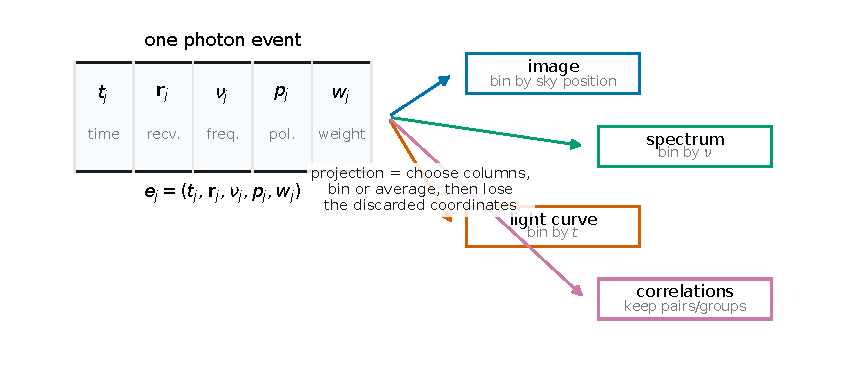
\includegraphics[width=0.9\linewidth]{figures/generated/chapter_01/ch01_event_table_map.pdf}
\caption{同一张光子事件表可以被投影成许多种数据产品。沿位置分箱得到图像，沿频率分箱得到光谱，沿时间分箱得到光变曲线，沿偏振通道组合得到偏振量。每一次投影都保留一部分信息、丢掉一部分信息；而“光子如何两两一起到达”这类关系，只有回到原始事件表才看得见。}
\label{fig:e00-event-map}
\end{figure}

\section{光有两种语言：波，与计数}
\label{sec:e00-two-languages}

要读懂事件表里“被丢掉的东西”，你得先接受一件让物理学家争论了一个世纪的事：\textbf{光同时说着两种语言}，而这两种语言描述的是同一件事。

第一种是\textbf{波的语言}。在一段足够窄的颜色里，光可以被看成一列振荡的电磁波：真正在抖动的是电场，它有振幅、有相位、会干涉。把两束光叠在一起，波峰对波峰就更亮，波峰对波谷就变暗——这就是相长与相消。相位、干涉、条纹，是这门语言的关键词。可见光的电场每秒要振荡上百万亿次，一个周期只有几飞秒（\(\mathrm{fs}=10^{-15}\,\mathrm{s}\)），快到任何普通探测器都跟不上；于是探测器看不见电场的正负摆动，只能把这些飞快的振荡在自己的响应时间里抹平，最后留下能量。

第二种是\textbf{计数的语言}。探测器留下的是一个个离散的“咔哒”，每一次都是一个光子的点击。既然是一次次独立的随机点击，计数就必然带有涨落：哪怕天体亮度、望远镜、探测器都纹丝不动，你数出来的每毫秒光子数也会上下抖动。这种与生俱来的抖动叫\textbf{散粒噪声}（shot noise，也叫泊松噪声），它不是仪器不好，而是“光本来就是一颗颗数出来的”这件事的必然影子。

这两种语言听起来南辕北辙——一个讲连续的波和相位，一个讲离散的点击和概率——但量子天文学的全部魅力，就在于它们其实是同一枚硬币的两面，而且能在\textbf{事件表}里被同时读出来。这里我先只做一个预告，把三条线索埋下：

\begin{itemize}
  \item 波的语言（电场、复振幅、相位、干涉）会在第~\ref{chap:e01} 章被正式接上，我们会把电场写成一支“旋转的箭头”；紧接着第~\ref{chap:e02} 章用傅里叶分析把它延伸开来，讲清带宽与相干时间——也就是“这支箭头能记住自己相位多久”。
  \item 计数的语言（概率、泊松统计、散粒噪声）会在第~\ref{chap:e03} 章被讲透，我们会从最朴素的“把时间切成许多小格”一路推到泊松分布，把“咔哒”的涨落算成一个可预言的数。
  \item 有了这两门语言，我们还要先把“光子”本身讲严谨：第~\ref{chap:e04} 章补上量子力学与谐振子的阶梯算符，第~\ref{chap:e05} 章据此给出光的量子化。这才是把“波”和“计数”真正缝在同一套数学里的针线。
  \item 而把这两种语言彻底焊在一起、让“波的相干”直接变成“计数的关联”的那座桥——强度干涉与 Hanbury Brown--Twiss（HBT）效应——属于全书第 2 部“相干与关联”，要到那里、也就是比光的量子化更靠后的章节，才正式搭起来。
\end{itemize}

换句话说，本章埋下的悬念——“同一批光子怎样一起到达，藏着什么”——它的答案要靠这两种语言合起来才能说清。第~\ref{chap:e01} 到第~\ref{chap:e05} 章先把两门语言各自打磨锋利、并把“光子”定义严谨；真正让二者合流的 HBT 关联，则留到后面的“相干与关联”部分去收网。

\section{本书的承诺：为什么值得学这门“量子”语言}
\label{sec:e00-promise}

你也许会问：传统天文学已经能给出图像、光谱、光变和偏振，日子过得好好的，为什么还要费劲去学这套“回到事件表、盯着光子怎样一起到达”的量子语言？因为它能做到一些传统方法\textbf{原理上做不到}的事。这不是把“量子”当噱头，而是有真金白银的科学回报。

\textbf{测量恒星的真实大小。} 恒星离我们太远，在望远镜里几乎都只是一个点。它们的角直径（angular diameter）小到毫角秒（milliarcsecond, mas，即 \(10^{-3}\) 角秒）乃至微角秒的量级。这有多小？\(1\,\mathrm{mas}\approx4.85\times10^{-9}\,\mathrm{rad}\)，要让一枚直径约 \(2.5\,\mathrm{cm}\) 的硬币张成这么小的角，你得把它放到约五千公里外——差不多是北京到伦敦一半的距离；而微角秒还要再小一千倍。普通望远镜受衍射极限所限根本看不出这么小的角结构，但强度干涉能把两台相隔百米、公里的望远镜的光子计数关联起来，从“两台望远镜的涨落有多同步”里反推出这个角直径。恒星不再是一个点，而有了可测量的圆盘、有了被自转压扁的形状、有了边缘的昏暗。

\textbf{逼近黑洞与致密天体的边缘。} 更长的基线、更高的时间分辨，原则上能把这套方法推向更小的角尺度，去约束吸积盘、恒星风、乃至致密天体周围的结构。

\textbf{给新物理套上绳索。} 光子到达时间与关联的极端精确测量，还能被用来检验一些超出标准模型的设想。凡是能写成“事件表里的一个可估计量 + 一份诚实的误差预算 + 一个 null test”的问题，都可能成为一个真正可执行的观测项目。

这些不是纸上谈兵。请记住三个真实的名字，它们会在全书反复出现：

\begin{itemize}
  \item \textbf{Narrabri}——上世纪六十年代，澳大利亚 Narrabri 的恒星强度干涉仪用两台可以在轨道上滑动的大反射器，第一次系统地量出了几十颗亮星的角直径。这是这门手艺的起点。
  \item \textbf{VERITAS} 与 \textbf{MAGIC}——如今，本为捕捉高能伽马射线而建的大型切伦科夫望远镜阵列（每台口径十几米），被巧妙地改造成光学强度干涉仪，测出了亮星亚毫角秒级的角直径，精度好到几个百分点。当年因信号太弱而沉寂多年的方法，靠着大镜面、高速电子学和数字关联器，重新活了过来。
\end{itemize}

图~\ref{fig:e00-science-map} 把这些科学目标摆在同一张地图上：横看是“离常规观测有多近”，纵看是“能带来多少传统方法拿不到的新信息”。亮星角直径已经近在咫尺，而更远处，是超新星测距、量子网络望远镜这样价值极高、也更需要工程突破的目标。这张图，就是本书想邀请你一起去探索的疆域。

\begin{figure}[tbp]
\centering
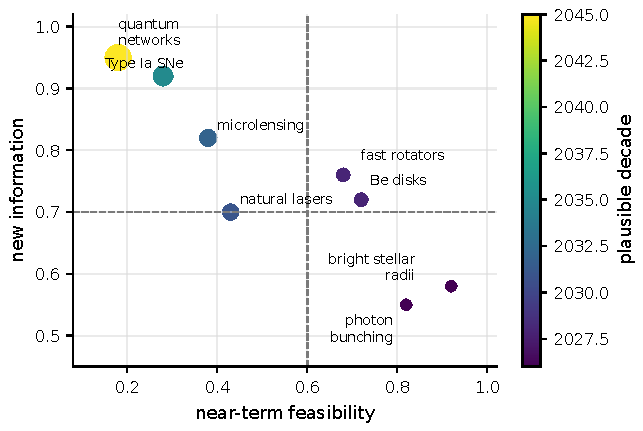
\includegraphics[width=0.8\linewidth]{figures/generated/chapter_02/ch02_science_case_map.pdf}
\caption{量子天文学第一代科学问题的地图：横轴大致表示离常规观测的远近，纵轴表示相对传统方法新增的信息量。亮星角直径和恒星光子聚束已经贴近现有能力；快速自转星、恒星盘、自然激射是近期扩展；超新星角距离测距、量子网络望远镜价值最高，但需要更长基线、快速触发或量子链路等工程突破。}
\label{fig:e00-science-map}
\end{figure}

\section{全书地图：我们要一起走的七站}
\label{sec:e00-map}

最后，摊开整张地图。本书分成七个部分（第 0 到第 6 部），像一条从地基一路盖到屋顶的施工路线。你不必一口气读完，但最好知道每一站在盖哪一层：

\begin{itemize}
  \item \textbf{第 0 部——地基与语言。} 就是你正在读的这几章。我们打磨两件工具：波的语言（电场、复振幅、相位、干涉）和计数的语言（泊松统计、散粒噪声、数量级估算）。目标是让你在遇到任何一条公式时，都先看得见它背后的物理画面。
  \item \textbf{第 1 部——光的量子描述。} 把“光子”这个词讲严谨：从电场的量子化，到相干态（coherent state）、热态（thermal state）与数态，理解为什么激光般的相干光和恒星般的热光，在“光子怎样一起到达”上如此不同。
  \item \textbf{第 2 部——相干与关联。} 本书的心脏。一阶相干 \(g^{(1)}\)（干涉、可见度）与二阶相干 \(g^{(2)}\)（光子聚束、强度关联）在这里登场，Siegert 关系把二者焊接起来，HBT 效应从“怪异现象”变成“可算的物理”。
  \item \textbf{第 3 部——从关联到成像。} van Cittert--Zernike 定理告诉我们，天空的亮度分布如何编码进空间相干度；于是“两台望远镜的关联”被翻译成“恒星的角直径”，强度干涉成像的原理在此闭环。
  \item \textbf{第 4 部——测量的极限。} 引入 Fisher 信息与 Cramér--Rao 下界，回答一个诚实的问题：给定这么多光子、这么长积分时间，我们\textbf{最好}能把角直径测到多准？噪声预算在这里被摆上台面。
  \item \textbf{第 5 部——真实的仪器与观测。} 大气、探测器抖动、死时间、背景、时钟同步、多台望远镜的 \(u,v\) 覆盖——把理想公式落到 Narrabri、VERITAS、MAGIC 这样真实系统的泥地里。
  \item \textbf{第 6 部——前沿与展望。} 频率与偏振关联、自然激射、微透镜、量子增强测量与量子网络望远镜，把地图的边界推向仍在探索的远方。
\end{itemize}

\textbf{这本书该怎么用？} 如果你是本科生，请按顺序读，把每一条带 \verb|formulaexplain| 小注的公式都当作一张“提示卡”，先读正文的物理画面，再回头核对每个符号的单位与意义，遇到推导不要跳步——书里已经把中间每一步都写出来了，你要做的是跟着走一遍。如果你已经有基础，可以直接跳到第 2 部的 \(g^{(2)}\) 与第 4 部的信息极限，那里是全书信息密度最高的地方。无论从哪进来，记得随时回头看一眼这张地图，问自己一句：\emph{我现在站在哪一站，手里这件工具是为了盖哪一层？}

\section{本章要点}
\label{sec:e00-summary}

\begin{itemize}
  \item 望远镜存下的不是波、也不是图像，而是一张带标签的\textbf{光子事件表}，每一行是 \(e_j=(t_j,\bm r_j,\nu_j,p_j,w_j)\)：时间、位置、频率通道、偏振/电子学通道、质量权重。
  \item 图像、光谱、光变曲线、偏振量，都是对这张表沿不同列做的\textbf{投影}；每次投影都保留一部分、丢掉一部分信息，而“光子如何两两一起到达”只在原始事件表里看得见。
  \item 光同时说\textbf{波的语言}（电场、相位、干涉）和\textbf{计数的语言}（点击、泊松噪声）；第~\ref{chap:e01} 到第~\ref{chap:e03} 章把这两门语言各自打磨清楚（波与相干时间在第~\ref{chap:e01}、\ref{chap:e02} 章，泊松与散粒噪声在第~\ref{chap:e03} 章），第~\ref{chap:e04}、\ref{chap:e05} 章再把“光子”定义严谨；真正让二者合流的 HBT 关联，留到第 2 部“相干与关联”去收网。
  \item 学这门语言的回报是实打实的：毫角秒乃至微角秒的\textbf{恒星角直径}、致密天体边缘、对新物理的约束；Narrabri、VERITAS、MAGIC 已经把它从概念做成了测量。
\end{itemize}

\medskip
\noindent\textbf{想一想。}
\begin{itemize}
  \item 如果你只被允许保留事件表里的\textbf{一列}，你会保留哪一列？为了回答“恒星有多大”，哪一列最不能丢？
  \item 同样一段观测，压成一幅图像和压成一条光变曲线，各自丢掉了什么、留下了什么？有没有哪种信息，两种投影都留不住？
  \item “散粒噪声”不是仪器缺陷，而是光被一颗颗数出来的必然。那么，把积分时间加长一倍，相对涨落大约会变成原来的多少？（提示：想想 \(1/\sqrt{\mu}\)。）
\end{itemize}

\chapter{波、相位与复振幅：干涉的最小语言}
\label{chap:e01}

\begin{chapteropening}
想象你站在一座望远镜的焦点后面，一束星光刚刚落进来。它在物理上是什么？是一段飞快摆动的电场——快到什么程度呢？一个来回只要几飞秒，比你眨一次眼快上万亿倍。可是当这束光最终变成数据时，那飞快的摆动却"消失"了，探测器只留下一个安静的数字：强度，或者说光子计数。摆动去哪了？相位又去哪了？

本章要做的事，就是把"波的语言"从最底层讲起：先写下一段单色电磁波，再学会用一支"旋转的箭头"（复振幅）同时装下它的振幅和相位；然后弄清楚探测器为什么只看得见振幅的平方、看不见相位本身；最后让两束光相遇，看干涉是怎么把"看不见的相位差"重新变成"看得见的亮暗"。这几件事，是后面所有相干、干涉、强度关联章节共同的字母表。
\end{chapteropening}

\section{单色电磁波：一段飞快摆动的电场}
\label{sec:e01-wave}

先把画面立起来。在一个足够窄的频率通道里，星光可以近似当成一列\textbf{单色光}（monochromatic light）：它只有一个频率，像一根纯音。真正在振荡的，是空间某一点上的电场强度——它随时间上上下下，像一根被拨动后稳定摆动的弦。数学上把它写成

\begin{equation}
  E(t)=E_0\cos(\omega t+\phi),\qquad \omega=2\pi\nu .
  \label{eq:e01-monochromatic}
\end{equation}
\begin{formulaexplain}
\(E(t)\) 是 \(t\) 时刻的电场；\(E_0\) 是振幅（摆动的最大幅度）；\(\omega\) 是角频率，\(\nu\) 是普通频率，二者相差一个 \(2\pi\)；\(\phi\) 是初相位，决定 \(t=0\) 时摆到了哪儿。
\end{formulaexplain}

逐个符号落地。\(E(t)\) 是电场，在 CGS 单位里量纲是 \({\rm statvolt\,cm^{-1}}\)，但对本章的推导来说，它具体多大并不重要，重要的是它\emph{怎样随时间变化}。\(E_0\) 是这段摆动的最大高度，也就是振幅（amplitude），它同样是电场的量纲。\(\phi\) 是初相位（phase），单位是弧度，是一个纯粹的角度、无量纲——你可以把它读成"在 \(t=0\) 这一刻，摆动进行到了周期里的哪个位置"。

括号里的 \(\omega t+\phi\) 整体叫\textbf{瞬时相位}（instantaneous phase）：随着时间流逝，\(\omega t\) 均匀增大，余弦就一遍遍地从 \(+1\) 荡到 \(-1\) 再荡回来。角频率 \(\omega\) 的单位是 \({\rm rad\,s^{-1}}\)，它告诉我们相位涨得多快；普通频率 \(\nu\)（单位 Hz，即每秒多少个整周期）与它的关系是 \(\omega=2\pi\nu\)，因为绕一整圈是 \(2\pi\) 弧度。周期是 \(T=1/\nu=2\pi/\omega\)。

现在代入真实数字，感受一下这有多快。可见光的频率大约在

\[
  \nu\simeq 4\times10^{14}\ {\rm Hz}\ (\text{红光})\quad\text{到}\quad 8\times10^{14}\ {\rm Hz}\ (\text{蓝光}),
\]

于是一个周期只有

\[
  T=\frac{1}{\nu}\simeq\frac{1}{5\times10^{14}\ {\rm Hz}}=2\times10^{-15}\ {\rm s}=2\ {\rm fs}.
\]

也就是说，可见光的电场每两飞秒就完成一次完整的上下摆动。飞秒（\(10^{-15}\) 秒）是什么概念？光在一飞秒里只跑 \(0.3\ \mu{\rm m}\)，还不到一根头发丝直径的百分之一。任何常规天文探测器——无论是 CCD 像素、光电倍增管还是雪崩二极管——它的响应时间至少是纳秒（\(10^{-9}\) 秒）量级，比一个光学周期慢了 \(10^{5}\)–\(10^{6}\) 倍（拿"至少 \(1\ {\rm ns}\)"去比"约 \(2\ {\rm fs}\)"，\(1\ {\rm ns}/2\ {\rm fs}\approx5\times10^{5}\)；若换成积分时间到微秒量级的 CCD，那就更慢）。

这就带来一个贯穿全书的关键事实：探测器"太慢"了，它根本跟不上电场逐周期的正负摆动。在探测器眨一次“电子学的眼”的时间里，电场已经上下荡了几十万乃至上百万个来回。它不可能把每一次摆动都记下来，只能把这些飞快的振荡在自己的响应时间里\emph{抹平}，最后留下一个平均能量。于是 \(E(t)\) 里那个飞快变化的、带着相位信息的部分，探测器\textbf{直接看不见}。我们后面会看到，正是这一点逼着人们去发明干涉与关联测量——那是把"看不见的相位"重新变回"看得见的强度"的唯一办法。

\section{复振幅：把振幅和相位装进一支旋转箭头}
\label{sec:e01-phasor}

式~\eqref{eq:e01-monochromatic} 有点笨重：每次讨论两束光相加、相位差怎么变，都要摆弄一堆余弦的和差化积公式。有没有更聪明的记法，能把\emph{振幅}和\emph{相位}这两件事一次装好、还让加法变简单？有，这就是\textbf{复振幅}（complex amplitude，也叫 phasor，相量）。

先给画面。把余弦想成一支从原点出发、绕着原点匀速旋转的箭头在水平轴上的投影：箭头的\emph{长度}就是振幅 \(E_0\)，箭头指向的\emph{角度}就是瞬时相位 \(\omega t+\phi\)。箭头以角速度 \(\omega\) 逆时针转\footnote{这里选了 \(e^{+i\omega t}\) 这一支时间约定：箭头逆时针旋转，正频率取 \(+i\omega t\)。本章之内它完全自洽，所有结论都不受影响。提醒一句以免日后对接时困惑：等到后面引入正/负频率场算符 \(\hat E^{(+)},\hat E^{(-)}\) 做二次量子化时，含湮灭算符 \(\hat a\) 的正频率部分 \(\hat E^{(+)}\) 通常按 \(e^{-i\omega t}\) 演化，箭头转向与这里相反。两种约定只是同一物理的镜像记法——把这里所有的 \(i\) 换成 \(-i\)（等价于把箭头看成顺时针转）即可平滑对接，物理内容一字不改。}，它在实轴（水平方向）上的影子，正好就是 \(E_0\cos(\omega t+\phi)\)。于是"一段振荡的场"被翻译成"一支旋转的箭头"。既然要描述平面上的箭头，用复数最自然——复平面上一个点，天生就带着"长度"和"角度"两个信息。

我们把箭头在 \(t=0\) 时刻的样子（长度 \(E_0\)、角度 \(\phi\)）打包成一个复数：

\begin{equation}
  \mathcal{E}=E_0e^{i\phi},\qquad E(t)=\operatorname{Re}\!\left[\mathcal{E}\,e^{i\omega t}\right].
  \label{eq:e01-phasor}
\end{equation}
\begin{formulaexplain}
\(\mathcal E\) 是复振幅；它的模 \(|\mathcal E|=E_0\) 是振幅，辐角 \(\arg\mathcal E=\phi\) 是相位。乘上旋转因子 \(e^{i\omega t}\) 让箭头转起来，再取实部 \(\operatorname{Re}\)（取水平影子），就还原出真实电场 \(E(t)\)。
\end{formulaexplain}

来验证这个记法确实还原了式~\eqref{eq:e01-monochromatic}。用欧拉公式 \(e^{i\theta}=\cos\theta+i\sin\theta\)（这是复指数的定义，本书会反复用到它），逐步展开：

\[
  \mathcal{E}\,e^{i\omega t}
  =E_0e^{i\phi}\,e^{i\omega t}
  =E_0\,e^{i(\omega t+\phi)}
  =E_0\bigl[\cos(\omega t+\phi)+i\sin(\omega t+\phi)\bigr].
\]

取实部（丢掉带 \(i\) 的虚部）：

\[
  \operatorname{Re}\!\left[\mathcal{E}\,e^{i\omega t}\right]
  =E_0\cos(\omega t+\phi)=E(t).
\]

一步不差，正是原来的电场。所以复振幅 \(\mathcal E\) 里没有丢任何信息：\(|\mathcal E|=|E_0e^{i\phi}|=E_0\) 给出振幅，\(\arg\mathcal E=\phi\) 给出相位。\(\mathcal E\) 与电场同量纲，而 \(e^{i\phi}\) 那部分是无量纲的纯方向。

这套记法的好处，要到下一节两束光相加时才真正显现：余弦相加很麻烦，但复数相加就是箭头首尾相接的向量加法，简单得多。这也是为什么从现在起，我们几乎总是先在复振幅的世界里算账，最后再取实部或取模落回真实世界。

\section{强度：探测器为什么只看得见振幅的平方}
\label{sec:e01-intensity}

回到那个核心问题：探测器看不见飞快摆动，那它到底记录了什么？答案是\textbf{强度}（intensity），也就是电场平方在响应时间内的平均。物理上，探测器吸收的是光的能量，而电磁场携带的能量密度正比于场的平方。所以探测器留下的量正比于 \(\langle E^2(t)\rangle\)，这里尖括号表示"在探测器响应时间内做时间平均"。

我们把这个平均一步步算出来，不跳步。从 \(E(t)=E_0\cos(\omega t+\phi)\) 出发：

\[
  E^2(t)=E_0^2\cos^2(\omega t+\phi).
\]

关键的一步，是用余弦的倍角恒等式 \(\cos^2\theta=\tfrac12\bigl[1+\cos(2\theta)\bigr]\)（这是标准三角恒等式，可由 \(\cos 2\theta=2\cos^2\theta-1\) 反解得到）把平方拆开：

\[
  E^2(t)=E_0^2\cdot\frac{1+\cos\!\bigl(2\omega t+2\phi\bigr)}{2}
  =\frac{E_0^2}{2}+\frac{E_0^2}{2}\cos\!\bigl(2\omega t+2\phi\bigr).
\]

现在做时间平均。右边第一项 \(E_0^2/2\) 是常数，平均还是它自己。第二项是一个以 \(2\omega\)（两倍光频，周期更短）飞快振荡的余弦——在探测器那么长的响应时间里，它上上下下荡了无数个完整周期，正的部分和负的部分刚好抵消，平均值为零。这正是上一节说的"抹平"：

\[
  \bigl\langle\cos(2\omega t+2\phi)\bigr\rangle_{\rm det}\approx 0
  \quad\Longrightarrow\quad
  \bigl\langle E^2(t)\bigr\rangle_{\rm det}=\frac{E_0^2}{2}.
\]

于是探测器留下的强度正比于

\begin{equation}
  I\ \propto\ \bigl\langle E^2(t)\bigr\rangle_{\rm det}=\frac{E_0^2}{2}=\frac{1}{2}\,|\mathcal E|^2 .
  \label{eq:e01-intensity}
\end{equation}
\begin{formulaexplain}
\(I\) 是探测到的强度；\(\langle\cdots\rangle_{\rm det}\) 是在探测器响应时间内的时间平均；那个 \(1/2\) 正是 \(\cos^2\) 一个周期平均的结果；\(|\mathcal E|^2\) 是复振幅的模平方。相位 \(\phi\) 在最终结果里\emph{消失}了。
\end{formulaexplain}

请特别盯住这条式子最后消失的东西：\(\phi\) 不见了。强度只依赖振幅 \(E_0\)（或者说 \(|\mathcal E|\)），完全不依赖相位。这从复振幅的角度看更是一目了然——\(|\mathcal E|^2=|E_0e^{i\phi}|^2=E_0^2\)，那个 \(e^{i\phi}\) 的模是 1，取模平方时相位因子被彻底吃掉。那支旋转箭头无论初始指向哪个方向，只要长度一样，测得的强度就一样。

物理上这句话是全书的一块基石：\textbf{单束光的相位不会被探测器直接记录}。它像一个藏起来的自由度，你手里的强度数据对它一无所知。那前面章节又说相位很重要，这不矛盾吗？不矛盾——单独一束光的绝对相位确实测不到，但两束光的\emph{相位差}可以，因为相位差会改变合成箭头的长度，从而改变强度。这正是干涉的用武之地，我们马上就去看。

（一个记号约定：那个恒定的 \(1/2\) 以及各种几何、效率因子在后文常被吸收进比例常数里，写成 \(I\propto|\mathcal E|^2\)。本章把 \(1/2\) 明写出来，是为了让"抹平快速振荡"这一步看得清清楚楚。）

\section{两束光相遇：干涉是怎么把相位差变回亮暗的}
\label{sec:e01-interference}

现在让两束单色光——比如来自同一颗星、经过两条不同路径——落到同一个探测器上。关键的物理次序是：\textbf{先相加的是电场，后平方的是强度}。这个次序不能反。因为电磁场满足叠加原理，两束光在同一点的电场是矢量相加；而探测器测的是相加\emph{之后}那个合成场的能量。用复振幅来做这件事最省力——两支箭头首尾相接，向量加法而已。

设两束光的复振幅分别是 \(\mathcal E_1\) 和 \(\mathcal E_2\)，合成场的复振幅就是 \(\mathcal E_1+\mathcal E_2\)。强度正比于它的模平方：

\begin{equation}
  I\ \propto\ |\mathcal E_1+\mathcal E_2|^2
  =|\mathcal E_1|^2+|\mathcal E_2|^2+2\,\operatorname{Re}\!\bigl(\mathcal E_1\mathcal E_2^{\ast}\bigr).
  \label{eq:e01-interference}
\end{equation}
\begin{formulaexplain}
\(\mathcal E_1,\mathcal E_2\) 是两束光的复振幅；前两项 \(|\mathcal E_1|^2,|\mathcal E_2|^2\) 是各自单独的强度；第三项 \(2\operatorname{Re}(\mathcal E_1\mathcal E_2^{\ast})\) 是\emph{干涉项}，星号 \({}^\ast\) 表示复共轭。是这一项让总强度多了或少了。
\end{formulaexplain}

先把这个展开老老实实推一遍。对任意复数 \(z\)，模平方就是它乘自己的共轭：\(|z|^2=z\,z^{\ast}\)。令 \(z=\mathcal E_1+\mathcal E_2\)，它的共轭是 \(\mathcal E_1^{\ast}+\mathcal E_2^{\ast}\)，逐项相乘：

\[
  |\mathcal E_1+\mathcal E_2|^2
  =(\mathcal E_1+\mathcal E_2)(\mathcal E_1^{\ast}+\mathcal E_2^{\ast})
  =\mathcal E_1\mathcal E_1^{\ast}+\mathcal E_2\mathcal E_2^{\ast}
  +\mathcal E_1\mathcal E_2^{\ast}+\mathcal E_2\mathcal E_1^{\ast}.
\]

前两项就是 \(|\mathcal E_1|^2\) 和 \(|\mathcal E_2|^2\)。后两项 \(\mathcal E_1\mathcal E_2^{\ast}\) 与 \(\mathcal E_2\mathcal E_1^{\ast}\) 互为共轭，而"一个复数加它的共轭等于它实部的两倍"（\(z+z^{\ast}=2\operatorname{Re}z\)），所以它们合起来正是 \(2\operatorname{Re}(\mathcal E_1\mathcal E_2^{\ast})\)。这就得到了式~\eqref{eq:e01-interference}。

接下来把复振幅的显式形式代进去，让相位现身。写 \(\mathcal E_1=E_1e^{i\phi_1}\)、\(\mathcal E_2=E_2e^{i\phi_2}\)，先算那个乘积：

\[
  \mathcal E_1\mathcal E_2^{\ast}
  =E_1e^{i\phi_1}\cdot E_2e^{-i\phi_2}
  =E_1E_2\,e^{i(\phi_1-\phi_2)}
  =E_1E_2\bigl[\cos(\phi_1-\phi_2)+i\sin(\phi_1-\phi_2)\bigr].
\]

取实部，虚部丢掉，干涉项就变成

\[
  2\,\operatorname{Re}\!\bigl(\mathcal E_1\mathcal E_2^{\ast}\bigr)
  =2E_1E_2\cos(\phi_1-\phi_2).
\]

于是两束光的总强度写成

\[
  I\ \propto\ E_1^2+E_2^2+2E_1E_2\cos(\phi_1-\phi_2).
\]

看这条式子的最后一项：它只依赖\textbf{相位差} \(\Delta\phi=\phi_1-\phi_2\)，不依赖两个绝对相位各自是多少。这正好呼应上一节的结论——绝对相位测不到，但相位差能通过强度显形。分三种情形读它：

\begin{itemize}
  \item \textbf{相长干涉}（constructive）：\(\Delta\phi=0\)（或 \(2\pi\) 的整数倍），\(\cos\Delta\phi=+1\)，干涉项取最大正值。两支箭头同向叠加，合成箭头最长，强度冲到峰值 \(E_1^2+E_2^2+2E_1E_2=(E_1+E_2)^2\)。若 \(E_1=E_2=E_0\)，峰值是 \(4E_0^2\)——是单束强度 \(E_0^2\) 的\emph{四}倍，而不是两倍。多出来的能量正是干涉"重新分配"的结果。
  \item \textbf{相消干涉}（destructive）：\(\Delta\phi=\pi\)，\(\cos\Delta\phi=-1\)，干涉项取最大负值。两支箭头反向，合成箭头最短，强度跌到谷底 \((E_1-E_2)^2\)。等强时 \(E_1=E_2\)，这里\emph{全黑}。
  \item \textbf{被平均掉}：如果相位差 \(\Delta\phi\) 不稳定，在测量时间里飞快地、无规律地乱变（两束光"记不住"彼此的相位），那么 \(\cos\Delta\phi\) 时正时负，平均下来趋于零，干涉项消失，只剩 \(I\propto E_1^2+E_2^2\)，两束光像不相干的路灯一样简单相加。这种"相位差还稳不稳"的问题，就是\textbf{相干性}（coherence），它是从第~\ref{chap:e05} 章起整本书的主角。
\end{itemize}

一句话收束这一节：干涉是一台"相位差翻译机"——它把探测器本来看不见的相位差 \(\Delta\phi\)，翻译成看得见的亮暗（强度的高低）。整本书讲的各种干涉与关联测量，骨子里都是在用不同的花样读取这个 \(\cos\Delta\phi\)。

\begin{figure}[tbp]
\centering
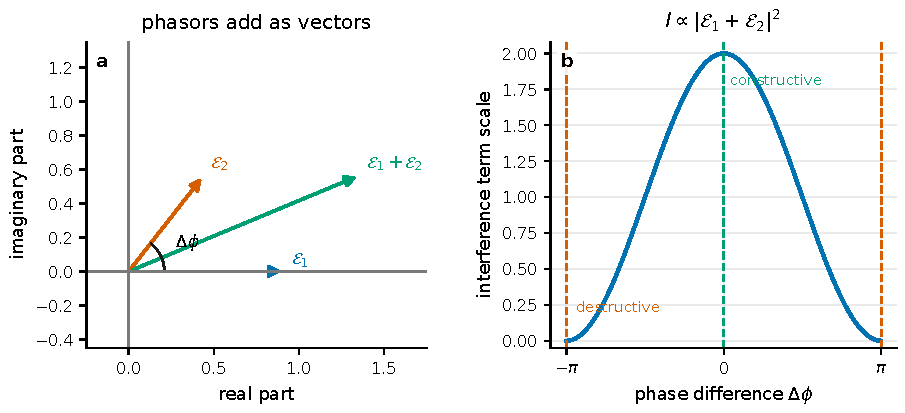
\includegraphics[width=0.85\linewidth]{figures/generated/chapter_01/ch01_phase_interference.pdf}
\caption{复振幅与两束光干涉的基本图像。复振幅是一支箭头，长度是振幅、方向是相位；两束光先做箭头的向量相加，探测器再取合成箭头长度的平方。相位差 \(\Delta\phi\) 决定干涉项是加强（相长）、抵消（相消），还是在相位乱变时被平均掉。}
\label{fig:e01-phase-interference}
\end{figure}

\section{几何相位：路程差是从哪儿来的}
\label{sec:e01-geometry}

上一节的相位差 \(\Delta\phi\) 还很抽象。在天文观测里，它最常见的来源其实非常具体、非常几何：\textbf{两束光走的路不一样长}。这一节就把这个"路程差"一步步变成相位差。

先立画面。设有一颗很远的星，它发出的光到达地面时，波前（同相位的面）几乎是一张平的大纸，沿着源方向 \(\bm s\)（一个指向星的单位矢量）推进。地面上有两台望远镜，位置相差一个\textbf{基线矢量}（baseline）\(\bm B\)——就是从第一台指向第二台的那根矢量，单位是厘米。因为两台望远镜不在垂直于 \(\bm s\) 的同一张波前上，同一个波前要先到达其中一台、再多走一小段才到另一台。这"多走的一小段"，就是路程差。

多走的路有多长？把基线 \(\bm B\) 投影到源方向 \(\bm s\) 上即可。矢量在某方向上的投影长度正是点积，所以路程差是

\[
  \Delta \ell=\bm B\cdot\bm s .
\]

这一步的几何含义要看清：\(\bm B\cdot\bm s=|\bm B|\cos\theta\)，\(\theta\) 是基线与源方向的夹角。若星就在基线正前方（\(\bm B\) 与 \(\bm s\) 平行），投影最长、路程差最大；若星在基线的正上方（\(\bm B\perp\bm s\)），投影为零、两台望远镜到同一波前的路一样长、没有路程差。这跟日常经验一致：斜着照过来的光，两个接收点之间才有先后。

现在把“多走的一段路”换算成“多转的相位”。这里要用到一个到目前为止还没正式点破、但马上就能从第~\ref{sec:e01-wave} 节的图像自己推出来的事实：波在空间里每前进一个\textbf{波长}（wavelength）\(\lambda\)，相位恰好前进 \(2\pi\)（转满一圈）。为什么？回到第~\ref{sec:e01-wave} 节立好的时间图像——电场每过一个周期 \(T\)，瞬时相位就增加 \(\omega T=2\pi\)（这正是“一个周期转满一圈”的定义）。而在同样这段时间 \(T\) 里，以光速 \(c\) 传播的波正好前进一段距离

\[
  \lambda\ \equiv\ cT=\frac{c}{\nu}=\frac{2\pi c}{\omega}.
\]

这段"相位刚好累积满一圈 \(2\pi\)"所对应的空间长度，就是波长。于是"时间上过了一个周期"和"空间上前进了一个波长"是同一件事的两种说法，相位都恰好前进 \(2\pi\)。这样一来，\(\lambda\) 并不是凭空冒出来的新符号：它由第~\ref{sec:e01-wave} 节反复打磨的 \(\nu\)（或 \(\omega\)）通过 \(\lambda=c/\nu\) 直接定出。代入那里的可见光频率 \(\nu\simeq5\times10^{14}\ {\rm Hz}\)，得 \(\lambda=c/\nu\approx(3\times10^{10}\ {\rm cm\,s^{-1}})/(5\times10^{14}\ {\rm Hz})=6\times10^{-5}\ {\rm cm}=0.6\ \mu{\rm m}\)，正是我们熟悉的可见光波长——和第~\ref{sec:e01-wave} 节"光在一飞秒里跑 \(0.3\ \mu{\rm m}\)"的数字也自洽（两飞秒一个周期，正好跑 \(0.6\ \mu{\rm m}\) 一个波长）。

有了这个"一个波长折算 \(2\pi\)"的汇率，路程差就好换算了：既然多走一个 \(\lambda\) 相位就多转 \(2\pi\)，那么多走 \(\Delta\ell\) 这么长，就是多走了 \(\Delta\ell/\lambda\) 个波长，相位前进了 \(\Delta\ell/\lambda\) 圈，也就是 \(2\pi\times(\Delta\ell/\lambda)\) 弧度。把 \(\Delta\ell=\bm B\cdot\bm s\) 代进去：

\begin{equation}
  \Delta\phi=\frac{2\pi}{\lambda}\,\bm B\cdot\bm s .
  \label{eq:e01-geometric-phase}
\end{equation}
\begin{formulaexplain}
\(\Delta\phi\) 是两束光的几何相位差；\(\bm B\) 是两接收点之间的基线矢量；\(\bm s\) 是源方向单位矢量；\(\bm B\cdot\bm s\) 是投影出来的路程差；前面的 \(2\pi/\lambda\) 是"每个波长折算 \(2\pi\) 相位"的换算系数。
\end{formulaexplain}

把每个部件再点一遍，确保单位对得上。\(\bm B\cdot\bm s\) 是长度，单位厘米；\(\lambda\) 也是长度，单位厘米；两者相除得到"走了多少个波长"，是个无量纲的数；再乘 \(2\pi\)（弧度/圈），就得到无量纲但以弧度计的相位差 \(\Delta\phi\)。量纲严丝合缝。那个 \(2\pi/\lambda\) 常被记作波数 \(k=2\pi/\lambda\)，于是也写成 \(\Delta\phi=k\,\bm B\cdot\bm s\)——它的意思始终是“把长度翻译成相位的汇率”。

代入真实数字，感受一下这个相位差有多大。恒星强度干涉的经典装置——Narrabri 恒星强度干涉仪——最大基线约 \(B\simeq188\ {\rm m}\)、工作波长约 \(\lambda\simeq0.44\ \mu{\rm m}\)；今天用 VERITAS、MAGIC 这类切伦科夫望远镜阵列做强度干涉时，基线也在上百米量级。取一组整齐的代表值 \(B\sim100\ {\rm m}=10^{4}\ {\rm cm}\)、\(\lambda\sim0.5\ \mu{\rm m}=5\times10^{-5}\ {\rm cm}\)，当基线几乎正对源方向时，路程差最大可达 \(\Delta\ell\sim B=100\ {\rm m}\)，于是

\[
  \frac{\Delta\ell}{\lambda}\sim\frac{10^{4}\ {\rm cm}}{5\times10^{-5}\ {\rm cm}}=2\times10^{8}\ (\text{个波长}),\qquad
  \Delta\phi=2\pi\,\frac{\Delta\ell}{\lambda}\sim1.3\times10^{9}\ {\rm rad}.
\]

相位差高达十亿弧度、合两亿多整圈！这就点出了干涉测量的一个基本事实：绝对相位差本身是个天文数字，没人真的去数它一共转了多少整圈。真正被测量、被关心的，是当地球自转让基线 \(\bm B\) 相对源方向 \(\bm s\) 缓慢转动、或者源在天上的位置稍有不同时，这个庞大的 \(\Delta\phi\) 又变化了几圈——也就是干涉条纹\emph{移动了多少个周期}。绝对相位是天文数字，条纹的\emph{相对}移动才是可测、可用的信号。

这条式子看着简单，却是干涉测量的整个出发点：把它代回上一节的 \(2E_1E_2\cos(\Delta\phi)\)，望远镜看到的干涉亮暗就直接和基线 \(\bm B\)、源方向 \(\bm s\) 挂上了钩——转动地球（改变 \(\bm B\) 相对 \(\bm s\) 的投影），或者源的位置稍有不同，条纹就会移动。反过来，从条纹怎么移动，就能反推源在天上的精细结构。不过这里我们只搭好最基础的相位语言；两台望远镜之间更完整的空间相干关系，要到第~\ref{chap:e05} 章及其之后才被正式发展起来。

\section{本章要点}
\label{sec:e01-summary}

\begin{itemize}
  \item 单色光的物理本体是飞快摆动的电场 \(E(t)=E_0\cos(\omega t+\phi)\)；可见光周期只有几飞秒，比任何常规探测器快约百万倍，所以逐周期的振荡与相位探测器\textbf{看不见}。
  \item 复振幅 \(\mathcal E=E_0e^{i\phi}\) 是一支旋转箭头：长度 \(|\mathcal E|=E_0\) 是振幅，方向 \(\arg\mathcal E=\phi\) 是相位。取实部 \(E(t)=\operatorname{Re}[\mathcal E e^{i\omega t}]\) 就还原真实电场；箭头记法让"场的相加"变成简单的向量相加。
  \item 强度 \(I\propto\langle E^2\rangle_{\rm det}=\tfrac12|\mathcal E|^2\)。那个 \(1/2\) 来自 \(\cos^2\) 在一个周期上的平均；快速振荡项被抹平，\emph{单束光的绝对相位不被记录}。
  \item 两束光先加电场后平方：\(I\propto|\mathcal E_1+\mathcal E_2|^2=|\mathcal E_1|^2+|\mathcal E_2|^2+2E_1E_2\cos(\phi_1-\phi_2)\)。干涉项只认相位差：\(\Delta\phi=0\) 相长、\(\Delta\phi=\pi\) 相消、相位乱变则被平均掉。干涉是把看不见的相位差翻译成看得见的亮暗。
  \item 天文里最常见的相位差来自几何路程差 \(\Delta\phi=(2\pi/\lambda)\,\bm B\cdot\bm s\)：\(\bm B\cdot\bm s\) 是基线在源方向上的投影程差，\(2\pi/\lambda\) 把长度换成相位。它是空间相干与干涉成像的起点（第~\ref{chap:e05} 章）。
\end{itemize}

\vspace{0.5em}
\noindent\textbf{想一想。}
(1) 两束等强度的光相长干涉时，峰值强度是单束的四倍——那"多出来的能量"从哪里来，又到哪里去了？
(2) 如果把两台望远镜的基线 \(\bm B\) 转到正好垂直于源方向 \(\bm s\)，几何相位差 \(\Delta\phi\) 等于多少？此时干涉条纹会怎样？
(3) 为什么说"绝对相位测不到，但相位差测得到"这两句话并不矛盾？试着只用式~\eqref{eq:e01-intensity} 和式~\eqref{eq:e01-interference} 来回答。

\chapter{傅里叶、带宽与相干时间}
\label{chap:e02}

\begin{chapteropening}
上一章我们把光看成"一支飞快旋转的复振幅箭头"，也承认探测器太慢、只能记录被抹平后的强度。可是"太慢"到底相对于什么？光的相位又能维持多久不乱？要回答这些问题，得先学会一门通用的语言：任何一段波，无论多么复杂，都可以拆成一堆纯粹的单频正弦——就像一段和弦总能分解成一个个纯音。本章先把这门"拆音"的语言（傅里叶分析，Fourier analysis）讲清楚，再用它推出三个后面要反复用到的量：带宽 \(\Delta\nu\)、相干时间 \(\tau_c\)，以及把两者联系起来的自相关与功率谱。读完你会明白，为什么一个纳秒级的时间门里，其实塞进了成百上千个"相干时间"。
\end{chapteropening}

\section{任何波都是纯音的叠加}
\label{sec:e02-fourier-idea}

先建立画面。想象你手里有一段随时间变化的信号 \(f(t)\)：它可以是一根琴弦的位移，也可以是探测面上某一点的电场。傅里叶的洞见是：这段信号从来都不是"一整块"，而是许多不同频率的纯正弦波叠在一起的结果。低频的正弦画出大轮廓，高频的正弦补上尖锐的细节；把它们按各自的"份量"加起来，就还原出原信号。这份"每个频率占多少份量"的清单，就叫这个信号的\textbf{频谱}（spectrum）。

先看最容易想象的情形：信号是周期性的，周期为 \(T\)，也就是 \(f(t+T)=f(t)\)。这时候允许出现的频率不是连续的，而是一梯一梯的谐波：基频 \(\nu_1=1/T\)，以及它的整数倍 \(\nu_n=n/T\)。傅里叶级数（Fourier series）说，这样的周期信号可以写成
\begin{equation}
  f(t)=\sum_{n=-\infty}^{+\infty} c_n\,e^{\,i\,2\pi\nu_n t},
  \qquad
  \nu_n=\frac{n}{T},
  \label{eq:e02-fourier-series}
\end{equation}
\begin{formulaexplain}
\(f(t)\) 是周期为 \(T\) 的信号；\(\nu_n=n/T\) 是第 \(n\) 条谐波频率；复系数 \(c_n\) 是这条谐波在信号里所占的"份量"（含振幅与相位）。整条式子说：周期信号是一叠离散纯音之和。
\end{formulaexplain}
这里每一项 \(e^{i2\pi\nu_n t}\) 就是一支"以频率 \(\nu_n\) 匀速旋转的单位箭头"，复系数 \(c_n\) 决定这支箭头有多长（振幅）、初始指向哪里（相位）。由于 \(e^{i2\pi\nu_n t}\) 是无量纲的纯相位因子，信号 \(f(t)\) 的量纲便全部由复系数 \(c_n\) 承载；\(\nu_n\) 的单位是赫兹（\({\rm Hz}={\rm s^{-1}}\)）。要取出某一条谐波的份量，只需把信号和那条谐波"对一对拍子"——在一个周期内做积分，正交性会让其余谐波全部相消，只留下我们想要的一项：
\[
  c_n=\frac{1}{T}\int_{0}^{T} f(t)\,e^{-\,i\,2\pi\nu_n t}\,dt .
\]
其中用到的关键事实是不同谐波相互正交：\(\frac{1}{T}\int_0^T e^{i2\pi(m-n)t/T}\,dt=\delta_{mn}\)（当 \(m=n\) 时被积函数恒为 1，积分给 1；当 \(m\neq n\) 时是一个整周期的复指数，正负相消给 0）。这是我们第一次点名使用的"已知结果"，后面反复要用。

现在把周期 \(T\) 想象成越来越长。谐波的间隔 \(\Delta\nu=\nu_{n+1}-\nu_n=1/T\) 越来越密；当 \(T\to\infty\)，信号不再周期，一梯一梯的离散频率就融成一条连续的频率轴。这里最容易被跳过的一步是：级数里那个归一化因子 \(1/T\) 到底去哪了？把它交代清楚只需一个小技巧——在合成式 \eqref{eq:e02-fourier-series} 里给每一项配一个"频率间隔"因子 \(\Delta\nu\)（记住 \(\Delta\nu=1/T\)），乘一个再除一个，等式不变：
\[
  f(t)=\sum_{n} c_n\,e^{\,i2\pi\nu_n t}
      =\sum_{n} \frac{c_n}{\Delta\nu}\,e^{\,i2\pi\nu_n t}\,\Delta\nu .
\]
这一步什么也没改，只是把整条求和整理成了标准的黎曼和形状 \(\sum_n g(\nu_n)\,\Delta\nu\)——每一项都带着它所占的那一小格频率宽度 \(\Delta\nu\)。当 \(T\to\infty\) 时 \(\Delta\nu\to d\nu\)，黎曼和就收敛成积分，离散频率 \(\nu_n\) 变成连续变量 \(\nu\)，而括号里的组合 \(c_n/\Delta\nu\) 收敛到一条连续的\textbf{频谱密度}
\[
  \tilde f(\nu)\;=\;\frac{c_n}{\Delta\nu}\;=\;c_n\,T .
\]
于是 \(1/T\) 的下落就闭合了：它并没有凭空消失，而是被 \(\Delta\nu=1/T\) 吸收进了积分测度 \(d\nu\) 里，代价是频谱密度 \(\tilde f(\nu)\) 比原来的级数系数 \(c_n\) 大了整整 \(T\) 倍（这也和分析式对得上——把 \(c_n=\frac1T\int_0^T f\,e^{-i2\pi\nu_n t}dt\) 两边乘 \(T\)，右边的 \(1/T\) 正好消掉，留下的就是 \(\tilde f(\nu)=\int f\,e^{-i2\pi\nu t}dt\)）。这样求和 \(\sum_n\) 就干净地变成了积分 \(\int d\nu\)，我们也就从傅里叶级数过渡到了傅里叶变换（Fourier transform）。剩下的收敛数学细节我们不去纠缠，只保留这个物理直觉：非周期信号的频谱是连续的，每一个频率都可能出场，各自带着自己的份量。傅里叶变换对写成
\begin{equation}
  \tilde f(\nu)=\int_{-\infty}^{+\infty} f(t)\,e^{-\,i\,2\pi\nu t}\,dt,
  \qquad
  f(t)=\int_{-\infty}^{+\infty} \tilde f(\nu)\,e^{+\,i\,2\pi\nu t}\,d\nu .
  \label{eq:e02-fourier-transform}
\end{equation}
\begin{formulaexplain}
左式把时间信号 \(f(t)\) "拆"成频谱 \(\tilde f(\nu)\)；右式把频谱"合"回信号。\(e^{\mp i2\pi\nu t}\) 是频率为 \(\nu\) 的纯音。一拆一合互为逆运算，信息量不增不减。
\end{formulaexplain}
两式互为逆变换：左边（分析式）像用一排调好的音叉去"听"信号里每个频率有多强，右边（合成式）像把这些纯音按份量重新奏响、拼回原信号。要注意 \(\tilde f(\nu)\) 一般是复数：它的模 \(|\tilde f(\nu)|\) 说这个频率占多少份量，它的辐角说这个频率成分的相位。若把频率轴换成波长轴，这正是光谱仪吐出的那条谱线曲线的抽象版本。整本书后面谈"谱线宽度""滤光片带宽""相干函数"，底层用的都是这一对式子。

一句话小结：傅里叶变换是一台"拆音—合音"机器，把"随时间变化"翻译成"由哪些频率组成"。接下来我们让它干第一件真正有用的活。

\section{有限长的波包：时间越短，频率越宽}
\label{sec:e02-wavepacket}

真实的光从不是一列无限长、单一频率的完美正弦。恒星原子每发一次光，只辐射极短一小段波列就被碰撞打断；滤光片也只放行一小段频率。于是我们面对的总是\textbf{波包}（wave packet）：一段有头有尾、频率也不完全单一的振荡。这里藏着一条贯穿全书的铁律：\emph{一段波在时间上越短，它在频率上就越宽}；反过来，要频率极纯，就得让波列极长。

为什么？直觉是这样的：一列无限长的完美正弦，只需要一个频率就能描述，频谱是一根针。可一旦你把它"剪短"——乘上一个有限宽度的包络——就等于强行在两端把它掐灭，而"掐灭"这个动作本身需要额外的频率成分来完成（就像要奏出一个极短促的"哒"，必须动用很宽的一段音域）。波列越短，掐得越急，需要的频率越宽。用数量级写出来就是著名的
\begin{equation}
  \Delta\nu\,\Delta t \;\gtrsim\; 1 ,
  \label{eq:e02-bandwidth-time}
\end{equation}
\begin{formulaexplain}
\(\Delta t\) 是波包在时间上的持续宽度，\(\Delta\nu\) 是它在频率上的展宽。二者之积不能小于约 1：时间越窄，频率必然越宽。这是傅里叶变换的普适约束，不是仪器缺陷。
\end{formulaexplain}
式中 \(\Delta t\) 的单位是秒、\(\Delta\nu\) 的单位是赫兹，乘积无量纲。请注意这不是海森堡不确定性原理，而是纯经典波动性质；量子力学的 \(\Delta E\,\Delta t\gtrsim\hbar\) 只是把它乘上 \(E=h\nu\) 后的翻版。式 \eqref{eq:e02-bandwidth-time} 里的"\(\gtrsim\)"提醒我们它是量级关系，具体系数取决于怎样定义"宽度"和包络形状。下面就用一个能算到底的例子，把这条不等式变成等号。

\paragraph{高斯波包的显式计算}

取一个高斯包络调制的振荡，写成复数形式最省事：
\[
  f(t)=e^{-\,t^{2}/(2\sigma_t^{2})}\;e^{\,i\,2\pi\nu_0 t}.
\]
这里 \(\nu_0\) 是载波频率（可见光约 \(6\times10^{14}\,{\rm Hz}\)），\(\sigma_t\) 是包络的时间宽度（单位：秒）：\(|f|\) 在 \(t=0\) 达到峰值，在 \(|t|\sim\sigma_t\) 处衰减到峰值的 \(e^{-1/2}\)。我们来求它的频谱 \(\tilde f(\nu)\)。代入定义式 \eqref{eq:e02-fourier-transform}：
\[
  \tilde f(\nu)=\int_{-\infty}^{+\infty}
  e^{-\,t^{2}/(2\sigma_t^{2})}\,e^{\,i\,2\pi\nu_0 t}\,e^{-\,i\,2\pi\nu t}\,dt
  =\int_{-\infty}^{+\infty}
  e^{-\,t^{2}/(2\sigma_t^{2})}\,e^{-\,i\,2\pi(\nu-\nu_0)t}\,dt .
\]
把指数并成"二次型 + 一次项"的标准形式，令 \(a=\dfrac{1}{2\sigma_t^{2}}\)、\(b=i\,2\pi(\nu-\nu_0)\)，被积函数是 \(e^{-a t^{2}-b t}\)。这里要点名使用一个已知结果——\textbf{高斯积分}的配方公式：
\[
  \int_{-\infty}^{+\infty} e^{-a t^{2}-b t}\,dt
  =\sqrt{\frac{\pi}{a}}\;e^{\,b^{2}/(4a)},
  \qquad(a>0).
\]
（它的来路是把指数配方成 \(-a(t+\tfrac{b}{2a})^2+\tfrac{b^2}{4a}\)，再用最基本的 \(\int e^{-a u^2}du=\sqrt{\pi/a}\)。）代入 \(a,b\)：
\[
  \sqrt{\frac{\pi}{a}}=\sqrt{2\pi}\,\sigma_t,
  \qquad
  \frac{b^{2}}{4a}
  =\frac{\bigl[i\,2\pi(\nu-\nu_0)\bigr]^{2}}{4/(2\sigma_t^{2})}
  =\frac{-4\pi^{2}(\nu-\nu_0)^{2}}{2/\sigma_t^{2}}
  =-2\pi^{2}\sigma_t^{2}(\nu-\nu_0)^{2}.
\]
于是频谱是
\begin{equation}
  \tilde f(\nu)=\sqrt{2\pi}\,\sigma_t\;
  e^{-\,2\pi^{2}\sigma_t^{2}(\nu-\nu_0)^{2}}.
  \label{eq:e02-gaussian-spectrum}
\end{equation}
\begin{formulaexplain}
高斯波包的频谱仍是一条高斯，中心在载波频率 \(\nu_0\)。指数里 \(\sigma_t\) 越大（波列越长），频率高斯越窄。时间与频率两条高斯宽度成反比。
\end{formulaexplain}
这是一个漂亮的自洽结果：\emph{高斯的傅里叶变换还是高斯}。把式 \eqref{eq:e02-gaussian-spectrum} 的指数写成标准高斯 \(e^{-(\nu-\nu_0)^2/(2\sigma_\nu^2)}\) 的样子，读出频率宽度：
\[
  \frac{1}{2\sigma_\nu^{2}}=2\pi^{2}\sigma_t^{2}
  \quad\Longrightarrow\quad
  \sigma_\nu=\frac{1}{2\pi\,\sigma_t}.
\]
时间宽度 \(\sigma_t\) 与频率宽度 \(\sigma_\nu\) 果然成反比。把它们相乘，载波、振幅这些细节全部约掉，只剩一个纯数：
\begin{equation}
  \sigma_t\,\sigma_\nu=\frac{1}{2\pi}\approx0.16 .
  \label{eq:e02-gaussian-product}
\end{equation}
\begin{formulaexplain}
高斯波包让时间宽度与频率宽度之积取到最小值 \(1/2\pi\)。任何其它形状的波包只会更大。这就是式 \eqref{eq:e02-bandwidth-time} 里"\(\gtrsim 1\)"的精确下限版本。
\end{formulaexplain}
这里要当心一个数字上的"张力"：\(1/2\pi\approx0.16\) 和式 \eqref{eq:e02-bandwidth-time} 里的"\(\gtrsim1\)"看起来差了约 6 倍，读者难免要问"下限怎么会是 0.16 而不是 1"。答案全在"宽度"二字的口径上。式 \eqref{eq:e02-gaussian-product} 里的 \(\sigma_t,\sigma_\nu\) 是振幅高斯的\emph{标准差}，而实验上常说的"宽度"往往指\emph{半高全宽}（FWHM）\(\Delta\)。对高斯而言二者的换算是 \(\Delta=2\sqrt{2\ln2}\,\sigma\approx2.35\,\sigma\)，于是
\[
  \Delta\nu\,\Delta t=(2.35)^2\,\sigma_\nu\sigma_t
  \approx\frac{2.35^2}{2\pi}\approx0.88\sim1 .
\]
可见一旦改用半高全宽度量，乘积立刻回到量级 1，和式 \eqref{eq:e02-bandwidth-time} 完全吻合。所以 \(1/2\pi\) 与 1 并不矛盾，它们只差一个"你把宽度定义成标准差还是半高全宽"所决定的数值系数——物理是同一条，数字随口径浮动。明白了这一点，就可以放心地把量级不等式 \eqref{eq:e02-bandwidth-time} 落到实处：高斯波包是"时间—频率同时最紧凑"的极端情形，取到下限；换成方波包络、洛伦兹线型或被碰撞随机打断的波列，乘积只会更大，但量级都是 1。所以无论光是怎么产生的，只要它持续了 \(\Delta t\)，它的频率就至少铺开约 \(1/\Delta t\) 那么宽。记住这一条，下一节我们就能把"带宽"和"相干时间"一口气算出来。图~\ref{fig:e02-wave-packet} 把这条铁律画成一目了然的对照。

\begin{figure}[tbp]
\centering
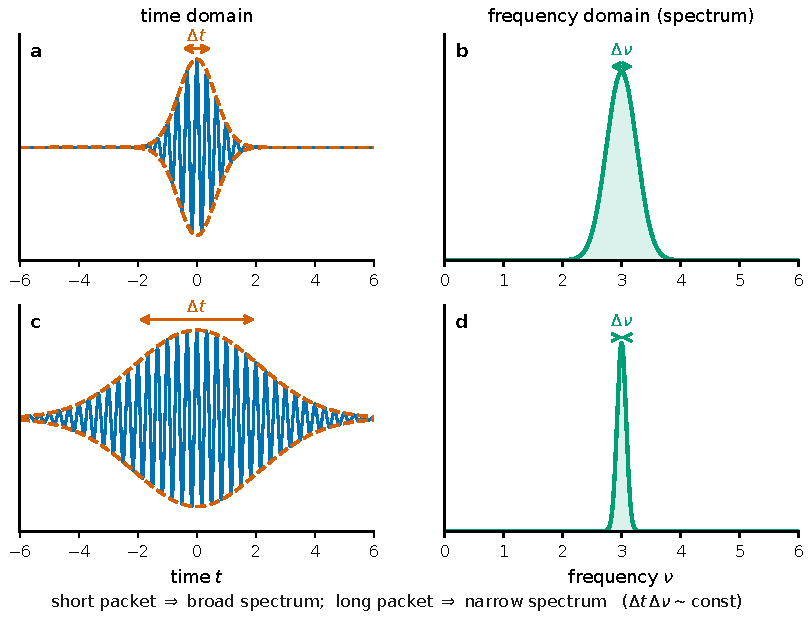
\includegraphics[width=0.9\linewidth]{figures/generated/edu_ch02/e02_wave_packet_spectrum.pdf}
\caption{有限长波包的"时间—频率互易"。上排是短波包：时间上被掐得很窄（\(\Delta t\) 小，橙色双箭头），频谱却铺得很宽（\(\Delta\nu\) 大）；下排是长波包：时间上拉得很长，频谱反而挤成一条窄峰。橙色虚线是包络，绿色是对应的频谱。两排的乘积 \(\Delta t\,\Delta\nu\) 都约为同一个常数——这正是式 \eqref{eq:e02-bandwidth-time} 的图像。}
\label{fig:e02-wave-packet}
\end{figure}

\section{把带宽算成真实数字}
\label{sec:e02-bandwidth}

天文观测里，我们通常不是直接知道频率带宽 \(\Delta\nu\)，而是知道滤光片的中心波长 \(\lambda\) 和波长带宽 \(\Delta\lambda\)（比如"500 纳米中心、1 纳米半宽"）。要把它翻成频率带宽，只需对 \(\nu\) 与 \(\lambda\) 的关系做一步微分。频率和波长由光速联系：
\[
  \nu=\frac{c}{\lambda}.
\]
这里 \(c\approx3\times10^{10}\,{\rm cm\,s^{-1}}\) 是光速；沿用全书的 CGS 单位约定，波长 \(\lambda\) 以厘米计、频率 \(\nu\) 以赫兹计。对 \(\lambda\) 求导，这一步不能跳——用 \(\dfrac{d}{d\lambda}\bigl(c\lambda^{-1}\bigr)=-c\lambda^{-2}\)：
\[
  \frac{d\nu}{d\lambda}=-\frac{c}{\lambda^{2}}.
\]
负号表示波长增大时频率减小，这是意料之中的反比关系；我们关心的是带宽的大小，取绝对值，并把微分 \(d\lambda\) 换成有限的小带宽 \(\Delta\lambda\)（只要 \(\Delta\lambda\ll\lambda\)，用微分近似有限差就足够精确）：
\begin{equation}
  \Delta\nu\;\simeq\;\frac{c\,\Delta\lambda}{\lambda^{2}} .
  \label{eq:e02-bandwidth-conversion}
\end{equation}
\begin{formulaexplain}
\(\Delta\nu\) 是频率带宽，\(\Delta\lambda\) 是波长带宽，\(\lambda\) 是中心波长，\(c\) 是光速。同样的 \(\Delta\lambda\)，波长越短（\(\lambda^2\) 越小），换算出的频率带宽越大。
\end{formulaexplain}
注意分母是 \(\lambda^{2}\) 而不是 \(\lambda\)：这提醒我们，同样"1 纳米"的波长窗口，在蓝端对应的频率带宽比红端更大。现在代入真实数字。取一片可见光滤光片，\(\lambda=500\,{\rm nm}=5\times10^{-5}\,{\rm cm}\)，\(\Delta\lambda=1\,{\rm nm}=1\times10^{-7}\,{\rm cm}\)：
\[
  \Delta\nu\simeq
  \frac{(3\times10^{10}\,{\rm cm\,s^{-1}})\times(1\times10^{-7}\,{\rm cm})}
       {(5\times10^{-5}\,{\rm cm})^{2}}
  =\frac{3\times10^{3}}{2.5\times10^{-9}}\,{\rm Hz}
  =1.2\times10^{12}\,{\rm Hz}.
\]
也就是约 \(1.2\,{\rm THz}\)（太赫兹）。请把这个数量级记牢：一片看起来"很窄"的 1 纳米滤光片，在频率上其实放行了一个上万亿赫兹宽的窗口。和载波频率 \(\nu_0\sim6\times10^{14}\,{\rm Hz}\) 相比，这个窗口只占 \(0.2\%\)，光谱学意义上确实"窄"；但换算成时间尺度以后，它会带来一个惊人的短。这正是下一节的主角。

\section{相干时间：波还记得自己相位多久}
\label{sec:e02-coherence-time}

现在把上一节的带宽翻译成时间。回到铁律 \eqref{eq:e02-bandwidth-time}：一段频率铺开 \(\Delta\nu\) 的光，在时间上最多只能保持约 \(\Delta t\sim1/\Delta\nu\) 的"协调"。给这个时间起个名字，叫\textbf{相干时间}（coherence time）\(\tau_c\)：
\begin{equation}
  \tau_c\;\simeq\;\frac{1}{\Delta\nu}
  \;\simeq\;\frac{\lambda^{2}}{c\,\Delta\lambda} .
  \label{eq:e02-coherence-time}
\end{equation}
\begin{formulaexplain}
\(\tau_c\) 是相干时间，单位秒；带宽 \(\Delta\nu\) 越宽，相干时间越短。第二个等号只是把式 \eqref{eq:e02-bandwidth-conversion} 代进来，用波长量表达。它是光"记得自己相位"的时长，不是探测器的时间分辨率。
\end{formulaexplain}
怎么理解 \(\tau_c\)？把光想成那支旋转的复振幅箭头。如果光是理想单频的，箭头就以恒定角速度匀速转，你只要看一眼此刻的指向，就能准确预言一微秒后、一小时后它指向哪里——它"永远记得"自己的相位。可真实的光有带宽：里面混着一大堆频率略有差别的箭头，它们转速稍有快慢，一开始还整齐，转着转着就散开了，合成箭头的相位越来越不可预测。\(\tau_c\) 就是"从整齐到散乱"所需的时间——过了 \(\tau_c\)，光基本已经忘了自己 \(\tau_c\) 之前的相位。带宽越宽，混进来的转速差别越大，忘得越快。

代入上一节的数字，\(\Delta\nu\simeq1.2\times10^{12}\,{\rm Hz}\)：
\[
  \tau_c\simeq\frac{1}{1.2\times10^{12}\,{\rm Hz}}
  \approx8.3\times10^{-13}\,{\rm s}
  \approx0.8\,{\rm ps}.
\]
不到一皮秒（picosecond，\(1\,{\rm ps}=10^{-12}\,{\rm s}\)）。这就是那片"很窄"的 1 纳米滤光片给出的相干时间：光只能记住自己的相位约 0.8 皮秒，然后就翻篇了。

这个数字之所以要用整章去准备，是因为它和探测器的能力之间有一道触目惊心的鸿沟。最快的单光子探测器（雪崩光电二极管 APD、光电倍增管 PMT）的时间响应大约在 100 皮秒到 1 纳秒之间。拿相干时间去比：
\[
  \frac{\Delta t_{\rm det}}{\tau_c}\sim
  \frac{100\,{\rm ps}\;\text{到}\;1\,{\rm ns}}{0.8\,{\rm ps}}
  \approx1.2\times10^{2}\;\text{到}\;1.2\times10^{3}.
\]
也就是说，探测器一个时间门（time bin）的宽度，是相干时间的\emph{成百上千倍}。换句话说，你每记录一个时间门的强度，其实是把成百上千段互不相干、各自独立的波列平均在了一起。探测器根本来不及看清任何单独一段波列的相位起伏；它看到的永远是一大堆相干时间被抹平后的平均能量。这个结论——"一个时间门里平均了 \(N\sim10^{2}\)--\(10^{3}\) 个相干时间"——会在后面讲光子统计、聚束、强度干涉时反复登场，并直接决定我们能测到的信号被稀释多少倍。

\begin{figure}[tbp]
\centering
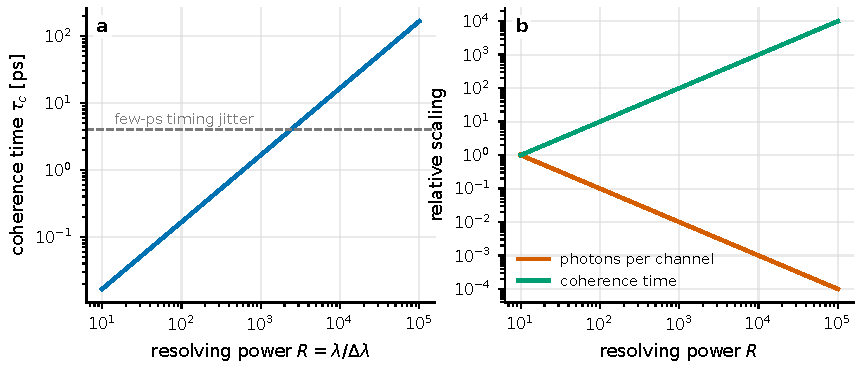
\includegraphics[width=0.85\linewidth]{figures/generated/chapter_06/ch06_spectral_resolution_coherence.pdf}
\caption{光谱分辨率与相干时间是同一件事的两面。谱线（带宽 \(\Delta\nu\)）越窄，对应的相干时间 \(\tau_c\simeq1/\Delta\nu\) 越长；反之宽带光的相干时间极短。图中把可见光宽带滤光片给出的 ps 量级 \(\tau_c\) 与探测器的 100\,ps--1\,ns 响应放在一起，可见一个时间门内包含了大量互不相干的波列。}
\label{fig:e02-spectral-coherence}
\end{figure}

小结一句：带宽和相干时间是同一枚硬币的两面，\(\tau_c\simeq1/\Delta\nu\)。可见光宽带下 \(\tau_c\) 短到皮秒，而探测器慢到百皮秒以上，二者相差百倍以上——这道鸿沟是后面一切强度测量的背景板。

\section{自相关与功率谱：走向相干函数}
\label{sec:e02-autocorrelation}

前面我们用"\(\tau_c\) 是相位记忆的时长"来描述相干时间，那是个定性说法。怎么把"记忆"量化成一条可计算、可测量的曲线？答案是\textbf{自相关函数}（autocorrelation function）。它的想法极其朴素：把信号和"延迟了 \(\tau\) 的自己"相乘再取平均，看它们还有多像。对一个（平稳的）信号 \(f(t)\)，定义
\begin{equation}
  \Gamma(\tau)=\bigl\langle f^{*}(t)\,f(t+\tau)\bigr\rangle
  =\lim_{T\to\infty}\frac{1}{T}\int_{0}^{T} f^{*}(t)\,f(t+\tau)\,dt ,
  \label{eq:e02-autocorrelation}
\end{equation}
\begin{formulaexplain}
\(\Gamma(\tau)\) 是自相关函数；\(\tau\) 是时间延迟；尖括号（或时间积分）表示对时间取平均；\(f^*\) 是复共轭。它衡量"信号此刻"与"信号在 \(\tau\) 之后"的相似程度。
\end{formulaexplain}
当延迟 \(\tau=0\) 时，\(\Gamma(0)=\langle|f|^{2}\rangle\) 就是信号的平均强度（正实数、最大值）。随着 \(\tau\) 增大，如果信号还"记得"自己，\(f^*(t)\) 与 \(f(t+\tau)\) 的相位仍步调一致，乘积平均后不会相消，\(\Gamma\) 保持较大；一旦 \(\tau\) 超过相干时间，两者相位早已各走各的、随机分布，正负乘积在平均中相互抵消，\(\Gamma\to0\)。所以\emph{自相关函数从峰值衰减到零的宽度，正是相干时间 \(\tau_c\)}。这就把上一节那个含糊的"记忆时长"变成了一条曲线的宽度——可算、可测。图~\ref{fig:e02-coherence} 左图正展示了这种衰减：带宽越宽，归一化的自相关掉得越快、相干时间越短；右图把 \(\tau_c\simeq1/\Delta\nu\) 这条标度画成了一条直线。

\begin{figure}[tbp]
\centering
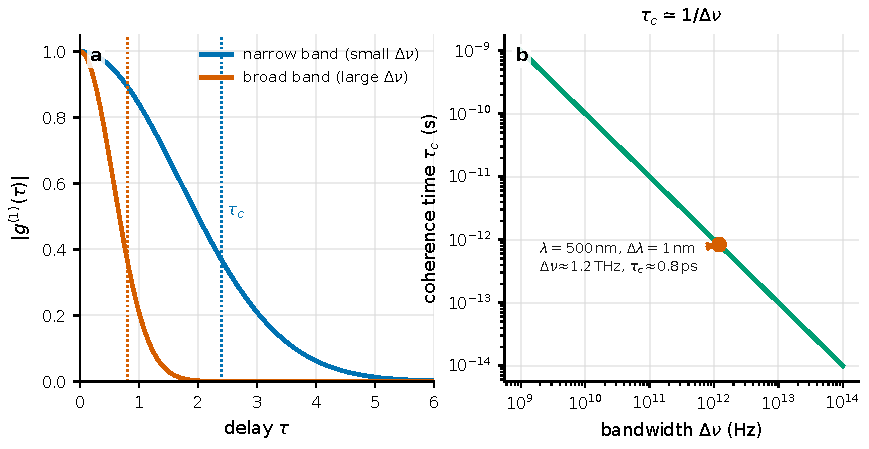
\includegraphics[width=0.92\linewidth]{figures/generated/edu_ch02/e02_coherence_bandwidth.pdf}
\caption{相干时间与带宽互为倒数。左：归一化自相关（也就是后面要正式定义的一阶相干度 \(|g^{(1)}(\tau)|\)）随延迟 \(\tau\) 衰减；带宽越宽（橙）掉得越快、相干时间 \(\tau_c\) 越短，带宽越窄（蓝）则"记得"越久。右：\(\tau_c\simeq1/\Delta\nu\) 在双对数坐标下是一条直线，橙点标出 \(500\,{\rm nm}\)、\(1\,{\rm nm}\) 滤光片给出的 \(\Delta\nu\approx1.2\,{\rm THz}\)、\(\tau_c\approx0.8\,{\rm ps}\)。}
\label{fig:e02-coherence}
\end{figure}

最后要点出一个漂亮而深刻的定理，它把本章两条主线（频谱与相干）系成一个结。这就是\textbf{维纳–辛钦定理}（Wiener–Khinchin theorem）：信号的\textbf{功率谱}（power spectrum）\(S(\nu)\)，恰好是它的自相关函数的傅里叶变换：
\begin{equation}
  S(\nu)=\int_{-\infty}^{+\infty}\Gamma(\tau)\,e^{-\,i\,2\pi\nu\tau}\,d\tau .
  \label{eq:e02-wiener-khinchin}
\end{equation}
\begin{formulaexplain}
\(S(\nu)\) 是功率谱，告诉你各频率占多少功率；\(\Gamma(\tau)\) 是自相关函数。二者是一对傅里叶变换。"信号里有哪些频率"与"信号记得自己多久"是同一件事的两种说法。
\end{formulaexplain}
这个定理的含义值得慢慢体会。它说：\emph{你不必真的去测频谱，只要测出自相关函数，做一次傅里叶变换就得到功率谱；反过来也一样}。这正是式 \eqref{eq:e02-bandwidth-time} 的严格化身——自相关的宽度（相干时间 \(\tau_c\)）与功率谱的宽度（带宽 \(\Delta\nu\)）是一对傅里叶伙伴，一个窄另一个必宽，乘积约为 1。回头看高斯波包那节：时间高斯和频率高斯互为傅里叶变换、宽度成反比，正是维纳–辛钦定理的一个具体样本。

为什么在一本天文书里要这么郑重其事地介绍自相关？因为式 \eqref{eq:e02-autocorrelation} 里那个 \(\langle f^*(t)f(t+\tau)\rangle\) 的结构，几乎原封不动就是后面要定义的\textbf{一阶相干函数}（first-order coherence function）\(g^{(1)}(\tau)\)——只要把 \(f\) 换成电场，再归一化。也就是说，本章的自相关函数就是相干函数的"经典彩排"。等我们在第 \ref{chap:e05} 章之后正式引入 \(g^{(1)}\) 和 \(g^{(2)}\) 时，你会发现它们并不神秘：\(g^{(1)}\) 量的就是电场的自相关（相位记忆），它的宽度就是这里的 \(\tau_c\)；而恒星的谱线形状与它之间，正由维纳–辛钦定理这座桥连接。本章搭好的这套语言——频谱、带宽、相干时间、自相关——就是整本相干理论的地基。

\section{本章要点}
\label{sec:e02-summary}

\begin{itemize}
  \item \textbf{傅里叶思想}：任何波都是纯音的叠加。周期信号给离散谐波（傅里叶级数），非周期信号给连续频谱（傅里叶变换，式 \eqref{eq:e02-fourier-transform}）。频谱就是"每个频率占多少份量"的清单。
  \item \textbf{时间—频率互易}：波列越短，频率越宽，\(\Delta\nu\,\Delta t\gtrsim1\)（式 \eqref{eq:e02-bandwidth-time}）。高斯波包取到最紧凑的下限 \(\sigma_t\sigma_\nu=1/2\pi\)，且其傅里叶变换仍是高斯。
  \item \textbf{带宽换算}：由 \(\nu=c/\lambda\) 微分得 \(\Delta\nu\simeq c\,\Delta\lambda/\lambda^{2}\)。500\,nm、1\,nm 滤光片给 \(\Delta\nu\approx1.2\times10^{12}\,{\rm Hz}\)。
  \item \textbf{相干时间}：\(\tau_c\simeq1/\Delta\nu\approx0.8\,{\rm ps}\)。它是光记得自己相位的时长。探测器 100\,ps--1\,ns 的响应比它长百到千倍——一个时间门平均了成百上千个相干时间。
  \item \textbf{自相关与功率谱}：自相关 \(\Gamma(\tau)\) 的衰减宽度就是 \(\tau_c\)；维纳–辛钦定理（式 \eqref{eq:e02-wiener-khinchin}）说功率谱是自相关的傅里叶变换。这正是一阶相干函数 \(g^{(1)}\) 的前身。
\end{itemize}

\noindent\textbf{想一想}：
\begin{enumerate}
  \item 如果把滤光片换成 \(10\,{\rm nm}\) 带宽，相干时间会变成多少？探测器一个 \(1\,{\rm ns}\) 时间门里又平均了多少个相干时间？
  \item 一列被碰撞平均每 \(\tau_c\) 打断一次的波列，它的谱线大约有多宽？（提示：用式 \eqref{eq:e02-bandwidth-time} 反推。）
  \item 为什么说"测自相关函数"和"测光谱"在信息上是等价的？维纳–辛钦定理在其中扮演什么角色？
\end{enumerate}

\chapter{概率、泊松过程与散粒噪声}
\label{chap:e03}

\begin{chapteropening}
在导览章（\ref{chap:e00}）里我们已经见到，望远镜最终交给我们的不是一条光滑的电磁波，而是一串离散的点击：某一时刻，某一像素，某一通道，"啪"地记录下一个光子。上一章（\ref{chap:e02}）我们又学会了用带宽和相干时间来刻画这束光作为"波"的一面；可这些波最终是被探测器一颗一颗数下来的。既然是"数"出来的，那就一定有涨落——同样一颗恒星，同样一台望远镜，你连着数十个毫秒，每个毫秒数到的光子数几乎不会相同。这不是仪器坏了，而是"计数"这件事本身自带的呼吸。

本章要把"计数的语言"一次讲透。我们先花几段话把概率论里最少量的几个词（随机变量、期望、方差、独立）复习清楚，然后从"把一段时间切成许多小格"这个极朴素的图像出发，一步不跳地推出泊松分布（Poisson distribution），再由此得到那条贯穿全书的黄金公式：均值等于方差，噪声正比于 $\sqrt{\mu}$。最后我们会问一个更深的问题——如果有一天你测到方差不等于均值，那意味着什么？这个"意味着什么"，正是后面专讲二阶相干 $g^{(2)}$ 的章节要展开的整个故事的入口。
\end{chapteropening}

\section{最小限度的概率复习}
\label{sec:e03-review}

在开始数光子之前，我们需要四个词。它们你在普通物理和概率课上都见过，这里只用"一段话加一个式子"的分量把它们钉牢，方便后面直接调用。

\paragraph{随机变量（random variable）。}
一个随机变量就是"一次实验会给出一个数，但你事先不知道是哪个数"。数一个毫秒里到达的光子数 $N$ 就是最典型的随机变量：它只能取非负整数 $0,1,2,\dots$，而且每个取值都对应一个概率。描述一个（离散）随机变量，就是给出它取每个值的概率 $P(N)$，满足
\begin{equation}
  P(N)\ge 0,\qquad \sum_{N=0}^{\infty}P(N)=1 .
  \label{eq:e03-normalization}
\end{equation}
\begin{formulaexplain}
$N$ 是一次测量得到的整数计数；$P(N)$ 是"这一次恰好数到 $N$ 个"的概率。第一式说概率非负，第二式说把所有可能情况的概率加起来必须是 $1$——总得发生点什么。
\end{formulaexplain}
这里 $N$ 是无量纲的整数（就是"几个"），$P(N)$ 也是无量纲的纯数，取值在 $0$ 到 $1$ 之间。式 \eqref{eq:e03-normalization} 的第二条叫归一化（normalization），它是后面所有推导都必须自洽满足的"守恒律"：不管我们把分布写成多复杂的样子，把 $N$ 从 $0$ 加到无穷，答案必须回到 $1$。

\paragraph{期望（expectation）。}
期望就是"平均值"，但它是一个理论上的、加权的平均：把每个可能取值 $N$ 乘上它的概率再求和。我们用尖括号 $\langle\cdot\rangle$ 表示求期望，
\begin{equation}
  \langle N\rangle=\sum_{N=0}^{\infty}N\,P(N).
  \label{eq:e03-expectation}
\end{equation}
\begin{formulaexplain}
$\langle N\rangle$ 读作"$N$ 的期望"或"$N$ 的平均"；它把每个可能的计数 $N$ 按其发生概率 $P(N)$ 加权求和。它不是某一次的结果，而是无穷多次重复后的平均归宿。
\end{formulaexplain}
注意 $\langle N\rangle$ 一般不是整数——平均每毫秒 $100.3$ 个光子完全合理，尽管任何一次你只能数到整数。期望是可加的：对任意两个随机变量 $X,Y$，$\langle X+Y\rangle=\langle X\rangle+\langle Y\rangle$，无论它们是否独立。这个"期望永远可加"的性质，稍后在拼装小格时会被反复使用。

\paragraph{方差（variance）。}
光有平均值还不够，我们还要知道"每次结果离平均值有多远"。方差衡量的就是涨落的大小：取偏差 $N-\langle N\rangle$，平方（这样正负偏差都变成正贡献），再求期望，
\begin{equation}
  \operatorname{Var}(N)=\big\langle (N-\langle N\rangle)^2\big\rangle
  =\langle N^2\rangle-\langle N\rangle^2 .
  \label{eq:e03-variance}
\end{equation}
\begin{formulaexplain}
$\operatorname{Var}(N)$ 是方差，度量计数围绕其平均值的散布程度；它等于"平方的平均"减去"平均的平方"。它越大，说明每一次数出来的结果越"飘"。
\end{formulaexplain}
式 \eqref{eq:e03-variance} 的第二个等号是一条恒等式，把定义展开即可：$\langle(N-\langle N\rangle)^2\rangle=\langle N^2-2N\langle N\rangle+\langle N\rangle^2\rangle=\langle N^2\rangle-2\langle N\rangle\langle N\rangle+\langle N\rangle^2=\langle N^2\rangle-\langle N\rangle^2$，这里用到了期望可加以及"常数的期望还是它自己"。方差的量纲是 $N$ 的量纲的平方（这里 $N$ 无量纲，所以方差也无量纲）。它的平方根
\[
  \sigma=\sqrt{\operatorname{Var}(N)}
\]
叫标准差（standard deviation），单位和 $N$ 相同，是我们日常说的"误差棒有多长"。请记住这个直觉：$\sigma$ 才是和 $N$ 可比的"涨落尺度"，方差是它的平方。

\paragraph{独立性（independence）。}
两个随机变量独立，直觉上就是"知道其中一个的结果，对另一个的概率分布毫无帮助"。用式子说，联合概率能分解成各自概率的乘积：$P(X=x,\,Y=y)=P(X=x)\,P(Y=y)$。独立性给我们一件极其好用的礼物——方差可加：
\begin{equation}
  \operatorname{Var}(X+Y)=\operatorname{Var}(X)+\operatorname{Var}(Y)
  \quad(\text{当 }X,Y\text{ 独立}).
  \label{eq:e03-var-additive}
\end{equation}
\begin{formulaexplain}
只有当 $X$ 与 $Y$ 相互独立时，它们之和的方差才等于各自方差之和。这条"独立则方差可加"是后面把许多小格拼成一个大 bin、从而算出散粒噪声的关键杠杆。
\end{formulaexplain}
对比一下：期望的可加性 $\langle X+Y\rangle=\langle X\rangle+\langle Y\rangle$ 是无条件的，而方差的可加性 \eqref{eq:e03-var-additive} 需要独立作为前提。原因藏在交叉项里：$\operatorname{Var}(X+Y)=\operatorname{Var}(X)+\operatorname{Var}(Y)+2\operatorname{Cov}(X,Y)$，其中协方差 $\operatorname{Cov}(X,Y)=\langle XY\rangle-\langle X\rangle\langle Y\rangle$ 度量两者的相关；独立时 $\langle XY\rangle=\langle X\rangle\langle Y\rangle$，协方差归零，方差才干净地相加。请把这句话记牢，因为本章末尾"方差不等于均值意味着什么"的整个悬念，就藏在这个协方差是不是零里。

有了这四个词，我们就可以开始真正地数光子了。

\section{一个时间 bin 里的平均计数}
\label{sec:e03-mean}

回到望远镜前。上一章里，探测器把光变成一串离散点击。现在我们做一件最朴素的事：选一个时间窗口（time bin），宽度记作 $\Delta t$，然后数一数这个窗口里落进了几个光子。

如果这束光的平均光子到达率（arrival rate）是 $R_\gamma$，那么一个 bin 里的平均计数就是率乘以时间：
\begin{equation}
  \mu=R_\gamma\,\Delta t .
  \label{eq:e03-mean-count}
\end{equation}
\begin{formulaexplain}
$\mu$ 是一个时间 bin 内的平均光子数（即 $\langle N\rangle$）；$R_\gamma$ 是平均到达率，单位 $\mathrm{s^{-1}}$；$\Delta t$ 是 bin 宽度，单位 $\mathrm{s}$。二者相乘，秒被消掉，$\mu$ 是无量纲的"平均几个"。
\end{formulaexplain}
让我们把单位和数量级坐实。$R_\gamma$ 的量纲是"每秒几个"，即 $\mathrm{s^{-1}}$；$\Delta t$ 的量纲是秒 $\mathrm{s}$；两者相乘，秒和"每秒"抵消，$\mu$ 就是一个纯数。取一组真实的光学观测数字：一颗中等亮度的恒星、一台米级望远镜、一个窄带通道，探测到的光子率大约 $R_\gamma=10^{5}\,\mathrm{s^{-1}}$；若我们把时间切成 $\Delta t=1\,\mathrm{ms}=10^{-3}\,\mathrm{s}$ 的 bin，则
\[
  \mu=R_\gamma\,\Delta t=10^{5}\,\mathrm{s^{-1}}\times10^{-3}\,\mathrm{s}=100 .
\]
也就是说，平均每个毫秒里落进来大约 $100$ 个光子。

这里"平均"两个字必须掰开揉碎地讲，因为它是本章一切的支点。式 \eqref{eq:e03-mean-count} 绝不是说"每个 $1\,\mathrm{ms}$ 窗口都精确收到 $100$ 个光子"。它说的是：如果你在完全相同的条件下（恒星一样亮、望远镜一样大、效率一样高）取来成千上万个 $1\,\mathrm{ms}$ 窗口，把每个窗口数到的光子数加起来除以窗口个数，这个"实测平均"会趋近 $100$。真实的事件流里，这一个 bin 也许是 $92$，下一个也许是 $107$，再下一个是 $100$——它们围着 $100$ 上下呼吸。$\mu$ 是这场呼吸的中心线，不是任何一次的实测值。

关键在于：即便你把一切外部条件都冻结住，让恒星、大气、望远镜、探测器都纹丝不动，这种呼吸也不会消失。这不是"测不准的仪器噪声"，而是"数离散东西"这个动作本身自带的统计涨落。要理解这份涨落到底服从什么规律、有多大，我们需要给"光子彼此独立地稀疏到达"这句物理直觉配上一套数学，那就是泊松分布。

\section{从二项分布到泊松分布：一步不跳的推导}
\label{sec:e03-poisson}

\paragraph{把 bin 切成许多小格}

我们要回答的问题是：既然平均值是 $\mu$，那么"恰好数到 $N$ 个"的概率 $P(N)$ 到底长什么样？

先立一个物理假设，它是整个泊松图像的灵魂：在给定平均率的前提下，光子彼此独立地、无记忆地到达。所谓"无记忆"是说，前一个光子刚到过，既不会招呼下一个也赶紧来（那是聚束），也不会警告下一个别来（那是反聚束）；每一段极短的时间里出不出现光子，只由这段时间的长短决定，和别处发生了什么无关。这正是上一节"平均"背后最简单的到达模式。本章先假设它成立，把结论算到底；至于它何时会被打破，留到最后一节点题。

有了这个假设，就可以用一个非常具体的图像来算。把宽度为 $\Delta t$ 的时间 bin 均匀切成 $M$ 个很短的小格，每个小格宽度
\[
  \delta t=\frac{\Delta t}{M}.
\]
只要 $M$ 足够大、$\delta t$ 足够短，每个小格里最多只可能有一个光子——两个光子同时挤进同一个极短小格的概率可以忽略。于是每个小格就退化成一次最简单的"抛硬币"：要么点击（出现一个光子），要么没有。一个小格发生点击的概率近似为
\begin{equation}
  p=R_\gamma\,\delta t .
  \label{eq:e03-cell-prob}
\end{equation}
\begin{formulaexplain}
$p$ 是单个小格里出现一次点击的概率；$R_\gamma$ 是到达率；$\delta t$ 是小格宽度。率越高、小格越长，这一格里逮到一个光子的机会越大——但只要 $\delta t$ 够短，$p$ 就是个很小的数。
\end{formulaexplain}
$p$ 是无量纲概率（$\mathrm{s^{-1}}\times\mathrm{s}$ 抵消成纯数）。注意这里有个自洽性检查：所有小格的平均点击数加起来，应当正好是整个 bin 的平均计数。确实，$M$ 个小格、每格平均贡献 $p$，总平均就是
\[
  M\,p=M\cdot R_\gamma\frac{\Delta t}{M}=R_\gamma\,\Delta t=\mu .
\]
这个 $Mp=\mu$ 是我们接下来取极限时唯一要"钉死不动"的量：无论把小格切得多细（$M\to\infty$，$p\to0$），乘积 $Mp$ 始终等于 $\mu$。

\paragraph{先写下二项分布}

现在数光子就变成了一道纯组合题："在 $M$ 个小格里，恰好有 $N$ 个格子发生了点击"的概率是多少？由于各小格相互独立，每一种"指定哪 $N$ 个格子点击、其余 $M-N$ 个格子没点击"的具体情形，概率都是 $p^{N}(1-p)^{M-N}$；而"从 $M$ 个格子里选出哪 $N$ 个点击"共有 $\binom{M}{N}$ 种方式。把方式数乘上每种情形的概率，得到二项分布（binomial distribution）：
\begin{equation}
  P_M(N)=\binom{M}{N}p^{N}(1-p)^{M-N},
  \qquad \binom{M}{N}=\frac{M!}{N!\,(M-N)!}.
  \label{eq:e03-binomial}
\end{equation}
\begin{formulaexplain}
$P_M(N)$ 是把 bin 切成 $M$ 个小格后、恰好 $N$ 格点击的概率。$p^{N}$ 是这 $N$ 格都点击、$(1-p)^{M-N}$ 是其余格都不点击、$\binom{M}{N}$ 是"选哪 $N$ 格"的方案数。三者相乘即得。
\end{formulaexplain}
这条式子还没有近似，它是把小格图像精确翻译成概率。$\binom{M}{N}$ 读作"$M$ 选 $N$"，是二项系数；$N!$（$N$ 的阶乘）是排列数的归一化因子，负责除掉"同样这几格、只是数它们的先后顺序不同"的重复。接下来要做的，就是让小格无限变细：$M\to\infty$、$p\to0$，同时死死摁住 $Mp=\mu$。我们把式 \eqref{eq:e03-binomial} 拆成三块——$\binom{M}{N}$、$p^N$、$(1-p)^{M-N}$——一块一块取极限。

\paragraph{\texorpdfstring{第一步：$\binom{M}{N}p^{N}\to \mu^{N}/N!$}{第一步：二项系数那一项的极限}}

把 $p=\mu/M$ 代进去（这是 $Mp=\mu$ 的改写），先合并二项系数和 $p^N$：
\[
  \binom{M}{N}p^{N}
  =\frac{M!}{N!\,(M-N)!}\left(\frac{\mu}{M}\right)^{N}
  =\frac{1}{N!}\cdot\frac{M!}{(M-N)!}\cdot\frac{\mu^{N}}{M^{N}} .
\]
中间那块 $\dfrac{M!}{(M-N)!}$ 其实就是 $N$ 个连续下降的因子相乘：
\[
  \frac{M!}{(M-N)!}=M(M-1)(M-2)\cdots(M-N+1) .
\]
它一共 $N$ 个因子，每个都近似等于 $M$（因为 $N$ 是固定的有限整数，而 $M$ 要趋于无穷，$M-1,M-2,\dots$ 相对于 $M$ 的差别可以忽略）。更精确地，把它除以 $M^{N}$：
\[
  \frac{M(M-1)\cdots(M-N+1)}{M^{N}}
  =1\cdot\Big(1-\tfrac{1}{M}\Big)\Big(1-\tfrac{2}{M}\Big)\cdots\Big(1-\tfrac{N-1}{M}\Big)
  \xrightarrow[M\to\infty]{}1 .
\]
每个括号在 $M\to\infty$ 时都趋于 $1$，而括号只有固定的 $N-1$ 个，所以整段乘积趋于 $1$。于是第一块的极限干净利落：
\begin{equation}
  \binom{M}{N}p^{N}
  =\frac{\mu^{N}}{N!}\cdot\frac{M(M-1)\cdots(M-N+1)}{M^{N}}
  \xrightarrow[M\to\infty]{}\frac{\mu^{N}}{N!}.
  \label{eq:e03-limit-first}
\end{equation}
\begin{formulaexplain}
把 $p=\mu/M$ 代入后，二项系数与 $p^N$ 合并；分子里 $N$ 个下降因子除以 $M^N$ 后逐个趋于 $1$，只剩下 $\mu^N/N!$。这一步把"选格子的组合数"化成了泊松公式里熟悉的 $\mu^N/N!$。
\end{formulaexplain}

\paragraph{\texorpdfstring{第二步：$(1-p)^{M}\to e^{-\mu}$}{第二步：不点击概率的极限}}

现在处理第三块 $(1-p)^{M-N}$。同样代入 $p=\mu/M$：
\[
  (1-p)^{M-N}=\Big(1-\frac{\mu}{M}\Big)^{M-N}
  =\Big(1-\frac{\mu}{M}\Big)^{M}\cdot\Big(1-\frac{\mu}{M}\Big)^{-N}.
\]
先看第二个因子 $\big(1-\mu/M\big)^{-N}$：指数 $-N$ 是固定的有限数，而底数 $1-\mu/M\to 1$，所以这个因子趋于 $1^{-N}=1$，可以扔掉。真正要紧的是第一个因子 $\big(1-\mu/M\big)^{M}$。这里我们点名调用一个标准极限——它就是自然常数 $e$ 的定义式的一般形式：
\begin{equation}
  \lim_{M\to\infty}\Big(1-\frac{\mu}{M}\Big)^{M}=e^{-\mu}.
  \label{eq:e03-elimit}
\end{equation}
\begin{formulaexplain}
这是一条已知的标准极限（$e$ 的定义式）：$\big(1+x/M\big)^{M}\to e^{x}$，取 $x=-\mu$ 即得 $e^{-\mu}$。它把"许多个小格都没点击"的联合概率，凝聚成一个指数因子。
\end{formulaexplain}
为什么 \eqref{eq:e03-elimit} 成立、而不是一句咒语？我们可以取对数验证一遍，用到对数的泰勒展开（Taylor expansion）$\ln(1+u)=u-\tfrac12u^{2}+\cdots$（当 $u$ 很小）：
\[
  \ln\Big(1-\frac{\mu}{M}\Big)^{M}
  =M\ln\Big(1-\frac{\mu}{M}\Big)
  =M\left(-\frac{\mu}{M}-\frac{\mu^{2}}{2M^{2}}-\cdots\right)
  =-\mu-\frac{\mu^{2}}{2M}-\cdots .
\]
当 $M\to\infty$ 时，除第一项外全部含 $1/M$ 的项都消失，只剩 $-\mu$；再取指数还原，就得到 $e^{-\mu}$。物理上，这个 $e^{-\mu}$ 正是"极多个小格、每个都恰好没有点击"的总概率的凝练：$M$ 个小格，每格不点击的概率是 $1-p$，全都不点击就是 $(1-p)^{M}$，在极限下就成了 $e^{-\mu}$。

\paragraph{合起来：泊松分布}

把两步的极限 \eqref{eq:e03-limit-first} 和 \eqref{eq:e03-elimit} 相乘（第二块里被扔掉的 $\big(1-\mu/M\big)^{-N}\to1$ 已并入），二项分布 \eqref{eq:e03-binomial} 就收敛到泊松分布：
\begin{equation}
  P(N)=\lim_{M\to\infty}P_M(N)
  =e^{-\mu}\,\frac{\mu^{N}}{N!}.
  \label{eq:e03-poisson}
\end{equation}
\begin{formulaexplain}
$P(N)$ 是在平均计数为 $\mu$ 时、一个 bin 里恰好数到 $N$ 个光子的概率。$e^{-\mu}$ 来自"许多小格都没点击"，$\mu^{N}$ 是平均越大越偏向多计数的权重，$N!$ 去掉点击排序的重复。这就是稀疏独立到达的计数律。
\end{formulaexplain}
这条式子里每个部件都有对应的直觉。指数因子 $e^{-\mu}$ 是"背景基调"，代表大量空小格的贡献，$\mu$ 越大它压得越低；$\mu^{N}$ 是"越亮越偏多"的爬升项；$N!$ 是组合归一化，抹平了 $N$ 次点击谁先谁后的无关排序。我们可以顺手做一次归一化自检，用到指数函数的泰勒级数 $\sum_{N=0}^{\infty}\mu^{N}/N!=e^{\mu}$（这是 $e^{\mu}$ 的标准展开）：
\[
  \sum_{N=0}^{\infty}P(N)
  =e^{-\mu}\sum_{N=0}^{\infty}\frac{\mu^{N}}{N!}
  =e^{-\mu}\cdot e^{\mu}=1 .
\]
和式 \eqref{eq:e03-normalization} 要求的一样，总概率回到 $1$，说明我们没有在取极限时丢掉或多算概率。

再顺手验证一下期望，确认这个 $\mu$ 确实就是平均计数（而不是某个碰巧同名的字母）。按定义 \eqref{eq:e03-expectation}，
\[
  \langle N\rangle
  =\sum_{N=0}^{\infty}N\,e^{-\mu}\frac{\mu^{N}}{N!}
  =e^{-\mu}\sum_{N=1}^{\infty}\frac{\mu^{N}}{(N-1)!}
  =e^{-\mu}\,\mu\sum_{N=1}^{\infty}\frac{\mu^{N-1}}{(N-1)!}
  =e^{-\mu}\,\mu\,e^{\mu}=\mu .
\]
第一步把 $N=0$ 项（贡献为零）去掉，从 $N=1$ 起求和；第二步用 $N/N!=1/(N-1)!$ 约掉一个因子；第三步换元令 $k=N-1$，那个求和又是 $e^{\mu}$。结果 $\langle N\rangle=\mu$，圆满。至此泊松分布名副其实：它的平均计数正是 $\mu=R_\gamma\Delta t$。

值得强调一句话，免得读者误会泊松分布是什么"神秘的随机"：它描述的绝不是"毫无缘由的乱"，恰恰相反，它描述的是最规矩、最没脾气的一种到达——没有额外记忆、不互相招呼、不互相回避的一串稀疏独立点击。正因为它这么"标准"，它才成了衡量一切偏离的基准线。

\section{散粒噪声：方差等于均值}
\label{sec:e03-shotnoise}

\paragraph{从小格独立叠加算方差}

分布有了，接下来量涨落。我们要证明泊松计数的方差恰好等于它的均值。最省力、也最有物理味道的算法，还是回到小格图像，用第一节备好的"独立则方差可加"这把杠杆。

给第 $i$ 个小格定义一个指示变量（indicator variable）$X_i$：这一格点击了就 $X_i=1$，没点击就 $X_i=0$。总计数就是所有小格的和，$N=\sum_{i=1}^{M}X_i$。每个 $X_i$ 只取 $0$ 或 $1$，是最简单的伯努利变量，它的均值和方差好算：
\[
  \langle X_i\rangle=1\cdot p+0\cdot(1-p)=p,\qquad
  \langle X_i^{2}\rangle=1^{2}\cdot p+0^{2}\cdot(1-p)=p ,
\]
所以由方差定义 \eqref{eq:e03-variance}，
\[
  \operatorname{Var}(X_i)=\langle X_i^{2}\rangle-\langle X_i\rangle^{2}=p-p^{2}=p(1-p).
\]
现在动用假设：不同小格相互独立，于是方差可加（式 \eqref{eq:e03-var-additive}），把 $M$ 个相同的小格加起来，
\[
  \operatorname{Var}(N)=\sum_{i=1}^{M}\operatorname{Var}(X_i)=M\,p(1-p)=Mp\,(1-p)=\mu\,(1-p).
\]
最后一步用了 $Mp=\mu$。现在取小格无限细的极限 $p=\mu/M\to0$，那个 $(1-p)$ 就趋于 $1$，剩下的正是
\begin{equation}
  \operatorname{Var}(N)=\mu .
  \label{eq:e03-var-equals-mean}
\end{equation}
\begin{formulaexplain}
泊松计数的方差恰好等于它的均值 $\mu$。它来自"$M$ 个独立小格、每格贡献 $p(1-p)$ 的方差"叠加，在细分极限下 $(1-p)\to1$，总方差收敛到 $\mu$。均值与方差相等，是泊松统计的指纹。
\end{formulaexplain}
请体会这条 $\operatorname{Var}(N)=\mu$ 是多么苗条而有力：它说，对独立到达的光子，你不需要额外测什么，只要知道平均计数 $\mu$，就自动知道了涨落的大小。均值和方差不是两个独立的量，而是被"独立到达"这个假设锁死成同一个数。这也解释了它为什么叫散粒噪声（shot noise）——就像雨点砸在铁皮屋顶上，噪声不是屋顶坏了，而是雨点本身一颗一颗离散地到达，颗粒感天然带来涨落。

\paragraph{相对噪声、信噪比与数量级}

有了方差，标准差就是它的平方根：
\begin{equation}
  \sigma=\sqrt{\operatorname{Var}(N)}=\sqrt{\mu}.
  \label{eq:e03-sigma}
\end{equation}
\begin{formulaexplain}
$\sigma$ 是计数的标准差，即误差棒的长度，等于 $\sqrt{\mu}$。绝对涨落随平均计数增大而增大，但增得比平均值慢（只按平方根）。
\end{formulaexplain}
注意 $\sigma=\sqrt{\mu}$ 的量纲和 $N$ 一样，都是"几个"，可以直接当误差棒画在计数上：一个平均 $100$ 计数的 bin，典型涨落约 $\sqrt{100}=10$ 个（见图~\ref{fig:e03-poisson}，那条围绕 $\mu$ 铺开的分布和 $\pm\sqrt{\mu}$ 的涨落带就是这套统计的样貌）。绝对涨落确实随亮度上升，但真正决定测量好坏的是它相对于信号本身有多大。于是定义相对散粒噪声（relative shot noise）
\begin{equation}
  \frac{\sigma}{\mu}=\frac{\sqrt{\mu}}{\mu}=\frac{1}{\sqrt{\mu}} .
  \label{eq:e03-relative}
\end{equation}
\begin{formulaexplain}
相对涨落等于 $1/\sqrt{\mu}$：数得越多，相对噪声越小，但只按平方根慢慢改善。想把相对误差压到一半，得多数四倍的光子。
\end{formulaexplain}
这条 $1/\sqrt{\mu}$ 是天文观测里最常被念叨的一句话，把它翻成数量级就格外解渴。它的倒数，$\mu$ 对上它自己的涨落，正是信噪比（signal-to-noise ratio，SNR）：
\begin{equation}
  \mathrm{SNR}=\frac{\text{信号}}{\text{噪声}}=\frac{\mu}{\sigma}=\frac{\mu}{\sqrt{\mu}}=\sqrt{\mu}.
  \label{eq:e03-snr}
\end{equation}
\begin{formulaexplain}
在纯散粒噪声主导时，信噪比就等于 $\sqrt{\mu}$：把信号 $\mu$ 除以它的涨落 $\sqrt{\mu}$。攒到的光子越多，信噪比越高，同样按平方根增长。
\end{formulaexplain}
把真实数字代进去，感受一下这条平方根律有多"贵"。若一段积分下来平均攒到 $\mu=10^{4}$ 个光子，则相对噪声 $1/\sqrt{10^4}=1/100=1\%$，信噪比 $\sqrt{10^4}=100$——这是一次相当漂亮的测量。反过来，若在极暗的源、极短的 bin 里平均只有 $\mu=1$ 个光子，则相对噪声 $1/\sqrt{1}=100\%$，信噪比只有 $1$：此时离散计数本身就是主导噪声，你数到 $0$ 还是 $2$ 几乎是抛硬币，任何精细的物理量都淹没在"有没有光子"的原始涨落里。

这条平方根律也顺带解释了天文观测里那种"事倍功半"的宿命感：想把相对误差从 $1\%$ 再压到 $0.5\%$，$\mu$ 得从 $10^4$ 涨到 $4\times10^4$——积分时间要翻两番，才换来误差减半。散粒噪声是所有更复杂误差预算的地板，后面无论加进背景、死时间还是源自身的变化，都要先站在这块 $\sqrt{\mu}$ 的地板上往上垒。

\begin{figure}[tbp]
\centering
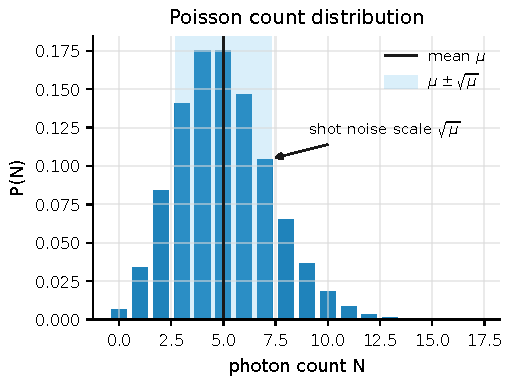
\includegraphics[width=0.85\linewidth]{figures/generated/chapter_01/ch01_photon_count_statistics.pdf}
\caption{泊松计数分布的基本形状（此处取单一平均计数 $\mu$ 作示意）。平均计数为 $\mu$ 时，分布围绕 $\mu$ 铺开，方差也等于 $\mu$，因此涨落的尺度（误差棒）是 $\sqrt{\mu}$，相对散粒噪声为 $1/\sqrt{\mu}$。图中标出了均值线与 $\pm\sqrt{\mu}$ 的涨落带。}
\label{fig:e03-poisson}
\end{figure}

\section{当方差不再等于均值：一个留给后文的问题}
\label{sec:e03-beyond}

现在把整章的逻辑倒过来看一遍。我们得到 $\operatorname{Var}(N)=\mu$，靠的是一个很硬的前提——不同小格里的到达相互独立，从而方差可加（式 \eqref{eq:e03-var-additive}）。这个前提一旦成立，均值和方差就被锁成同一个数。那么反过来：如果有一天你在实验里认认真真地测出方差和均值，发现它们并不相等，这条链子必然是在"独立"这一环断了。

于是"方差比均值大还是小"就成了一个直接读取光子行为的探针。定义一个方便的比值——曼德尔 Q 参数（Mandel $Q$ parameter）——来量化偏离：
\begin{equation}
  Q=\frac{\operatorname{Var}(N)-\mu}{\mu}.
  \label{eq:e03-mandelQ}
\end{equation}
\begin{formulaexplain}
$Q$ 度量计数统计相对泊松的偏离：$Q=0$ 是泊松（独立到达）；$Q>0$ 方差超出均值，称超泊松；$Q<0$ 方差小于均值，称亚泊松。它把"独立不独立"翻成一个可测的数。
\end{formulaexplain}
三种情形对应三幅截然不同的物理画面。$Q=0$，方差等于均值，就是本章的泊松基准，光子彼此不打招呼。$Q>0$，方差鼓出来了，叫超泊松（super-Poissonian）：光子倾向于扎堆到达，一个来了、同伴也更容易结伴而至，仿佛它们爱抱团——这就是聚束（bunching），是热光、星光这类混沌光（chaotic light）的招牌。$Q<0$，方差被压下去了，叫亚泊松（sub-Poissonian）：光子彼此推开，一个刚到、下一个偏偏躲着不来，到达比随机还要"均匀"——这就是反聚束（antibunching），是单光子源等真正非经典光的指纹，经典电磁波无论如何摆弄都做不出来。

把这两幅画面推到极端，就触到本章末尾埋下的那个协方差：聚束意味着相邻时间的到达是正相关的（$\operatorname{Cov}>0$，方差被顶大），反聚束意味着负相关（$\operatorname{Cov}<0$，方差被削小）。度量这种"一个光子到达之后、另一个光子更可能还是更不可能紧跟着到达"的相关强度，需要一个专门的工具——二阶相干函数（second-order coherence）$g^{(2)}(\tau)$。它测的正是"在时刻 $t$ 探测到一个光子的条件下，再过 $\tau$ 又探测到一个光子"的相对概率：$g^{(2)}(0)>1$ 是聚束，$g^{(2)}(0)<1$ 是反聚束，$g^{(2)}=1$ 回到本章这条各处独立的泊松基线。

换句话说，本章把"计数的语言"讲到了它的边界：只要光子独立到达，一切都被 $\mu=R_\gamma\Delta t$ 和 $\operatorname{Var}(N)=\mu$ 两条式子锁定。而真正有趣的天体物理和量子光学，恰恰住在这条边界之外——住在方差偏离均值、光子开始互相"感知"彼此的地方。如何系统地度量这份偏离、它又如何反过来告诉我们光源的物理性质乃至天体的角尺度，是后面专讲二阶相干 $g^{(2)}$ 的章节要展开的正题。到那时你会看到，本章这条不起眼的 $\operatorname{Var}(N)=\mu$，正是整座强度干涉大厦的地基。

\section{本章要点}
\label{sec:e03-summary}

\begin{itemize}
  \item \textbf{四个词。}随机变量给出取每个值的概率（归一化 $\sum P(N)=1$）；期望 $\langle N\rangle$ 永远可加；方差 $\operatorname{Var}(N)=\langle N^2\rangle-\langle N\rangle^2$ 度量涨落；独立性让方差也可加——这是全章最关键的杠杆。
  \item \textbf{平均计数。}一个时间 bin 的平均计数 $\mu=R_\gamma\Delta t$；取 $R_\gamma=10^5\,\mathrm{s^{-1}}$、$\Delta t=1\,\mathrm{ms}$ 得 $\mu=100$。"平均"是许多同条件 bin 的归宿，不是任何一次的实测值。
  \item \textbf{泊松分布。}把 bin 切成 $M$ 个小格、每格点击概率 $p=\mu/M$，计数服从二项分布 \eqref{eq:e03-binomial}；令 $M\to\infty$，用 $\binom{M}{N}p^N\to\mu^N/N!$ 和标准极限 $(1-\mu/M)^M\to e^{-\mu}$，得 $P(N)=e^{-\mu}\mu^N/N!$。
  \item \textbf{散粒噪声。}由小格独立叠加得 $\operatorname{Var}(N)=\mu$；标准差 $\sqrt{\mu}$，相对散粒噪声 $1/\sqrt{\mu}$，信噪比 $\sqrt{\mu}$。$\mu=10^4$ 时相对误差 $1\%$；$\mu=1$ 时计数本身主导。误差减半要多数四倍的光子。
  \item \textbf{边界之外。}方差偏离均值（$Q\neq0$）意味着光子不再独立到达：超泊松对应聚束，亚泊松对应反聚束。度量这份相关的工具是二阶相干函数 $g^{(2)}$，留待后面专讲它的章节展开。
\end{itemize}

\medskip
\noindent\textbf{想一想。}
\begin{enumerate}
  \item 若把 bin 宽度 $\Delta t$ 加倍，$\mu$、$\sigma$、相对噪声 $1/\sqrt{\mu}$ 各自如何变化？信噪比呢？
  \item 一台望远镜每秒探测 $10^6$ 个光子，你想让某个测量的相对散粒噪声达到 $0.1\%$，至少要积分多久（假设纯散粒噪声）？
  \item 假如你测到某个源的方差明显小于均值（$Q<0$），在完全排除仪器问题后，这在物理上意味着什么？经典电磁波能给出这种结果吗？
\end{enumerate}

\chapter{量子力学与谐振子：阶梯算符}
\label{chap:e04}

\begin{chapteropening}
到目前为止，我们一直在说“光子”，却从没认真问过：光子究竟是从哪里冒出来的？它不是一颗事先就藏在真空里的小球，而是某个振动模式的一次“跳级”。要把这句话讲清楚，必须先回到量子力学里最朴素、也最重要的一个系统——谐振子（harmonic oscillator）。

本章的核心问题只有一个：一个来回振动的系统，它的能量为什么只能一格一格地取值？答案藏在两个算符里——一个专门“往下走一格”，一个专门“往上走一格”。它们叫做阶梯算符（ladder operators）。我们会从最普通的位置、动量出发，一步不跳地把这两个算符造出来，证明它们满足一条极其干净的对易关系，再用它们把能量谱、数态、零点能全部一次性读出来。这是整本书里“光子从哪来”的第一块基石：把这一章的代数吃透，后面所有关于相干态、热态、光子统计的讨论都只是它的推广。
\end{chapteropening}

\section{量子力学最小复习}
\label{sec:e04-review}

在动手之前，我们先把后面要反复用到的几件量子力学“工具”摆到桌面上。这一节不做证明，只是把你大概率见过一次的东西重新点亮一下；如果每一条你都觉得眼熟，那正说明你已经准备好了。

\paragraph{态矢量。}
一个量子系统在某一时刻的状态，用一个矢量 \(|\psi\rangle\) 表示，读作“ket psi”。你可以把它想成一支住在抽象空间（希尔伯特空间，Hilbert space）里的箭头。它的对偶伙伴写成 \(\langle\psi|\)（“bra psi”），两者拼起来 \(\langle\psi|\psi\rangle\) 就是这支箭头长度的平方。物理上我们总要求态是归一的：
\[
  \langle\psi|\psi\rangle=1,
\]
因为“系统一定处在某个状态”的总概率必须是 1。

\paragraph{算符与本征值。}
对系统能做的每一个物理测量（能量、位置、动量……），都对应一个算符（operator），我们用带帽子的字母表示，例如 \(\hat H,\hat x,\hat p\)。算符作用在态上会给出一个新态。特别地，如果某个态满足
\[
  \hat A\,|a\rangle = a\,|a\rangle,
\]
就说 \(|a\rangle\) 是 \(\hat A\) 的本征态（eigenstate），数 \(a\) 是对应的本征值（eigenvalue）。物理上，只有当系统正好处在 \(|a\rangle\) 时，测量 \(A\) 才会确定地得到 \(a\)。可观测量对应的算符都是厄米的（Hermitian，\(\hat A^\dagger=\hat A\)），这保证本征值是实数——测出来的数当然得是实的。

\paragraph{期望值。}
如果态不是本征态，测量结果就有涨落，我们只能谈平均值。在态 \(|\psi\rangle\) 上测量 \(A\)，多次重复的平均记为期望值（expectation value）
\begin{equation}
  \langle A\rangle \equiv \langle\psi|\,\hat A\,|\psi\rangle .
  \label{eq:e04-expectation}
\end{equation}
\begin{formulaexplain}
\(\langle A\rangle\) 是可观测量 \(A\) 在态 \(|\psi\rangle\) 上的平均测量值。把算符 \(\hat A\) 夹在 \(\langle\psi|\) 和 \(|\psi\rangle\) 中间即可。态若归一，它就是真正意义上的平均。
\end{formulaexplain}
这里 \(\hat A\) 是待测量对应的算符，\(|\psi\rangle\) 是系统当前的（归一）态。式 \eqref{eq:e04-expectation} 是我们本章反复要用的“提取数值”的唯一手段：一旦知道了态和算符，任何平均量都用它算出来。它没有单位问题——单位完全由 \(\hat A\) 决定，例如 \(\hat A=\hat H\) 时 \(\langle H\rangle\) 是能量（erg）。

\paragraph{对易子。}
两个算符先后作用的顺序一般不能交换，这种“不可交换”正是量子力学与经典力学的根本分野。我们用对易子（commutator）来度量它：
\begin{equation}
  [\hat A,\hat B]\equiv \hat A\hat B-\hat B\hat A .
  \label{eq:e04-commutator}
\end{equation}
\begin{formulaexplain}
\([\hat A,\hat B]\) 衡量“先 \(B\) 后 \(A\)”与“先 \(A\) 后 \(B\)”的差别。若它为零，两个量可以同时被精确测量；若不为零，它们互相“打架”。
\end{formulaexplain}
\(\hat A\hat B\) 表示先让 \(\hat B\) 作用、再让 \(\hat A\) 作用（算符从右往左作用在态上）。若 \([\hat A,\hat B]=0\)，我们说两算符对易，它们有共同的本征态，可以同时有确定值；若不为零，就不能。后面我们造阶梯算符时，几乎每一步化简都是在反复搬动这个 \(\hat A\hat B-\hat B\hat A\)。一条马上要用到的恒等式（直接展开即可验证）是
\[
  [\hat A,\hat B\hat C]=[\hat A,\hat B]\hat C+\hat B[\hat A,\hat C].
\]

\paragraph{正则对易关系。}
在所有对易子里，最基本的一条是位置和动量之间的正则对易关系（canonical commutation relation）：
\begin{equation}
  [\hat x,\hat p]=i\hbar .
  \label{eq:e04-xp}
\end{equation}
\begin{formulaexplain}
\(\hat x\) 是位置算符，\(\hat p\) 是动量算符，\(\hbar\) 是约化普朗克常数。它们不对易，差出一个纯虚常数 \(i\hbar\)。这是整个量子力学的“地基砖”。
\end{formulaexplain}
式 \eqref{eq:e04-xp} 里，\(\hat x\) 的量纲是长度（cm），\(\hat p\) 的量纲是动量（\(\mathrm{g\,cm\,s^{-1}}\)），乘积的量纲是作用量（\(\mathrm{erg\,s}\)），正好与 \(\hbar\) 一致（\(\hbar\simeq1.05\times10^{-27}\,\mathrm{erg\,s}\)）。注意右边是一个纯数乘以单位算符，与态无关——这正是它“基本”的原因。本章后面所有代数，归根到底只用到这一条 \([\hat x,\hat p]=i\hbar\)，其余全是逻辑推演。

\paragraph{测不准关系。}
两个不对易的量不能同时被无限精确地确定，这就是测不准关系（uncertainty relation）。它的一般形式叫罗伯逊不等式（Robertson inequality）：对任意两个厄米算符 \(\hat A,\hat B\)，在任意态上它们的标准差满足
\[
  \Delta A\,\Delta B\ \ge\ \frac12\big|\langle[\hat A,\hat B]\rangle\big| .
\]
这条不等式的右边正是由对易子决定的——两个量越“不对易”，就越无法同时确定。我们不在复习节里证明它，只把它作为已知结果拿来用。现在取 \(\hat A=\hat x,\hat B=\hat p\)，代入正则对易关系 \eqref{eq:e04-xp} 的 \([\hat x,\hat p]=i\hbar\)，右边的期望值 \(\langle i\hbar\rangle=i\hbar\)（它是个纯常数，与态无关），于是 \(\tfrac12|\langle[\hat x,\hat p]\rangle|=\tfrac12|i\hbar|=\hbar/2\)，得到最著名的一条：
\[
  \Delta x\,\Delta p\ \ge\ \frac{\hbar}{2},
\]
其中 \(\Delta x=\sqrt{\langle \hat x^2\rangle-\langle\hat x\rangle^2}\) 是位置的标准差，\(\Delta p\) 类似。它告诉我们：一个量子态不可能同时把位置和动量都压到零涨落。记住这个“最小面积 \(\hbar/2\)”，因为谐振子的基态恰好是把这个不等式取到等号的态——它是量子涨落所能达到的最“安静”的振动。这一节到此为止；我们已经把工具备齐了。

\section{量子谐振子与阶梯算符的构造}
\label{sec:e04-ladder}

现在进入正题。想象一颗小球拴在弹簧上来回振动，或者一个双原子分子里两个原子相对伸缩，或者——这才是我们真正关心的——电磁场里一个单一模式的振荡。它们在数学上是同一个系统：谐振子。在量子力学里，它的哈密顿量（Hamiltonian，即能量算符）是
\begin{equation}
  \hat H=\frac{\hat p^2}{2m}+\frac{1}{2}m\omega^2\hat x^2 .
  \label{eq:e04-hamiltonian}
\end{equation}
\begin{formulaexplain}
第一项 \(\hat p^2/2m\) 是动能，第二项 \(\tfrac12 m\omega^2\hat x^2\) 是弹簧势能。\(m\) 是质量，\(\omega\) 是振动角频率。整条式子就是“动能加势能”的量子版本。
\end{formulaexplain}
式 \eqref{eq:e04-hamiltonian} 里 \(m\) 是质量（g），\(\omega\) 是角频率（\(\mathrm{rad\,s^{-1}}\)），\(\hat x,\hat p\) 是上一节的位置、动量算符。整体量纲是能量（erg）。经典地，这个系统会以频率 \(\omega\) 做正弦振动，能量可以连续取任意正值。量子的问题是：\(\hat H\) 的本征值——也就是允许的能量——长什么样？

直接去解微分方程当然可以，但那样会淹没在特殊函数里。有一条优雅得多的路：把 \(\hat H\) 因式分解。注意 \(\hat p^2/2m+\tfrac12 m\omega^2\hat x^2\) 形状像 \(a^2+b^2\)，而 \(a^2+b^2=(a-ib)(a+ib)\)——只不过 \(\hat x\) 与 \(\hat p\) 不对易，因式分解会留下“尾巴”，那条尾巴恰恰藏着全部物理。为此我们定义两个新算符：
\begin{equation}
  \hat a=\sqrt{\frac{m\omega}{2\hbar}}\left(\hat x+\frac{i\,\hat p}{m\omega}\right),
  \qquad
  \hat a^\dagger=\sqrt{\frac{m\omega}{2\hbar}}\left(\hat x-\frac{i\,\hat p}{m\omega}\right).
  \label{eq:e04-adef}
\end{equation}
\begin{formulaexplain}
\(\hat a\) 是湮灭算符，\(\hat a^\dagger\) 是产生算符，二者互为厄米共轭。它们把有量纲的 \(\hat x,\hat p\) 打包成无量纲的组合，是通向能级阶梯的“钥匙”。
\end{formulaexplain}
先说量纲，确认这两个定义是“干净”的。系数 \(\sqrt{m\omega/2\hbar}\) 的量纲是 \(\sqrt{\mathrm{g}\cdot\mathrm{s^{-1}}/\mathrm{erg\,s}}=\mathrm{cm^{-1}}\)（因为 \(\mathrm{erg}=\mathrm{g\,cm^2\,s^{-2}}\)），乘上量纲为 cm 的 \(\hat x\)，得到一个纯数；而 \(\hat p/(m\omega)\) 的量纲是 \(\mathrm{g\,cm\,s^{-1}}/(\mathrm{g\,s^{-1}})=\mathrm{cm}\)，也乘成纯数。所以 \(\hat a,\hat a^\dagger\) 都是无量纲算符——这很重要，它们数的是“第几格”，本来就不该带单位。因为 \(\hat x,\hat p\) 是厄米算符，把式 \eqref{eq:e04-adef} 取厄米共轭（\(i\to -i\)）立刻看出 \(\hat a\) 与 \(\hat a^\dagger\) 确实互为共轭。

\paragraph{反解出 \(\hat x,\hat p\)。}
定义之后，我们常常需要反过来把 \(\hat x,\hat p\) 用 \(\hat a,\hat a^\dagger\) 表示。把式 \eqref{eq:e04-adef} 两式相加、相减即可：相加时虚部相消，相减时实部相消，
\[
  \hat a+\hat a^\dagger=\sqrt{\frac{m\omega}{2\hbar}}\,(2\hat x),
  \qquad
  \hat a-\hat a^\dagger=\sqrt{\frac{m\omega}{2\hbar}}\,\frac{2i\,\hat p}{m\omega}.
\]
于是
\begin{equation}
  \hat x=\sqrt{\frac{\hbar}{2m\omega}}\,(\hat a+\hat a^\dagger),
  \qquad
  \hat p=-i\sqrt{\frac{m\omega\hbar}{2}}\,(\hat a-\hat a^\dagger).
  \label{eq:e04-xp-in-a}
\end{equation}
\begin{formulaexplain}
把位置和动量重新写成产生、湮灭算符的组合。\(\hat x\) 对应“对称”组合 \(\hat a+\hat a^\dagger\)，\(\hat p\) 对应“反对称”组合 \(\hat a-\hat a^\dagger\)，各自配一个带量纲的前因子。
\end{formulaexplain}
这两条以后会反复用到：任何含 \(\hat x,\hat p\) 的量（比如电场，它正比于 \(\hat x\)）都能翻译成产生、湮灭算符的语言。前因子 \(\sqrt{\hbar/2m\omega}\) 的量纲正好是 cm，\(\sqrt{m\omega\hbar/2}\) 正好是动量单位，量纲自洽。

\paragraph{关键一步：算出 \([\hat a,\hat a^\dagger]\)。}
这是全章最重要的代数，我们一步不跳地做。把定义式 \eqref{eq:e04-adef} 代入对易子，先把常数系数 \(m\omega/2\hbar\) 提到前面：
\[
  [\hat a,\hat a^\dagger]
  =\frac{m\omega}{2\hbar}
  \left[\hat x+\frac{i\hat p}{m\omega},\ \hat x-\frac{i\hat p}{m\omega}\right].
\]
对易子对两边都是线性的，把它按四项展开：
\[
  \left[\hat x+\tfrac{i\hat p}{m\omega},\ \hat x-\tfrac{i\hat p}{m\omega}\right]
  =[\hat x,\hat x]
  -\frac{i}{m\omega}[\hat x,\hat p]
  +\frac{i}{m\omega}[\hat p,\hat x]
  -\frac{i^2}{(m\omega)^2}[\hat p,\hat p].
\]
现在逐项处理。任何算符和自己对易，所以 \([\hat x,\hat x]=[\hat p,\hat p]=0\)，第一项和第四项直接消失。中间两项用正则对易关系 \eqref{eq:e04-xp}：\([\hat x,\hat p]=i\hbar\)，而 \([\hat p,\hat x]=-[\hat x,\hat p]=-i\hbar\)。代入：
\[
  =-\frac{i}{m\omega}(i\hbar)+\frac{i}{m\omega}(-i\hbar)
  =-\frac{i^2\hbar}{m\omega}-\frac{i^2\hbar}{m\omega}
  =\frac{\hbar}{m\omega}+\frac{\hbar}{m\omega}
  =\frac{2\hbar}{m\omega},
\]
这里用了 \(i^2=-1\)。把它乘回前面的系数：
\[
  [\hat a,\hat a^\dagger]=\frac{m\omega}{2\hbar}\cdot\frac{2\hbar}{m\omega}=1.
\]
于是我们得到本章的“主定理”：
\begin{equation}
  [\hat a,\hat a^\dagger]=1 .
  \label{eq:e04-aacomm}
\end{equation}
\begin{formulaexplain}
产生与湮灭算符的对易子等于 1。这条极简的关系是谐振子（以及后面每一个光场模式）全部量子结构的源头，能级、光子、零点能都从它长出来。
\end{formulaexplain}
请体会这条式子有多干净：有量纲的 \(\hat x,\hat p\)、有单位的 \(m,\omega,\hbar\) 全部约掉，只剩一个赤裸裸的 1。它无量纲，与具体是哪种振子无关。式 \eqref{eq:e04-aacomm} 会成为我们唯一需要记住的对易关系——从这一刻起，我们几乎可以把 \(\hat x,\hat p\) 忘掉，只在 \(\hat a,\hat a^\dagger\) 的代数里工作。作为对比，产生算符之间、湮灭算符之间当然对易：\([\hat a,\hat a]=[\hat a^\dagger,\hat a^\dagger]=0\)。

\section{用数算符改写哈密顿量}
\label{sec:e04-numberH}

造出 \(\hat a,\hat a^\dagger\) 是为了简化 \(\hat H\)。现在我们把式 \eqref{eq:e04-hamiltonian} 翻译成产生、湮灭算符的语言。最省事的做法是先算组合 \(\hat a^\dagger\hat a\)，看看它离 \(\hat H\) 有多远。用定义 \eqref{eq:e04-adef}，把系数提出：
\[
  \hat a^\dagger\hat a
  =\frac{m\omega}{2\hbar}
  \left(\hat x-\frac{i\hat p}{m\omega}\right)\!\left(\hat x+\frac{i\hat p}{m\omega}\right).
\]
小心地把括号乘开（注意保持算符顺序，因为它们不对易）：
\[
  \left(\hat x-\tfrac{i\hat p}{m\omega}\right)\!\left(\hat x+\tfrac{i\hat p}{m\omega}\right)
  =\hat x^2+\frac{i}{m\omega}\hat x\hat p-\frac{i}{m\omega}\hat p\hat x-\frac{i^2}{(m\omega)^2}\hat p^2 .
\]
把中间两项合起来，它们正是一个对易子：\(\dfrac{i}{m\omega}(\hat x\hat p-\hat p\hat x)=\dfrac{i}{m\omega}[\hat x,\hat p]=\dfrac{i}{m\omega}(i\hbar)=-\dfrac{\hbar}{m\omega}\)。而最后一项 \(-i^2\hat p^2/(m\omega)^2=+\hat p^2/(m\omega)^2\)。于是
\[
  \hat a^\dagger\hat a
  =\frac{m\omega}{2\hbar}
  \left(\hat x^2+\frac{\hat p^2}{(m\omega)^2}-\frac{\hbar}{m\omega}\right)
  =\frac{m\omega}{2\hbar}\hat x^2+\frac{1}{2\hbar m\omega}\hat p^2-\frac12 .
\]
把前两项各乘一个 \(\hbar\omega\) 看它们是不是 \(\hat H\)：
\[
  \hbar\omega\left(\frac{m\omega}{2\hbar}\hat x^2\right)=\frac12 m\omega^2\hat x^2,
  \qquad
  \hbar\omega\left(\frac{1}{2\hbar m\omega}\hat p^2\right)=\frac{\hat p^2}{2m}.
\]
这正好是式 \eqref{eq:e04-hamiltonian} 的势能项和动能项！所以 \(\hbar\omega\,\hat a^\dagger\hat a=\hat H-\tfrac12\hbar\omega\)，整理即得
\begin{equation}
  \hat H=\hbar\omega\left(\hat a^\dagger\hat a+\frac12\right)
        =\hbar\omega\left(\hat n+\frac12\right),
  \qquad \hat n\equiv\hat a^\dagger\hat a .
  \label{eq:e04-Hn}
\end{equation}
\begin{formulaexplain}
哈密顿量被写成数算符 \(\hat n=\hat a^\dagger\hat a\) 的简单线性函数。能量等于“激发格数 \(\hat n\) 加上半格”再乘以 \(\hbar\omega\)。那半格就是零点能。
\end{formulaexplain}
这里 \(\hat n=\hat a^\dagger\hat a\) 叫数算符（number operator），它是厄米的（\((\hat a^\dagger\hat a)^\dagger=\hat a^\dagger\hat a\)），因此有实本征值——我们马上会看到它的本征值恰好是 \(0,1,2,\ldots\)，也就是“这个模式里有几个量子”。式 \eqref{eq:e04-Hn} 把求能谱的问题彻底简化：只要知道 \(\hat n\) 的本征值，能量就读出来了。量纲上，\(\hat n\) 无量纲，\(\hbar\omega\) 是能量，一切自洽。

\paragraph{零点能。}
式 \eqref{eq:e04-Hn} 里那个 \(+\tfrac12\) 不是可有可无的常数。即使 \(\hat n\) 取最小值 0，能量也不是零，而是
\[
  E_0=\frac12\hbar\omega .
\]
这就是零点能（zero-point energy）。物理上它是测不准关系的直接后果：如果振子真的静止在势阱底部，那它就同时有了确定的位置（\(x=0\)）和确定的动量（\(p=0\)），违反 \(\Delta x\,\Delta p\ge\hbar/2\)。量子力学不允许这种“绝对的安静”，于是即便在基态，振子也必须保有一份最低限度的抖动，对应能量 \(\tfrac12\hbar\omega\)。这份抖动不是我们测量能力的不足，而是真空本身的性质——后面讲光场时，正是这份“真空涨落”给出散粒噪声与压缩态的物理起点。给个数量级：可见光一个模式 \(\nu\sim6\times10^{14}\,\mathrm{Hz}\)，\(\hbar\omega=h\nu\simeq(6.6\times10^{-27})(6\times10^{14})\,\mathrm{erg}\simeq4\times10^{-12}\,\mathrm{erg}\approx2.5\,\mathrm{eV}\)，零点能约 1.2 eV——一个绝非可以忽略的量。

\section{数态：能量的一格一格}
\label{sec:e04-numberstates}

现在来读能谱。由式 \eqref{eq:e04-Hn}，\(\hat H\) 和 \(\hat n\) 只差一个常数和一个正因子，它们共享本征态。设 \(\hat n\) 的本征态为 \(|n\rangle\)，本征值为 \(n\)：
\[
  \hat n\,|n\rangle=n\,|n\rangle .
\]
我们把 \(|n\rangle\) 叫数态或福克态（number state / Fock state）。眼下 \(n\) 还只是一个待定的实数；这一节的任务，就是用对易关系 \eqref{eq:e04-aacomm} 逼出它只能是非负整数，并顺便求出 \(\hat a,\hat a^\dagger\) 作用在 \(|n\rangle\) 上到底给出什么。

\paragraph{阶梯算符为什么“爬楼梯”。}
先算两条关键的对易子。用 \([\hat a,\hat a^\dagger]=1\)：
\[
  [\hat n,\hat a]=[\hat a^\dagger\hat a,\hat a]
  =\hat a^\dagger[\hat a,\hat a]+[\hat a^\dagger,\hat a]\hat a
  =0+(-1)\hat a=-\hat a,
\]
其中用了展开恒等式 \([\hat A\hat B,\hat C]=\hat A[\hat B,\hat C]+[\hat A,\hat C]\hat B\) 以及 \([\hat a^\dagger,\hat a]=-1\)。同理
\[
  [\hat n,\hat a^\dagger]=\hat a^\dagger[\hat a,\hat a^\dagger]+[\hat a^\dagger,\hat a^\dagger]\hat a
  =\hat a^\dagger(1)+0=+\hat a^\dagger .
\]
这两条 \([\hat n,\hat a]=-\hat a\)、\([\hat n,\hat a^\dagger]=+\hat a^\dagger\) 就是“阶梯”的机械原理。看它们如何起作用：把 \(\hat n\) 作用在新态 \(\hat a|n\rangle\) 上，
\[
  \hat n\,(\hat a|n\rangle)
  =(\hat a\hat n+[\hat n,\hat a])|n\rangle
  =(\hat a\hat n-\hat a)|n\rangle
  =\hat a(\hat n-1)|n\rangle
  =(n-1)\,\hat a|n\rangle .
\]
读这行字：\(\hat a|n\rangle\) 又是 \(\hat n\) 的本征态，本征值降了 1，变成 \(n-1\)。所以 \(\hat a\) 把系统“往下带一格”，这就是它被叫做湮灭算符（annihilation operator）的原因。完全对称地，
\[
  \hat n\,(\hat a^\dagger|n\rangle)=(n+1)\,\hat a^\dagger|n\rangle,
\]
\(\hat a^\dagger\) 把系统“往上抬一格”，是产生算符（creation operator）。这就是“阶梯”二字的来历。

\paragraph{阶梯必须有底：\(n\) 是非负整数。}
为什么台阶不能无限往下延伸到负数？因为 \(\hat n\) 的本征值不可能为负。用式 \eqref{eq:e04-expectation}，对归一的 \(|n\rangle\) 算 \(\hat n\) 的期望值：
\[
  n=\langle n|\hat n|n\rangle=\langle n|\hat a^\dagger\hat a|n\rangle
  =\big(\hat a|n\rangle\big)^\dagger\big(\hat a|n\rangle\big)
  =\big\|\,\hat a|n\rangle\,\big\|^2\ \ge 0 .
\]
关键就在中间这步：\(\langle n|\hat a^\dagger\hat a|n\rangle\) 是态 \(\hat a|n\rangle\) 与自己的内积，也就是它长度的平方，而任何矢量长度的平方都非负。所以 \(n\ge0\)。可是 \(\hat a\) 每作用一次就把本征值减 1，若从某个非整数的 \(n\) 出发反复作用 \(\hat a\)，迟早会跌破 0，得到一个负本征值——矛盾。唯一的出路是：这串下降必须在某一步正好落到 0 然后停住，也就是存在一个基态 \(|0\rangle\) 满足
\begin{equation}
  \hat a\,|0\rangle=0 .
  \label{eq:e04-ground}
\end{equation}
\begin{formulaexplain}
湮灭算符作用在基态上给出零（不是态 \(|0\rangle\)，而是零矢量）。这表示“已经到最底层，再往下没有台阶了”。基态是整座能量阶梯的地板。
\end{formulaexplain}
只有当下降序列在 \(n=0\) 处被式 \eqref{eq:e04-ground} 掐断，才不会出现负本征值。由此倒推：从 \(|0\rangle\) 一步步用 \(\hat a^\dagger\) 往上爬，得到的本征值只能是 \(0,1,2,3,\ldots\)。换句话说，谐振子的激发数只能是非负整数——这正是“光子只能一个一个地有”的数学根源。

\paragraph{归一化系数：那两个 \(\sqrt{\ }\) 从哪来。}
我们已知 \(\hat a|n\rangle\) 正比于 \(|n-1\rangle\)，但比例常数是多少？这一步必须算全，因为后面光子统计里的因子全靠它。设 \(\hat a|n\rangle=c_n|n-1\rangle\)，其中 \(c_n\) 是待定常数，且 \(|n-1\rangle\) 已归一。两边取模平方：
\[
  \big\|\hat a|n\rangle\big\|^2
  =|c_n|^2\,\langle n-1|n-1\rangle
  =|c_n|^2 .
\]
而左边我们刚算过：\(\big\|\hat a|n\rangle\big\|^2=\langle n|\hat a^\dagger\hat a|n\rangle=\langle n|\hat n|n\rangle=n\)。所以 \(|c_n|^2=n\)，取正实的相位约定得 \(c_n=\sqrt{n}\)。完全类似地，为求 \(\hat a^\dagger|n\rangle=d_n|n+1\rangle\)，我们需要 \(\hat a\hat a^\dagger\) 的作用；由 \eqref{eq:e04-aacomm}，\(\hat a\hat a^\dagger=\hat a^\dagger\hat a+1=\hat n+1\)，于是
\[
  \big\|\hat a^\dagger|n\rangle\big\|^2
  =\langle n|\hat a\hat a^\dagger|n\rangle
  =\langle n|(\hat n+1)|n\rangle
  =n+1
  =|d_n|^2,
\]
给出 \(d_n=\sqrt{n+1}\)。把两条结论并排写出：
\begin{equation}
  \hat a\,|n\rangle=\sqrt{n}\,|n-1\rangle,
  \qquad
  \hat a^\dagger\,|n\rangle=\sqrt{n+1}\,|n+1\rangle .
  \label{eq:e04-ladder-action}
\end{equation}
\begin{formulaexplain}
湮灭算符把 \(|n\rangle\) 降到 \(|n-1\rangle\)，带系数 \(\sqrt{n}\)；产生算符把它升到 \(|n+1\rangle\)，带系数 \(\sqrt{n+1}\)。这两个平方根因子在后面所有光子计数公式里都会露面。
\end{formulaexplain}
注意两个细节。其一，当 \(n=0\) 时 \(\sqrt{n}=0\)，第一式自动退化成 \(\hat a|0\rangle=0\)，与式 \eqref{eq:e04-ground} 一致——地板确实封住了。其二，系数不是简单的 1，而是 \(\sqrt n\) 和 \(\sqrt{n+1}\)：正是这种“越高的台阶，跨步越大”的非线性，让相干态和热态的光子统计呈现出各自独特的形状。式 \eqref{eq:e04-ladder-action} 也给出构造任意数态的配方：反复用 \(\hat a^\dagger\) 从基态往上搭，
\[
  |n\rangle=\frac{(\hat a^\dagger)^n}{\sqrt{n!}}\,|0\rangle,
\]
其中 \(\sqrt{n!}\) 正是把一路上的 \(\sqrt{1}\cdot\sqrt{2}\cdots\sqrt{n}\) 累乘起来的结果。

\paragraph{能级：等间距的梯子。}
把 \(\hat n|n\rangle=n|n\rangle\) 代回式 \eqref{eq:e04-Hn}，能量本征值立刻读出：
\begin{equation}
  E_n=\hbar\omega\left(n+\frac12\right),\qquad n=0,1,2,\ldots
  \label{eq:e04-energy}
\end{equation}
\begin{formulaexplain}
第 \(n\) 个能级的能量。相邻能级间隔恒为 \(\hbar\omega\)，最低能级不是 0 而是 \(\tfrac12\hbar\omega\)。整座能谱是一把均匀的梯子，底座抬高了半格。
\end{formulaexplain}
式 \eqref{eq:e04-energy} 是本章的收获总账。它有两个鲜明特征。第一，能级是离散的、等间距的：相邻两级永远差 \(E_{n+1}-E_n=\hbar\omega\)，不多不少。正因为这份“恒定的一格”，我们才能干脆地说“吸收一个 \(\hbar\omega\) 的量子就上一层，放出一个就下一层”——这一个量子，对电磁场模式而言就是一个光子。落到真实数量级看看这“一格”有多大：一个典型双原子分子的伸缩振动 \(\omega/2\pi\sim10^{13}\text{--}10^{14}\,\mathrm{Hz}\)（红外波段），相邻能级间隔 \(\hbar\omega\sim0.1\text{--}0.5\,\mathrm{eV}\)，正好是红外光谱线的能量；而我们真正关心的可见光单模，\(\nu\sim6\times10^{14}\,\mathrm{Hz}\)，一格就是 \(\hbar\omega\approx2.5\,\mathrm{eV}\)，恰是一个可见光光子的能量。同一把梯子，换个 \(\omega\) 就从分子振动跨到光场。第二，底座被零点能抬到了 \(\tfrac12\hbar\omega\)，如上一节所述。把 \(E_n\) 画出来，就是一把从 \(\tfrac12\hbar\omega\) 起步、每级升高 \(\hbar\omega\) 的等距梯子；数态 \(|n\rangle\) 就是站在第 \(n\) 级上的态，携带 \(n\) 个能量量子。到这里，”光子从哪来”这个问题在单个模式上已经有了完整答案：光子就是谐振子能量阶梯上的一格激发，\(\hat a^\dagger\) 生出它，\(\hat a\) 湮灭它。图~\ref{fig:e04-energy-ladder} 把这把”梯子”整个画了出来。

\begin{figure}[tbp]
\centering
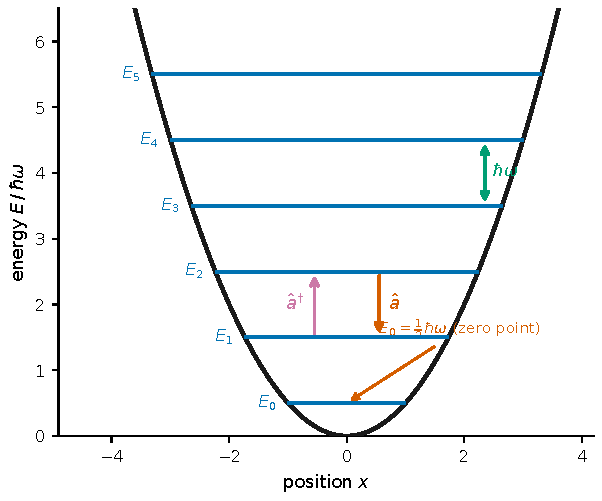
\includegraphics[width=0.6\linewidth]{figures/generated/edu_ch04/e04_energy_ladder.pdf}
\caption{量子谐振子的能量阶梯。在势阱 \(V(x)=\tfrac12 m\omega^2 x^2\) 里，允许的能量只能取等间距的一格一格 \(E_n=\hbar\omega(n+\tfrac12)\)：相邻两级永远相差 \(\hbar\omega\)（绿色双箭头），最低一级不是零，而是零点能 \(\tfrac12\hbar\omega\)（橙色）。产生算符 \(\hat a^\dagger\) 把系统抬高一格、湮灭算符 \(\hat a\) 压低一格。这”恒定的一格” \(\hbar\omega\)，对一个电磁场模式而言，就是一个光子的能量。}
\label{fig:e04-energy-ladder}
\end{figure}

\section{预告：最接近经典振动的量子态}
\label{sec:e04-coherent}

数态 \(|n\rangle\) 能量最确定，却也最“不像”经典振动。想想看：一个经典振子的位置随时间画出漂亮的正弦曲线 \(x(t)=x_0\cos\omega t\)，可数态的位置期望值 \(\langle n|\hat x|n\rangle\) 恒等于零——用式 \eqref{eq:e04-xp-in-a}，\(\hat x\propto\hat a+\hat a^\dagger\) 只会把 \(|n\rangle\) 变成 \(|n\pm1\rangle\)，与 \(\langle n|\) 正交，内积为零。也就是说，一个能量确定的量子振子，位置期望值根本不摆动，它在相空间里是一圈均匀模糊的环，完全没有“此刻在哪一侧”的信息。这与我们对“振动”的日常直觉正好相反。

那么，哪一种量子态才最像经典的来回摆动？答案是相干态（coherent state）\(|\alpha\rangle\)，它被定义为湮灭算符的本征态：
\begin{equation}
  \hat a\,|\alpha\rangle=\alpha\,|\alpha\rangle,\qquad \alpha\in\mathbb{C}.
  \label{eq:e04-coherent}
\end{equation}
\begin{formulaexplain}
相干态是湮灭算符 \(\hat a\) 的本征态，本征值 \(\alpha\) 是一个复数。复数的模给出平均光子数、幅角给出振动相位。它是“最接近经典”的量子态。
\end{formulaexplain}
这个定义初看很奇怪——\(\hat a\) 不是厄米算符，本征值 \(\alpha\) 允许是复数。但正是这个复数替我们同时编码了振幅和相位：\(|\alpha|\) 决定振动多强（可以证明平均光子数 \(\langle\hat n\rangle=|\alpha|^2\)），\(\arg\alpha\) 决定此刻摆到了哪个相位。可以证明，相干态的位置期望值确实随时间做正弦振动，而且它把位置与动量的联合涨落压到测不准关系允许的最小值——它是一团大小恒定、随时间沿圆周匀速平移的小“光斑”，看上去就像一个带着量子模糊的经典点。

不妨在脑子里把这两种态画到同一张“相空间”地图上（横轴是位置 \(x\)，纵轴是动量 \(p\)）。数态 \(|n\rangle\) 的图像是一整圈均匀模糊的环：它的能量（半径的平方）确定，可位置和动量的期望值都恒为零，相位完全不定——你说不出这一刻它“摆到了圆周上的哪一点”，因为它同时糊在整圈上。相干态 \(|\alpha\rangle\) 的图像则是钉在圆周某一点上的一小团紧凑光斑：它有确定的中心，中心到原点的距离约为 \(|\alpha|\)、方位角就是相位 \(\arg\alpha\)，而这团光斑会随时间沿着那个圆周匀速转圈，正好复现出经典正弦振动 \(x(t)\propto\cos\omega t\)。一句话记住二者的差别：数态是”摊平成一整圈的环”，相干态是”凝成一点、绕圈平移的斑”。图~\ref{fig:e04-phase-space} 把这两幅相空间图并排画了出来。

\begin{figure}[tbp]
\centering
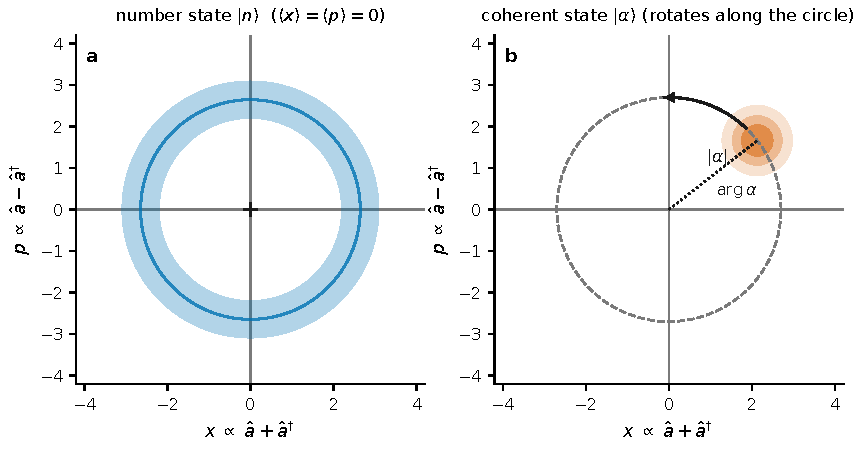
\includegraphics[width=0.92\linewidth]{figures/generated/edu_ch04/e04_phase_space_states.pdf}
\caption{相空间里两种极端量子态（横轴 \(x\propto\hat a+\hat a^\dagger\)，纵轴 \(p\propto\hat a-\hat a^\dagger\)）。左：数态 \(|n\rangle\) 的能量确定（环半径的平方固定），却把概率均匀地摊在整整一圈上，位置和动量的期望都为零、相位完全不定，像一枚模糊的圆环。右：相干态 \(|\alpha\rangle\) 凝成一小团紧凑光斑，钉在半径约 \(|\alpha|\)、方位角为 \(\arg\alpha\) 的圆周上，并沿圆周匀速旋转，复现出经典的正弦振动。}
\label{fig:e04-phase-space}
\end{figure}

这里我们只把定义 \eqref{eq:e04-coherent} 摆出来、给个直觉，具体展开——它的光子数服从泊松分布、它如何写成数态的叠加、它为什么是激光和恒星热光的自然出发点——留到第 \ref{chap:e06} 章。你只需记住一句话：数态是“能量最确定、相位最模糊”的极端，相干态是“相位最清晰、最像经典摆动”的对立极端，而它们用的是同一套 \(\hat a,\hat a^\dagger\)。

\section{本章要点}
\label{sec:e04-summary}

\begin{itemize}
  \item 谐振子的全部量子结构，只需要一条正则对易关系 \([\hat x,\hat p]=i\hbar\)。由它出发定义 \(\hat a,\hat a^\dagger\)（式 \eqref{eq:e04-adef}），逐项计算即得核心关系 \([\hat a,\hat a^\dagger]=1\)（式 \eqref{eq:e04-aacomm}），此后可以只在 \(\hat a,\hat a^\dagger\) 的代数里工作。
  \item 哈密顿量被改写成 \(\hat H=\hbar\omega(\hat n+\tfrac12)\)，其中数算符 \(\hat n=\hat a^\dagger\hat a\)。那个 \(+\tfrac12\) 是零点能 \(\tfrac12\hbar\omega\)，是测不准关系不允许振子绝对静止的直接后果。
  \item 用 \([\hat n,\hat a]=-\hat a\)、\([\hat n,\hat a^\dagger]=+\hat a^\dagger\) 证明 \(\hat a,\hat a^\dagger\) 逐级降/升本征值；用 \(\langle n|\hat a^\dagger\hat a|n\rangle=n\ge0\) 逼出本征值必为非负整数，阶梯在 \(\hat a|0\rangle=0\) 处封底。
  \item 归一化给出 \(\hat a|n\rangle=\sqrt{n}\,|n-1\rangle\)、\(\hat a^\dagger|n\rangle=\sqrt{n+1}\,|n+1\rangle\)，能谱是等间距梯子 \(E_n=\hbar\omega(n+\tfrac12)\)。相邻能级间隔 \(\hbar\omega\) 就是“一个光子”的能量。
  \item 数态是能量最确定、相位最模糊的态；相干态 \(|\alpha\rangle\)（\(\hat a|\alpha\rangle=\alpha|\alpha\rangle\)）则最接近经典振动，详见第 \ref{chap:e06} 章。
\end{itemize}

\paragraph{想一想。}
\begin{itemize}
  \item 如果把 \([\hat x,\hat p]=i\hbar\) 换成经典的 \([\hat x,\hat p]=0\)，重走一遍推导，你会发现 \([\hat a,\hat a^\dagger]\) 变成什么？能级还会离散吗？这说明离散能级到底是谁的功劳。
  \item 数态 \(|n\rangle\) 的位置期望值 \(\langle\hat x\rangle=0\)，但 \(\langle\hat x^2\rangle\) 却随 \(n\) 增大。试用式 \eqref{eq:e04-xp-in-a} 和式 \eqref{eq:e04-ladder-action} 算出 \(\langle n|\hat x^2|n\rangle\)，看看它是不是正比于 \((n+\tfrac12)\)——并解释这个结果和零点能的联系。
  \item 为什么说“吸收一个 \(\hbar\omega\) 的量子”对电磁场就是“多一个光子”？把谐振子的能量阶梯和光子数联系起来，用你自己的话讲一遍。
\end{itemize}

\chapter{光的量子化：从模式到光子}
\label{chap:e05}

\begin{chapteropening}
上一章我们把一个孤立的谐振子（harmonic oscillator）量子化了：能量只能一份一份地取，湮灭算符 \(\hat a\) 拿走一份能量，产生算符 \(\hat a^\dagger\) 添上一份。可那只是一个"弹簧"。真实望远镜面对的是充满整个空间、有颜色、有方向、有偏振、随时间起伏的电磁场。本章要做的，是把第 \ref{chap:e04} 章那一个谐振子的成功，成千上万倍地复制到整个光场上——办法只有一步：把光场先拆成一组"模式"（mode），然后惊讶地发现，每一个模式在数学上就是一个谐振子。于是"光子"这个词第一次获得精确定义：它不是一颗小球，而是某一个模式的一次激发。走完这一章，你会明白望远镜记录的每一次"点击"到底属于什么，也会算出一件反直觉的事：太阳那么亮，可每个光学模式里平均还不到百分之一个光子。
\end{chapteropening}

\section{为什么要把光场拆成"模式"}
\label{sec:e05-why-modes}

先问一个朴素的问题：电磁场是弥漫在整个空间的连续的东西，一个望远镜某一瞬间收到的是一大团振荡的场。我们要怎样把它"数成一份一份"？

答案的关键，是不要一上来就盯着"空间某点某时刻的场强"这种连续量，而是换一组更聪明的坐标。回忆第 \ref{chap:e02} 章的傅里叶分析（Fourier analysis）：任何一段复杂的声波，都可以唯一地写成一堆"纯音"（单一频率的正弦波）的叠加。纯音是声音世界里最简单、彼此独立的"积木"。**模式，就是电磁场版本的"广义纯音"。**

一个电磁场的模式，是一个同时被下面几件事标定的"积木"：

\begin{itemize}
  \item \textbf{频率}\(\ \omega\)（或颜色 \(\nu=\omega/2\pi\)）：这一块积木以多快的节奏振荡；
  \item \textbf{空间形状}\ \(u(\bm r)\)：这一块积木在空间里长什么样——是一束沿某方向传播的平面波，还是一个衍射受限的光斑，或是一根光纤里的导模；
  \item \textbf{偏振}（polarization）：电场矢量在垂直传播方向的平面里指向哪——水平、竖直，或某种旋转；
  \item \textbf{时间窗}\ \(\Delta t\)：这一块积木被"开着"的那段时间。
\end{itemize}

之所以要费劲选这样一组积木，是因为我们希望它们\emph{彼此正交、互不干扰}。正交（orthogonal）的意思和傅里叶里"不同频率的纯音相互独立"完全一样：把场沿这组模式展开，每个模式的系数可以单独测量、单独演化、单独量子化，不会互相牵扯。数学上，一组模式函数 \(\{u_k(\bm r)\}\) 满足正交归一
\[
  \int u_i^*(\bm r)\,u_j(\bm r)\,\mathrm d^3r=\delta_{ij},
\]
其中 \(\delta_{ij}\) 是克罗内克符号（Kronecker delta，\(i=j\) 时为 1，否则为 0）。有了这样一组"广义纯音"，麦克斯韦方程组允许我们把整个电磁场写成
\[
  \bm E(\bm r,t)=\sum_k\big[\,(\text{第 }k\text{ 个模式的振幅})\times u_k(\bm r)\,e^{-i\omega_k t}+\text{复共轭}\,\big].
\]
每一项都在以自己的频率 \(\omega_k\) 独立地振荡——这正是一个"广义纯音"应有的样子。下一节我们就盯住其中任意一个 \(k\)，看看它的振幅遵守什么运动方程。

\section{关键一步：每个模式就是一个谐振子}
\label{sec:e05-mode-is-oscillator}

现在把注意力锁定在单独一个模式 \(k\) 上。它的空间形状 \(u_k(\bm r)\) 是固定的，唯一还在动的，是它的振幅——记作 \(q_k(t)\)。我们要做的，是把这个单模式的场代进电磁场的能量密度、对空间积分，看它携带的总能量长什么样。这一步在标准电动力学里叫"场能量的模式展开"，很多教材（如 Jackson《经典电动力学》讲腔模的一节，或任意一本量子光学入门书的第一章）都会做；但它正是本章的\emph{地基}，跳过去自学读者就无法自证，所以我们把这段代数原原本本走一遍。真正要用到的只有三个事实，我们边走边点名。

\textbf{事实一：电磁场能量密度公式。}自由电磁场装在体积里的总能量是（CGS 单位）
\[
  U=\frac{1}{8\pi}\int\big(\bm E^2+\bm B^2\big)\,\mathrm d^3r,
\]
电场项和磁场项对称地各出一半——这是普通物理电磁学里就学过的结果，单位是 erg。

\textbf{事实二：单模式的场怎么写。}把式子里只保留第 \(k\) 个模式。取它是实驻波（腔模），电场可写成"空间形状 \(\times\) 随时间起伏的振幅"：
\[
  \bm E_k(\bm r,t)=-\,c_1\,\dot q_k(t)\,\bm u_k(\bm r),
\]
其中 \(\bm u_k\) 是上一节那个正交归一的模式函数、\(q_k(t)\) 是我们要盯住的振幅坐标，\(c_1\) 是一个只含常数（\(4\pi\)、\(c\) 等）的比例因子——先带着它，最后会被 \(q_k\) 的定义吸收掉。

\textbf{事实三：麦克斯韦方程把 \(\dot{\bm E}\) 和 \(\bm B\) 拴在一起。}真空里 \(\nabla\times\bm B=\tfrac1c\,\partial_t\bm E\)，所以磁场由电场的时间导数决定。把事实二的 \(\bm E_k\propto\dot q_k\,\bm u_k\) 代进去，右边 \(\propto\ddot q_k\,\bm u_k\)；对以 \(\omega_k\) 简谐振荡的模式 \(\ddot q_k=-\omega_k^2 q_k\)，于是磁场随时间的部分正比于 \(q_k(t)\) 本身，空间部分则由 \(\nabla\times\bm u_k\) 决定：
\[
  \bm B_k(\bm r,t)=c_2\,q_k(t)\,\big[\nabla\times\bm u_k(\bm r)\big].
\]
这里模式还满足亥姆霍兹方程 \(\nabla^2\bm u_k=-(\omega_k^2/c^2)\,\bm u_k\)——"空间形状的弯曲程度定出频率"——它待会儿会帮我们把磁场项的空间积分算成一个含 \(\omega_k^2\) 的数。

现在把事实二、三代进事实一的积分。电场项给出
\[
  \frac1{8\pi}\int\bm E_k^2\,\mathrm d^3r
  =\frac{c_1^2}{8\pi}\,\dot q_k^{\,2}\int|\bm u_k|^2\,\mathrm d^3r
  =\frac{c_1^2}{8\pi}\,\dot q_k^{\,2},
\]
最后一步正是用了上一节的\emph{正交归一} \(\int|\bm u_k|^2\,\mathrm d^3r=1\)，一下把空间积分做成了 1。同样地，磁场项里做同一个积分（用 \(\int|\nabla\times\bm u_k|^2\,\mathrm d^3r=(\omega_k^2/c^2)\int|\bm u_k|^2\,\mathrm d^3r=\omega_k^2/c^2\)，这一步用的就是亥姆霍兹方程）给出
\[
  \frac1{8\pi}\int\bm B_k^2\,\mathrm d^3r
  =\frac{c_2^2}{8\pi}\,q_k^{\,2}\cdot\frac{\omega_k^2}{c^2}
  \ \propto\ \omega_k^2\,q_k^{\,2}.
\]
于是电场项 \(\propto\dot q_k^{\,2}\)、磁场项 \(\propto\omega_k^2 q_k^{\,2}\)，两项一拼，能量就长成了"动能 + 势能"的谐振子模样：
\[
  U_k=(\text{常数}_1)\,\dot q_k^{\,2}+(\text{常数}_2)\,\omega_k^2\,q_k^{\,2}.
\]
最后一步是关键：那两个常数（都由 \(c_1,c_2,4\pi,c\) 等拼成）\emph{不是无关紧要的}。我们\textbf{把 \(q_k\) 重新定义}，让它把这些常数一并吸收进去（这在物理上总能做到：给振幅乘一个常数因子而已）。选好这个归一化，就是把 \(q_k\) 定义成这个模式的\emph{正则坐标}（canonical coordinate），等效质量取成 1。此时两项系数恰好都变成 \(\tfrac12\)，能量正好等于
\[
  H_k=\tfrac12\,\dot q_k^{\,2}+\tfrac12\,\omega_k^2\,q_k^{\,2}.
\]
把这行字读三遍。它和第 \ref{chap:e04} 章那个质量为 1 的弹簧的能量 \(H=\tfrac12\dot q^2+\tfrac12\omega^2 q^2\) \emph{一模一样}——注意这里是精确的\emph{等号}，而不是"正比于"：那个曾经含糊的比例常数，已经被我们对 \(q_k\) 的定义吃掉了，所以等效质量正好是 1 而不是别的系数。也就是说：

\begin{quote}
\textbf{每一个电磁场模式，在数学上就是一个频率为 \(\omega_k\) 的谐振子。}
\end{quote}

这是全章的枢纽。一旦承认这句话，我们就\emph{什么新东西都不用发明}——直接把第 \ref{chap:e04} 章对谐振子做过的量子化，逐字套到每个模式上。第 \ref{chap:e04} 章我们把 \(q,\dot q\) 打包成湮灭算符 \(\hat a\) 与产生算符 \(\hat a^\dagger\)。这里对第 \(k\) 个模式照做，得到一对 \(\hat a_k,\hat a_k^\dagger\)。因为不同模式彼此正交、互不干扰，它们的算符对易关系是

\begin{equation}
  [\hat a_i,\hat a_j^\dagger]=\delta_{ij},\qquad
  [\hat a_i,\hat a_j]=0,\qquad
  \hat n_k=\hat a_k^\dagger\hat a_k .
  \label{eq:e05-commutator}
\end{equation}
\begin{formulaexplain}
\(\hat a_k^\dagger,\hat a_k\) 在第 \(k\) 个模式里加一个、减一个光子；\(\delta_{ij}\) 说明只有\emph{同一个}模式的产生与湮灭才留下量子修正，不同模式完全独立；\(\hat n_k\) 数第 \(k\) 个模式里有几个光子。
\end{formulaexplain}

逐个交代记号。\(\hat a_k\) 是第 \(k\) 个模式的湮灭算符（annihilation operator），无量纲；它把该模式的激发数降一。\(\hat a_k^\dagger\) 是产生算符（creation operator），把激发数升一。对易子 \(\delta_{ij}\) 的物理含义是本章的重点之一：\(i\neq j\) 时 \([\hat a_i,\hat a_j^\dagger]=0\)，意味着"红光模式里的光子"和"蓝光模式里的光子"是两套毫不相干的账本，可以分别记数——这正是我们当初挑选\emph{正交}模式的回报。数算符 \(\hat n_k=\hat a_k^\dagger\hat a_k\) 的本征值是 \(N_k=0,1,2,\dots\)，是纯整数、没有单位，它数的就是"第 \(k\) 个模式里此刻有几份激发"。

一份激发，就是一个光子。到这里，"光子"终于有了不含糊的定义：光子不是空间里飞的一颗子弹，而是\emph{某一个确定模式（确定频率、确定空间形状、确定偏振）的能量升高了一整份}。同一个光子必然属于某个模式；问"这个光子在哪儿"，等价于问"它属于哪个模式"。

\section{正频率场算符：光子正式登场}
\label{sec:e05-field-operator}

把上一节每个模式的湮灭算符按空间形状和频率装配回去，就得到量子化之后的电场。物理上探测器真正"吸收光子"时用到的，是电场里只含 \(\hat a_k\)（湮灭）的那一半，称为\textbf{正频率场算符}（positive-frequency field operator）：

\begin{equation}
  \hat E^{(+)}(\bm r,t)=\sum_k \mathcal E_k\,u_k(\bm r)\,e^{-i\omega_k t}\,\hat a_k .
  \label{eq:e05-field-expansion}
\end{equation}
\begin{formulaexplain}
把光场写成一堆模式的和：第 \(k\) 项里，\(\mathcal E_k\) 是"一个光子有多强"的归一化系数，\(u_k(\bm r)\) 是模式的空间形状，\(e^{-i\omega_k t}\) 是它的振荡，\(\hat a_k\) 在这个模式里\emph{拿走一个光子}。整条式子就是"探测器看到的光"。
\end{formulaexplain}

逐个符号讲清楚，这条式子是后面所有章节的地基。

\begin{itemize}
  \item \(\hat E^{(+)}(\bm r,t)\)：正频率电场算符，含"湮灭"部分。\(\bm r\) 是位置（单位 cm），\(t\) 是时间（单位 s）。
  \item \(\mathcal E_k\)：单光子场强，即"这个模式里放一个光子对应多大的电场"的归一化因子。它把无量纲的算符 \(\hat a_k\) 换算成真正的场强（CGS 下单位 \(\mathrm{statvolt\,cm^{-1}}\)）。它由该模式的频率和有效体积定出，量级上 \(\mathcal E_k\propto\sqrt{\hbar\omega_k/V}\)——这里 \(V\) 是模式的有效体积（单位 cm\(^3\)），\(\hbar=h/2\pi\) 是约化普朗克常数（\(h\) 为普朗克常数，见第 \ref{sec:e05-occupation} 节），分子 \(\hbar\omega_k=h\nu_k\) 正是一个光子的能量。频率越高、模式体积越小，单个光子的场就越强。
  \item \(u_k(\bm r)\)：第 \(k\) 个模式的空间模式函数，无量纲（已按上一节正交归一），装载"这块积木长什么样、朝哪走"。
  \item \(e^{-i\omega_k t}\)：该模式的时间振荡，\(\omega_k=2\pi\nu_k\) 是角频率（单位 \(\mathrm{rad\,s^{-1}}\)）。负号约定使它成为"正频率"部分。
  \item \(\hat a_k\)：湮灭算符。它是这条式子里唯一的"量子"成分——正因为它，电场不再是一个数，而是一个能改变光子数的算符。
\end{itemize}

那另一半（只含产生算符 \(\hat a_k^\dagger\) 的部分）到哪去了？它就是式 \eqref{eq:e05-field-expansion} 的厄米共轭（Hermitian conjugate）：
\[
  \hat E^{(-)}(\bm r,t)=\big[\hat E^{(+)}(\bm r,t)\big]^\dagger
  =\sum_k \mathcal E_k^*\,u_k^*(\bm r)\,e^{+i\omega_k t}\,\hat a_k^\dagger .
\]
把两半加起来 \(\hat{\bm E}=\hat E^{(+)}+\hat E^{(-)}\)，才是可观测（厄米）的完整电场算符。为什么要把它们拆开？因为\textbf{光电探测本质上是吸收}：探测器里一个电子被光"打"出来，靠的是从光场里\emph{取走}一个光子，这个过程只用得上湮灭算符 \(\hat a_k\)，也就是只用得上 \(\hat E^{(+)}\)。于是我们得到一句贯穿全书的话：

\begin{quote}
\textbf{探测一个光子，就是在某个模式里把光子数减少一个}，数学上是 \(\hat E^{(+)}\)（含 \(\hat a_k\)）作用在光态上。
\end{quote}

望远镜从不直接读出 \(\hat a_k\) 或 \(\hat E\)——它读出的是时间戳、像素、能量通道、偏振通道，这些都是 \(\hat n_k\) 或若干 \(\hat n\) 的相关经过仪器响应后的产物。但概念上，每一次点击背后都站着一个 \(\hat a_k\)：某个模式，少了一个光子。

\section{光的数态：Fock 态}
\label{sec:e05-fock}

既然每个模式都是谐振子，谐振子的能量本征态自然升级成光场的能量本征态。第 \(k\) 个模式里恰有 \(N_k\) 个光子的态记作 \(|N_k\rangle\)，满足 \(\hat n_k|N_k\rangle=N_k|N_k\rangle\)。把所有模式的占据数一起指定，就得到整个光场的一个\textbf{数态}，又叫\textbf{Fock 态}（Fock state）：

\begin{equation}
  |\{N_k\}\rangle=|N_1,N_2,N_3,\dots\rangle,
  \qquad
  \hat n_k\,|\{N_k\}\rangle=N_k\,|\{N_k\}\rangle .
  \label{eq:e05-fock}
\end{equation}
\begin{formulaexplain}
Fock 态就是一张"点名册"：第 1 个模式里 \(N_1\) 个光子、第 2 个模式里 \(N_2\) 个……每个数都确定、没有涨落。它是"每个模式里到底有几个光子"这一问题的精确答案态。
\end{formulaexplain}

这里 \(N_k=0,1,2,\dots\) 是第 \(k\) 个模式的光子数，纯整数无单位。数态的物理含义非常干脆：它把\emph{每一个模式的光子数都钉死了}，没有任何涨落。例如 \(|0,0,\dots\rangle\)（所有模式都空）就是电磁真空；\(|0,1,0,\dots\rangle\) 是"只有第 2 个模式里有一个光子、其余全空"的单光子态。用产生算符可以搭出任意 Fock 态，就像第 \ref{chap:e04} 章用 \(\hat a^\dagger\) 一级一级往上爬能量阶梯：
\[
  |\{N_k\}\rangle=\prod_k\frac{(\hat a_k^\dagger)^{N_k}}{\sqrt{N_k!}}\,|0\rangle,
\]
其中 \(\sqrt{N_k!}\) 是归一化因子（来源与第 \ref{chap:e04} 章单模式完全相同，此处对每个模式各归一化一次）。Fock 态是理解一切光态的"坐标基"：后面要遇到的相干态、热态，都会写成 Fock 态的叠加或混合。而它给出的最重要教训是：光携带的信息藏在\emph{光子数}和\emph{光子数的关联}里，而不是一条连续波形里。

\section{一个通道里到底有多少个模式}
\label{sec:e05-mode-count}

这里有个天文观测最容易踩的坑：数据文件里"一个通道"（一个像素、一个时间 bin、一个滤光片）几乎\emph{从来不是}单单一个量子模式，而是许许多多模式的总和。要把物理算对，就得先会数：一个观测通道里塞了多少个独立模式？

思路是"相空间的可分辨格子相乘"。模式的三类标签——时间、空间、偏振——彼此独立，所以总模式数是三者各自的格子数相乘。我们逐项来数。

\paragraph{时间模式。}一个带宽为 \(\Delta\nu\) 的波包，它"记得住自己相位"的时间——相干时间（coherence time）——约为 \(\tau_c\simeq1/\Delta\nu\)（这正是第 \ref{chap:e02} 章傅里叶"时间越短、频谱越宽"的结论）。所以一段长为 \(\Delta t\) 的观测时间窗里，装得下大约
\[
  \frac{\Delta t}{\tau_c}
\]
个互相独立的时间模式——每过一个 \(\tau_c\)，场就"忘记"了之前的相位，等于换了一块新积木。

\paragraph{空间模式。}衍射（diffraction）决定一个空间模式占多大的"光展量"（\'etendue，面积 \(\times\) 立体角）。一束衍射受限的单模光，其面积与立体角之积约为 \(A\Omega\sim\lambda^2\)（这是衍射极限 \(\Delta\theta\sim\lambda/D\) 的另一种写法）。若望远镜与后端合起来接收的光展量是 \(A\Omega\)，那么装得下的空间模式数约为
\[
  \frac{A\Omega}{\lambda^2}.
\]
一个衍射受限的点源成像给出 \(A\Omega\sim\lambda^2\)，即单空间模式；而被大气抖动（seeing）糊开的像、或耦合进一根粗光纤、或落在一个大像素上，就会一次收进许多空间模式。

\paragraph{偏振模式。}电场在垂直传播方向上有两个独立偏振方向。若观测没有把偏振投影到单一通道，就再乘上偏振模式数 \(N_{\rm pol}\)（通常是 1 或 2）。

三项相乘，得到有效模式数：

\begin{equation}
  M\simeq
  \underbrace{\frac{\Delta t}{\tau_c}}_{\text{时间}}\,
  \underbrace{\frac{A\Omega}{\lambda^2}}_{\text{空间}}\,
  \underbrace{N_{\rm pol}}_{\text{偏振}},
  \qquad
  \tau_c\simeq\frac1{\Delta\nu}\simeq\frac{\lambda^2}{c\,\Delta\lambda}.
  \label{eq:e05-mode-number}
\end{equation}
\begin{formulaexplain}
有效模式数 = 时间格子数 \(\times\) 空间格子数 \(\times\) 偏振数。它告诉你，一个观测通道其实是 \(M\) 个量子模式的平均；\(M\) 越大，量子涨落被稀释得越狠。
\end{formulaexplain}

最后那个 \(\tau_c\simeq\lambda^2/(c\,\Delta\lambda)\) 是怎么来的？由 \(\nu=c/\lambda\) 微分，\(|\mathrm d\nu|=(c/\lambda^2)\,|\mathrm d\lambda|\)，即带宽换算 \(\Delta\nu\simeq c\,\Delta\lambda/\lambda^2\)（这与第 \ref{chap:e02} 章的记号一致）；再取倒数就得到 \(\tau_c\simeq\lambda^2/(c\,\Delta\lambda)\)。

代入真实数字感受一下。取可见光 \(\lambda=500\,\mathrm{nm}=5\times10^{-5}\,\mathrm{cm}\)、滤光片带宽 \(\Delta\lambda=1\,\mathrm{nm}=10^{-7}\,\mathrm{cm}\)、\(c=3\times10^{10}\,\mathrm{cm\,s^{-1}}\)：
\[
  \Delta\nu\simeq\frac{c\,\Delta\lambda}{\lambda^2}
  =\frac{(3\times10^{10})(10^{-7})}{(5\times10^{-5})^2}\,\mathrm{Hz}
  \simeq1.2\times10^{12}\,\mathrm{Hz},
  \qquad
  \tau_c\simeq\frac1{\Delta\nu}\simeq0.8\,\mathrm{ps}.
\]
相干时间只有不到 1 皮秒（picosecond）！可是最快的光电探测器时间响应也在 \(100\,\mathrm{ps}\sim1\,\mathrm{ns}\) 量级。这意味着，即便探测器"跑得飞快"，一个时间 bin 里也已经压进了 \(\Delta t/\tau_c\sim10^2\)–\(10^3\) 个独立时间模式。再算上被 seeing 糊开的空间模式，一个天文通道动辄是\emph{成千上万个模式}的和。记住这句话，它会在后面解释为什么天体光的聚束、非经典信号总是被"稀释"得很浅：

\begin{quote}
\textbf{天文里的"一个通道"，通常不是一个量子模式，而是许多模式的总和。}
\end{quote}

\section{单模玻色占有数：每个模式其实很暗}
\label{sec:e05-occupation}

最后一个数量级，会彻底改变你对"恒星有多亮"的直觉。问题是：一颗恒星的连续谱光，平均\emph{每个模式里有几个光子}？

把某一个频率为 \(\nu\) 的模式当成一个和亮温为 \(T_b\) 的热库达到平衡的谐振子。这个模式里有 \(N\) 个光子时能量是 \(N h\nu\)（第 \ref{chap:e04} 章的能量阶梯，此处取零点能之上的部分）。热平衡下出现 \(N\) 个光子的概率由玻尔兹曼权重给出，正比于 \(e^{-Nh\nu/k_{\rm B}T_b}\)。为书写方便，记
\[
  x\equiv e^{-h\nu/k_{\rm B}T_b}\quad(0<x<1),\qquad
  P(N)=\frac{x^N}{\sum_{M=0}^{\infty}x^M}.
\]
分母是一个几何级数（geometric series），用公比为 \(x\) 的求和公式 \(\sum_{M=0}^{\infty}x^M=1/(1-x)\)（因 \(0<x<1\) 收敛），于是归一化后的概率是几何分布
\[
  P(N)=(1-x)\,x^N .
\]
现在求平均占有数 \(\bar n_\nu=\langle N\rangle=\sum_{N=0}^{\infty}N\,P(N)\)。关键是那一步含 \(N\) 的求和。用一个标准技巧：对几何级数逐项求导，
\[
  \sum_{N=0}^{\infty}N\,x^N
  =x\,\frac{\mathrm d}{\mathrm dx}\sum_{N=0}^{\infty}x^N
  =x\,\frac{\mathrm d}{\mathrm dx}\!\left(\frac1{1-x}\right)
  =\frac{x}{(1-x)^2}.
\]
代回去，那个 \((1-x)\) 恰好约掉一次：
\[
  \bar n_\nu=(1-x)\sum_{N=0}^{\infty}N\,x^N
  =(1-x)\cdot\frac{x}{(1-x)^2}
  =\frac{x}{1-x}
  =\frac1{\,1/x-1\,}.
\]
把 \(1/x=e^{+h\nu/k_{\rm B}T_b}\) 代回，就得到本章的收官公式——单模玻色占有数（single-mode boson occupation），即普朗克分布里那个熟悉的因子：

\begin{equation}
  \bar n_\nu=\frac1{\exp(h\nu/k_{\rm B}T_b)-1}.
  \label{eq:e05-occupation}
\end{equation}
\begin{formulaexplain}
\(\bar n_\nu\) 是"平均每个模式里有几个光子"。\(h\nu\) 是一个光子的能量，\(k_{\rm B}T_b\) 是亮温对应的热能；两者之比大，占有数就指数地小。它衡量的是"每模式光子多不多"，而不是"总光子多不多"。
\end{formulaexplain}

逐项交代单位。\(h\nu\) 与 \(k_{\rm B}T_b\) 都是能量（CGS 下单位 erg）：\(h\) 是普朗克常数，\(k_{\rm B}\) 是玻尔兹曼常数，\(T_b\) 是亮温（单位 K）。\(\bar n_\nu\) 无量纲，就是一个纯粹的"平均光子数"。

代入太阳。取恒星表面亮温 \(T_b=5800\,\mathrm{K}\)、波长 \(\lambda=500\,\mathrm{nm}\)。光子能量 \(h\nu=hc/\lambda\)。用便捷单位 \(hc\simeq1240\,\mathrm{eV\,nm}\)，得 \(h\nu\simeq1240/500\simeq2.48\,\mathrm{eV}\)；热能 \(k_{\rm B}T_b\simeq(8.62\times10^{-5}\,\mathrm{eV\,K^{-1}})(5800\,\mathrm{K})\simeq0.50\,\mathrm{eV}\)。于是那个决定一切的比值是
\[
  \frac{h\nu}{k_{\rm B}T_b}\simeq\frac{2.48}{0.50}\simeq5.0 .
\]
代进式 \eqref{eq:e05-occupation}：
\[
  \bar n_\nu\simeq\frac1{e^{5}-1}=\frac1{148.4-1}\simeq6.8\times10^{-3}
  \approx7\times10^{-3}.
\]
每个光学模式里平均只有大约\emph{百分之零点七个光子}。换句话说，绝大多数模式在绝大多数相干时间窗里是\emph{空的}，只有偶尔某个模式里蹦出一个光子。这就是可见光天文所处的"每模式弱光极限"（few-photon-per-mode regime）。

这里一定要把两件事分清楚，否则会被"太阳好亮"的直觉带偏：

\begin{quote}
\textbf{总光子率高，绝不等于每个模式里光子多。}
\end{quote}

太阳每秒往望远镜里灌进海量光子，是因为它同时点亮了\emph{天文数字般多}的模式（\(M\) 极大，见上一节），而不是因为每个模式很"满"。每个模式本身其实很暗，\(\bar n_\nu\sim10^{-2}\)。这个数量级会随波长变化：到近红外 \(\lambda=1\,\mu\mathrm{m}\) 时 \(h\nu/k_{\rm B}T_b\) 减半，\(\bar n_\nu\) 升到约 \(0.09\)；到中红外 \(10\,\mu\mathrm{m}\) 可超过 1；而射电、毫米波因为 \(h\nu\ll k_{\rm B}T_b\)，进入 \(\bar n_\nu\gg1\) 的强占有数、近经典波动区（Rayleigh--Jeans 区）。天体里的天体脉泽（astrophysical maser，如水脉泽、羟基脉泽）更是极端例子：它们在射电/毫米波波段的亮温可高达 \(10^{12}\)\,K 以上，单模占有数 \(\bar n_\nu\) 因而巨大，光子挤在同一个模式里，行为几乎纯粹是经典波。图 \ref{fig:e05-mode-occupation} 把这条随波长和亮温变化的曲线画了出来（图中只画了三条普通黑体曲线，脉泽的亮温远在图外）。

\begin{figure}[tbp]
\centering
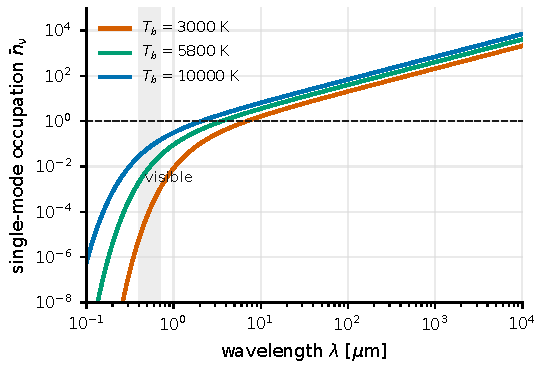
\includegraphics[width=0.82\linewidth]{figures/generated/chapter_03/ch03_blackbody_mode_occupation.pdf}
\caption{三条不同亮温黑体（3000、5800、10000\,K）的单模占有数 \(\bar n_\nu\) 随波长的变化，灰带标出可见光波段，虚线标出 \(\bar n_\nu=1\)。可见光灰带内，即便亮温是太阳量级，\(\bar n_\nu\) 也远小于 1（\(\sim10^{-2}\)），说明光学恒星光处在每模式弱光极限；向长波（红外、毫米波）一端，各温度曲线依次越过 \(\bar n_\nu=1\) 的虚线，进入 \(h\nu\ll k_{\rm B}T_b\) 的强占有数、近经典（Rayleigh--Jeans）极限。}
\label{fig:e05-mode-occupation}
\end{figure}

为什么这个"每模式很暗"如此要紧？因为它正是后面几章的出发点。既然每个相干时间窗里通常没有光子、偶尔才有一个，那么携带天体空间信息的，往往就是那一个被探测到的光子所在的模式——这直接引出弱热光（weak thermal light）的统计、光子成对到达的关联，以及超越衍射极限的量子超分辨（quantum super-resolution）思想。带着"太阳的每个模式其实很暗"这句话，我们就能进入下一阶段：看这些稀疏的光子在探测器上留下怎样的统计指纹。

\section{本章要点}
\label{sec:e05-summary}

\begin{itemize}
  \item \textbf{模式是光场的"广义纯音"。}把电磁场按一组正交模式（频率、空间形状、偏振、时间窗）展开，是傅里叶思想在电磁场上的推广，好处是每个模式彼此独立、可分别量子化。
  \item \textbf{每个模式就是一个谐振子。}这是全章枢纽：于是第 \ref{chap:e04} 章的量子化原样套上，得到每模式的 \(\hat a_k,\hat a_k^\dagger\)、对易关系 \([\hat a_i,\hat a_j^\dagger]=\delta_{ij}\) 和数算符 \(\hat n_k=\hat a_k^\dagger\hat a_k\)。
  \item \textbf{光子 = 某个模式的一次激发。}正频率场算符 \(\hat E^{(+)}=\sum_k\mathcal E_k u_k(\bm r)e^{-i\omega_k t}\hat a_k\) 里唯一的量子成分是 \(\hat a_k\)；探测一个光子就是在某模式里减少一个光子。\(\hat E^{(-)}\) 是它的厄米共轭。
  \item \textbf{Fock 态 \(|\{N_k\}\rangle\)} 把每个模式的光子数都钉死，是理解一切光态的坐标基。
  \item \textbf{一个观测通道往往是许多模式的和}：\(M\simeq(\Delta t/\tau_c)(A\Omega/\lambda^2)N_{\rm pol}\)，可见光下轻易达到成千上万。
  \item \textbf{光学恒星光处在每模式弱光极限}：\(\bar n_\nu=[\exp(h\nu/k_{\rm B}T_b)-1]^{-1}\)，太阳量级下 \(\bar n_\nu\approx7\times10^{-3}\)。总光子率高 \(\neq\) 每模式光子多。
\end{itemize}

\medskip
\noindent\textbf{想一想。}
\begin{enumerate}
  \item 若把滤光片带宽 \(\Delta\lambda\) 放宽 10 倍，相干时间 \(\tau_c\) 和一个 \(\Delta t\) 时间窗里的时间模式数各怎么变？
  \item 一根接收 seeing 糊开像的粗光纤，和一台衍射受限的成像仪，哪个的空间模式数 \(A\Omega/\lambda^2\) 更大？这对"看到的量子涨落深浅"意味着什么？
  \item 对同一颗恒星，为什么在 \(10\,\mu\mathrm{m}\) 中红外观测时，"每模式弱光"的图像会失效？用式 \eqref{eq:e05-occupation} 估一估此时的 \(\bar n_\nu\)。
\end{enumerate}


% ============================================================
\part{光的量子态与光子统计}
\chapter{单模光态：数态、相干态、热态、压缩态}
\label{chap:e06}

\begin{chapteropening}
上一章我们做成了一件大事：把整个电磁场拆成一堆模式，并证明\emph{每一个模式在数学上就是一个谐振子}——于是"光子"有了精确定义，它是某个模式的一次激发。可是同一个模式，就像同一个弹簧，可以处在千姿百态的量子态里。本章要回答的问题很朴素，也很关键：\textbf{在同一个模式里，光到底能装成哪几种样子？它们看起来有什么不同？}我们会发现，光子数是否钉死、相位是否稳定、强度是否涨落，会让四种典型光态——数态、相干态、热态、压缩态——即使平均光子数一模一样，也留下截然不同的"点击统计指纹"。为了把这四种光一次量到底，我们先造一把统一的尺子：\emph{零延迟成对因子} \(b_2\)。然后对每一种光，我们都手把手把它的 \(b_2\) 算出来——数态给 \(1-1/n\)（反聚束），相干态给 \(1\)（泊松基线），热态给 \(2\)（聚束）。这个"多出来的一倍"，正是后面强度干涉（Hanbury Brown--Twiss）赖以工作的种子。
\end{chapteropening}

\section{一把统一的尺子：零延迟成对因子}
\label{sec:e06-b2}

先想清楚我们到底要量什么。第 \ref{chap:e05} 章已经知道，望远镜每次"点击"背后站着一个湮灭算符 \(\hat a\)：某个模式里少了一个光子。如果我们盯住同一个模式，问"两个点击几乎同时到来的倾向有多强"，这就是光态最本质的区别之一——它不体现在平均有多亮，而体现在\emph{光子爱不爱扎堆}。

平均光子数谁都会算，就是数算符的期望 \(\langle\hat n\rangle\)。可只看平均，数态、相干态、热态可以完全一样（都调到 \(\langle\hat n\rangle=\bar n\)），却是三种截然不同的光。真正把它们分开的，是"成对"这件事：在同一个模式里，能凑出多少对光子？

\paragraph{为什么用阶乘矩，而不是平方}
\label{sec:e06-why-factorial}

一个初学者最自然的想法是用 \(\langle\hat n^2\rangle\) 来衡量"成对"。这恰恰是本节要纠正的第一个坑。设想模式里此刻有 \(N\) 个光子，我们要数"能从中挑出多少个\emph{有序光子对}"。挑第一个光子有 \(N\) 种选法，挑第二个——它必须是\emph{另一个}光子，不能是刚才那一个——只剩 \(N-1\) 种选法。所以有序对的数目是
\[
  N\times(N-1)=N(N-1),
\]
而不是 \(N\times N=N^2\)。两者相差的那一项 \(N^2-N(N-1)=N\)，正是"让同一个光子和它自己配对"的假项。物理上，\textbf{同一个光子不能和自己配成一对}：探测器吸收掉它一次，它就没了，不可能再被第二个探测器同时吸收。所以凡是涉及"两个点击"的量，正确的计数一定是 \(N(N-1)\)，即所谓的\emph{二阶阶乘矩}（second factorial moment）。这个"自配对要扣掉"的道理，会在第 \ref{chap:e07} 章讲光电探测的正规序（normal ordering）时再从算符层面证一遍；这里我们先从"数对子"的组合意义上把它认下来。

于是我们定义零延迟成对因子（zero-delay pair factor）：
\begin{equation}
  b_2\equiv\frac{\langle\hat n(\hat n-1)\rangle}{\langle\hat n\rangle^{2}} .
  \label{eq:e06-b2def}
\end{equation}
\begin{formulaexplain}
分子 \(\langle\hat n(\hat n-1)\rangle\) 是"平均能凑出多少对光子"（扣掉了自配对）；分母 \(\langle\hat n\rangle^2\) 是"若光子彼此独立、随机到达时应有的对数基线"。\(b_2\) 就是二者之比：光子扎堆的倾向相对随机基线放大了多少倍。
\end{formulaexplain}

逐个交代记号。\(\hat n=\hat a^\dagger\hat a\) 是数算符，本征值 \(N=0,1,2,\dots\) 是纯整数、无单位；\(\langle\cdot\rangle\) 是对光态求期望（纯态取内积，混合态取迹 \(\operatorname{Tr}(\rho\,\cdot)\)）。分子 \(\langle\hat n(\hat n-1)\rangle\) 无单位，是"平均对数"；分母 \(\langle\hat n\rangle^2\) 也无单位。所以 \(b_2\) 是一个纯数，它不关心这个模式有多亮（分母已经把亮度归一化掉了），只关心\emph{光子在同一模式里成对到来的倾向，相对于"各自独立、互不通气"的随机基线，是多还是少}。

为什么"独立随机"给出的基线恰好让分子约等于分母？下一节算相干态时会严格验证。这里先把三条判据摆出来，它是本章后面反复对照的标尺：
\begin{itemize}
  \item \(b_2=1\)：\textbf{独立泊松基线}。光子各来各的、互不通气，看到一个不改变马上再看到一个的概率。
  \item \(b_2>1\)：\textbf{聚束}（bunching）。光子爱扎堆，"要来一起来"，成对概率高于随机基线——热光就是如此。
  \item \(b_2<1\)：\textbf{反聚束}（antibunching），也叫\emph{亚泊松}。光子相互回避，"来了一个就不容易马上来第二个"，成对概率低于随机基线——这是纯量子效应，经典波做不到。
\end{itemize}

有了这把尺子，我们就逐一"量"四种光。策略始终一样：先写出该态的光子数分布 \(P(N)\)（或密度矩阵），算出 \(\langle\hat n\rangle\) 和 \(\langle\hat n(\hat n-1)\rangle\)，代进式 \eqref{eq:e06-b2def}。每一步都不跳。

\section{数态：光子数钉死的光}
\label{sec:e06-fock}

从最"干脆"的光开始。第 \ref{chap:e05} 章已经见过数态（number state）\(|n\rangle\)，又叫 Fock 态：它是数算符的本征态，\(\hat n|n\rangle=n|n\rangle\)，意思是这个模式里\emph{恰好}有 \(n\) 个光子，一个不多、一个不少、没有任何涨落。它的计数分布是一根孤零零的竖线：
\begin{equation}
  P(N)=\delta_{Nn}=
  \begin{cases}
    1, & N=n,\\
    0, & N\neq n.
  \end{cases}
  \label{eq:e06-fock-dist}
\end{equation}
\begin{formulaexplain}
\(P(N)\) 是"数到 \(N\) 个光子"的概率；\(\delta_{Nn}\) 是克罗内克符号（Kronecker delta），只有 \(N=n\) 时为 1、其余为 0。它说明数态测量光子数永远得到同一个值 \(n\)，毫无起伏。
\end{formulaexplain}

正因为 \(P(N)\) 只在 \(N=n\) 处非零，所有期望都退化成"直接代入 \(N=n\)"。平均光子数是
\[
  \langle\hat n\rangle=\sum_{N}N\,P(N)=n\cdot 1=n,
\]
二阶阶乘矩同样只留下 \(N=n\) 一项：
\[
  \langle\hat n(\hat n-1)\rangle=\sum_{N}N(N-1)\,P(N)=n(n-1).
\]
代进成对因子的定义 \eqref{eq:e06-b2def}：
\begin{equation}
  b_{2,\text{Fock}}=\frac{n(n-1)}{n^{2}}=\frac{n-1}{n}=1-\frac{1}{n}.
  \label{eq:e06-fock-b2}
\end{equation}
\begin{formulaexplain}
数态的成对因子只差随机基线 \(1\) 一个 \(1/n\)。光子数越少，反聚束越明显；\(n=1\) 时 \(b_2\) 一路压到 \(0\)。
\end{formulaexplain}

这条结果值得咀嚼。对任意有限 \(n\)，都有 \(b_2=1-1/n<1\)：数态总是\emph{反聚束}的。原因一目了然——模式里只有 \(n\) 个光子，用掉一个数对子就少一个"库存"，所以能凑的对数 \(n(n-1)\) 天然比"独立随机"的 \(n^2\) 少。特别地，取单光子态 \(n=1\)：
\[
  b_{2,\text{Fock}}(n=1)=1-\frac{1}{1}=0.
\]
这是反聚束的\emph{理想极限}。物理意义斩钉截铁：一个模式里只有一个光子，它被吸收一次就没了，绝不可能让两个探测器\emph{同时}各收到一个——所以"成对"概率精确为零。这正是单光子源（single-photon source）最珍贵的量子签名，实验室里的共振荧光可以清楚地做出 \(b_2\to 0\) \citep{1977PhRvL..39..691K}。

不过要提醒：天体光几乎从不以纯数态到达。源区里无数独立发射体、漫长的传播路径、望远镜和探测器都会把未观测的自由度混进来，把 \(b_2\) 从 \(0\) 一路拉回接近 \(1\)。数态在这里的价值，是给我们一个\emph{下限锚点}和一句提醒：点击统计测的是光子数的关联，而不是一条连续波形。当 \(n\to\infty\) 时 \(b_2\to 1\)，反聚束消失——光子一多，量子的"独占性"就淹没在数量里，这也预告了为什么明亮天体很难显出非经典统计。

\section{相干态：最像经典激光的光}
\label{sec:e06-coherent}

第 \ref{chap:e04} 章末尾预告过一种"最接近经典振动"的量子态；现在正式请它出场。相干态（coherent state）\(|\alpha\rangle\) 定义为湮灭算符的本征态：
\begin{equation}
  \hat a\,|\alpha\rangle=\alpha\,|\alpha\rangle,
  \qquad
  \bar n\equiv\langle\hat n\rangle=|\alpha|^{2}.
  \label{eq:e06-coherent-def}
\end{equation}
\begin{formulaexplain}
\(|\alpha\rangle\) 满足"被湮灭算符作用后自己不变、只乘一个复数 \(\alpha\)"。\(\alpha\) 是无量纲复振幅：它的模平方 \(|\alpha|^2\) 给平均光子数 \(\bar n\)，辐角 \(\arg\alpha\) 给相位。这是一支相位稳定、振幅确定的"经典波"的量子版本。
\end{formulaexplain}

先解释这个定义为什么"经典"。\(\alpha\) 是一个无量纲的复数，可以把它想成第 \ref{chap:e01} 章那支"旋转的箭头"（复振幅）：模长 \(|\alpha|\) 是振幅，辐角是相位，两者都确定，没有相位抖动——这正是理想激光的图像。稳定实验室激光在很多测量里都极接近相干态 \citep{1963PhRv..131.2766G}。而"\(\hat a|\alpha\rangle=\alpha|\alpha\rangle\)"这条奇特性质意味着：\emph{从相干态里拿走一个光子，它还是同一个相干态}——就像从一片浩瀚的相位一致的波里舀走一滴，波纹丝毫不改。这是它区别于数态的根本。

\paragraph{从定义推出泊松分布}
\label{sec:e06-coherent-poisson}

第 \ref{chap:e04} 章两次预告过"相干态的光子数服从泊松分布"，这里我们把它\emph{从定义推出来}，而不是空降。唯一的原料就是本征方程 \eqref{eq:e06-coherent-def}，加上第 \ref{chap:e05} 章的湮灭算符作用规则 \(\hat a|N\rangle=\sqrt{N}\,|N-1\rangle\)。

\textbf{第一步：把相干态写成数态的叠加。}数态 \(\{|N\rangle\}\) 是这个模式的完备基底，所以任何单模态都能展开成它们的线性组合。设
\[
  |\alpha\rangle=\sum_{N=0}^{\infty}c_N\,|N\rangle,
\]
其中待定系数 \(c_N=\langle N|\alpha\rangle\) 就是"这个态里含 \(N\) 光子成分"的振幅。把它代进本征方程左边，用 \(\hat a|N\rangle=\sqrt{N}\,|N-1\rangle\)（注意 \(N=0\) 项被湮灭掉、不贡献）：
\[
  \hat a\,|\alpha\rangle
  =\sum_{N=1}^{\infty}c_N\sqrt{N}\,|N-1\rangle
  =\sum_{M=0}^{\infty}c_{M+1}\sqrt{M+1}\,|M\rangle,
\]
最后一步令 \(M\equiv N-1\) 重新编号。而本征方程右边是
\[
  \alpha\,|\alpha\rangle=\sum_{M=0}^{\infty}\alpha\,c_M\,|M\rangle.
\]
\textbf{第二步：逐个数态比对系数，得到递推。}两边都是数态基底上的展开，对应系数必须相等，于是对每个 \(M\)：
\[
  c_{M+1}\sqrt{M+1}=\alpha\,c_M
  \quad\Longrightarrow\quad
  c_{M+1}=\frac{\alpha}{\sqrt{M+1}}\,c_M .
\]
\textbf{第三步：解递推。}从 \(c_0\) 出发逐级往上爬，每加一个光子就乘一个 \(\alpha/\sqrt{N}\)：
\[
  c_1=\frac{\alpha}{\sqrt1}c_0,\quad
  c_2=\frac{\alpha}{\sqrt2}c_1=\frac{\alpha^2}{\sqrt{2!}}c_0,\quad\dots\quad
  c_N=\frac{\alpha^{\,N}}{\sqrt{N!}}\,c_0 .
\]
\textbf{第四步：归一化定出 \(c_0\)。}要求 \(\langle\alpha|\alpha\rangle=\sum_N|c_N|^2=1\)。把上式代入，并点名使用指数级数 \(\sum_{N}x^N/N!=e^{x}\)（这里 \(x=|\alpha|^2\)）：
\[
  \sum_{N=0}^{\infty}|c_N|^2
  =|c_0|^2\sum_{N=0}^{\infty}\frac{|\alpha|^{2N}}{N!}
  =|c_0|^2\,e^{|\alpha|^2}=1
  \quad\Longrightarrow\quad
  |c_0|^2=e^{-|\alpha|^2}.
\]
取正实的 \(c_0=e^{-|\alpha|^2/2}\)（相位可任选，不影响概率）。至此相干态的数态展开就完全确定了。\textbf{第五步：读出光子数概率。}数到 \(N\) 个光子的概率正是该分量振幅的模平方：
\begin{equation}
  P(N)=\big|\langle N|\alpha\rangle\big|^2=|c_N|^2
  =\frac{|\alpha|^{2N}}{N!}\,e^{-|\alpha|^2}
  =e^{-\bar n}\,\frac{\bar n^{\,N}}{N!},
  \qquad N=0,1,2,\dots
  \label{eq:e06-poisson}
\end{equation}
\begin{formulaexplain}
\(P(N)\) 是数到 \(N\) 个光子的概率；\(\bar n=|\alpha|^2\) 是平均光子数；\(N!\) 是离散计数的归一化。它由本征方程一路推出，正是第 \ref{chap:e03} 章那条"独立随机到达"的泊松分布——相干态的光子彼此独立，各来各的。
\end{formulaexplain}

最后一步用了 \(\bar n=|\alpha|^2\)，把复振幅换成了平均光子数。式 \eqref{eq:e06-poisson} 就是\textbf{泊松分布}（Poisson distribution），它不是被断言的，而是从"\(\hat a|\alpha\rangle=\alpha|\alpha\rangle\)"一步步逼出来的：本征方程给递推，递推给系数，归一化定常数，模平方给概率。这里 \(\bar n=|\alpha|^2\) 无单位，\(N!\) 是 \(N\) 的阶乘。式 \eqref{eq:e06-poisson} 与第 \ref{chap:e03} 章讲散粒噪声时那条泊松分布\emph{完全同形}——这不是巧合：相干态的光子是彼此独立的随机事件，正是散粒噪声（shot noise）的来源，方差等于均值 \(\operatorname{Var}(N)=\bar n\)。

\paragraph{手把手算相干态的成对因子}
\label{sec:e06-coherent-b2}

现在用尺子量它。要算 \(b_2\)，我们需要二阶阶乘矩 \(\langle N(N-1)\rangle\)。把泊松分布 \eqref{eq:e06-poisson} 代进求和，一步不省：
\[
  \langle N(N-1)\rangle
  =\sum_{N=0}^{\infty}N(N-1)\,e^{-\bar n}\frac{\bar n^{\,N}}{N!}.
\]
\textbf{第一步：砍掉为零的项。}求和的每一项都带因子 \(N(N-1)\)。当 \(N=0\) 时 \(N(N-1)=0\)；当 \(N=1\) 时 \(N(N-1)=1\cdot 0=0\)。所以 \(N=0\) 和 \(N=1\) 两项对求和\emph{毫无贡献}，可以直接从 \(N=2\) 起加：
\[
  \langle N(N-1)\rangle
  =\sum_{N=2}^{\infty}N(N-1)\,e^{-\bar n}\frac{\bar n^{\,N}}{N!}.
\]
\textbf{第二步：约掉阶乘。}注意阶乘的定义 \(N!=N(N-1)(N-2)!\)，所以 \(N(N-1)/N!=1/(N-2)!\)。这一步把碍事的 \(N(N-1)\) 干净地消掉：
\[
  \langle N(N-1)\rangle
  =e^{-\bar n}\sum_{N=2}^{\infty}\frac{\bar n^{\,N}}{(N-2)!}.
\]
\textbf{第三步：换元求和。}令 \(m\equiv N-2\)（于是 \(N=2\) 对应 \(m=0\)，\(N\to\infty\) 对应 \(m\to\infty\)），并把 \(\bar n^{\,N}=\bar n^{\,2}\cdot\bar n^{\,m}\) 拆开，把与求和无关的 \(\bar n^2\) 提到外面：
\[
  \langle N(N-1)\rangle
  =e^{-\bar n}\,\bar n^{2}\sum_{m=0}^{\infty}\frac{\bar n^{\,m}}{m!}.
\]
\textbf{第四步：用指数级数。}最后那个求和正是指数函数的泰勒级数（Taylor series）\(\sum_{m=0}^{\infty}\bar n^{\,m}/m!=e^{\bar n}\)——这是一个我们点名使用的标准结果。于是 \(e^{-\bar n}\) 和 \(e^{\bar n}\) 恰好抵消：
\[
  \langle N(N-1)\rangle
  =e^{-\bar n}\,\bar n^{2}\,e^{\bar n}
  =\bar n^{2}.
\]
干净利落。既然 \(\langle N\rangle=\bar n\)，代进成对因子的定义 \eqref{eq:e06-b2def}：
\begin{equation}
  b_{2,\text{coh}}=\frac{\langle N(N-1)\rangle}{\langle N\rangle^{2}}
  =\frac{\bar n^{2}}{\bar n^{2}}=1.
  \label{eq:e06-coherent-b2}
\end{equation}
\begin{formulaexplain}
相干态的成对因子精确等于 \(1\)，与亮度 \(\bar n\) 无关。它就是我们标尺上的\emph{独立泊松基线}：光子各来各的，成对概率不多也不少。
\end{formulaexplain}

这个 \(b_2=1\) 就是式 \eqref{eq:e06-b2def} 里"独立随机基线"的严格来源。物理上它说的是一句很直白的话：\textbf{在相干态里看到一个光子，并不改变你马上再看到一个光子的条件概率}。光子之间不通气、不结伴、也不回避，纯粹独立。这也解释了为什么相干态既不聚束也不反聚束——它恰好卡在经典与量子的分界线上，是"最经典的量子态"。稳定激光近似如此；但要小心，\emph{天体的窄线或高亮温源并不自动是相干态}：独立发射区、湍流速度场、多重散射路径都会把相位抹平，结果反而更接近下一节的热态。

\section{热态：恒星连续谱的光}
\label{sec:e06-thermal}

轮到天文学家最常打交道的光了。恒星连续谱、行星际尘埃的散射光、绝大多数非相干源，其单模统计的出发点都是热态（thermal state）。它没有固定相位，是光子数基底上的\emph{混合态}，密度矩阵为
\begin{equation}
  \rho_{\text{th}}=\sum_{N=0}^{\infty}
  \frac{\bar n^{\,N}}{(1+\bar n)^{\,N+1}}\,|N\rangle\langle N|,
  \label{eq:e06-thermal-rho}
\end{equation}
\begin{formulaexplain}
\(\rho_{\text{th}}\) 是热态密度矩阵；它是各个数态 \(|N\rangle\) 的\emph{非相干}混合，权重按几何分布下降；\(\bar n\) 是这个模式的平均占有数。热态没有相位信息，只有"每个光子数出现的概率"。
\end{formulaexplain}

先读懂这条式子。\(|N\rangle\langle N|\) 是投影到"恰有 \(N\) 个光子"的算符，前面的系数就是数到 \(N\) 个光子的概率
\[
  P(N)=\frac{\bar n^{\,N}}{(1+\bar n)^{\,N+1}}
  =\frac{1}{1+\bar n}\left(\frac{\bar n}{1+\bar n}\right)^{N}.
\]
这是一个\textbf{几何分布}（geometric distribution），也就是第 \ref{chap:e05} 章推玻色占有数时遇到的玻色--爱因斯坦分布：概率随 \(N\) 单调下降，但拖着一条长长的高光子数尾巴。正是这条尾巴，让热光比相干光更爱"扎堆"。为验证归一化，用几何级数求和 \(\sum_{N=0}^\infty q^N=1/(1-q)\)（这里公比 \(q=\bar n/(1+\bar n)<1\)，收敛），得 \(\sum_N P(N)=\frac{1}{1+\bar n}\cdot\frac{1}{1-q}=\frac{1}{1+\bar n}\cdot(1+\bar n)=1\)，无误。

\paragraph{手把手算热态的成对因子}
\label{sec:e06-thermal-b2}

我们要两样东西：平均值 \(\langle N\rangle\) 和二阶阶乘矩 \(\langle N(N-1)\rangle\)。两者都从几何分布出发，用第 \ref{chap:e05} 章那套"对几何级数逐项求导"的现成技巧直接算出，一步不借外力；方差 \(\operatorname{Var}(N)\) 则作为它们的副产品顺手读出，用来讲聚束的物理。

\textbf{平均值。}这一步第 \ref{chap:e05} 章已经用"对几何级数逐项求导"的技巧算过，结论是
\[
  \langle N\rangle=\sum_{N=0}^{\infty}N\,P(N)=\bar n.
\]
也就是说，式 \eqref{eq:e06-thermal-rho} 里那个参数 \(\bar n\) 名副其实，正是平均光子数。

\textbf{二阶阶乘矩：从几何分布逐项求导，直接算出。}这是本节的核心量，我们不借任何未证的方差，而是把它从几何分布 \eqref{eq:e06-thermal-rho} 逐项算出来，方法和第 \ref{chap:e05} 章算均值时用的"对几何级数求导"完全同源。为了记号干净，记公比
\[
  q\equiv\frac{\bar n}{1+\bar n}\in(0,1),
  \qquad\text{于是}\quad 1-q=\frac{1}{1+\bar n},\quad P(N)=(1-q)\,q^{N}.
\]
一切从最基本的几何级数出发（公比 \(|q|<1\) 才收敛，这里满足）：
\[
  \sum_{N=0}^{\infty}q^{N}=\frac{1}{1-q}.
\]
把等号两边对 \(q\) 求导一次，就得到第 \ref{chap:e05} 章算均值时用过的那一式 \(\sum_N N q^{N-1}=1/(1-q)^2\)；我们这里\emph{再求一次导}，把 \(N(N-1)\) 从幂次里"敲"出来：
\[
  \frac{d^{2}}{dq^{2}}\sum_{N=0}^{\infty}q^{N}
  =\sum_{N=0}^{\infty}N(N-1)\,q^{\,N-2}
  =\frac{2}{(1-q)^{3}} .
\]
这一步点名使用一个标准结果：\emph{对收敛的幂级数，逐项求导与求和可以交换次序}（\(0<q<1\) 时该级数在 \(q\) 的一个邻域内一致收敛，故合法）。等号右边是把 \((1-q)^{-1}\) 求两次导得来的。两边乘上 \(q^{2}\)，把幂次补回 \(q^{N}\)：
\[
  \sum_{N=0}^{\infty}N(N-1)\,q^{N}=\frac{2q^{2}}{(1-q)^{3}} .
\]
现在给每一项配上前面的归一化因子 \((1-q)\)，就是我们要的期望：
\[
  \langle N(N-1)\rangle
  =(1-q)\sum_{N=0}^{\infty}N(N-1)\,q^{N}
  =(1-q)\cdot\frac{2q^{2}}{(1-q)^{3}}
  =\frac{2q^{2}}{(1-q)^{2}}
  =2\left(\frac{q}{1-q}\right)^{2}.
\]
最后把 \(q\) 换回 \(\bar n\)：由 \(q=\bar n/(1+\bar n)\) 与 \(1-q=1/(1+\bar n)\) 得 \(q/(1-q)=\bar n\)，于是
\begin{equation}
  \langle N(N-1)\rangle=2\bar n^{2}.
  \label{eq:e06-thermal-fm}
\end{equation}
\begin{formulaexplain}
热态的二阶阶乘矩是 \(2\bar n^2\)，恰好是相干态 \(\bar n^2\) 的\emph{两倍}。这多出来的一倍，就是后面 \(b_2=2\)（聚束）的全部来源，它由几何分布逐项求导硬算出来，没有借助任何未证事实。
\end{formulaexplain}

\textbf{顺手读出方差，把聚束讲清楚。}既然阶乘矩已经在手，方差就是它的直接副产品：用 \(\langle N^2\rangle=\langle N(N-1)\rangle+\langle N\rangle\)，得
\begin{equation}
  \operatorname{Var}(N)=\langle N^{2}\rangle-\langle N\rangle^{2}
  =\big[2\bar n^{2}+\bar n\big]-\bar n^{2}
  =\bar n+\bar n^{2}=\bar n(1+\bar n).
  \label{eq:e06-thermal-var}
\end{equation}
\begin{formulaexplain}
热态的方差比泊松的 \(\bar n\) 多出一项 \(\bar n^2\)。前一项 \(\bar n\) 是不可避免的散粒噪声（"光子是一颗颗的"），后一项 \(\bar n^2\) 是热光特有的\emph{强度涨落}——正是它带来聚束。
\end{formulaexplain}

把方差 \eqref{eq:e06-thermal-var} 拆成两块来读：\(\operatorname{Var}(N)=\underbrace{\bar n}_{\text{散粒噪声}}+\underbrace{\bar n^{2}}_{\text{强度涨落}}\)。第一项 \(\bar n\) 和相干态一样，是"光子离散"带来的、躲不掉的散粒噪声；第二项 \(\bar n^2\) 是热态\emph{额外多出来}的，来自光场强度本身在随机起伏——热光时亮时暗，亮的时候光子一起变多，暗的时候一起变少。这个"过量方差"是聚束的根源，请记住它。有了阶乘矩 \eqref{eq:e06-thermal-fm}，直接代进成对因子的定义 \eqref{eq:e06-b2def}：
\begin{equation}
  b_{2,\text{th}}=\frac{\langle N(N-1)\rangle}{\langle N\rangle^{2}}
  =\frac{2\bar n^{2}}{\bar n^{2}}=2.
  \label{eq:e06-thermal-b2}
\end{equation}
\begin{formulaexplain}
热态的成对因子精确等于 \(2\)，与亮度无关。它是随机基线的\emph{两倍}：热光的光子成对到来的概率，是独立随机情形的两倍。这就是聚束。
\end{formulaexplain}

这个 \(b_2=2\) 是本章的重头。那"多出来的一倍"（\(2\) 比基线 \(1\) 多出的 \(1\)）从哪来？它\emph{不是}探测器效应，也\emph{不是}什么新粒子作用，而是上面那第二项强度涨落 \(\bar n^2\) 的直接后果：热光在某一小段相干时间里强度偏高时，多个光子会\emph{一起}更容易到来；强度偏低时，它们又\emph{一起}变少。这种"要么一起多、要么一起少"的同进同退，就让光子倾向于成对、成群地到达——这就是聚束（bunching）的微观图像。

这一点的重要性怎么强调都不过分：\textbf{热光的 \(b_2=2\) 正是 Hanbury Brown--Twiss（强度干涉）赖以工作的种子}。1950 年代 Hanbury Brown 和 Twiss 正是靠测量两个探测器上光子到达的这种超量关联，第一次不靠振幅干涉就测出了恒星角直径 \citep{1956Natur.177...27B,1957RSPSA.242..300B}。没有热光那多出来的一倍，就没有可测的关联峰。第 \ref{chap:e08} 章我们会把这里的 \(b_2=2\) 精确地翻译成二阶相干函数 \(g^{(2)}(0)=2\)，第 \ref{chap:e10} 章再把它变成测角直径的工具。

一句必要的提醒：这里的 \(\bar n\) 是\emph{单模}平均占有数，不是望远镜每秒收到的总光子率。而且真实观测总是许多模式的和（第 \ref{chap:e05} 章的 \(M\)），多模平均会把这个"过量方差"稀释，使实测的聚束对比度小于单模理想的 \(2\)。这个稀释效应，也是第 \ref{chap:e08}、\ref{chap:e10} 章要反复处理的核心。

图 \ref{fig:e06-count-distributions} 把三种光在同一平均光子数下的计数分布画在一起，一眼就能看出差别的来源。

\begin{figure}[tbp]
\centering
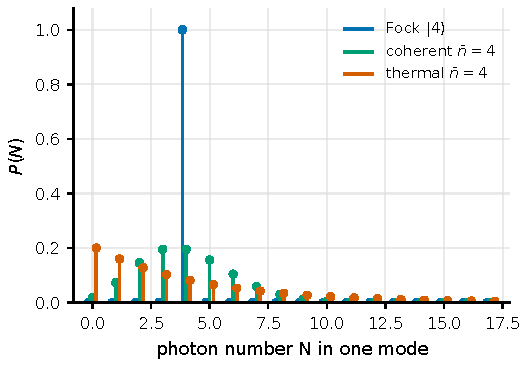
\includegraphics[width=0.82\linewidth]{figures/generated/chapter_03/ch03_state_count_distributions.pdf}
\caption{同一平均光子数附近，数态、相干态和热态给出完全不同的计数分布 \(P(N)\)。数态是一根钉死的竖线（光子数无涨落，\(b_2=1-1/n<1\)）；相干态是泊松分布，宽度约为 \(\sqrt{\bar n}\)（\(b_2=1\)）；热态是几何分布，拖着一条长长的高光子数尾巴（\(b_2=2\)，聚束）。正是这条尾巴，让热光在零延迟处更容易"成对"到达。}
\label{fig:e06-count-distributions}
\end{figure}

图 \ref{fig:e06-count-distributions} 的教益极简：\emph{平均光子数不是全部}。数态没有光子数涨落，相干态有泊松涨落，热态还额外背着一层强度涨落。天文强度干涉利用的，正是热态这最后一层涨落。

\section{压缩态：把量子噪声搬家}
\label{sec:e06-squeezed}

前三种光讲的是"光子数怎么分布"。压缩态（squeezed state）要讲一件不同的事：\emph{量子噪声可以在两个正交的场分量之间重新分配}。它不改变光子成对统计的那套语言，而是回到第 \ref{chap:e04} 章的正交分量（quadrature）图像。

先定义一个相位角 \(\theta\) 上的正交分量算符：
\begin{equation}
  \hat X_\theta=\frac{1}{2}\left(\hat a\,e^{-i\theta}+\hat a^{\dagger}e^{i\theta}\right).
  \label{eq:e06-quadrature}
\end{equation}
\begin{formulaexplain}
\(\hat X_\theta\) 是场沿相位方向 \(\theta\) 的"投影"，是第 \ref{chap:e04} 章位置/动量算符的推广：\(\theta=0\) 给类"位置"分量，\(\theta=\pi/2\) 给类"动量"分量。它无量纲，度量的是场在相空间某个方向上的坐标。
\end{formulaexplain}

逐个交代。\(\hat X_\theta\) 无量纲；\(\theta\) 是我们选定的相空间"观察角度"（弧度）；\(\hat a,\hat a^\dagger\) 是老熟人。取 \(\theta=0\) 得 \(\hat X_0=\tfrac12(\hat a+\hat a^\dagger)\)，正比于第 \ref{chap:e04} 章的位置算符 \(\hat x\)；取 \(\theta=\pi/2\) 得 \(\hat X_{\pi/2}=\tfrac{1}{2i}(\hat a-\hat a^\dagger)\)，正比于动量算符 \(\hat p\)。这两个正交方向就是相空间的"横轴与纵轴"。

关键的量子事实是：\textbf{真空态（以及任何相干态）在每一个方向上的涨落都相等}，方差都是 \(1/4\)。这个基线值不难算，值得当场兑现——它只用到真空的两条性质 \(\hat a|0\rangle=0\) 与对易关系 \([\hat a,\hat a^\dagger]=1\)。真空里 \(\langle\hat X_\theta\rangle=0\)（\(\hat a,\hat a^\dagger\) 的期望都为零），所以方差就等于 \(\langle\hat X_\theta^2\rangle\)。把定义 \eqref{eq:e06-quadrature} 平方展开：
\[
  \hat X_\theta^{2}
  =\frac14\big(\hat a\,e^{-i\theta}+\hat a^\dagger e^{i\theta}\big)^2
  =\frac14\big(\hat a^2 e^{-2i\theta}+\hat a^{\dagger 2}e^{2i\theta}
     +\hat a\hat a^\dagger+\hat a^\dagger\hat a\big).
\]
逐项对真空求期望：含 \(\hat a^2\) 的项因 \(\hat a|0\rangle=0\) 归零；含 \(\hat a^{\dagger2}\) 的项其厄米共轭同样归零；\(\hat a^\dagger\hat a\,|0\rangle=0\)（数算符作用在真空上为零）；只剩 \(\langle 0|\hat a\hat a^\dagger|0\rangle\)，用 \(\hat a\hat a^\dagger=\hat a^\dagger\hat a+[\hat a,\hat a^\dagger]=\hat n+1\) 得 \(\langle0|\hat a\hat a^\dagger|0\rangle=0+1=1\)。于是
\[
  \Delta X_\theta^{2}\big|_{\text{真空}}=\langle\hat X_\theta^2\rangle
  =\frac14\cdot 1=\frac{1}{4}\qquad(\text{对一切 }\theta).
\]
结果和 \(\theta\) 无关，正说明真空在相空间里是一个各向同性的"圆斑"——这也是下一节相空间图像的出发点。海森堡不确定性要求两个正交方向方差之积不小于 \(\tfrac{1}{16}\)，真空恰好取到这个最小值（\(\tfrac14\times\tfrac14=\tfrac1{16}\)）。

压缩态做的事，是把这个圆斑\emph{捏扁}：沿某个方向把方差压到 \(1/4\) 以下，代价是共轭方向的方差被相应抬高。设压缩参数（squeezing parameter）为 \(r\ge0\)，则
\begin{equation}
  \Delta X_{\text{sq}}^{2}=\frac{1}{4}\,e^{-2r},
  \qquad
  \Delta X_{\text{anti}}^{2}=\frac{1}{4}\,e^{+2r}.
  \label{eq:e06-squeeze-var}
\end{equation}
\begin{formulaexplain}
被压缩方向的方差乘上 \(e^{-2r}<1\)（噪声变小），被反压缩方向的方差乘上 \(e^{+2r}>1\)（噪声变大）。\(r\) 越大，一个方向越"扁"、另一个方向越"胖"。
\end{formulaexplain}

这个 \(e^{\mp 2r}\) 的形状来自单模压缩变换：它把相空间沿一个正交方向的振幅尺度乘上 \(e^{-r}\)，方差（尺度的平方）就乘上 \(e^{-2r}\)；共轭方向的尺度乘 \(e^{+r}\)，方差乘 \(e^{+2r}\)。最要紧的是把两个方差乘起来：
\[
  \Delta X_{\text{sq}}^{2}\cdot\Delta X_{\text{anti}}^{2}
  =\frac14 e^{-2r}\cdot\frac14 e^{+2r}
  =\frac{1}{16}\,e^{-2r+2r}
  =\frac{1}{16}.
\]
乘积\emph{仍然}是 \(1/16\)，和真空一模一样！这句话是理解压缩的钥匙：\textbf{压缩没有消灭量子噪声，它只是把噪声从一个方向搬到了另一个方向}——按下葫芦起了瓢，总量守恒。你可以让某个正交分量安静到真空以下，但必须让它的共轭分量吵闹起来做补偿。

实验文献常用分贝（dB）记噪声相对真空的比例：\(10\log_{10}(e^{-2r})\)。例如噪声方差降到真空的十分之一，就是 \(-10\,\text{dB}\)。现代压缩光实验在 \(1064\,\text{nm}\) 附近已能稳定做出 \(10\)–\(15\,\text{dB}\) 的噪声压低，并已用在引力波探测器上把散粒噪声压到标准量子极限以下 \citep{1983Natur.306..141W,2016PhRvL.117k0801V}。

但对天文学要泼一盆冷水：\textbf{普通恒星连续谱并不默认具有压缩}。热态和相干态在每个正交方向上的涨落都不小于真空，谈不上"压扁"。压缩是一种需要非线性光学过程（如参量下转换）精心制备的非经典态，恒星、星云这类自然热源不会自发产生它。我们介绍压缩态，一是为了补全"同一个模式能装哪几种光"的完整图谱，二是因为它在\emph{仪器端}至关重要——未来量子增强的望远镜后端可能用压缩光来突破散粒噪声。但把它当成天体光的默认模型，是一个要避免的误区。

\section{弱热光极限：为超分辨埋下的线}
\label{sec:e06-weak}

最后一节把热态推到天文最常见的角落：\emph{每个模式其实很暗}。第 \ref{chap:e05} 章算过，可见光下恒星的单模占有数 \(\bar n_\nu\sim10^{-2}\ll1\)。在这个弱热光（weak thermal light）极限下，热态会退化成一个特别简单、特别有用的形式。

从几何分布出发，把 \(P(N)\) 在 \(\bar n\ll 1\) 时展开到最低阶。零光子的概率是
\[
  P(0)=\frac{1}{1+\bar n}\simeq 1-\bar n+\mathcal O(\bar n^{2}),
\]
这里用了 \((1+\bar n)^{-1}=1-\bar n+\bar n^2-\cdots\) 的几何级数展开（\(\bar n<1\) 收敛），只保留到一阶。一光子的概率是
\[
  P(1)=\frac{\bar n}{(1+\bar n)^{2}}
  \simeq\bar n\,(1-2\bar n+\cdots)
  \simeq\bar n+\mathcal O(\bar n^{2}).
\]
两光子及以上的概率则是
\[
  P(N\ge 2)=\mathcal O(\bar n^{2}),
\]
因为 \(P(2)=\bar n^2/(1+\bar n)^3\sim\bar n^2\)，是更高阶的小量。也就是说，弱热光里\emph{绝大多数相干时间窗是空的}，偶尔有一个窗里蹦出一个光子，而两个光子同窗则是二阶稀有事件。

把这个层级写成密度矩阵，就得到弱热光的标准记账形式：
\begin{equation}
  \rho\simeq(1-\varepsilon)\,\rho_0+\varepsilon\,\rho_1+\mathcal O(\varepsilon^{2}),
  \qquad
  \varepsilon\equiv\bar n\ll 1,
  \label{eq:e06-weak}
\end{equation}
\begin{formulaexplain}
\(\rho_0=|0\rangle\langle 0|\) 是真空部分（占比 \(1-\varepsilon\)），\(\rho_1=|1\rangle\langle 1|\) 是一光子部分（占比 \(\varepsilon\)），\(\varepsilon=\bar n\) 是单模平均光子数。弱热光就是"大多为空、偶尔一个"的稀疏光子流。
\end{formulaexplain}

逐个交代：\(\rho_0\) 是真空态的密度矩阵，\(\rho_1\) 是单光子态的密度矩阵，小参数 \(\varepsilon=\bar n\) 无量纲，恰好等于上面 \(P(1)\) 的最低阶——所以\emph{把 \(\varepsilon\) 认成"该模式在该时间窗里的平均光子数"是精确的}。式 \eqref{eq:e06-weak} 说的是：光态几乎全是真空，只掺进了一点点单光子成分。这个"一点点"，正是携带天体信息的东西。

为什么要为它专门开一节？因为它是后面\textbf{量子超分辨}（quantum super-resolution）的出发点。既然每个相干时间窗里通常没有光子、偶尔才有一个，那么真正携带天体空间信息的，就是那被探测到的\emph{一光子模式}的空间结构。Tsang、Nair 与 Lu 的弱热光超分辨理论正是从式 \eqref{eq:e06-weak} 这样的展开出发，证明只要能巧妙地测量这一个光子的模式（而不是简单地数强度），就能突破经典的瑞利极限 \citep{2015Optic...2..646T,2016PhRvX...6c1033T}。我们会在第 \ref{chap:e12} 章把这条线接上，讲 SPADE（spatial-mode demultiplexing）如何逼近两颗靠得极近的星的分辨极限。这也和天文事件表天然吻合：零光子的时间窗根本不会被存进文件，留在数据里的，就是那些带时间戳的、稀疏的单光子点击。

\section{相空间图像：把四种光画成一张图}
\label{sec:e06-phasespace}

把这一章收束到一张\emph{看得见}的图上。相空间（phase space）用两个正交分量 \(X\)（横轴）和 \(P\)（纵轴）张成一个平面，把一个模式的量子态画成这个平面上的一团"概率云"——云的中心是平均场，云的胖瘦是涨落。上一节说过，真空和相干态在每个方向的涨落都是 \(1/4\)，所以画出来是一个各向同性的\emph{圆斑}。四种光在这张图上各有各的样子：

\begin{itemize}
  \item \textbf{真空态}：圆斑在原点，半径由 \(1/4\) 的涨落定出。这是所有噪声的"底座"。
  \item \textbf{相干态}：一个\emph{一模一样大小的圆斑}，只是被平移到离原点 \(|\alpha|\) 处。它把真空的圆斑整体搬了个家，形状不变——所以相干态是"移动了的真空"，噪声和真空一样小、一样各向同性。这对应它的 \(b_2=1\)。
  \item \textbf{热态}：一个\emph{中心仍在原点、但更胖的圆}。它没有固定相位（辐角完全随机），又有强度涨落，所以概率云向四面八方摊开，半径随 \(\bar n\) 增大。这个"更胖"，正是热态额外方差 \(\bar n^2\) 的相空间形象，也对应它的 \(b_2=2\)。
  \item \textbf{压缩态}：一个\emph{被压扁的椭圆}。沿被压缩方向窄到真空以下（\(\tfrac14 e^{-2r}\)），沿共轭方向被撑胖（\(\tfrac14 e^{+2r}\)），但椭圆的面积（两个半轴之积对应的方差乘积 \(1/16\)）和圆斑一样——"噪声搬家、面积守恒"在图上就是"圆压成等面积的椭圆"。
\end{itemize}

图 \ref{fig:e06-phase-space} 把相干态、热态、压缩态的这三种"云"并排画了出来。

\begin{figure}[tbp]
\centering
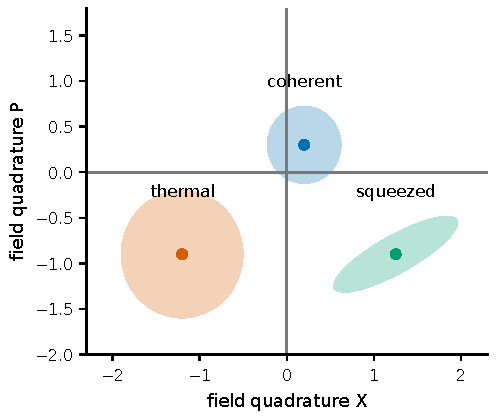
\includegraphics[width=0.72\linewidth]{figures/generated/chapter_03/ch03_phase_space_states.pdf}
\caption{相空间中三类单模光态的涨落形状。相干态是与真空同样大小、只是被平移的圆斑（"移动的真空"）；热态因随机相位和强度涨落而摊成更胖的圆；压缩态把一个正交方向的涨落压到真空以下、同时把共轭方向抬高，成为等面积的椭圆。记住：区分不同光态的，首先是涨落与关联的\emph{形状}，而不只是平均强度。}
\label{fig:e06-phase-space}
\end{figure}

这张相空间图给出一句能带走的话：\emph{不同光态的区别，首先表现为涨落和关联的形状，而不只是平均强度}。同样的亮度，可以是一个安分的圆斑（相干态）、一个躁动的胖圆（热态），或一个被捏扁的椭圆（压缩态）——而正是这些形状，决定了探测器上点击的成对统计。带着这幅图，我们就能进入第 \ref{chap:e07} 章，看这些光态如何在光电探测器上真正变成一串可分析的事件。

\section{本章要点}
\label{sec:e06-summary}

\begin{itemize}
  \item \textbf{尺子：零延迟成对因子} \(b_2=\langle\hat n(\hat n-1)\rangle/\langle\hat n\rangle^2\)。分子用阶乘矩 \(\hat n(\hat n-1)\) 而非 \(\hat n^2\)，因为"同一个光子不能和自己配对"，自配对要扣掉。\(b_2=1\) 是独立泊松基线，\(>1\) 聚束，\(<1\) 反聚束（非经典）。
  \item \textbf{数态 \(|n\rangle\)}：\(P(N)=\delta_{Nn}\)，光子数钉死。\(\langle\hat n\rangle=n\)、\(\langle\hat n(\hat n-1)\rangle=n(n-1)\)，给 \(b_2=1-1/n<1\)。单光子 \(n=1\) 给 \(b_2=0\)，是反聚束的理想极限。
  \item \textbf{相干态 \(|\alpha\rangle\)}：\(\hat a|\alpha\rangle=\alpha|\alpha\rangle\)，\(\bar n=|\alpha|^2\)，计数是泊松分布。逐项求和（砍零项、约阶乘、换元、用指数级数）得 \(\langle N(N-1)\rangle=\bar n^2\)，故 \(b_2=1\)。看到一个光子不改变马上再看到一个的概率。
  \item \textbf{热态 \(\rho_{\text{th}}\)}：几何/玻色分布，\(\langle N\rangle=\bar n\)、\(\operatorname{Var}=\bar n(1+\bar n)\)、\(\langle N(N-1)\rangle=2\bar n^2\)，故 \(b_2=2\)。多出的一倍来自强度涨落（亮时一起多、暗时一起少），这正是 Hanbury Brown--Twiss 聚束的种子。
  \item \textbf{压缩态}：正交分量 \(\hat X_\theta=\tfrac12(\hat a e^{-i\theta}+\hat a^\dagger e^{i\theta})\)，真空方差 \(1/4\)；压缩/反压缩方差 \(\tfrac14 e^{\mp 2r}\)，乘积仍 \(1/16\)——噪声被搬家、不被消灭。普通恒星光不默认压缩，它主要在仪器端有用。
  \item \textbf{弱热光极限}：\(\bar n\ll1\) 时 \(\rho\approx(1-\varepsilon)\rho_0+\varepsilon\rho_1\)，\(\varepsilon=\bar n\)，由几何分布最低阶 \(P(0)\approx1-\bar n\)、\(P(1)\approx\bar n\) 得到。大多数时间窗为空，携带空间信息的是那个被探测到的单光子模式——通往第 \ref{chap:e12} 章超分辨。
  \item \textbf{相空间}：相干态=移动的真空圆斑，热态=更胖的圆，压缩态=等面积的扁椭圆。区分光态的首先是涨落形状，而非平均强度。
\end{itemize}

\medskip
\noindent\textbf{想一想。}
\begin{enumerate}
  \item 把两个独立的单模热光（各自 \(b_2=2\)）非相干地叠加成一个"双模"通道，观测到的成对因子会大于 2、等于 2 还是小于 2？这和第 \ref{chap:e05} 章"多模稀释"的说法一致吗？
  \item 对同一个平均光子数 \(\bar n=10\)，数态、相干态、热态的计数方差各是多少？哪个最"安静"、哪个最"吵"？
  \item 若某个天体源被测得 \(b_2<1\)，能立刻断言它是非经典光源吗？在下结论前，你还需要排除哪些会把 \(b_2\) 拉高或拉低的仪器与混合效应（回顾第 \ref{chap:e05} 章的模式数 \(M\)）？
\end{enumerate}

\chapter{光电探测与光子计数：为什么数的是 n(n-1)}
\label{chap:e07}

\begin{chapteropening}
到上一章为止，我们已经把光"读"得很透了：光是一组模式的激发，每个模式就是一个谐振子，光子是模式里的一份能量，而数态、相干态、热态这三种光即使亮度相同，光子成对到达的倾向 \(b_2\) 却截然不同（第 \ref{chap:e06} 章）。可这一切都还停在"光态"这一侧。望远镜那一侧交回来的，从来不是一个波函数，而是一串冷冰冰的点击——某时刻，某像素，咔哒一声。本章要架的，正是这两侧之间的桥：光态究竟怎样变成探测器上的一串计数？我们会一步步弄清三件事。第一，为什么"探测一个光子"这件事，在数学上逼着我们去数 \(n(n-1)\) 而不是 \(n^2\)——那个被减掉的 \(n\)，正是"同一个光子不能和自己配对"。第二，怎样把一张事件表切成一格格时间门，用一个叫 Mandel \(Q\) 的数，一眼看出这束光比泊松更"抱团"还是更"规矩"。第三，为什么教科书上气势磅礴的 \(g^{(2)}(0)=2\)，到了真实望远镜上会缩水成 \(1+10^{-3}\) 甚至 \(1+10^{-6}\) 这样的小数——不是信号没了，而是被成千上万个模式稀释了。走完这一章，你手里就有了把"光的量子态"翻译成"可以真正拿去拟合的计数统计量"的全套换算。
\end{chapteropening}

\section{点击从哪来：探测就是吸收一个光子}
\label{sec:e07-absorption}

先回到最朴素的问题：探测器"看见"一个光子，物理上到底发生了什么？

不是光子撞上一面墙被弹回来，也不是它像小球一样被"接住"。真实的光电探测（photodetection）是一次\emph{吸收}：光场里一份能量被交给探测器（打出一个光电子、触发一次雪崩、翻转一个像素），与此同时，\textbf{光场里少了一个光子}。第 \ref{chap:e05} 章我们已经反复强调过这句话，并把它写成算符语言：吸收只用得上正频率场算符 \(\hat E^{(+)}\)，因为 \(\hat E^{(+)}\) 里装的是湮灭算符 \(\hat a\)（拿走一个光子），而不是产生算符 \(\hat a^\dagger\)。

现在只盯住一个模式。此时正频率场正比于该模式的湮灭算符，\(\hat E^{(+)}\propto\hat a\)。量子探测理论（Glauber）告诉我们一条干净的规则：\textbf{探测器在某一瞬间"咔哒"一声的概率，正比于把湮灭算符夹在光态里取平均。}一次点击对应一次吸收，所以单次点击率正比于

\begin{equation}
  p_1\ \propto\ \big\langle\,\hat E^{(-)}\hat E^{(+)}\,\big\rangle
  \ \propto\ \big\langle\,\hat a^\dagger\hat a\,\big\rangle
  =\langle\hat n\rangle .
  \label{eq:e07-single-click}
\end{equation}
\begin{formulaexplain}
单次点击概率正比于 \(\langle\hat a^\dagger\hat a\rangle=\langle\hat n\rangle\)。\(\hat a\) 先作用（吸收那一个光子），\(\hat a^\dagger\) 是它的厄米共轭；夹在一起取平均就是"平均有几个光子"。一句话：\emph{点击率跟着光子数走}。
\end{formulaexplain}

逐个符号交代。\(\hat E^{(+)}\)、\(\hat E^{(-)}=[\hat E^{(+)}]^\dagger\) 是正、负频率场算符（第 \ref{chap:e05} 章）；单模下它们分别正比于 \(\hat a\) 与 \(\hat a^\dagger\)，都无量纲（比例常数吸收进探测效率里）。\(\hat n=\hat a^\dagger\hat a\) 是光子数算符，本征值 \(N=0,1,2,\dots\)，纯整数无单位。尖括号 \(\langle\cdot\rangle\) 是对光态求量子期望。式 \eqref{eq:e07-single-click} 的物理含义再直白不过：想让探测器多响，就得让模式里平均光子多。这也是为什么在第 \ref{chap:e05} 章里，"每个模式其实很暗"（\(\bar n_\nu\sim10^{-2}\)）会直接翻译成"单个模式的点击率其实很低"。

\paragraph{两次符合点击：正规序自动扣掉"自己和自己配对"}
\label{sec:e07-normal-ordering}

真正有意思的是两次点击。设想我们问的不再是"响一声的概率"，而是"在（几乎）同一时刻响\emph{两}声的概率"——这正是 Hanbury Brown--Twiss 强度干涉、符合计数、二阶相干测量的核心量。两次点击意味着两次吸收：光场里\emph{接连}少了两个光子。按同样的探测规则，把两个 \(\hat E^{(+)}\) 排在一起，两次符合点击率正比于

\begin{equation}
  p_2\ \propto\ \big\langle\,\hat E^{(-)}\hat E^{(-)}\hat E^{(+)}\hat E^{(+)}\,\big\rangle
  \ \propto\ \big\langle\,\hat a^\dagger\hat a^\dagger\hat a\,\hat a\,\big\rangle .
  \label{eq:e07-two-click}
\end{equation}
\begin{formulaexplain}
两次符合点击概率正比于 \(\langle\hat a^\dagger\hat a^\dagger\hat a\hat a\rangle\)：所有湮灭算符（吸收）排在右边、所有产生算符排在左边。这种"产生在左、湮灭在右"的排法叫\textbf{正规序}（normal ordering），它正是"两次点击对应两次真实吸收"的数学写照。
\end{formulaexplain}

注意 \eqref{eq:e07-two-click} 里算符的次序：两个 \(\hat a\)（吸收）挨着排在最右，两个 \(\hat a^\dagger\) 排在最左。这个"湮灭全在右、产生全在左"的排列就叫正规序。它不是人为约定，而是探测的物理强加的：探测器只会对\emph{真实被吸收}的光子响应，所以每一次点击对应一个 \(\hat a\) 作用在态上，两次点击就把两个 \(\hat a\) 先后作用上去。

现在到了本章标题里那个问题的关键。式 \eqref{eq:e07-two-click} 里的算符组合 \(\hat a^\dagger\hat a^\dagger\hat a\hat a\) 到底等于什么？我们不猜，直接用第 \ref{chap:e05} 章反复用过的\emph{唯一}一条代数事实——对易关系 \([\hat a,\hat a^\dagger]=1\)，也就是 \(\hat a\hat a^\dagger=\hat a^\dagger\hat a+1\)——把它一步步化开。目标是把它写成数算符 \(\hat n=\hat a^\dagger\hat a\) 的函数。

先看数算符的平方：
\[
  \hat n^2=(\hat a^\dagger\hat a)(\hat a^\dagger\hat a)
  =\hat a^\dagger\,\underbrace{(\hat a\,\hat a^\dagger)}_{=\,\hat a^\dagger\hat a+1}\,\hat a
  =\hat a^\dagger(\hat a^\dagger\hat a+1)\hat a
  =\hat a^\dagger\hat a^\dagger\hat a\,\hat a+\hat a^\dagger\hat a .
\]
中间那一步就是把 \(\hat a\hat a^\dagger\) 换成 \(\hat a^\dagger\hat a+1\)，这是全推导用到的唯一非平凡代数。把右边第二项认出来是 \(\hat n\)，整理即得正规序与数算符的桥梁：
\begin{equation}
  \hat a^\dagger\hat a^\dagger\hat a\,\hat a
  =\hat n^2-\hat n
  =\hat n(\hat n-1).
  \label{eq:e07-normal-identity}
\end{equation}
\begin{formulaexplain}
正规序的双光子算符\emph{精确}等于 \(\hat n(\hat n-1)\)。若模式里有 \(N\) 个光子，可组的"有序光子对"是 \(N^2\)，但其中 \(N\) 个是"同一个光子与自己配对"；正规序自动把这 \(N\) 个假对减掉，剩下 \(N(N-1)\) 个\emph{真}对。
\end{formulaexplain}

这行式子值得停下来品味。它说的是：\textbf{正规序 = 自动扣掉自配对。}想象某个瞬间模式里恰有 \(N\) 个光子。若不动脑子，把"第一次数到的光子"和"第二次数到的光子"随意搭配，一共有 \(N\times N=N^2\) 种\emph{有序}选法。可其中有 \(N\) 种是"第一次和第二次数到的是\emph{同一个}光子"——这在物理上不可能，因为一次符合探测需要一个 START 脉冲和一个 STOP 脉冲，它们必须来自\emph{两次不同的吸收}，同一个光子被吸收后就没了，绝不会再触发第二声。于是真正可用的有序光子对数是 \(N(N-1)=N^2-N\)，那减掉的 \(N\) 正是自配对。式 \eqref{eq:e07-normal-identity} 里 \(\hat n^2\) 与 \(\hat n(\hat n-1)\) 差的那一项 \(\hat n\)，一个符号不多一个符号不少，就是这些自配对。

这也正是第 \ref{chap:e06} 章那个成对因子 \(b_2\) 的来历。回忆一下，我们在那里把单模零延迟成对倾向定义为
\[
  b_2\equiv\frac{\langle\hat n(\hat n-1)\rangle}{\langle\hat n\rangle^2},
\]
并算出数态给 \(b_2=1-1/n\)（反聚束）、相干态给 \(b_2=1\)（泊松基线）、热态给 \(b_2=2\)（聚束）。现在我们终于明白：分子上那个 \(\langle\hat n(\hat n-1)\rangle\) 不是谁拍脑袋定义的怪东西，而是探测器\emph{物理上只能数真对}的必然结果。把 \eqref{eq:e07-single-click} 与 \eqref{eq:e07-two-click} 归一化，就得到

\begin{equation}
  \frac{p_2}{p_1^2}\ \propto\
  \frac{\langle\hat a^\dagger\hat a^\dagger\hat a\hat a\rangle}{\langle\hat a^\dagger\hat a\rangle^2}
  =\frac{\langle\hat n(\hat n-1)\rangle}{\langle\hat n\rangle^2}
  =b_2 .
  \label{eq:e07-b2-from-clicks}
\end{equation}
\begin{formulaexplain}
把"两声一起响"的概率除以"两次独立响一声"的概率，就得到成对因子 \(b_2\)。它是探测器实测的量：\(b_2>1\) 光子爱抱团（聚束），\(b_2<1\) 光子相互回避（反聚束），\(b_2=1\) 各来各的（泊松）。
\end{formulaexplain}

一句话收束这一节：\textbf{探测器数的永远是"不同吸收事件"之间的关联，也就是 \(\langle n(n-1)\rangle\)，而不是一条连续波形，也不是 \(\langle n^2\rangle\)。}正规序不是形式主义的花招，它就是"一个光子只能被吸收一次"这条最硬的物理事实。图 \ref{fig:e07-factorial-moments} 把这件事画了出来：同一个计数分布，用 \(N^2\) 加权和用 \(N(N-1)\) 加权，权重差的就是那条自配对的对角线。

\begin{figure}[tbp]
\centering
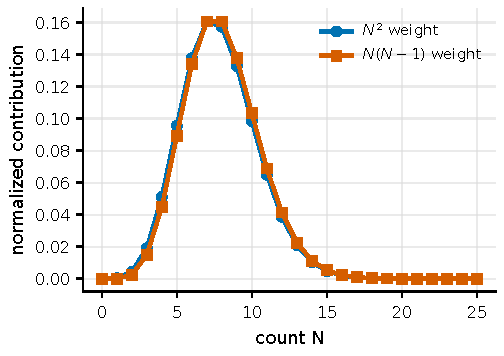
\includegraphics[width=0.86\linewidth]{figures/generated/chapter_04/ch04_factorial_moments.pdf}
\caption{普通二阶矩 \(N^2\) 与阶乘矩（factorial moment）\(N(N-1)\) 对不同光子数 \(N\) 的加权不同。符合探测只关心由\emph{不同}光子组成的有序对，因此正规序自动把 \(N^2-N(N-1)=N\) 这一项"同一光子与自己配对"的假贡献扣掉。这正是为什么二阶光子统计里出现的是 \(\langle N(N-1)\rangle\)，而不是 \(\langle N^2\rangle\)。}
\label{fig:e07-factorial-moments}
\end{figure}

\section{把事件表切成时间门：均值、方差与 Mandel 参数}
\label{sec:e07-time-gate}

上一节讲的是"瞬时"的算符期望。可真实望远镜交回来的是一张带时间戳的事件表——一长串"某个光子在某时刻到达"的记录（这张表的结构、时钟、死时间等硬件细节，留到第 \ref{chap:e13} 章细讲）。要把 \eqref{eq:e07-b2-from-clicks} 那样的算符期望，变成能真正从数据里算出来的数，我们需要一个具体的操作：\textbf{把连续时间切成一格一格宽度为 \(\Delta t\) 的"时间门"（time gate/bin），数每一格里落进了几个光子。}

设第 \(k\) 格时间门里的计数为 \(N_k\)（无量纲整数）。把许多格的计数收集起来，就得到一个计数分布 \(P(N)\)：出现 \(N\) 个光子的时间门占多大比例。对这个分布，我们关心两个最基本的统计量——均值和方差：

\begin{equation}
  \bar N=\langle N\rangle=\sum_{N=0}^{\infty}N\,P(N),
  \qquad
  \sigma_N^2=\big\langle N^2\big\rangle-\bar N^{\,2}
  =\sum_{N=0}^{\infty}(N-\bar N)^2\,P(N).
  \label{eq:e07-mean-var}
\end{equation}
\begin{formulaexplain}
\(\bar N\) 是每个时间门的\emph{平均}计数，\(\sigma_N^2\) 是计数在各门之间\emph{起伏}的大小（方差）。均值告诉你"平均多亮"，方差告诉你"忽明忽暗到什么程度"。判断光的量子性，看的是后者相对前者的大小。
\end{formulaexplain}

逐个交代：\(\bar N\) 无量纲，是门宽 \(\Delta t\) 内的平均光子数，等于计数率 \(r\)（单位 \(\mathrm{s^{-1}}\)）乘门宽，\(\bar N=r\,\Delta t\)。\(\sigma_N^2\) 也无量纲，是计数偏离均值的平方的平均。这里必须记住一件在天文里很反直觉的事：门宽 \(\Delta t\) 通常选得很小，比如 \(\Delta t=1\,\mathrm{ns}\)，而可见光点源的计数率也许只有 \(r=10^6\,\mathrm{s^{-1}}\)，于是

\[
  \bar N=r\,\Delta t=(10^6\,\mathrm{s^{-1}})(10^{-9}\,\mathrm{s})=10^{-3}.
\]

也就是说，\emph{一千个时间门里才有大约一个装着光子}，绝大多数门是空的（\(N=0\)），偶尔一个门里有 \(N=1\)，同一个门里有两个光子的机会小到 \(\sim10^{-6}\)。强度相关信号从来不是从一条肉眼可见的"光变曲线起伏"里读出来的，而是从 \(10^8\)、\(10^{12}\) 个时间门的微小统计偏差里，一点点累加出来的。这也是为什么我们必须用统计量、而不是用眼睛，来判断光的性质。

\paragraph{以泊松为零点：Mandel Q}
\label{sec:e07-mandel-q}

现在需要一把尺子，来量"这束光比随机到达更抱团、还是更规矩"。天然的零点是\textbf{泊松分布}（Poisson distribution）：若光子各来各的、彼此独立（相干态就是这样，见第 \ref{chap:e06} 章），计数服从泊松统计，它有一个招牌性质——\emph{方差恰好等于均值}：
\[
  \text{泊松：}\quad \sigma_N^2=\bar N .
\]
（这条我们在第 \ref{chap:e06} 章由 \(P(N)=e^{-\bar N}\bar N^N/N!\) 直接算过，是散粒噪声 shot noise 的定义。）把这条当零点，Mandel 用一个无量纲的数——\textbf{Mandel 参数}（Mandel \(Q\) parameter）——来度量偏离：

\begin{equation}
  Q\equiv\frac{\sigma_N^2-\bar N}{\bar N}.
  \label{eq:e07-mandel-q}
\end{equation}
\begin{formulaexplain}
\(Q\) 把泊松的 \(\sigma_N^2=\bar N\) 定为零点，量的是"方差比均值多出（或少掉）几成"。\(Q=0\) 泊松（相干态），\(Q>0\) 超泊松、光子抱团（热光），\(Q<0\) 亚泊松、光子过于规整（只能是非经典光）。
\end{formulaexplain}

逐项读。分子 \(\sigma_N^2-\bar N\) 是"方差超出泊松的部分"，分母 \(\bar N\) 把它无量纲化。三种情形，三种物理：

\begin{itemize}
  \item \textbf{\(Q=0\)（泊松，Poissonian）}：方差正好等于均值。光子独立随机到达，没有额外抱团也没有额外规整。理想稳定激光、相干态就在这里。
  \item \textbf{\(Q>0\)（超泊松，super-Poissonian）}：方差比均值大。光子倾向于\emph{成群}到来——某段时间强度偏高，多个光子挤着来；另一段偏低，一起变稀。这是热光、混沌光的招牌，也是 HBT 聚束的来源。
  \item \textbf{\(Q<0\)（亚泊松，sub-Poissonian）}：方差\emph{小于}均值，计数比随机情形更"规整"、更等间距。这没法用任何正的经典强度涨落解释，是货真价实的非经典信号（单光子源、共振荧光）。注意 \(Q\) 有下界：因为 \(N\ge0\)，可以证明 \(Q\ge-1\)，\(Q=-1\) 对应每个门里光子数完全固定的理想数态。
\end{itemize}

举个数量级。单模热光在门宽 \(\Delta t\) 内的计数服从玻色--爱因斯坦分布，方差为 \(\sigma_N^2=\bar N+\bar N^2\)（第 \ref{chap:e06} 章）。代入 \eqref{eq:e07-mandel-q}：
\[
  Q_{\rm th}=\frac{(\bar N+\bar N^2)-\bar N}{\bar N}=\bar N .
\]
理想单模热光的 \(Q\) 就等于它自己的平均计数——听上去可观，但别忘了，可见光每模式弱光极限下 \(\bar n_\nu\sim10^{-2}\)（第 \ref{chap:e05} 章），所以哪怕是纯净单模热光，\(Q\) 本身也只有百分之几。真实多模观测会把它压得更低，这正是下一节的主题。

\section{从 Mandel Q 到 g(2)(0)：一条代数恒等式}
\label{sec:e07-q-to-g2}

我们现在有了两套语言：一套是"光子成对到达"的语言，主角是 \(g^{(2)}(0)=\langle N(N-1)\rangle/\bar N^2\)（它就是上一章 \(b_2\) 的时间门版本，也是第 \ref{chap:e08} 章二阶相干函数在零延迟的取值）；另一套是"计数方差"的语言，主角是 Mandel \(Q\)。这两套说的其实是同一件事，把它们\emph{精确}连起来的，只是一条初中代数恒等式。

关键的一步是把阶乘矩 \(\langle N(N-1)\rangle\) 用均值和方差表示。展开 \(N(N-1)=N^2-N\)，两边取平均：
\[
  \big\langle N(N-1)\big\rangle=\big\langle N^2\big\rangle-\langle N\rangle
  =\big\langle N^2\big\rangle-\bar N .
\]
再用方差的定义 \(\sigma_N^2=\langle N^2\rangle-\bar N^2\)，即 \(\langle N^2\rangle=\sigma_N^2+\bar N^2\)，代进去：
\begin{equation}
  \big\langle N(N-1)\big\rangle=\sigma_N^2+\bar N^{\,2}-\bar N .
  \label{eq:e07-identity}
\end{equation}
\begin{formulaexplain}
一条纯代数恒等式：阶乘矩 = 方差 + 均值平方 \(-\) 均值。它把"成对语言"里的 \(\langle N(N-1)\rangle\) 换算成"方差语言"里的 \(\sigma_N^2\) 和 \(\bar N\)，是连接 \(g^{(2)}(0)\) 与 \(Q\) 的唯一桥梁。
\end{formulaexplain}

这里没有任何物理近似，纯粹是把 \(N(N-1)\) 拆开重排，对\emph{任何}计数分布都成立。现在把它代进 \(g^{(2)}(0)\) 的定义。除以 \(\bar N^2\)：
\[
  g^{(2)}(0)=\frac{\langle N(N-1)\rangle}{\bar N^{\,2}}
  =\frac{\sigma_N^2+\bar N^{\,2}-\bar N}{\bar N^{\,2}}
  =\underbrace{\frac{\bar N^{\,2}}{\bar N^{\,2}}}_{=1}
  +\frac{\sigma_N^2-\bar N}{\bar N^{\,2}} .
\]
把最后一项的分子分母同时看一眼：\(\sigma_N^2-\bar N\) 正是 Mandel \(Q\) 的分子，而 \(Q=(\sigma_N^2-\bar N)/\bar N\)，所以 \((\sigma_N^2-\bar N)/\bar N^2=Q/\bar N\)。于是

\begin{equation}
  g^{(2)}(0)=\frac{\langle N(N-1)\rangle}{\bar N^{\,2}}
  =1+\frac{Q}{\bar N}.
  \label{eq:e07-g2-q}
\end{equation}
\begin{formulaexplain}
零延迟二阶相干 \(g^{(2)}(0)\) 与 Mandel \(Q\) 只差一个 \(\bar N\)。\(Q\) 度量绝对的方差过剩，\(g^{(2)}(0)\) 度量归一化后的成对过剩；平均计数 \(\bar N\) 越小，同样的 \(Q\) 会撬起越大的 \(g^{(2)}(0)-1\)。
\end{formulaexplain}

逐项交代：\(g^{(2)}(0)\) 无量纲，\(=1\) 是独立到达基线，\(>1\) 聚束，\(<1\) 反聚束。\(Q\) 无量纲，\(\bar N\) 无量纲。式 \eqref{eq:e07-g2-q} 是本章最实用的一条换算：它把"方差语言"和"成对语言"锁在一起。用它验一下自洽——单模热光 \(Q_{\rm th}=\bar N\)，代入得 \(g^{(2)}(0)=1+\bar N/\bar N=2\)，正是第 \ref{chap:e06} 章的热光聚束峰；相干态 \(Q=0\)，得 \(g^{(2)}(0)=1\)，泊松基线。两头都对上了。

式 \eqref{eq:e07-g2-q} 还藏着一个天文观测的关键教训，图 \ref{fig:e07-mandel-q-g2} 把它画了出来：\(\bar N\) 在分母上。当平均计数很低（弱光极限）时，一个很小的 \(Q\) 也能对应一个明显偏离 1 的 \(g^{(2)}(0)\)；反过来，把时间门加宽会让 \(\bar N\) 变大、也会把许多互不相干的时间模式平均进同一个 \(N\)，两头一起把 \(g^{(2)}(0)-1\) 稀释掉。所以有一条铁律，务必写进任何一份强度相关的报告里：

\begin{quote}
\textbf{只报 \(g^{(2)}(0)\) 或只报 \(Q\) 都是不完整的。}必须同时给出四样东西：\(Q\)（或 \(g^{(2)}(0)-1\)）、\textbf{时间门宽 \(\Delta t\)}、\textbf{有效模式数 \(M\)}、\textbf{平均计数 \(\bar N\)}。缺一个，别人就无法判断你测到的是内禀信号还是被门宽稀释后的残影。
\end{quote}

\begin{figure}[tbp]
\centering
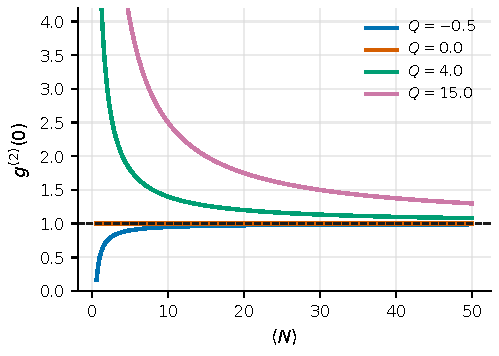
\includegraphics[width=0.86\linewidth]{figures/generated/chapter_04/ch04_mandel_q_g2.pdf}
\caption{在固定时间门内，Mandel \(Q\) 通过 \(g^{(2)}(0)=1+Q/\bar N\) 决定零延迟二阶相干。平均计数 \(\bar N\) 越低，同样的 \(Q\) 撬起的 \(g^{(2)}(0)-1\) 越大；把时间门加宽或平均更多模式，\(\bar N\) 增大、\(Q\) 被稀释，曲线逐渐回落到泊松基线 1。这解释了为什么报告二阶相关时必须同时注明门宽、模式数与平均计数。}
\label{fig:e07-mandel-q-g2}
\end{figure}

\section{多模稀释：为什么天文里的 excess 是小数而不是 1}
\label{sec:e07-multimode}

教科书上，单模热光的聚束峰堂堂正正是 \(g^{(2)}(0)=2\)，也就是 excess \(g^{(2)}(0)-1=1\)。可翻开任何一篇真实的天文强度干涉论文，你看到的峰高却是 \(10^{-3}\)、\(10^{-6}\) 这样卑微的小数。信号是不是丢了?没有。它是被\emph{多模平均}稀释了。这一节把稀释算清楚。

回忆第 \ref{chap:e05} 章：天文里"一个通道"几乎从来不是单单一个量子模式，而是 \(M\) 个独立模式的总和，\(M\simeq(\Delta t/\tau_c)(A\Omega/\lambda^2)N_{\rm pol}\)，可见光下轻易上千上万。现在把这句话的统计后果算出来。

设探测到的总计数 \(N\) 是 \(M\) 个\emph{独立、强度相近}的热光模式贡献之和，每个模式的平均计数为 \(m=\bar N/M\)。对单个热模，方差是 \(m+m^2\)（玻色--爱因斯坦，第 \ref{chap:e06} 章）。独立随机变量相加，\textbf{均值相加、方差也相加}（这是概率论里独立变量方差可加这一标准结论，我们直接引用）。于是总方差为
\[
  \sigma_N^2=\sum_{i=1}^{M}(m+m^2)=M m+M m^2
  =\underbrace{Mm}_{=\bar N}+M\Big(\frac{\bar N}{M}\Big)^2 .
\]
第一项 \(Mm=\bar N\) 就是总均值（散粒噪声那一份），第二项化简 \(M\cdot\bar N^2/M^2=\bar N^2/M\)。于是

\begin{equation}
  \sigma_N^2=\bar N+\frac{\bar N^{\,2}}{M}.
  \label{eq:e07-multimode-var}
\end{equation}
\begin{formulaexplain}
\(M\) 个独立热模平均后，方差的两部分：\(\bar N\) 是绕不开的散粒噪声，\(\bar N^2/M\) 是热光的额外"波动噪声"。模式越多（\(M\) 越大），第二项被摊得越薄，光就越像泊松。
\end{formulaexplain}

逐项交代：\(\bar N\) 是总平均计数（无量纲），\(M\) 是有效模式数（无量纲，\(\ge1\)），\(\bar N^2/M\) 是被 \(M\) 稀释后残留的超泊松涨落。现在把 \eqref{eq:e07-multimode-var} 塞进 Mandel \(Q\) 和 \(g^{(2)}(0)\)。先算 \(Q\)：
\[
  Q=\frac{\sigma_N^2-\bar N}{\bar N}
  =\frac{\bar N^2/M}{\bar N}=\frac{\bar N}{M}.
\]
再用换算式 \eqref{eq:e07-g2-q}：
\begin{equation}
  g^{(2)}(0)=1+\frac{Q}{\bar N}=1+\frac{1}{M}.
  \label{eq:e07-multimode-g2}
\end{equation}
\begin{formulaexplain}
\(M\) 个独立热模平均后，聚束峰高从单模的 \(g^{(2)}(0)-1=1\) 掉到 \(1/M\)。这一条 \(1/M\) 定律，就是天文强度干涉里 excess 总是小数的根源。
\end{formulaexplain}

这条 \(g^{(2)}(0)=1+1/M\) 干净得惊人，物理也清楚：\(M\) 个独立模式的强度涨落各自随机、互相抵消，平均下来强度越来越平稳，聚束这种"抱团"效应就被摊薄了 \(M\) 倍。\(M=1\) 给经典的 2；\(M=1000\) 给 \(1+10^{-3}\)；\(M=10^6\) 给 \(1+10^{-6}\)。这就是为什么天文 HBT 图上直接读到的从来不是雄伟的 2，而是要从海量事件对里刨出来的小数 excess。

那些 \(M\) 从哪来？逐个数（都在第 \ref{chap:e05} 章的模式计数框架里）：

\begin{itemize}
  \item \textbf{偏振（2 模）}：若不把偏振投影到单一通道，两个正交偏振各自是独立的热模，\(M_{\rm pol}\simeq2\)，一下就把理想峰从 2 压到 1.5。
  \item \textbf{空间散斑（speckle）}：被大气抖动（seeing）糊开的像、或耦合进粗光纤、或落在大像素上，会同时收进许多空间模式，\(M_{\rm sp}=A\Omega/\lambda^2\) 可以很大。
  \item \textbf{宽谱多频模}：滤光片越宽，带宽 \(\Delta\nu\) 内独立频率模式越多。
  \item \textbf{门宽 \(>\) 相干时间}：这是最狠的一项。可见光相干时间 \(\tau_c\sim1\,\mathrm{ps}\)，而最快探测器时间响应 \(\sim100\,\mathrm{ps}\)–\(1\,\mathrm{ns}\)，一个时间门里就压进了 \(\Delta t/\tau_c\sim10^2\)–\(10^3\) 个独立时间模式，单这一项就把 excess 压低两三个数量级。
\end{itemize}

代入一组真实标尺（取自恒星热光聚束实验）：中心波长约 \(7800\,\text{\AA}\)、最窄滤光片 \(10\,\text{\AA}\)，对应 \(\Delta\nu\simeq5\times10^{11}\,\mathrm{Hz}\)、相干时间 \(\tau_c\simeq1.6\)–\(2\,\mathrm{ps}\)；APD 单光子时间抖动约 \(500\,\mathrm{ps}\)，两只探测器的相对响应峰宽约 \(700\,\mathrm{ps}\)。光是"门宽/相干时间"这一项就贡献 \(M\sim700\,\mathrm{ps}/2\,\mathrm{ps}\sim350\) 倍稀释，再叠上偏振和空间模式，理想的 \(g^{(2)}(0)=2\) 就被压到观测峰 \(g^{(2)}(0)-1\sim10^{-3}\) 这个量级——实验里对三颗亮星测到的正是 \(10^{-3}\) 量级的聚束峰 \citep{2017MNRAS.472.4126G}。所以再强调一次：望远镜相关图上出现的 \(1+10^{-3}\)、\(1+10^{-6}\)，不是"没有聚束"，而是"聚束被 \(M\) 稀释"。要把 \(M\) 从数据里除干净，才能还原源本身的物理。这套稀释账，会在第 \ref{chap:e08} 章的 Siegert 关系和第 \ref{chap:e10} 章的空间强度干涉里反复用到。

\section{探测器不是理想的：效率、背景与死时间}
\label{sec:e07-nonideal}

到此为止我们假装探测器是完美的：每个到达的光子都被数到，没有噪声，数完立刻能数下一个。真实探测器三样都不满足。这一节把三种非理想性各讲一句物理，好在其中两种恰好能沿用我们已经建立的语言，第三种留个引子给第 \ref{chap:e13} 章。图 \ref{fig:e07-detection-loss} 把效率损耗与背景稀释这两条主线画在一起。

\paragraph{效率 η：损耗就像一块分束镜}
\label{sec:e07-efficiency}

真实探测器的量子效率（quantum efficiency）\(\eta<1\)：平均每 \(1/\eta\) 个到达的光子才被数到一个。怎样给这件事建模？有一个漂亮又准确的图像：\textbf{损耗完全等价于在光路上插一块透射率为 \(\eta\) 的分束镜（beamsplitter）}，透射的那一份 \(\eta\) 被数到，反射掉的 \(1-\eta\) 丢失，而分束镜的另一个入口漏进真空涨落。

这个图像的力量在于，它把"损耗"变成了"每个光子独立地以概率 \(\eta\) 存活"——这在概率论里叫\textbf{二项稀释}（binomial thinning）。而稀释一个分布有一条关键性质：它对\emph{泊松}分布是封闭的（泊松稀释后还是泊松），对超泊松分布则\emph{朝泊松方向拉}。

我们把这件事算到底，看看 Mandel \(Q\) 究竟怎么变。设某个时间门里\emph{到达}的光子数是随机变量 \(N\)（均值 \(\bar N\)、方差 \(\sigma_N^2\)），\emph{被数到}的计数是 \(M\)。二项稀释的意思是：给定 \(N\)，每个光子各自以概率 \(\eta\) 独立存活，于是条件分布是二项分布 \(M\mid N\sim\mathrm{Binomial}(N,\eta)\)，其条件均值与条件方差是二项分布的标准结果
\[
  \mathbb E[M\mid N]=\eta N,\qquad
  \operatorname{Var}(M\mid N)=N\,\eta(1-\eta).
\]
均值直接取期望：\(\bar M=\mathbb E[\eta N]=\eta\bar N\)。方差则要用\textbf{全方差公式}（law of total variance）\(\operatorname{Var}(M)=\mathbb E[\operatorname{Var}(M\mid N)]+\operatorname{Var}(\mathbb E[M\mid N])\)——它把总起伏拆成"每个 \(N\) 内部的二项抖动"和"\(N\) 本身在各门之间的起伏"两部分，是处理"随机个数里再随机存活"这类两层随机的标准工具。逐项代入：
\[
  \sigma_M^2
  =\underbrace{\mathbb E\big[N\,\eta(1-\eta)\big]}_{=\,\eta(1-\eta)\bar N}
  +\underbrace{\operatorname{Var}(\eta N)}_{=\,\eta^2\sigma_N^2}
  =\eta(1-\eta)\bar N+\eta^2\sigma_N^2 .
\]
第一项是损耗自己引入的二项散粒噪声，第二项是原起伏被 \(\eta^2\) 缩小后的残留。把 \(\bar M=\eta\bar N\) 和这个 \(\sigma_M^2\) 一起塞进 Mandel 参数的定义 \eqref{eq:e07-mandel-q}：
\[
  Q_M=\frac{\sigma_M^2-\bar M}{\bar M}
  =\frac{\eta(1-\eta)\bar N+\eta^2\sigma_N^2-\eta\bar N}{\eta\bar N}
  =\frac{\eta^2\sigma_N^2-\eta^2\bar N}{\eta\bar N}
  =\eta\,\frac{\sigma_N^2-\bar N}{\bar N}=\eta\,Q .
\]
中间那一步用到 \(\eta(1-\eta)\bar N-\eta\bar N=-\eta^2\bar N\)，把两项散粒噪声合并，剩下的正好整体提出一个 \(\eta\)。于是稀释把均值和方差过剩都按比例缩小，\(\bar N\to\eta\bar N\)，而
\[
  Q\ \longrightarrow\ \eta\,Q .
\]
一句话物理：

\begin{quote}
\textbf{损耗随机地删掉光子，把超泊松统计朝泊松零点拽。}\(\eta\to0\) 时任何光的计数都退化成泊松——这也是为什么效率极低的探测会"抹平"量子特征。
\end{quote}

但这里有一个救命的细节，务必记牢：\emph{归一化后的} \(g^{(2)}(0)\) 对损耗\textbf{免疫}。因为 \(Q\to\eta Q\) 而 \(\bar N\to\eta\bar N\)，代进 \eqref{eq:e07-g2-q}：
\[
  g^{(2)}(0)=1+\frac{\eta Q}{\eta\bar N}=1+\frac{Q}{\bar N}\quad(\text{不变}).
\]
分子分母上的 \(\eta\) 精确约掉。物理上这很合理：损耗只是随机地少数了一些光子，并不会改变"剩下的光子成对到达的\emph{倾向}"。这正是强度干涉即使在效率不高、光子稀少的天文条件下仍然可行的根本原因——\(g^{(2)}(0)-1\) 这个我们真正要测的量，不怕损耗。损耗伤的是\emph{信噪比}（少了光子就少了事件对，统计误差变大），而不是信号的\emph{数值}。

\paragraph{背景稀释：源光子只占一部分}
\label{sec:e07-background}

第二种非理想性是背景光：天光、月光、暗计数、邻近天体，都会在同一个通道里贡献与源无关的计数。设源光子只占总计数的比例为 \(f\)（source fraction，\(0<f\le1\)），其余 \(1-f\) 是不相关的背景。背景自己不带聚束峰（它是独立泊松的），而一次两光子符合要求\emph{两}个光子都来自源——每个各带一个因子 \(f\)。于是测到的 excess 被 \(f^2\) 压低：
\begin{equation}
  g^{(2)}_{\rm obs}(0)-1\simeq f^2\big[g^{(2)}_{\rm src}(0)-1\big].
  \label{eq:e07-background}
\end{equation}
\begin{formulaexplain}
背景把源信号按 \(f^2\) 稀释：两次点击都得是源光子才算数，各出一个 \(f\)。源只占一半（\(f=0.5\)）时，聚束峰就掉到原来的四分之一。
\end{formulaexplain}

逐项交代：\(f\) 是源计数占总计数的比例（无量纲），\(g^{(2)}_{\rm src}(0)\) 是源本身的二阶相干，\(g^{(2)}_{\rm obs}(0)\) 是掺了背景后测到的。这条 \(f^2\) 律和多模稀释的 \(1/M\) 是并列的两道关卡：一个来自"通道里混了多少无关模式"，一个来自"计数里混了多少无关背景"。做误差预算（第 \ref{chap:e15} 章会系统展开）时，两者都要老老实实乘进去。

\paragraph{死时间与后脉冲：留给第 13 章}
\label{sec:e07-deadtime}

第三种非理想性是探测器数完一个光子后，有一小段\emph{死时间}（dead time）不能再响应（单光子探测器常有 \(10\)–\(100\,\mathrm{ns}\)），以及触发后偶尔冒出的假计数（后脉冲，afterpulsing）。这两样会在\emph{零延迟附近}的自相关里挖坑、造假峰，恰好污染我们最想看的地方。它们不改变本章"数 \(n(n-1)\)"的基本规则，但会扭曲实测的相关峰形，需要专门的硬件对策（最常见的是用分束镜把光分到两只独立探测器做交叉相关，绕开单探测器的死时间）。这些属于探测器与事件表的硬件细节，我们留到第 \ref{chap:e13} 章专门处理，此处只提一句、按下不表。

\begin{figure}[tbp]
\centering
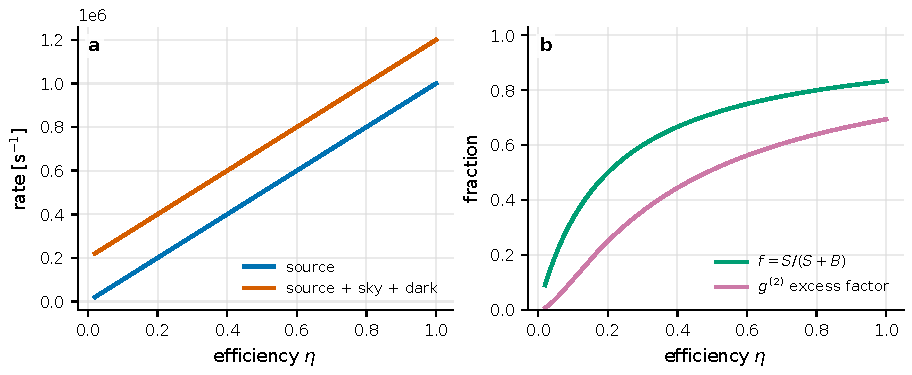
\includegraphics[width=0.85\linewidth]{figures/generated/chapter_03/ch03_detection_loss_background.pdf}
\caption{两种把观测统计朝泊松基线拉的非理想效应。效率损耗 \(\eta\) 等价于一块分束镜的二项稀释，随机删掉光子、把 Mandel \(Q\) 按 \(Q\to\eta Q\) 压向零点（但归一化后的 \(g^{(2)}(0)\) 不变）；背景稀释则把源信号按源光子占比 \(f\) 的平方 \(f^2\) 压低。二者与多模稀释 \(1/M\) 一起，构成天文强度相关信号被压成小数 excess 的三道关卡。}
\label{fig:e07-detection-loss}
\end{figure}

\section{本章要点}
\label{sec:e07-summary}

\begin{itemize}
  \item \textbf{探测就是吸收，所以数的是正规序。}单次点击率 \(\propto\langle\hat a^\dagger\hat a\rangle=\langle\hat n\rangle\)；两次符合点击率 \(\propto\langle\hat a^\dagger\hat a^\dagger\hat a\hat a\rangle=\langle\hat n(\hat n-1)\rangle\)。用 \([\hat a,\hat a^\dagger]=1\) 可精确证明 \(\hat a^\dagger\hat a^\dagger\hat a\hat a=\hat n(\hat n-1)\)。
  \item \textbf{\(n(n-1)\) 而非 \(n^2\)，是因为自配对被扣掉。}一个 START 和一个 STOP 必来自两次\emph{不同}吸收；\(N^2\) 里那 \(N\) 个"同一光子配自己"的假对被正规序自动减去，剩 \(N(N-1)\) 个真对，正是第 \ref{chap:e06} 章 \(b_2\) 分子的来历。
  \item \textbf{时间门 + Mandel \(Q\)。}把事件表切成宽 \(\Delta t\) 的门，数 \(N\)，得 \(\bar N=r\Delta t\)、\(\sigma_N^2\)；\(Q=(\sigma_N^2-\bar N)/\bar N\) 以泊松为零点：\(Q=0\) 泊松，\(Q>0\) 超泊松（热光），\(Q<0\) 亚泊松（非经典）。
  \item \textbf{一条恒等式连起两套语言。}由 \(\langle N(N-1)\rangle=\sigma_N^2+\bar N^2-\bar N\) 推得 \(g^{(2)}(0)=1+Q/\bar N\)。报告时必须同时给出 \(Q\)、门宽 \(\Delta t\)、模式数 \(M\)、平均计数 \(\bar N\)，缺一不可。
  \item \textbf{多模稀释的 \(1/M\) 律。}\(M\) 个独立热模平均后 \(\sigma_N^2=\bar N+\bar N^2/M\)，\(g^{(2)}(0)=1+1/M\)。偏振（2）、空间散斑、宽谱多频模、门宽 \(>\tau_c\) 都贡献 \(M\)，这就是天文 excess 常是 \(10^{-3}\)、\(10^{-6}\) 而非 1 的原因。
  \item \textbf{探测非理想。}效率 \(\eta\) 像分束镜，二项稀释把 \(Q\to\eta Q\)（超泊松被拉向泊松），但归一化的 \(g^{(2)}(0)\) 不变；背景把信号按 \(f^2\) 压低；死时间/后脉冲留待第 \ref{chap:e13} 章。
\end{itemize}

\medskip
\noindent\textbf{想一想。}
\begin{enumerate}
  \item 一束单模热光测得 \(g^{(2)}(0)=2\)。若把时间门宽从 \(1\,\mathrm{ps}\) 加宽到 \(1\,\mathrm{ns}\)（相干时间仍是 \(1\,\mathrm{ps}\)），有效时间模式数变成多少？此时 \(g^{(2)}(0)-1\) 大约掉到多少？
  \item 探测效率 \(\eta\) 从 \(0.5\) 掉到 \(0.05\)，测到的 \(g^{(2)}(0)-1\) 会变吗？Mandel \(Q\) 会变吗？分别说明为什么。
  \item 观测中源光子只占总计数的 \(f=1/3\)，其余是天光背景。若源本身是单模热光（\(g^{(2)}_{\rm src}(0)=2\)），你在这个通道里测到的 \(g^{(2)}_{\rm obs}(0)\) 大约是多少？
\end{enumerate}

\chapter{\texorpdfstring{相干函数 $g^{(1)}$、$g^{(2)}$ 与 Siegert 关系}{相干函数 g1、g2 与 Siegert 关系}}
\label{chap:e08}

\begin{chapteropening}
到这里，望远镜交给我们的已经不再是"一团亮度"，而是第 \ref{chap:e07} 章讲的那张\textbf{事件表}（event list）：一串带时间戳的"点击"。现在要问的，不再是"平均有多亮"，而是一个更微妙的问题——\emph{这些点击彼此之间，有没有关系？}如果两个探测器、两个时间门里的光子只是各自随机地到来，那么它们偶尔一起响一下，纯属巧合；可如果它们\emph{比巧合更常}一起响，或者\emph{比巧合更少}一起响，事件表里就藏着光场统计的指纹。本章要教你一套把"事件表"翻译成"光场统计"的语言：一阶相干 \(g^{(1)}\) 量的是电场的相位记忆，二阶相干 \(g^{(2)}\) 量的是光子结伴到达的倾向。而把这两者接通的，是本章的高潮——Siegert 关系。它会告诉你一件近乎魔法的事：只靠数强度涨落的"同步程度"，就能读出电场相干度的模平方。这正是后面强度干涉与成像的全部底气。
\end{chapteropening}

\section{为什么要给"相关"一个函数}
\label{sec:e08-why-correlation}

先把上一阶段的结论接住。第 \ref{chap:e02} 章告诉我们：光只在一个很短的相干时间 \(\tau_c\) 内"记得"自己的相位，可见光宽带下 \(\tau_c\) 短到皮秒；探测器却慢到百皮秒以上，一个时间门里平均了成百上千段互不相干的波列。第 \ref{chap:e06} 章又告诉我们，不同的光态（相干态、热态、数态）即便平均亮度一模一样，光子数的\emph{起伏}却天差地别。把这两条放在一起，一个自然的念头就冒出来了：\emph{既然一次曝光的总强度抹掉了这么多信息，我们能不能不看"总量"，改看"两次探测之间的呼应"？}

这正是相干函数（coherence function）的用武之地。它的思路极其朴素，和第 \ref{chap:e02} 章的自相关函数一脉相承：把光场（或光子流）和"延迟了 \(\tau\) 的自己"放在一起比较，看它们还有多像。区别只在于"比较什么"：

\begin{itemize}
  \item 若比较的是\textbf{电场振幅与相位}，得到的是一阶相干 \(g^{(1)}(\tau)\)——它回答"电场隔了 \(\tau\) 还记得多少相位"。振幅干涉（第 \ref{chap:e09} 章）用的就是它。
  \item 若比较的是\textbf{强度（光子到达）}，得到的是二阶相干 \(g^{(2)}(\tau)\)——它回答"两个探测事件是不是比随机情形更爱成对出现"。Hanbury Brown--Twiss（HBT）强度干涉用的就是它 \citep{1956Natur.177...27B}。
\end{itemize}

之所以要把"相关"写成一个\emph{关于延迟 \(\tau\) 的函数}，而不是一个数，是因为呼应的强弱随延迟变化：延迟很小时呼应最强，延迟拉长到超过相干时间，两次探测就彻底"失联"了。这条呼应随 \(\tau\) 衰减的曲线，它的\emph{高度}和\emph{宽度}里，分别编码着光的种类（热光还是激光）和光的谱宽（相干时间）。本章就是要把这两条曲线一根一根讲清楚，再把它们用一座桥——Siegert 关系——连起来。

\section{一阶相干：电场隔着 \texorpdfstring{$\tau$}{tau} 还记得多少相位}
\label{sec:e08-g1}

先看最容易想象的一阶。第 \ref{chap:e05} 章我们把探测面上的正频率电场写成算符 \(\hat E^{(+)}(t)\)（它只含湮灭算符 \(\hat a\)，作用是"减少一个光子"），它的厄米共轭 \(\hat E^{(-)}(t)\)（只含产生算符 \(\hat a^\dagger\)）是负频率部分。一阶相干函数定义为把两个时刻的场"相乘再平均"：

\begin{equation}
  G^{(1)}(t_1,t_2)=\big\langle \hat E^{(-)}(t_1)\,\hat E^{(+)}(t_2)\big\rangle,
  \qquad
  g^{(1)}(\tau)=\frac{G^{(1)}(t,t+\tau)}{G^{(1)}(t,t)} .
  \label{eq:e08-g1}
\end{equation}
\begin{formulaexplain}
\(G^{(1)}\) 是一阶场相关；\(\hat E^{(+)},\hat E^{(-)}\) 是正、负频率场算符；\(\langle\cdot\rangle\) 是量子态上的期望；\(g^{(1)}\) 是把它除以零延迟值后的归一化版本；\(\tau=t_2-t_1\) 是延迟。它测电场隔 \(\tau\) 还留多少相位记忆。
\end{formulaexplain}

逐个符号落实。\(G^{(1)}(t,t)=\langle\hat E^{(-)}(t)\hat E^{(+)}(t)\rangle\) 就是 \(t\) 时刻的平均强度（正实数，带强度量纲），所以归一化后的 \(g^{(1)}\) 是无量纲的复数。若光场是\emph{平稳的}（statistically stationary，统计性质不随绝对时间漂移，这是稳定光源的常态），相关只依赖延迟 \(\tau\)，与起点 \(t\) 无关，于是 \(g^{(1)}\) 只是 \(\tau\) 的函数。它的模 \(|g^{(1)}(\tau)|\) 落在 \([0,1]\) 之间，物理含义一句话就能抓住：

\begin{itemize}
  \item \(|g^{(1)}(\tau)|\to1\)：延迟 \(\tau\) 之后的电场，仍和原来的电场步调一致、相位可预测——\textbf{相干}。把它和延迟前的自己叠加，会拉出清晰的干涉条纹。
  \item \(|g^{(1)}(\tau)|\to0\)：电场已经把 \(\tau\) 之前的相位忘得干干净净——\textbf{失忆}。此时叠加得到的是一片糊掉的、没有条纹的亮度。
\end{itemize}

这正是第 \ref{chap:e02} 章自相关函数 \(\Gamma(\tau)\) 的"电场版"：\(g^{(1)}(\tau)\) 从峰值 1 衰减到 0 的宽度，就是相干时间 \(\tau_c\)。而 \(\tau_c\) 由谱宽定，回忆第 \ref{chap:e02} 章的两条式子：

\begin{equation}
  \Delta\nu\simeq\frac{c\,\Delta\lambda}{\lambda^2},
  \qquad
  \tau_c\simeq\frac{1}{\Delta\nu}\simeq\frac{\lambda^2}{c\,\Delta\lambda}.
  \label{eq:e08-tauc}
\end{equation}
\begin{formulaexplain}
\(\Delta\nu\) 是频率带宽（Hz），\(\Delta\lambda\) 是波长带宽，\(\lambda\) 是中心波长，\(c\) 是光速，\(\tau_c\) 是相干时间（s）。它把"滤光片有多窄"直接换算成"电场相位记忆有多久"。
\end{formulaexplain}

代进真实数字体会一下量级。取一片"很窄"的滤光片：中心波长 \(\lambda=780\,{\rm nm}\)、带宽 \(\Delta\lambda=1\,{\rm nm}\)。先算频率带宽（用 CGS，\(c=3\times10^{10}\,{\rm cm\,s^{-1}}\)，\(\lambda=7.8\times10^{-5}\,{\rm cm}\)，\(\Delta\lambda=10^{-7}\,{\rm cm}\)）：
\[
  \Delta\nu\simeq\frac{(3\times10^{10})(10^{-7})}{(7.8\times10^{-5})^2}
  =\frac{3\times10^{3}}{6.1\times10^{-9}}
  \approx4.9\times10^{11}\,{\rm Hz},
\]
于是
\[
  \tau_c\simeq\frac{1}{4.9\times10^{11}\,{\rm Hz}}\approx2\times10^{-12}\,{\rm s}=2\,{\rm ps}.
\]
也就是说，即便隔着一片 1 纳米的窄带滤光片，恒星热光的电场也只记得自己约 2 皮秒的相位，然后就翻篇了。这个 2 ps 会在本章反复出现，并直接决定后面强度相关峰有多窄、被稀释多少倍。

\section{二阶相干：光子是否喜欢结伴到达}
\label{sec:e08-g2}

把问题从"电场是否还记得相位"换成"两个探测事件是否相关"，就进入二阶。量子光电探测理论（第 \ref{chap:e07} 章）给出的定义，是四个场算符按一种特定次序排好后取平均：

\begin{equation}
  G^{(2)}(t_1,t_2)=\big\langle
    \hat E^{(-)}(t_1)\,\hat E^{(-)}(t_2)\,\hat E^{(+)}(t_2)\,\hat E^{(+)}(t_1)
  \big\rangle,
  \qquad
  g^{(2)}(\tau)=\frac{G^{(2)}(t,t+\tau)}{G^{(1)}(t,t)\,G^{(1)}(t+\tau,t+\tau)} .
  \label{eq:e08-g2-field}
\end{equation}
\begin{formulaexplain}
\(G^{(2)}\) 是二阶场相关；四个算符里两个产生（\(\hat E^{(-)}\)）全排在左边、两个湮灭（\(\hat E^{(+)}\)）全排在右边，这叫\textbf{正规序}（normal order）；至于内外那层嵌套，是按时间配对的（\(t_1\) 一对在最外层、\(t_2\) 一对在里层），保证"先在 \(t_1\) 吸收、再在 \(t_2\) 吸收"的时间序。分母是两个时刻各自的平均强度之积；\(g^{(2)}\) 是归一化结果。它测光子是否倾向成对到达。
\end{formulaexplain}

这条式子值得逐项慢慢读，因为每一项都对应事件表里一个能数出来的东西。

\textbf{为什么是这个奇怪的算符次序？}第 \ref{chap:e07} 章讲过，探测器"数"的是\emph{吸收}一个光子的事件，每吸收一个就用掉一个湮灭算符 \(\hat E^{(+)}\)。要在 \(t_1\) 和 \(t_2\) 两个时刻各探到一个光子，就要连用两个湮灭算符 \(\hat E^{(+)}(t_2)\hat E^{(+)}(t_1)\) 作用在态上，得到态矢 \(\hat E^{(+)}(t_2)\hat E^{(+)}(t_1)|\psi\rangle\)；这个联合探测的概率正是它的模平方 \(\big|\hat E^{(+)}(t_2)\hat E^{(+)}(t_1)|\psi\rangle\big|^2\)，展开来就是把两个产生算符原样搬到左边。于是产生算符全排在左边、湮灭算符全排在右边——这就是正规序，它保证我们数的是\emph{两个不同的吸收事件}，而不是同一个光子和自己配对的假项。至于公式里"外/内"那层嵌套，纯粹来自时间配对：带 \(t_1\) 的一对（一个产生、一个湮灭）在最外层，带 \(t_2\) 的一对在里层，锁定"先在 \(t_1\) 吸收、再在 \(t_2\) 吸收"的时间顺序，与"产生在左、湮灭在右"是两件不同的事，别把它们混为一谈。这一点在第 \ref{chap:e07} 章的阶乘矩 \(\langle N(N-1)\rangle\) 里已经埋下伏笔：探测器允许的是不同光子组成的有序对。

\textbf{分母是什么？}分母 \(G^{(1)}(t,t)\,G^{(1)}(t+\tau,t+\tau)=\langle I(t)\rangle\langle I(t+\tau)\rangle\)，是"假设两个探测完全独立时，随机符合应该有多少"的基线。换句话说，如果两个时刻的光子毫不相干，各自按自己的平均率随机到来，那么它们碰巧一起被探到的联合率，就是两个平均率相乘。

\textbf{分子是什么？}分子是真实的\emph{共同}探测强度。把它除以那条"独立时的随机符合基线"，\(g^{(2)}\) 就成了一个无量纲的\emph{相对过量}：

\begin{itemize}
  \item \(g^{(2)}(\tau)=1\)：真实符合恰好等于随机基线，光子的到来彼此独立。理想激光（相干态，第 \ref{chap:e06} 章）就是这样——它给出泊松（Poisson）计数，\(g^{(2)}=1\)。
  \item \(g^{(2)}(0)>1\)：零延迟附近的光子对\emph{比随机更多}，光子爱扎堆，叫\textbf{聚束}（bunching）。理想单模热光给出漂亮的 \(g^{(2)}(0)=2\)。
  \item \(g^{(2)}(0)<1\)：零延迟符合被\emph{压低}，光子彼此回避，叫\textbf{反聚束}（antibunching）。这一条无法由任何正定的经典强度涨落解释，是单光子源、共振荧光的标准\emph{非经典}判据 \citep{1977PhRvL..39..691K}。
\end{itemize}

理想单模热光为什么恰好是 2？物理图像在第 \ref{chap:e06} 章已经埋好：热光的电场是许多随机相位的小贡献叠加，瞬时强度会形成随机的明暗斑纹；探测器在"亮斑"里更容易接连记录多个光子，于是零延迟附近符合升高。而 2 这个具体数字，正是下一节 Siegert 关系在 \(\tau=0\) 处的直接推论——先记住这个悬念。

在工程估算里，人们常把同一件事写成连续强度的形式：

\begin{equation}
  g^{(2)}(\tau)=\frac{\big\langle I(t)\,I(t+\tau)\big\rangle}{\big\langle I(t)\big\rangle^2}.
  \label{eq:e08-g2-classical}
\end{equation}
\begin{formulaexplain}
\(I(t)\) 是强度（或正比于它的探测电流、计数率）；分子是两时刻强度的共同涨落；分母是平均强度的平方（用了平稳性，两个时刻的平均相同）。这是二阶相干的"经典写法"，便于估算。
\end{formulaexplain}

这行式子方便，但埋着一个必须点破的\textbf{陷阱}：\(I(t)\) 到底是哪一个强度？它可以是光场理想的\emph{瞬时}强度，也可以是探测器输出的电流、TDC 记录的事件率或采样后的 ADC 值。这两者天差地别——后者已经被探测器几纳秒的响应\emph{卷积}过了。如果你把一个被 4 ns 电子响应抹平后的 \(I(t)\) 代进式 \eqref{eq:e08-g2-classical}，得到的是"响应之后"的 \(g^{(2)}\)，而不是光场本身皮秒宽度的相关峰。许多天文强度相关信号并不是"没有聚束"，而是那个本该高达 2 的峰，被有限时间响应、多模式和背景光压低到了 \(10^{-3}\)、\(10^{-6}\) 甚至更小（第 \ref{sec:e08-telescope} 节会把这笔账算清）。所以每次写下式 \eqref{eq:e08-g2-classical}，都要在心里追问一句：这个 \(I\)，被卷积过了吗？

\section{Siegert 关系：从强度相关读出场相干的模平方}
\label{sec:e08-siegert}

现在到本章的高潮。前两节各自定义了 \(g^{(1)}\)（场相位记忆）和 \(g^{(2)}\)（光子成对倾向），它们看起来是两码事——一个关于相位，一个关于强度。HBT 实验的核心奇迹在于：对\textbf{高斯混沌光}（Gaussian chaotic light，即热光这类由大量独立小贡献随机叠加而成的光），这两者之间存在一座精确的桥。跨过这座桥，你就能只用"数强度涨落"这种探测器做得到的测量，反推出电场相干度——一个探测器本来"看不见"的相位信息。

\paragraph{关键工具：高斯矩定理（Wick 定理）}
\label{sec:e08-gaussian-moment}

桥的桥墩是一条统计学定理，我们先把它单独讲清楚，绝不默默代入。

热光的电场 \(E(t)\) 是海量独立辐射子（原子、电子）贡献的相位随机叠加。由\textbf{中心极限定理}（central limit theorem，大量独立随机量之和趋于高斯分布），复电场 \(E=E_r+iE_i\) 近似服从\emph{零均值圆对称复高斯}（zero-mean circular complex Gaussian）分布。"圆对称"这个词很关键，它意味着电场的相位在 \([0,2\pi)\) 上完全均匀，由此可以推出一个我们马上要用的性质：

\begin{equation}
  \langle E(t_1)\,E(t_2)\rangle=0,
  \qquad\text{但}\qquad
  \langle E^*(t_1)\,E(t_2)\rangle=G^{(1)}(t_1,t_2)\neq0.
  \label{eq:e08-circular}
\end{equation}
\begin{formulaexplain}
两个电场（都不带星号）相乘平均为零，是因为它们的总相位随机、正负相消；一个带星号、一个不带，相位相消后才留下非零的相关。这是圆对称高斯场的定义性性质。
\end{formulaexplain}

对这种场，\textbf{高斯矩定理}（Gaussian moment theorem，在概率论里叫 Isserlis 定理，在量子场论里叫 Wick 定理）说：\emph{任意高阶矩都可以拆成二阶矩（两两配对）之和，遍历所有配对方式}。而由式 \eqref{eq:e08-circular}，只有"一个星号配一个不带星号"的配对才不为零，其余全部消失。这就是我们要用的全部内容——它不是近似，是零均值圆高斯分布的严格代数事实。

\paragraph{把四阶矩拆开}
\label{sec:e08-factorize}

现在动手。二阶相干的分子（用经典强度写，\(I=E^*E\)）是一个四阶矩：
\[
  \big\langle I(t)\,I(t+\tau)\big\rangle
  =\big\langle E^*(t)\,E(t)\,E^*(t+\tau)\,E(t+\tau)\big\rangle .
\]
四个场里有两个带星号（\(E^*(t),E^*(t+\tau)\)）、两个不带星号（\(E(t),E(t+\tau)\)）。按高斯矩定理，把它们两两配对，只保留"星号配非星号"的项。两种合法配对：

\emph{配对一}：\(E^*(t)\) 配 \(E(t)\)，\(E^*(t+\tau)\) 配 \(E(t+\tau)\)——各自"就地"配对。给出
\[
  \langle E^*(t)E(t)\rangle\,\langle E^*(t+\tau)E(t+\tau)\rangle
  =\langle I(t)\rangle\,\langle I(t+\tau)\rangle=\langle I\rangle^2 .
\]

\emph{配对二}：\(E^*(t)\) 配 \(E(t+\tau)\)，\(E^*(t+\tau)\) 配 \(E(t)\)——"交叉"配对。给出
\[
  \langle E^*(t)E(t+\tau)\rangle\,\langle E^*(t+\tau)E(t)\rangle
  =G^{(1)}(\tau)\,G^{(1)}(-\tau)
  =G^{(1)}(\tau)\,\big[G^{(1)}(\tau)\big]^*
  =\big|G^{(1)}(\tau)\big|^2 .
\]
（这里用了平稳场的对称性 \(G^{(1)}(-\tau)=[G^{(1)}(\tau)]^*\)。）两项相加：

\begin{equation}
  \big\langle I(t)\,I(t+\tau)\big\rangle=\langle I\rangle^2+\big|G^{(1)}(\tau)\big|^2 .
  \label{eq:e08-G2-factor}
\end{equation}
\begin{formulaexplain}
左边是可测的强度相关；右边第一项 \(\langle I\rangle^2\) 是"独立时的随机基线"，第二项 \(|G^{(1)}(\tau)|^2\) 是电场相干度贡献的额外涨落。四阶矩就此被拆成两个二阶矩之和。
\end{formulaexplain}

把两边除以 \(\langle I\rangle^2\)，并注意 \(|g^{(1)}(\tau)|^2=|G^{(1)}(\tau)|^2/\langle I\rangle^2\)，立刻得到理想形式的 \textbf{Siegert 关系}：
\[
  g^{(2)}(\tau)=1+\big|g^{(1)}(\tau)\big|^2 \qquad(\text{理想单一时空偏振模式}).
\]
在 \(\tau=0\)，\(|g^{(1)}(0)|=1\)，于是 \(g^{(2)}(0)=1+1=2\)。上一节那个"热光为什么恰好是 2"的悬念，到这里揭晓：那个 2，就是随机基线的 1，加上电场完全相干时贡献的 1。

\paragraph{装进真实望远镜：可见度因子 \texorpdfstring{$\zeta$}{zeta}}
\label{sec:e08-zeta}

真实探测从来没有"单一时空偏振模式"这么理想。未分偏振的光至少混了两个偏振、宽光谱里有多个频率模式、大气抖动（seeing，星像被湍流糊开的现象）造出的像里有多个空间斑、背景光还掺进来稀释——这些都会把那个理想的 1 压低。把所有这些稀释因素打包成一个\textbf{可见度因子}（visibility factor）\(\zeta\)，Siegert 关系写成本章的招牌形式：

\begin{equation}
  \boxed{\,g^{(2)}(\tau)=1+\zeta\,\big|g^{(1)}(\tau)\big|^2\,},
  \qquad 0<\zeta\le1 .
  \label{eq:e08-siegert}
\end{equation}
\begin{formulaexplain}
\(g^{(2)}-1\) 是强度相关的过量；\(|g^{(1)}|^2\) 是一阶场相干度的模平方；\(\zeta\) 收集\emph{真实相关}层面的稀释——模式数、偏振、背景，理想单模时 \(\zeta=1\)。有限时间响应\emph{不}算进 \(\zeta\)，它在第 \ref{sec:e08-telescope} 节以卷积单独处理。这是 HBT 从强度相关读出场相干模平方的核心桥梁。
\end{formulaexplain}

逐项交代 \(\zeta\) 的来源：未分偏振热光已经有 \(M_{\rm pol}\simeq2\) 个偏振模式，把峰高从 2 拉到 1.5（即 \(\zeta\simeq1/2\)）；多个空间斑、多个频率模式各自再乘一个 \(1/M\)；若源光子只占两个通道总计数的比例分别为 \(f_A,f_B\)（其余是背景），相关幅度还要近似乘上 \(f_Af_B\)。这些因子的乘积可以轻易把 \(\zeta\) 压到 \(10^{-3}\) 以下——这就是为什么天文 HBT 图上看到的是 \(g^{(2)}-1\) 的小数，而不是教科书里干净的 1。

式 \eqref{eq:e08-siegert} 的意义怎么强调都不过分：\emph{左边是事件表能直接测的强度相关，右边的 \(g^{(1)}\) 是电场相干度}。而 \(g^{(1)}\) 我们有两条独立的路子拿到——它是谱线形状的傅里叶变换（维纳--辛钦定理，第 \ref{chap:e02} 章），也是振幅干涉仪测到的条纹可见度（第 \ref{chap:e09} 章）。于是强度涨落的"同步程度"，就换算成了电场相干度的模平方。

\begin{figure}[tbp]
\centering
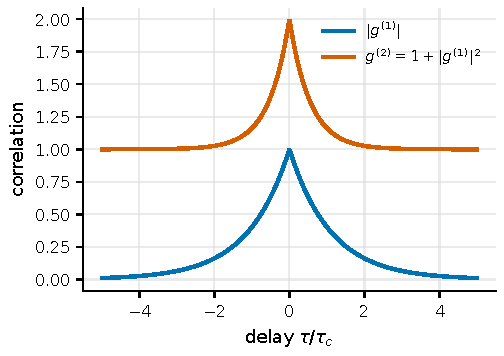
\includegraphics[width=0.86\linewidth]{figures/generated/chapter_04/ch04_siegert_relation.pdf}
\caption{Siegert 关系把一阶场相干的衰减，转化成二阶强度聚束峰。若 \(|g^{(1)}(\tau)|\) 随延迟以相干时间 \(\tau_c\) 衰减，则 \(g^{(2)}(\tau)-1\) 按 \(|g^{(1)}(\tau)|^2\) 衰减，并在大延迟回到无相关值 0；零延迟峰高在理想单模时为 1，真实观测还要乘上可见度因子 \(\zeta\)（模式数、偏振、背景；有限时间响应不含在 \(\zeta\) 内，另由卷积处理，见第 \ref{sec:e08-telescope} 节）。}
\label{fig:e08-siegert}
\end{figure}

\paragraph{谱形决定峰形；相干态是例外}
\label{sec:e08-shapes}

既然 \(g^{(1)}(\tau)\) 是谱线的傅里叶变换，那么\emph{谱线长什么样，聚束峰就长什么样}。三个常见谱形值得记住：

\begin{itemize}
  \item \textbf{矩形谱}（带宽 \(\Delta\nu\) 内平顶）：傅里叶变换是 sinc 函数，故 \(|g^{(1)}(\tau)|^2\propto{\rm sinc}^2(\Delta\nu\,\tau)\)——峰带旁瓣。
  \item \textbf{洛伦兹谱}（Lorentzian，如碰撞展宽或自然线宽）：\(|g^{(1)}(\tau)|=e^{-|\tau|/\tau_c}\) 是双边指数衰减，故 \(g^{(2)}-1\propto e^{-2|\tau|/\tau_c}\)——尖顶。
  \item \textbf{高斯谱}（Gaussian，如多普勒展宽）：傅里叶变换仍是高斯，故 \(|g^{(1)}(\tau)|^2\) 也是高斯——圆顶。
\end{itemize}

反过来用，就是一门实验技术：测出 \(g^{(2)}(\tau)\) 峰的\emph{宽度}，就能反推谱线宽度。对于像 \(\eta\) Carinae 附近那些天体激光候选谱线，普通光谱仪很难做到光谱分辨本领 \(R\equiv\lambda/\Delta\lambda\sim10^8\)（无量纲），而纳秒级的强度相关却能对 MHz 到 GHz 的线宽给出独立约束 \citep{2005NewA...10..361J,2008AIPC..984..216D,2014ApJ...789L..10T}。

但必须把\textbf{适用边界}钉死：Siegert 关系是\emph{高斯混沌光专属}的。理想相干态（激光）明明有很长的一阶相干（\(g^{(1)}\) 长程不衰减），可它的 \(g^{(2)}\equiv1\)——绝不满足 \(1+|g^{(1)}|^2\)。原因正是圆高斯假设不成立：相干态不是大量随机相位的叠加，它的场没有那种明暗斑纹起伏。同理，反聚束光、压缩光、单光子源、强非平稳脉冲，以及少数几个相干子源的叠加，都会打破式 \eqref{eq:e08-siegert}。天文上更常见的是混合场——许多非热小源平均后近似热光，或热连续谱上叠加一条窄非热线——用 Siegert 关系前，务必先确认光的"混沌"血统。

\section{从理想相关到望远镜里的估计量}
\label{sec:e08-telescope}

理想的 \(g^{(2)}\) 峰又窄又高（皮秒宽、峰高 1）。可探测器不是无限快的，它测到的是理想相关与\emph{仪器响应}的卷积：

\begin{equation}
  g_{\rm obs}^{(2)}(\tau)-1=\int_{-\infty}^{+\infty}
  \big[g_{\rm true}^{(2)}(\tau')-1\big]\,R_{\Delta t}(\tau-\tau')\,{\rm d}\tau',
  \label{eq:e08-response-conv}
\end{equation}
\begin{formulaexplain}
\(g_{\rm true}^{(2)}\) 是光场本征相关；\(g_{\rm obs}^{(2)}\) 是观测到的；\(R_{\Delta t}\) 是面积归一化为 1 的仪器响应函数（由探测器 jitter、电子带宽、采样窗口、分析 bin 共同决定）；\(\tau'\) 是积分变量。卷积会把窄峰拉宽、压低，但守住峰的面积。
\end{formulaexplain}

这里藏着一个容易误解的事实：卷积\emph{守面积、不守峰高}。一个面积固定的窄峰，被一个宽得多的响应抹开后，峰会变矮变胖。若内禀峰宽 \(\tau_c\) 远小于有效响应宽度 \(\Delta t_{\rm eff}\)，那么峰高近似按 \(\tau_c/\Delta t_{\rm eff}\) 这个比例被稀释。把这项时间稀释和上一节的模式、背景稀释合在一起，就得到望远镜里相关峰高的\emph{误差预算式}：

\begin{equation}
  C_{\rm obs}\equiv g_{\rm obs}^{(2)}(0)-1
  \simeq C_{\rm true}\,\frac{\tau_c}{\Delta t_{\rm eff}}\,\frac{1}{M}\,f_A f_B,
  \label{eq:e08-contrast}
\end{equation}
\begin{formulaexplain}
\(C_{\rm obs}\) 是观测峰高，\(C_{\rm true}\) 是理想峰高（单模热光为 1）；\(\tau_c/\Delta t_{\rm eff}\) 是时间稀释；\(M=M_{\rm pol}M_{\rm sp}\) 是偏振与空间模式数；\(f_A,f_B\) 是两通道里源光子占总计数的比例（背景稀释）。这是数量级公式，精确分析要把实测响应、谱形 \(|g^{(1)}|^2\)、背景一起放进模型。
\end{formulaexplain}

\begin{figure}[tbp]
\centering
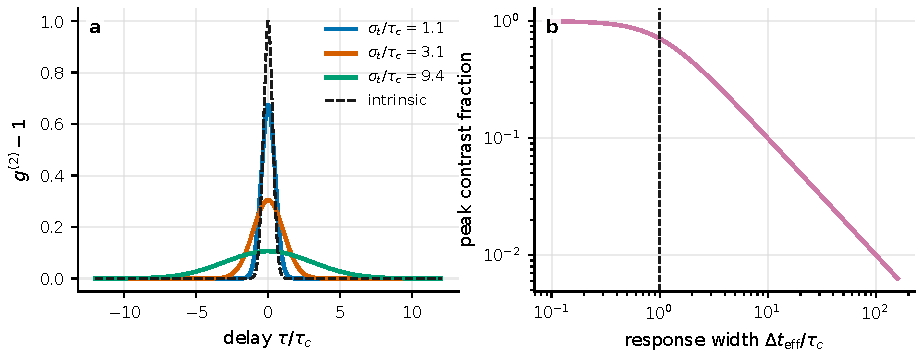
\includegraphics[width=0.95\linewidth]{figures/generated/chapter_04/ch04_response_convolution.pdf}
\caption{有限时间响应把窄的热光聚束峰拉宽、压低。左图虚线是内禀皮秒量级峰，实线是被不同响应宽度卷积后的观测峰；右图显示当 \(\Delta t_{\rm eff}\gg\tau_c\) 时，零延迟峰高近似按 \(\tau_c/\Delta t_{\rm eff}\) 下降——面积守住了，峰高被稀释。}
\label{fig:e08-response}
\end{figure}

\textbf{代进真实标尺：Guerin 恒星聚束实验。}\ Guerin 等人用 1 米望远镜、多模光纤、分束器、两只雪崩光电二极管（APD）和延迟直方图，测到了恒星的热光聚束 \citep{2017MNRAS.472.4126G}。他们的参数是一组极好的量级练习：中心波长约 \(7800\,\text{\AA}\)，最窄滤光片带宽 \(10\,\text{\AA}\)。先算相干时间（同式 \eqref{eq:e08-tauc}）：\(\Delta\nu\simeq c\Delta\lambda/\lambda^2\approx5\times10^{11}\,{\rm Hz}\)，故 \(\tau_c\simeq2\,{\rm ps}\)。而两个探测器的相对响应峰宽约 \(\Delta t_{\rm eff}\approx700\,{\rm ps}\)（单只 APD 的时间 jitter 约 500 ps）。理想热光 \(C_{\rm true}=1\)，仅时间稀释一项就给出 \(\tau_c/\Delta t_{\rm eff}\approx2/700\approx3\times10^{-3}\)。这已经是峰高的主导因子；在它之外，还要再乘上一个 \(\mathcal O(1)\) 的形状/模式系数——洛伦兹内禀峰与近高斯响应卷积后，零延迟峰高相对"面积除以响应宽"这一粗估会有一个约 \(0.7\) 的峰形折扣，加上残余的偏振/模式与背景稀释——把预期峰高压到

\[
  C_{\rm obs}\approx(2\text{--}3)\times10^{-3}\quad(\text{量级估计}),
\]

与实验室热源实测 \((2.01\pm0.09)\times10^{-3}\)、以及三颗亮星给出的约 \(1.8\)--\(2.0\times10^{-3}\) 的峰做数量级比较，符合得很好。结论一句话：望远镜相关图上直接冒出来的，绝不是教科书的 \(g^{(2)}(0)=2\)，而是 \(1+10^{-3}\)、\(1+10^{-6}\) 乃至更小的过量。看得见这个小数，靠的是海量事件对的累积。

\paragraph{延迟直方图：把事件表变成相关函数}
\label{sec:e08-histogram}

那么在事件表里，\(g^{(2)}\) 具体怎么估出来？答案是\textbf{延迟直方图}（delay histogram）。取两个通道 \(A,B\)，把每一对事件的时间差 \(t_{B,j}-t_{A,i}\) 都算出来，扔进宽为 \(\delta\tau\) 的延迟 bin 里累计：

\begin{equation}
  H_{AB}(\tau_m)=\sum_{i\in A}\sum_{j\in B}
  \mathbf{1}\!\left(\tau_m-\tfrac{\delta\tau}{2}\le t_{B,j}-t_{A,i}<\tau_m+\tfrac{\delta\tau}{2}\right),
  \label{eq:e08-histogram}
\end{equation}
\begin{formulaexplain}
\(H_{AB}(\tau_m)\) 是延迟落在第 \(m\) 个 bin（中心 \(\tau_m\)、宽 \(\delta\tau\)）里的事件对数；\(\mathbf 1(\cdot)\) 是示性函数，落进窗内取 1、否则取 0；双重求和遍历两通道所有事件对。它把事件表直接变成相关函数的原始计数。
\end{formulaexplain}

要把这个原始计数归一化成"无相关时等于 1"的 \(g^{(2)}\)，就除以随机符合的期望。设两通道平均计数率 \(r_A,r_B\)，总有效观测时长（live time）\(T\)：

\begin{equation}
  \widehat g^{(2)}_{AB}(\tau_m)=\frac{H_{AB}(\tau_m)}{r_A\,r_B\,\delta\tau\,T}.
  \label{eq:e08-estimator}
\end{equation}
\begin{formulaexplain}
\(\widehat g^{(2)}_{AB}\) 是二阶相关的估计量；分母 \(r_Ar_B\,\delta\tau\,T\) 是同样时长、同样 bin 宽、同样计数率下的随机符合期望。分子分母都是"对数"，比值无量纲，且在无相关时自动等于 1。
\end{formulaexplain}

分母的道理很直白：\(A\) 通道一共有 \(r_AT\) 个事件，对每个 \(A\) 事件，一个 \(B\) 事件恰好落进它 \(\delta\tau\) 窗口的概率是 \(r_B\delta\tau\)，两者相乘就是期望的随机符合数。实际分析常常不用这条解析分母，而是用大时间偏移、不同观测段、偏振错配或 off-source 通道构造一条参考直方图 \(H_{\rm ref}\)，再取比值——这样能吸收 TDC bin 宽不均、电子串扰、慢变透明度等系统效应。

\begin{figure}[tbp]
\centering
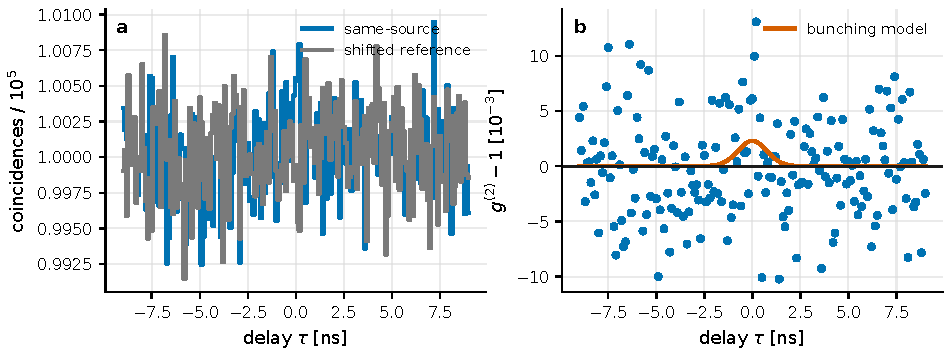
\includegraphics[width=0.95\linewidth]{figures/generated/chapter_04/ch04_delay_histogram_estimator.pdf}
\caption{延迟直方图估计量的结构。左图中同源事件对的直方图，在零延迟附近比移位的参考直方图多出很小的符合数；右图把差值按随机符合数归一化后得到 \(g^{(2)}-1\)，峰值只有 \(10^{-3}\) 量级。真实观测还要叠加死时间、背景和响应函数修正。}
\label{fig:e08-delay-hist}
\end{figure}

\paragraph{统计误差：一切都靠数够事件对}
\label{sec:e08-shotnoise}

估计量的精度从哪来？主要来自随机符合对数的散粒噪声。若某个延迟 bin 里随机符合数为 \(N_{\rm pair}\)，它是泊松涨落（第 \ref{chap:e03} 章），标准差 \(\sqrt{N_{\rm pair}}\)，相对误差就是

\begin{equation}
  \sigma\!\left[\widehat g^{(2)}(\tau)\right]\sim\frac{1}{\sqrt{N_{\rm pair}}}.
  \label{eq:e08-shotnoise}
\end{equation}
\begin{formulaexplain}
\(\sigma[\widehat g^{(2)}]\) 是相关估计量的统计误差；\(N_{\rm pair}=r_Ar_B\,\delta\tau\,T\) 是该 bin 的随机符合对数。要把误差压到 \(10^{-3}\) 以下的信号之下，就得积累巨量事件对。
\end{formulaexplain}

代进一组数字体会难度。取两个 \(r=10^{6}\,{\rm s^{-1}}\) 的通道、\(\delta\tau=100\,{\rm ps}=10^{-10}\,{\rm s}\)、\(T=1\,{\rm hr}=3600\,{\rm s}\)：
\[
  N_{\rm pair}=r_Ar_B\,\delta\tau\,T
  =(10^6)(10^6)(10^{-10})(3600)
  =3.6\times10^{5},
\]
故单 bin 统计误差 \(\sigma\sim1/\sqrt{3.6\times10^5}\approx1.7\times10^{-3}\)。这几乎和 Guerin 的信号 \(2\times10^{-3}\) 同量级——也就是说，一小时、单个延迟 bin 还远远不够，勉强只有 \(1\sigma\)。要把误差压到 \(10^{-4}\)，需要 \(N_{\rm pair}\sim10^{8}\)，也就是把事件对数从 \(3.6\times10^5\) 再积累约 \(300\) 倍（\(10^8/3.6\times10^5\approx278\)）。注意这 300 倍在两条路径上的标度并不相同：\(N_{\rm pair}\propto T\) 对曝光是线性的，故曝光时间需延长约 \(300\) 倍；而 \(N_{\rm pair}\propto r_Ar_B\) 对计数率是平方的，故两通道计数率各提高约 \(\sqrt{300}\approx17\) 倍即可（本章第 3 道"想一想"考的正是这个 \(r^2\) 标度）。当然也可以两者结合，或把聚束峰跨越的多个 bin 一起拟合（峰不止一个 bin 宽，可以联合利用）。这也提醒一个上限：当系统相关（TDC 串扰、背景归一化残差）停在 \(10^{-3}\) 量级时，继续加曝光并不能替代对这些系统项的修正。现代 VERITAS 与 MAGIC 强度干涉正是把这一思想，用离线相关、GPU/FPGA 相关器和多基线平均，推广到了空间尺度 \citep{2020NatAs...4.1164A,2024MNRAS.529.4387A}。

\section{前瞻：三阶相关与闭合相位}
\label{sec:e08-g3}

二阶相关只动用光子\emph{对}。如果同时保留三个望远镜（或三个通道），就能定义三阶强度相关：

\begin{equation}
  g^{(3)}_{123}=\frac{\big\langle I_1 I_2 I_3\big\rangle}
  {\big\langle I_1\big\rangle\big\langle I_2\big\rangle\big\langle I_3\big\rangle}.
  \label{eq:e08-g3}
\end{equation}
\begin{formulaexplain}
\(g^{(3)}_{123}\) 是三通道归一化强度相关；\(I_1,I_2,I_3\) 是三个望远镜的强度；分母是随机三重符合基线。它把统计对象从"光子对"推广到"光子三元组"。
\end{formulaexplain}

对高斯混沌光，同样用高斯矩定理把六阶矩拆开（这次是三个不带星号、三个带星号的场两两配对，"星号配非星号"的合法配对共 \(3!=6\) 个：其中 3 个把 \(I_i\) 就地配成 \(|\gamma|^2\) 型的模平方项，另外一对互为共轭的循环配对合成那个闭合项），结果里除了三条基线各自的模平方项，还多出一个\emph{三角形闭合}项：

\begin{equation}
  g^{(3)}_{123}=1+|\gamma_{12}|^2+|\gamma_{23}|^2+|\gamma_{31}|^2
  +2\,{\rm Re}\!\big(\gamma_{12}\,\gamma_{23}\,\gamma_{31}\big),
  \label{eq:e08-g3-closure}
\end{equation}
\begin{formulaexplain}
\(\gamma_{ij}\) 是通道 \(i,j\) 之间的一阶相干度（复数）；三个模平方项来自三条基线；末项 \({\rm Re}(\gamma_{12}\gamma_{23}\gamma_{31})\) 是三条基线相位相加后的\textbf{闭合相位}（closure phase）项。它是三阶强度干涉能触及相位组合的入口。
\end{formulaexplain}

关键在末项：\(\gamma_{12}\gamma_{23}\gamma_{31}\) 里三个复相干度的相位相加，恰好构成一个\emph{闭合三角}。二阶强度干涉只给 \(|\gamma|^2\)——把相位完全丢了；而三阶项里这个闭合相位是可测的。这正指向第 \ref{chap:e11} 章的成像相位问题：强度干涉天生丢相位，而闭合相位（以及高阶相关）是把相位组合找回来的一条路。代价是噪声大得多——光子三元组比光子对稀少得多，对系统误差也更敏感。Gamo 的早期理论、Nuñez 等人的成像模拟都把高阶相关视作强度干涉成像的重要延伸 \citep{1966JOSA...56..441G,2012MNRAS.419..172N}。

\begin{figure}[tbp]
\centering
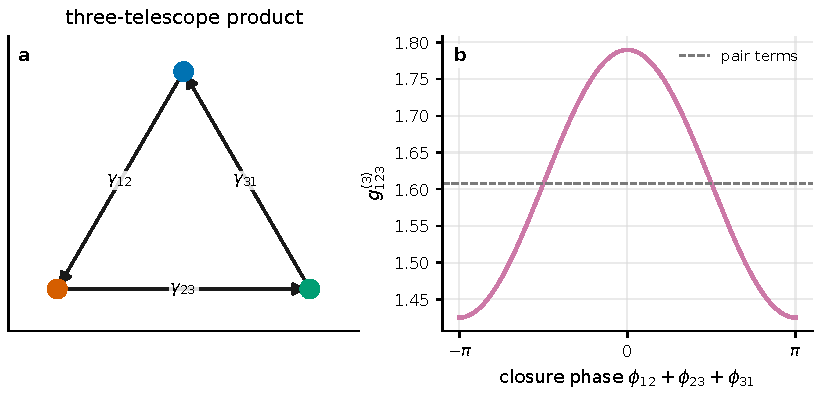
\includegraphics[width=0.92\linewidth]{figures/generated/chapter_04/ch04_g3_closure_phase.pdf}
\caption{三阶强度相关中闭合相位项的来源。左图中三台望远镜形成 \(\gamma_{12}\gamma_{23}\gamma_{31}\) 的闭合乘积；右图显示在固定 \(|\gamma_{ij}|\) 下，\(g^{(3)}\) 随闭合相位的余弦变化。二阶强度干涉只给 \(|\gamma|^2\)，三阶项才开始对相位组合敏感。}
\label{fig:e08-g3}
\end{figure}

\section{一扇门：把时间延迟换成空间基线}
\label{sec:e08-gateway}

本章从头到尾都在讲"时间延迟 \(\tau\)"——同一束光隔了 \(\tau\) 的呼应。最后一步，是把这套语言里的 \(\tau\) 换成\emph{空间基线} \(\bm B\)，一扇通往第 \ref{chap:e10} 章的门就打开了。

想象两台相隔 \(\bm B\) 的望远镜同时盯着同一颗恒星，各自记录强度涨落。把 \(g^{(1)}\) 的两个"时刻"换成两个"位置"，它就不再量"电场隔 \(\tau\) 记得多少相位"，而是量"相距 \(\bm B\) 的两点上电场有多相干"。而 van Cittert--Zernike 定理（第 \ref{chap:e10} 章会证）会告诉我们：这个空间版的 \(g^{(1)}(\bm B)\)，正是天空亮度分布的\textbf{复可见度}（complex visibility）——它是天体角结构的傅里叶分量。于是 Siegert 关系原样搬过来：

\[
  g^{(2)}(\bm B)-1=\zeta\,\big|g^{(1)}(\bm B)\big|^2
  =\zeta\,\big|V(\bm B)\big|^2 ,
\]

两台望远镜强度涨落的\emph{同步程度}，就直接给出复可见度的模平方 \(|V(\bm B)|^2\)。这就是 HBT 强度干涉的全部魔法：不必像振幅干涉那样把两台望远镜的电场用真空管道合束（那对光路稳定度的要求近乎苛刻），只靠事后比对两地各自记录的强度起伏，就能测到可见度模平方，进而反推恒星角直径。成立的前提，仍是本章反复强调的两条：源光近似高斯混沌光，且仪器归一化没把背景、模式数、时间响应混进 \(\zeta\)。

带着这扇门，我们就能走进第 \ref{chap:e10} 章——把"时间相关"升级成"空间相关"，把"相干时间"升级成"可见度曲线"，最终在第 \ref{chap:e11} 章从可见度反推出天体的像。

\section{本章要点}
\label{sec:e08-summary}

\begin{itemize}
  \item \textbf{两阶相干，两个朴素问题。}一阶 \(g^{(1)}(\tau)\)（式 \eqref{eq:e08-g1}）量电场的相位记忆：\(|g^{(1)}|\to1\) 相干、\(\to0\) 失忆，其衰减宽度就是相干时间 \(\tau_c\simeq1/\Delta\nu\)（780\,nm/1\,nm 给 \(\tau_c\approx2\,{\rm ps}\)）。二阶 \(g^{(2)}(\tau)\)（式 \eqref{eq:e08-g2-field}）量光子成对倾向。
  \item \textbf{三种统计三种峰。}泊松（相干态）\(g^{(2)}=1\)；热光聚束 \(g^{(2)}(0)=2\)；\(g^{(2)}(0)<1\) 反聚束，是非经典判据。经典写法 \(g^{(2)}=\langle II\rangle/\langle I\rangle^2\) 好用，但要警惕 \(I\) 是否已被响应卷积。
  \item \textbf{Siegert 关系是本章的桥。}\(g^{(2)}(\tau)=1+\zeta|g^{(1)}(\tau)|^2\)（式 \eqref{eq:e08-siegert}），来自高斯混沌光的四阶矩拆分（高斯矩/Wick 定理）：\(\langle II\rangle=\langle I\rangle^2+|G^{(1)}|^2\)。它让强度相关直接读出场相干模平方。谱形定峰形：矩形 sinc\(^2\)、洛伦兹指数、高斯高斯。\(\zeta\) 只收集模式、偏振、背景（有限时间响应另由卷积处理，不含在 \(\zeta\) 内）。\emph{对相干态不成立}。
  \item \textbf{望远镜里的稀释。}有限响应卷积守面积不守峰高，\(C_{\rm obs}\simeq C_{\rm true}(\tau_c/\Delta t_{\rm eff})(1/M)f_Af_B\)（式 \eqref{eq:e08-contrast}）。Guerin 实验：\(7800\,\text{\AA}\)、\(10\,\text{\AA}\)、\(\tau_c\approx2\,{\rm ps}\)、响应 \(\approx700\,{\rm ps}\)，观测峰只有 \(C_{\rm obs}\approx2\times10^{-3}\)。
  \item \textbf{估计量与噪声。}延迟直方图 \(\widehat g^{(2)}=H_{AB}/(r_Ar_B\,\delta\tau\,T)\)（式 \eqref{eq:e08-estimator}），误差 \(\sigma\sim N_{\rm pair}^{-1/2}\)（式 \eqref{eq:e08-shotnoise}）——一切靠数够事件对。
  \item \textbf{两扇门。}三阶 \(g^{(3)}\) 的闭合相位项通向第 \ref{chap:e11} 章的成像相位；把 \(\tau\) 换成基线 \(\bm B\)，\(g^{(1)}\) 就成了复可见度 \(V(\bm B)\)，通向第 \ref{chap:e10} 章的空间强度干涉。
\end{itemize}

\medskip
\noindent\textbf{想一想。}
\begin{enumerate}
  \item 把滤光片带宽从 \(10\,\text{\AA}\) 放宽到 \(100\,\text{\AA}\)，相干时间 \(\tau_c\) 怎么变？在响应 \(\Delta t_{\rm eff}\approx700\,{\rm ps}\) 不变的情况下，观测峰高 \(C_{\rm obs}\) 会升还是降，约变几倍？
  \item 有人测到某光源 \(g^{(1)}\) 在很长延迟内仍接近 1，却发现 \(g^{(2)}\equiv1\)。这更可能是热光还是激光？为什么它不违反 Siegert 关系？
  \item 若把两个通道的计数率各提高 10 倍、曝光时间加长 4 倍，单 bin 的随机符合数 \(N_{\rm pair}\) 变几倍？相应的统计误差 \(\sigma[\widehat g^{(2)}]\) 又变几倍？
\end{enumerate}


% ============================================================
\part{相干、干涉与成像}
\chapter{时间相干与一阶（振幅）干涉}
\label{chap:e09}

\begin{chapteropening}
到这里，我们已经知道光是一组模式的激发，其正频率场算符 \(\hat E^{(+)}\) 是第 \ref{chap:e05} 章引入的；而探测器只数强度、看不见电场的相位这件事，正是第 \ref{chap:e07} 章光电探测所讲的（一个光学周期只有几飞秒，任何探测器都太"慢"，只能把振荡抹平留下能量）。我们也知道一束光"记得自己相位"的时间只有相干时间 \(\tau_c\simeq1/\Delta\nu\) 那么长（第 \ref{chap:e02} 章）。可是既然相位看不见，我们凭什么谈论"相干"？答案是干涉：把一束光劈成两路、走不同的光程再合到一起，相位差就会在\emph{强度}上显形——亮纹、暗纹，一道一道的条纹。本章要做的，是把抽象的一阶相干度 \(g^{(1)}(\tau)\) 落到一台看得见摸得着的干涉仪上：推出条纹强度公式，定义条纹可见度（visibility），证明"可见度就是电场还记得多少相位"的直接读数；再顺着维纳--辛钦定理（Wiener--Khinchin theorem）搭一座桥，说明为什么"条纹随光程差变淡的快慢"竟能反过来告诉我们谱线的形状——这正是傅里叶变换光谱学的原理。最后我们把这套"时间延迟版"的相干推广到"两点空间版"，交到下一章 van Cittert--Zernike 定理与强度干涉的手上。
\end{chapteropening}

\section{从一条光路到两条光路}
\label{sec:e09-two-beams}

先把干涉仪画出来。最干净的例子是迈克尔逊干涉仪（Michelson interferometer）：一束光打到分束镜上，一半射向固定镜、一半射向可移动镜，两路各自原路返回、在分束镜后重新合并，一起落到同一个探测器上。两条光路的长度一般不等，差一个光程 \(\Delta\)（单位 cm）。杨氏双缝（Young's double slit）在几何上是它的兄弟：同一束光穿过两条缝，到达屏上某点时也走了不等的两段路，只不过那里的路程差来自\emph{空间}的两个取样点，本章末尾我们会回到这一点。现在先盯住迈克尔逊这种"同一束光、两段光程"的时间版本。

探测器面上的场，是两路场的叠加：
\[
  \hat E_{\rm det}(t)=\hat E_1(t)+\hat E_2(t),
\]
其中 \(\hat E_1\)、\(\hat E_2\) 是两路各自到达探测器的正频率场算符（第 \ref{chap:e05} 章）。探测器"太慢"，逐个光学周期的振荡它抹平了，留下的是在响应时间里平均的强度，正比于场模平方。于是这一点的平均强度是
\[
  I=\big\langle \hat E_{\rm det}^{(-)}(t)\,\hat E_{\rm det}^{(+)}(t)\big\rangle
   =\big\langle |\hat E_1+\hat E_2|^2\big\rangle .
\]
把模平方展开。这是最普通的代数 \(|a+b|^2=|a|^2+|b|^2+a^\ast b+ab^\ast\)，逐项取平均：
\[
  I=\underbrace{\big\langle|\hat E_1|^2\big\rangle}_{I_1}
   +\underbrace{\big\langle|\hat E_2|^2\big\rangle}_{I_2}
   +\big\langle \hat E_1^\ast \hat E_2\big\rangle
   +\big\langle \hat E_1 \hat E_2^\ast\big\rangle .
\]
前两项 \(I_1,I_2\) 是两路各自单独打开时的强度（若挡住另一路就只剩它）。后两项互为复共轭，两个复共轭相加等于二倍实部，所以
\begin{equation}
  I=I_1+I_2+2\,\mathrm{Re}\big\langle \hat E_1^\ast(t)\,\hat E_2(t)\big\rangle .
  \label{eq:e09-interference-raw}
\end{equation}
\begin{formulaexplain}
\(I_1,I_2\) 是两路各自的强度；最后那个交叉项 \(\langle\hat E_1^\ast\hat E_2\rangle\) 是"两路场彼此还记得多少"的相关。干涉的一切，全藏在这一项里。
\end{formulaexplain}

逐项交代。\(I_1,I_2\) 有强度量纲（CGS 下 \({\rm erg\,s^{-1}\,cm^{-2}}\) 量级，这里只用它们的相对大小）。真正携带信息的是交叉项 \(\langle\hat E_1^\ast(t)\hat E_2(t)\rangle\)：如果两路场毫无关系，这个平均等于零，探测器上就只有平淡的 \(I_1+I_2\)，没有条纹；如果两路场高度相关，交叉项很大，随光程差一扫就出现明暗对比强烈的条纹。所以\textbf{条纹的深浅，直接量的就是这条交叉相关}。

现在要把交叉项算清楚。关键的物理事实是：第 2 路只是第 1 路那束光被延迟、被搬动了一个光程 \(\Delta\) 而已——它们来自同一个源场，只是取自不同时刻。把归一化的复场记作 \(\varepsilon(t)\)（满足 \(\langle|\varepsilon|^2\rangle=1\)），两路可写成
\[
  \hat E_1(t)=\sqrt{I_1}\,\varepsilon(t),\qquad
  \hat E_2(t)=\sqrt{I_2}\,\varepsilon(t-\tau),\qquad
  \tau=\frac{\Delta}{c}.
\]
这里 \(\tau=\Delta/c\) 是光程差换算成的\emph{时间延迟}（单位 s），\(c\) 是光速。第 2 路的场，就是第 1 路的场倒退 \(\tau\) 时间取到的值。于是交叉项变成同一个场在相隔 \(\tau\) 的两个时刻的相关：
\[
  \big\langle \hat E_1^\ast(t)\,\hat E_2(t)\big\rangle
  =\sqrt{I_1 I_2}\,\big\langle \varepsilon^\ast(t)\,\varepsilon(t-\tau)\big\rangle .
\]
这里出现的是 \(\varepsilon(t-\tau)\)（第 2 路延迟了 \(\tau\)），而下面 \(g^{(1)}\) 的标准定义里写的是 \(\varepsilon(t+\tau)\)——两者相差一个复共轭，别急着划等号。用平稳性（相关只依赖延迟、不依赖绝对时刻）把时间原点平移 \(t\to t+\tau\)：
\[
  \big\langle \varepsilon^\ast(t)\,\varepsilon(t-\tau)\big\rangle
  =\big\langle \varepsilon^\ast(t+\tau)\,\varepsilon(t)\big\rangle
  =\big[g^{(1)}(\tau)\big]^\ast=g^{(1)}(-\tau) .
\]
好在最终代进式 \eqref{eq:e09-interference-raw} 的只是这一项的\emph{实部}、并会用到它的\emph{模}；而 \(|g^{(1)}|\) 是偶函数、实部对取复共轭又不变，所以把它直接换写成 \(g^{(1)}(\tau)\) 对条纹的模与实部\emph{毫无影响}。据此，它正是第 \ref{chap:e08} 章定义过的一阶相干度（first-order/amplitude coherence）。把归一化的一阶时间相干度记作
\begin{equation}
  g^{(1)}(\tau)=
  \frac{\big\langle \varepsilon^\ast(t)\,\varepsilon(t+\tau)\big\rangle}
       {\big\langle |\varepsilon(t)|^2\big\rangle},
  \qquad g^{(1)}(0)=1 ,
  \label{eq:e09-g1-def}
\end{equation}
\begin{formulaexplain}
\(g^{(1)}(\tau)\) 是同一束光相隔 \(\tau\) 的电场相关，除以自身强度归一化。它是复数：模 \(|g^{(1)}|\) 说"还记得多少"，幅角说"相位差了多少"。\(\tau=0\) 时场和自己完全相关，\(g^{(1)}(0)=1\)。
\end{formulaexplain}
其中 \(\tau\) 是时间延迟（单位 s），\(g^{(1)}\) 无量纲。它是复数：\(|g^{(1)}(\tau)|\) 从 1（\(\tau=0\)，完全相干）随延迟增大衰减到 0（相位记忆完全丢失）；它的幅角记录相位差。对平稳（stationary）光场，这个相关只依赖延迟 \(\tau\)，不依赖绝对时刻 \(t\)——这一点后面反复要用。

把交叉项代回式 \eqref{eq:e09-interference-raw}。这里要做一件对物理很关键的拆分。相干度 \(g^{(1)}(\tau)\) 的相位里其实混着两种快慢完全不同的东西：一种是载波相位（carrier phase），来自光程差在中心频率 \(\bar\nu\) 上累积的振荡；另一种是缓慢变化的残余相位。因为光程差每变化一个波长 \(\lambda\)，载波相位就转过整整 \(2\pi\)，而 \(|g^{(1)}|\) 几乎纹丝不动，所以把载波单独乘出来最自然。先定义载波相位
\[
  \delta=\frac{2\pi\Delta}{\lambda}=2\pi\bar\nu\,\tau ,
\]
再把这个载波从 \(g^{(1)}\) 里\emph{除掉}，得到一个只剩缓慢变化的复量，记作 \(\tilde g(\tau)\)（注意它是一个\emph{新符号}，不是 \(\arg g^{(1)}\) 本身）：
\[
  \tilde g(\tau)\equiv e^{+i2\pi\bar\nu\tau}\,g^{(1)}(\tau)
  =\big|g^{(1)}(\tau)\big|\,e^{\,i\varphi(\tau)} .
\]
乘上一个模为 1 的相位因子不改变模，所以 \(|\tilde g|=|g^{(1)}|\)；这里 \(\varphi(\tau)\) 就是\emph{去掉载波后剩下的缓慢残余相位}（无量纲，单位 rad），谱线对称时 \(\varphi\equiv0\)。把这条定义反解出 \(g^{(1)}\)：
\[
  g^{(1)}(\tau)=e^{-i2\pi\bar\nu\tau}\,\tilde g(\tau)
  =\big|g^{(1)}(\tau)\big|\,e^{\,i[\varphi(\tau)-\delta]} .
\]
于是取实部（\(\cos\) 是偶函数，\(\cos(\varphi-\delta)=\cos(\delta-\varphi)\)）得 \(\mathrm{Re}\,g^{(1)}=|g^{(1)}|\cos\!\big(\delta-\varphi(\tau)\big)\)，代回式 \eqref{eq:e09-interference-raw} 得到本节的中心结果——双光束干涉的条纹公式：
\begin{equation}
  I(\delta)=I_1+I_2+2\sqrt{I_1 I_2}\;\big|g^{(1)}(\tau)\big|\,
  \cos\!\big(\delta-\varphi(\tau)\big),
  \qquad \delta=\frac{2\pi\Delta}{\lambda},\ \ \tau=\frac{\Delta}{c}.
  \label{eq:e09-fringe}
\end{equation}
\begin{formulaexplain}
条纹强度 = 两路本底 \(I_1+I_2\) + 一个随光程差起伏的余弦项。余弦让明暗交替，它的\emph{振幅}正比于 \(|g^{(1)}(\tau)|\)——电场记得越多，条纹起伏越大。载波相位 \(\delta=2\pi\Delta/\lambda\) 是我们移动镜子扫的旋钮；\(\varphi(\tau)\) 是去掉载波后的缓慢残余相位，谱线对称时为零。
\end{formulaexplain}

把这条式子读透。\(\delta=2\pi\Delta/\lambda\) 是移动镜子直接控制的相位：镜子平移半个波长（光程差变一个波长），\(\delta\) 转过 \(2\pi\)，条纹走过明暗各一遍。所以随着我们扫描 \(\Delta\)，探测器读数在 \(I_{\max}\) 和 \(I_{\min}\) 之间来回摆——这就是条纹。摆动的幅度是 \(2\sqrt{I_1 I_2}\,|g^{(1)}(\tau)|\)：它有两个因子，\(2\sqrt{I_1I_2}\) 是两路光强搭配得好不好（等光强时最大），\(|g^{(1)}(\tau)|\) 是电场在延迟 \(\tau\) 后还记得多少相位。若 \(|g^{(1)}|=1\)，条纹在 \(I_1+I_2\) 上下满幅摆动；若 \(|g^{(1)}|=0\)，余弦项消失，探测器上一片均匀，没有条纹。换句话说：\textbf{条纹的存在与深浅，就是一阶相干的直接显影}。下一节我们把"深浅"这件事量化成一个标准数字。

\section{条纹可见度就是相干度的读数}
\label{sec:e09-visibility}

肉眼看条纹，第一印象是"清不清楚"——亮纹和暗纹反差大就清楚，反差小就模糊。把这个印象变成可测量的数字，就是条纹可见度（fringe visibility），由 Michelson 最早引入：
\begin{equation}
  \mathcal V=\frac{I_{\max}-I_{\min}}{I_{\max}+I_{\min}} .
  \label{eq:e09-visibility-def}
\end{equation}
\begin{formulaexplain}
\(\mathcal V\) 用最亮纹 \(I_{\max}\) 和最暗纹 \(I_{\min}\) 的反差除以它们的和。全黑到全亮时 \(\mathcal V=1\)，一片灰没有条纹时 \(\mathcal V=0\)。它是"条纹有多清楚"的标准刻度。
\end{formulaexplain}
\(I_{\max}\)、\(I_{\min}\) 分别是扫描 \(\delta\) 时探测器读到的最大、最小强度，\(\mathcal V\) 无量纲，介于 0 和 1 之间。为什么用这个组合而不用别的？因为它\emph{自动约掉总亮度}：把光源调亮一倍，\(I_{\max},I_{\min}\) 同时翻倍，比值不变。可见度只关心"反差"，不关心"多亮"，正好对应我们想问的"相干性"。

现在把式 \eqref{eq:e09-fringe} 代进去算。扫描 \(\delta\) 时，余弦在 \(+1\) 和 \(-1\) 之间取值（残余相位 \(\varphi(\tau)\) 变化很慢，在一条条纹的尺度上可当常数，只是给条纹整体平移一点，不改变峰谷高度）：
\[
  I_{\max}=I_1+I_2+2\sqrt{I_1 I_2}\,|g^{(1)}(\tau)|
  \quad(\cos=+1),
\]
\[
  I_{\min}=I_1+I_2-2\sqrt{I_1 I_2}\,|g^{(1)}(\tau)|
  \quad(\cos=-1).
\]
两式相减，本底 \(I_1+I_2\) 抵消，余下两倍的余弦振幅：
\[
  I_{\max}-I_{\min}=4\sqrt{I_1 I_2}\,|g^{(1)}(\tau)| .
\]
两式相加，余弦振幅抵消，余下两倍本底：
\[
  I_{\max}+I_{\min}=2\,(I_1+I_2).
\]
相除，那个公共的 2 约掉，得到可见度与相干度的桥梁：
\begin{equation}
  \mathcal V(\tau)=\frac{2\sqrt{I_1 I_2}}{I_1+I_2}\,\big|g^{(1)}(\tau)\big| .
  \label{eq:e09-visibility-g1}
\end{equation}
\begin{formulaexplain}
可见度 = 光强搭配因子 \(2\sqrt{I_1I_2}/(I_1+I_2)\) 乘以相干度模 \(|g^{(1)}(\tau)|\)。前者只和两路亮度比有关，后者才是光本身的相干性。等光强时前者为 1，可见度\emph{就是} \(|g^{(1)}|\)。
\end{formulaexplain}

这条式子把两件事干净地分开了。第一个因子 \(2\sqrt{I_1 I_2}/(I_1+I_2)\) 纯粹是几何搭配：它是两路光强的几何平均比算术平均，永远 \(\le 1\)，只有当 \(I_1=I_2\) 时才等于 1（这是均值不等式，几何平均等于算术平均当且仅当两数相等）。它衡量的是"仪器有没有把两路调成等亮"，和光的相干性无关。第二个因子 \(|g^{(1)}(\tau)|\) 才是物理主角。于是在实验里人们总是刻意把两路调成等光强 \(I_1=I_2\)，此时搭配因子为 1，可见度和相干度直接相等：
\begin{equation}
  \boxed{\;\mathcal V(\tau)=\big|g^{(1)}(\tau)\big|\quad(I_1=I_2)\;}
  \label{eq:e09-visibility-equals-g1}
\end{equation}
\begin{formulaexplain}
等光强时，你在干涉图上量到的条纹清晰度 \(\mathcal V\)，\emph{就是}那个抽象的一阶相干度的模 \(|g^{(1)}(\tau)|\)。抽象的"电场还记得相位"变成了看得见的条纹对比度。
\end{formulaexplain}

这就是本章想让你记住的第一句话：\textbf{条纹可见度是"电场还记得相位"的直接读数}。第 \ref{chap:e08} 章里 \(g^{(1)}\) 是一个写在算符平均里的抽象对象，你没法直接"看到"它；现在它有了肉眼可读的化身——把干涉仪的延迟调到 \(\tau\)，数一数亮纹暗纹的反差，得到的就是 \(|g^{(1)}(\tau)|\)。相位那件探测器"看不见"的东西，通过干涉在强度上留下了它的影子，而可见度就是这道影子的深浅。

顺带一提，等光强双缝的两种极端很好记：\(\mathcal V=1\) 表示完全相干，条纹从全黑到全亮，天文上对应"这条基线还完全没分辨开源"；\(\mathcal V=0\) 表示完全不相干，屏上只有两缝各自照明的平坦叠加，没有条纹，对应"源在这个尺度上已被彻底分辨、相干性洗光"。真实观测几乎都落在两者之间，可见度是个介于 0 和 1 的小数，它的具体数值携带着我们想要的信息。

\section{相干长度与相干时间}
\label{sec:e09-coherence-length}

式 \eqref{eq:e09-visibility-equals-g1} 说可见度随延迟 \(\tau\) 变化。那它怎么变？物理直觉很清楚：延迟越大，第 2 路取自越久以前的场，而光"记得自己相位"的时间只有相干时间 \(\tau_c\simeq1/\Delta\nu\)（第 \ref{chap:e02} 章）那么长；一旦延迟超过 \(\tau_c\)，两路的相位早已各走各的、失去关联，\(|g^{(1)}|\to0\)，条纹随之消失。所以：

\begin{quote}
\textbf{条纹随光程差增大而变淡，衰减的特征尺度就是相干长度。}
\end{quote}

把相干时间换算成光走过的距离，就是相干长度（coherence length）：
\begin{equation}
  \ell_c=c\,\tau_c\simeq\frac{c}{\Delta\nu}\simeq\frac{\lambda^2}{\Delta\lambda},
  \qquad
  \Delta\nu\simeq\frac{c\,\Delta\lambda}{\lambda^2}.
  \label{eq:e09-coherence-length}
\end{equation}
\begin{formulaexplain}
\(\ell_c\) 是"两路光程差还能看到条纹"的最大尺度（单位 cm）。它等于相干时间 \(\tau_c\) 乘光速。带宽 \(\Delta\nu\) 越宽（或 \(\Delta\lambda\) 越大），相干长度越短，条纹越早消失。
\end{formulaexplain}
逐项交代。\(\ell_c\) 单位是 cm（或 m）；\(\tau_c\) 是相干时间（s）；\(\Delta\nu\) 是频率带宽（Hz）；\(\lambda\) 是中心波长，\(\Delta\lambda\) 是波长带宽。最后一步的带宽换算 \(\Delta\nu\simeq c\,\Delta\lambda/\lambda^2\) 来自对 \(\nu=c/\lambda\) 求微分（\(|{\rm d}\nu|=(c/\lambda^2)|{\rm d}\lambda|\)），与第 \ref{chap:e02} 章一致。物理含义一句话：\emph{当两路光程差超过 \(\ell_c\)，条纹就基本看不见了}。它是干涉仪"能容忍多大光程失配"的硬指标。

代入真实数字，感受这个尺度跨了多少量级。

\paragraph{白光。}肉眼所见的白光带宽极宽，取 \(\lambda\simeq550\,{\rm nm}\)、\(\Delta\lambda\simeq300\,{\rm nm}\)（整个可见光）：
\[
  \Delta\nu\simeq\frac{(3\times10^{10}\,{\rm cm\,s^{-1}})(3\times10^{-5}\,{\rm cm})}
  {(5.5\times10^{-5}\,{\rm cm})^2}\simeq3\times10^{14}\,{\rm Hz},
  \quad
  \tau_c\simeq3.4\times10^{-15}\,{\rm s},
  \quad
  \ell_c\simeq1\,\mu{\rm m}.
\]
白光的相干长度只有大约一微米——两三个波长！这正是为什么用白光看迈克尔逊干涉时，只有两臂几乎完全等长的一小段范围内能看到彩色条纹，稍微一移就糊掉。它也解释了肥皂膜、油膜上的彩色干涉为什么只在膜很薄时出现。

\paragraph{窄带滤光片。}加一片 \(\Delta\lambda=1\,{\rm nm}\) 的滤光片，中心 \(\lambda=550\,{\rm nm}\)：\(\Delta\nu\simeq1\times10^{12}\,{\rm Hz}\)，\(\tau_c\simeq1\,{\rm ps}\)，\(\ell_c\simeq0.3\,{\rm mm}\)。相干长度一下涨到亚毫米——现在两臂允许差上零点几毫米还看得见条纹。Guerin 等人的恒星聚束实验用的正是这个量级：\(\lambda\simeq780\,{\rm nm}\)、\(\Delta\lambda=1\,{\rm nm}\) 给出 \(\tau_c\simeq2\,{\rm ps}\)、\(\ell_c\simeq0.6\,{\rm mm}\) \citep{2017MNRAS.472.4126G}。

\paragraph{激光。}一台单频激光器带宽可窄到 \(\Delta\nu=1\,{\rm MHz}\)：\(\tau_c=1\,\mu{\rm s}\)，\(\ell_c=c\tau_c=300\,{\rm m}\)。相干长度几百米——这就是为什么激光能做长臂干涉（乃至引力波探测器那样公里级的臂长）而白光绝无可能。把带宽再压到 kHz，相干长度进入几百公里。

一张表把跨越十几个数量级的图景收进眼底：从白光的微米，到窄带的亚毫米，到激光的百米，相干长度完全由带宽决定。记住这条链子，它在后面每一次谈"能容忍多大延迟/光程差"时都会回来。

\section{维纳--辛钦桥：条纹衰减反推谱线}
\label{sec:e09-wiener-khinchin}

前一节说 \(|g^{(1)}(\tau)|\) 随 \(\tau\) 在相干时间尺度上衰减，但没说\emph{按什么形状}衰减——是先慢后快，还是指数下滑，还是振荡着掉下去？这个形状不是随便的，它由光的\textbf{谱线形状}唯一决定。把这层关系讲清楚的，是维纳--辛钦定理：\(g^{(1)}(\tau)\) 与归一化功率谱互为傅里叶变换。这座桥有个惊人的推论——\emph{测条纹随延迟怎么衰减，就能反推出谱线长什么样}，这正是傅里叶变换光谱学（Fourier-transform spectroscopy）的原理。第 \ref{chap:e02} 章预告过它，这里把它自足地建立起来。

推导只需一个物理输入：平稳光场的不同频率分量互不相关。先把复场按频率展开（这是第 \ref{chap:e02} 章的傅里叶分析，只保留正频率部分，对应第 \ref{chap:e05} 章的 \(\hat E^{(+)}\)）：
\[
  \varepsilon(t)=\int_0^\infty \tilde\varepsilon(\nu)\,e^{-i2\pi\nu t}\,{\rm d}\nu,
  \qquad
  \varepsilon^\ast(t)=\int_0^\infty \tilde\varepsilon^\ast(\nu')\,e^{+i2\pi\nu' t}\,{\rm d}\nu' .
\]
其中 \(\tilde\varepsilon(\nu)\) 是频率 \(\nu\) 处的复振幅。把两者相乘、对延迟 \(\tau\) 写出一阶相关 \(G^{(1)}(\tau)=\langle\varepsilon^\ast(t)\varepsilon(t+\tau)\rangle\)：
\[
  G^{(1)}(\tau)
  =\int_0^\infty\!\!\int_0^\infty
  \big\langle \tilde\varepsilon^\ast(\nu')\,\tilde\varepsilon(\nu)\big\rangle\,
  e^{+i2\pi\nu' t}\,e^{-i2\pi\nu(t+\tau)}\,{\rm d}\nu\,{\rm d}\nu' .
\]
现在用上那个唯一的物理输入。光场\emph{平稳}——统计性质不随时间原点改变——数学上强制不同频率分量互不相关，只有同一频率才有非零关联。这是一个标准结果（平稳过程的谱表示定理，可当作已知）：
\[
  \big\langle \tilde\varepsilon^\ast(\nu')\,\tilde\varepsilon(\nu)\big\rangle
  =S(\nu)\,\delta(\nu-\nu') ,
\]
其中 \(S(\nu)\ge0\) 就是功率谱密度（power spectral density，即谱线形状），\(\delta\) 是狄拉克函数。之所以必须这样，是因为若 \(\nu\ne\nu'\) 的关联不为零，上式里就会残留 \(e^{i2\pi(\nu'-\nu)t}\) 这种含 \(t\) 的因子，破坏"结果只依赖 \(\tau\) 不依赖 \(t\)"的平稳性。代入后 \(\delta(\nu-\nu')\) 把一重积分吃掉（令 \(\nu'=\nu\)），含 \(t\) 的指数 \(e^{+i2\pi\nu t}e^{-i2\pi\nu t}=1\) 恰好抵消：
\[
  G^{(1)}(\tau)=\int_0^\infty S(\nu)\,e^{-i2\pi\nu\tau}\,{\rm d}\nu .
\]
最后除以 \(\tau=0\) 时的值 \(G^{(1)}(0)=\int S(\nu)\,{\rm d}\nu\)（总功率）归一化，得到维纳--辛钦定理：
\begin{equation}
  g^{(1)}(\tau)=
  \frac{\displaystyle\int_0^\infty S(\nu)\,e^{-i2\pi\nu\tau}\,{\rm d}\nu}
       {\displaystyle\int_0^\infty S(\nu)\,{\rm d}\nu} .
  \label{eq:e09-wiener-khinchin}
\end{equation}
\begin{formulaexplain}
一阶相干度 \(g^{(1)}(\tau)\) 是归一化功率谱 \(S(\nu)\) 的傅里叶变换。谱线越宽，\(g^{(1)}\) 衰减越快（相干时间越短）；谱线的具体形状，决定条纹包络的具体形状。
\end{formulaexplain}
\(S(\nu)\) 是功率谱密度（谱线形状），\(\nu\) 单位 Hz；分母把总功率归一化，保证 \(g^{(1)}(0)=1\)。这条式子把"时域的相干"和"频域的谱线"锁成一对傅里叶变换。它立刻给出前一节相干时间的来历：谱线越宽（\(\Delta\nu\) 越大），它的傅里叶变换越窄（\(\tau_c\simeq1/\Delta\nu\) 越小），条纹越早消失。下面两个例子把"谱线形状 → 条纹衰减形状"的对应具体算出来，用的都是标准傅里叶变换对。

\paragraph{例一：矩形谱 → sinc 衰减。}设谱线是一段宽度为 \(\Delta\nu\)、中心在 \(\bar\nu\) 的矩形（理想的平顶窄带滤光片），归一化后 \(S(\nu)=1/\Delta\nu\)（在带内），代入式 \eqref{eq:e09-wiener-khinchin}。令 \(\nu=\bar\nu+f\)，\(f\in[-\Delta\nu/2,\,\Delta\nu/2]\)：
\[
  g^{(1)}(\tau)=\frac{1}{\Delta\nu}\int_{-\Delta\nu/2}^{\Delta\nu/2}
  e^{-i2\pi(\bar\nu+f)\tau}\,{\rm d}f
  =\frac{e^{-i2\pi\bar\nu\tau}}{\Delta\nu}
  \int_{-\Delta\nu/2}^{\Delta\nu/2}e^{-i2\pi f\tau}\,{\rm d}f .
\]
里面是最基本的指数积分 \(\int e^{-i2\pi f\tau}{\rm d}f=e^{-i2\pi f\tau}/(-i2\pi\tau)\)，代上下限并用 \(e^{-ix}-e^{+ix}=-2i\sin x\)：
\[
  \int_{-\Delta\nu/2}^{\Delta\nu/2}e^{-i2\pi f\tau}\,{\rm d}f
  =\frac{e^{-i\pi\Delta\nu\tau}-e^{+i\pi\Delta\nu\tau}}{-i2\pi\tau}
  =\frac{-2i\sin(\pi\Delta\nu\tau)}{-i2\pi\tau}
  =\frac{\sin(\pi\Delta\nu\tau)}{\pi\tau} .
\]
除以 \(\Delta\nu\)，凑成标准的 sinc 函数 \({\rm sinc}(x)\equiv\sin(\pi x)/(\pi x)\)：
\begin{equation}
  g^{(1)}(\tau)=e^{-i2\pi\bar\nu\tau}\,\frac{\sin(\pi\Delta\nu\tau)}{\pi\Delta\nu\tau}
  =e^{-i2\pi\bar\nu\tau}\,{\rm sinc}(\Delta\nu\,\tau),
  \qquad
  \big|g^{(1)}(\tau)\big|=\big|{\rm sinc}(\Delta\nu\,\tau)\big| .
  \label{eq:e09-rect-sinc}
\end{equation}
\begin{formulaexplain}
矩形谱给出 sinc 型可见度：条纹随延迟先按 sinc 衰减，在 \(\tau=1/\Delta\nu\) 处第一次归零，之后还有一串越来越矮的旁瓣。第一零点位置就标出了带宽。
\end{formulaexplain}
可见度 \(\mathcal V=|g^{(1)}|=|{\rm sinc}(\Delta\nu\tau)|\) 在 \(\tau=1/\Delta\nu=\tau_c\) 处第一次掉到零，此后还有一串越来越矮的旁瓣（sinc 的次峰）。因子 \(e^{-i2\pi\bar\nu\tau}\) 就是那个快速载波：\(2\pi\bar\nu\tau=2\pi\Delta/\lambda=\delta\)，正是式 \eqref{eq:e09-fringe} 里被我们单独乘出来当旋钮扫的载波相位（即 \(e^{-i2\pi\bar\nu\tau}=e^{-i\delta}\)）。此时去掉载波后的复量 \(\tilde g(\tau)=e^{+i2\pi\bar\nu\tau}g^{(1)}(\tau)={\rm sinc}(\Delta\nu\tau)\) 是\emph{实数}，故残余相位 \(\varphi(\tau)\equiv0\)（矩形谱对称）——与第 \ref{sec:e09-two-beams} 节那次拆分严丝合缝对上。注意 \(|g^{(1)}|^2={\rm sinc}^2(\Delta\nu\tau)\) 恰好是第 \ref{chap:e08} 章 Siegert 关系里出现的那条二阶聚束峰形状——两章在此对上了。

\paragraph{例二：洛伦兹谱 → 指数衰减。}许多谱线（碰撞展宽、自然线宽、单模腔泄漏）是洛伦兹形（Lorentzian）：\(S(\nu)\propto 1/[(\nu-\bar\nu)^2+(\Delta\nu/2)^2]\)，其中 \(\Delta\nu\) 是半高全宽（FWHM）。洛伦兹函数的傅里叶变换是一个双边衰减指数——这是标准傅里叶变换对（洛伦兹 \(\leftrightarrow\) 指数），直接引用：
\begin{equation}
  g^{(1)}(\tau)=e^{-i2\pi\bar\nu\tau}\,e^{-\pi\Delta\nu\,|\tau|}
  =e^{-i2\pi\bar\nu\tau}\,e^{-|\tau|/\tau_c},
  \qquad
  \tau_c=\frac{1}{\pi\Delta\nu} .
  \label{eq:e09-lorentz-exp}
\end{equation}
\begin{formulaexplain}
洛伦兹谱给出纯指数衰减的可见度 \(|g^{(1)}|=e^{-|\tau|/\tau_c}\)，没有零点、没有旁瓣，一路平滑下滑。衰减常数 \(\tau_c=1/(\pi\Delta\nu)\) 直接给出线宽。
\end{formulaexplain}
现在 \(|g^{(1)}(\tau)|=e^{-|\tau|/\tau_c}\) 是平滑的指数衰减，没有零点也没有旁瓣，和矩形谱的振荡形成鲜明对照。它对应第 \ref{chap:e08} 章里 Siegert 关系给出的指数型二阶相关峰。测到条纹随延迟做纯指数衰减，就等于测到谱线是洛伦兹形，衰减常数 \(\tau_c\) 反过来给出线宽 \(\Delta\nu=1/(\pi\tau_c)\)。

这就是傅里叶变换光谱学的全部逻辑：不去用棱镜或光栅把频率一根根排开，而是\emph{扫描干涉仪的延迟}，记录可见度 \(\mathcal V(\tau)=|g^{(1)}(\tau)|\)（连同相位），再对这条曲线做一次傅里叶反变换，谱线 \(S(\nu)\) 就还原出来了。它的威力在于分辨率由\emph{最大延迟}决定：能扫到的延迟越大，频率分辨越细。对天文上那些普通光谱仪难以企及的极窄谱线（如 \(\eta\) Car 附近的天体激光候选线，需要 \(R\sim10^8\) 的分辨率），用相干性随延迟的衰减来反推线宽，往往是唯一可行的路子。图 \ref{fig:e09-fourier-visibility} 用几种源结构展示了这种"结构 \(\leftrightarrow\) 可见度"的傅里叶对应——虽然画的是空间版本（下一节的主题），但傅里叶的骨架和这里时间版本完全同构。

\section{两条路线：振幅干涉与强度干涉}
\label{sec:e09-two-routes}

到此我们讲的都是振幅干涉（amplitude interferometry）：把两路光的\emph{电场}在光学上真正合到一起，让它们相加、干涉，从条纹里读复可见度 \(\mathcal V\,e^{i\varphi(\tau)}\)（\(\varphi\) 是扣掉已知载波 \(\delta\) 后的残余相位）。它的最大优点是\textbf{相位也测得到}——条纹峰相对载波的位置就直接给出 \(\varphi(\tau)\)，这在成像时至关重要。但它有一个苛刻的代价：既然干涉发生在电场层面，两路光程必须稳定到\emph{波长的零头}。可见光波长半微米，光程漂移哪怕几十纳米，条纹就糊了。大气的活塞相位（piston，整束光被湍流随机推前推后的光程抖动）在光学波段是致命的，它让长基线振幅干涉极其难做。

第 \ref{chap:e10} 章的强度干涉（intensity interferometry，即 Hanbury Brown--Twiss）走的是另一条路：\emph{不在光学上合束}，两路光各自独立探测，事后比较两路\emph{强度涨落}是否同步。由 Siegert 关系（第 \ref{chap:e08} 章）\(g^{(2)}-1\propto|g^{(1)}|^2\)，它测到的是可见度的\emph{模平方} \(|\mathcal V|^2\)，丢掉了相位。代价换来一个巨大的好处：因为比较的是探测\emph{之后}的电信号涨落，需要稳定的不再是光程，而是\emph{电子对齐}——只要把两路电信号对齐到\emph{探测器响应时间的零头}即可。1\,GHz 电子带宽对应约 30\,cm 的容差，光程差几厘米也无所谓；大气 piston 在纳秒级强度相关面前几乎不是噪声源。这就是为什么光学质量远不及专用干涉仪的切伦科夫望远镜（Cherenkov telescope，为纳秒闪光设计、口径大、探测器快）反而能拿来做强度干涉 \citep{2020NatAs...4.1164A}。

把这两条路线并排列清楚，是理解第 \ref{chap:e10} 章的关键：

\begin{longtable}{p{0.24\linewidth}p{0.34\linewidth}p{0.34\linewidth}}
\toprule
对照项 & 一阶（振幅）干涉 & 二阶（强度）干涉 \\
\midrule
合束方式 & 电场在光学上真正合并、相加 & 各自独立探测，事后比较强度涨落 \\
直接测到的量 & 复可见度 \(\mathcal V\,e^{i\varphi}\)（含相位） & \(|\mathcal V|^2=|g^{(1)}|^2\)（丢相位） \\
所依赖的相干 & 一阶相干 \(g^{(1)}\) & 二阶相干 \(g^{(2)}\)，经 Siegert 联回 \(|g^{(1)}|^2\) \\
稳定性要求 & 光程需稳到波长的零头（\(\sim\)nm） & 电子对齐到响应时间的零头（\(\sim\)ns/cm） \\
大气 piston & 极敏感，长基线很难 & 几乎不敏感 \\
信噪与光子 & 相对高效，但对光程、湍流苛刻 & 信号浅（\(\sim10^{-6}\)），靠海量光子对累积 \\
相位/成像 & 直接给相位，利于成像 & 需三阶相关或相位恢复才补回相位 \\
典型系统 & Michelson 恒星干涉仪、CHARA、VLTI & Narrabri、VERITAS、MAGIC \\
\bottomrule
\end{longtable}

一句话概括这张表：\textbf{振幅干涉用光程的稳定换来了相位，强度干涉用相位的丢失换来了对光程的宽容}。两者不是谁取代谁，而是各自适配不同的波段、基线和目标。下一章我们主攻强度干涉这条路线，但它测到的 \(|g^{(1)}|^2\) 里的 \(g^{(1)}\)，就是本章一手建立的一阶相干——只不过从"时间延迟版"换成了"两点空间版"。

\section{从时间延迟到两点空间}
\label{sec:e09-spatial-gamma}

本章从头到尾的 \(g^{(1)}(\tau)\)，比较的是\emph{同一点}上相隔时间 \(\tau\) 的两份场。现在把镜头一转：如果比较的不是"同一点的两个时刻"，而是"同一时刻的两个地点"呢？这正是杨氏双缝在做的事——两条缝是空间里的两个取样点，屏上的条纹检验的是这两点的场是否相干。把时间延迟 \(\tau\) 换成两台望远镜之间的空间基线，一阶相干就从 \(g^{(1)}(\tau)\) 升级成两点空间相干度 \(\gamma_{12}\)：
\begin{equation}
  \gamma_{12}=
  \frac{\big\langle \hat E_1^\ast(t)\,\hat E_2(t)\big\rangle}
       {\sqrt{\big\langle|\hat E_1(t)|^2\big\rangle\,\big\langle|\hat E_2(t)|^2\big\rangle}} ,
  \label{eq:e09-gamma12}
\end{equation}
\begin{formulaexplain}
\(\hat E_1,\hat E_2\) 是两台望远镜\emph{同一时刻}接收到的场；分子是跨望远镜的场相关，分母用各自强度归一化。\(\gamma_{12}\) 是复相干度：模给相干强弱（即可见度），幅角给傅里叶相位。
\end{formulaexplain}
这里 \(\hat E_1,\hat E_2\) 是相隔一条基线 \(\bm B\) 的两台望远镜同时接收的场，\(\gamma_{12}\) 无量纲、是复数。它和本章的 \(g^{(1)}(\tau)\) 是同一个数学对象的两个化身：一个沿时间轴、一个沿空间基线。等光强双缝的可见度 \(\mathcal V=|\gamma_{12}|\)（式 \eqref{eq:e09-visibility-equals-g1} 的空间版），条纹峰的位置给出 \(\arg\gamma_{12}\)。

\begin{figure}[tbp]
\centering
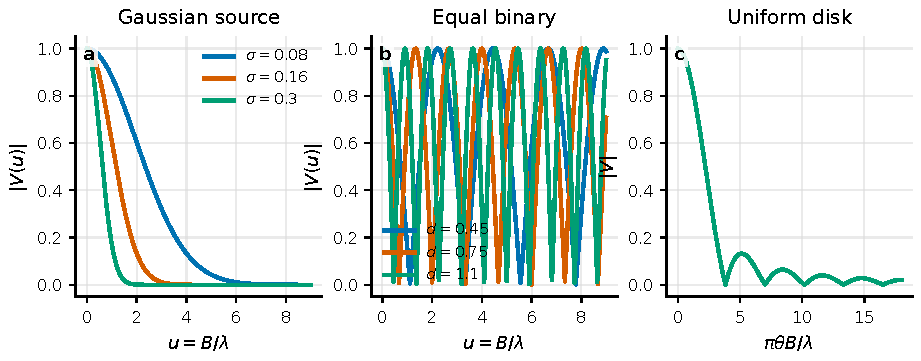
\includegraphics[width=0.9\linewidth]{figures/generated/chapter_01/ch01_fourier_visibility.pdf}
\caption{几种天空亮度结构给出的归一化可见度 \(|V|\) 随空间频率的变化：高斯源平滑下降，等亮双星产生余弦振荡，均匀圆盘因边缘锐利而出现零点和旁瓣。这与本章时间版的"谱线形状 \(\leftrightarrow\) 条纹衰减"完全同构——矩形谱的 sinc 旁瓣，对应均匀圆盘的 Bessel 旁瓣；只是把"频率谱"换成了"天空亮度分布"，"时间延迟"换成了"空间基线"。}
\label{fig:e09-fourier-visibility}
\end{figure}

这一步换轴，威力惊人。维纳--辛钦定理说"\(g^{(1)}(\tau)\) 是功率谱 \(S(\nu)\) 的傅里叶变换"；它的空间孪生兄弟——下一章的主角 van Cittert--Zernike 定理——将说"\(\gamma_{12}\) 是天空亮度分布 \(I(l,m)\) 的傅里叶变换"。于是本章每一条结论都有一个空间对应：条纹衰减的形状告诉我们谱线形状，正如可见度随基线的形状告诉我们\emph{源的角结构}；矩形谱的 sinc 旁瓣，对应均匀圆盘的 Bessel 旁瓣（图 \ref{fig:e09-fourier-visibility}）；相干长度 \(\ell_c\) 之于延迟，正如某个临界基线之于角尺度。把这套时间相干的直觉整体平移到空间，就是我们迈进空间相干与成像的门票。

带着一句话过渡到下一章：\textbf{可见度是一阶相干的读数，而一阶相干沿时间轴给出谱线、沿空间基线给出图像}。第 \ref{chap:e10} 章就从 \(\gamma_{12}\) 出发，用 van Cittert--Zernike 定理把它变成天空的傅里叶分量，再用强度干涉把 \(|\gamma_{12}|^2\) 测出来，一步步走向恒星角直径和成像。

\section{本章要点}
\label{sec:e09-summary}

\begin{itemize}
  \item \textbf{条纹公式。}两路光程差 \(\Delta\) 引入载波相位 \(\delta=2\pi\Delta/\lambda\) 与时间延迟 \(\tau=\Delta/c\)，探测强度 \(I(\delta)=I_1+I_2+2\sqrt{I_1I_2}\,|g^{(1)}(\tau)|\cos(\delta-\varphi(\tau))\)，其中 \(\varphi(\tau)\) 是去掉载波后的缓慢残余相位（谱线对称时为零）。余弦项的振幅正比于一阶相干度 \(|g^{(1)}|\)。
  \item \textbf{可见度就是相干度的读数。}\(\mathcal V=(I_{\max}-I_{\min})/(I_{\max}+I_{\min})=\dfrac{2\sqrt{I_1I_2}}{I_1+I_2}|g^{(1)}(\tau)|\)；等光强时 \(\mathcal V=|g^{(1)}(\tau)|\)。抽象的"电场还记得相位"变成了肉眼可读的条纹对比度。
  \item \textbf{相干长度。}条纹随光程差增大而变淡，特征尺度是 \(\ell_c=c\tau_c\simeq\lambda^2/\Delta\lambda\)：白光约 1\,\(\mu\)m，1\,nm 窄带约 0.3\,mm，MHz 激光约 300\,m。
  \item \textbf{维纳--辛钦桥。}\(g^{(1)}(\tau)\) 是归一化功率谱的傅里叶变换；矩形谱给 \(|g^{(1)}|=|{\rm sinc}(\Delta\nu\tau)|\)（有零点、有旁瓣），洛伦兹谱给 \(|g^{(1)}|=e^{-|\tau|/\tau_c}\)（纯指数）。因此测条纹随延迟的衰减能反推谱线形状——傅里叶变换光谱学的原理。
  \item \textbf{两条路线。}振幅干涉直接测复可见度（含相位）但要求光程稳到波长零头、对大气 piston 敏感；强度干涉只测 \(|\mathcal V|^2\)、丢相位，但只需电子对齐到响应时间零头（见对照表，引出第 \ref{chap:e10} 章）。
  \item \textbf{换轴到空间。}把时间延迟版的 \(g^{(1)}(\tau)\) 换成两点空间版的 \(\gamma_{12}\)，可见度 \(\mathcal V=|\gamma_{12}|\)；它是下一章 van Cittert--Zernike 定理与强度干涉的主角。
\end{itemize}

\medskip
\noindent\textbf{想一想。}
\begin{enumerate}
  \item 一台迈克尔逊干涉仪在白光下只有两臂几乎等长时才见到彩色条纹；换成 \(\Delta\lambda=1\,{\rm nm}\) 的窄带滤光片后，允许的两臂光程差扩大到多少？用式 \eqref{eq:e09-coherence-length} 估一估。
  \item 两路光强比为 \(I_1:I_2=4:1\)，即使光完全相干（\(|g^{(1)}|=1\)），条纹可见度最高能到多少？这说明"看不到满幅条纹"未必意味着不相干。
  \item 若测得可见度随延迟做纯指数衰减 \(\mathcal V(\tau)=e^{-|\tau|/\tau_c}\)，\(\tau_c=1\,{\rm ns}\)，对应的谱线是什么形状、线宽 \(\Delta\nu\) 是多少？换算成波长这条线有多"窄"？
\end{enumerate}

\chapter{空间相干、van Cittert--Zernike 与强度干涉}
\label{chap:e10}

\begin{chapteropening}
第 \ref{chap:e09} 章讲的是"时间版"的相干：同一束光，此刻和稍后一会儿，还记不记得自己的相位。这一章把同样的问题搬到空间里去问。想象两台望远镜，相隔几十米、几百米，甚至几公里，同时盯着夜空里同一颗星。它们各自接到的光，是不是"同一个波前上的两小块"？如果是，两路强度会一起明、一起暗，涨落同步；如果这颗星在天上张开的角度大到一定程度，两台望远镜采到的就是波前上已经"错开"的两块，涨落各走各的，不再同步。神奇的是，同步程度的高低，直接告诉我们这颗星有多大——哪怕它在最大的光学望远镜里也只是一个点。本章要把这条链子一环一环接起来：先用纯几何算出"两台望远镜看到多细的角结构"，再用 van Cittert--Zernike 定理把"天空的样子"翻译成"相干度"，然后借第 \ref{chap:e08} 章的 Siegert 关系，说明为什么\emph{不用把两束光合到一起、只比较各自强度的抖动}就能测出恒星的大小。最后我们会碰到强度干涉的软肋——相位丢了——以及它作为交换换来的好处：几乎不怕大气抖动。
\end{chapteropening}

\section{几何：两台望远镜、一条基线、一个角尺度}
\label{sec:e10-geometry}

先把相关器、光子、量子统计统统放一边，只看一件几何事实——这件事连相机都用不上，一根尺子和一点三角就够了。

来自天空某个方向的星光，在离我们足够远的地方，波前已经拉平成一张几乎笔直的平面（这就是"远场"）。设这颗星在天上的方向由单位矢量 \(\bm s\) 指定。两台望远镜分别站在位置 \(\bm x_1\) 和 \(\bm x_2\)，它们之间的连线矢量叫\textbf{基线}（baseline）：
\[
  \bm B=\bm x_2-\bm x_1 .
\]
同一张平面波前先扫过一台望远镜，再扫过另一台，走的路程不一样。这段\textbf{程差}（path difference）等于把基线投影到星光传播方向上的长度，也就是点积 \(\bm B\cdot\bm s\)。真正对干涉有意义的，是垂直于视线、"贴在天空平面上"的那部分基线，记作投影基线 \(\bm B_\perp\)；沿视线方向的分量只是让整张波前整体早到或晚到，不改变两台望远镜看到的横向结构。

现在把注意力放在"星不是一个点、而是一小片天空"这件事上。取星面中心方向为 \(\bm s_0\)，在垂直于视线的\emph{局域天空平面}里架两个正交单位方向 \(\hat{\bm e}_x,\hat{\bm e}_y\)（分别对准基线两分量的方向）。星面上任意一点相对中心偏一个小角度，用两个小角坐标 \((l,m)\) 标记这个横向偏置（\(l,m\) 都以弧度计，量纲为一，典型值是 \(10^{-9}\) 弧度量级，也就是毫角秒）。那么这一点的方向可写成
\[
  \bm s\approx\bm s_0+l\,\hat{\bm e}_x+m\,\hat{\bm e}_y ,
\]
其中在小角一阶近似下 \(\bm s\) 仍近似归一（横向偏置只在二阶 \(\mathcal O(l^2,m^2)\) 上改变 \(|\bm s|\)，可忽略）。它带来的额外程差里，与中心不同的那部分就是
\[
  \Delta(\bm B\cdot\bm s)=B_x\,l+B_y\,m ,
\]
其中 \(B_x,B_y\) 是投影基线 \(\bm B_\perp\) 在天空平面两个正交方向上的分量（单位：米）。程差除以波长 \(\lambda\) 再乘 \(2\pi\)，就是这一点给两台望远镜带来的相位差。于是我们自然地定义一对\textbf{空间频率}（spatial frequency）：

\begin{equation}
  u=\frac{B_x}{\lambda},\qquad v=\frac{B_y}{\lambda}.
  \label{eq:e10-uv}
\end{equation}
\begin{formulaexplain}
\(B_x,B_y\)：投影基线在天空平面两方向上的分量（米）。\(\lambda\)：观测波长（米）。\(u,v\)：以"波长数"计的空间频率，量纲为一。同一条基线在越短的波长下，采到越细的角结构。
\end{formulaexplain}

为什么把它叫"空间频率"，而不直接叫"分辨率"？因为 \(u,v\) 数的是"这条基线上，横跨一个波长要放下多少条纹"。它是傅里叶平面上的一个采样坐标，不是角分辨率本身。代进真实数字感受一下：取 \(B=100\,\mathrm{m}\)、\(\lambda=500\,\mathrm{nm}=5\times10^{-7}\,\mathrm{m}\)，
\[
  \frac{B}{\lambda}=\frac{100}{5\times10^{-7}}=2\times10^{8}.
\]
两亿——这是个纯数字，表示这条基线横跨了两亿个波长。要得到角尺度，得把它\emph{倒过来}：
\[
  \frac{\lambda}{B}=\frac{1}{2\times10^{8}}=5\times10^{-9}\ \mathrm{rad}.
\]
把弧度换成毫角秒（\(1\,\mathrm{mas}=4.848\times10^{-9}\,\mathrm{rad}\)）：
\[
  5\times10^{-9}\,\mathrm{rad}=\frac{5\times10^{-9}}{4.848\times10^{-9}}\,\mathrm{mas}\approx1.0\,\mathrm{mas}.
\]
所以一条百米基线、蓝绿光，天生对应大约 1 毫角秒的角尺度——这已经比最好的单口径望远镜（衍射极限几十毫角秒）细几十倍。这就是干涉的全部魅力：分辨本领由\emph{望远镜之间的距离}决定，不由镜面口径决定。

\section{一阶空间相干度：跨望远镜的一支复箭头}
\label{sec:e10-gamma12}

几何告诉我们"这条基线对应多细的角结构"，但没告诉我们"这颗星在这个角尺度上究竟被分辨了没有"。要回答后者，必须比较两台望远镜真正接到的场。

回忆第 \ref{chap:e01} 章：某一时刻某一点的光场，可以写成一支在复平面里旋转的箭头——复振幅（complex amplitude）\(\mathcal E\)，它的长度是振幅、角度是相位。现在两台望远镜各有一支箭头 \(E_1(t)\) 和 \(E_2(t)\)。要问它们"步调多一致"，最自然的量是把一支箭头共轭后与另一支相乘再做时间平均，并用各自强度归一化。这个量叫\textbf{一阶空间相干度}（first-order spatial coherence，也叫复可见度）：

\begin{equation}
  \gamma_{12}^{(1)}
  =\frac{\big\langle E_1^{\ast}(t)\,E_2(t)\big\rangle}
        {\sqrt{\big\langle|E_1(t)|^2\big\rangle\,\big\langle|E_2(t)|^2\big\rangle}} .
  \label{eq:e10-gamma12}
\end{equation}
\begin{formulaexplain}
\(E_1,E_2\)：两台望远镜接到的复场。分子 \(\langle E_1^{\ast}E_2\rangle\) 是"跨望远镜的场相关"，分母把各自平均强度开方后归一化。结果 \(\gamma_{12}^{(1)}\) 是复数：模 \(|\gamma_{12}^{(1)}|\in[0,1]\) 给相干强弱，辐角给傅里叶相位。
\end{formulaexplain}

逐个符号说清楚。\(E_1(t),E_2(t)\)：两台望远镜同一瞬间接到的电场复振幅（在 CGS 里量纲是 \(\mathrm{statvolt\,cm^{-1}}\)，不过归一化后单位全约掉了）。角括号 \(\langle\cdot\rangle\) 是对时间的长时间平均。分母里 \(\langle|E_1|^2\rangle\) 正比于第一台望远镜的平均强度，开方后与第二台相乘，恰好把两路强度的绝对标度除干净，所以 \(\gamma_{12}^{(1)}\) 只反映"步调"，与两台望远镜谁收得多谁收得少无关。

为什么要用复数而不是一个实数？因为"步调一致"这件事本身有两层信息：\emph{有多一致}（模）和\emph{差了多少相位}（辐角）。振幅干涉仪（第 \ref{chap:e09} 章那种把两束光用延迟线合到一起看条纹的仪器）能把这支复箭头的模和辐角都读出来——条纹的对比度给模，条纹的位置给辐角。而本章后面要讲的强度干涉仪\emph{不}在光学上合束，它在探测之后比较两路强度的抖动，最后只拿到 \(|\gamma_{12}^{(1)}|^2\)，辐角丢了。这个"丢相位"是强度干涉的核心特征，我们第 \ref{sec:e10-phase} 节专门算账。

那么 \(\gamma_{12}^{(1)}\) 到底由什么决定？下一节的 van Cittert--Zernike 定理会给出一个惊人干净的答案：它就是天空亮度分布的傅里叶变换。

\section{van Cittert--Zernike 定理：天空的样子决定相干度}
\label{sec:e10-vcz}

现在做本章最关键的一步推导。我们要证明：对一个"远处的、自己内部不相干的"光源，两台望远镜之间的空间相干度 \(\gamma_{12}^{(1)}\)，恰好等于天空亮度分布的\emph{归一化傅里叶分量}。这条结论叫 van Cittert--Zernike 定理（简称 VCZ），是全部干涉成像的地基 \citep{1938Phy.....5..785Z,1939Phy.....6.1129V}。

\textbf{物理图像先行。}把星面想成密密麻麻一大片独立的小灯泡，每个灯泡在方向 \((l,m)\) 上，亮度是 \(I_\nu(l,m)\)。"内部不相干"（spatially incoherent）的意思是：任意两个不同灯泡的发光在相位上毫无关系——它们是各自独立的热辐射源，相位随机。关键在于：\emph{同一个灯泡}发出的那一束平面波，到两台望远镜是完全相干的（同一个波前）；只是不同灯泡因为方向不同，给两台望远镜带来\emph{不同的相位差}。

\textbf{逐步推导。}把话讲到"不用读者补任何一步"，我们把场显式写出来。第 \(j\) 台望远镜（\(j=1,2\)）接到的复场，是天空所有方向灯泡贡献的叠加：

\[
  E_j(t)=\int\sqrt{I_\nu(l,m)}\;a(l,m,t)\;
  \exp\!\big[-2\pi i\,(u_j\,l+v_j\,m)\big]\,\mathrm dl\,\mathrm dm .
\]

这里 \(\sqrt{I_\nu(l,m)}\) 是方向 \((l,m)\) 那盏灯泡的振幅标度（亮度开方）；\(a(l,m,t)\) 是这盏灯泡的\emph{复随机振幅}——它把热辐射源那随机跳动的相位与幅度都装进去，是一个均值为零的随机量；指数 \(\exp[-2\pi i(u_j l+v_j m)]\) 就是这盏灯泡的平面波扫到第 \(j\) 台望远镜时相对中心方向的几何相位，其中 \((u_j,v_j)=(B_{x,j},B_{y,j})/\lambda\) 由该望远镜位置定（引用第 \ref{sec:e10-geometry} 节的程差相位 \(2\pi(ul+vm)\)）。

计算跨望远镜的场相关 \(\langle E_1^{\ast}(t)E_2(t)\rangle\) 时，两个积分相乘会出现所有灯泡两两配对的交叉项。为了不与积分变量混淆，把第一台的方向记作 \((l_a,m_a)\)、第二台的记作 \((l_b,m_b)\)：

\[
  \big\langle E_1^{\ast}(t)E_2(t)\big\rangle
  =\int\!\!\int
  \sqrt{I_\nu(l_a,m_a)\,I_\nu(l_b,m_b)}\;
  \big\langle a^{\ast}(l_a,m_a,t)\,a(l_b,m_b,t)\big\rangle\;
  e^{\,2\pi i(u_1 l_a+v_1 m_a)}\,e^{-2\pi i(u_2 l_b+v_2 m_b)}\,
  \mathrm d\Omega_a\,\mathrm d\Omega_b ,
\]

其中 \(\mathrm d\Omega=\mathrm dl\,\mathrm dm\)。现在点名\emph{非相干条件}（就是"独立随机相位"的代数写法）：不同方向的灯泡彼此独立、各自随机，故它们复振幅的关联只在\emph{同一盏灯泡}上不为零，

\[
  \big\langle a^{\ast}(l_a,m_a,t)\,a(l_b,m_b,t)\big\rangle
  =\delta(l_a-l_b)\,\delta(m_a-m_b) ,
\]

即 \(a\neq b\) 的交叉项被随机相位平均抹成零（\(\langle a_a^\ast a_b\rangle=0\)），只有对角项 \(a=b\) 活下来。把这个 \(\delta\) 函数代进去，就用掉第二组积分、令 \((l_b,m_b)=(l_a,m_a)\)，两个几何相位合并成\emph{差}：\(e^{2\pi i(u_1 l+v_1 m)}e^{-2\pi i(u_2 l+v_2 m)}=e^{-2\pi i[(u_2-u_1)l+(v_2-v_1)m]}\)。记基线之差给出的空间频率为 \((u,v)=(u_2-u_1,\,v_2-v_1)\)（正是第 \ref{sec:e10-geometry} 节那条基线 \(\bm B=\bm x_2-\bm x_1\) 对应的 \(u,v\)），于是

\[
  \big\langle E_1^{\ast}(t)E_2(t)\big\rangle
  =\int I_\nu(l,m)\,\exp\!\big[-2\pi i\,(u\,l+v\,m)\big]\,\mathrm dl\,\mathrm dm .
\]

最后按定义式 \eqref{eq:e10-gamma12} 用两路平均强度归一化。分母里 \(\langle|E_j|^2\rangle=\int I_\nu\,\mathrm dl\,\mathrm dm\)（对同一台望远镜，\(u_j=v_j\) 相消，几何相位没了，剩总通量），两台相同，开方后仍是这个总通量。于是分子分母同除，得到

\begin{equation}
  \gamma^{(1)}(u,v)
  =\frac{\displaystyle\int I_\nu(l,m)\,\exp\!\big[-2\pi i\,(u\,l+v\,m)\big]\,\mathrm dl\,\mathrm dm}
        {\displaystyle\int I_\nu(l,m)\,\mathrm dl\,\mathrm dm}.
  \label{eq:e10-vcz}
\end{equation}
\begin{formulaexplain}
分子：把天空亮度 \(I_\nu(l,m)\) 乘上几何相位因子后在整个星面上积分——这就是一次二维傅里叶变换。分母：总通量，用来把 \(\gamma^{(1)}(0,0)\) 定为 1。结论一句话：\emph{相干度就是归一化的天空傅里叶分量}。
\end{formulaexplain}

把每个符号落到实处。\(I_\nu(l,m)\)：方向 \((l,m)\) 上的比强度（specific intensity），常用单位 \(\mathrm{erg\,s^{-1}\,cm^{-2}\,Hz^{-1}\,sr^{-1}}\)，也可以理解成"每个方向、每赫兹带宽里有多亮"。\(l,m\)：小角坐标（弧度）。指数里的 \(u,l\) 与 \(v,m\) 配对，正是式 \eqref{eq:e10-uv} 的空间频率乘小角度——一个纯相位，量纲为一。分母是把整颗星的光加起来的总通量，除掉它，保证零基线（\(u=v=0\)，两台望远镜挨在一起）时 \(\gamma^{(1)}(0,0)=1\)，即"完全相干"。

这条式子的物理含义值得反复咀嚼：\textbf{短基线看粗结构，长基线看细结构。}\(u,v\) 小（基线短）时，相位因子在整个星面上几乎不变，积分约等于总通量，\(\gamma^{(1)}\approx1\)——两台挨得近的望远镜当然步调一致，因为它们采的是波前上的同一小块。\(u,v\) 变大（基线拉长）时，相位因子开始在星面上来回转圈，正负抵消，积分变小，\(\gamma^{(1)}\) 下降——这说明星在这个角尺度上已经被"分辨"了。所以\emph{相干度随基线下降的快慢，编码了星的大小和形状}。

\textbf{成立条件（越界就要重新检查）。}式 \eqref{eq:e10-vcz} 不是无条件的，它用到了四个前提，缺一不可：
\begin{itemize}
  \item \textbf{源内非相干}：星面上不同点的发光相位互相独立——上面那步"随机相位平均"正靠它。热辐射天体几乎总满足。
  \item \textbf{窄带}：带宽要窄，否则不同波长 \(\lambda\) 给出不同的 \(u,v\)（见式 \eqref{eq:e10-uv}），会把不同空间频率糊在一起。
  \item \textbf{小视场}：星张开的角度足够小，才能用平面 \((l,m)\) 坐标和线性相位，忽略掉沿视线方向的二阶项（射电里叫 \(w\)-项）。
  \item \textbf{源不变}：在相关积累的时间里，星的结构不能显著变化，否则平均掉的是一个在动的东西。
\end{itemize}
对普通热星、窄带蓝光的强度干涉，这四条一般都好满足；但对快速瞬变、宽带成像、大视场目标，就得逐条复核 \citep{1938Phy.....5..785Z,1939Phy.....6.1129V}。

\begin{figure}[tbp]
\centering
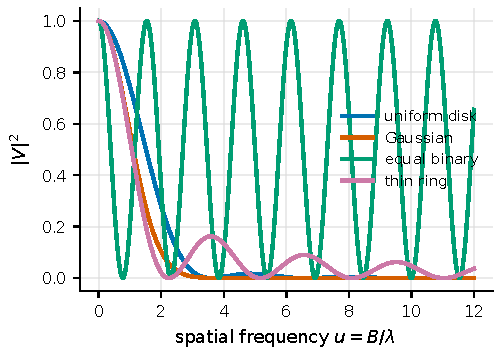
\includegraphics[width=0.88\linewidth]{figures/generated/chapter_05/ch05_vcz_visibility_models.pdf}
\caption{不同的天空亮度模型，在可见度平方 \(|V|^2\) 上留下不同的指纹。均匀圆盘出现贝塞尔型的零点，高斯源平滑衰减，等亮双星叠加一层余弦振荡，薄环则给出更密的振荡。强度干涉直接测到的正是这些曲线（的模平方），于是"读曲线"就等于"猜天空的样子"。}
\label{fig:e10-vcz-models}
\end{figure}

\section{均匀圆盘：从一条曲线量出恒星角直径}
\label{sec:e10-disk}

VCZ 定理给了通式，但天空千姿百态。要真正会用它，得从最干净的模型练手：\textbf{均匀圆盘}（uniform disk）。假设恒星是一个角直径为 \(\theta\) 的圆面，圆内表面亮度处处相等、圆外为零。这是"把恒星当成一枚均匀发光的硬币"的近似。

\textbf{推导可见度。}对圆对称的亮度分布，二维傅里叶变换退化成一维的汉克尔变换（Hankel transform）。设圆盘半径（角半径）\(a=\theta/2\)，径向空间频率 \(q=B/\lambda\)。圆对称时式 \eqref{eq:e10-vcz} 的分子写成
\[
  \int_0^{a} I_0\,J_0(2\pi q r)\,2\pi r\,\mathrm dr
  =2\pi I_0\int_0^{a}J_0(2\pi q r)\,r\,\mathrm dr,
\]
其中 \(J_0\) 是零阶贝塞尔函数（Bessel function），它是"圆对称的余弦"，正是把二维相位因子绕圆积分一圈后剩下的东西。这里用到一个标准的贝塞尔积分恒等式（任何数学物理手册都能查到）：
\[
  \int_0^{a} J_0(k r)\,r\,\mathrm dr=\frac{a}{k}\,J_1(k a),
\]
取 \(k=2\pi q\)。分母是圆盘总通量 \(I_0\cdot\pi a^2\)。两者相除：
\[
  \gamma^{(1)}
  =\frac{2\pi I_0\cdot\dfrac{a}{2\pi q}J_1(2\pi q a)}{I_0\,\pi a^2}
  =\frac{2\,J_1(2\pi q a)}{2\pi q a}.
\]
记无量纲组合 \(x\equiv 2\pi q a=2\pi\dfrac{B}{\lambda}\cdot\dfrac{\theta}{2}=\dfrac{\pi\theta B}{\lambda}\)，就得到那条著名曲线：

\begin{equation}
  V(B)=\frac{2\,J_1(x)}{x},\qquad x=\frac{\pi\,\theta\,B}{\lambda}.
  \label{eq:e10-disk}
\end{equation}
\begin{formulaexplain}
\(V(B)\)：均匀圆盘在基线 \(B\) 上的可见度。\(J_1\)：一阶贝塞尔函数。\(x=\pi\theta B/\lambda\)：无量纲"分辨程度"——越大表示星被分得越开。\(x\to0\) 时 \(2J_1(x)/x\to1\)（完全没分辨）。
\end{formulaexplain}

逐符号交代。\(V(B)\)：可见度，量纲为一，就是这条基线上的 \(\gamma^{(1)}\)（对圆盘是实数）。\(J_1(x)\)：一阶贝塞尔函数，这里我们\emph{点名引用}这个已知结果——圆形孔径的傅里叶变换总是给出 \(J_1\) 型的花样，和光学里圆孔的艾里斑（Airy pattern）同源。\(\theta\)：角直径（弧度）；\(B\)：投影基线（米）；\(\lambda\)：波长（米）。最重要的是那个组合 \(x=\pi\theta B/\lambda\)：同一颗星，基线越长或波长越短，\(x\) 越大越容易分辨；同一条基线，星越大，\(x\) 越大越敏感。

\textbf{第一零点。}曲线 \(2J_1(x)/x\) 第一次落到零，发生在 \(J_1(x)=0\) 的第一个非零根。这个根是已知的数：\(x=3.8317\)。令 \(\pi\theta B_0/\lambda=3.8317\) 解出临界基线：
\[
  B_0=\frac{3.8317}{\pi}\cdot\frac{\lambda}{\theta}=1.2197\,\frac{\lambda}{\theta}\approx1.22\,\frac{\lambda}{\theta}.
\]

\begin{equation}
  B_0\approx\frac{1.22\,\lambda}{\theta}.
  \label{eq:e10-null}
\end{equation}
\begin{formulaexplain}
\(B_0\)：可见度第一次归零的基线（米）。\(\lambda\)：波长，\(\theta\)：角直径。它标出"刚好把星分辨到第一个暗纹"所需的望远镜间距——和单口径望远镜衍射极限 \(1.22\lambda/D\) 长得一模一样，只是把口径 \(D\) 换成了基线 \(B\)。
\end{formulaexplain}

\textbf{代入真实数字。}取 VERITAS、MAGIC 常用的蓝光 \(\lambda=416\,\mathrm{nm}\)，看几种恒星大小要多长基线：
\[
  \theta=0.5\,\mathrm{mas}=0.5\times4.848\times10^{-9}\,\mathrm{rad}=2.424\times10^{-9}\,\mathrm{rad},
\]
\[
  B_0=1.22\times\frac{416\times10^{-9}}{2.424\times10^{-9}}
  =1.22\times171.6\,\mathrm{m}\approx210\,\mathrm{m}.
\]
同样地，\(\theta=1\,\mathrm{mas}\) 只要约 \(105\,\mathrm{m}\)，\(\theta=0.2\,\mathrm{mas}\) 则要约 \(520\,\mathrm{m}\)。这几个数解释了整段仪器史：Narrabri 强度干涉仪用 10--188 m 的可变基线，够测那些较亮、亚毫角秒的恒星；而要下探到几十微角秒，就得上公里级基线——这正是把大气 Cherenkov 望远镜阵列（VERITAS、MAGIC、未来的 CTAO）用作强度干涉仪的动机 \citep{1967MNRAS.137..375H,2020NatAs...4.1164A}。

\begin{figure}[tbp]
\centering
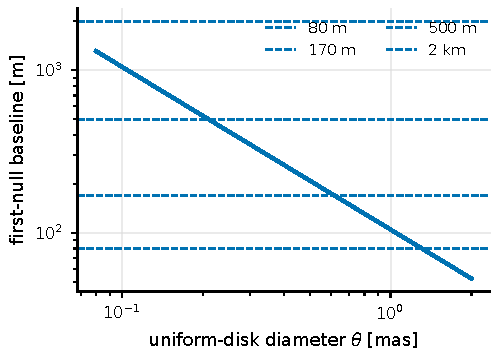
\includegraphics[width=0.86\linewidth]{figures/generated/chapter_05/ch05_uniform_disk_resolution.pdf}
\caption{均匀圆盘在 \(\lambda=416\,\mathrm{nm}\) 下的第一零点基线随角直径的变化。0.5 mas 的恒星要约 210 m 才到第一个零点，0.1 mas 量级的目标则需要公里级基线——这就是长基线 Cherenkov 阵列对蓝光强度干涉格外有吸引力的原因。}
\label{fig:e10-disk-resolution}
\end{figure}

一句实用提醒：观测时最有信息量的往往\emph{不}是零点本身，而是零点之前那段"下降区"。短基线处各种角直径的曲线几乎都贴在 \(|V|^2\approx1\)，分不出差别；零点之后 \(|V|^2\) 太低，系统误差和背景容易淹没信号；唯有下降区既有可观信号、又对 \(\theta\) 敏感。所以设计观测的第一件事，就是把目标模型的 \(|V(B)|^2\) 画出来，让基线覆盖住这段下降区（见图 \ref{fig:e10-vcz-models}）。

\section{空间 HBT：不合束，只比强度抖动同不同步}
\label{sec:e10-hbt}

到这里我们一直在谈一阶相干 \(\gamma^{(1)}\) 和复可见度——那是振幅干涉仪测的东西，需要把两束光在光学上小心地合到一起。强度干涉走的是另一条路，它连束都不合，只在探测之后比较两路\emph{强度}的抖动同不同步。凭什么这样也能测出 \(|V|\)？答案是第 \ref{chap:e08} 章的 Siegert 关系。

第 \ref{chap:e08} 章我们对同一路光、不同时刻建立了 \(g^{(2)}=1+\zeta|g^{(1)}|^2\)：热光（混沌光）的强度会成团扎堆（光子聚束），而聚束的强弱正比于一阶相干度的模平方。这条关系对"两路光、同一时刻"照样成立，只要把时间通道换成空间通道：

\begin{equation}
  g_{12}^{(2)}(0)-1=\zeta\,\big|\gamma_{12}^{(1)}\big|^2=\zeta\,\big|V(B)\big|^2 .
  \label{eq:e10-siegert}
\end{equation}
\begin{formulaexplain}
\(g_{12}^{(2)}(0)-1\)：两台望远镜零延迟强度相关的"超出量"（相对随机符合的额外扎堆）。\(\zeta\)：稀释因子（时间响应、带宽、偏振、背景一起拉低聚束高度）。\(|V(B)|^2\)：可见度模平方——正是我们想要的天体结构。
\end{formulaexplain}

逐符号说明。\(g_{12}^{(2)}(0)\)：两路强度在零时间延迟下的归一化二阶相关；减去 1，得到相对于"完全随机、毫不相关"基线的超出。\(\zeta\)（量纲为一，介于 0 和 1）：把有限探测器时间宽度、有限光学带宽、未选偏振、背景光稀释等一切"把聚束峰压平"的因素打包进来。\(|\gamma_{12}^{(1)}|^2\)：对热光/高斯混沌光，它就等于 \(|V(B)|^2\)。这条式子是空间 HBT（Hanbury Brown--Twiss）的心脏：\textbf{两台望远镜强度抖动的同步程度，直接给出可见度模平方}，全程不需要把电场合束 \citep{1956Natur.177...27B}。

\textbf{观测模型。}真机上数据分析常把式 \eqref{eq:e10-siegert} 写成一个把"仪器、背景、天体"三样东西分开的模型。其实这一步就是\emph{把式 \eqref{eq:e10-siegert} 里那个笼统的稀释因子 \(\zeta\) 拆开写清楚}——把它分成 \(\zeta=N_0\,f_1 f_2\)：\(N_0\) 收纳仪器一侧的稀释（探测器时间响应、带宽、偏振，即后面式 \eqref{eq:e10-n0} 那一项），\(f_1 f_2\) 收纳背景一侧的稀释（目标光子在两台望远镜总计数里的占比）。于是稀释因子并没有消失，只是被拆成"仪器 \(\times\) 背景"两块，各自可以单独标定：

\begin{equation}
  C_{12}(B)\equiv g_{12}^{(2)}(0)-1=N_0\,f_1 f_2\,\big|V(B)\big|^2 .
  \label{eq:e10-model}
\end{equation}
\begin{formulaexplain}
\(C_{12}\)：实测到的相关峰高度。\(N_0\)：零基线仪器响应（星没被空间分辨时应有的聚束高度）。\(f_1,f_2\)：两台望远镜里目标光子占总计数的比例。\(|V|^2\)：天体结构项。三者相乘，把仪器、背景、天空干净地拆开。
\end{formulaexplain}

逐符号：\(C_{12}(B)\) 是基线 \(B\) 上的相关峰幅度（量纲为一）；\(N_0\) 是\emph{零基线}相关幅度，即两台望远镜挨在一起、星完全没被分辨（\(|V|=1\)）时应有的聚束高度，它把探测响应后的仪器效应全收进去；\(f_1,f_2\)（量纲为一，\(\le1\)）是各台望远镜里真正来自目标的光子占比——月光、夜天光、邻星把它拉低；\(V(B)\) 是式 \eqref{eq:e10-disk}（或更复杂模型）给出的归一化可见度。这个乘积结构让分析可以逐项校准：\(|V|^2\) 随基线变，\(f_1f_2\) 随背景变，\(N_0\) 是仪器的"身份证"。

\textbf{零基线幅度有多小。}对未选偏振的热光，若探测器有效时间宽度为 \(\Delta t_{\rm eff}\)、光学带宽为 \(\Delta\nu\)，零基线幅度的数量级是

\begin{equation}
  N_0\sim\frac{1}{2\,\Delta\nu\,\Delta t_{\rm eff}},\qquad
  \Delta\nu\simeq\frac{c\,\Delta\lambda}{\lambda^2}.
  \label{eq:e10-n0}
\end{equation}
\begin{formulaexplain}
\(N_0\)：星未被分辨时的聚束峰高度。\(\Delta\nu\)：光学频率带宽（Hz）。\(\Delta t_{\rm eff}\)：电子学有效时间宽度（s）。分母里的 \(2\) 是未选偏振（两个偏振模式）带来的稀释。带宽越宽、时间响应越慢，热光聚束峰被平均得越低。
\end{formulaexplain}

物理上这很好理解（可回想第 \ref{chap:e02} 章带宽与相干时间互为倒数）：聚束这件事只在一个相干时间 \(\tau_c\sim1/\Delta\nu\) 之内才"看得见"，而探测器要花 \(\Delta t_{\rm eff}\) 去积分。探测器远慢于相干时间时（\(\Delta t_{\rm eff}\gg\tau_c\)），一次积分里塞进了 \(\sim\Delta t_{\rm eff}/\tau_c=\Delta\nu\,\Delta t_{\rm eff}\) 个互不相关的相干块，聚束信号被这么多块一平均就摊薄了，于是 \(N_0\) 反比于这个大数。

\textbf{代入 VERITAS 的真实参数}（\(\lambda=416\,\mathrm{nm}\)、\(\Delta\lambda=13\,\mathrm{nm}\)、\(\Delta t_{\rm eff}\sim4\,\mathrm{ns}\)）：先算带宽
\[
  \Delta\nu\simeq\frac{c\,\Delta\lambda}{\lambda^2}
  =\frac{(3\times10^8)\,(13\times10^{-9})}{(416\times10^{-9})^2}
  =\frac{3.9}{1.73\times10^{-13}}\ \mathrm{Hz}\approx2.3\times10^{13}\,\mathrm{Hz},
\]
再代进 \(N_0\)：
\[
  N_0\sim\frac{1}{2\,(2.3\times10^{13})\,(4\times10^{-9})}
  =\frac{1}{1.8\times10^{5}}\approx5\times10^{-6}.
\]
数量级是百万分之几。真机拟合得到的 \(N_0\approx1.25\times10^{-6}\)，比粗估略低——因为真实的滤光片形状、电子响应和系统效率还要再把峰压一压。无论如何，结论令人肃然：\textbf{热光的聚束峰只有百万分之一量级}，要在这么低的信号上量恒星，靠的是长时间积累和对 \(N_0\) 的严苛标定（图 \ref{fig:e10-zero-baseline}）\citep{2020NatAs...4.1164A}。

\begin{figure}[tbp]
\centering
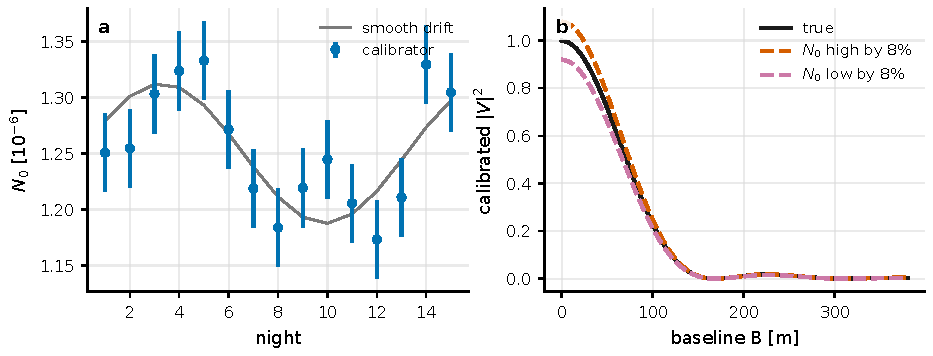
\includegraphics[width=0.92\linewidth]{figures/generated/chapter_05/ch05_zero_baseline_calibration.pdf}
\caption{零基线幅度 \(N_0\) 的标定会直接搬运到 \(|V|^2\) 上。左：校准星给出的夜间 \(N_0\) 漂移。右：\(N_0\) 若偏高或偏低 8\%，\emph{所有}基线上的 \(|V|^2\) 都被整体拉伸，进而把角直径、边缘昏暗或扁率的拟合推向错误值。这解释了为什么 \(N_0\) 是强度干涉里最要命的一项系统。}
\label{fig:e10-zero-baseline}
\end{figure}

\section{相位缺失：软肋，也是护身符}
\label{sec:e10-phase}

强度干涉只测 \(|V|^2\)——式 \eqref{eq:e10-model} 里那个模平方——把复可见度 \(\gamma_{12}^{(1)}\) 的辐角（傅里叶相位）扔掉了。这带来一个原理性的模糊。

\textbf{镜像退化。}考虑一幅亮度分布 \(I(l,m)\) 和它绕中心翻转后的镜像 \(I(-l,-m)\)。用式 \eqref{eq:e10-vcz} 做傅里叶变换，实亮度分布的傅里叶变换满足 \(\gamma(-u,-v)=\gamma^{\ast}(u,v)\)（因为 \(I\) 是实的）；而镜像分布的傅里叶变换恰好是原来那个的复共轭。取模平方时，复共轭不改变模，于是
\[
  \big|V_{\text{原图}}(u,v)\big|^2=\big|V_{\text{镜像}}(u,v)\big|^2 .
\]
两幅长得不一样的天空，给出\emph{完全相同}的 \(|V|^2\)——只测模平方的仪器无法区分它们（图 \ref{fig:e10-phase-ambiguity}）。这就是为什么"从 \(|V|^2\) 直接成像"是一件需要额外信息（二维 \(u,v\) 覆盖、物理先验、三阶相关或相位恢复算法）的难事，我们把真正的成像留到第 \ref{chap:e11} 章。

\begin{figure}[tbp]
\centering
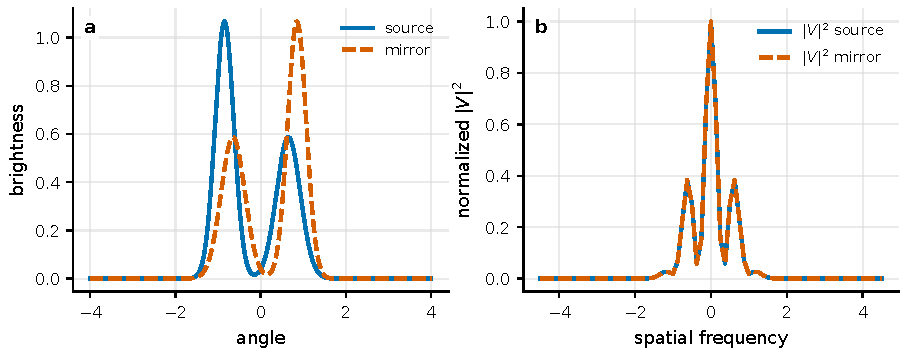
\includegraphics[width=0.92\linewidth]{figures/generated/chapter_05/ch05_phase_ambiguity.pdf}
\caption{只测 \(|V|^2\) 会丢掉傅里叶相位。左：一个源和它的镜像源，亮度分布明显不同。右：两者的 \(|V|^2\) 完全重合。强度干涉要成像，必须靠二维 \(u,v\) 覆盖、物理先验、三阶（闭合）相关或相位恢复算法来打破这类退化。}
\label{fig:e10-phase-ambiguity}
\end{figure}

\textbf{丢相位换来了什么？}答案是：对光程和大气抖动近乎免疫——这正是让 Cherenkov 望远镜能做干涉的根本原因。振幅干涉仪要把两束光在光学上合到一起看条纹，必须把两条光路的\emph{光程}稳定到波长的一小部分（几十纳米量级）；而大气湍流让波前不停地起伏，给每台望远镜叠加一个随机的、快速跳动的光程偏移，术语叫\textbf{活塞相位}（piston）。piston 对振幅干涉是致命的，条纹会被抖没。

强度干涉却几乎不在乎它。理由在于：它比较的是两路\emph{强度}的抖动同不同步，只需要把两路\emph{电子信号}在时间上对齐到探测响应时间的一小部分即可。对 \(1\,\mathrm{GHz}\) 电子带宽，时间分辨约 1 ns，对应的光程容差是 \(c\times1\,\mathrm{ns}\approx30\,\mathrm{cm}\)——要几厘米到几十厘米的路径误差才会明显降低相关。大气 piston 那点纳米到微米量级的光程抖动，落在这个容差里连零头都算不上。换句话说，\textbf{强度干涉用"丢掉相位"这个代价，买来了"不怕大气、不需精密光程"这个巨大便利}。正因如此，那些光学像质远达不到专业干涉仪水准、却拥有大口径和快探测器的 Cherenkov 望远镜，反而成了理想的强度干涉阵列 \citep{2006ApJ...649..399L,2024MNRAS.529.4387A}。

\section{本章要点}
\label{sec:e10-summary}

\begin{itemize}
  \item \textbf{几何定角尺度。}投影基线 \(\bm B_\perp\) 给程差 \(\bm B\cdot\bm s\)，空间频率 \(u=B_x/\lambda,\ v=B_y/\lambda\) 是无量纲的"波长数"。百米基线、蓝绿光对应约 1 mas（\(B/\lambda=2\times10^8\)，倒过来 \(\lambda/B\approx1\,\mathrm{mas}\)）。分辨本领由基线、而非口径决定。
  \item \textbf{相干度是一支复箭头。}一阶空间相干度 \(\gamma_{12}^{(1)}=\langle E_1^\ast E_2\rangle/\sqrt{\langle|E_1|^2\rangle\langle|E_2|^2\rangle}\)：模给相干强弱，辐角给傅里叶相位。
  \item \textbf{van Cittert--Zernike 定理。}非相干远场源的 \(\gamma^{(1)}(u,v)\) 就是归一化天空亮度的傅里叶分量（式 \eqref{eq:e10-vcz}）。短基线看粗结构、长基线看细结构。成立要四条：源内非相干、窄带、小视场、源不变。
  \item \textbf{均匀圆盘。}\(V(B)=2J_1(x)/x,\ x=\pi\theta B/\lambda\)（一阶贝塞尔函数）；第一零点 \(x=3.8317\) 给 \(B_0\approx1.22\lambda/\theta\)。416 nm、0.5 mas \(\Rightarrow\) 约 210 m。最有信息的是零点前的下降区。
  \item \textbf{空间 HBT。}把第 \ref{chap:e08} 章 Siegert 关系搬到空间通道：\(g_{12}^{(2)}(0)-1=\zeta|V(B)|^2\)；不合束、只比强度抖动同步度就能测 \(|V|^2\)。观测模型 \(C_{12}=N_0 f_1 f_2|V|^2\)，零基线幅度 \(N_0\sim1/(2\Delta\nu\Delta t_{\rm eff})\)；VERITAS 参数给约 \(5\times10^{-6}\)，实测 \(1.25\times10^{-6}\)。
  \item \textbf{相位缺失是双刃剑。}只测 \(|V|^2\)，镜像亮度分布 \(I(-l,-m)\) 给同样的 \(|V|^2\)（退化）；但代价换来对光程/大气 piston 的免疫——这正是 Cherenkov 望远镜能做干涉的原因。成像留到第 \ref{chap:e11} 章。
\end{itemize}

\medskip
\noindent\textbf{想一想。}
\begin{itemize}
  \item 若把观测波长从 416 nm 换成 640 nm 的红光，同一颗 0.5 mas 恒星的第一零点基线会变长还是变短？变到多少米？
  \item 两台望远镜里目标光子占比若从 70\% 掉到 50\%，式 \eqref{eq:e10-model} 里的相关峰会被压到原来的几分之几？要恢复同样显著性，积分时间大致要加多少倍（回想 SNR 随时间只按平方根增长）？
  \item 为什么"窄带"是 VCZ 定理的必要条件？如果带宽很宽，式 \eqref{eq:e10-uv} 会出什么问题？
\end{itemize}

\chapter{从可见度到成像：角直径、多基线与 uv 覆盖}
\label{chap:e11}

\begin{chapteropening}
上一章我们把两台相距很远的望远镜连在一起，证明了它们记录的强度涨落是否同步，直接给出天体在某条基线上的平方可见度 \(|V(B)|^2\)——一个介于 0 和 1 之间的纯数字。可是天文学家要的从来不是一个数字，而是"这颗星有多大""它是圆的还是扁的""它是一颗星还是两颗贴在一起""表面有没有亮斑"，最终甚至是一张\emph{图}。本章要做的，就是把单条基线上那个孤零零的 \(|V|^2\) 一步步变成真正的科学产品：先算清楚"要测到这个数字，需要多亮的星、多大的镜子、多长的曝光"（信噪比）；再学会判断"这一夜的相关峰到底是真信号还是仪器捣鬼"（可行性与误差）；然后把两台望远镜扩成一个阵列，让地球自转帮我们在 Fourier 平面上画出一片二维覆盖（多基线与 uv 覆盖）；最后面对强度干涉与生俱来的软肋——相位丢了——看看闭合相位、相位恢复和物理先验怎样把图像重新拼回来。走完这一章，你会明白为什么一套 1960 年代被判"死刑"的老方法，会在今天的 Cherenkov 望远镜阵列上原地复活。
\end{chapteropening}

\section{要测到这个数字，得付出多少：强度干涉的信噪比}
\label{sec:e11-snr}

先把上一章的结论接住。对热光（thermal light，即普通恒星那种混沌光）而言，两台望远镜零延迟强度相关的超额，正比于该基线上的平方可见度；写成可以直接拟合观测数据的模型，就是第 \ref{chap:e10} 章得到的
\begin{equation}
  C_{12}(B)\equiv g_{12}^{(2)}(0)-1 = N_0\,f_1 f_2\,\big|V(B)\big|^2 ,
  \label{eq:e11-correlation-model}
\end{equation}
\begin{formulaexplain}
\(C_{12}\) 是基线 \(B\) 上测到的相关峰高度；\(N_0\) 是"零基线"仪器响应（源没被空间分辨时的聚束峰高）；\(f_1,f_2\) 是两台望远镜里目标光子占总计数的比例；\(|V|^2\) 是纯粹的天体结构项。仪器、背景、天体被干净地分成三段。
\end{formulaexplain}
这里 \(C_{12}\) 无量纲；\(N_0\) 也无量纲，量级在百万分之一（\(\sim10^{-6}\)）；\(f_1,f_2\) 是 0 到 1 之间的分数；\(|V(B)|^2\) 是我们真正想要的科学量。麻烦在于：这个信号\emph{实在太浅}。峰高只有 \(10^{-6}\) 到 \(10^{-3}\)，意味着我们要在一片几乎全是随机符合的背景上，去分辨百万分之一的一个隆起。能不能测到，取决于信噪比。

\paragraph{信噪比公式：逐个符号拆开}
\label{sec:e11-snr-formula}

Hanbury Brown 当年为 Narrabri 恒星强度干涉仪推导的双望远镜信噪比，今天仍是设计任何一次强度干涉观测的第一张算盘。它写成
\begin{equation}
  \left(\frac{S}{N}\right)_{\rm rms}
  = A\,\alpha\,n\,\big|\gamma_{12}\big|^2
  \left(\frac{\Delta f\,T}{2}\right)^{1/2}.
  \label{eq:e11-snr}
\end{equation}
\begin{formulaexplain}
\(A\) 是每台望远镜收集面积，\(\alpha\) 是探测效率，\(n\) 是光子谱流量，\(|\gamma_{12}|^2=|V|^2\) 是平方可见度，\(\Delta f\) 是电子带宽，\(T\) 是积分时间。信噪比\emph{线性}地跟着光子数走，却只按带宽和时间的\emph{平方根}长。
\end{formulaexplain}

这条式子每一个符号都值得单独交代，因为它们各自对应一个可以在设计观测时拧的"旋钮"：

\begin{itemize}
  \item \(A\)：每台望远镜的收集面积，单位 \({\rm cm^2}\)。这里为什么是 \(A\) 的\emph{一次}方，而不是 \(A^2\)？分子分母各走一步就清楚了：信号（那个符合计数超额）正比于两路总计数的乘积，也就是 \(\propto A_1 A_2\)；但噪声（散粒噪声底）也随两路的总计数一起涨，做除法时抵掉了一半的面积依赖，最后信噪比 \(\propto\sqrt{A_1 A_2}\)——两台等面积（\(A_1=A_2=A\)）时正好是一次 \(A\)，即两面积的\emph{几何平均}。换个等价说法：真正进入信噪比的物理量是每模式的占据数（简并度）\(\delta=A\,\alpha\,n\)，它本来就只带一次 \(A\)。抓住直觉即可：镜子越大，进来的目标光子越多，浅浅的相关峰就越站得住。
  \item \(\alpha\)：总光子探测效率，无量纲，是一串损失的乘积——镜面反射率 \(\times\) 滤光片透过率 \(\times\) 光电阴极量子效率 \(\times\) 读出/触发损失。典型现代蓝光系统 \(\alpha\sim0.2\)–\(0.3\)。
  \item \(n\)：目标在观测波段的\textbf{光子谱流量}（photon spectral flux），单位 \({\rm photons\,s^{-1}\,cm^{-2}\,Hz^{-1}}\)。它直接对应恒星的亮度——这是全式里唯一由"天上那颗星有多亮"决定、我们\emph{无法}用工程手段改变的量。
  \item \(|\gamma_{12}|^2=|V(B)|^2\)：这条基线上的平方可见度，无量纲，就是我们要测的科学量本身。注意信噪比正比于 \(|\gamma|^2\) 而非 \(|\gamma|\)：越靠近可见度零点、信号越弱的地方，越难测——这是强度干涉的宿命。
  \item \(\Delta f\)：电子相关带宽，单位 Hz，即相关器能分辨的最快时间结构 \(\sim1/\Delta f\)。注意它\emph{不是}光学滤光片带宽，而是探测器加电子学的响应带宽，现代系统在 \(10^8\)–\(10^9\,{\rm Hz}\)。
  \item \(T\)：积分时间，单位 s。
\end{itemize}

\paragraph{那个平方根是从哪儿来的}
\label{sec:e11-snr-sqrt}

式 \eqref{eq:e11-snr} 里最该讲清楚的，是括号里的 \((\Delta f\,T/2)^{1/2}\)——为什么信号明明是"测一个固定的相关峰高"，最后却冒出一个平方根？这不是魔法，而是第 \ref{chap:e03} 章那条"多次独立测量取平均，误差按 \(1/\sqrt{N}\) 缩小"的老结论在这里的直接兑现。我们把它一步步走出来。

\textbf{第一步：一次测量能独立采样多少次？}电子带宽 \(\Delta f\) 意味着相关器每隔约 \(1/\Delta f\) 的时间才能给出一个\emph{互相独立}的强度乘积样本（更快的结构它分辨不了，更慢的则被平滑掉）。于是在积分时间 \(T\) 里，独立样本的数目大约是
\[
  M \sim \Delta f\,T .
\]
取 \(\Delta f=1\,{\rm GHz}=10^9\,{\rm Hz}\)、\(T=5\,{\rm hr}=1.8\times10^4\,{\rm s}\)，就是 \(M\sim1.8\times10^{13}\) 次独立测量——一个天文数字。

\textbf{第二步：把 \(M\) 次独立测量平均起来。}每一次强度乘积的测量都被散粒噪声（shot noise）搞得上下乱跳，单次的信噪比极差。但它们彼此独立，于是按第 \ref{chap:e03} 章的中心极限结论，把 \(M\) 次取平均后，随机噪声的相对起伏缩小为原来的 \(1/\sqrt{M}\)。信号（那个真实的相关峰高）在平均中保持不变，噪声却被压低 \(\sqrt{M}\) 倍，所以
\[
  \frac{S}{N}\ \propto\ \sqrt{M}\ \sim\ \sqrt{\Delta f\,T}.
\]

\textbf{第三步：凑出前面的系数。}信号本身正比于\emph{被相关的目标光子率}，也就是 \(A\alpha n\)（面积 \(\times\) 效率 \(\times\) 谱流量）再乘上结构因子 \(|\gamma_{12}|^2\)；那个 \(1/\sqrt2\) 是热光两个偏振模式未被投影时的稀释因子（与上一章 \(N_0\sim1/(2\Delta\nu\Delta t)\) 里的同一个 \(1/2\) 同源）。把三步拼起来，就还原出式 \eqref{eq:e11-snr}。整个平方根的来历只有一句话：\emph{强度干涉靠的是在海量独立样本上做平均，而平均对随机噪声的压制，永远只有平方根那么快。}

\paragraph{两条必须记住的结论}
\label{sec:e11-snr-lessons}

式 \eqref{eq:e11-snr} 的结构里藏着两条会反复决定观测成败的经验：

\textbf{结论一：信噪比\emph{线性}地正比于光子谱流量、收集面积和效率。}三个因子 \(A\alpha n\) 都是一次方。这就是为什么强度干涉天生偏爱\emph{亮星}和\emph{大镜面}：星每暗一个星等，光子谱流量 \(n\) 就乘以 \(10^{-0.4}\simeq0.398\)，信噪比也直接打成四折；而把镜面口径从 \(6.5\,{\rm m}\)（Narrabri）换成 \(12\,{\rm m}\)（VERITAS），面积翻了 3.4 倍，信噪比同样翻 3.4 倍。天体的亮度我们改不了，但镜面和效率是工程能砸钱的地方——这正是"为什么要用大望远镜做强度干涉"的定量答案。

\textbf{结论二：信噪比只按 \((\Delta f\,T)^{1/2}\) 增长，慢得令人心痛。}平方根意味着\emph{曝光翻两番、信噪比才翻一番}：把观测从 5 小时加到 20 小时（\(\times4\)），信噪比只从比如 \(3\sigma\) 变成 \(6\sigma\)；把电子带宽从 \(250\,{\rm MHz}\) 提到 \(1\,{\rm GHz}\)（\(\times4\)），也只换来 2 倍。这解释了强度干涉长期的困境：想靠"多熬几夜"把暗星拉进探测范围，代价高得离谱；真正的突破口在结论一里那几个线性因子——更大的镜子、更高的效率、更亮的目标。

顺带说清一件常让初学者困惑的事：式 \eqref{eq:e11-snr} 里\emph{没有}光学滤光片带宽 \(\Delta\nu_{\rm opt}\)。这不是遗漏。关键是要记住 \(n\) 的定义（第 40 行那条）：它是\emph{每赫兹}的光子谱流量，量纲 \({\rm photons\,s^{-1}\,cm^{-2}\,Hz^{-1}}\)——它\emph{本身不随滤光片宽度变}。收窄滤光片，改变的是进来的\emph{总}光子数（\(\propto n\,\Delta\nu_{\rm opt}\)），而不是每赫兹的 \(n\)。那为什么总光子数少了、信噪比却不掉？因为在探测器远慢于光学相干时间的极限下（第 \ref{chap:e05} 章我们算过可见光 \(\tau_c<1\,{\rm ps}\)，而探测器响应在 ns 量级），收窄滤光片会同时按比例抬高相干时间 \(\tau_c\simeq1/\Delta\nu_{\rm opt}\) 与每模式的占据数（聚束峰 \(N_0\)）——总光子数下降与聚束峰上升在信噪比里恰好抵消。到头来，真正进入信噪比公式的只有\emph{与滤光片无关}的每赫兹谱流量 \(n\) 和电子带宽 \(\Delta f\)。所以窄带滤光片主要是用来\emph{压背景}的，不是用来提信号的——真实系统仍要把滤光片形状、背景和探测器响应老老实实塞进 \(N_0\) 或完整的似然函数里。

\begin{figure}[tbp]
\centering
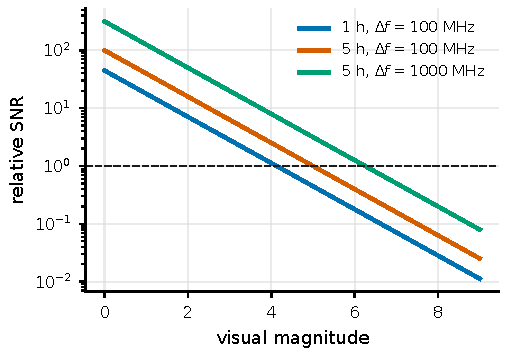
\includegraphics[width=0.86\linewidth]{figures/generated/chapter_05/ch05_snr_scaling.pdf}
\caption{强度干涉信噪比的相对标度。恒星每暗 1 等，光子谱流量约降为原来的 \(0.398\)，信噪比同比例线性下降；而积分时间和电子带宽只按平方根改善信噪比——曝光翻两番才换来信噪比翻一番。曲线未含收集面积、效率、背景稀释和 \(|V|^2\)，正是要凸显：亮星选择与高速电子学（线性因子）远比"多熬几夜"（平方根因子）划算。}
\label{fig:e11-snr-scaling}
\end{figure}

\paragraph{代入真实数字：Le Bohec--Holder 的数量级}
\label{sec:e11-snr-lebohec}

抽象公式要落地，就得代真实参数。Le~Bohec 和 Holder 在评估把 Cherenkov 阵列用于强度干涉的可行性时，做过一个经典估算 \citep{2006ApJ...649..399L}：取两台 \(A=100\,{\rm m^2}\) 的望远镜、探测效率 \(\alpha=0.3\)、电子带宽 \(\Delta f=1\,{\rm GHz}\)、积分时间 \(T=5\,{\rm hr}\)，在可见度平方 \(|\gamma_{12}|^2=0.5\) 的基线处，能以 \(5\sigma\) 显著性测到大约 \(V=6.7\) 等的恒星；对更亮的 \(V=5\) 等星，角直径精度可以做到几个百分点。对照上一节两条结论：这个 \(V=6.7\) 的极限灵敏度，几乎全由那几个线性因子（大面积、高效率、GHz 带宽）撑起来；想再往暗里推一等，靠的不是加时间（平方根，太贵），而是继续加面积和效率。

拿它和历史仪器对照，数量级立刻活了起来。Narrabri 用的是两台直径 \(6.5\,{\rm m}\) 的光收集器、\(443\,{\rm nm}\) 中心波长、\(10\,{\rm nm}\) 滤光片、光电阴极量子效率约 25\%、有效电子带宽仅约 \(60\,{\rm MHz}\) \citep{1967MNRAS.137..375H,1974MNRAS.167..121H,1974iiia.book.....H}。把这些数字代进式 \eqref{eq:e11-snr}，就明白为什么它的样本只能限于最亮的那批星（视星等大致 \(B<2.5\)）：面积比现代小、带宽小了一个多量级，几个线性和平方根因子叠加起来，把灵敏度死死钉在了亮星上。而 VERITAS 用四台 \(12\,{\rm m}\) 望远镜、250 MS/s 采样加离线相关，即使在接近满月、无法做伽马观测的"废时间"里，也能在几小时内测出恒星直径 \citep{2020NatAs...4.1164A}——这正是那几个线性因子（面积 \(\times3.4\)、效率提升）与更宽电子带宽联手的结果。

\section{怎样判断一次观测是真信号还是仪器捣鬼}
\label{sec:e11-feasibility}

信噪比公式告诉你"够不够亮、够不够久"，但它默认噪声是干净的白噪声。真实观测里最要命的敌人不是白噪声，而是两类会伪装成信号的东西：\emph{背景光}和\emph{系统相关}。因为真信号本身只有百万分之一到千分之一那么浅，任何一点没被识破的系统效应，都可能把角直径拟合带进沟里。

\paragraph{背景以两种方式同时伤人}
\label{sec:e11-background}

月光、夜天光（night-sky background）、被展宽的点扩散函数（PSF）里混进的相邻星光、探测器暗电流——这些非目标光子统称背景。它们伤害观测的方式\emph{有两条，而且同时起作用}：

\textbf{第一条，增加散粒噪声。}背景光子也要被探测、也要参与符合计数，它们贡献的散粒噪声直接抬高式 \eqref{eq:e11-snr} 分母里的噪声底，把信噪比往下拽。

\textbf{第二条，乘一个 \(f_1f_2\) 稀释因子。}回看式 \eqref{eq:e11-correlation-model}：相关峰被乘上了 \(f_1f_2\)，即两台望远镜里目标光子占总光子的比例之积。这一条更阴险，因为它是\emph{乘性}的。举个数字：若每台望远镜里目标光子只占 70\%（\(f_1=f_2=0.7\)），相关振幅就被压到
\[
  f_1 f_2 = 0.7\times0.7 = 0.49,
\]
只剩下不到一半。要把这半截信号找回同样的显著性，按信噪比的平方根标度，得把积分时间加到大约 4 倍——而积分越久，各种缓慢的系统漂移越容易冒头。Le~Bohec 和 Holder 早就指出，Cherenkov 望远镜那种 \(0.05^\circ\) 量级的宽光学 PSF 会让夜天光成为暗星灵敏度的边界；现代 VERITAS 的分析也必须专门修正夜天光背景和暗电流，否则角直径能被拉偏约 10\% 量级 \citep{2006ApJ...649..399L,2020NatAs...4.1164A,2025ApJ...995..191A}。这就是为什么窄带滤光片和小视场光阑在强度干涉里如此重要：它们不提信号，却是把 \(f_1,f_2\) 顶到接近 1 的关键。

\begin{figure}[tbp]
\centering
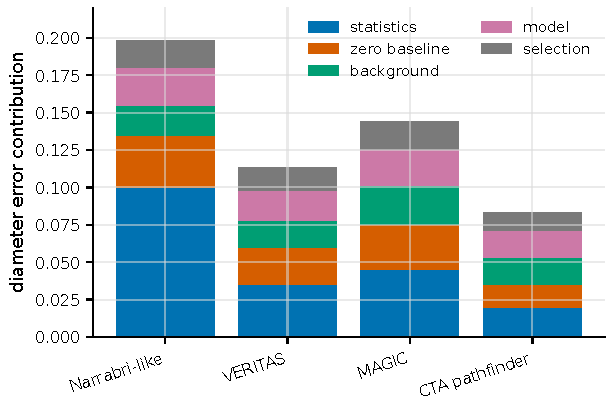
\includegraphics[width=0.82\linewidth]{figures/generated/chapter_05/ch05_error_budget.pdf}
\caption{强度干涉角直径误差预算的组成。统计误差（photon noise）会随光子数和积分时间按平方根下降，但零基线定标、背景稀释、恒星大气模型和天气/选择函数会共同筑起一道系统误差地板。现代阵列能不能出科学结果，取决于这些系统项能否和 photon noise 一起被诚实地写进似然函数——而不是被时间的平方根"熬"掉。}
\label{fig:e11-error-budget}
\end{figure}

\paragraph{系统相关比白噪声更危险}
\label{sec:e11-systematics}

白噪声至少是"公平"的：它随机，能靠平均压下去。真正让人夜不能寐的是\textbf{系统相关}（systematic correlation）——两路信号里某种\emph{非天体}的、却又同步的东西。地面反射、共用的时钟、电源纹波、温度联动、光纤串扰，都可能在两路电信号里注入一个假的相关峰。它之所以比白噪声危险，就因为真信号本来只有 \(10^{-6}\) 到 \(10^{-3}\)：白噪声再大，平均后也趋于零；而一个哪怕只有 \(10^{-5}\) 的系统相关，却不会被平均掉，它会稳稳地坐在那里，冒充成一个"可见度"。

对付它没有单一妙招，只有一整套交叉检验。下面这几条是强度干涉分析里的标准动作，值得当作检查清单背下来：

\begin{itemize}
  \item \textbf{远离零延迟处必须为零。}真正的热光聚束峰只出现在两路信号的\emph{时间对齐}处；把相对延迟拉到远离零的地方，相关应当归零。若那里还有残留，就是系统相关在作祟。
  \item \textbf{换通道或人为时移后峰应消失。}把两路信号互换、或故意插入一个不物理的时间偏移，真信号峰会随之移动或消失；如果峰纹丝不动，它就不是天上来的。
  \item \textbf{零基线响应 \(N_0\) 要处处一致。}用不同望远镜对、不同夜晚、不同月距、不同电子链路去测同一个"零基线"聚束高度，得到的 \(N_0\) 应当彼此吻合。\(N_0\) 一旦系统性偏移，式 \eqref{eq:e11-correlation-model} 里所有基线的 \(|V|^2\) 都会被整体拉伸，角直径、边缘昏暗、扁率全部跟着错。
  \item \textbf{\(|V|^2\) 应随\emph{基线}变，而不随电流变。}同一目标的可见度，只应当是投影基线 \(B\) 的函数；如果它反而跟着 PMT 阳极电流、环境温度或电子增益一起漂，那漂的就是仪器，不是恒星。
\end{itemize}

MAGIC 的强度干涉系统（MAGIC-SII）是把这套纪律工程化的好例子：它复用常规相机像素、加窄带滤光片、用 VCSEL 模拟光纤把信号传出、聚合电子带宽约 \(110\,{\rm MHz}\)、并用 GPU 实时无死时间（deadtime-free）相关器在线求相关，最终报告了 22 颗恒星的直径 \citep{2024MNRAS.529.4387A}。它把限制从"望远镜面积"推向了"工程稳定性与校准体系"——恰好印证：当信号浅到百万分之一，能不能压住系统相关，往往比镜子多大更决定成败。

\begin{figure}[tbp]
\centering
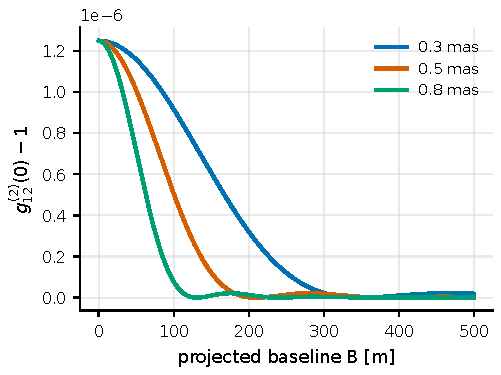
\includegraphics[width=0.86\linewidth]{figures/generated/chapter_05/ch05_sii_signal_vs_baseline.pdf}
\caption{用 \(C_{12}=N_0|V|^2\)（\(N_0\) 取 \(1.25\times10^{-6}\) 的现代蓝光系统量级）估算的强度干涉信号随基线的变化。角直径越大的星，\(|V|^2\) 越早随基线下降并出现零点；因此同一组基线对 0.8 mas 的星比对 0.3 mas 的星更敏感。观测设计的第一件事，就是照着目标的这条曲线，把基线摆在"下降区"——那里既有可观信号，又对角直径最敏感。}
\label{fig:e11-sii-signal}
\end{figure}

\section{从两台到一片：多基线与 uv 覆盖}
\label{sec:e11-uv}

两台望远镜，无论熬多久，也只能给你\emph{一条}投影基线上的一个 \(|V|^2\)。而上一章的 van~Cittert--Zernike 定理告诉我们，天体图像是它在整个 \((u,v)\) 平面上可见度的 Fourier 逆变换。所以要从"一个数字"走向"一张图"，唯一的出路是\emph{采到更多的空间频率}。这一节讲三件事怎样合力把采样从一个点铺成一整片。

\paragraph{望远镜数一多，基线数就爆炸}
\label{sec:e11-baseline-count}

第一件事最简单：多放望远镜。若阵列有 \(N\) 台望远镜，任取两台就构成一条基线，同时可形成的基线数是"从 \(N\) 里取 2"的组合数
\begin{equation}
  N_{\rm base}=\binom{N}{2}=\frac{N(N-1)}{2}.
  \label{eq:e11-baseline-number}
\end{equation}
\begin{formulaexplain}
\(N_{\rm base}\) 是可同时形成的望远镜对数（即基线数），\(N\) 是望远镜台数。每一对望远镜给一条独立基线，所以基线数随阵列规模近似按 \(N^2/2\) 爆炸式增长。
\end{formulaexplain}
组合数 \(\binom{N}{2}\) 的来历是标准计数：第一台有 \(N\) 种选法、第二台剩 \(N-1\) 种，但"甲乙"和"乙甲"是同一条基线要除以 2。代几个数就明白它多划算：\(N=2\) 只有 1 条基线；\(N=4\)（VERITAS）一下子有 6 条；\(N=17\) 有 136 条；而 CTAO 级别的几十到上百台望远镜，能同时给出上千条基线。基线数按 \(N^2\) 涨，是阵列望远镜相对双天线的根本优势。

这里要点出强度干涉一个\emph{独有}的甜头。振幅干涉（amplitude interferometry）要把同一束相干光在光学上分给多个合束器，每分一路就损失一份光子，路数一多信号就摊薄了。强度干涉不在光学上合束，它先把每台望远镜的光探测成\emph{电信号}，而电信号可以\textbf{无损地复制}到任意多个相关器里。于是一台望远镜的信号可以同时和其余每一台去求相关，把全部 \(N(N-1)/2\) 条基线一次拿下，完全不用在望远镜之间"分光"。对追求密集 \((u,v)\) 覆盖的成像来说，这是强度干涉方案天然的便宜。

\paragraph{让地球替你转：一条基线扫出一段轨迹}
\label{sec:e11-earth-rotation}

第二件事不花一分钱：等地球自转。一对望远镜在地面上的间隔矢量是固定的，但它\emph{投影到垂直视线的天空平面}上的分量，会随目标在天上升落而不断改变。回忆上一章的定义，空间频率就是投影基线除以波长，\(u=B_x/\lambda,\ v=B_y/\lambda\)。随着地球把目标从东边转到西边，投影基线 \((B_x,B_y)\) 连续变化，于是同一对固定的望远镜，会在一夜之内让它的采样点\emph{沿着 \((u,v)\) 平面画出一段弧线}。这套"地球自转合成孔径"（Earth-rotation synthesis）是射电干涉几十年的看家本领，在强度干涉里同样适用：只要每隔几分钟就把相关结果存一次，一个采样点就被拉成了一条轨迹。

\paragraph{多夜、多时角、多望远镜对：拼出二维覆盖}
\label{sec:e11-2d-coverage}

第三件事是把前两件反复叠加。一夜之内地球只能转过一段时角（hour angle），画出的弧线有限；但换一夜、换一个季节、把目标在不同时角下都观测一遍，弧线就一段段接上。再把阵列里\emph{每一对}望远镜的轨迹全叠在同一张 \((u,v)\) 图上——每对望远镜画一条、加上它关于原点对称的共轭点（因为真实亮度分布保证 \(V(-u,-v)=V^*(u,v)\)，负频率点同样是约束）——最终就从零零星星几个点，拼出一片二维的 \((u,v)\) 覆盖。覆盖越稠密，能区分的天体结构就越精细：稀疏采样只够拟合一个直径，稠密采样才能分辨圆盘、椭圆、双星，乃至表面亮斑 \citep{2008AIPC..984..205L,2012MNRAS.419..172N,2013APh....43..331D}。

\begin{figure}[tbp]
\centering
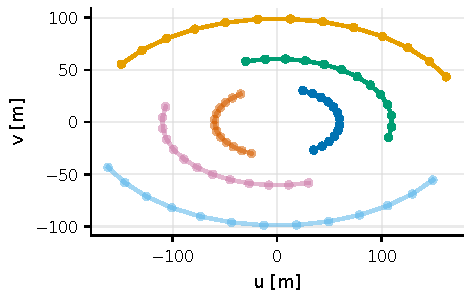
\includegraphics[width=0.82\linewidth]{figures/generated/chapter_05/ch05_uv_coverage.pdf}
\caption{固定的望远镜基线在地球自转中被投影到不同的 \((u,v)\) 位置。每条彩色轨迹代表一对望远镜在一夜时角变化中扫过的空间频率，原点对称的共轭点（虚线一侧）也是对实亮度分布的有效 Fourier 约束。多对望远镜、多夜、多时角叠加起来，采样就从孤立几点长成二维覆盖——覆盖越密，越能把圆盘、椭圆、双星和表面斑点区分开。}
\label{fig:e11-uv-coverage}
\end{figure}

\section{相位丢了怎么办：闭合相位、相位恢复与低维模型}
\label{sec:e11-phase}

到这里必须直面强度干涉与生俱来的软肋。振幅干涉直接测复可见度 \(V=|V|e^{i\phi}\)，模和相位一起拿到；而强度干涉只测\emph{强度涨落的同步程度}，得到的是 \(|V|^2\)——\textbf{相位 \(\phi\) 丢了}。这不是小事：Fourier 相位恰恰编码着"亮度往哪边偏"的信息。丢了相位最直接的后果是一种镜像退化——一个亮度分布 \(I(l,m)\) 和它的中心反演镜像 \(I(-l,-m)\)，拥有\emph{完全相同}的 \(|V|^2\)，光凭平方可见度永远分不开这两者。只测模平方，等于只知道每个空间频率上"有多少起伏"，却不知道"起伏的相位对齐在哪"。要重建真正的图像，就得设法把相位信息补回来。有三条路。

\paragraph{出路一：三阶闭合相位}
\label{sec:e11-closure}

第一条路承接第 \ref{chap:e08} 章的三阶相干函数 \(g^{(3)}\)。当年那条三阶公式落到三台望远镜 \(1,2,3\) 上时，会冒出一项
\begin{equation}
  2\,{\rm Re}\big(\gamma_{12}\,\gamma_{23}\,\gamma_{31}\big),
  \label{eq:e11-triple}
\end{equation}
\begin{formulaexplain}
\(\gamma_{12},\gamma_{23},\gamma_{31}\) 是三条边上的复相干度。它们的乘积把三条边的相位加在一起：\(\phi_{12}+\phi_{23}+\phi_{31}\)。这个"绕三角形一圈"的相位和，就是闭合相位。
\end{formulaexplain}
关键在于这个三元乘积的相位。设每台望远镜因大气或仪器引入一个未知的"活塞"相位（piston）\(\psi_i\)，它会给每条边的相位加上 \(\psi_j-\psi_i\)。把三条边绕三角形转一圈相加：
\[
  (\psi_2-\psi_1)+(\psi_3-\psi_2)+(\psi_1-\psi_3)=0.
\]
每台望远镜那个讨厌的未知相位\emph{精确抵消}了！剩下的相位和 \(\phi_{12}+\phi_{23}+\phi_{31}\) 只属于天体本身，这个量叫\textbf{闭合相位}（closure phase）。它在概念上正是振幅干涉里对付大气抖动的老武器，如今在强度干涉里以三阶相关的面貌重现，且天然免疫单台望远镜的相位漂移。

天下没有免费的午餐：三阶信号比二阶弱得多。二阶靠的是光子\emph{成对}到达的关联，三阶要求光子\emph{三个一组}同时到达，而三元组比二元组稀罕太多，误差传播也更苛刻。所以闭合相位更适合超大阵列和极亮目标，而不是每次观测的默认产品。

\paragraph{出路二：二维覆盖 + 相位恢复算法 + 物理先验}
\label{sec:e11-phase-retrieval}

第二条路绕开相位测量，直接从一片稠密的二维 \(|V|\) 分布里\emph{反解}出相位。这听起来像无中生有，但数学上并非全无希望：对一个紧支撑（compact support）的实亮度分布，其 Fourier 模与相位并非完全独立，模的解析结构（经由 Cauchy--Riemann 关系）对相位施加了约束。Gerchberg--Saxton 迭代 \citep{1966JOSA...56..441G}、MIRA 之类的正则化重建算法，就是在"符合测到的 \(|V|\)"和"满足物理先验"两个约束之间来回投影，逼出一个自洽的相位。这里的\textbf{物理先验}是命门：亮度非负、源有有限大小、亮度分布光滑、必要时套一个恒星大气模板——正是这些先验把镜像退化和无穷多的伪解筛掉。Nuñez 等人的模拟表明，在 CTA 级别的 \((u,v)\) 覆盖下，明亮热星、快速自转星、双星、带表面斑点的恒星都能被恢复到有物理意义的形状参数，但成败取决于信噪比、短基线覆盖是否足够、先验掩膜和图像正则化怎么设 \citep{2012MNRAS.419..172N,2012MNRAS.424.1006N,2014SPIE.9146E..0ZD}。

\paragraph{出路三：干脆不重建图像，用低维模型}
\label{sec:e11-low-dim}

第三条路最务实，也常常最有力：\emph{根本不做无模型的图像重建}，而是拿一个只有几个参数的物理模型去拟合 \(|V|^2\)。别忘了，只测 \(|V|^2\) 绝不等于只能测直径。对一大类低维模型——均匀圆盘（uniform disk）、椭圆圆盘、双星、边缘昏暗（limb darkening）——平方可见度已经能给出\emph{很强}的约束。均匀圆盘的可见度是 \(V(B)=2J_1(x)/x\)（\(x=\pi\theta B/\lambda\)，第 \ref{chap:e10} 章由 Bessel 函数第一零点 \(x=3.8317\) 定出角直径），扁椭圆会让零点基线随方位角变化，双星会在 \(|V|^2\) 上叠一层余弦振荡，边缘昏暗会把第一 lobe 的形状微微改样。这些差异都\emph{不需要相位}就能从 \(|V|^2\) 曲线里读出来。当科学目标是"这颗星多大、多扁、是不是双星"，而不是"给我一张模型无关的照片"时，几个参数的模型往往比费劲的相位恢复更稳、更可信。

\section{一套老方法为什么会复活：从 Narrabri 到 CTAO}
\label{sec:e11-history}

把前面所有工具串起来，就能看懂强度干涉这条曲折的技术史——它曾被判死刑，又在半个世纪后原地复活。

\textbf{Narrabri（1960s--1970s）：证明这条路走得通。}澳大利亚 Narrabri 的恒星强度干涉仪（Stellar Intensity Interferometer）是第一台完整展示这套方法科学能力的仪器。两台直径 \(6.5\,{\rm m}\) 的光收集器在 10--188 m 的可变轨道基线上工作，滤光片中心约 \(443\,{\rm nm}\)、带宽 \(10\,{\rm nm}\)，光电阴极量子效率约 25\%，有效电子带宽约 \(60\,{\rm MHz}\)。它测出了 32 颗恒星的角直径和若干双星，最小直径约 \(0.4\,{\rm mas}\) \citep{1967MNRAS.137..375H,1967MNRAS.137..393H,1974MNRAS.167..121H,1974iiia.book.....H}。但它随后停用，原因恰好是式 \eqref{eq:e11-snr} 里那几个线性因子当年都上不去：可移动的大面积光收集器造价高、低噪声高速电子学不成熟、又缺乏多基线成像能力。老方法不是错了，是当时的硬件配不上它。

\textbf{VERITAS（2019--）：老思想撞上现成的大镜子。}转机来自大气 Cherenkov 望远镜阵列。它们本是为捕捉伽马射线引发的纳秒级 Cherenkov 闪光而造，天然就有 10~m 级口径、大面积镜面、快速 PMT、长基线和可接受的光学像质——恰好是强度干涉当年求之不得的一切。VERITAS 用四台 \(12\,{\rm m}\) 望远镜同时形成 6 条基线，对 \(\beta\)~CMa 和 \(\epsilon\)~Ori 测得均匀圆盘直径 \(\theta_{\rm UD}=0.523\pm0.017\,{\rm mas}\) 和 \(0.631\pm0.017\,{\rm mas}\)，精度优于 5\%，只用了几小时，而且是在接近满月、无法做伽马观测的时段里"顺手"完成的 \citep{2020NatAs...4.1164A}。随着 \((u,v)\) 覆盖改善，它对 \(\beta\)~UMa 和快速自转星 \(\gamma\)~Cas 的后续观测，已经从"测一个半径"进到"测方向依赖的形状"：\(\gamma\)~Cas 用 6 条基线、超过 160 pair-hours 的数据测出可见光球的扁率，小轴直径约 \(0.43\,{\rm mas}\)、长短轴比约 1.28、自转轴位置角约 \(116^\circ\) \citep{2024ApJ...966...28A,2025ApJ...995..191A}。

\textbf{MAGIC-SII（2024）：把它变成一个可切换的标准模式。}MAGIC 用两台 \(17\,{\rm m}\) 抛物面望远镜、复用原有相机像素，配上 VCSEL 模拟光纤传输和 GPU 实时无死时间相关器（聚合带宽约 \(110\,{\rm MHz}\)），实现了在常规伽马观测与强度干涉模式之间快速切换，并报告了 22 颗恒星的直径 \citep{2024MNRAS.529.4387A}。它示范的不只是"能测"，而是"能作为一台成熟设备的常规副业稳定运行"。

\textbf{CTAO（在建）：走向公里基线与上千条基线。}下一代的 CTAO 把强度干涉的两大杠杆同时拉满。公里级基线在 350--450 nm 对应\emph{几十微角秒}的分辨率——比 Narrabri 精细一两个量级；而几十到上百台望远镜按式 \eqref{eq:e11-baseline-number} 能给出\emph{上千条}基线和极密的 \((u,v)\) 覆盖，这正是第 \ref{sec:e11-phase} 节里相位恢复和图像重建赖以成功的前提。它不会取代 CHARA、VLTI 那样的振幅干涉仪——灵敏度、相位能力和红外波段各有专长——而是成为一件互补的利器：专攻蓝光、超长基线、亮热星与快速变化天体 \citep{2013APh....43..331D,2014SPIE.9146E..0ZD}。

一句话收束这段历史：老方法之所以复活，不是因为思想变了，而是因为式 \eqref{eq:e11-snr} 里那几个线性因子（面积、效率、带宽、基线数）终于被 Cherenkov 阵列一次性喂饱了。物理一直在那里等着，是硬件姗姗来迟。

\section{本章要点}
\label{sec:e11-summary}

\begin{itemize}
  \item \textbf{信噪比公式是第一张算盘。}\((S/N)_{\rm rms}=A\,\alpha\,n\,|\gamma_{12}|^2(\Delta f\,T/2)^{1/2}\)：那个平方根来自"在 \(M\sim\Delta f\,T\) 个独立样本上取平均、噪声按 \(1/\sqrt{M}\) 缩小"（第 \ref{chap:e03} 章）。
  \item \textbf{两条结论要背下来。}信噪比\emph{线性}正比于光子谱流量、面积、效率（亮星、大镜面是关键）；却只按 \((\Delta f\,T)^{1/2}\) 增长（曝光翻两番才换信噪比翻一番）。改进要靠线性因子，不要指望多熬几夜。
  \item \textbf{背景两路伤人。}既增加散粒噪声，又把相关振幅乘上 \(f_1f_2\)（目标占比 70\% 就只剩 0.49）。窄带滤光片和小视场光阑是把 \(f_1,f_2\) 顶到接近 1 的关键。
  \item \textbf{系统相关比白噪声更危险，}因为真信号本就只有 \(10^{-6}\)–\(10^{-3}\)。标准检验：远离零延迟处相关应为零；换通道/人为时移后峰应消失；\(N_0\) 要处处一致；\(|V|^2\) 应随基线而非随电流变化。
  \item \textbf{多基线走向成像。}\(N\) 台望远镜给 \(N(N-1)/2\) 条基线；地球自转让每对基线扫过一段 \((u,v)\) 轨迹；多夜、多时角叠加拼出二维覆盖。强度干涉的独门便宜：电信号可无损复制到许多相关器，不必在望远镜间分光。
  \item \textbf{相位问题有三条出路。}三阶闭合相位（承接第 \ref{chap:e08} 章 \(g^{(3)}\)，piston 自动抵消，但信号弱）；二维覆盖 + 相位恢复算法 + 物理先验；以及最务实的——用均匀盘/椭圆盘/双星/边缘昏暗等低维模型，\(|V|^2\) 已能强约束形状。
  \item \textbf{老方法复活的定量原因：}Narrabri（\(6.5\,{\rm m}\)、443~nm、\(\sim60\,{\rm MHz}\)、测 32 星、最小 \(\sim0.4\,{\rm mas}\)）\(\to\) VERITAS（\(4\times12\,{\rm m}\)、\(\beta\)~CMa/\(\epsilon\)~Ori 精度 <5\%）\(\to\) MAGIC-SII（\(2\times17\,{\rm m}\)、GPU 相关器、22 星）\(\to\) CTAO（公里基线、几十微角秒、上千基线）。物理没变，是硬件把式 \eqref{eq:e11-snr} 的线性因子喂饱了。
\end{itemize}

\medskip
\noindent\textbf{想一想。}
\begin{enumerate}
  \item 一颗星比另一颗暗 2.5 个星等，其他条件相同，要测到同样的信噪比，积分时间大约要长多少倍？（提示：先用线性因子算信噪比降了几倍，再用平方根标度换算时间。）
  \item 一个 6 台望远镜的阵列能同时形成多少条基线？若再添 4 台凑成 10 台，基线数是原来的几倍？这对 \((u,v)\) 覆盖意味着什么？
  \item 为什么强度干涉能容忍很差的光学像质，却对电子学的时间对齐极其敏感？把它和"振幅干涉要求光程稳定到一小部分波长"对照，说说两者各自的"精度预算"花在了哪里。
\end{enumerate}

\chapter{量子估计、Rayleigh 极限与 SPADE 亚分辨}
\label{chap:e12}

\begin{chapteropening}
一百多年来，天文学家判断"两颗星能不能分开"，靠的都是同一句话：两个衍射斑的主峰要隔开得够远，中间要能看出一道凹槽。这就是 Rayleigh 判据。可是请想一想——如果我事先就\emph{知道}天上是两颗等亮的星，只是不知道它们隔多远，那么"看不出凹槽"真的等于"测不出间距"吗？这一章要把"分辨率"这件事彻底翻新：不再问"像面上能不能分成两个峰"，而问"给定这么多光子、这么一个点扩散函数，我把两颗星的角间距估计到多准"。换句话说，我们把成像判据升级成一个\textbf{估计问题}（estimation problem）。一旦这样问，就会冒出一个惊人的事实：当两颗星靠得很近时，普通成像会以 \(s^2\) 的速度把间距信息丢光（这就是所谓的 Rayleigh 诅咒），可那份信息其实\emph{根本没离开光场}——只是被"逐像素记录位置"这种笨办法漏掉了。换一种测量——先把光投到一组空间模式上再数光子，也就是 SPADE——就能把它捞回来。本章从高斯点扩散函数出发，一步不跳地推出这一切，最后把同一套 Fisher 信息语言搬到公里级长基线的强度干涉上，看看两条工程路线各自的软肋在哪里。
\end{chapteropening}


\section{从"能不能分成两个峰"到"能把间距估到多准"}
\label{sec:e12-rayleigh}

先把最熟悉的那条线画出来。一台口径 \(D\)、工作在波长 \(\lambda\) 的望远镜，对一个点源成像，得到的不是一个点，而是一小片衍射斑（圆孔的情形是 Airy 斑）。两个点源要"分开"，经典的 Rayleigh 判据说：一个源衍射斑的主峰，要正好落在另一个源衍射斑的第一个暗环上。对圆孔，这个角间距是

\begin{equation}
  \theta_{\rm R}=1.22\,\frac{\lambda}{D}.
  \label{eq:e12-rayleigh}
\end{equation}
\begin{formulaexplain}
\(\theta_{\rm R}\)：Rayleigh 角尺度（弧度）。\(\lambda\)：观测波长（米）。\(D\)：望远镜口径（米）。系数 \(1.22\) 来自圆孔 Airy 斑第一个暗环的位置。它是一条\emph{成像}判据，不是估计的终极极限。
\end{formulaexplain}

逐符号说明并代个真实数字。\(\theta_{\rm R}\) 以弧度计；换成天文学惯用的毫角秒要乘 \(206265\times10^3\)（因为 \(1\,\mathrm{rad}=206265''=2.06\times10^{8}\,\mathrm{mas}\)）。一台 \(D=8\,\mathrm{m}\) 的望远镜，在 \(\lambda=500\,\mathrm{nm}=5\times10^{-7}\,\mathrm{m}\) 处，
\[
  \theta_{\rm R}=1.22\times\frac{5\times10^{-7}}{8}
  =7.6\times10^{-8}\,\mathrm{rad}
  \approx15.7\,\mathrm{mas}.
\]
换成 \(30\,\mathrm{m}\) 的巨镜，同一波长下约 \(4.2\,\mathrm{mas}\)。这些数字告诉我们衍射斑有多大——但它们\emph{没有}告诉我们"两颗只隔 1 毫角秒的星到底测不测得出"。要回答后一个问题，得换一套语言。

为了把代数看清楚，我们把二维圆孔换成一维高斯点扩散函数（point spread function，简称 PSF）。这不是偷懒：高斯 PSF 保留了"有限宽度的响应核"这个核心，又让每一步积分都能手算出来。记

\begin{equation}
  h(x)=\frac{1}{\sqrt{2\pi}\,\sigma}\,
       \exp\!\left(-\frac{x^{2}}{2\sigma^{2}}\right).
  \label{eq:e12-gaussian-psf}
\end{equation}
\begin{formulaexplain}
\(h(x)\)：归一化点扩散函数（单位是长度或角度的倒数，积分为 1）。\(x\)：像面坐标或等效角坐标。\(\sigma\)：PSF 宽度，扮演衍射斑半径的角色，量级约 \(0.4\lambda/D\) 到 \(0.5\lambda/D\)。
\end{formulaexplain}

这里 \(x\) 若用角坐标，\(\sigma\) 也就是角宽度 \(\sigma_\theta\)，量级约 \(0.5\lambda/D\)——对上面那台 8 米镜，\(\lambda/D=6.25\times10^{-8}\,\mathrm{rad}\approx12.9\,\mathrm{mas}\)，故 \(\sigma_\theta\approx0.5\times12.9\approx6\,\mathrm{mas}\)。它就是"衍射斑有多胖"的一个数。

现在放两颗\textbf{等亮、互不相干}（equal-brightness, mutually incoherent）的点源，把它们的质心放在原点，一颗在 \(+s/2\)、一颗在 \(-s/2\)，角间距就是 \(s\)。"互不相干"很关键：它意味着我们要把两颗星各自的\emph{强度}相加，而不是把振幅相加再平方（第 \ref{chap:e10} 章讲空间相干时反复强调过这条界线）。于是探测到的单个光子落在像面位置 \(x\) 的概率密度是两个平移 PSF 的等权平均：

\begin{equation}
  p(x\mid s)=\tfrac12\,h\!\left(x-\tfrac{s}{2}\right)
            +\tfrac12\,h\!\left(x+\tfrac{s}{2}\right).
  \label{eq:e12-direct-prob}
\end{equation}
\begin{formulaexplain}
\(p(x\mid s)\)：给定间距 \(s\) 时，一个光子落在 \(x\) 的概率密度。两个 \(h\) 分别来自质心两侧的星，系数 \(\tfrac12\) 表示等亮。直接成像看到的，就是这两个衍射斑的强度叠加。
\end{formulaexplain}

\paragraph{关键一步：小间距先表现为"变胖"，不是"分家"}
\label{sec:e12-taylor}

现在做本章第一处、也是最能颠覆直觉的推导。我们要看：当 \(s\ll\sigma\) 时，\(p(x\mid s)\) 到底怎么随 \(s\) 变。用到的工具是\textbf{泰勒展开}（Taylor expansion）——把一个平移了一点点的函数，用它在原处的值和各阶导数展开。对平移量 \(\pm s/2\)，展到二阶：

\[
  h\!\left(x\pm\tfrac{s}{2}\right)
  =h(x)\;\pm\;\frac{s}{2}\,h'(x)
   \;+\;\frac{1}{2}\left(\frac{s}{2}\right)^{2}h''(x)
   \;+\;\mathcal{O}(s^{3})
  =h(x)\pm\frac{s}{2}h'(x)+\frac{s^{2}}{8}h''(x)+\mathcal{O}(s^{3}).
\]

把这两条代回式 \eqref{eq:e12-direct-prob}。注意 \(\tfrac12\) 的权重，以及\textbf{一阶项符号相反}：一颗星往右挪、一颗往左挪，正负 \(h'(x)\) 恰好抵消。于是

\[
  p(x\mid s)
  =\tfrac12\Big[h+\tfrac{s}{2}h'+\tfrac{s^{2}}{8}h''\Big]
  +\tfrac12\Big[h-\tfrac{s}{2}h'+\tfrac{s^{2}}{8}h''\Big]
  +\mathcal{O}(s^{4})
  =h(x)+\frac{s^{2}}{8}\,h''(x)+\mathcal{O}(s^{4}).
\]

停下来品一品这个结果。\emph{间距 \(s\) 进入像面的最低阶是 \(s^2\)，而且是通过二阶导数 \(h''\)}。二阶导数在高斯峰顶是负的、在两翼是正的，效果就是"把峰压低一点、把肩膀抬高一点"——也就是让衍射斑\textbf{变胖}。所以两颗近星在像面上第一件干的事不是"分成两个峰"，而是"整体变宽一点点"。"看不出两个峰"因此\emph{根本不等于}"没有信息"；信息藏在一个二阶小量里，只是普通成像很难把它从噪声里刨出来。

这就自然引向下一节的问题：这份藏在二阶展宽里的信息，到底值多少？要量化它，需要 Fisher 信息。


\section{Fisher 信息与 Cramér--Rao 下界：数据里到底有多少信息}
\label{sec:e12-fisher}

假设一次观测最终留下 \(N_\gamma\) 个可用于估计的源光子（扣掉背景、坏像素、选择效应之后）。每个光子的位置 \(x_i\) 都是从分布 \(p(x\mid s)\) 里独立抽出来的样本。我们手上握着一批 \(\{x_i\}\)，想反推出 \(s\)。统计学给这类问题一把标尺：似然函数（likelihood）。它是"如果真实间距是 \(s\)，我观测到这批光子的概率有多大"。取对数把连乘变连加：

\begin{equation}
  \ln\mathcal{L}(s)=\sum_{i=1}^{N_\gamma}\ln p(x_i\mid s).
  \label{eq:e12-loglike}
\end{equation}
\begin{formulaexplain}
\(\ln\mathcal{L}(s)\)：对数似然。\(x_i\)：第 \(i\) 个光子的位置。\(N_\gamma\)：有效源光子数。它把每个光子对"间距等于 \(s\)"这个假设的支持累加起来。
\end{formulaexplain}

似然作为 \(s\) 的函数越尖，就越能把 \(s\) 钉死。"有多尖"由\textbf{Fisher 信息}（Fisher information）量化——它是对数似然对参数的斜率的平方的期望，等价地也可写成概率密度对参数的敏感度。对单参数 \(s\)，且 \(N_\gamma\) 个光子独立同分布，

\begin{equation}
  F_{ss}=N_\gamma\int
  \frac{1}{p(x\mid s)}
  \left[\frac{\partial p(x\mid s)}{\partial s}\right]^{2}\mathrm{d}x.
  \label{eq:e12-fisher-def}
\end{equation}
\begin{formulaexplain}
\(F_{ss}\)：间距 \(s\) 的总 Fisher 信息（单位：角度的 \(-2\) 次方）。\(\partial p/\partial s\)：间距变一点点、概率密度变多快。\(1/p\)：给每个位置按其发生概率赋统计权重。\(N_\gamma\)：光子越多、信息越多。
\end{formulaexplain}

Fisher 信息之所以重要，是因为它给任何\emph{无偏}估计量 \(\hat s\)（无偏：平均而言不系统偏高或偏低）设了一条误差地板，叫 \textbf{Cramér--Rao 下界}（Cramér--Rao bound）：

\begin{equation}
  \mathrm{Var}(\hat s)\ \ge\ \frac{1}{F_{ss}}.
  \label{eq:e12-crb}
\end{equation}
\begin{formulaexplain}
\(\mathrm{Var}(\hat s)\)：估计量 \(\hat s\) 的方差。式子说：Fisher 信息越大，任何无偏估计能达到的最小统计误差越小。取平方根得 \(\Delta s\ge 1/\sqrt{F_{ss}}\)。
\end{formulaexplain}

这条不等式是本章的度量衡：以后不管谁声称"能测出 0.1 毫角秒的间距"，都得回到 \(1/\sqrt{F_{ss}}\) 看看数据里到底够不够信息。

\paragraph{直接成像的 Rayleigh 诅咒：\texorpdfstring{$F_{ss}\propto s^{2}$}{Fss 正比于 s 平方}}
\label{sec:e12-curse}

现在把上一节的展开结果代进 \eqref{eq:e12-fisher-def}，算出直接成像对间距的 Fisher 信息。我们已经有
\[
  p(x\mid s)=h(x)+\frac{s^{2}}{8}h''(x)+\mathcal{O}(s^{4}),
  \qquad
  \frac{\partial p}{\partial s}=\frac{s}{4}\,h''(x)+\mathcal{O}(s^{3}).
\]
（第二式就是对第一式逐项求 \(s\) 的导数：\(\partial_s(s^2/8)=s/4\)。）于是被积函数在小 \(s\) 下
\[
  \frac{1}{p}\left(\frac{\partial p}{\partial s}\right)^{2}
  \approx\frac{1}{h(x)}\cdot\frac{s^{2}}{16}\big[h''(x)\big]^{2}
  =\frac{s^{2}}{16}\,\frac{[h''(x)]^{2}}{h(x)},
\]
其中分母里的 \(p\approx h\)（因为修正项是 \(s^2\) 的高阶小量）。剩下要算一个积分 \(\int [h'']^2/h\,\mathrm{d}x\)。这一步要用到\textbf{高斯矩}（Gaussian moments）：对方差为 \(\sigma^2\) 的高斯分布 \(h\)，有 \(\langle x^2\rangle=\sigma^2\)、\(\langle x^4\rangle=3\sigma^4\)（三是标准的高斯四阶矩因子）。先算 \(h''\)。由 \eqref{eq:e12-gaussian-psf}，
\[
  h'(x)=-\frac{x}{\sigma^{2}}h(x),\qquad
  h''(x)=\frac{x^{2}-\sigma^{2}}{\sigma^{4}}\,h(x).
\]
（第二式：对 \(h'=-(x/\sigma^2)h\) 再求导，用乘积法则 \(h''=-\tfrac1{\sigma^2}h-\tfrac{x}{\sigma^2}h'=-\tfrac1{\sigma^2}h+\tfrac{x^2}{\sigma^4}h\)。）代入积分：
\[
  \int\frac{[h'']^{2}}{h}\,\mathrm{d}x
  =\int\frac{(x^{2}-\sigma^{2})^{2}}{\sigma^{8}}\,h(x)\,\mathrm{d}x
  =\frac{1}{\sigma^{8}}\big\langle(x^{2}-\sigma^{2})^{2}\big\rangle.
\]
把括号展开，用两个已知矩：
\[
  \big\langle(x^{2}-\sigma^{2})^{2}\big\rangle
  =\langle x^{4}\rangle-2\sigma^{2}\langle x^{2}\rangle+\sigma^{4}
  =3\sigma^{4}-2\sigma^{4}+\sigma^{4}=2\sigma^{4}.
\]
所以 \(\int[h'']^2/h\,\mathrm{d}x=2\sigma^4/\sigma^8=2/\sigma^4\)。合起来，单个光子的 Fisher 信息是 \(\tfrac{s^2}{16}\cdot\tfrac{2}{\sigma^4}=\tfrac{s^2}{8\sigma^4}\)，乘以 \(N_\gamma\)：

\begin{equation}
  F_{ss}^{\rm direct}\simeq N_\gamma\,\frac{s^{2}}{8\sigma^{4}},
  \qquad s\ll\sigma.
  \label{eq:e12-direct-fisher}
\end{equation}
\begin{formulaexplain}
\(F_{ss}^{\rm direct}\)：直接成像对间距的 Fisher 信息。要命的是它\emph{正比于 \(s^{2}\)}：两颗星越靠近，像素数据对间距越不敏感，信息以平方速度掉向零。
\end{formulaexplain}

这就是\textbf{Rayleigh 诅咒}（Rayleigh curse）：把 \eqref{eq:e12-direct-fisher} 代进 Cramér--Rao 下界 \eqref{eq:e12-crb}，误差地板 \(\Delta s\ge \sqrt{8}\,\sigma^2/(s\sqrt{N_\gamma})\) 随 \(s\to0\) 发散——间距越小，要达到同样精度所需的光子数以 \(1/s^2\) 暴涨 \citep{2016PhRvX...6c1033T,2018Optic...5.1177P}。写成无量纲形式 \(q=s/\sigma\)，则单光子 \(F_{qq}^{\rm direct}\simeq q^2/8\)，纯数字地告诉你"分辨尺度以下，直接成像几乎瞎了"。图 \ref{fig:e12-rayleigh} 把这条二次下降的蓝线画了出来。

\begin{figure}[tbp]
\centering
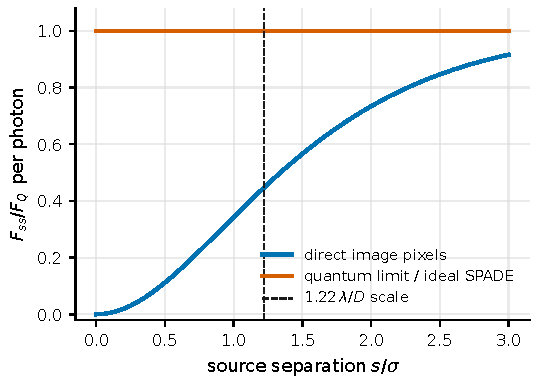
\includegraphics[width=0.82\linewidth]{figures/generated/chapter_08/ch08_rayleigh_information.pdf}
\caption{两颗等亮不相干高斯点源的间距信息。蓝线是由像面概率密度 \(p(x\mid s)\) 数值积分得到的直接成像 Fisher 信息（按量子极限归一化）；小间距时它以 \(s^2\) 掉向零，这就是 Rayleigh 诅咒。橙线是下一节的量子极限，即使 \(s\to0\) 也保持有限。竖虚线标出常用的 Rayleigh 角尺度。}
\label{fig:e12-rayleigh}
\end{figure}

\paragraph{检测问题不是估计问题}
\label{sec:e12-detection}

这里要划一条容易被忽略的界。上面整套 Fisher 语言默认我们\emph{已经接受}"天上是两颗等亮星"这个模型，只是不知道 \(s\)。这叫估计问题。另一类问题是"这到底是一颗星还是两颗星"——这叫\textbf{检测/模型选择}（detection / model selection）问题。两者不能混：检测问题里模型维数会变，而且 \(s=0\) 恰好落在参数空间的\emph{边界}上，常规的似然比近似（假设参数在内点、误差近高斯）在边界上未必成立，得靠模拟校准或贝叶斯证据来判。本章后面讲的所有"亚分辨增益"，都是在\emph{已接受双源模型}的前提下，把已经存在于光里的间距信息读得更干净——不是变魔术凭空造出一个源。

\paragraph{多参数：质心、亮度比、PSF 宽都会来抢信息}
\label{sec:e12-matrix}

真实观测里，间距 \(s\) 从来不是唯一未知量。质心位置 \(x_0\)、两颗星的亮度比 \(r\)、PSF 宽度 \(\sigma\)、背景 \(b\)……都得同时估。这时标量下界升级成\textbf{矩阵}版本。把所有参数排成向量 \(\bm\theta=(s,x_0,r,\sigma,b,\dots)\)，Fisher 信息成为一个矩阵：

\begin{equation}
  \mathrm{Cov}(\hat{\bm\theta})\ \succeq\ F^{-1},
  \qquad
  F_{\alpha\beta}=N_\gamma\int
  \frac{1}{p(x\mid\bm\theta)}
  \frac{\partial p}{\partial\theta_\alpha}
  \frac{\partial p}{\partial\theta_\beta}\,\mathrm{d}x.
  \label{eq:e12-fisher-matrix}
\end{equation}
\begin{formulaexplain}
\(F_{\alpha\beta}\)：Fisher 矩阵的第 \((\alpha,\beta)\) 元，比较参数 \(\theta_\alpha\)、\(\theta_\beta\) 对同一数据分布的影响。\(\mathrm{Cov}(\hat{\bm\theta})\succeq F^{-1}\)：协方差矩阵不小于 Fisher 矩阵的逆（矩阵不等式）。逆矩阵的对角元才是各参数的实际方差。
\end{formulaexplain}

关键在\emph{取逆}这一步。\(F\) 的非对角元记录参数间的\textbf{退化}（degeneracy）：如果两个参数对数据的影响"长得像"，它们的信息会互相纠缠，取逆后把误差放大。具体到亚分辨：未知质心会和间距混（把整幅图挪一点，很像把两颗星错开一点）；未知亮度比会在奇模式和偶模式之间重新分配信息；未知 PSF 宽度最阴险——它和双星间距都表现为"衍射斑变胖"（回想 \(s^2 h''\) 那一项！），两者几乎共线，若 \(\sigma\) 没被独立标定死，双星信号会被当成 PSF 变宽吸收掉。所以现实里报误差，不能只甩一个 \(1/\sqrt{F_{ss}}\)，得给出完整协方差、外加 PSF 标定误差、背景误差和模型误差。


\section{量子 Fisher 信息：把"测量方式"也放进优化}
\label{sec:e12-qfi}

到这里，一个尖锐的问题浮出来：直接成像的信息掉向零，那是\emph{光本身}就没带够信息，还是\emph{我们的测量方式}太笨？经典 Fisher 信息 \eqref{eq:e12-fisher-def} 是"先把测量方式定死（逐像素数光子），再问数据里有多少信息"。它把测量当成给定的。可量子力学允许的测量远不止"逐像素"一种——任意的正交投影、任意的干涉与模式分解都算数。

于是引入\textbf{量子 Fisher 信息}（quantum Fisher information，QFI）：在\emph{所有}量子力学允许的测量里取最优，同一束光原则上最多能读出多少参数信息。它是一切经典 Fisher 信息的上确界，\(F_{ss}\le F_{ss}^{Q}\)。QFI 只和光场的量子态怎么随参数变有关，和你选哪种探测器无关。

要写下这束光的态，我们借第 \ref{chap:e06} 章的弱热光结论。天体热光在每个相干时间模式里的平均光子数 \(\epsilon\ll1\)，所以密度矩阵近似是"真空 + 一点点单光子"：\(\rho\approx(1-\epsilon)|0\rangle\langle0|+\epsilon\,\rho_1\)。真空那一大块不点击、不带角信息——没有光子落下来，你无从知道两颗星隔多远。真正携带间距信息的，是那少数被探测到的\emph{单光子空间模式}。两颗等亮不相干点源的单光子部分是两个模式的等权混合：

\begin{equation}
  \rho_{1}(s)=\tfrac12\,\big|\psi_{+s/2}\big\rangle\big\langle\psi_{+s/2}\big|
             +\tfrac12\,\big|\psi_{-s/2}\big\rangle\big\langle\psi_{-s/2}\big|,
  \label{eq:e12-one-photon}
\end{equation}
\begin{formulaexplain}
\(\rho_1(s)\)：探测到一个光子时的空间模式密度矩阵。\(|\psi_{\pm s/2}\rangle\)：两颗星的光经过望远镜后，各自在像面形成的振幅模式（其模方就是平移了的 PSF）。不相干等亮 = 两个单光子态的等权概率混合。
\end{formulaexplain}

这里 \(|\psi_{\pm s/2}\rangle\) 是振幅 PSF，对高斯情形 \(\psi(x)\propto\exp[-x^2/(4\sigma^2)]\)（取模方 \(|\psi|^2\propto\exp[-x^2/(2\sigma^2)]=h\)，方差正好 \(\sigma^2\)）。

在正式抛结果之前，先让读者自己把那个关键的数落地。QFI 的大小，归根到底由振幅模式\emph{有多容易被平移区分}决定，而这由它的"动量方差"\(\Delta k^2=\int(\psi')^2\,\mathrm{d}x\) 定标——这一步用高斯就能手算。把归一化的 \(\psi(x)=(2\pi\sigma^2)^{-1/4}\exp[-x^2/(4\sigma^2)]\) 求导，\(\psi'(x)=-\dfrac{x}{2\sigma^2}\psi(x)\)，于是
\[
  \Delta k^2=\int\big[\psi'(x)\big]^2\,\mathrm{d}x
  =\frac{1}{4\sigma^4}\int x^2\,|\psi(x)|^2\,\mathrm{d}x
  =\frac{1}{4\sigma^4}\cdot\sigma^2
  =\frac{1}{4\sigma^2},
\]
用到了 \(\int|\psi|^2\,\mathrm{d}x=1\) 与 \(\int x^2|\psi|^2\,\mathrm{d}x=\sigma^2\)（同一条高斯二阶矩）。这个 \(1/(4\sigma^2)\) 正是下面单光子 QFI 里那个漂亮得出奇的数字的出处。在质心、亮度、PSF 宽都已知的理想条件下，对式 \eqref{eq:e12-one-photon} 那个 rank-2 混合态严格算 QFI，结果恰好是每光子 \(\Delta k^2\)：

\begin{equation}
  F_{ss}^{Q}=N_\gamma\,\frac{1}{4\sigma^{2}}.
  \label{eq:e12-qfi}
\end{equation}
\begin{formulaexplain}
\(F_{ss}^{Q}\)：所有允许测量能达到的间距信息\emph{上限}。\(\sigma\)：振幅模式对应的像面宽度。要害在于它\emph{不含 \(s\)}——\(s\to0\) 时它不消失，说明间距信息一直好端端待在光里，是直接成像把它漏掉了。
\end{formulaexplain}

需要对读者\emph{诚实}地交代一句：这里我们只算到了"定标尺度"\(\Delta k^2\)，而把 rank-2 混合态 QFI 的完整证明当作\textbf{已知结果引用}。它由 Helstrom 的量子估计理论奠基、经 Tsang 等人针对双源亚分辨给出显式值，我们在此直接采用 \citep{1969JSP.....1..231H,2016PhRvX...6c1033T}。混合态 QFI 要经由对称对数导数（symmetric logarithmic derivative，SLD）求解，严格推导超出本科范围，故不在此展开；但读者不必把 \eqref{eq:e12-qfi} 当"天上掉下来的"——\S\ref{sec:e12-spade} 会\emph{显式}造出 SPADE 这把尺，把经典 Fisher 信息一步步算到同一个 \(N_\gamma/(4\sigma^2)\)。这至少从下方确认了 \(F_{ss}^{Q}\ge N_\gamma/(4\sigma^2)\) 是可达的：既然存在一种真实测量能达到这个值，上限就不可能比它更低。

把 \eqref{eq:e12-qfi} 和直接成像的 \eqref{eq:e12-direct-fisher} 摆在一起看，反差刺眼：
\[
  \frac{F_{ss}^{\rm direct}}{F_{ss}^{Q}}
  =\frac{N_\gamma s^2/(8\sigma^4)}{N_\gamma/(4\sigma^2)}
  =\frac{s^2}{2\sigma^2}\ \xrightarrow{\,s\to0\,}\ 0.
\]
也就是说，在亚分辨区，直接成像用掉的信息占比以 \(s^2\) 趋零——绝大部分信息被白白丢掉了（图 \ref{fig:e12-rayleigh} 里蓝线掉下去、橙线不掉，画的就是这件事）。这不是望远镜绕过了衍射，而是"把测量方式也纳入优化"带来的裁决：信息在光里，就看你会不会读 \citep{1969JSP.....1..231H,2016PhRvX...6c1033T,2016OExpr..24.3684N}。下一节就造出那把"会读的尺"。


\section{SPADE：把小间距翻译成模式计数}
\label{sec:e12-spade}

QFI 只说"存在一种最优测量"，没说是哪一种。对高斯 PSF、等亮双源，那个最优（或接近最优）测量有个具体名字：\textbf{空间模式解调}（spatial-mode demultiplexing，SPADE）。它的想法一句话就能说清——\emph{别急着问光子落在哪个像素，先问它属于哪个正交空间模式，然后对每个模式分别数光子}。

对高斯 PSF，最自然的一组正交模式是 \textbf{Hermite--Gauss 模式}（Hermite--Gaussian modes），记作 \(u_0,u_1,u_2,\dots\)。它们其实是老熟人：第 \ref{chap:e04} 章的谐振子本征函数——一个高斯乘以 Hermite 多项式，\(u_0\) 是纯高斯、\(u_1\) 有一个节点、\(u_n\) 有 \(n\) 个节点。基模 \(u_0\) 恰好可以取成振幅 PSF 本身 \(\psi(x)\)。

\paragraph{为什么模式概率是 Poisson 分布}
\label{sec:e12-poisson}

现在算一颗星（位于 \(+s/2\)）的光落进各个模式的概率。它的振幅模式 \(\psi_{+s/2}(x)=\psi(x-s/2)\)，是把基模\emph{横向平移}了 \(d=s/2\)。这里可以借第 \ref{chap:e04} 章一个漂亮的对应：在谐振子语言里，把基态波函数在位置上平移一段 \(d\)，得到的正是一个\textbf{相干态}（coherent state）\(|\alpha\rangle\)，而相干态在数态（这里就是模式序号 \(n\)）上的占据概率是 Poisson 分布 \(|\langle n|\alpha\rangle|^2=e^{-|\alpha|^2}|\alpha|^{2n}/n!\)。位移 \(d\) 与 \(\alpha\) 的换算是 \(\alpha=d/(2x_{\rm zpf})\)，而对我们的模式，零点起伏尺度 \(x_{\rm zpf}=\sigma\)。所以

\[
  |\alpha|^{2}=\frac{d^{2}}{4\sigma^{2}}
  =\frac{(s/2)^{2}}{4\sigma^{2}}
  =\frac{s^{2}}{16\sigma^{2}}\ \equiv\ Q.
\]

另一颗星在 \(-s/2\)，位移是 \(-d\)，对应 \(\alpha\to-\alpha\)；但 Poisson 概率只依赖 \(|\alpha|^2\)，正负位移给出\emph{一模一样}的模式概率。于是两颗星的等权混合，其第 \(n\) 个模式的单光子点击概率就是

\begin{equation}
  p_{n}=e^{-Q}\,\frac{Q^{n}}{n!},
  \qquad
  Q=\frac{s^{2}}{16\sigma^{2}}.
  \label{eq:e12-spade-prob}
\end{equation}
\begin{formulaexplain}
\(p_n\)：光子落进第 \(n\) 个 Hermite--Gauss 模式的概率。\(Q\)：由间距和宽度拼出的无量纲"信号强度"，就是那个等效相干态的平均光子数。SPADE 把连续的间距，变成一列离散模式上的计数分布。
\end{formulaexplain}

这个 Poisson 形状用到了相干态的标准结果（第 \ref{chap:e06} 章）；如果你不想借谐振子，也可以直接算两个平移高斯与各 Hermite--Gauss 模式的重叠积分，会得到完全相同的 \(p_n\)。小 \(s\) 下展开：\(p_0=e^{-Q}\approx1-Q\)（几乎全部光子仍在基模），而
\[
  p_1=e^{-Q}Q\approx Q=\frac{s^{2}}{16\sigma^{2}},
\]
一小撮光漏进了第一阶（奇）模式 \(u_1\)。这一漏，正是间距信号本身。

\paragraph{第一阶模式的计数，与它为何能绕开诅咒}
\label{sec:e12-mode-fisher}

把概率乘以光子数，第一阶模式的期望计数是

\begin{equation}
  \langle n_1\rangle\simeq N_\gamma\,\frac{s^{2}}{16\sigma^{2}}.
  \label{eq:e12-n1}
\end{equation}
\begin{formulaexplain}
\(\langle n_1\rangle\)：第一阶模式里期望收到多少光子，等于总光子数乘以漏进该模式的概率 \(p_1\)。概率虽小，只要 \(N_\gamma\) 够大，就能攒成可测的计数。
\end{formulaexplain}

代真实数字。取 \(s=0.1\sigma\)（远在 Rayleigh 尺度之内），则
\[
  Q=\frac{(0.1)^2}{16}=\frac{0.01}{16}=6.25\times10^{-4},
  \qquad p_1\approx6.25\times10^{-4}.
\]
万分之六——听起来微不足道。可若这颗亮星给出 \(N_\gamma=10^{8}\) 个源光子（明亮恒星几秒到几分钟就能攒到），第一阶模式里理想情况下有 \(\langle n_1\rangle\approx6.3\times10^{4}\) 个光子，信噪比绰绰有余。反过来，若通量只有 \(N_\gamma=10^{5}\)，期望计数只剩约 63 个，这时暗计数、串扰和背景就会顶上来成为主要限制。

现在算模式测量的 Fisher 信息，看它怎么绕开诅咒。模式计数服从 Poisson/多项分布，其 Fisher 信息是各模式概率对 \(s\) 敏感度的加权和：

\begin{equation}
  F_{ss}^{\rm mode}
  =N_\gamma\sum_{n}\frac{1}{p_n}
  \left(\frac{\partial p_n}{\partial s}\right)^{2}.
  \label{eq:e12-mode-fisher}
\end{equation}
\begin{formulaexplain}
\(F_{ss}^{\rm mode}\)：模式计数携带的间距 Fisher 信息，求和跑遍所有空间模式。每一项是"概率随 \(s\) 的变化率"平方，除以该模式的计数噪声 \(p_n\)。
\end{formulaexplain}

小 \(s\) 下只有 \(n=1\) 项要紧。用 \(p_1\approx s^2/(16\sigma^2)\) 和它的导数 \(\partial p_1/\partial s\approx 2s/(16\sigma^2)=s/(8\sigma^2)\)，代进那一项：
\[
  \frac{1}{p_1}\left(\frac{\partial p_1}{\partial s}\right)^{2}
  =\frac{s^{2}/(64\sigma^{4})}{s^{2}/(16\sigma^{2})}
  =\frac{16\sigma^{2}}{64\sigma^{4}}
  =\frac{1}{4\sigma^{2}}.
\]
所以

\begin{equation}
  F_{ss}^{\rm mode}\ \xrightarrow{\,s\to0\,}\ N_\gamma\,\frac{1}{4\sigma^{2}}
  \;=\;F_{ss}^{Q}.
  \label{eq:e12-mode-saturates}
\end{equation}
\begin{formulaexplain}
在小间距极限，仅第一阶模式就把 Fisher 信息顶到量子上限 \eqref{eq:e12-qfi}。SPADE 因此\emph{饱和}了量子 Fisher 信息，把 Rayleigh 诅咒彻底绕开。
\end{formulaexplain}

看清这个"绕开"的机关：\(p_1\) 本身随 \(s^2\) 变小（信号弱），\(\partial p_1/\partial s\) 随 \(s\) 变小（斜率也弱），但在 Fisher 信息里是"斜率平方除以概率"，\(s^2/s^2\) 恰好\emph{约掉}，留下一个与 \(s\) 无关的有限值。直接成像栽在哪里？它把光子投到位置本征态，间距只留下 \(s^2\) 的形状展宽（\S\ref{sec:e12-curse}），分子分母的 \(s\) 幂次配不上，于是掉向零。SPADE 换了一组本征态（模式而非位置），刚好让幂次对上 \citep{2016PhRvX...6c1033T,2017NJPh...19b3054T}。图 \ref{fig:e12-spade-prob} 画出各模式概率随 \(s/\sigma\) 的增长，图 \ref{fig:e12-direct-vs-modes} 则把"像面几乎重合、模式计数已分开"这件事并排摆给你看。

\begin{figure}[tbp]
\centering
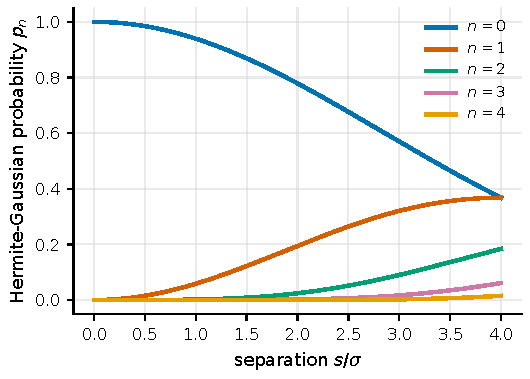
\includegraphics[width=0.82\linewidth]{figures/generated/chapter_08/ch08_spade_probabilities.pdf}
\caption{理想 Hermite--Gauss 模式排序的模式概率。横轴是间距 \(s/\sigma\)，纵轴是每个模式的单光子概率。小间距时 \(p_0\) 仍接近 1，而 \(p_1\) 及更高模式按 \(Q=s^2/(16\sigma^2)\) 的幂次抬头；间距信息正是由这些低概率模式的计数携带。}
\label{fig:e12-spade-prob}
\end{figure}

\begin{figure}[tbp]
\centering
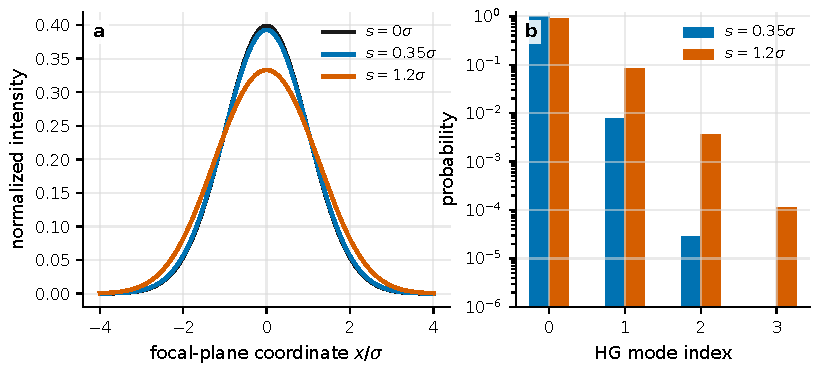
\includegraphics[width=0.92\linewidth]{figures/generated/chapter_08/ch08_direct_image_vs_modes.pdf}
\caption{同一双源模型在直接像面与模式输出中的两副面孔。左：\(s=0\)、\(0.35\sigma\)、\(1.2\sigma\) 的归一化像面强度，亚分辨时曲线差别只是极弱的展宽。右：\(s=0.35\sigma\) 与 \(1.2\sigma\) 时前四个 Hermite--Gauss 模式的概率，低阶非基模概率虽小，却把间距变成了清清楚楚的模式计数。}
\label{fig:e12-direct-vs-modes}
\end{figure}


\section{现实的限制：量子下界不是自动可达}
\label{sec:e12-reality}

漂亮的 \eqref{eq:e12-mode-saturates} 有一个大前提：模式基底精确对准了真实质心，而且模式排序器没有串扰、没有背景漏光。现实里这些都要打折扣，量子下界会被一层\textbf{系统误差平台}（systematic floor）顶住。

最致命的是\textbf{质心/指向误差}（centroid / pointing error）。SPADE 的第一阶模式 \(u_1\) 靠"整幅图相对模式中心的横向不对称"来装信号。可如果整幅图因为指向抖动、跟踪误差而整体偏了 \(\delta x\)，那这偏移\emph{本身}就会往 \(u_1\) 里灌光——而且机制和真信号一模一样。用上一节同样的相干态换算，整体偏移 \(\delta x\) 漏进第一阶模式的比例是
\[
  p_1^{\rm leak}\approx\frac{\delta x^{2}}{4\sigma^{2}},
\]
而真正的双星信号是 \(p_1^{\rm sig}\approx s^2/(16\sigma^2)\)。两者相等的条件是
\[
  \frac{\delta x^{2}}{4\sigma^{2}}=\frac{s^{2}}{16\sigma^{2}}
  \ \Longrightarrow\ \delta x=\frac{s}{2}.
\]
换句话说，只要质心标定误差达到间距的一半，赝信号就和真信号同量级——这时你测到的第一阶计数根本分不清是"两颗星"还是"望远镜没对准"。要测 \(s=0.1\sigma\) 的间距，就得把质心稳定和标定到远好于 \(0.05\sigma\)，这对指向、跟踪和标定是很硬的要求。

除此之外还有一串现实杀手：模式排序器的\textbf{串扰}（crosstalk）矩阵不稳定，会把 \(u_0\) 的强光漏一点到 \(u_1\)，淹没万分之几的信号；\textbf{背景光}若不具有和源相同的空间模式分布，会在各模式里铺一层底噪；Strehl 比不够、像差随时间漂、色散和偏振串扰都会污染模式响应矩阵。这些效应的共同特征是：它们\emph{不随 \(N_\gamma\) 下降}。统计误差按 \(1/\sqrt{N_\gamma}\) 一路降，可一旦撞上系统平台，再加光子也没用（图 \ref{fig:e12-crb} 里那条加了标定误差就压平的绿线，画的正是这件事）。所以"达到量子下界"从来不是自动的，实验上更常见的是较简单、较稳健的相位敏感测量（相位板、SLIVER、SPLICE 一类），它们缓和了直接成像的二次损失，但实际增益仍由可见度、串扰和对准误差说了算 \citep{2017PhRvL.118g0801T,2019NJPh...21i3010B,2018Optic...5.1177P}。

\begin{figure}[tbp]
\centering
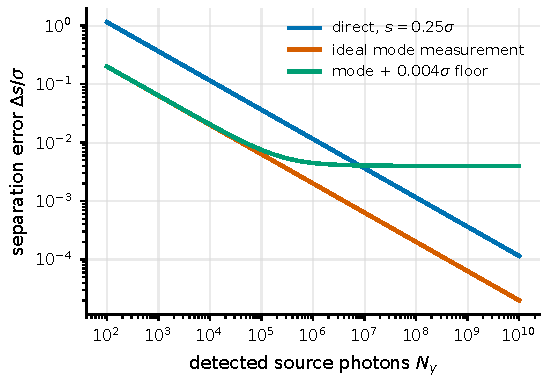
\includegraphics[width=0.82\linewidth]{figures/generated/chapter_08/ch08_cramer_rao_bound.pdf}
\caption{亚分辨双源的 Cramér--Rao 间距误差。横轴是探测源光子数 \(N_\gamma\)，纵轴是 \(\Delta s/\sigma\)。理想模式测量按 \(N_\gamma^{-1/2}\) 一路下降；直接成像因 Fisher 信息小得多，要更多光子才追平。绿线加入一小段模式匹配系统误差后出现平台——继续加光子也消不掉标定误差。}
\label{fig:e12-crb}
\end{figure}

还有一层更微妙的前提：源的\textbf{部分相干}（partial coherence）。上面全程假设两颗星互不相干（等权概率混合）。Larson 与 Saleh 指出，当源变得部分相干时，Rayleigh 诅咒可能\emph{重新出现}；Tsang 与 Nair 随后澄清，只要不是完全正相关的退化情形、并对弱热光做正确的 Fisher 计算，SPADE 仍能避免小间距信息彻底消失 \citep{2018Optic...5.1382L,2019Optic...6..400T}。天文学里尤其要分清两件事：源面上两块辐射区\emph{本身}独立不独立发光，与光传播到望远镜后、由 van Cittert--Zernike 定理（第 \ref{chap:e10} 章）造出的空间相干，是两码事。后者正是干涉测量要测的量，不能简单等同于源本身的相干发射。


\section{长基线的版本：强度干涉在傅里叶平面做同一件事}
\label{sec:e12-sii}

前面几节讲的是单孔径、或相干合束之后的空间模式测量。可"把分辨率当估计问题"这套思路，完全可以搬到公里级长基线阵列上去——只是这次舞台从像面换到\textbf{傅里叶平面}（Fourier plane）。第 \ref{chap:e10}、\ref{chap:e11} 章讲过：不同望远镜对之间的基线，采样天空亮度分布的不同空间频率；数据的约束来自\emph{可见度随基线怎么变}。这里的"亚分辨"，不再是从一个衍射斑里读两个峰，而是在长基线上量出源亮度分布的傅里叶模长。

强度干涉（intensity interferometry）不测一阶场相位，而测两台望远镜光强\emph{涨落}的相关。理想热光下，零延迟的二阶相关（第 \ref{chap:e10} 章的 Siegert/HBT 关系）给出

\begin{equation}
  g_{ij}^{(2)}(0)-1=\big|\gamma_{ij}\big|^{2},
  \label{eq:e12-hbt}
\end{equation}
\begin{formulaexplain}
\(g_{ij}^{(2)}(0)\)：望远镜 \(i,j\) 零时延二阶相关；减 1 得相对于"毫不相关"基线的超出。\(\gamma_{ij}\)：归一化复相干度，等于一阶可见度 \(V\)。强度涨落的同步程度，直接给出可见度模平方。
\end{formulaexplain}

于是观测量是一串基线/谱道/时段上的平方可见度：

\begin{equation}
  d_{k}=\big|V(u_k,v_k;\bm\theta)\big|^{2}+\eta_{k},
  \label{eq:e12-sii-data}
\end{equation}
\begin{formulaexplain}
\(d_k\)：第 \(k\) 个基线/时间/谱道上测到的平方可见度。\(V\)：源参数 \(\bm\theta\) 决定的模型可见度。\(\eta_k\)：噪声。角结构就写在 \(|V|^2\) 随基线的变化里。
\end{formulaexplain}

把同样的 Cramér--Rao 逻辑套上去。对参数 \(\theta_\alpha\)，强度干涉的 Fisher 矩阵是

\begin{equation}
  F_{\alpha\beta}^{\rm SII}
  =\sum_{k,l}
  \frac{\partial|V_k|^{2}}{\partial\theta_\alpha}\,
  C^{-1}_{kl}\,
  \frac{\partial|V_l|^{2}}{\partial\theta_\beta},
  \label{eq:e12-sii-fisher}
\end{equation}
\begin{formulaexplain}
\(F_{\alpha\beta}^{\rm SII}\)：强度干涉数据的 Fisher 矩阵。\(C^{-1}_{kl}\)：\(|V|^2\) 测量误差协方差的逆，给数据点加权。可见度模平方对参数越陡、误差越小，信息越多。
\end{formulaexplain}

其中 \(C_{kl}\) 是 \(|V|^2\) 测量误差的协方差，可用时间移位背景、空基线、隔夜重复观测或注入模拟来估。若各数据点误差近似独立，\(C\) 变对角，\eqref{eq:e12-sii-fisher} 就退化成"每点斜率平方除以方差再求和"——和单参数 \eqref{eq:e12-fisher-def} 是同一件事，只是求和取代了积分。要害在那个\emph{斜率} \(\partial|V|^2/\partial\theta\)：它告诉你哪条基线最有用。

代一个具体模型——均匀圆盘恒星。它的可见度是一阶 Bessel 函数（这来自圆盘亮度分布的傅里叶变换，第 \ref{chap:e10} 章推过）：

\begin{equation}
  V(x)=\frac{2J_1(x)}{x},
  \qquad x=\frac{\pi B\theta_\star}{\lambda},
  \label{eq:e12-uniform-disk}
\end{equation}
\begin{formulaexplain}
\(V(x)\)：均匀圆盘的可见度。\(J_1\)：一阶 Bessel 函数。\(B\)：投影基线（米）。\(\theta_\star\)：恒星角直径。基线通过无量纲的 \(x\) 扫描圆盘的傅里叶模长。
\end{formulaexplain}

\(V(x)\) 在 \(x=0\) 处为 1，随 \(x\) 增大先降到第一个零点（\(J_1\) 的第一个非平凡零点在 \(x\approx3.83\)，这是标准的 Bessel 零点），再翻出一串越来越弱的旁瓣。对角直径 \(\theta_\star\) 最有用的基线，落在 \(|V|^2\) 斜率 \(\partial|V|^2/\partial\theta_\star\) 最大的地方——通常在可见度快速下坠的那一段。短基线上 \(V\approx1\)、几乎不随 \(\theta_\star\) 变（平台上没斜率、没信息）；极长基线上信号又掉进旁瓣、容易被系统误差压住。所以"基线不是越长越好"，而是要\emph{挑在斜率大处}。图 \ref{fig:e12-sii-fisher} 把这条设计原则画得很直白。

\begin{figure}[tbp]
\centering
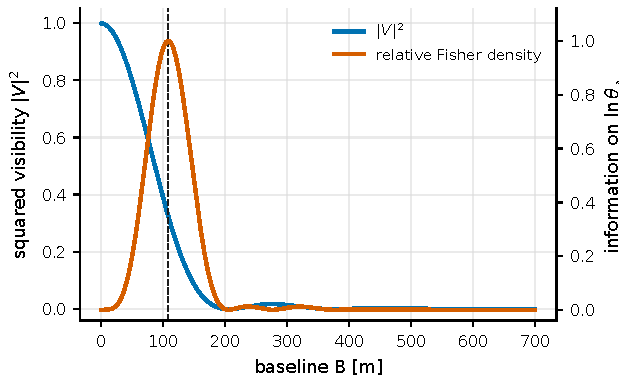
\includegraphics[width=0.82\linewidth]{figures/generated/chapter_08/ch08_visibility_fisher_design.pdf}
\caption{强度干涉里基线选择与参数信息的关系。蓝线是 \(\lambda=450~\mathrm{nm}\)、\(\theta_\star=0.55~\mathrm{mas}\) 均匀圆盘的平方可见度；橙线是按 \(\partial|V|^2/\partial\ln\theta_\star\) 算出并归一化的 Fisher 权重。最有用的基线落在可见度快速下降处；单纯拉长或缩短基线都不会自动增加角直径信息。}
\label{fig:e12-sii-fisher}
\end{figure}

强度干涉的代价是\textbf{相位缺失}：\(|V|^2\) 丢掉了 \(V\) 的相位，因此对整体平移不敏感，还会带来镜像与中心对称退化——二元星的取向、亮斑位置、非对称盘面往往要靠地球自转带来的 \(uv\) 覆盖、多波长、先验模型或三阶相关来缓解。它换来的好处极大：对大气相位扰动几乎免疫。因为它只比较两路\emph{强度}抖动同不同步，望远镜之间只需电子连接、把信号在时间上对齐到探测响应的一小部分即可，不必维持光学相干（第 \ref{chap:e10} 章算过，纳秒级电子时间对应几十厘米的光程容差，大气 piston 那点纳米级抖动完全落在容差里）。正因如此，那些光学像质远不及专业干涉仪、却坐拥大收集面积和长基线的大气 Cherenkov 望远镜阵列，反而成了理想的强度干涉阵 \citep{1956Natur.177...27B,1974MNRAS.167..121H,2020NatAs...4.1164A,2024MNRAS.529.4387A}。

\paragraph{两条工程路线的分工}
\label{sec:e12-two-roads}

把两种"亚分辨估计"并排看，它们的工程瓶颈正好相反，因此适用对象也不同：

\begin{itemize}
  \item \textbf{SPADE / 空间模式测量}（单孔径或相干合束）：要求\emph{稳定的波前}。目标光要耦进光纤模式、集成光学芯片或自由空间模式排序器，自适应光学把入射光尽量压进少数可控模式。它的敌人是 Strehl 比、非共路像差、质心抖动和模式串扰。适合读出两颗近星的角间距、恒星的低阶形状矩这类少参数问题。
  \item \textbf{强度干涉}（长基线阵列）：干脆\emph{接受}大气把相位随机化，用大收集面积和长基线去换 \(|V|^2\) 信息。它的敌人是光子率低、电子带宽、背景、时间同步和系统协方差。适合亮热星、快速自转星、双星和角直径测量。
\end{itemize}

无论走哪条路，一套能拿出去发表的亚分辨估计，都得同时交代四本账：\emph{光子预算}（星等、谱带、总效率、曝光 \(\to\) 有效 \(N_\gamma\)）、\emph{角尺度}（\(\lambda/D\)、PSF 宽 \(\sigma_\theta\)、候选间距 \(s\) 或角直径 \(\theta_\star\)）、\emph{测量矩阵}（像素响应、模式串扰、或 \(|V|^2\) 协方差）、\emph{模型边界与误差拆分}（等亮双源、未知亮度比、有限圆盘、部分相干、背景星怎样改写 Fisher 矩阵）。最后检查一条判据就够诊断：统计误差还在按 \(N_\gamma^{-1/2}\) 下降吗？若不再降，八成是对准、PSF、背景、相关器或模型误差撞上了平台。把这些边界放进最终推断，常用贝叶斯采样与证据比较——直接成像、模式计数、强度干涉数据可以共享同一个参数向量、联合似然相乘；已知轨道、颜色、光谱型、距离等先验会直接改变可识别的参数空间 \citep{2009MNRAS.398.1601F,2013PASP..125..306F}。


\section{本章要点}
\label{sec:e12-summary}

\begin{itemize}
  \item \textbf{分辨率是估计问题，不是成像判据。} Rayleigh 判据 \(\theta_{\rm R}=1.22\lambda/D\) 只问"像面能不能分成两峰"；真正该问的是"给定 \(N_\gamma\) 个光子，间距 \(s\) 能估到多准"，答案由 Fisher 信息与 Cramér--Rao 下界 \(\mathrm{Var}(\hat s)\ge1/F_{ss}\) 给出。
  \item \textbf{小间距先变胖、不先分家。} 把两个平移 PSF 泰勒展开，一阶项相消，\(p(x\mid s)=h+\tfrac{s^2}{8}h''+\mathcal O(s^4)\)。间距最低阶通过 \(h''\) 表现为二阶展宽，直接成像 Fisher 信息 \(F_{ss}^{\rm direct}\simeq N_\gamma s^2/(8\sigma^4)\to0\)——这就是 Rayleigh 诅咒。
  \item \textbf{信息没离开光。} 量子 Fisher 信息把"逐像素"换成"所有允许测量"，对弱热光单光子态得 \(F_{ss}^{Q}=N_\gamma/(4\sigma^2)\)，\(s\to0\) 时不消失。诅咒是测量方式的病，不是光的病。
  \item \textbf{SPADE 饱和量子极限。} 先投到 Hermite--Gauss 模式再计数，模式概率是 Poisson 分布 \(p_n=e^{-Q}Q^n/n!\)，\(Q=s^2/(16\sigma^2)\)。第一阶模式里 \(p_1\propto s^2\)、\(\partial p_1/\partial s\propto s\)，二者在 Fisher 信息中相除留下有限极限 \(N_\gamma/(4\sigma^2)\)，绕开诅咒。
  \item \textbf{下界不是自动可达。} 质心误差 \(\delta x\) 漏进第一阶模式的量 \(\delta x^2/(4\sigma^2)\)，当 \(\delta x\sim s/2\) 时就与信号 \(s^2/(16\sigma^2)\) 同量级；串扰、背景模式、部分相干都会制造不随 \(N_\gamma\) 下降的系统平台。
  \item \textbf{长基线是同一件事的傅里叶版。} 强度干涉在傅里叶平面估参数，\(F^{\rm SII}_{\alpha\beta}=\sum\partial|V|^2/\partial\theta\,C^{-1}\,\partial|V|^2/\partial\theta\)，最有用的基线在 \(|V|^2\) 斜率大处。它丢相位、免大气，与 SPADE 的"稳波前"路线互补。
\end{itemize}

\medskip
\noindent\textbf{想一想。}
\begin{enumerate}
  \item 若把两颗星的\emph{亮度比}也设为未知参数，第一阶（奇）模式和基模（偶模式）各自还剩多少间距信息？为什么"未知亮度比"这个退化，会削弱奇模式的贡献？
  \item 直接成像的 \(F_{ss}^{\rm direct}\propto s^2\) 是在\emph{高斯} PSF 下推的。换成有真实旁瓣的 Airy PSF，二阶展宽这一步会不会改变？Rayleigh 诅咒是高斯的特产，还是更普遍的现象？
  \item 强度干涉丢掉了相位，SPADE 保留了模式的相对相位信息。对"测两颗近星的\emph{取向}"这个任务，哪一种更有优势？把它翻译成 \eqref{eq:e12-sii-fisher} 里的退化来说明。
\end{enumerate}


% ============================================================
\part{仪器、事件表与观测设计}
\chapter{探测器、时钟与事件表}
\label{chap:e13}

\begin{chapteropening}
第 \ref{chap:e07} 章告诉我们，探测的本质是"吸收一个光子、吐出一次电脉冲"；第 \ref{chap:e08} 章又告诉我们，藏在事件流里的相关峰可以小到 \(10^{-6}\)，而且会被探测器有限的时间响应卷积展宽、稀释。可这两章都还停在"理想探测器"的层面。真实的望远镜没有理想探测器：光子撞上光阴极只有一定概率变成电子；每个电脉冲到来的时刻都带着几十皮秒到几纳秒的随机抖动；探测器每响一次就要"喘口气"，在这段死时间里对新光子视而不见；两台相距百米的望远镜，各自的时钟还得对齐到皮秒。本章要回答一个非常"硬件"的问题：一个光子，究竟经过哪些环节，才变成事件表里那一行\emph{带时间戳的记录}？我们会把量子效率、时间抖动、死时间与堆积、afterpulsing、时钟同步这几件事逐一拆开，把每一个公式从头推到尾，最后落到"事件表该存哪些字段"这张最实用的清单上。
\end{chapteropening}

\section{从光子到一行带时间戳的事件}
\label{sec:e13-from-photon-to-event}

先把上一阶段的结论接住。第 \ref{chap:e07} 章把"探测"讲成了一个概率事件：一个能量为 \(h\nu\) 的光子打到探测器上，有一定概率被吸收并触发一次可记录的电脉冲。第 \ref{chap:e08} 章把这些电脉冲排成一串带时间戳的"点击"，并教我们从中读出 \(g^{(2)}(\tau)\)。但那里的探测器是"透明"的——光子进去，事件出来，中间不损耗、不延迟、不饱和。真实器件恰恰相反：它在光子和事件之间设了好几道关卡，每一道关卡都会改写事件率、时间戳或峰形。本章就是要把这几道关卡一一打开。

关键的数据结构叫\textbf{事件表}（event list）。它和普通的光变曲线（light curve）有本质区别。光变曲线是"把一段曝光里的光子数累加到一个时间 bin 上"——一旦累加，谁在什么时刻来的、来自哪个望远镜、哪个波长、哪个偏振，全都糊成了一个数。事件表则相反，它\emph{逐个光子}保留信息：到达时刻、望远镜编号、探测器通道、波长通道、偏振通道、权重、质量标记。为什么值得这么"啰嗦"地存？因为二阶相关、脉冲星折叠、快速遮掩这些测量，信号恰恰藏在"哪两个光子几乎同时到达"这种联合信息里；只要过早地按时间 bin 累加，待测的相关峰就被抹掉了，事后再也补不回来。Iqueye 就是这么设计的：它把每个光子都打上时间标签保存，事后再离线选择从 24.41 ps 到分钟级的任意时间 bin；对 \(\zeta\) Ori 的一次观测就产生了约 \(2\times10^{10}\) 个光子事件、约 78 GB 数据 \citep{2009A&A...508..531N,2019CoSka..49...85Z}。可见事件表不是可有可无的辅助文件，而是真实望远镜的主要数据产品。

把一行原始事件写下来，它长这样：
\begin{equation}
  \mathcal{E}^{\rm raw}_q =
  \big(n_q,\ a_q,\ d_q,\ c_q,\ p_q,\ f_q,\ w_q\big),
  \qquad
  t^{\rm raw}_q=t_0+n_q\,\delta t+\epsilon_{\rm roll}.
  \label{eq:e13-raw-event}
\end{equation}
\begin{formulaexplain}
\(\mathcal E_q^{\rm raw}\) 是第 \(q\) 个原始事件；\(n_q\) 是时钟计数（tick），\(\delta t\) 是一个 tick 的时长，\(t_0\) 是记录段起点，\(\epsilon_{\rm roll}\) 处理计数器溢出。它把一次电子记录翻译成最早的事件时刻。
\end{formulaexplain}
逐个符号落实。下标 \(q\) 编号第 \(q\) 个事件。\(n_q\) 是电子计数器读到的整数 tick 数（无量纲）；\(\delta t\) 是一个 tick 对应的时间（单位秒），现代时间数字转换器（time-to-digital converter, TDC）的 \(\delta t\) 常在 \(10^{-11}\)--\(10^{-10}\,{\rm s}\) 量级，商用多通道 TCSPC 系统基本时间分辨率可到 80 ps，Iqueye 的量化步长是 24.41 ps \citep{2009A&A...508..531N,2020RScI...91a3108W}。\(t_0\) 是记录段的起始时刻（秒），\(\epsilon_{\rm roll}\) 处理计数器满量程后回绕（rollover）或分段。后面几个整数都是"标签"：\(a_q\) 是望远镜或站点编号，\(d_q\) 是探测器编号，\(c_q\) 是波长通道或滤光片编号，\(p_q\) 是偏振通道，\(f_q\) 是质量标记，\(w_q\) 是事件权重。溢出、丢包、饱和、云、指向异常、电子学异常都应该写进 \(f_q\)——否则日后相关函数里冒出一个诡异的峰，你将无从追溯它是天体还是故障。

\begin{figure}[tbp]
\centering
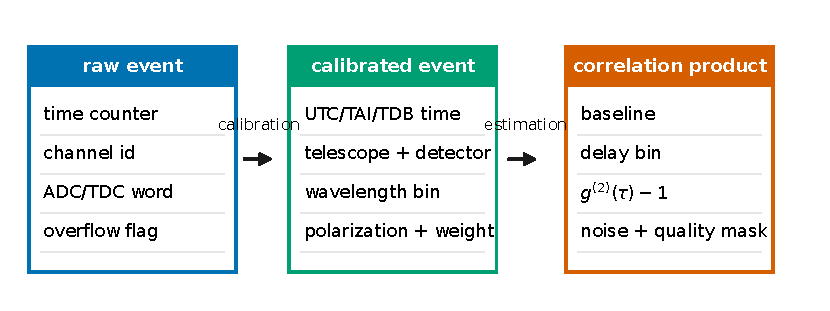
\includegraphics[width=0.96\linewidth]{figures/generated/chapter_06/ch06_event_table_schema.pdf}
\caption{事件数据从原始电子记录流向标定事件表，再流向相关函数产品。原始层保存计数器时间、通道编号和溢出标记；标定层把时间转换到统一时间尺度，并加入望远镜、波长、偏振和权重；相关产品层才记录基线、延迟 bin、相关幅度与噪声估计。若在第一层就只保存光变曲线，后面的时钟、波长和偏振选择都将无法重新执行。}
\label{fig:e13-event-table-schema}
\end{figure}

本章的路线也就清楚了：先看光子怎样以概率 \(\eta\) 变成电子事件（\ref{sec:e13-detectors} 节），再看每个事件时刻带着多大抖动、如何把相关峰卷宽（\ref{sec:e13-jitter} 节），接着看探测器"喘气"造成的死时间与堆积如何让记录率饱和（\ref{sec:e13-deadtime} 节）、afterpulsing 如何伪造短延迟相关（\ref{sec:e13-afterpulse} 节），然后把两台望远镜的时钟对齐到皮秒（\ref{sec:e13-clock} 节），最后落到事件表字段清单（\ref{sec:e13-schema} 节）和谱分辨与相干时间的权衡（\ref{sec:e13-spectral} 节）。

\section{探测器：量子效率把光子变成电子事件}
\label{sec:e13-detectors}

探测器的第一项、也是最基本的作用，是决定"有多少入射光子真的变成了电子事件"。这一步的核心参数叫\textbf{量子效率}（quantum efficiency）\(\eta\)：一个到达感光面的光子，被吸收并触发一次可计数脉冲的概率。它无量纲，取值在 0 和 1 之间，而且强烈依赖波长。把整条光路的效率乘起来，一个通道的平均探测率是
\begin{equation}
  R_{\rm det}
  =
  A_{\rm eff}
  \int_{\lambda_1}^{\lambda_2}
  F_\lambda(\lambda)\,
  T_{\rm opt}(\lambda)\,
  \eta(\lambda)\,
  d\lambda
  \;+\;R_{\rm sky}+R_{\rm dark}.
  \label{eq:e13-detected-rate}
\end{equation}
\begin{formulaexplain}
\(R_{\rm det}\) 是探测计数率；\(A_{\rm eff}\) 是有效集光面积；\(F_\lambda\)、\(T_{\rm opt}\)、\(\eta\) 分别是源光子谱通量、光路透过率和量子效率；\(R_{\rm sky},R_{\rm dark}\) 是天光背景与暗计数。它是一份"事件率预算"。
\end{formulaexplain}
逐项交代单位与量级。\(A_{\rm eff}\) 是有效集光面积（\({\rm m}^2\)），对大气 Cherenkov 望远镜可达几十到上百 \({\rm m}^2\)。\(F_\lambda\) 是源的光子谱通量密度（\({\rm photons\,s^{-1}\,m^{-2}\,nm^{-1}}\)）。\(T_{\rm opt}\) 是镜面、滤光片、光纤、准直器、窗口的总透过率（无量纲，通常远小于 1）。\(\eta(\lambda)\) 是量子效率。\(R_{\rm sky}\) 是天光和杂散光的计数率，\(R_{\rm dark}\) 是探测器在完全无光时也会自发产生的暗计数率（两者单位都是 \({\rm s}^{-1}\)）。式子的结构很直白：源贡献是"面积 × 谱通量 × 透过率 × 效率"在带宽内的积分，再加上两项与源无关的背景。强度干涉的信噪比，最终就由"被背景稀释后的恒星光子率与强度起伏"共同决定；MAGIC-SII 直接用 PMT 直流电流估计光子通量、用背景像素修正夜天光，VERITAS-SII 用 off-source 测量估计背景再把相关幅度按恒星光占比修正 \citep{2020NatAs...4.1164A,2024MNRAS.529.4387A}。

不同任务要用不同探测器，它们在"效率、时间分辨、面积、暗计数"之间各有取舍。把常见的几类摆在一起看：

\begin{itemize}
  \item \textbf{光电倍增管（PMT，photomultiplier tube）}：光子打在光阴极上打出光电子，经过一串打拿极（dynode）逐级倍增，增益可达 \(10^6\) 量级。它面积大、增益高、脉冲窄（ns 级），和 Cherenkov 望远镜的高速电子链天然匹配；蓝光量子效率常在 \(20\%\)--\(40\%\)，VERITAS-SII 在 416 nm 使用的 PMT 量子效率约 \(30\%\) \citep{2020NatAs...4.1164A,2024MNRAS.529.4387A}。它是当代地面强度干涉的主力探测器。
  \item \textbf{雪崩光电二极管（APD，avalanche photodiode）}：半导体器件，靠反向偏压下的雪崩倍增放大信号。工作在偏压低于击穿电压的\emph{线性模式}时，输出正比于入射光强，增益适中、噪声较低，适合中等到较强光通量，但通常不做单光子计数。
  \item \textbf{单光子雪崩二极管（SPAD，single-photon avalanche diode）}：把 APD 偏置到\emph{击穿电压以上}（盖革模式，Geiger mode），一个光电子就能触发一次自持雪崩，产生一个"有/无"的数字脉冲。可见光量子效率可达 \(50\%\)--\(60\%\)，单光子时间分辨率约 30--50 ps，暗计数常见 10--100 \({\rm s}^{-1}\)；代价是感光面积小、死时间较长，而且雪崩后会有 afterpulsing 污染短延迟相关（下文详述）\citep{1996ApOpt..35.1956C,2009JMOp...56..261B,2009A&A...508..531N,2015SPIE.9504E..0CZ}。
  \item \textbf{硅光电倍增管（SiPM，silicon photomultiplier）}：把成百上千个微小 SPAD 单元（microcell）并联成一块面阵，每个单元只报"有/无"，把它们的输出相加就得到近似正比于光子数的信号。它兼顾了单光子灵敏度与较大的有效面积，供电低、不怕强光损伤，已进入新一代 Cherenkov 相机；代价是单元间存在光学串扰（optical crosstalk），暗计数率也比单个 SPAD 高。
  \item \textbf{超导纳米线单光子探测器（SNSPD，superconducting nanowire single-photon detector）}：把一根偏置到临界电流附近的超导纳米线冷却到几开尔文，一个光子被吸收就足以破坏局部超导态、产生一个可记录的电压脉冲。它同时做到高量子效率（可达 \(90\%\) 以上）、极低暗计数（可低至 \({\rm s}^{-1}\) 量级以下）和皮秒级时间抖动，是当前计时与暗计数综合性能最强的单光子探测器；代价是需要低温制冷系统、感光面积小。
  \item \textbf{能量分辨型探测器（如 MKID，microwave kinetic inductance detector，微波动电感探测器）}：这类超导器件在吸收一个光子后，其超导动电感随入射光子能量而变，因而能\emph{直接读出每个光子的波长}，天生自带光谱通道。代价是时间分辨率通常只到微秒量级、死时间长，且同样需要低温系统——它用时间分辨换取了能量（波长）分辨。
\end{itemize}

\begin{figure}[tbp]
\centering
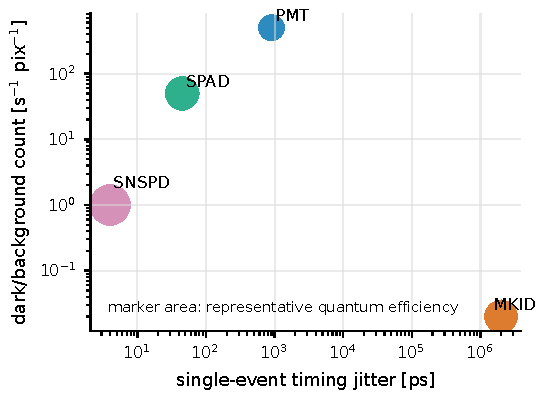
\includegraphics[width=0.72\linewidth]{figures/generated/chapter_06/ch06_detector_trade_space.pdf}
\caption{几类单光子探测技术的典型工作区域。横轴是单事件时间抖动，纵轴是每像素暗计数或背景计数的代表值，点面积表示代表性量子效率。PMT 适合大口径、高通量和 ns 级强度干涉；SPAD 给出几十皮秒计时但受面积与死时间限制；超导器件在低暗计数与皮秒计时上最强，但需要低温系统；能量分辨型探测器则牺牲时间分辨换取每个光子的波长信息。}
\label{fig:e13-detector-trade-space}
\end{figure}

一句话把这一节收住：\(\eta\) 决定\emph{有多少}光子变成事件，进而决定信噪比里的"信号"；而"事件何时到、探测器多久能再响一次"这些时间性质，决定了事件表里的相关结构还忠不忠实于入射光场——这正是接下来三节要拆的东西。

\section{时间抖动：相关峰为什么会被展宽}
\label{sec:e13-jitter}

第 \ref{chap:e08} 章已经预告：探测器有限的时间响应会把窄相关峰卷积展宽、峰高稀释。现在我们把这件事讲透。问题的根源是\textbf{时间抖动}（timing jitter）：即便同一个光子在同一时刻到达，探测器输出脉冲被判定为"事件"的那个时刻，每次都略有不同，是一个随机量。对 SPAD 约几十皮秒，对 PMT 加电子链可到 ns 级。把这种随机延迟写成一个响应函数 \(h(t)\)（归一化的概率分布，描述"真实到达时刻 0 对应的记录时刻分布"），那么观测到的事件时间就是真实时间与 \(h\) 的卷积。

对二阶相关，两个通道各有响应 \(h_1(t)\)、\(h_2(t)\)，观测到的相关超额是天体真实相关与合成响应的卷积：
\begin{equation}
  C^{\rm obs}_{12}(\tau)
  =
  \int C^{\rm sky}_{12}(\tau')\,
  h_{12}(\tau-\tau')\,d\tau',
  \qquad
  h_{12}=h_1*h_2.
  \label{eq:e13-response-convolution}
\end{equation}
\begin{formulaexplain}
\(C^{\rm sky}_{12}\) 是天体真实相关，\(C^{\rm obs}_{12}\) 是观测结果；\(h_1,h_2\) 是两通道时间响应，\(h_{12}\) 是它们的卷积。仪器把窄相关峰"抹宽"。
\end{formulaexplain}
这里 \(C_{12}=g^{(2)}_{12}-1\)（无量纲），\(\tau,\tau'\) 单位是秒，\(*\) 是卷积。物理图像很直白：真实相关峰无限窄也没用，因为你根本不知道每个光子的\emph{准确}到达时刻，只知道它落在一个宽约 \(\sigma\) 的模糊窗口里；两路模糊叠加，观测峰就被展宽到 \(h_{12}\) 的宽度。

要把"展宽多少"算清楚，用一个非常好用的近似：把每个响应都当作高斯。这里要点名一个标准结果——\emph{两个高斯函数的卷积仍是高斯，且方差相加}。设 \(h_1\) 是宽度（方差）\(\sigma_1^2\) 的高斯、\(h_2\) 是 \(\sigma_2^2\) 的高斯，则
\[
  h_{12}=h_1*h_2 \;\Longrightarrow\; \sigma_{12}^2=\sigma_1^2+\sigma_2^2 .
\]
把源自身的宽度、光路展宽、时钟残差也一并算进来，各项若彼此独立，方差就直接相加（这叫"按方差相加"，是独立高斯展宽叠加的普遍规则）：
\begin{equation}
  \sigma_{\rm obs}^2
  \simeq
  \sigma_{\rm sky}^2+\sigma_1^2+\sigma_2^2+\sigma_{\rm opt}^2+\sigma_{\rm clk}^2 .
  \label{eq:e13-jitter-budget}
\end{equation}
\begin{formulaexplain}
\(\sigma_{\rm obs}\) 是观测峰宽；\(\sigma_{\rm sky}\) 是源自身宽度，\(\sigma_1,\sigma_2\) 是两探测器抖动，\(\sigma_{\rm opt}\) 是光路展宽，\(\sigma_{\rm clk}\) 是时钟残差。独立高斯展宽按方差相加。
\end{formulaexplain}
每一项都是 rms 时间宽度（秒）。\(\sigma_{\rm sky}\) 是光源的相干时间或脉冲宽度，\(\sigma_1,\sigma_2\) 是探测器与电子通道的抖动，\(\sigma_{\rm opt}\) 是镜面等时性误差（比如 Davies--Cotton 镜面不同格子的光程差），\(\sigma_{\rm clk}\) 是两站时钟对齐后的残差。这里有个重要的"数量级落地"：可见光宽带的相干时间 \(\tau_c\) 短到皮秒（第 \ref{chap:e02} 章），比 ns 级的 \(\sigma_1,\sigma_2\) 小了三个数量级，于是式 \eqref{eq:e13-jitter-budget} 里 \(\sigma_{\rm sky}\) 项几乎可以忽略——\emph{观测峰宽几乎完全由仪器决定}。VERITAS 的镜面加 PMT 脉冲宽度使强度相关峰可用 \(\sigma_\tau\simeq4\,{\rm ns}\) 的高斯描述，MAGIC-SII 的相关峰高斯宽度约 \(2.2\,{\rm ns}\) \citep{2020NatAs...4.1164A,2024MNRAS.529.4387A}。

这带来一个关键后果：\emph{峰宽变了，峰高也跟着变}。因为相关峰下的"面积"（真实相关的总强度）在卷积中近似守恒，把它摊到更宽的峰上，峰高就按展宽因子被稀释。若真实峰宽 \(\sigma_{\rm sky}\ll\sigma_{\rm obs}\)，观测峰高相对真实峰高大约被压低了一个 \(\sigma_{\rm sky}/\sigma_{\rm obs}\) 的因子。这就是第 \ref{chap:e08} 章说"相关峰会被时间响应稀释"的定量来源，也解释了为什么强度干涉要拼命追求高电子带宽和稳定的响应函数——响应越窄，峰高稀释越少，越容易把 \(10^{-6}\) 量级的峰从噪声里挑出来。

\begin{figure}[tbp]
\centering
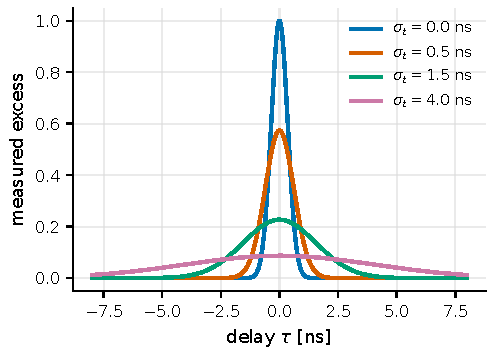
\includegraphics[width=0.72\linewidth]{figures/generated/chapter_06/ch06_detector_timing_response.pdf}
\caption{有限时间响应把窄相关峰展宽并降低峰高。曲线保持峰面积近似不变，只改变 rms 抖动 \(\sigma_t\)。当真实相干时间远短于 ns 级电子响应时，峰宽主要由仪器决定，峰高按展宽因子被稀释；这正是强度干涉需要高电子带宽和稳定响应函数的原因。}
\label{fig:e13-detector-timing-response}
\end{figure}

\section{死时间与堆积：记录率为什么会饱和}
\label{sec:e13-deadtime}

抖动改变的是每个事件的\emph{时刻}；死时间改变的是\emph{有多少事件}能被记下来。\textbf{死时间}（dead time）\(\tau_d\) 是探测器响一次之后"喘气"的一段时间，在此期间它对新光子视而不见。当光子来得又快又密，死时间就会吃掉大量事件，让记录率 \(r_{\rm rec}\) 明显低于真实入射率 \(r\)——这叫\textbf{堆积}（pile-up）造成的计数损失。这里有一个微妙但重要的分岔：死时间到底会不会被"死时间里到来的光子"再次刷新？两种回答给出两种模型，务必分清。

\paragraph{非麻痹型：死时间不被刷新}

先看\textbf{非麻痹型}（non-paralyzable）。它假设：探测器记下一个事件后死 \(\tau_d\)，这段时间里来的光子一律丢弃，\emph{但不会延长}死时间；\(\tau_d\) 一到，探测器立刻复活等下一个。推导用一个"活时间账本"的办法，零跳步地做出来。

设总观测时长为 \(T\)，真实入射率为 \(r\)（\({\rm s}^{-1}\)），记录到的事件总数为 \(M\)。每记录一个事件就死 \(\tau_d\)，所以总死时间是 \(M\tau_d\)，于是探测器真正"活着、能响应"的时间是
\[
  T_{\rm live}=T-M\tau_d .
\]
非麻痹型的关键是：只有在活时间里到来的光子才会被记录，而在活时间里，光子以真实率 \(r\) 泊松地到来，所以
\[
  M=r\,T_{\rm live}=r\,(T-M\tau_d).
\]
把含 \(M\) 的项归拢：
\[
  M=rT-rM\tau_d \;\Longrightarrow\; M+rM\tau_d=rT \;\Longrightarrow\; M(1+r\tau_d)=rT .
\]
两边除以 \(T\)，记 \(r_{\rm rec}=M/T\)，就得到记录率：
\begin{equation}
  r_{\rm rec}=\frac{r}{1+r\tau_d}.
  \label{eq:e13-nonparalyzable}
\end{equation}
\begin{formulaexplain}
\(r\) 是真实入射率，\(r_{\rm rec}\) 是记录率，\(\tau_d\) 是死时间。非麻痹型里死时间内的光子被丢弃、但不延长恢复窗口，所以 \(r_{\rm rec}\) 随 \(r\) 单调上升并饱和到 \(1/\tau_d\)。
\end{formulaexplain}
读一下这条式子的极限。低通量 \(r\tau_d\ll1\) 时分母趋近 1，\(r_{\rm rec}\approx r(1-r\tau_d)\)，损失很小；高通量 \(r\tau_d\gg1\) 时 \(r_{\rm rec}\to 1/\tau_d\)——记录率\emph{饱和}到一个上限，探测器每 \(\tau_d\) 顶多报一个事件，再多的光子也挤不进来，但绝不会倒退。

\paragraph{麻痹型：每个光子都刷新死时间}

再看\textbf{麻痹型}（paralyzable）。它假设：死时间内到来的每一个新光子，虽然\emph{不被记录}，却会\emph{重新触发}一段 \(\tau_d\) 的死时间。于是只有当一个光子到来时、它前面已经\emph{空了至少 \(\tau_d\)}没有任何光子，这个光子才会被记录。

推导要用泊松过程的一条标准结果：对速率为 \(r\) 的泊松过程，相邻两个光子之间的时间间隔服从指数分布，\emph{间隔超过 \(\tau_d\) 的概率是 \(e^{-r\tau_d}\)}。（这就是"在长度 \(\tau_d\) 的窗口里一个光子都没有"的概率，等于泊松分布取 0 个：\(P(0)=e^{-r\tau_d}\)。）一个到来的光子能被记录，当且仅当它之前的那段空窗大于 \(\tau_d\)。所有光子以率 \(r\) 到来，其中"前置空窗 \(>\tau_d\)"的那一部分才算数，所以记录率是
\[
  r_{\rm rec}=r\times P(\text{前置间隔}>\tau_d)=r\,e^{-r\tau_d}.
\]
写成编号式子：
\begin{equation}
  r_{\rm rec}=r\,e^{-r\tau_d}.
  \label{eq:e13-paralyzable}
\end{equation}
\begin{formulaexplain}
同样是死时间模型，但每个到来的光子都会刷新恢复窗口。因此 \(r_{\rm rec}\) 在 \(r\tau_d=1\) 处达到最大，之后随 \(r\) 增大反而\emph{下降}——高通量下探测器几乎一直被刷新、报不出事件。
\end{formulaexplain}
读极限：低通量 \(r\tau_d\ll1\) 时 \(e^{-r\tau_d}\approx1-r\tau_d\)，\(r_{\rm rec}\approx r(1-r\tau_d)\)——和非麻痹型在低通量下\emph{完全一致}，这也是为什么弱光下两种模型很难区分。但高通量截然不同：把 \(r_{\rm rec}=re^{-r\tau_d}\) 对 \(r\) 求导，\(\frac{d r_{\rm rec}}{dr}=e^{-r\tau_d}(1-r\tau_d)\)，在 \(r\tau_d=1\)（即 \(r=1/\tau_d\)）处为零，是个极大值，峰值 \(r_{\rm rec}^{\max}=1/(e\tau_d)\approx0.368/\tau_d\)；再往上，光子密到彼此不断刷新死时间，记录率\emph{掉头向下}，极端时探测器几乎瘫痪（paralyzed，模型因此得名）。

\paragraph{对比与数量级}

把两条式子并排读，物理差别一句话：非麻痹型高通量下\emph{饱和}到 \(1/\tau_d\)，麻痹型高通量下\emph{回落}。这个差别在实验上要命——如果你误把麻痹型当非麻痹型，在高计数率下会严重高估真实率。所以真实仪器必须\emph{单独测出}自己属于哪一类、\(\tau_d\) 是多少，办法是用可调强度的稳定光源画出 \(r_{\rm rec}\) 对 \(r\) 的曲线，看它到底是饱和还是回落。

代进数字体会量级。取一个高速单光子通道的典型死时间 \(\tau_d=20\,{\rm ns}=2\times10^{-8}\,{\rm s}\)：
\[
  r=10^7\,{\rm s^{-1}}:\quad r\tau_d=0.2,\quad
  r_{\rm rec}^{\rm non}=\frac{10^7}{1.2}\approx8.3\times10^6\,{\rm s^{-1}},
\]
即已经损失约 \(17\%\)；同一入射率下麻痹型 \(r_{\rm rec}=10^7e^{-0.2}\approx8.2\times10^6\,{\rm s^{-1}}\)，两者几乎一样。再升到 \(r=10^8\,{\rm s^{-1}}\)（\(r\tau_d=2\)）：非麻痹型 \(r_{\rm rec}=10^8/3\approx3.3\times10^7\,{\rm s^{-1}}\)，还在爬；麻痹型 \(r_{\rm rec}=10^8e^{-2}\approx1.35\times10^7\,{\rm s^{-1}}\)，\emph{已经越过峰值往下掉了}（峰值出现在 \(r=1/\tau_d=5\times10^7\,{\rm s^{-1}}\)，此时 \(r_{\rm rec}^{\max}\approx1.84\times10^7\,{\rm s^{-1}}\)）。SPAD 常见死时间几十 ns 到几百 ns，能量分辨型探测器可到 \(100\,\mu{\rm s}\) 量级，现代 TCSPC 电子学本身可把通道死时间压到 650 ps，但探测器脉冲宽度和前端电子仍会限制真实高通量能力 \citep{2009A&A...508..531N,2013PASP..125.1348M,2020RScI...91a3108W}。

\begin{figure}[tbp]
\centering
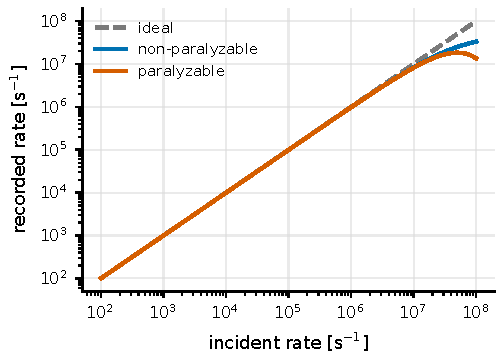
\includegraphics[width=0.72\linewidth]{figures/generated/chapter_06/ch06_deadtime_saturation.pdf}
\caption{入射计数率升高时，死时间使记录计数率偏离理想直线。非麻痹型趋向饱和值 \(1/\tau_d\)，麻痹型在极高通量下反而下降。图中取 \(\tau_d=20\,{\rm ns}\)，代表高速单光子通道的数量级；真实仪器需要用可调强度光源单独测量 \(\tau_d\) 与模型类型。}
\label{fig:e13-deadtime-saturation}
\end{figure}

死时间还提示了强度干涉常用的一招：把光\textbf{分束到两个独立探测器}做互相关（HBT 的做法，见第 \ref{chap:e10} 章）。因为死时间是\emph{每个探测器各自}的，两个探测器不会因为对方在死时间而漏掉零延迟附近的符合；这样既提高了可承受的总计数率，又顺带压掉了下一节要讲的同通道 afterpulsing \citep{1957RSPSA.242..300B,1996ApOpt..35.1956C,2020RScI...91a3108W}。

\section{Afterpulsing：探测器自造的短延迟假相关}
\label{sec:e13-afterpulse}

死时间让事件\emph{变少}，afterpulsing 却让事件\emph{无中生有}。在雪崩型器件（SPAD、SiPM）里，一次雪崩会有部分载流子被材料缺陷"抓住"（陷阱，trap），过一会儿又被释放，重新触发一次和天体光子毫无关系的二次脉冲——这就是\textbf{余脉冲}（afterpulse）。它危险的地方在于：这些假脉冲总是紧跟在真实脉冲后面几 ns 到几 \(\mu\)s，恰好落在我们最关心的\emph{短延迟}区间，会在自相关里伪造出一个假峰，被误读成"光子结伴到达"。

把它写成率的形式。设每个真实事件产生一个 afterpulse 的概率是 \(\epsilon_{\rm ap}\)，这些余脉冲相对主脉冲的延迟服从归一化分布 \(k_{\rm ap}(\tau)\)，那么额外的事件率是
\begin{equation}
  R_{\rm ap}(\tau)=\epsilon_{\rm ap}\,R_{\rm det}\,k_{\rm ap}(\tau),
  \qquad
  \int_0^\infty k_{\rm ap}(\tau)\,d\tau=1.
  \label{eq:e13-afterpulse}
\end{equation}
\begin{formulaexplain}
\(R_{\rm ap}\) 是余脉冲贡献；\(\epsilon_{\rm ap}\) 是每个真实事件产生余脉冲的概率；\(R_{\rm det}\) 是真实探测率；\(k_{\rm ap}\) 是归一化延迟核。它描述探测器\emph{自己制造}的短延迟假相关。
\end{formulaexplain}
逐项落实。\(\epsilon_{\rm ap}\) 无量纲，随器件与门控方式在 \(10^{-4}\)--\(10^{-2}\) 之间；\(R_{\rm det}\) 是式 \eqref{eq:e13-detected-rate} 给出的探测率（\({\rm s}^{-1}\)）；\(k_{\rm ap}(\tau)\) 单位是 \({\rm s}^{-1}\)（因为对 \(\tau\) 积分归一），它的特征时间从 ns 到 \(\mu\)s 不等。式子结构是"真实事件率 × 单次余脉冲概率 × 延迟分布"，非常好记。

怎么和真信号区分开？两个办法。第一，\emph{对同一探测器}做自相关，你会看到 afterpulse 峰赫然出现在短延迟处；第二，\emph{对两个独立探测器}做互相关，因为 A、B 两个探测器的陷阱释放彼此独立、不同步，余脉冲不会在互相关里制造符合，于是被大幅压制。这又一次说明了 HBT 分束互相关的双重好处：既解决死时间，又躲开 afterpulsing——同一份光，分给两只"互不知情"的探测器，谁也没法用自己的毛病去污染彼此的符合计数 \citep{1957RSPSA.242..300B,1996ApOpt..35.1956C,2020RScI...91a3108W}。

\section{时钟与同步：把两台望远镜放到同一根时间轴上}
\label{sec:e13-clock}

到这里，一台望远镜内部的事件表已经建立好了。可强度干涉、甚长基线计时至少需要\emph{两台}望远镜，它们各自的事件表只有放到\emph{共同的时间轴}上才能相关。这就要求两站的时钟对齐得足够准。多准才够？这里有一条贯穿全书的换算，把"时间精度"翻译成"光走的距离"：
\begin{equation}
  \Delta\ell = c\,\Delta t .
  \label{eq:e13-lightpath}
\end{equation}
\begin{formulaexplain}
\(\Delta t\) 是两站时钟对齐的残差，\(c\) 是光速，\(\Delta\ell\) 是这段时间里光走过的距离。它把"同步到多少皮秒"直接换算成"等价于多少厘米光程"。
\end{formulaexplain}
这条式子其实就是第 \ref{chap:e01} 章用到的"时间-光程"对应，只是这次用在时钟上。代数字（CGS，\(c=3\times10^{10}\,{\rm cm\,s^{-1}}\)）：\(\Delta t=1\,{\rm ns}=10^{-9}\,{\rm s}\) 对应 \(\Delta\ell=30\,{\rm cm}\)；\(\Delta t=100\,{\rm ps}\) 对应 \(3\,{\rm cm}\)；\(\Delta t=1\,{\rm ps}\) 对应 \(0.3\,{\rm mm}\)。所以"把两站同步到皮秒-纳秒"，物理上就等价于"把两条光路的长度对齐到毫米-厘米"——一个非常直观的尺度。反过来，只要你把时钟对齐到几十皮秒，几厘米以内的光程差就被时钟吸收掉了。

实现这种同步有两条主流路线。一是\textbf{GPS 授时}：卫星广播的秒脉冲（PPS，pulse per second）给每站一个共同的绝对时刻，配上本地铷钟保持短期稳定；AquEYE/Iqueye 用铷钟加 GPS PPS，把\emph{相对}时间精度做到约 100 ps rms、\emph{绝对} UTC 精度控制在 \(0.5\,{\rm ns}\) 以内 \citep{2009A&A...508..531N,2015SPIE.9504E..0CZ}。二是 \textbf{White Rabbit}：一种基于以太网加精密相位测量的光纤同步协议，把一个主时钟通过光纤分发到各站并实时补偿光纤长度，5 km 光纤链路测试得到约 39 ps 的同步贡献——按式 \eqref{eq:e13-lightpath} 换算，只等价于约 1.2 cm 的光程残差 \citep{2013NIMPA.725..187J,2020RScI...91a3108W}。

有了共同时钟，还要扣掉一个更大的、\emph{随时间变化}的项——几何延迟。同一束星光到达两站的时刻本就不同，因为两站到源的光程不等。对一对站点 \(a,b\)：
\begin{equation}
  \Delta t_{\rm geo}(t)
  =
  \frac{\mathbf{B}_{ab}(t)\cdot\hat{\mathbf{s}}}{c},
  \qquad
  \mathbf{B}_{ab}=\mathbf{r}_b-\mathbf{r}_a .
  \label{eq:e13-geometric-delay}
\end{equation}
\begin{formulaexplain}
\(\Delta t_{\rm geo}\) 是两站几何延迟；\(\mathbf B_{ab}\) 是基线向量（由两站位置之差给出），\(\hat{\mathbf s}\) 是源方向单位矢量，\(c\) 是光速。它把空间基线\emph{投影}成两路事件表需要相互平移的时间量。
\end{formulaexplain}
\(\mathbf B_{ab}\) 单位是 m，\(\hat{\mathbf s}\) 无量纲，点积 \(\mathbf B_{ab}\cdot\hat{\mathbf s}\) 是基线在源方向上的投影长度，除以 \(c\) 就是时间。代数字：100 m 基线最高约 \(\Delta t_{\rm geo}=100/(3\times10^8)\approx333\,{\rm ns}\)（此最大值出现在源方向与基线平行、即近地平时；反之源在天顶、基线近水平时投影 \(\mathbf B_{ab}\cdot\hat{\mathbf s}\approx0\)，几何延迟接近零），1 km 基线约 \(3.3\,\mu{\rm s}\)——远大于皮秒级的探测器抖动，可见几何延迟是相关里\emph{最大}的时间项，必须先扣掉才能对齐零延迟。更麻烦的是它\emph{随时间漂移}：地球自转让投影基线不断改变，一个 100 m 基线在天顶（中天）附近漂移最快，延迟变化速度约 \(\Omega_\oplus B/c\sim2.4\times10^{-11}\,{\rm s\,s^{-1}}\)，其中 \(\Omega_\oplus\approx7.3\times10^{-5}\,{\rm rad\,s^{-1}}\) 是地球自转角速度；这意味着每 1 秒就漂约 \(24\,{\rm ps}\)（17 分钟累计约 \(25\,{\rm ns}\)）——对皮秒级峰形，这不能用一个常数延迟一劳永逸地吸收。VERITAS-SII 对每个相关帧移动时间 lag 校正几何光程，MAGIC-SII 在 Pearson 相关后施加可变时间延迟校正 \citep{2020NatAs...4.1164A,2024MNRAS.529.4387A}。

若还要把光子折叠到脉冲星相位、或与其他波段的到达时刻比较，站点时间还得进一步转换到\emph{太阳系质心}（Solar System barycenter, SSB），加上一串标准改正项——本地时钟到坐标时的转换、Roemer 光行时（地球绕日轨道给出最高约 \(\pm500\,{\rm s}\)）、Einstein 引力/运动钟速改正、Shapiro 引力延迟、大气延迟。这些改正 Tempo2 已做到 ns 级，barycorrpy 和 Astropy 提供 Python 工作流接口 \citep{2006MNRAS.369..655H,2006MNRAS.372.1549E,2018RNAAS...2....4K,2013A&A...558A..33A,2018AJ....156..123A}。这些属于绝对计时的进阶内容，本章只需记住：同夜强度相关看\emph{相对}延迟，脉冲相位和多信使比较才需要\emph{绝对}的质心时间。

\begin{figure}[tbp]
\centering
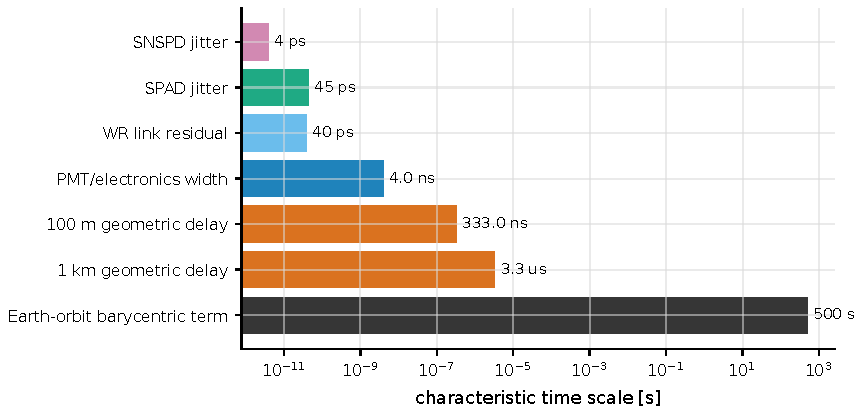
\includegraphics[width=0.84\linewidth]{figures/generated/chapter_06/ch06_time_budget.pdf}
\caption{同一份事件表会同时遇到皮秒、纳秒、微秒和百秒量级的时间项。探测器抖动与 White Rabbit 残差决定相关峰能否保持窄形；电子与镜面响应决定 ns 级强度干涉峰宽；几何延迟由基线长度与源方向决定，并随地球自转漂移；太阳系质心改正虽不是同夜峰宽项，却是脉冲相位、跨夜合并与多信使比较的绝对时间基础。}
\label{fig:e13-time-budget}
\end{figure}

把这些延迟一并写进标定事件表，原始计数器时间就变成了可跨站比较的物理时间：
\begin{equation}
  t^{\rm cal}_q =
  t^{\rm raw}_q
  +\Delta_{\rm clk}(t_q)
  +\Delta_{\rm elec}(a_q,d_q)
  +\Delta_{\rm det}(\lambda_q,d_q)
  -\frac{\mathbf{r}_{a_q}(t_q)\cdot\hat{\mathbf{s}}}{c}.
  \label{eq:e13-calibrated-time}
\end{equation}
\begin{formulaexplain}
\(t_q^{\rm cal}\) 是校正后事件时间；\(\Delta_{\rm clk},\Delta_{\rm elec},\Delta_{\rm det}\) 分别改正时钟、电子链路、探测器延迟；最后一项扣除几何光行时。它把不同站点放到共同时间轴。
\end{formulaexplain}
\(\Delta_{\rm clk}\) 是本站时钟相对统一时间尺度的偏移（几十皮秒到 ns），\(\Delta_{\rm elec}\) 是电缆、放大器、鉴别器、ADC/TDC 通道的固定或缓慢漂移延迟（常用脉冲源和环回链路标定），\(\Delta_{\rm det}\) 是探测器内部延迟（可能依赖波长、偏压、温度、脉冲高度），最后一项就是式 \eqref{eq:e13-geometric-delay} 的几何延迟。这条式子把前面几节的所有延迟项收进一个统一的时间标定框架里。

\section{事件表的字段：每一列为什么都要保留}
\label{sec:e13-schema}

现在可以回答本章开头那个最实用的问题了：事件表到底该存哪些字段？答案是分\emph{三层}存，而且原始层永远不可被后处理覆盖。

\textbf{原始层}保存式 \eqref{eq:e13-raw-event} 那些"最贴近电子学"的量：计数器 tick \(n_q\)、望远镜/站点编号 \(a_q\)、探测器编号 \(d_q\)、波长通道 \(c_q\)、偏振通道 \(p_q\)、质量标记 \(f_q\)、权重 \(w_q\)。为什么每一列都不能省？因为它们各自对应一种\emph{事后还想重做}的选择：留着 \(n_q\) 才能重新分箱、重新做延迟校正；留着 \(a_q,d_q\) 才能做\emph{互}相关而非自相关（从而躲开死时间与 afterpulsing）；留着 \(c_q\) 才能事后按波长重新选频；留着 \(p_q\) 才能重建偏振（偏振重建留待后续章节，见第 \ref{chap:e22} 章）；留着 \(f_q\) 才能追溯异常峰的来历；留着 \(w_q\) 才能做加权分析。一旦这一层被压成光变曲线，上面这些"重做"就全部失效。

\textbf{标定层}把原始 tick 通过式 \eqref{eq:e13-calibrated-time} 变成统一时间轴上的物理时间，并补上望远镜姿态、波长、偏振、权重等物理量。它是"每个分析版本"的产物，可以随标定改进而更新，但每次都要记录用了哪套改正。\textbf{相关产品层}才记录基线、延迟网格、bin 宽、相关幅度、剔除条件与协方差——也就是 \(g^{(2)}(\tau)\)、\(|V|^2\) 或脉冲到达时刻这些"成品"。

数据量有多大？由事件率和每事件字节数决定：
\begin{equation}
  \dot{M}
  \simeq
  N_{\rm tel}\,N_{\rm ch}\,R_{\rm evt}\,N_{\rm byte}.
  \label{eq:e13-data-rate}
\end{equation}
\begin{formulaexplain}
\(\dot M\) 是数据率；\(N_{\rm tel}\) 是望远镜数，\(N_{\rm ch}\) 是每台通道数，\(R_{\rm evt}\) 是单通道事件率，\(N_{\rm byte}\) 是每事件字节数。它估算事件表或波形流的存储压力。
\end{formulaexplain}
\(\dot M\) 单位 \({\rm byte\,s^{-1}}\)。代数字：\(N_{\rm tel}=4\)、\(N_{\rm ch}=8\)、\(R_{\rm evt}=10^6\,{\rm s^{-1}}\)、\(N_{\rm byte}=16\)，则 \(\dot M\simeq4\times8\times10^6\times16=5.12\times10^8\,{\rm byte\,s^{-1}}\approx512\,{\rm MB\,s^{-1}}\)。连续波形采样更凶：VERITAS-SII 以 250 MS/s 连续数字化每台望远镜的 PMT 信号，单望远镜约 250 MB/s，整次实验数据量达几十 TB \citep{2020NatAs...4.1164A}。存储格式上，FITS 的 BINTABLE 扩展适合长期归档和天文软件互操作，HDF5/Parquet 适合高吞吐列式筛选；Astropy 提供 FITS、坐标与时间处理接口，方便把事件表、时间尺度转换和质心改正放进同一条 Python 分析链 \citep{2010A&A...524A..42P,2013A&A...558A..33A,2018AJ....156..123A}。

分层的意义，一句话：让日后的读者能\emph{从同一份原始数据}重新生成光变曲线、\(g^{(2)}(\tau)\)、空间可见度或脉冲到达时刻，而不必去猜早期脚本悄悄做了哪些选择。可复现，是事件表设计的最高准则。

\section{谱分辨与相干时间的权衡}
\label{sec:e13-spectral}

最后一个字段值得单独讲：波长通道 \(c_q\)。给每个光子标上波长，不只是为了做光谱，更是因为\emph{波长通道的宽窄直接决定相干时间}，而相干时间又决定相关峰的固有宽度。回忆第 \ref{chap:e02} 章、第 \ref{chap:e08} 章：通道越窄，电场的相位记忆越长。定量地，若通道近似矩形、中心波长 \(\lambda\)、宽度 \(\Delta\lambda\)：
\begin{equation}
  \tau_c
  \simeq
  \frac{1}{\Delta\nu}
  \simeq
  \frac{\lambda^2}{c\,\Delta\lambda}
  =
  \frac{R\,\lambda}{c},
  \qquad
  R=\frac{\lambda}{\Delta\lambda}.
  \label{eq:e13-coherence-time}
\end{equation}
\begin{formulaexplain}
\(\tau_c\) 是相干时间；\(\Delta\nu\) 是频率带宽；\(\lambda,\Delta\lambda\) 是中心波长与波长带宽；\(R=\lambda/\Delta\lambda\) 是光谱分辨率。窄通道让相位记忆变长，但单通道光子率变低。
\end{formulaexplain}
中间两步不要跳。第一步 \(\tau_c\simeq1/\Delta\nu\) 是第 \ref{chap:e02} 章的带宽-相干时间关系。第二步把 \(\Delta\nu\) 换成波长量：由 \(\nu=c/\lambda\) 求微分，\(|d\nu|=(c/\lambda^2)\,|d\lambda|\)，所以 \(\Delta\nu\simeq c\Delta\lambda/\lambda^2\)，代入得 \(\tau_c\simeq\lambda^2/(c\Delta\lambda)\)。第三步认出 \(R=\lambda/\Delta\lambda\)，于是 \(\lambda^2/(c\Delta\lambda)=(\lambda/\Delta\lambda)(\lambda/c)=R\lambda/c\)。三步都是恒等变形，没有额外近似。

代数字（\(\lambda=500\,{\rm nm}\)）：\(R=100\Rightarrow\tau_c\simeq100\times500\times10^{-9}/(3\times10^8)\approx0.17\,{\rm ps}\)；\(R=10^4\Rightarrow\tau_c\simeq17\,{\rm ps}\)；\(R=10^5\Rightarrow\tau_c\simeq170\,{\rm ps}\)。注意：即便 \(R=10^5\)，\(\tau_c\) 仍短于多数 PMT/电子链的 ns 响应，所以照第 \ref{sec:e13-jitter} 节的结论，实际相关峰宽\emph{仍由仪器决定}；提高 \(R\) 拉长的是相位记忆（进而影响峰\emph{高}里电子带宽与光学带宽之比），而不是让峰变窄。

于是就有了本章最后一个权衡。提高 \(R\)（用更窄的滤光片）会拉长 \(\tau_c\)、让相干性更"纯"，但同时把单通道光子率压低约 \(1/R\)（带宽窄了，进来的光子少了）。想两头都要，就得\emph{同时读出更多波长通道}把总通量补回来：多通道 TCSPC 可以把不同波长当独立输入、输出单一时间排序的数据流；而 MAGIC、VERITAS 的 SII 系统则反其道，选少数宽滤光片通道来换取更高光子率——VERITAS 用中心 416 nm、有效宽度 13 nm 的滤光片，MAGIC 用 425 nm、26 nm 的干涉滤光片 \citep{2020NatAs...4.1164A,2024MNRAS.529.4387A,1974iiia.book.....H}。选宽还是选窄，取决于科学目标：测恒星直径，宽通道提信噪比就好；而要看发射线、吸收线或快速旋转星的速度结构，分波长相关能直接给出"空间信息随速度怎么变"，这时窄通道的代价就值得付。

\begin{figure}[tbp]
\centering
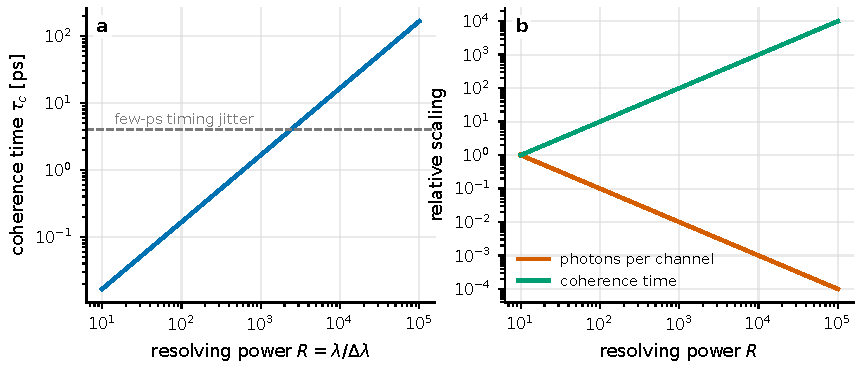
\includegraphics[width=0.92\linewidth]{figures/generated/chapter_06/ch06_spectral_resolution_coherence.pdf}
\caption{光谱分辨率与相干时间的数量级关系。左图固定 \(\lambda=500\,{\rm nm}\)，显示 \(\tau_c\simeq R\lambda/c\) 随分辨率线性增长；右图显示单通道光子率约随 \(1/R\) 降低，而相干时间随 \(R\) 增加。理想强度干涉的信噪比对光学带宽的依赖会部分抵消，但真实仪器还受滤光片形状、探测器响应、背景与电子带宽限制。}
\label{fig:e13-spectral-resolution-coherence}
\end{figure}

\section{本章要点}
\label{sec:e13-summary}

\begin{itemize}
  \item \textbf{光子变事件要过几道关卡。}量子效率 \(\eta\) 决定"多少光子变事件"（式 \eqref{eq:e13-detected-rate}）；PMT 大面积高增益、SPAD/SiPM 单光子皮秒计时但受面积、死时间、afterpulsing 限制，各有取舍。
  \item \textbf{抖动把相关峰卷宽、峰高稀释。}观测峰是真实峰与仪器响应的卷积（式 \eqref{eq:e13-response-convolution}）；独立高斯展宽按方差相加 \(\sigma_{\rm obs}^2=\sum\sigma_i^2\)（式 \eqref{eq:e13-jitter-budget}）。可见光 \(\tau_c\sim\)ps 远小于 ns 级响应，故峰宽几乎全由仪器决定，峰高被 \(\sim\sigma_{\rm sky}/\sigma_{\rm obs}\) 稀释——呼应第 \ref{chap:e08} 章。
  \item \textbf{死时间让记录率饱和，且分两型。}非麻痹型 \(r_{\rm rec}=r/(1+r\tau_d)\)（式 \eqref{eq:e13-nonparalyzable}）高通量饱和到 \(1/\tau_d\)；麻痹型 \(r_{\rm rec}=re^{-r\tau_d}\)（式 \eqref{eq:e13-paralyzable}）在 \(r\tau_d=1\) 达峰后回落。弱光下两者一致，强光下天差地别，必须实测判型。
  \item \textbf{afterpulsing 伪造短延迟假峰。}余脉冲率 \(R_{\rm ap}=\epsilon_{\rm ap}R_{\rm det}k_{\rm ap}(\tau)\)（式 \eqref{eq:e13-afterpulse}）落在关键的短延迟区。分束到两个独立探测器做互相关，能同时化解死时间与 afterpulsing。
  \item \textbf{时钟同步等价于对齐光程。}\(\Delta\ell=c\Delta t\)（式 \eqref{eq:e13-lightpath}）：100 ps \(\leftrightarrow\) 3 cm、1 ns \(\leftrightarrow\) 30 cm。GPS/White Rabbit 把两站对齐到几十皮秒；几何延迟 \(\Delta t_{\rm geo}=\mathbf B\cdot\hat{\mathbf s}/c\)（式 \eqref{eq:e13-geometric-delay}）最大（百米基线 \(\sim\)333 ns）且随地球自转漂移，须逐帧扣除。
  \item \textbf{事件表分三层、保原始信息。}原始层不可覆盖，标定层可迭代，相关产品层出成品；每个字段都对应一种"事后还想重做"的选择。可复现是最高准则。
  \item \textbf{谱分辨与相干时间此消彼长。}\(\tau_c\simeq R\lambda/c\)（式 \eqref{eq:e13-coherence-time}）：\(R\) 越大相干时间越长，但单通道光子率约降 \(1/R\)。选宽选窄取决于是测直径还是看速度结构。
\end{itemize}

\noindent\textbf{想一想。}(1) 若某 SPAD 的死时间曲线在高通量下先升后降，它更可能是哪一型？据此如何反推 \(\tau_d\)？(2) 把两站时钟对齐到 50 ps，等价于对齐多长的光程？这相对 100 m 基线的几何延迟是大是小？(3) 若把 \(R\) 从 100 提到 \(10^4\)，相干时间涨了多少倍，单通道光子率大约降到原来的几分之一？要保住总通量该怎么办？

\chapter{相关器与事件表数据分析}
\label{chap:e14}

\begin{chapteropening}
上一章（第 \ref{chap:e13} 章）里，望远镜把每一个光子候选写成了一行记录：什么时候到、来自哪个站点、走哪个探测器通道、什么波长、什么偏振。一夜下来，这样的记录可能有几十亿行——它们静静地躺在磁盘上，本身既不是角直径，也不是 \(g^{(2)}\)，只是一堆时间戳。

本章要回答的，正是横在"一堆事件"和"一条可信曲线"之间的那道工序：怎样把这几十亿个时间戳，变成一条带误差棒、能复现、能拿去拟合物理模型的 \(|V|^2\) 或 \(g^{(2)}\)？我们会沿着一条主线走：先把事件表翻译成概率模型（写出似然），再定义相关估计量并做归一化，然后解决"算得完吗"（相关器的计算量标度），最后是全书数据分析里最容易被低估的一环——误差从哪来、为什么系统误差往往才是天花板。第 \ref{chap:e08} 章给过的延迟直方图、第 \ref{chap:e12} 章给过的 Fisher 语言，会在这里被真正用起来。
\end{chapteropening}

\section{从事件表到概率模型}
\label{sec:e14-model}

先约定记号。把一份标定后的事件表整体记作一个数据集
\begin{equation}
  \mathcal{D}
  =
  \left\{
  t_q,\ a_q,\ d_q,\ c_q,\ p_q,\ w_q,\ f_q
  \right\}_{q=1}^{N_{\rm evt}} ,
  \label{eq:e14-data}
\end{equation}
\begin{formulaexplain}
\(\mathcal D\) 是整张标定事件表；每个事件 \(q\) 带时间 \(t_q\)、站点 \(a_q\)、探测器 \(d_q\)、谱道 \(c_q\)、偏振 \(p_q\)、权重 \(w_q\) 和质量标记 \(f_q\)；\(N_{\rm evt}\) 是总事件数。它是后面一切估计量的原始"食材"。
\end{formulaexplain}
这里 \(t_q\) 是统一时间尺度上的到达时刻（单位 s，典型精度可达纳秒甚至几十皮秒），\(a_q,d_q,c_q,p_q\) 都是整数通道编号（无量纲），\(w_q\) 是权重（无量纲），\(f_q\) 是标记这条事件是否"干净"的质量位。这些字段怎么来、时钟怎么校、格式怎么定，是上一章（第 \ref{chap:e13} 章）的内容；这一章直接从"表已经在手上"开始。

分析的第一步不是画图，而是写下一个\textbf{选择函数}（selection function），它决定哪些事件参与后续计算：
\begin{equation}
  S_q = S(t_q,a_q,d_q,c_q,p_q,f_q),
  \qquad
  S_q\in\{0,1\}\ \text{或}\ [0,1] .
  \label{eq:e14-selection}
\end{equation}
\begin{formulaexplain}
\(S_q\) 是第 \(q\) 个事件的选择/权重；取 0 或 1 表示剔除或保留，取 \([0,1]\) 的连续值表示曝光、死时间、背景或效率带来的加权。它把"人为选点"变成一条能重跑的规则。
\end{formulaexplain}
为什么要如此正式？想象一个通道事件率是 \(10^{6}\,\mathrm{s^{-1}}\)，一小时观测就是 \(3.6\times10^{9}\) 个事件。谁也没法"看着图手动删几个坏点"——那既做不到，也不可复现。选择函数必须能由元数据（云量、PMT 电流、死时间标记、阈值）自动重新生成，这样光变、相关、拟合三层用的都是同一套口径。第 \ref{chap:e15} 章做误差预算时会反复强调：一切系统检验都要在同一套 \(S_q\) 下进行。

\paragraph{未分箱数据：非齐次泊松点过程}

事件在时间轴上是一个个离散的点，最自然的模型是\textbf{非齐次泊松点过程}（inhomogeneous Poisson point process）：某时刻、某通道的瞬时事件率是 \(\lambda(t,\bm{x}\mid\bm{\theta})\)，其中 \(\bm x\) 打包了通道、波长、偏振、天空位置等标签，\(\bm\theta\) 是我们最终想估计的物理参数。第 \ref{chap:e03} 章讲过：泊松过程里"很短一段时间内出现一个事件"的概率正比于率乘以时长，而且互不影响。我们就用这一点把似然一步步搭出来。

把整段观测切成许多极窄的小格 \(\Delta t\)，窄到每格里至多一个事件。第 \(i\) 格里"有一个事件"的概率约为 \(\lambda_i E_i\,\Delta t\)（\(E_i\) 是这一格的有效曝光），"没有事件"的概率约为 \(1-\lambda_i E_i\,\Delta t\approx e^{-\lambda_i E_i\Delta t}\)。整段观测的似然就是所有格子的连乘：占据的格子贡献 \(\lambda E\Delta t\)，空格子贡献 \(e^{-\lambda E\Delta t}\)。取对数：
\[
  \ln L
  =\sum_{q:\,S_q>0}\ln\!\big(\lambda(t_q,\bm x_q)\,E_q\,\Delta t\big)
   -\sum_{\text{所有格}}\lambda_i E_i\,\Delta t .
\]
让 \(\Delta t\to0\)：第一项里的 \(\ln\!\big(\lambda E_q\,\Delta t\big)=\ln\lambda+\ln E_q+\ln\Delta t\) 可以拆开，其中 \(\ln\Delta t\) 是分箱宽度、\(\ln E_q\) 是这一格的仪器/曝光项，二者都与待估参数 \(\bm\theta\) 无关，拟合时作为常数一起丢掉（注意曝光 \(E\) 本身并没有消失，它仍完整保留在第二项的积分里），故第一项只剩 \(\ln\lambda\)；第二个求和变成积分。于是
\begin{equation}
  \ln L(\bm\theta)
  =
  \sum_{q:\,S_q>0}\ln\lambda(t_q,\bm x_q\mid\bm\theta)
  -\int_{\mathcal T}\lambda(t,\bm x\mid\bm\theta)\,E(t,\bm x)\,dt\,d\bm x .
  \label{eq:e14-point-likelihood}
\end{equation}
\begin{formulaexplain}
\(\ln L\) 是点过程对数似然。第一项在每个真实事件处给模型率打分：事件落在高率区就加分。第二项是模型在有效曝光 \(E\) 上预言的总事件数：模型不能只在事件处冒尖，还得解释别处为什么没事件。
\end{formulaexplain}
逐个符号说清楚：\(\lambda\) 的单位是 \(\mathrm{s^{-1}}\)（或 \(\mathrm{s^{-1}\,channel^{-1}}\)），\(E(t,\bm x)\) 无量纲或带面积/效率因子，装的是坏天气、死时间、通道开关、滤光片透过率、观测窗口这些真实损耗。这条式子最重要的教学点是它的"平衡"：只让率在事件处高是骗不过第二项的，因为第二项会因预言太多事件而扣分。这正是天文学里的 Cash 统计量（Cash statistic），低计数时不能用对称的 \(\sqrt N\) 误差蒙混过去 \citep{1979ApJ...228..939C,1986ApJ...303..336G}。

\begin{figure}[tbp]
\centering
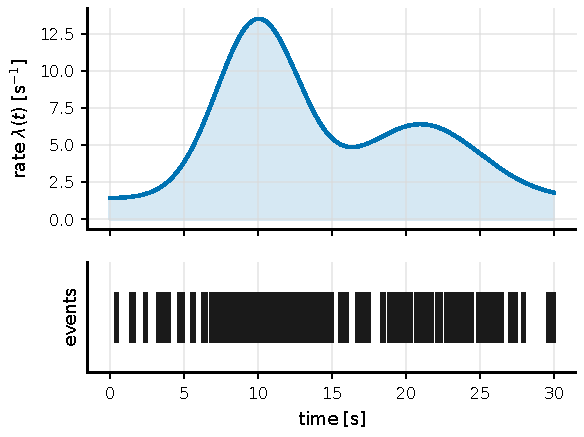
\includegraphics[width=0.72\linewidth]{figures/generated/chapter_07/ch07_poisson_likelihood.pdf}
\caption{非齐次泊松过程的画面。上图是随时间起伏的瞬时率 \(\lambda(t)\)，下图是由这个率随机"落下"的一串事件。似然式 \eqref{eq:e14-point-likelihood} 同时用到"事件落在高率处"和"整段积分率"两条信息；若只把事件重新分箱成一条光变曲线，就会丢掉一部分时间信息，快变或曝光不均时尤其明显。}
\label{fig:e14-poisson}
\end{figure}

\paragraph{分箱数据：退化成逐格泊松}

如果我们先把事件分进时间格、谱道或延迟格，点过程似然就退化成人人熟悉的\textbf{分箱泊松似然}。第 \(i\) 格观测到 \(d_i\) 个事件、模型预言 \(m_i(\bm\theta)\) 个，泊松概率是 \(P(d_i)=e^{-m_i}m_i^{d_i}/d_i!\)（见第 \ref{chap:e03} 章）。各格独立，取对数再求和：
\begin{equation}
  \ln L
  =\sum_i\Big[\,d_i\ln m_i(\bm\theta)-m_i(\bm\theta)-\ln(d_i!)\,\Big] .
  \label{eq:e14-binned-poisson}
\end{equation}
\begin{formulaexplain}
\(d_i\) 是第 \(i\) 格的观测计数，\(m_i\) 是模型计数，二者都无量纲。这是光变曲线、谱道、延迟直方图都能用的似然；它天生保留低计数时的不对称统计，不假装误差是高斯的。
\end{formulaexplain}
当某格计数 \(d_i\gtrsim20\) 且模型不贴边界时，泊松可近似成高斯，误差棒近似 \(\sqrt{d_i}\)；但当格子计数只有几个（延迟直方图的信号窗口常如此），就必须留在式 \eqref{eq:e14-binned-poisson}。还有一个坑要提前说：当模型里新增一个"强度必须非负"的分量（例如"有没有相关峰"），零强度落在参数边界上，似然比检验不再服从名义 \(\chi^2\) 分布，显著性得靠模拟或后验预测检验来标定 \citep{2002ApJ...571..545P}。对慢变背景和爆发筛选，Bayesian Blocks 会把时间轴自适应地切成若干"常率段"，数据空隙通过有效曝光（live time）进入而不被误认作"无事件" \citep{2013ApJ...764..167S}；但最终物理参数仍应回到明确的似然。

\section{两路事件如何长出相关峰}
\label{sec:e14-corr}

强度干涉的核心动作，是比较两个站点 \(a,b\) 的事件到达时间。第 \ref{chap:e08} 章已经从 \(g^{(2)}\) 得到过延迟直方图的思想；这里把它落成能对真实事件表运行的估计量。

第一步是算\textbf{校正后的时间差}。原始时间差里混着几何延迟和仪器延迟，必须先扣掉：
\begin{equation}
  \tau_{ij}^{ab}
  =
  t_{j,b}^{\rm cal}-t_{i,a}^{\rm cal}
  -\Delta t_{\rm geo}^{ab}(t_i,\hat{\bm s})
  -\Delta t_{\rm inst}^{ab}(t_i) .
  \label{eq:e14-delay}
\end{equation}
\begin{formulaexplain}
\(\tau_{ij}^{ab}\) 是站点 \(a,b\) 两事件校正后的延迟；\(t^{\rm cal}\) 是标定时间，\(\Delta t_{\rm geo}\) 扣几何（波前先到近端望远镜），\(\Delta t_{\rm inst}\) 扣两路残余仪器延迟。它决定这一对事件落进哪个延迟格。
\end{formulaexplain}
几何延迟为什么不能忽略？对 100 m 基线，波前抵达两台望远镜的最大时差约 \(100/c\approx333\,\mathrm{ns}\)；1 km 基线则是 \(3.3\,\mu\mathrm{s}\)。若延迟格宽 \(\Delta\tau=4\,\mathrm{ns}\)，几何延迟只要算错一个格，相关峰就被推离零延迟、直接消失。更进一步，地球在自转，投影基线 \(\hat{\bm s}\) 方向随时间变，几十皮秒精度时几何延迟得在很短的时间块里不断更新 \citep{2006MNRAS.369..655H,2006MNRAS.372.1549E,2018RNAAS...2....4K,2020NatAs...4.1164A}。

第二步是数对：把所有延迟落在第 \(k\) 个格 \(\tau_k\pm\Delta\tau/2\) 内的事件对数出来：
\begin{equation}
  C_{ab,k}
  =\sum_{i\in a}\sum_{j\in b}
  S_iS_j\,
  \mathbf 1\!\left[\tau_k-\tfrac{\Delta\tau}{2}\le\tau_{ij}^{ab}<\tau_k+\tfrac{\Delta\tau}{2}\right] .
  \label{eq:e14-paircount}
\end{equation}
\begin{formulaexplain}
\(C_{ab,k}\) 是第 \(k\) 个延迟格里的事件对数；\(S_iS_j\) 给每对加权，指示函数 \(\mathbf 1[\cdot]\) 只挑延迟落在该格内的对。它就是延迟直方图的一根柱子，无量纲。
\end{formulaexplain}

\paragraph{归一化：相关峰是背景上的微弱超额}

一根柱子有多高，本身没意义——因为哪怕两路完全无关，纯随机也会撞出一堆"偶然符合"。设两路独立、率在活时间内近似稳定，偶然符合的期望可以这样估：\(a\) 路一共有 \(R_aT_{\rm live}\) 个事件，每个事件在延迟格 \(\Delta\tau\) 内"撞上"一个 \(b\) 路事件的概率约 \(R_b\Delta\tau\)，两者相乘：
\begin{equation}
  B_{ab,k}\simeq R_aR_b\,\Delta\tau\,T_{\rm live} .
  \label{eq:e14-accidental}
\end{equation}
\begin{formulaexplain}
\(B_{ab,k}\) 是随机符合背景；\(R_a,R_b\)（单位 \(\mathrm{s^{-1}}\)）是两路平均率，\(\Delta\tau\) 是格宽，\(T_{\rm live}\) 是扣掉坏时间后的积分时间。它是"无天体相关时"每格该有的偶然对数。
\end{formulaexplain}
代真实数字感受一下量级：取 \(R_a=R_b=10^{7}\,\mathrm{s^{-1}}\)、\(\Delta\tau=1\,\mathrm{ns}\)、\(T_{\rm live}=3600\,\mathrm{s}\)，得 \(B\approx10^{7}\times10^{7}\times10^{-9}\times3600\approx3.6\times10^{8}\)。背景高达几亿对，而天体相关只是它上面 \(10^{-6}\)–\(10^{-4}\) 量级的一点点超额 \citep{1974iiia.book.....H,2020NatAs...4.1164A,2024MNRAS.529.4387A}。把这两个数放一起就懂了：信号 \(\approx3.6\times10^{8}\times10^{-4}\approx3.6\times10^{4}\) 对，而背景的泊松涨落 \(\approx\sqrt{B}\approx1.9\times10^{4}\)——一小时下来信噪比才 \(\sim2\)。强度干涉之所以要积几十小时，答案就写在这里。

把柱子除以背景，得到归一化的二阶相关估计量和它的超额：
\begin{equation}
  \widehat g^{(2)}_{ab}(\tau_k)=\frac{C_{ab,k}}{B_{ab,k}},
  \qquad
  \widehat C_{ab}(\tau_k)=\widehat g^{(2)}_{ab}(\tau_k)-1 .
  \label{eq:e14-g2}
\end{equation}
\begin{formulaexplain}
\(\widehat g^{(2)}\) 是归一化二阶相关，\(\widehat C_{ab}\) 是相对随机背景的超额（无量纲）。强度干涉信号，就藏在这个减 1 之后的微小超额里。
\end{formulaexplain}
实践中很少直接用式 \eqref{eq:e14-accidental} 的解析背景，而是用\textbf{时移背景}（time-shift）来估 \(B\)：把 \(b\) 路整体平移一个 \(\Delta T_{\rm shift}\)，平移量要远大于相关峰宽（这样真信号被移走），又要远小于增益和率的慢变时间（这样背景结构被保留）。用多个正负平移取平均，就同时得到背景均值和背景不确定度。此外还有 off-source（估夜天光、暗电流）、off-band（谱线科学）、错偏振（找串扰）等替身。VERITAS-SII 在 1 秒相关帧上剔除高频电子噪声和低 PMT 电流帧，再对几何延迟校正后的帧加权平均；MAGIC-SII 用信号像素和背景像素的直流读数一起修正夜天光 \citep{2020NatAs...4.1164A,2024MNRAS.529.4387A}。

\begin{figure}[tbp]
\centering
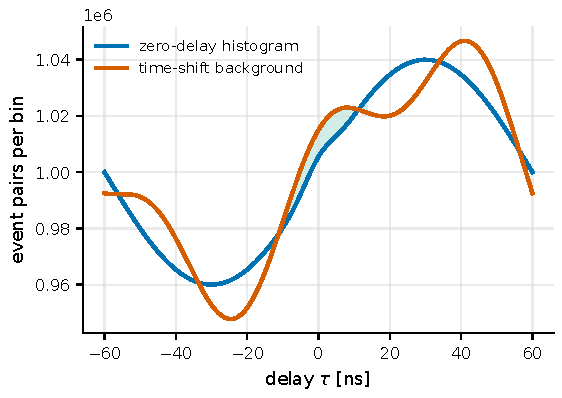
\includegraphics[width=0.72\linewidth]{figures/generated/chapter_07/ch07_time_shift_background.pdf}
\caption{时移背景估计的结构。蓝线是零延迟附近的事件对直方图，橙线是把一路整体平移到非物理延迟后得到的随机符合背景，绿色区域是中央峰相对时移背景的超额。这个方法能保留慢变率、坏时间和背景结构，但平移量必须远大于仪器响应宽度和天体相关宽度。}
\label{fig:e14-timeshift}
\end{figure}

\paragraph{连续波形的版本：Pearson 相关}

若硬件给的不是离散事件、而是连续采样的电压/电流波形（MAGIC-SII 就是），基本量改成\textbf{Pearson 相关系数}：
\begin{equation}
  \rho_{ab}(\tau_k)
  =\frac{\sum_n\big[x_a(t_n)-\bar x_a\big]\big[x_b(t_n+\tau_k)-\bar x_b\big]}
        {\sqrt{\sum_n\big[x_a(t_n)-\bar x_a\big]^2\;\sum_n\big[x_b(t_n)-\bar x_b\big]^2}} .
  \label{eq:e14-pearson}
\end{equation}
\begin{formulaexplain}
\(\rho_{ab}\) 衡量两路去均值波形的同步涨落；\(x_a,x_b\) 是采样电压/电流，\(\bar x\) 是各自平均。分母做归一，让 \(\rho\in[-1,1]\)；但它还混着恒星、夜天光、电子噪声，需再定标才成 \(|V|^2\)。
\end{formulaexplain}
Pearson 相关在硬件里实时算很方便（就是去均值、相乘、累加），但它测到的是三种涨落的混合，必须用直流电流、背景像素、零基线标定，才能转成物理的平方可见度 \(|V|^2\) \citep{2024MNRAS.529.4387A}。最后一个工程细节：格宽 \(\Delta\tau\) 要和相关峰宽、时间戳量化一起选——太宽会把峰高稀释掉，太窄则相邻格强相关、计算量白涨；VERITAS-SII 的相关 lag 间隔取 4 ns、峰宽也约 4 ns，而几十皮秒的 TDC 可以把格切得更细，前提是几何延迟、仪器响应、时钟残差都同等精度 \citep{2020NatAs...4.1164A,2020RScI...91a3108W,2009A&A...508..531N}。

\section{相关器如何在一夜之内算完}
\label{sec:e14-scaling}

现在面对一个纯工程问题：式 \eqref{eq:e14-paircount} 那个双重求和，真的能算完吗？

\textbf{最朴素的逐对法}。两路各有 \(N_a,N_b\) 个事件，全量比较就是 \(N_aN_b\) 次差分；若是同一路自相关，则是 \(N(N-1)/2\) 对。取 \(N_a=N_b=10^{9}\)，那是 \(10^{18}\) 次差分——即便每秒十亿次（\(10^{9}\,\mathrm{s^{-1}}\)，单核大致的现实速率），也要 \(10^{18}/10^{9}=10^{9}\,\mathrm s\approx30\) 年。逐对法只配用来做小样本教学检验。

\textbf{排序窗口法}。真相关峰只在很窄的延迟窗内，没必要比较相隔几秒的事件对。把两路都按时间排序，只在 \(|t_{j,b}-t_{i,a}|\le W\) 的滑动窗内找对，需检查的候选对数约为
\begin{equation}
  N_{\rm pair}^{\rm win}\simeq 2W\,R_b\,N_a .
  \label{eq:e14-window}
\end{equation}
\begin{formulaexplain}
\(N_{\rm pair}^{\rm win}\) 是窗口法要检查的候选对数；\(W\)（单位 s）是最大延迟窗半宽，\(R_b\) 是第二路率，\(N_a\) 是第一路事件数。有限窗把复杂度从 \(N^2\) 拉回近线性。
\end{formulaexplain}
代入 \(W=100\,\mathrm{ns}\)、\(R_b=10^{6}\,\mathrm{s^{-1}}\)、\(N_a=10^{9}\)：候选对约 \(2\times10^{-7}\times10^{6}\times10^{9}=2\times10^{8}\)，比全量双循环少了整整十个数量级，一台工作站几分钟就能扫完。而且排序窗口法保留每个事件的全部标签（波长、偏振），方便事后重新筛选。

\textbf{FFT 相关：XF 与 FX 两种排法}。若已经把事件或波形放进均匀时间格，可用快速傅里叶变换把时域互相关变成频域相乘：
\begin{equation}
  c_{ab}[k]
  =\mathcal F^{-1}\!\Big[\mathcal F\{x_a[n]\}^{*}\,\mathcal F\{x_b[n]\}\Big]_k .
  \label{eq:e14-fft}
\end{equation}
\begin{formulaexplain}
\(c_{ab}[k]\) 是离散互相关；\(\mathcal F,\mathcal F^{-1}\) 是离散傅里叶正/反变换，星号是复共轭。它把逐格相乘累加（\(O(N_{\rm bin}^2)\)）换成频域一次相乘（\(O(N_{\rm bin}\log N_{\rm bin})\)），\(N_{\rm bin}\) 是均匀时间格的格数（这里另起一个记号，别和后面误差预算里表示时移背景个数的 \(M\) 混淆）。
\end{formulaexplain}
这里就出现射电阵列里熟悉的两种相关器分工：\textbf{XF} 型先做互相关（correlate，得到延迟域的 \(c_{ab}[k]\)）再傅里叶变换成谱；\textbf{FX} 型反过来，先对每路各做一次 FFT（Fourier），再在每个频道上把各路两两相乘（cross-multiply）。为什么台站一多就偏爱 FX？因为 FFT 是"每路一次"的开销，随台站数 \(N_{\rm tel}\) 线性增长；而两两相乘那步无论哪种排法都是 \(O(N_{\rm tel}^{2})\)、躲不掉。台站少时（今天的强度干涉阵列往往只有 2–4 台，配对数 \(N(N-1)/2\) 很小），瓶颈根本不在配对数，而在\textbf{每对要吞的时间样本数}——这才是相关器真正的重活。

\begin{figure}[tbp]
\centering
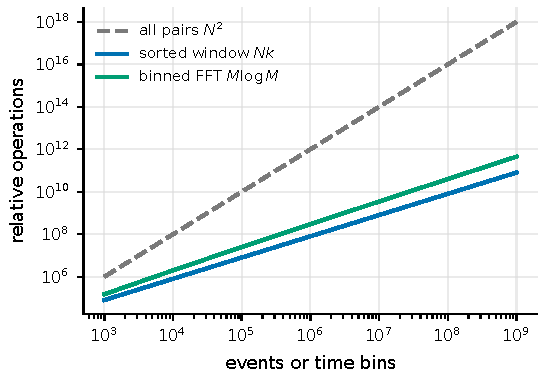
\includegraphics[width=0.72\linewidth]{figures/generated/chapter_07/ch07_correlator_scaling.pdf}
\caption{三类相关计算的操作数标度。全量逐对双循环随 \(N^2\) 疯长，只适合小样本或教学检验；排序窗口只比较有限延迟内的对，近似线性；均匀分箱后的 FFT 相关随 \(N_{\rm bin}\log N_{\rm bin}\) 增长，适合连续采样和实时监控。实际速度还受内存带宽、I/O、GPU/FPGA 数据排布和质量筛选左右。}
\label{fig:e14-scaling}
\end{figure}

\textbf{实时、无死时间的硬件相关}。VERITAS-SII 把连续 PMT 波形流到磁盘、再用 FPGA 离线相关；MAGIC-SII 则用 GPU 在观测当下实时算四通道所有配对相关 \citep{2020NatAs...4.1164A,2024MNRAS.529.4387A}。连续波形相关有一个单光子计数比不了的好处：它不靠"逐个光子触发—复位"，因此没有单光子探测器那种每次计数后的死时间盲区，能不间断地把整段涨落都算进相关里；这对信号只有 \(10^{-6}\)–\(10^{-4}\) 的强度干涉尤其重要，任何被丢掉的时间都是白扔的信噪比。多通道 TCSPC 则输出按时间排序的事件流，便于离线构造任意延迟和通道选择 \citep{2020RScI...91a3108W}。实时相关还能在观测中当场发现时钟跳变、电子串扰、云导致的通量突变——代价是通常只保存压缩后的相关产品。为长期归档，最好把原始事件/波形、标定事件、相关产品都留一份：FITS BINTABLE 适合事件归档，HDF5/Parquet 适合列式大数据，Astropy 帮着处理 FITS、时间和坐标元数据 \citep{2010A&A...524A..42P,2013A&A...558A..33A,2018AJ....156..123A}。

\section{误差为什么不是一串独立误差棒}
\label{sec:e14-cov}

到这里我们有了一条 \(\widehat g^{(2)}(\tau_k)\) 或一组 \(|V|^2\)。给每个点配一根 \(\sqrt N\) 误差棒、当作彼此独立，是初学者最常犯的错。先看理想情形下误差该有多大，再看真实数据为什么偏离它。

设信号窗计数 \(C_{ab,k}\) 是独立泊松量，背景由 \(M\) 个等权时移估计、\(\widehat B_{ab,k}=\frac1M\sum_{m=1}^{M}B_m\)，每个 \(B_m\) 是均值为 \(B\) 的独立泊松量。中央超额 \(X=C-\widehat B\) 的方差怎么算？泊松量方差等于均值，故 \(\operatorname{Var}(C)\approx C\)；背景平均后 \(\operatorname{Var}(\widehat B)=\frac1{M^2}\sum_m\operatorname{Var}(B_m)=\frac1{M^2}\,(M\,B)=B/M\)。两者独立、方差相加：
\begin{equation}
  \operatorname{Var}\!\big[\,C_{ab,k}-\widehat B_{ab,k}\,\big]
  \simeq C_{ab,k}+\frac{1}{M}\,B_{ab,k} .
  \label{eq:e14-excess-var}
\end{equation}
\begin{formulaexplain}
第一项 \(C_{ab,k}\) 是信号窗自身的泊松噪声，第二项 \(B_{ab,k}/M\) 是 \(M\) 个时移背景平均后的残余不确定度。\(M\) 越大，背景估得越稳。这是"事件独立、率稳定"理想下的误差预算。
\end{formulaexplain}
但式 \eqref{eq:e14-excess-var} 只在事件独立、时移背景互不重叠、率稳定时成立。真实数据里到处是"共享"：相邻延迟格共享同一批事件；多条基线共享同一台望远镜；多个波长通道共享同一片天气和同一路增益；多个模型点共享同一次零基线归一化。任何被共享的东西，都会让不同数据点的误差\textbf{相关}起来——误差矩阵不再是对角的。

于是要把全部相关产品当成一个向量、配一个协方差矩阵：
\begin{equation}
  \bm d=\big(\widehat{|V|^2}_1,\ \widehat{|V|^2}_2,\ \ldots,\ \widehat{|V|^2}_{N_d}\big),
  \qquad
  \Sigma_{ij}=\big\langle(d_i-\mu_i)(d_j-\mu_j)\big\rangle .
  \label{eq:e14-cov}
\end{equation}
\begin{formulaexplain}
\(\bm d\) 是相关产品数据向量，\(d_i\) 是第 \(i\) 个 \(|V|^2\) 点，\(\mu_i\) 是其均值；\(\Sigma_{ij}\) 是协方差矩阵，对角是各点方差，非对角记录"共享望远镜/背景/定标"造成的相关误差。
\end{formulaexplain}
\(\Sigma\) 从哪来？四条路子：解析误差传播（像式 \eqref{eq:e14-excess-var}）、时间块 bootstrap、jackknife（逐一剔除一台望远镜或一夜）、以及端到端注入仿真。时间块 bootstrap 是最实用的：把整夜数据切成许多时间块，块长要长于相关峰宽、电子噪声相关时间和指向/天气短时波动（夜级数据常取 10 s 到几分钟），随机有放回地重采样这些块、重算 \(|V|^2\)，块间的散布就直接给出协方差——顺带还检验了误差是否随积分时间以 \(T^{-1/2}\) 收敛。MAGIC-SII 就把电子带宽、光学带宽、直流读出增益、背景扣除、残余电子噪声都列成系统项，并通过朝极端方向摆动 \(|V|^2\) 数据点来估角直径的系统误差 \citep{2024MNRAS.529.4387A}。

\begin{figure}[tbp]
\centering
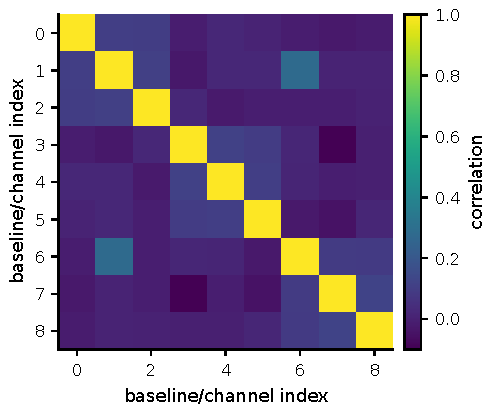
\includegraphics[width=0.66\linewidth]{figures/generated/chapter_07/ch07_covariance_matrix.pdf}
\caption{多基线/多通道结果的协方差矩阵示意。对角是单点方差，靠近对角的方块来自同一时间段或同一望远镜共享的噪声，远离对角线的结构可能来自共同背景估计、零基线归一化或电子串扰。若拟合只用对角误差，就会把"有效独立信息量"高估，误差棒假性变小。}
\label{fig:e14-cov}
\end{figure}

最后一句忠告：所有空检验（null test）都要用与主分析\textbf{同一套}选择函数和权重。常用空检验包括——把一路平移到非物理延迟、交换正负几何延迟、用两个本不该相关的偏振或波长通道、拿目标外天空当背景、把望远镜对分成不同时间块、逐一剔除某台望远镜或某夜、在真实事件表里注入已知相关峰看能否无偏恢复。若主信号只在某个阈值下冒头，一挪阈值、错延迟或做 jackknife 就消失，那它更可能是管线选择或仪器状态的产物，而不是天体相关。

\section{白噪声会沉降，系统误差是天花板}
\label{sec:e14-floor}

第 \ref{chap:e12} 章用 Fisher 信息回答过"数据里到底有多少信息"。这里把它接到时间上，讲清一个观测计划里最要命的分水岭：白噪声和系统误差，命运完全不同。

\textbf{白噪声（统计噪声）会沉降。}它来自光子的泊松涨落和电子的随机噪声，是一次次独立抽样。第 \ref{chap:e03} 章的结论：独立抽样越多，均值越稳，误差随有效光子数 \(N_{\rm eff}\) 以 \(N_{\rm eff}^{-1/2}\)、也就是随积分时间以 \(T^{-1/2}\) 下降。用 Fisher 语言说，独立数据点的信息是\textbf{相加}的，总信息随 \(N_{\rm eff}\) 线性增长，而 Cramér–Rao 下界给出的参数误差随信息平方根反比缩小——只要你肯积分，它就一直往下掉。

\textbf{系统误差（系统性偏差）不会沉降。}它来自定标不准、背景扣不干净、增益漂移、零基线不为零、电子带宽或光学带宽标定偏差这些\textbf{一致性偏移}。它们不是每次独立抽样，而是把每个数据点朝同一方向推同样一点点。再积分十倍时间，白噪声掉到 \(1/\sqrt{10}\)，可这个偏移纹丝不动——它成了一条水平的\textbf{地板}，误差再也下不去。

为什么这条地板对我们尤其致命？因为强度干涉的信号本就只有 \(10^{-6}\)–\(10^{-4}\) 那么微弱（回看式 \eqref{eq:e14-accidental} 下方那个 \(3.6\times10^4\) 对超额压在 \(3.6\times10^8\) 背景上的例子）。当你要测的超额只有百万分之一，那么背景定标只要有百万分之几的一致性偏差，就足以和信号同量级甚至淹没它。换句话说：微弱信号把系统误差的容忍度也压到了同样苛刻的 \(10^{-6}\) 级别，这正是本领域"系统项才是天花板"的根源。

把这句话数学化，就是把式 \eqref{eq:e14-cov} 的协方差喂进 Fisher 矩阵（推导见第 \ref{chap:e12} 章）：
\begin{equation}
  F_{\alpha\beta}
  =\frac{\partial\bm m^{T}}{\partial\theta_\alpha}\,\Sigma^{-1}\,\frac{\partial\bm m}{\partial\theta_\beta},
  \qquad
  \operatorname{Cov}(\theta_\alpha,\theta_\beta)\gtrsim(F^{-1})_{\alpha\beta} .
  \label{eq:e14-fisher}
\end{equation}
\begin{formulaexplain}
\(F_{\alpha\beta}\) 是 Fisher 信息矩阵：\(\partial\bm m/\partial\theta\) 是模型对参数的敏感度，\(\Sigma^{-1}\) 按协方差加权。其逆 \(F^{-1}\) 近似给出参数协方差下界。它是观测规划和高信噪比误差估计的主力工具。
\end{formulaexplain}
从这条式子能一眼读出两种标度。其一，\textbf{随光子数标度}：若 \(\Sigma\) 由独立光子统计主导，则 \(\Sigma^{-1}\propto N_{\rm eff}\)，\(F\propto N_{\rm eff}\)，参数误差 \(\propto N_{\rm eff}^{-1/2}\)——这就是白噪声的沉降。其二，\textbf{随基线标度}：Fisher 信息对相互独立的 \(uv\) 点是相加的，\(F=\sum_{\text{基线}}\)（各基线一项），所以多加一条基线就多一份信息。但一条基线值不值，取决于它落在模型 \(|V|^2\) 对参数最敏感、也就是 \(\partial\bm m/\partial\theta\) 最大的地方：对测角直径，最有价值的基线落在可见度曲线第一个零点附近（见第 \ref{chap:e10}、第 \ref{chap:e11} 章的 \(uv\) 覆盖讨论），落在 \(|V|^2\approx1\) 的短基线上则几乎不带角直径信息。可一旦 \(\Sigma\) 里出现那条不随时间下降的系统地板，\(\Sigma^{-1}\) 就饱和，再多光子、再长积分，\(F\) 也不再增长——误差趋于地板而止步。

\begin{figure}[tbp]
\centering
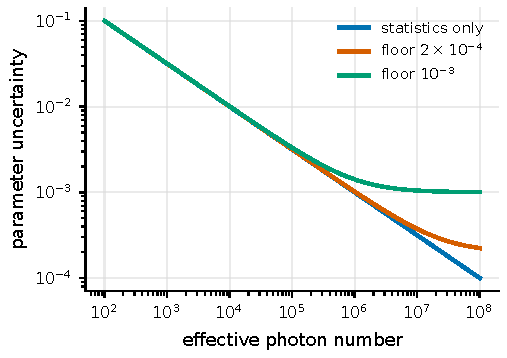
\includegraphics[width=0.70\linewidth]{figures/generated/chapter_07/ch07_fisher_scaling.pdf}
\caption{参数误差随有效光子数的标度。蓝线是纯统计的 \(N_{\rm eff}^{-1/2}\) 沉降；橙、绿线加入不同高度的系统地板后，长时间积分不再改善最终误差。观测计划必须把积分时间、目标亮度、基线覆盖、系统定标放进同一本误差预算里——这正是第 \ref{chap:e15} 章的主题。}
\label{fig:e14-fisher}
\end{figure}

最后提醒：Fisher 矩阵是似然峰附近的局部二次近似，只在高信噪比、后验近高斯时可靠。遇到多峰后验、非线性退化或参数贴边界，就得换 MCMC 或 nested sampling \citep{1925PCPS...22..700F,2013PASP..125..306F,2009MNRAS.398.1601F}。

\section{从相关产品到物理参数}
\label{sec:e14-fit}

有了带协方差的相关产品，最后一步是把物理参数拟合出来。先写\textbf{模型向量}：把角直径、双星分离、亮度比、环半径或喷流参数，映射成各个 \(uv\) 点、各个波长上的平方可见度：
\begin{equation}
  \bm m(\bm\theta)
  =\Big[\,|V(\bm u_1,\lambda_1\mid\bm\theta)|^2,\ \ldots,\ |V(\bm u_{N_d},\lambda_{N_d}\mid\bm\theta)|^2\,\Big] .
  \label{eq:e14-model}
\end{equation}
\begin{formulaexplain}
\(\bm m(\bm\theta)\) 是物理模型预言的数据向量，每项是空间频率 \(\bm u_i\)、波长 \(\lambda_i\) 处的 \(|V|^2\)。它把角直径、双星、结构等参数翻译成可与 \(\bm d\) 直接比较的观测量。
\end{formulaexplain}
这里 \(\bm u=\bm B_\perp/\lambda\) 是空间频率（以波长为单位的投影基线，见第 \ref{chap:e10} 章的 van Cittert–Zernike 定理）。若数据向量 \(\bm d\) 已近似高斯，似然就是带协方差加权的残差：
\begin{equation}
  -2\ln L
  =\big[\bm d-\bm m(\bm\theta)\big]^{T}\Sigma^{-1}\big[\bm d-\bm m(\bm\theta)\big]
   +\ln|\Sigma|+\text{const} .
  \label{eq:e14-gauss}
\end{equation}
\begin{formulaexplain}
\(\bm d-\bm m\) 是数据与模型残差，\(\Sigma^{-1}\) 按协方差加权（相关的点不重复计信息），\(\ln|\Sigma|\) 是归一化项。这是带相关误差的数据产品最常用的高斯似然，最小化它就得到最优参数。
\end{formulaexplain}
注意 \(\Sigma^{-1}\) 那一步正是第 \ref{sec:e14-cov} 节的回报：用完整协方差而不是对角误差，才不会把相关点当成互相独立、把信息量算多。要是直接拟合原始低计数延迟格，就别用高斯，回到式 \eqref{eq:e14-binned-poisson} 的泊松似然。VERITAS-SII 用均匀圆盘和临边昏暗模型拟合 \(|g^{(1)}|^2\) 随投影基线的变化；MAGIC-SII 把 Pearson 相关经通量和背景定标转成 \(|V|^2\) 后拟合角直径与系统误差 \citep{2020NatAs...4.1164A,2024MNRAS.529.4387A,1967MNRAS.137..375H}。

当后验可能多峰、或需要外部先验时，就写成\textbf{贝叶斯后验}：
\begin{equation}
  p(\bm\theta\mid\mathcal D,M)=\frac{L(\mathcal D\mid\bm\theta,M)\,\pi(\bm\theta\mid M)}{Z_M},
  \qquad
  Z_M=\int L\,\pi\,d\bm\theta .
  \label{eq:e14-posterior}
\end{equation}
\begin{formulaexplain}
\(p(\bm\theta\mid\mathcal D,M)\) 是模型 \(M\) 下的参数后验，\(L\) 是似然，\(\pi\) 是先验，\(Z_M\) 是模型证据（归一常数，也用来比较模型）。它把数据约束和外部物理知识合成完整的不确定度。
\end{formulaexplain}
先验 \(\pi\) 可以装距离、光谱型、已知角直径、双星轨道、爆发时间或物理边界——一定要写清楚，因为强度干涉常只测 \(|V|^2\)、缺相位，会让镜像、亮度比、位置角出现退化，是先验帮忙把退化按住。采样上，emcee 适合中等维度后验，MultiNest 适合多峰后验和证据估计 \citep{2013PASP..125..306F,2009MNRAS.398.1601F}；但采样器替代不了物理检查：链的自相关时间、接受率、先验体积、以及"注入已知信号能否无偏恢复"都要一并报告 \citep{1992ApJ...398..146G}。这样一条从事件表到带误差参数的链路才算闭合，第 \ref{chap:e15} 章会把它放进完整的观测设计与可行性评估。

\section{本章要点}
\label{sec:e14-summary}

\begin{itemize}
  \item \textbf{先建模型，再算估计量。}事件表要先写成选择函数式 \eqref{eq:e14-selection} 和泊松似然式 \eqref{eq:e14-point-likelihood}/\eqref{eq:e14-binned-poisson}；点过程似然由"无限窄分箱取极限"自然得到，能保留分箱后丢失的时间信息。
  \item \textbf{相关峰是巨大背景上的微弱超额。}延迟直方图式 \eqref{eq:e14-paircount} 要除以随机符合背景式 \eqref{eq:e14-accidental} 才有意义；真实信号只占背景的 \(10^{-6}\)–\(10^{-4}\)，这从根本上决定了积分时间和定标精度的要求。
  \item \textbf{算得完靠算法，不靠蛮力。}逐对 \(N^2\)/\(N(N-1)/2\) 只配教学；排序窗口式 \eqref{eq:e14-window} 近线性，FFT（XF/FX）随 \(N_{\rm bin}\log N_{\rm bin}\)；台站少时瓶颈在每对吞的时间样本数，GPU/FPGA 实时、无死时间相关把整段涨落都算进去。
  \item \textbf{误差不是独立误差棒。}共享望远镜、背景、定标会让协方差式 \eqref{eq:e14-cov} 出现非对角项；用时间块 bootstrap/jackknife/注入仿真估 \(\Sigma\)，拟合式 \eqref{eq:e14-gauss} 必须用完整 \(\Sigma^{-1}\)。
  \item \textbf{白噪声沉降，系统误差是天花板。}统计误差随 \(N_{\rm eff}^{-1/2}\)、\(T^{-1/2}\) 下降，Fisher 信息随光子数线性、对独立基线相加；但一致性偏移形成不随积分下降的地板，微弱信号把系统容忍度压到同样苛刻的量级。
\end{itemize}

\medskip
\noindent\textbf{想一想。}
(1) 若把延迟格宽 \(\Delta\tau\) 缩小一半，随机符合背景 \(B_{ab,k}\) 和信号超额各怎样变化，最终信噪比是否改善？
(2) 你有 4 台望远镜，为什么"配对数只有 6"并不意味着相关器很轻松？瓶颈在哪个量上？
(3) 一个团队积分时间翻了 10 倍，误差棒却几乎没变小。用本章语言，最可能的诊断是什么？该做哪些空检验去确认？

\chapter{观测设计、误差预算与可行性}
\label{chap:e15}

\begin{chapteropening}
到这里为止，我们已经把工具箱配齐了：第 \ref{chap:e11} 章告诉我们强度干涉的信噪比怎样随望远镜面积、光子率和积分时间标度；第 \ref{chap:e12} 章告诉我们一份数据里到底藏着多少可提取的信息（Fisher 信息与 Cramér--Rao 下界）；第 \ref{chap:e13} 章交代了探测器、时钟和事件表，第 \ref{chap:e14} 章交代了相关器怎样把事件表变成 \(g^{(2)}(\tau)\) 和 \(|V|^2(B)\)。现在要做的，是把这些零件\textbf{攒成一次真实的观测}。想象你面前是一张空白的观测申请表：你要观测哪颗星？用几台望远镜、多长基线、多宽的滤光片？曝多久？最后能把角直径测到百分之几？——这一章就是从头到尾把这张表填满的过程。核心是一张\textbf{账本}：光子率给出统计上限，相关对比度（contrast）给出目标信号，基线、带宽、时间分辨率和定标误差决定这个信号能不能从噪声里活下来。我们会把每一步都算成真实数字，最后走一遍从一颗真实亮星到一个可达精度的完整可行性计算。
\end{chapteropening}

\section{一次观测就是一张从参数到数据的账本}
\label{sec:e15-ledger}

每一次观测，追根究底都是为了估计几个物理数。恒星的角直径、双星的角间距、快速自转星的扁率和长轴方向、谱线发射区的半径、偏振角的旋转、两路信号的时延、二阶相关峰的高度——这些就是我们真正想要的\textbf{物理参数}（physical parameters），记作 \(\bm\theta_{\rm phys}\)。可仪器交给我们的，从来不是这些数，而是第 \ref{chap:e13} 章讲过的\textbf{事件表}（event list）：一行一个光子，带着到达时间、望远镜编号、波长和偏振标签。物理参数要从这些字段里\emph{反推}出来。

于是设计一次观测，第一件事不是问"我想看哪颗星"，而是问"我要的数，事件表里有没有支撑它的字段"。要做纳秒级时间相关，时间戳的精度就得压到纳秒；要给出所需基线，位置标签就得记准；要分波段或测偏振，波长和偏振标签就不能在记录时被抹掉。这里有一条容易被忽视却致命的原则：\textbf{信息一旦在记录环节被平均掉，后期再也补不回来}。如果你一开始只存一张长时间积分的图像，那么纳秒时间相关、偏振相关都已经随平均消失了；而如果你老老实实存下整张事件表，后面就能把它任意投影成光变曲线、\(g^{(2)}(\tau)\)、\(|V|^2(B)\)、偏振角，或者多波长的 \(u,v\) 数据。事件表是"原汤"，图像只是"熬干后的一勺"。

从参数到数据的整条链，可以写成一个似然：

\begin{equation}
  \mathcal L(\bm\theta_{\rm phys})
  =
  P\!\left(\,d \;\middle|\;
  q_{\rm inst}(\bm\theta_{\rm phys}),\;
  \bm c_{\rm cal},\;
  \bm b_{\rm sky}
  \right).
  \label{eq:e15-likelihood}
\end{equation}
\begin{formulaexplain}
\(\bm\theta_{\rm phys}\)：要估计的物理参数（如角直径 \(\theta\)）。\(d\)：观测到的数据或其统计量。\(q_{\rm inst}\)：仪器真正测到的量（如 \(|V|^2\)）。\(\bm c_{\rm cal}\)：定标参数。\(\bm b_{\rm sky}\)：天空背景。这条式子在说：物理参数先被仪器"翻译"成可测量，再和定标、背景一起决定数据出现的概率。
\end{formulaexplain}

逐个符号落地。\(\mathcal L\) 是似然（likelihood），无量纲，衡量"若真参数是 \(\bm\theta_{\rm phys}\)，看到这份数据 \(d\) 的概率有多大"。\(q_{\rm inst}\) 是仪器可测量：可以是平方可见度 \(|V|^2\)（无量纲）、二阶相关的超出量 \(g^{(2)}-1\)（无量纲）、偏振 Stokes 分量，或到达时间残差（秒）。\(\bm c_{\rm cal}\) 是定标参数——时间零点、滤光片通带、探测器效率、增益状态——它们不是我们想要的物理量，却会污染数据，必须一并估计或事先测定。\(\bm b_{\rm sky}\) 是天光、月光、暗计数和宿主星系背景。写观测申请时，与其空泛地说"我们会观测这颗星"，真正有用的是把这条链算穿：这颗星的星等 \(m_B\) 是多少、角直径 \(\theta\) 估计多大、可见窗口有多长、模型先验会给出哪几个 \(|V|^2\) 数据点、最终能把 \(\theta\) 的误差压到百分之几。本章余下几节，就是逐段把这条链填成真实数字。

\section{光子预算：从星等到有效光子数}
\label{sec:e15-photon-budget}

一切从光子率开始。一颗星再有意思，如果每秒只给你几个光子，任何相关信号都会淹没在噪声里。所以可行性计算的第一步，永远是把\textbf{星等翻译成每秒光子数}。这条翻译分四步：星等 \(\to\) 谱流量密度 \(\to\) 单位面积光子通量 \(\to\) 乘上面积与效率得到有效光子率。我们一步一步来。

\paragraph{第一步：星等到谱流量密度}

天文学用星等（magnitude）描述亮度，星等每小 5 等，亮度大 100 倍——这是一把对数尺子。AB 星等的好处是它直接对应谱流量密度：

\begin{equation}
  F_\nu = 3631\,{\rm Jy}\times 10^{-0.4\,m_{\rm AB}}.
  \label{eq:e15-ab-flux}
\end{equation}
\begin{formulaexplain}
\(m_{\rm AB}\)：AB 星等（无量纲）。\(F_\nu\)：单位频率的谱流量密度。\(1\,{\rm Jy}=10^{-23}\,{\rm erg\,s^{-1}\,cm^{-2}\,Hz^{-1}}\)。常数 \(3631\,{\rm Jy}\) 是 \(m_{\rm AB}=0\) 的定义流量。星等每增 5，\(F_\nu\) 降 100 倍。
\end{formulaexplain}

这里 \(F_\nu\) 是谱流量密度，量纲是"能量 / (时间·面积·频率)"，CGS 单位为 \({\rm erg\,s^{-1}\,cm^{-2}\,Hz^{-1}}\)；\(1\,{\rm Jy}\)（央斯基）\(=10^{-23}\) 这个单位。取一颗 \(m_{\rm AB}=5\) 的星，代入即得
\[
  F_\nu = 3631\,{\rm Jy}\times 10^{-0.4\times5}
        = 3631\times10^{-2}\,{\rm Jy}
        = 36.3\,{\rm Jy}
        = 3.63\times10^{-22}\,{\rm erg\,s^{-1}\,cm^{-2}\,Hz^{-1}} .
\]
这就是这颗星在每一赫兹频率上，每秒穿过每平方厘米的能量。数字很小——一平方厘米、一赫兹带宽，一秒钟才收到 \(10^{-22}\) 尔格，这提醒我们后面必须靠大面积和宽带宽把它攒起来。

\paragraph{第二步：能量流量到光子通量}

探测器数的不是能量，是光子个数。一个频率 \(\nu\) 的光子带能量 \(h\nu\)（\(h=6.63\times10^{-27}\,{\rm erg\,s}\) 是普朗克常数）。把能量流量除以单光子能量，就得到单位面积、单位时间、单位带宽的光子数。再乘上光学带宽 \(\Delta\nu\)，就得到整条通带每平方厘米每秒的光子数。带宽换算沿用第 \ref{chap:e02} 章的关系 \(\Delta\nu\simeq c\,\Delta\lambda/\lambda^2\)。取观测波长 \(\lambda=550\,{\rm nm}\)、通带 \(\Delta\lambda=10\,{\rm nm}\)：
\[
  \nu=\frac{c}{\lambda}=\frac{3\times10^{10}\,{\rm cm\,s^{-1}}}{550\times10^{-7}\,{\rm cm}}
     =5.45\times10^{14}\,{\rm Hz},
  \qquad
  h\nu = 6.63\times10^{-27}\times5.45\times10^{14}
       = 3.61\times10^{-12}\,{\rm erg},
\]
\[
  \Delta\nu = \frac{c\,\Delta\lambda}{\lambda^2}
            = \frac{3\times10^{10}\times10\times10^{-7}}{(550\times10^{-7})^2}
            = 9.9\times10^{12}\,{\rm Hz}\approx10^{13}\,{\rm Hz}.
\]
于是单位面积光子通量
\[
  \Phi = \frac{F_\nu\,\Delta\nu}{h\nu}
       = \frac{3.63\times10^{-22}\times 9.9\times10^{12}}{3.61\times10^{-12}}
       \approx 1.0\times10^{3}\ {\rm photons\,s^{-1}\,cm^{-2}} .
\]
一平方厘米、10 nm 通带，每秒约一千个光子——这是\emph{到达大气层顶}的、还没打折的原始通量。

\paragraph{第三步：乘面积与效率，得到有效光子率}

真正落进相关器的光子，还要乘两个因子：望远镜的\textbf{有效收集面积}\(A\)，和从大气到光子计数的\textbf{总效率}\(\eta\)。后者把大气透过率、镜面反射率、滤光片透过率、光纤耦合损失和探测器量子效率（quantum efficiency，见第 \ref{chap:e07} 章）全部并进一个数，典型值 \(\eta\sim0.2\)--\(0.3\)。合起来：

\begin{equation}
  R_\gamma
  = \eta\,A\,\frac{F_\nu\,\Delta\nu}{h\nu}
  = \eta\,A\,\Phi .
  \label{eq:e15-photon-rate}
\end{equation}
\begin{formulaexplain}
\(R_\gamma\)：有效光子率（每秒计数）。\(\eta\)：总效率（无量纲，含大气、镜面、滤光片、探测器）。\(A\)：有效收集面积（\({\rm cm^2}\)）。\(\Phi\)：单位面积光子通量。这条式子把"星有多亮"最终变成"探测器每秒响多少下"。
\end{formulaexplain}

代真实数字。一台口径 12 m 的成像大气切伦科夫望远镜（IACT），收集面积 \(A=\pi(6\,{\rm m})^2\approx113\,{\rm m^2}=1.13\times10^6\,{\rm cm^2}\)。取 \(\eta=0.25\)、\(m_{\rm AB}=5\)：
\[
  R_\gamma = 0.25\times1.13\times10^6\times1.0\times10^3
          \approx 2.8\times10^8\ {\rm s^{-1}} .
\]
每秒约三亿个光子。若这颗星暗到 \(m_{\rm AB}=8\)（比 5 暗 3 等，流量降 \(10^{-1.2}=0.063\) 倍），则 \(R_\gamma\simeq1.8\times10^7\,{\rm s^{-1}}\)。换成 17 m 级口径（如 MAGIC），面积大 2 倍，两种情形分别约 \(5.7\times10^8\) 和 \(3.6\times10^7\,{\rm s^{-1}}\)。这些数字虽大，却\emph{还不是可用的相关事件率}——它们随后还会被空间模式数、偏振、滤光片斜入射、探测器死时间、数据质量切片和背景修正层层削减 \citep{2006ApJ...649..399L,2020MNRAS.491.1540A,2021MNRAS.506.1585Z,2024MNRAS.529.4387A}。图 \ref{fig:e15-photon-rate} 把这条星等到光子率的曲线画了出来。

\begin{figure}[tbp]
\centering
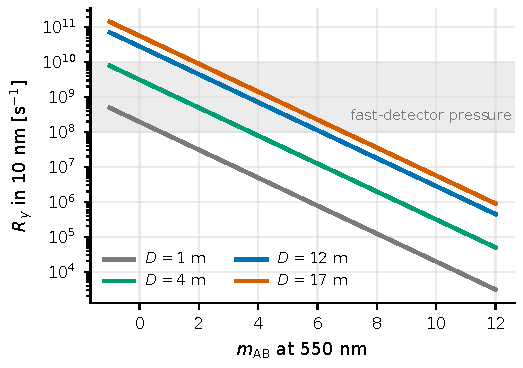
\includegraphics[width=0.86\linewidth]{figures/generated/chapter_18/ch18_photon_rate_magnitude.pdf}
\caption{AB 星等到窄带光子率的换算。曲线采用 550 nm、10 nm 通带、总效率 \(\eta=0.25\)。口径只线性改变收集面积，星等每增 5 等会让光子率降 100 倍；灰色区域标出 \(10^8\,{\rm s^{-1}}\) 以上、开始对高速探测和数据吞吐形成压力的区间。}
\label{fig:e15-photon-rate}
\end{figure}

\paragraph{相干稀释：为什么原始光子率不等于可用信号}

强度干涉真正要测的，是二阶相关在零延迟处的那个小小凸起，它的高度由光学\textbf{相干时间}\(\tau_c\)（coherence time，第 \ref{chap:e02} 章）和电子响应时间共同决定。相干时间是"光波还记得自己相位的时间"，由带宽定：\(\tau_c\simeq1/\Delta\nu\simeq\lambda^2/(c\,\Delta\lambda)\)。取 VERITAS 常用的 416 nm、13 nm 通带：
\[
  \tau_c\simeq\frac{\lambda^2}{c\,\Delta\lambda}
  =\frac{(416\times10^{-7})^2}{3\times10^{10}\times13\times10^{-7}}
  \approx 4.4\times10^{-14}\,{\rm s} .
\]
这是几十飞秒——比任何电子学快得多。而探测器加电子链的等效时间宽度是 \(\Delta t\sim4\,{\rm ns}\)。真正的相关峰只在 \(\tau_c\) 这么窄的时间里成立，却被摊平到 \(\Delta t\) 这么宽的时间 bin 里，于是峰高被稀释了约 \(\tau_c/\Delta t\)：
\[
  \frac{\tau_c}{\Delta t}\approx\frac{4.4\times10^{-14}}{4\times10^{-9}}
  \approx1.1\times10^{-5}.
\]
所以未解析热光在零基线上的归一化相关峰，自然落到几个 \(10^{-6}\) 的量级——这正是 VERITAS 论文里测到的 \(N_0\sim10^{-6}\) 那一档 \citep{2020NatAs...4.1164A,2024ApJ...966...28A}。峰这么矮，意味着它必须靠长时间平均和严格定标才能从噪声里"浮"出来。图 \ref{fig:e15-coherence} 把这层稀释画了出来。

\begin{figure}[tbp]
\centering
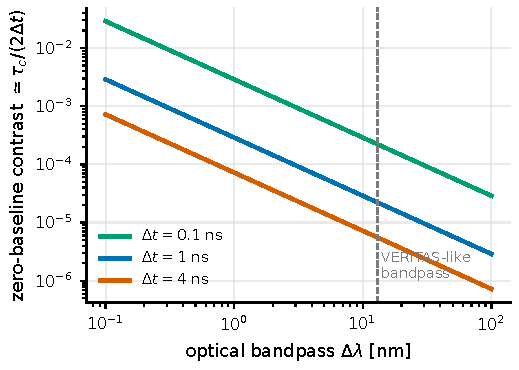
\includegraphics[width=0.86\linewidth]{figures/generated/chapter_18/ch18_coherence_dilution.pdf}
\caption{通带越宽，光学相干时间越短；电子时间分辨率越慢，零延迟相关峰越被稀释。416 nm、13 nm、4 ns 的组合给出几个 \(10^{-6}\) 的对比度，因此相关峰只能靠长积分和严格定标从噪声中显形。}
\label{fig:e15-coherence}
\end{figure}

这里藏着一个反直觉但极重要的事实：\textbf{把光学通带调宽，并不会按比例改善信噪比}。宽带确实让光子多了（\(R_\gamma\propto\Delta\lambda\)），但同时把相干时间缩短、把每个时间 bin 里的相关对比度压低（\(\propto\tau_c\propto1/\Delta\lambda\)）。两者在信噪比里几乎恰好抵消——下一节会看到这一点。真实仪器仍要挑滤光片，但那是为了控制 PMT 电流、天空背景、斜入射效应或选谱线，而不是简单地"越宽越好" \citep{2020MNRAS.491.1540A,2024MNRAS.529.4387A}。

\section{信噪比与积分时间怎么估}
\label{sec:e15-snr}

有了光子率，就能问最关心的问题：曝多久，信号才够强？第 \ref{chap:e11} 章推出的强度干涉信噪比标度是这一切的核心：

\begin{equation}
  {\rm SNR}
  = A\,\alpha\,n\,|V(\bm B)|^2\,
    \sqrt{\frac{\Delta f\,T}{2}} .
  \label{eq:e15-snr}
\end{equation}
\begin{formulaexplain}
\(A\)：收集面积（\({\rm cm^2}\)）。\(\alpha\)：量子效率（无量纲）。\(n\)：入射谱光子密度 \({\rm photons\,s^{-1}\,cm^{-2}\,Hz^{-1}}\)。\(|V|^2\)：平方可见度。\(\Delta f\)：电子带宽（Hz）。\(T\)：积分时间（s）。信号随 \(\sqrt{T}\) 攒起来。
\end{formulaexplain}

先把每个符号钉牢。\(A\) 是每台望远镜的有效面积（\({\rm cm^2}\)）；\(\alpha\) 是量子效率（无量纲）；\(n\) 是\textbf{入射谱光子密度}——单位面积、单位时间、单位光学带宽里的光子数，量纲 \({\rm photons\,s^{-1}\,cm^{-2}\,Hz^{-1}}\)，它由源的表面亮度（也就是亮温）决定，\emph{与你选多宽的光学通带无关}。\(|V(\bm B)|^2\) 是基线 \(\bm B\) 上的平方可见度（无量纲，介于 0 与 1），是我们真正想测的目标信号。\(\Delta f\) 是电子带宽（Hz），由光脉冲、PMT/SPAD 响应、线缆、放大器、数字化器和软件相关共同决定的等效带宽。\(T\) 是积分时间（s）。

这条式子有几处值得咀嚼。第一，把 \(A\,\alpha\,n\) 合起来看：它的量纲是 \({\rm s^{-1}\,Hz^{-1}}\)，而 \({\rm Hz^{-1}=s}\)，所以整体\emph{无量纲}——它就是每个模式里的平均光子占据数 \(\delta=A\alpha n\)，即\textbf{光子简并度}（photon degeneracy）。可见光热星的 \(\delta\) 只有 \(10^{-4}\)--\(10^{-2}\)，这正是强度干涉信号如此微弱的根源。第二，因为 \(n\) 是\emph{谱}密度，加宽光学通带并不改 \(n\)——这就从公式上证实了上一节那句"宽带不白赚信噪比"。第三，也是最实用的一条：\({\rm SNR}\propto\sqrt{T}\)。信号不是线性攒的，是\emph{开方}攒的——要把信噪比翻倍，得曝四倍长的时间。这条 \(\sqrt{T}\) 定律下一节会成为误差预算的主角。

代一个真实场景。LeBohec 与 Holder 取 \(A=100\,{\rm m^2}\)、\(\alpha=0.3\)、\(\Delta f=1\,{\rm GHz}\)、\(T=5\,{\rm h}=1.8\times10^4\,{\rm s}\)、\(|V|^2=0.5\)，算得一颗 \(m_V\simeq6.7\) 的星恰好落在 \(5\sigma\) 一档；同样条件下 \(m_V=5\) 的星（亮 1.7 等、\(n\) 大约 5 倍）信噪比冲到二十以上，而 \(m_V=9\) 的星只剩不到 \(1\sigma\)，等于测不出 \citep{2006ApJ...649..399L,2008AIPC..984..205L}。把这套依赖画成星等\,--\,积分时间的热图，就是图 \ref{fig:e15-snr}。要反过来求积分时间也很直接：把式 \eqref{eq:e15-snr} 解出 \(T\)，
\[
  T = \frac{2\,{\rm SNR}^2}{(A\alpha n)^2\,|V|^4\,\Delta f},
\]
即所需时间随目标信噪比\emph{平方}增长、随简并度平方和可见度四次方\emph{反比}下降——这解释了为什么暗一点、或已被高度解析（\(|V|^2\) 很小）的目标，会让积分时间迅速失控。

\begin{figure}[tbp]
\centering
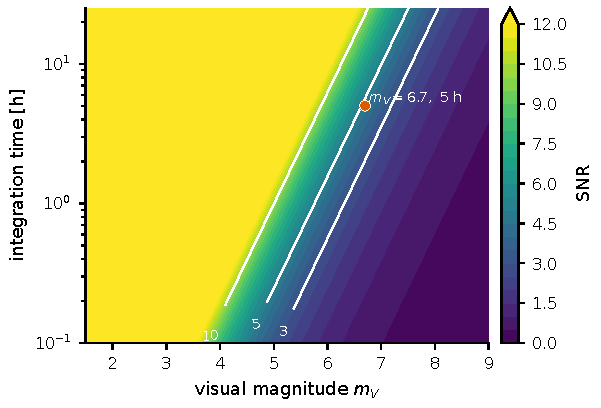
\includegraphics[width=0.90\linewidth]{figures/generated/chapter_18/ch18_snr_heatmap.pdf}
\caption{强度干涉信噪比对星等和积分时间的依赖。图中取 \(A=100\,{\rm m^2}\)、\(\alpha=0.3\)、\(\Delta f=1\,{\rm GHz}\)、\(|V|^2=0.5\)；橙点对应 LeBohec--Holder 估算里 \(m_V\simeq6.7\)、5 h 约 \(5\sigma\) 的位置。}
\label{fig:e15-snr}
\end{figure}

用式 \eqref{eq:e15-snr} 做第一轮估算时要记住它是"理想版"。真实数据里，\(T\) 是过了质量切片后的有效曝光时间（live time），不是挂钟时间；\(\Delta f\) 是整条电子链的等效带宽；\(|V|^2\) 还会随目标高度和时角缓慢变化。举一组真实工程数字：VERITAS 用四台 12 m 望远镜同时给出六条基线，配 416 nm、约 13 nm 滤光片和 4 ns 采样，每小时吐出约 3.5 TB 原始数据；MAGIC 用两台 17 m 望远镜和中央 PMT，早期演示报告的灵敏度比 Narrabri 高约一个量级。而 Vega 光子计数实验走的是另一条路——用单光子雪崩二极管（SPAD）加软件相关，在零基线测到 \(\langle g^{(2)}\rangle=1.0034\pm0.0008\)，在约 2 km 投影基线上则\emph{不}出现相关，正符合 Vega 约 3.3 mas 的角直径在那条基线上已被完全解析的预期 \citep{2020NatAs...4.1164A,2020MNRAS.491.1540A,2021MNRAS.506.1585Z}。

多台望远镜同时买到两样东西：更多数据、更多几何。\(N\) 台望远镜给出 \(N(N-1)/2\) 条同时基线——4 台只有 6 条，60 台就有 1770 条。关键是，不同基线是在 \(u,v\) 平面的\emph{不同点}上采样源结构，绝非重复测量同一个数（第 \ref{chap:e11} 章）。测均匀圆盘直径，几条合适基线就够；但要测快速自转星的扁率、双星、盘风或非轴对称的谱线发射区，就非要位置角覆盖不可。覆盖 0.1--3 mas 的热星结构时，30--2000 m 这一整段基线范围，比单纯堆一条最长基线更有用。图 \ref{fig:e15-uv} 对比了小阵列与大阵列的 \(u,v\) 覆盖。

\begin{figure}[tbp]
\centering
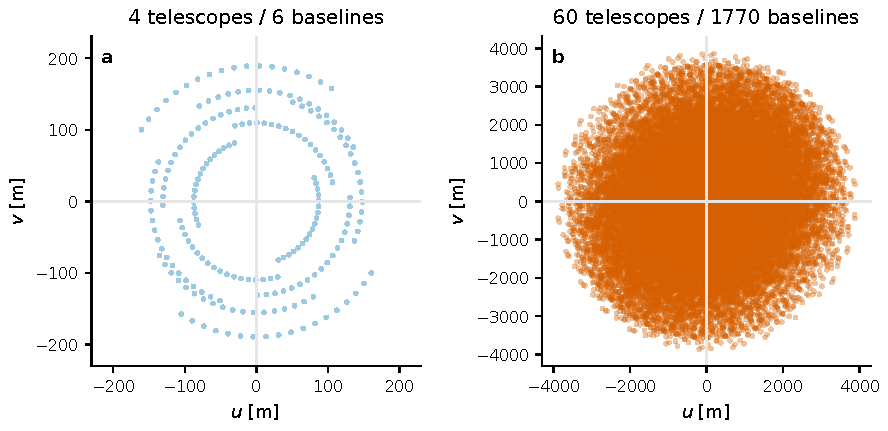
\includegraphics[width=0.94\linewidth]{figures/generated/chapter_18/ch18_uv_coverage.pdf}
\caption{阵列规模怎样改变 \(u,v\) 采样。左：四台望远镜的六条基线，随时角旋转后仍较稀疏；右：多望远镜阵列，短、中、长基线同时存在。密集覆盖不自动等于高信噪比，但它决定非轴对称目标能否被稳定拟合或重建。}
\label{fig:e15-uv}
\end{figure}

\section{基线、带宽与波段的选择由可见度斜率决定}
\label{sec:e15-baseline}

已经有了信噪比，为什么还不能马上定基线？因为\textbf{信号强}和\textbf{信息多}是两回事。一条基线可能相关峰很高（信噪比很好），却对我们想测的角直径几乎不敏感——这时它测得再准也没用。要判断"哪条基线才携带直径信息"，得看可见度曲线的\emph{斜率}。

先把角尺度和基线的粗关系摆出来。要分辨角尺度 \(\theta\)，需要的基线约为

\begin{equation}
  B\sim\frac{\lambda}{\theta}
  = 86\,{\rm m}\left(\frac{\lambda}{416\,{\rm nm}}\right)
                \left(\frac{1\,{\rm mas}}{\theta}\right).
  \label{eq:e15-baseline}
\end{equation}
\begin{formulaexplain}
\(B\)：所需基线（m）。\(\lambda\)：观测波长。\(\theta\)：目标角尺度（这里以 mas 为单位）。这是量级式：要分辨越小的角，需要越长的基线；波长越短，同样基线分辨越细。
\end{formulaexplain}

代几个数就有画面了：\(\theta=2\,{\rm mas}\) 的热星在 416 nm 只要约 43 m 就开始被解析；\(\theta=0.5\,{\rm mas}\) 要约 170 m；\(\theta=0.1\,{\rm mas}\) 得进到约 860 m。Narrabri 的最大基线约 188 m，所以它最擅长又亮又热、角直径在零点几到几 mas 的星；CTA 级的公里阵列能把空间频率推到几十微角秒，但目标还得有足够光子率才玩得起 \citep{1974MNRAS.167..121H,2006ApJ...649..399L}。

现在看斜率。均匀圆盘（第 \ref{chap:e11} 章）的平方可见度随基线先是接近 1 的平台，然后下降，在第一零点处触底。观测设计的要害在于：如果你所有基线都落在 \(|V|^2\simeq1\) 的平台上，不同 \(\theta\) 的曲线几乎重合，你根本分不出星的大小；如果你只测第一零点\emph{之后}的极低可见度，相关峰又低到贴着噪声。\textbf{直径信息集中在曲线下降最陡、也就是斜率 \(|\partial|V|^2/\partial\theta|\) 最大的那一段基线}——通常在第一 lobe 的下降区和第一零点附近。所以一份严肃的可行性计算，不但要画目标模型的 \(|V|^2(B)\)，还要画它对参数的导数 \(\partial|V|^2/\partial\theta\)，看峰值落在哪条基线（图 \ref{fig:e15-vis}）。

\begin{figure}[tbp]
\centering
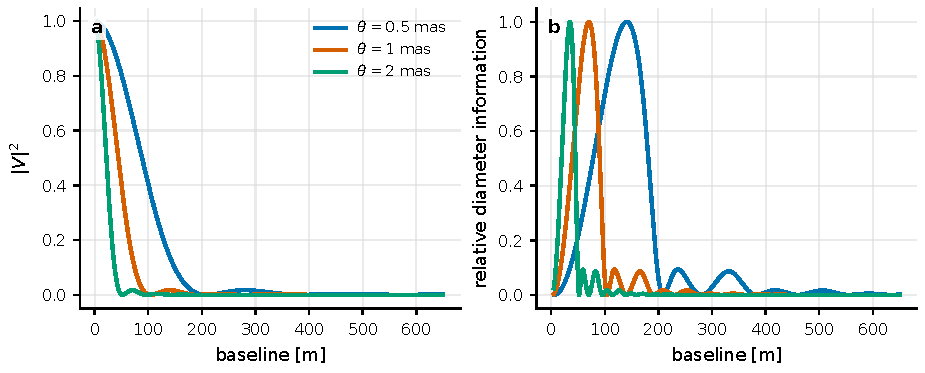
\includegraphics[width=0.94\linewidth]{figures/generated/chapter_18/ch18_visibility_fisher.pdf}
\caption{均匀圆盘的平方可见度曲线与直径灵敏度。416 nm 下，2 mas、1 mas、0.5 mas 目标的下降区分别落在几十米、百米、几百米基线；右图显示直径信息主要来自曲线斜率大的基线，短基线平台 \(|V|^2\simeq1\) 对直径几乎不敏感。}
\label{fig:e15-vis}
\end{figure}

把这层直觉写成公式，就是第 \ref{chap:e12} 章的 Fisher 信息。对单个参数 \(\theta\)、一组独立基线测量 \(\mu_i=|V_i|^2\)，Fisher 信息与可达方差为

\begin{equation}
  I(\theta)=\sum_i
  \frac{1}{\sigma_i^2}
  \left(\frac{\partial\mu_i}{\partial\theta}\right)^{\!2},
  \qquad
  \sigma_\theta\ge\frac{1}{\sqrt{I(\theta)}} .
  \label{eq:e15-fisher}
\end{equation}
\begin{formulaexplain}
\(\mu_i\)：第 \(i\) 条基线上的可测量（如 \(|V_i|^2\)）。\(\partial\mu_i/\partial\theta\)：它对目标参数的灵敏度（斜率）。\(\sigma_i\)：该测量的误差。右式是 Cramér--Rao 下界。斜率大、误差小的基线，贡献最大。
\end{formulaexplain}

这条式子把前面几句话变成了可算的判据。每条基线的贡献是\emph{斜率平方除以误差平方}：斜率 \(\partial\mu_i/\partial\theta\) 大、误差 \(\sigma_i\) 小，才贡献得多。于是两种"看着不错却没用"的基线立刻现形——误差再小、但斜率近零（平台上）的基线，贡献几乎为零；斜率再大、但 \(|V|^2\) 太低导致相关峰淹在噪声里、\(\sigma_i\) 巨大的基线，也撑不起结果。注意 \(\sigma_i\) 里既要放统计噪声（来自式 \eqref{eq:e15-snr}），也要放下一节的系统项。VERITAS 对快速自转星 \(\gamma\) Cas 的观测就是活例子：不同投影基线采样不同方向的 \(|V|^2\)，才约束出扁率和长轴方向，单一个等效圆盘直径根本描述不了这种非轴对称目标 \citep{2025ApJ...995..191A,2024ApJ...966...28A}。

波段选择跟着一起决定。同一条物理基线，在 416 nm 采到的空间频率比 800 nm 高约 1.9 倍——蓝端分辨率更高，但大气透过、镜面反射、探测器量子效率和滤光片斜入射都更难对付。谱线观测则要换一套账：算的是线通量而非宽带星等。对热星和 Be 星，H\(\alpha\)、氦线或金属线可能来自比连续谱更大的发射区；用窄带把几何结构和速度通道分开是值得的，但每个通道的事件率、滤光片泄漏和背景都得重新算过 \citep{2012NewAR..56..143D,2021MNRAS.506.1585Z}。

\section{误差预算：统计地板与系统地板}
\label{sec:e15-error-budget}

现在到了整章最实用、也最容易被外行忽略的一节。新手写观测申请，往往只报一个信噪比就完事。但信噪比只管\emph{统计}噪声，它会随积分时间一路下降；真正决定"你到底能测多准"的，常常是一层\textbf{不随时间下降的系统地板}。把两者分开，就是误差预算。

对一个待拟合参数 \(\theta\)，把各路误差按方差相加：

\begin{equation}
  \sigma_\theta^2
  = \sigma_{\rm stat}^2
  + \sigma_{\rm bg}^2
  + \sigma_{\rm time}^2
  + \sigma_{\rm cal}^2
  + \sigma_{\rm model}^2 .
  \label{eq:e15-error-budget}
\end{equation}
\begin{formulaexplain}
\(\sigma_\theta\)：目标参数的总误差。右边依次是统计、背景、时间、定标、模型误差。它们独立时按方差相加。这条式子提醒你：报一个信噪比不够，还得说清误差平台从哪来。
\end{formulaexplain}

逐项说清它们各是什么、量纲都折算到 \(\theta\) 的单位上。\(\sigma_{\rm stat}\) 来自有限的符合计数或相关峰拟合，是式 \eqref{eq:e15-snr} 那个信噪比的直接后果。\(\sigma_{\rm bg}\) 来自离源背景（off-source）插值和暗电流的不确定。\(\sigma_{\rm time}\) 来自时钟、几何延迟、采样和峰形。\(\sigma_{\rm cal}\) 来自校准星、系统总透过率、滤光片和偏振。\(\sigma_{\rm model}\) 来自源模型本身——把快速自转星硬当成圆盘、把谱线盘硬当成高斯、或忽略一颗伴星，都会引入这项。

关键的物理在于它们\emph{随时间的行为不同}。统计项遵守散粒噪声的 \(\sqrt N\) 定律（第 \ref{chap:e03} 章）：计数 \(N\propto T\)，所以

\begin{equation}
  \sigma_{\rm stat}(T)=\frac{c_0}{\sqrt{T}} ,
  \qquad
  \sigma_{\rm sys}^2=\sigma_{\rm bg}^2+\sigma_{\rm time}^2
        +\sigma_{\rm cal}^2+\sigma_{\rm model}^2 ,
  \label{eq:e15-floor}
\end{equation}
\begin{formulaexplain}
\(c_0\)：由光子率、可见度斜率等决定的常数。\(\sigma_{\rm stat}\propto T^{-1/2}\) 随曝光下降；\(\sigma_{\rm sys}\) 把不随时间下降的系统项合在一起。总误差是两者的方差和。
\end{formulaexplain}

这里 \(c_0\) 是把光子率、可见度斜率、定标链一并吸收进去的常数（单位与 \(\theta\) 一致）。图像很清楚：\(\sigma_{\rm stat}\) 像一条不断下滑的斜坡，随你曝得越久越低；而 \(\sigma_{\rm sys}\) 是一块\emph{水平的地板}。总误差是二者的方差和，一开始被统计斜坡主导、随 \(T\) 下降，直到撞上系统地板就\emph{不动了}。撞上的时刻，就是统计项等于系统项的那一刻：
\[
  \sigma_{\rm stat}(T_\star)=\sigma_{\rm sys}
  \;\Longrightarrow\;
  T_\star=\left(\frac{c_0}{\sigma_{\rm sys}}\right)^{2}.
\]
\textbf{曝到 \(T_\star\) 以后再加时间，几乎白费}——总误差已经贴着系统地板，你把 \(T\) 再翻四倍，统计项才减半，而它早已远小于地板，对总误差毫无影响。这就是可行性计算里最该讲清、也最该写进申请的一句话：不是"曝得越久越好"，而是"曝到统计项降到系统地板附近就该停，剩下的精度要靠压低系统项去争"。图 \ref{fig:e15-budget} 把这条斜坡撞地板的行为画了出来。

\begin{figure}[tbp]
\centering
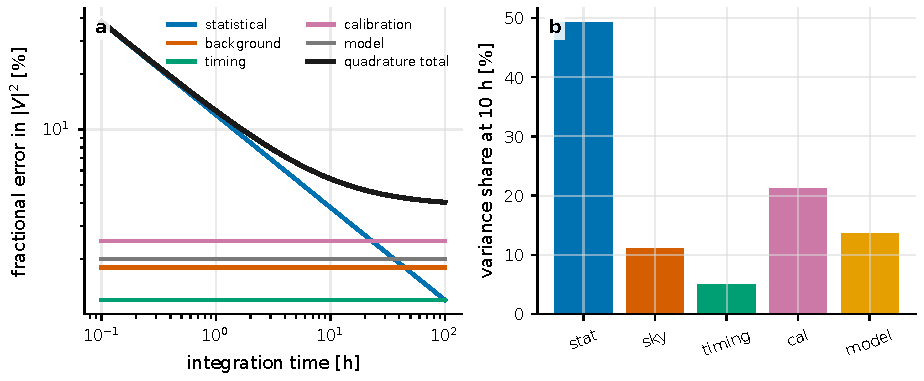
\includegraphics[width=0.94\linewidth]{figures/generated/chapter_18/ch18_error_budget.pdf}
\caption{误差预算里的统计项与系统项。左：统计误差随积分时间下降，但背景、时间、定标、模型项合成一块平台；右：10 h 时各项对总方差的贡献。观测申请应把每一项都连到一份可观测的定标数据，并在总信噪比之外给出误差平台。}
\label{fig:e15-budget}
\end{figure}

系统项里最常见、也最好量化的一项是\textbf{背景稀释}。若源外还有一份与信号\emph{不相关}的背景光（天光、月光、暗计数），它不会造出假相关，却会把真相关峰按比例压低。设某端背景与星光之比为 \(\beta\)，两端对称时观测到的对比度按 \((1+\beta)^{-2}\) 缩水（第 \ref{chap:e08} 章）。代数字：\(\beta=0.03\)（背景只有星光的 3\%）时 \((1.03)^{-2}=0.94\)，只掉 6\%，几乎无害；但 \(\beta=0.5\) 时 \((1.5)^{-2}=0.44\)，峰只剩原来的四成多。VERITAS 对 \(\beta\) UMa 的分析，用目标附近 0.5\(^\circ\) 的离源观测（off runs）估非星光电流，典型离源强度只有在源的约 3\%，所以对半径拟合影响很小；可一旦有明月、云、雾、城市灯光或探测器后脉冲（afterpulsing），这个近似就变差，得单独做质量切片 \citep{2024ApJ...966...28A,2025ApJ...995..191A}。图 \ref{fig:e15-bg} 给出稀释因子及其反向修正。

\begin{figure}[tbp]
\centering
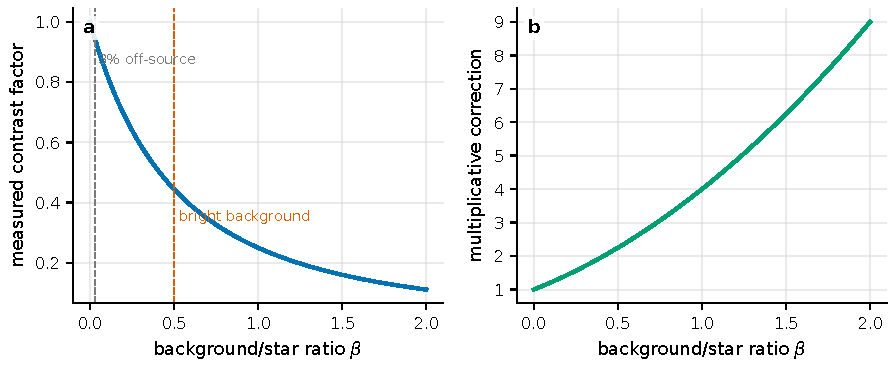
\includegraphics[width=0.94\linewidth]{figures/generated/chapter_18/ch18_background_dilution.pdf}
\caption{不相关背景对相关峰的稀释。两端背景/星光比相同时，观测对比度按 \((1+\beta)^{-2}\) 下降：\(\beta=0.03\) 只造成几个百分点修正，\(\beta=0.5\) 已把峰压到约 44\%。右图是反向修正因子，修正越大，对背景估计误差越敏感。}
\label{fig:e15-bg}
\end{figure}

时间定标是强度干涉和光子计数共同的硬边界。相关峰宽通常几纳秒；若两台望远镜的相对延迟模型错了 1 ns，峰就会被摊宽、甚至移出拟合窗口。Vega 光子计数实验里，零基线子孔径的相对时间精度约 100 ps，两台望远镜之间还要处理光行时、仪器延迟、GPS 或铷钟漂移和光纤色散，最后用约 400 ps 的时间 bin 做相关；他们明确指出多望远镜方案要做到约纳秒级同步，才能把观测时间维持在小时量级。VERITAS 用 White Rabbit 的 10 MHz 时钟分发加 4 ns 采样，仍要在每个 run 里跟踪光程延迟随时角的漂移，并处理 run 到 run 的峰位变化 \citep{2021MNRAS.506.1585Z,2024ApJ...966...28A}。

校准星（calibrator）要跟科学目标一样认真选。理想的校准星应有已知角直径、稳定光度、贴近目标的天区位置、相近颜色和足够高的光子率。若目标是 0.5 mas 的热星，而校准星直径本身有 5\% 的不确定，那么最终直径误差很容易被这一项 \(\sigma_{\rm cal}\) 主导——曝再久也没用。现代强度干涉观测常先拿已知角直径的热星当参考，核对零基线归一化、滤光片响应和 \(|V|^2(B)\) 形状，再去测未知目标。MAGIC 2024 年的性能论文就用多颗参考星验证系统，再给出新恒星角直径；VERITAS 从 \(\beta\) UMa 的圆盘直径一路走到 \(\gamma\) Cas 的扁率和位置角，用的也是同一套定标框架 \citep{2024MNRAS.529.4387A,2024ApJ...966...28A,2025ApJ...995..191A}。

\section{一次从头到尾的可行性计算}
\label{sec:e15-worked}

现在把整章串成一次真实的算。设科学目标是：\textbf{用 VERITAS 型阵列测量一颗热亮星的角直径，把相对误差压到百分之几}。阵列参数全部取自真实的 VERITAS 强度干涉系统；目标取一颗落在灵敏度边缘的热星，好让这道题既不是"轻松能测"也不是"根本没戏"。

\textbf{第 0 步：写下目标参数与成功标准。}要测的物理量是角直径 \(\theta\)，目标精度 \(\sigma_\theta/\theta\lesssim3\%\)。成功标准量化为：至少三条基线在第一 lobe 下降区达到 \({\rm SNR}>5\)；校准星重复观测的归一化漂移小于 3\%；离源背景修正小于总信号的 10\%。

\textbf{第 1 步：选目标，定光子率。}我们特意挑一颗比 \(\beta\) UMa（\(m_V\approx2.4\)）、\(\gamma\) Cas（\(m_V\approx2.2\)）这些 VERITAS 真实亮目标更暗、正落在灵敏度边缘的 \(m_V\approx5\) 假想早型星，有效温度约 \(10^4\,{\rm K}\)，好让这道题不至于太轻松。（提醒一句：本节用到的 \(m_V\approx5\)、\(T_{\rm eff}\approx10^4\,{\rm K}\)、\(\theta\approx0.7\,{\rm mas}\) 是为演示各步骤而\emph{各自独立给定}的示意数，不必对应同一颗真实恒星——若认真代进 Stefan--Boltzmann 关系 \(f_{\rm bol}=\sigma T^4(\theta/2)^2\)，会发现这三个数并不严格自洽，读者不必纠结于此。）用第 \ref{sec:e15-photon-budget} 节的链条，一台 12 m 望远镜在 550 nm、10 nm 通带、\(\eta=0.25\) 下给出 \(R_\gamma\simeq2.8\times10^8\,{\rm s^{-1}}\)。换到 VERITAS 实际的 416 nm、13 nm 滤光片，光子率同量级。结论：光子够多，这颗星不会因为太暗而出局。

\textbf{第 2 步：估角尺度，定基线。}\(10^4\,{\rm K}\) 的早型亮星角直径通常在 0.5--1 mas。由式 \eqref{eq:e15-baseline}，在 416 nm 下 \(\theta\approx0.7\,{\rm mas}\) 的星，第一 lobe 下降区落在约 \(86/0.7\approx120\,{\rm m}\) 一带。VERITAS 四台 12 m 望远镜的六条基线覆盖几十米到约 170 m，正好把下降区和第一零点附近都罩住——这意味着我们有几条基线落在\emph{斜率大}的位置上，符合第 \ref{sec:e15-baseline} 节的直径信息判据。

\textbf{第 3 步：估相关峰高与统计信噪比。}由第 \ref{sec:e15-photon-budget} 节，416 nm、13 nm、4 ns 给出 \(\tau_c\simeq4.4\times10^{-14}\,{\rm s}\)、稀释后的零基线峰约几个 \(10^{-6}\)。把阵列参数代入式 \eqref{eq:e15-snr}：LeBohec--Holder 的等效计算表明，\(A=100\,{\rm m^2}\)、\(\alpha=0.3\)、\(\Delta f=1\,{\rm GHz}\)、\(|V|^2=0.5\) 时，\(m_V\simeq6.7\) 的星 5 h 达到 \(5\sigma\)；我们这颗 \(m_V\approx5\) 的星亮约 5 倍，同样 5 h 的单基线信噪比可冲到二十以上。取保守的单基线 \({\rm SNR}\approx5\)--\(10\) 已足够。

\textbf{第 4 步：把信噪比翻译成角直径误差。}相关峰的相对误差是 \(\sigma_{|V|^2}/|V|^2\approx1/{\rm SNR}\)。要把它换成角直径的误差，用一次\textbf{误差传播}（error propagation）：可测量 \(|V|^2\) 是 \(\theta\) 的函数，\(\theta\) 的小误差经导数搬运成 \(|V|^2\) 的误差，
\[
  \sigma_{|V|^2}=\left|\frac{\partial|V|^2}{\partial\theta}\right|\,\sigma_\theta .
\]
把这条式子两边同时除以 \(|V|^2\) 与 \(\theta\)，右边正好凑成对数导数 \(\partial\ln|V|^2/\partial\ln\theta=(\theta/|V|^2)\,\partial|V|^2/\partial\theta\)，于是
\[
  \frac{\sigma_\theta}{\theta}
  =\frac{\sigma_{|V|^2}/|V|^2}{\left|\partial\ln|V|^2/\partial\ln\theta\right|} .
\]
在下降区，可见度对直径的\emph{对数斜率}\(|\partial\ln|V|^2/\partial\ln\theta|\) 是 1--2 量级；代入 \(\sigma_{|V|^2}/|V|^2\approx1/{\rm SNR}\)，得
\[
  \frac{\sigma_\theta}{\theta}
  \approx\frac{1}{{\rm SNR}}\,
  \frac{1}{\left|\partial\ln|V|^2/\partial\ln\theta\right|}
  \approx\frac{1}{5}\times\frac{1}{1.5}
  \approx13\%
\]
——\emph{单条}斜率大的基线，5 h 大约给到十几个百分点。再用式 \eqref{eq:e15-fisher} 把多条基线的信息相加：\(N_b\) 条同等有用的基线让统计误差按 \(1/\sqrt{N_b}\) 缩小，六条基线里若有三条落在下降区，\(\sigma_\theta/\theta\) 就压到约 \(13\%/\sqrt3\approx7\%\)；再叠几个夜晚或用更多台望远镜的更多基线，进到 3\% 是现实的。这一步把"信噪比"真正落成了"角直径能测到百分之几"。

\textbf{第 5 步：核对误差预算，判断该不该继续曝。}用式 \eqref{eq:e15-error-budget} 和 \eqref{eq:e15-floor} 检查系统地板。背景：离源 \(\beta\approx0.03\)，稀释修正约 6\%，且可由离源观测标定，\(\sigma_{\rm bg}\) 小。时间：White Rabbit 加 4 ns 采样，相对延迟控制在纳秒级，\(\sigma_{\rm time}\) 可控。定标：若校准星直径已知到 3\%，则 \(\sigma_{\rm cal}\) 约 3\%——这恰好和我们的目标精度同量级，成为\textbf{最可能的系统地板}。据式 \eqref{eq:e15-floor}，当统计项 \(\sigma_{\rm stat}\) 曝到降至约 3\% 时（对应 \(T_\star\)），总误差就贴着这块由校准星决定的地板，\emph{再加曝光已无意义}。结论直白：这次观测能否达到 3\%，最后不取决于再曝几小时，而取决于\emph{有没有一颗直径足够确定的校准星}。

\textbf{第 6 步：写成申请里的可行性结论。}一句话收束：目标 \(m_V\approx5\)、\(\theta\approx0.7\,{\rm mas}\) 的热星，用 VERITAS 六条基线、416 nm/13 nm、4 ns 采样，数个夜晚的有效曝光可在下降区多条基线上达到 \({\rm SNR}>5\)，把角直径统计误差压到约 3\%；系统地板由校准星直径不确定（约 3\%）主导，因此升级方向不是更长曝光，而是更好的校准星与更严的滤光片/背景控制。若最长基线未检出相关，仍能给出角直径\emph{上限}或排除过大的发射区——空手而归也是有价值的结果。

这条估算链并不专属强度干涉。振幅干涉、量子网络望远镜、CMB 偏振、快速射电暴（FRB）的光子统计，乃至实验室教学台架，都套同一副骨架：事件率 \(\to\) 模式数 \(\to\) 响应函数 \(\to\) 定标项 \(\to\) 模型导数 \(\to\) 误差预算；差别只在可测量 \(\mu_i\) 的具体形式。科学案例排序也该沿用这条思路，把"科学价值"和"可观测性"分成两栏各自打分，别把\emph{漂亮的}目标和\emph{做得成的}目标混为一谈 \citep{2010SPIE.7734E..0AD,2012MNRAS.419..172N,2013APh....43..331D,2022SPIE12183E..0DK}。表 \ref{tab:e15-checklist} 把这份账本里每个量的常见范围和用法列成一张清单。

\begin{longtable}{p{0.16\linewidth}p{0.30\linewidth}p{0.44\linewidth}}
\caption{可行性账本速查表：每个量的常见范围与在计划中的用法。}
\label{tab:e15-checklist}\\
\toprule
量 & 常见范围 & 在计划中的用法 \\
\midrule
\endfirsthead
\toprule
量 & 常见范围 & 在计划中的用法 \\
\midrule
\endhead
\(m_V,\,m_B\) & \(-1\) 到 \(9\) 等，是当前强度干涉的主战场 & 经式 \eqref{eq:e15-ab-flux} 与 \eqref{eq:e15-photon-rate} 转成 \(R_\gamma\)，先判断目标是否过暗。 \\
\(A_{\rm eff}\) & 每台 \(1\)--\(250\,{\rm m^2}\) & 进入光子率与信噪比；镜面老化、遮挡、光纤耦合都要折进效率。 \\
\(\Delta\lambda\) & \(0.1\)--\(30\,{\rm nm}\) & 决定相干时间、PMT 电流、天空背景与谱线选择。 \\
\(\Delta t\) & \(0.1\)--\(5\,{\rm ns}\) & 决定相关峰被稀释的程度和可用电子带宽。 \\
\(B_p\) & \(10\)--\(2000\,{\rm m}\) & 决定角尺度和 \(u,v\) 覆盖；短、长基线约束不同结构。 \\
\(\beta\) & \(0.01\)--\(1\) & 背景/星光比，决定对比度稀释与背景系统误差。 \\
\(\sigma_{\rm cal}\) & 可见度或直径的 \(1\%\)--\(10\%\) & 常成为长曝光后的误差地板。 \\
\bottomrule
\end{longtable}

\section{本章要点}
\label{sec:e15-summary}

\begin{itemize}
  \item \textbf{观测是一张账本。}式 \eqref{eq:e15-likelihood} 把物理参数经"仪器可测量 + 定标 + 背景"连到数据；设计观测就是逐段把这条链算成真实数字，而不是只写"要看哪颗星"。事件表是原汤，图像是熬干的一勺——记录时被平均掉的信息补不回来。
  \item \textbf{光子预算分四步。}星等 \(\to\) 谱流量密度（式 \eqref{eq:e15-ab-flux}）\(\to\) 单位面积光子通量 \(\to\) 乘面积与效率得有效光子率（式 \eqref{eq:e15-photon-rate}）。一台 12 m 望远镜对 \(m_{\rm AB}=5\) 的星给出 \(R_\gamma\simeq2.8\times10^8\,{\rm s^{-1}}\)；但相干稀释 \(\tau_c/\Delta t\sim10^{-5}\) 把零基线峰压到几个 \(10^{-6}\)。
  \item \textbf{信噪比按 \(\sqrt T\) 攒。}式 \eqref{eq:e15-snr} 里 \({\rm SNR}\propto A\alpha n|V|^2\sqrt{\Delta f\,T}\)；\(A\alpha n\) 就是光子简并度 \(\delta\sim10^{-4}\)--\(10^{-2}\)。因为 \(n\) 是谱密度，加宽光学通带几乎不白赚信噪比。要精度翻倍得曝四倍时间。
  \item \textbf{基线由可见度斜率选。}直径信息集中在 \(|\partial|V|^2/\partial\theta|\) 最大的下降区（式 \eqref{eq:e15-fisher}）；平台上斜率近零的基线，误差再小也没贡献，可见度太低的基线，斜率再大也淹在噪声里。
  \item \textbf{误差预算 = 统计地板 + 系统地板。}式 \eqref{eq:e15-error-budget} 与 \eqref{eq:e15-floor}：\(\sigma_{\rm stat}\propto T^{-1/2}\) 一路下滑，系统项（背景、时间、定标、模型）是一块水平地板。曝到 \(T_\star=(c_0/\sigma_{\rm sys})^2\)、统计项撞上地板后，\emph{再加曝光已无意义}——剩下的精度要靠压低系统项去争。
  \item \textbf{可行性计算有固定套路。}目标参数 \(\to\) 光子率 \(\to\) 基线 \(\to\) 信噪比 \(\to\) 角直径误差 \(\to\) 误差预算判停。这套骨架同样适用于振幅干涉、量子网络望远镜、CMB 偏振和 FRB 光子统计，差别只在可测量的形式。
\end{itemize}

\medskip
\noindent\textbf{想一想。}
(1) 若把光学通带从 10 nm 加宽到 30 nm，光子率涨 3 倍，可强度干涉的信噪比几乎不动——用式 \eqref{eq:e15-snr} 里 \(n\) 是谱密度这一点解释为什么。
(2) 你已经曝了 5 h，统计误差 4\%，但校准星直径只知到 3\%。再曝到 20 h 值不值？用式 \eqref{eq:e15-floor} 算一算总误差会从多少降到多少。
(3) 一颗星的角直径估计是 0.3 mas，你手上最长基线只有 100 m（416 nm）。你落在可见度曲线的哪一段？这条基线对直径敏感吗？该往长还是往短要基线？


% ============================================================
\part{天体作为量子光源}
\chapter{天体辐射机制的量子语言}
\label{chap:e16}

\begin{chapteropening}
到这里为止，我们已经把一整套光的量子工具箱装配完毕：一个模式里平均有多少光子（第 \ref{chap:e05} 章的玻色占有数 \(\bar n_\nu\)），这些光子分布成什么样的量子态（第 \ref{chap:e06} 章的数态、相干态、热态），以及怎样用二阶相干函数 \(g^{(2)}\) 把不同的态区分开（第 \ref{chap:e08} 章）。现在我们第一次把望远镜真正对准天空。一颗恒星、一团 HII 区、一条喷流、一个 maser 斑、一个快速射电暴，它们最后都在探测器上留下一条 \(I_\nu\) 谱线；可它们背后的光场统计可以天差地别。本章是全书第 4 部分的开篇，任务只有一句话：把天体上五花八门的辐射机制，全部翻译成"模式占有数 + 光子统计"这一种语言，看清哪些机制天生给混沌热光、哪些可能偏离、以及为什么在天体上想抓到一束真正的非经典光会那么难。
\end{chapteropening}

\section{把辐射机制翻译成占有数和光子统计}
\label{sec:e16-translation}

辐射机制的传统入口是比强度（specific intensity）\(I_\nu\)，也就是单位时间、单位面积、单位频率、单位立体角内穿过的辐射能流，CGS 单位是 \({\rm erg\,s^{-1}\,cm^{-2}\,Hz^{-1}\,sr^{-1}}\)。若源在天空上张开的立体角是 \(\Omega_{\rm s}\)，望远镜收到的流量密度（flux density）近似为 \(S_\nu\simeq I_\nu\,\Omega_{\rm s}\)，常用单位 Jy（\(1~{\rm Jy}=10^{-23}~{\rm erg\,s^{-1}\,cm^{-2}\,Hz^{-1}}\)）。教科书讲辐射机制，往往到 \(I_\nu(\nu)\) 这条谱就停了。

问题是：谱只是一个"平均值"。你可以把同一条 \(I_\nu\) 谱，用完全不同的光场拼出来。想象两个池塘表面都起伏着高度相同的波纹——一个池塘的波纹是无数雨点各自砸出来、互不相干地叠加的；另一个池塘的波纹是有人在岸边有节奏地拍水、许多波峰步调一致推出来的。站得远远地量"平均起伏高度"，两个池塘一模一样；可只要你盯着水面看它\emph{涨落}的方式，两者立刻分道扬镳。天体辐射也是这样：平均谱 \(I_\nu\) 抹掉了光子到达时间的相关、偏振的相关、频率通道之间的联合概率——而这些，恰恰是辐射机制留下的指纹。

要把这些指纹量化，我们回收前面两章建立的两个相干函数。设 \(\hat E^{(+)}(t)\) 是正频电场算符（它对应"湮灭一个光子"，见第 \ref{chap:e05} 章），\(\hat E^{(-)}(t)=[\hat E^{(+)}(t)]^\dagger\)。归一化一阶相干函数为
\begin{equation}
  g^{(1)}(\tau)=
  \frac{\langle \hat E^{(-)}(t)\,\hat E^{(+)}(t+\tau)\rangle}
       {\langle \hat E^{(-)}(t)\,\hat E^{(+)}(t)\rangle},
  \label{eq:e16-g1}
\end{equation}
\begin{formulaexplain}
\(g^{(1)}(\tau)\) 是归一化一阶相干函数，无量纲。分子把 \(t\) 与 \(t+\tau\) 两个时刻的场关联起来，分母是平均强度。它衡量场的相位在延迟 \(\tau\) 后还记得多少，\(|g^{(1)}|\) 从 1（完全相干）降到 0（完全失忆）。
\end{formulaexplain}
分子 \(\langle \hat E^{(-)}(t)\hat E^{(+)}(t+\tau)\rangle\) 把两个时刻的场耦在一起，分母 \(\langle \hat E^{(-)}(t)\hat E^{(+)}(t)\rangle\) 就是平均强度，两者相除得到无量纲的量。\(|g^{(1)}(\tau)|\) 从 \(\tau=0\) 时的 1 衰减到大 \(\tau\) 时的 0，衰减的时间尺度就是相干时间 \(\tau_c\simeq1/\Delta\nu\)（第 \ref{chap:e02} 章）。它决定的是振幅干涉、谱线宽度、可见度这一层的物理。

二阶相干函数则问一个不同的问题——不是"相位还记得吗"，而是"一个光子到了，会不会带来另一个光子"：
\begin{equation}
  g^{(2)}(\tau)=
  \frac{\langle :\!\hat I(t)\,\hat I(t+\tau)\!:\rangle}{\langle \hat I(t)\rangle^2},
  \label{eq:e16-g2}
\end{equation}
\begin{formulaexplain}
\(g^{(2)}(\tau)\) 是归一化强度相关，无量纲；\(\hat I(t)\) 是瞬时强度算符，冒号表示正规序（把湮灭算符排到右边）。它比较两个时刻光子到达的联合概率与独立情形之比：\(>1\) 聚束，\(=1\) 泊松，\(<1\) 反聚束。
\end{formulaexplain}
这里 \(\hat I(t)\propto\hat E^{(-)}(t)\hat E^{(+)}(t)\) 是瞬时强度，冒号 \(:\ :\) 是正规序（normal ordering，把所有 \(\hat a^\dagger\) 排到 \(\hat a\) 左边，扣掉探测过程本身的散粒噪声，见第 \ref{chap:e08} 章）。\(g^{(2)}(\tau)\) 无量纲，它的物理是"条件概率"：给定 \(t\) 时刻探到一个光子，\(t+\tau\) 时刻探到另一个光子的概率，相对于两者独立时会高多少（\(>1\)，聚束 bunching）、一样（\(=1\)，泊松）、还是低（\(<1\)，反聚束 antibunching，只有非经典光才有）。

第 \ref{chap:e06} 与第 \ref{chap:e08} 章已经算清了三种参照态在 \(\tau=0\) 处的取值，我们把它当作已知结果点名在此：\emph{单模热（混沌）态} \(g^{(2)}(0)=2\)，\emph{相干态} \(g^{(2)}(0)=1\)，\emph{数态} \(g^{(2)}(0)<1\)。这就是本章的三把标尺。整章的核心工作，就是把每一种天体辐射机制放到这三把标尺之间：它默认落在哪一档？在什么条件下会偏离？以及——最关键的——真实观测会把它压到哪里去。

\section{亮温：把平均强度换算成占有数}
\label{sec:e16-brightness}

在动手翻译机制之前，我们需要一座桥，把观测直接量到的 \(I_\nu\) 换算成第 \ref{chap:e05} 章的模式占有数 \(\bar n_\nu\)。这座桥就是\emph{亮温}（brightness temperature）\(T_b\)。

在射电与远红外常用的 Rayleigh--Jeans（瑞利--金斯）形式里，把 \(I_\nu\) 反解成一个"等效温度"：
\begin{equation}
  T_b=\frac{c^2\,I_\nu}{2k_B\nu^2}
      =\frac{c^2\,S_\nu}{2k_B\nu^2\,\Omega_{\rm s}} .
  \label{eq:e16-brightness-temperature}
\end{equation}
\begin{formulaexplain}
\(T_b\) 是亮温，单位 K；\(c\) 光速，\(k_B\) Boltzmann 常数，\(\nu\) 频率，\(\Omega_{\rm s}\) 源立体角。它回答"若这点辐射在 R--J 极限下来自黑体，需要多高的温度"。它不是物质的真实温度。
\end{formulaexplain}
这里 \(c\) 是光速，\(k_B=1.38\times10^{-16}~{\rm erg\,K^{-1}}\) 是 Boltzmann 常数，\(\nu\) 是频率。\(T_b\) 的单位是 K，但请务必记住：它是一个\emph{定义}出来的等效量，回答的是"如果这份 \(I_\nu\) 来自 Rayleigh--Jeans 极限下的黑体，那黑体得多热"。对于非热电子、maser 或 FRB，\(T_b\) 完全不等于物质的热温度——它可以高到任何物理温度都望尘莫及。注意 \(T_b\propto S_\nu/\Omega_{\rm s}\)：源在天上越小，同样的流量密度推出来的 \(T_b\) 越高，所以角尺寸测量（VLBI）、变异时间尺度、散射展宽都会直接进到机制判断里。

现在把这座桥接到量子那一侧。一个偏振、一个频率模式的黑体比强度是 Planck 函数 \(B_\nu=(2h\nu^3/c^2)\,\bar n_\nu\)，其中占有数
\[
  \bar n_\nu=\frac{1}{\exp(h\nu/k_BT)-1}
\]
正是第 \ref{chap:e05} 章的主角。把这条式子里的 \(I_\nu=B_\nu\) 代进亮温定义 \eqref{eq:e16-brightness-temperature}，两边的 \(2\nu^2/c^2\) 约掉，直接得到一条极干净的对应关系：
\begin{equation}
  \bar n_\nu=\frac{k_B T_b}{h\nu}
  \qquad(\text{Rayleigh--Jeans 定义下，精确成立}).
  \label{eq:e16-occupation-from-tb}
\end{equation}
\begin{formulaexplain}
\(\bar n_\nu\) 是单个时空--偏振模式里的平均光子数；\(k_B T_b\) 是亮温对应的能量，\(h\nu\) 是单光子能量。这条式子说：\emph{亮温本质上就是占有数}，两者只差一个 \(h\nu/k_B\) 的换算。
\end{formulaexplain}
这一步是本章的"罗塞塔石碑"：\(\bar n_\nu=k_B T_b/(h\nu)\)。亮温不是别的，它就是模式占有数披了一件"温度"的外衣。\(T_b\) 高，等于每个模式里塞满了光子；\(T_b\) 低，等于模式几乎是空的。这一眼就把"平均谱"和"量子占有数"焊在了一起。

代两个真实数字进去，量级感立刻出来。其一，\emph{可见光下的恒星光球}：取 \(T\simeq6000~{\rm K}\)、\(\nu\simeq6\times10^{14}~{\rm Hz}\)（\(\lambda\simeq500~{\rm nm}\)），则 \(h\nu/k_BT=(6.6\times10^{-27}\times6\times10^{14})/(1.38\times10^{-16}\times6000)\simeq4.8\)，处在 Wien（维恩）区而不是 R--J 区，占有数 \(\bar n_\nu=1/(e^{4.8}-1)\simeq0.008\)。每个模式平均只有百分之一个光子！这解释了为什么恒星的可见光是一束极度"稀薄"的光，为什么 Hanbury Brown--Twiss 聚束信号那么微弱、为什么光子率在星际测量里是命门（第 \ref{chap:e10} 章）。其二，\emph{FRB}：一个毫秒、Jy 量级、Gpc 距离、GHz 频率的射电脉冲，代入 \eqref{eq:e16-brightness-temperature} 给出
\begin{equation}
  T_b\simeq
  1.1\times10^{35}~{\rm K}
  \left(\frac{S_\nu}{1~{\rm Jy}}\right)
  \left(\frac{D_A}{1~{\rm Gpc}}\right)^2
  \left(\frac{t_{\rm FRB}}{1~{\rm ms}}\right)^{-2}
  \left(\frac{\nu}{1~{\rm GHz}}\right)^{-2},
  \label{eq:e16-frb-tb}
\end{equation}
\begin{formulaexplain}
\(S_\nu\) 脉冲流量密度，\(D_A\) 角直径距离，\(t_{\rm FRB}\) 脉冲宽度，\(\nu\) 观测频率。这个天文数字说明毫秒 FRB 的亮温远超任何非相干辐射能达到的上限。
\end{formulaexplain}
其中 \(D_A\) 是角直径距离（脉冲宽度 \(t_{\rm FRB}\) 通过 \(\Omega_{\rm s}\lesssim(c\,t_{\rm FRB}/D_A)^2\) 的因果限制给出源尺度上限）。把 \(T_b\sim10^{35}~{\rm K}\)、\(\nu=1~{\rm GHz}\) 代入 \eqref{eq:e16-occupation-from-tb}：\(\bar n_\nu\simeq k_BT_b/(h\nu)=(1.38\times10^{-16}\times10^{35})/(6.6\times10^{-27}\times10^{9})\simeq2\times10^{36}\)。每个模式里挤着 \(10^{36}\) 个光子——这已经不是"许多独立粒子各自发光"能解释的了，它要求海量带电粒子在小于波长或相位可控的尺度上\emph{协同}发射 \citep{2007Sci...318..777L,2019A&ARv..27....4P,2022A&ARv..30....2P}。占有数在这里替我们喊出了"相干"两个字。

\begin{figure}[tbp]
\centering
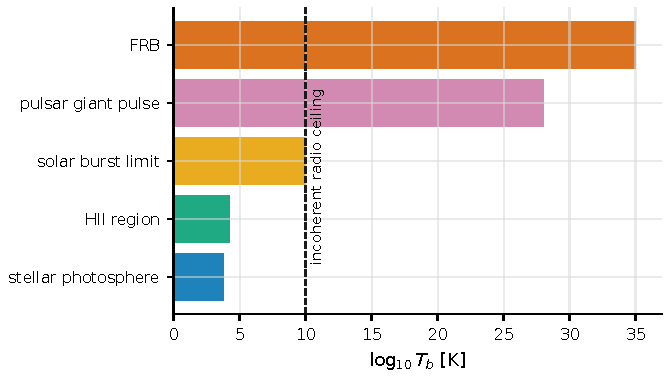
\includegraphics[width=0.82\linewidth]{figures/generated/chapter_09/ch09_brightness_temperature_scale.pdf}
\caption{亮温作为辐射机制的第一层判据。恒星光球和 HII 区落在普通热温度范围（对应占有数 \(\bar n_\nu\lesssim1\)）；太阳和恒星射电爆发若超过 \(10^{10}~{\rm K}\) 往往需要相干机制；脉冲星巨脉冲和 FRB 的亮温更高（占有数可达 \(10^{30}\) 以上），只能由相干发射或强束射几何解释。虚线标出常用的非相干射电上限量级。}
\label{fig:e16-brightness-temperature}
\end{figure}

亮温给我们的是一条硬的、经验性的门槛。Dulk 对太阳与恒星射电辐射的综述给出一条实用判据：非相干射电辐射的 \(T_b\) 很难超过 \(10^9\)--\(10^{10}~{\rm K}\)，这一上限主要来自回旋同步自吸收与能量学约束（占有数一旦太高，自吸收和辐射反作用就把它压回来；顺带一提，逆康普顿灾变 Kellermann--Pauliny-Toth 给出的是更高的 \(\sim10^{12}~{\rm K}\) 尺度，两者别混为一谈）；显著高于这个范围的爆发就必须请出相干机制，如等离子体辐射或 electron-cyclotron maser \citep{1985ARA&A..23..169D}。于是亮温标尺（图 \ref{fig:e16-brightness-temperature}）就成了机制判断的第一刀：占有数是 \(\lesssim1\) 的"稀薄热光"，还是 \(10^{20}\)、\(10^{30}\) 的"相干爆发"。但这只是第一刀——它只管平均能量密度合不合理，管不了这些光子是独立叠加还是协同发射。要分这一步，得动用光子统计。

\section{热辐射为什么天生是混沌光}
\label{sec:e16-thermal}

先看谱系里最"老实"的一档：热辐射。恒星光球、尘埃、HII 区、宇宙微波背景，都近似处在局部热平衡（local thermodynamic equilibrium）。它们的模式占有数由 Planck 分布给出，
\begin{equation}
  \bar n_\nu=\frac{1}{\exp(h\nu/k_BT)-1},
  \label{eq:e16-planck-occupation}
\end{equation}
\begin{formulaexplain}
\(\bar n_\nu\) 频率 \(\nu\) 模式的平均占有数；\(h\nu\) 单光子能量，\(T\) 物质温度。R--J 区（\(h\nu\ll k_BT\)）\(\bar n_\nu\approx k_BT/h\nu\gg1\)；Wien 区（\(h\nu\gg k_BT\)）\(\bar n_\nu\approx e^{-h\nu/k_BT}\ll1\)。
\end{formulaexplain}
这里 \(T\) 是物质的热温度。注意恒星光球的可见光常处在 Wien 区（\(h\nu/k_BT>1\)），所以颜色温度、有效温度、亮温三者不能混用——同一颗星，射电端 \(\bar n_\nu\) 大、光学端 \(\bar n_\nu\) 小。但无论落在哪个区，热态的\emph{统计性质}都一样，而这正是我们关心的。

为什么热辐射天生给混沌光（chaotic light）？物理图像是这样的：热光源里有海量独立的发射体（原子、离子、电子），每一个都在随机的时刻、以随机的相位发出一个小波列。探测器接到的总电场，是这千千万万个相位随机、幅度随机的小箭头的矢量和。这时候中心极限定理（central limit theorem）登场——大量独立随机量之和趋向高斯分布——所以窄带内的复电场 \(\hat E^{(+)}(t)\) 是一个\emph{复高斯随机过程}（complex Gaussian random process）。这不是巧合，是"许多独立事件相加"的必然结果。

高斯随机过程有一个漂亮的代数性质（第 \ref{chap:e08} 章证过，这里点名为已知结果）：它的四阶矩可以拆成二阶矩的乘积（矩定理 / Gaussian moment theorem）。把这条性质用到 \eqref{eq:e16-g2} 的分子上，就得到 Siegert（西格特）关系
\begin{equation}
  g^{(2)}(\tau)=1+\frac{|g^{(1)}(\tau)|^2}{M_{\rm eff}},
  \label{eq:e16-siegert}
\end{equation}
\begin{formulaexplain}
Siegert 关系：混沌（高斯）光的二阶相干完全由一阶相干决定。\(M_{\rm eff}\) 是被同时平均的模式数。单模（\(M_{\rm eff}=1\)、\(\tau=0\)）给出 \(g^{(2)}(0)=1+1=2\)，就是热光聚束峰。
\end{formulaexplain}
在单一时空--偏振模式里（\(M_{\rm eff}=1\)）取 \(\tau=0\)，因为 \(|g^{(1)}(0)|=1\)，立刻得到 \(g^{(2)}(0)=1+1=2\)。这就是热光聚束的种子，也是本章反复要用的锚点：\emph{只要是"许多独立发射体相加"，光场就是高斯混沌场，就自带 \(g^{(2)}(0)=2\) 的聚束峰。}热光并不神秘，它的聚束纯粹是相位随机叠加时"强度会成团涨落"的统计后果。

这个逻辑的力量在于它\emph{不挑机制}。只要满足"许多独立事件相加、窄带内相位随机"，谱形是什么无所谓，结论都是高斯混沌光。第一个例子是\emph{自由自由辐射}（bremsstrahlung，轫致辐射）：它不是黑体谱本身，而是无数电子在离子库仑场中被加速、各自发一次刹车辐射的连续谱。单次碰撞的相位完全不可预测，窄带内的复电场照样趋向高斯过程。稀薄电离气体中，发射系数的量级为
\begin{equation}
  j_\nu^{\rm ff}\propto
  n_e\,n_i\,T_e^{-1/2}
  \exp\!\left(-\frac{h\nu}{k_BT_e}\right)
  g_{\rm ff}(\nu,T_e),
  \label{eq:e16-free-free}
\end{equation}
\begin{formulaexplain}
\(j_\nu^{\rm ff}\) 自由自由发射系数；\(n_e,n_i\) 电子、离子数密度（\({\rm cm^{-3}}\)），\(T_e\) 电子温度，\(g_{\rm ff}\) Gaunt 因子（\(\sim1\) 到数十）。它是许多独立库仑碰撞贡献的连续谱。
\end{formulaexplain}
其中 \(n_e,n_i\) 是电子和离子数密度（\({\rm cm^{-3}}\)），\(T_e\) 是电子温度，\(g_{\rm ff}\) 是 Gaunt 因子。HII 区的 \(T_e\sim10^4~{\rm K}\)，星风、吸积流可以更高。谱形（射电端近平坦、高频指数衰减）和黑体完全不同，但光子统计一样是混沌热光，同样自带 \(g^{(2)}(0)=2\) 的种子。

不过谱要观测到，还得穿过介质，这就要放进辐射转移方程（radiative transfer equation）：
\begin{equation}
  \frac{{\rm d}I_\nu}{{\rm d}s}=j_\nu-\alpha_\nu I_\nu,
  \qquad
  S_\nu=\frac{j_\nu}{\alpha_\nu}.
  \label{eq:e16-radiative-transfer}
\end{equation}
\begin{formulaexplain}
\({\rm d}I_\nu/{\rm d}s\) 沿视线的强度变化；\(j_\nu\) 加入辐射，\(\alpha_\nu I_\nu\) 吸收辐射，\(S_\nu=j_\nu/\alpha_\nu\) 源函数。它把发射机制和光深连起来。
\end{formulaexplain}
\(s\) 是沿视线距离，\(j_\nu\) 是发射系数，\(\alpha_\nu\) 是吸收系数，源函数 \(S_\nu=j_\nu/\alpha_\nu\)。定义光深 \({\rm d}\tau_\nu=\alpha_\nu\,{\rm d}s\)，把 \eqref{eq:e16-radiative-transfer} 对一块均匀 slab 积分（这是一阶线性常微分方程，用积分因子 \(e^{\tau_\nu}\) 直接解，标准结果），再换成亮温，得到
\begin{equation}
  T_b=T_{\rm eff}\left(1-e^{-\tau_\nu}\right)+T_{\rm bg}\,e^{-\tau_\nu}.
  \label{eq:e16-tb-transfer}
\end{equation}
\begin{formulaexplain}
\(T_b\) 出射亮温；\(T_{\rm eff}\) 源函数对应温度，\(T_{\rm bg}\) 背景亮温，\(\tau_\nu\) 光深。薄源（\(\tau_\nu\ll1\)）只加一点点，厚源（\(\tau_\nu\gg1\)）趋向自身源函数。
\end{formulaexplain}
光深很小时 \(T_b\simeq T_{\rm eff}\tau_\nu+T_{\rm bg}\)（薄源只贡献小增量），光深很大时 \(T_b\to T_{\rm eff}\)（厚源热化到自身源函数）。这条式子常用来判断一个源是热化的、半透明的、还是非热占优的 \citep{1979rpa..book.....R,2011piim.book.....D,1985ARA&A..23..169D}。它也解释了亮温上限从何而来：一旦光深足够大，\(T_b\) 就被源函数（对热源就是物质温度）卡死，涨不上去。

小结这一节的物理：热辐射与自由自由辐射的共同点，不在谱形，而在"许多独立发射体相加"这条统计根。这条根让它们的电场都是高斯混沌场，都默认坐在 \(g^{(2)}(0)=2\) 那一档。这就是我们的"零点"——接下来所有其他机制，都要看它们是留在这一档、还是偏离。

\section{非热粒子：谱和偏振变了，统计却常常没变}
\label{sec:e16-nonthermal}

初学者最容易犯的一个错，是把"非热"（non-thermal）和"非高斯统计"划等号。这一节要专门破除它。同步辐射、逆康普顿——它们的\emph{谱和偏振}确实彻底偏离黑体，但它们的\emph{光子统计}多半仍然是高斯混沌光。原因还是那条根：只要发光的是许多独立粒子、窄带内相位随机，中心极限定理照样把电场压成高斯过程。

同步辐射（synchrotron radiation）来自相对论电子在磁场中的螺旋运动。单个电子的特征频率是
\begin{equation}
  \nu_c=\frac{3eB\sin\alpha}{4\pi m_ec}\,\gamma^2 ,
  \label{eq:e16-synch-critical}
\end{equation}
\begin{formulaexplain}
\(\nu_c\) 同步特征频率；\(e\) 元电荷，\(B\) 磁场，\(\alpha\) 投掷角（pitch angle），\(m_e\) 电子质量，\(\gamma\) Lorentz 因子。频率随 \(B\) 和 \(\gamma^2\) 增长，所以高能电子能把辐射推到很高频段。
\end{formulaexplain}
其中 \(e\) 是元电荷，\(B\) 磁场强度，\(\alpha\) 投掷角，\(m_e\) 电子质量，\(\gamma\) Lorentz 因子。提醒一句：这里的裸符号 \(\alpha\) 专指投掷角（pitch angle，电子速度与磁场的夹角），请勿与上一节的吸收系数 \(\alpha_\nu\)、下文将出现的同步谱指数 \(\alpha_{\rm syn}\) 混淆——三者靠语境和下标区分。代数字：\(B=1~{\rm G}\)、\(\gamma=10^3\)、\(\sin\alpha=1\)，得 \(\nu_c\simeq4.2\times10^{12}~{\rm Hz}\)（远红外）；换到星系际或喷流尺度的弱磁场 \(B=10^{-5}~{\rm G}\)，同一批电子主要辐射在射电。真实源的发射系数是所有能量电子的贡献叠加，
\begin{equation}
  j_\nu^{\rm syn}=\int P_\nu(E,B,\alpha)\,N(E)\,{\rm d}E ,
  \label{eq:e16-synch-emissivity}
\end{equation}
\begin{formulaexplain}
\(j_\nu^{\rm syn}\) 同步发射系数；\(P_\nu\) 单电子功率谱，\(N(E)\) 电子能量分布。积分说明观测谱是所有能量电子贡献之和——正是"许多独立发射体相加"。
\end{formulaexplain}
若电子能谱是幂律 \(N(E)\propto E^{-p}\)，光薄同步辐射给出幂律谱 \(I_\nu\propto\nu^{-\alpha_{\rm syn}}\)，谱指数 \(\alpha_{\rm syn}=(p-1)/2\)。同步辐射的招牌是高线偏振——均匀磁场里最大线偏振度为
\begin{equation}
  \Pi_{\rm syn}=\frac{p+1}{p+7/3}.
  \label{eq:e16-synch-polarization}
\end{equation}
\begin{formulaexplain}
\(\Pi_{\rm syn}\) 光薄同步辐射最大线偏振度；\(p\) 电子能谱指数。它是均匀磁场加幂律电子分布下偏振的理论上限。
\end{formulaexplain}
例如 \(p=2.4\) 时 \(\Pi_{\rm syn}\simeq72\%\)。实际喷流、超新星遗迹、脉冲星风云的偏振往往低得多，因为磁场方向杂乱、法拉第旋转、束内平均、多发射区叠加都会抵消偏振。请注意关键的一点：式 \eqref{eq:e16-synch-emissivity} 的积分号本身就在说"许多独立电子相加"，所以\emph{尽管谱是幂律、偏振很高，电场依然近似高斯混沌场，\(g^{(2)}(0)\) 依然默认是 2}。同步辐射改写的是平均谱和偏振（由非热电子分布和磁场几何决定），没改写光子统计这一档 \citep{1965ARA&A...3..297G,1970RvMP...42..237B,1978bllo.conf..328B,2012ApJ...752..157Z}。

逆康普顿散射（inverse Compton scattering）把低能种子光子踢到高能。Thomson 极限下，散射后光子能量的量级是
\begin{equation}
  h\nu_{\rm IC}\sim\gamma^2\,h\nu_{\rm seed}.
  \label{eq:e16-ic-energy}
\end{equation}
\begin{formulaexplain}
\(h\nu_{\rm seed}\) 种子光子能量，\(h\nu_{\rm IC}\) 散射后能量，\(\gamma\) 电子 Lorentz 因子。Thomson 极限中一次散射把光子能量提升约 \(\gamma^2\) 倍。
\end{formulaexplain}
热电子云中的多次散射，用 Compton \(y\) 参数衡量：
\begin{equation}
  y\simeq4\,\frac{k_BT_e}{m_ec^2}\,\max(\tau_T,\tau_T^2),
  \label{eq:e16-compton-y}
\end{equation}
\begin{formulaexplain}
\(y\) Comptonization 强度参数；前因子 \(4k_BT_e/m_ec^2\) 是单次散射的相对能量增益，\(\max(\tau_T,\tau_T^2)\) 估平均散射次数（\(\tau_T\) Thomson 光深）。它判断谱被电子云改写到什么程度。
\end{formulaexplain}
\(y\ll1\) 谱只被轻微改动；\(y\sim1\) 形成明显的 Comptonized 连续谱；\(y\gg1\) 趋向饱和 Comptonization。在 X 射线双星、AGN 冕（corona）、GRB 光球模型里，平均谱常由同步、热光子、逆康普顿几个分量混出来，单看谱指数几乎无法唯一定机制 \citep{1980A&A....86..121S,1999MNRAS.309..496G,2013ApJ...765..103L}。而这些散射过程涉及的仍是海量独立光子--电子事件，输出光场的统计还是留在混沌热光那一档。

\begin{figure}[tbp]
\centering
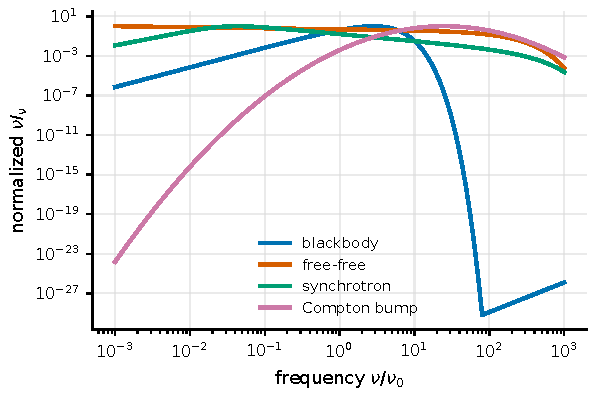
\includegraphics[width=0.84\linewidth]{figures/generated/chapter_09/ch09_spectral_mechanisms.pdf}
\caption{常见连续辐射机制的归一化谱形示意。黑体有热峰和 R--J 低频端；自由自由辐射在射电近平坦、高频指数衰减；同步辐射由非热电子能谱给出幂律加高低频截断；逆康普顿分量常表现为高能鼓包。四种谱形迥异，但只要是"许多独立粒子相加"，光子统计都默认落在 \(g^{(2)}(0)=2\) 的混沌热光那一档。}
\label{fig:e16-spectral-mechanisms}
\end{figure}

这一节的教学要点，一句话：\emph{谱和偏振能告诉你粒子分布和磁场几何，但告诉不了你光子统计。}热的、自由自由的、同步的、逆康普顿的——谱形从热峰到幂律到高能鼓包一路变化（图 \ref{fig:e16-spectral-mechanisms}），可它们共享同一条统计根，都是高斯混沌光。要让 \(g^{(2)}\) 真正偏离 2，必须打破"许多独立发射体相加"这个前提——这就把我们逼到下一节的相干机制。

\section{相干机制：突破亮温上限的少数出口}
\label{sec:e16-coherent}

要偏离混沌热光，只有一条路：让发射体不再独立，让大量电荷在相位上\emph{协同}起来。一旦协同，中心极限定理的前提就垮了，电场不再是高斯过程，占有数可以冲上 \(10^{20}\)、\(10^{30}\)，亮温突破那条 \(10^{10}~{\rm K}\) 的非相干上限。天体上做到这一点的机制屈指可数，本节逐个点名。

\paragraph{受激辐射类：maser 与激光}
\label{sec:e16-maser}

Maser（微波激射）从"负吸收"开始。若某条谱线上出现粒子数反转（population inversion，高能级比低能级还多），吸收系数就变成负的，\(\alpha_\nu<0\)。把它代进辐射转移，强度沿路径\emph{指数放大}：
\begin{equation}
  I_\nu(L)\simeq I_\nu(0)\,\exp(|\tau_m|),
  \qquad
  \tau_m=\int_0^L\alpha_\nu\,{\rm d}s<0 .
  \label{eq:e16-maser-gain}
\end{equation}
\begin{formulaexplain}
\(I_\nu(0),I_\nu(L)\) 路径前后强度；\(\tau_m<0\) 负吸收光深。未饱和时增益随 \(|\tau_m|\) 指数增长——这是高亮温窄线的来源。
\end{formulaexplain}
未饱和时增益对光深指数敏感，能把 \(T_b\) 推到极高；饱和后受激辐射耗尽反转，线宽、偏振、强度都由泵浦和几何接管。水 maser、OH maser、SiO maser 的亮温可以极高，占有数因而巨大。但要小心：天体 maser 的相干性通常由许多速度相干路径、湍动团块、偏振传播效应共同决定，\emph{不能}简单等同于实验室里那束单模激光的近相干态。Goldreich、Keeley、Kwan 与 Elitzur 的工作给出了源尺寸、饱和、线宽、偏振的基本约束 \citep{1972ApJ...174..517G,1973ApJ...179..111G,1974ApJ...190...27G,1982RvMP...54.1225E,1992ARA&A..30...75E}。受激辐射也不限于射电——Eta Carinae 的 Weigelt blobs 里，Fe II、O I 谱线在特定泵浦和光深下可出现激光或激光样放大，其线宽、位置、偏振和光子相关能检验反转与反馈几何 \citep{2004A&A...428..497J,2005NewA...10..361J,2008AIPC..984..216D}。只要泵浦、能级结构、逃逸路径合适，光学谱线也能带上非普通热光的统计特征。

电子回旋 maser（electron-cyclotron maser）是强磁化、低密度等离子体里的相干射电机制。它要求电子分布偏离平衡（如 loss-cone 分布），且回旋频率与等离子体频率的关系允许电磁波逃逸。回旋频率为
\begin{equation}
  \nu_B=\frac{eB}{2\pi m_ec}
       \simeq2.8~{\rm MHz}\left(\frac{B}{1~{\rm G}}\right).
  \label{eq:e16-cyclotron-frequency}
\end{equation}
\begin{formulaexplain}
\(\nu_B\) 电子回旋频率；\(e\) 电荷，\(B\) 磁场，\(m_e\) 电子质量。观测到的 maser 频率可反推发射区磁场量级。
\end{formulaexplain}
若在 GHz 频率看到基频或低次谐波的 electron-cyclotron maser，磁场量级就是几百 G 到几 kG。太阳、行星、褐矮星、低质量恒星的高圆偏振射电爆发都可落进这个框架 \citep{1982ApJ...259..844M,2006A&ARv..13..229T,2008ApJ...684..644H,1985ARA&A..23..169D}。

\paragraph{天线类：相干曲率辐射}
\label{sec:e16-curvature}

曲率辐射（curvature radiation）展示了通往相干性的另一条路——它不靠能级反转，而是让许多电荷在相位上协同运动，像一根天线。相对论电荷沿弯曲磁力线运动时，单个电荷的特征频率和功率为
\begin{equation}
  \nu_{\rm curv}=\frac{3c}{4\pi\rho}\gamma^3,
  \qquad
  P_{\rm curv}=\frac{2e^2c}{3\rho^2}\gamma^4 ,
  \label{eq:e16-curvature}
\end{equation}
\begin{formulaexplain}
\(\nu_{\rm curv}\) 曲率辐射特征频率，\(P_{\rm curv}\) 单粒子功率；\(\rho\) 磁力线曲率半径，\(\gamma\) Lorentz 因子。相干曲率辐射还需许多电荷相位同步。
\end{formulaexplain}
其中 \(\rho\) 是磁力线曲率半径。代数字：\(\rho=10^7~{\rm cm}\)、\(\gamma=300\)，先算前因子 \(3c/(4\pi\rho)\simeq7.2\times10^2~{\rm Hz}\)，再乘 \(\gamma^3=2.7\times10^7\)，得 \(\nu_{\rm curv}\sim2\times10^{10}~{\rm Hz}\)（仍属射电／微波波段）。单个粒子的曲率辐射太弱；相干曲率辐射要求许多电荷在小于波长的纵向尺度上成团（bunching），电场振幅\emph{相加}而非功率相加，于是总功率近似随粒子数\emph{平方}增长。这就是"天线"的精髓：\(N\) 个电荷若相位同步，辐射功率 \(\propto N^2\) 而非 \(N\)。这个思路长期用于脉冲星相干射电，也被搬进 FRB 模型 \citep{1977ApJ...212..800C,2018MNRAS.477.2470L}。

FRB 把相干机制推到极端。Lorimer burst 给出了毫秒时标、冷等离子体色散、\(T_b\sim10^{34}~{\rm K}\) 的第一组证据；重复源和 CHIME 样本显示重复、偏振、频率漂移、微结构、宿主环境都进模型；SGR 1935+2154 的 2020 年事件把银河系 magnetar 和 FRB 样射电暴直接连上了 \citep{2007Sci...318..777L,2019A&ARv..27....4P,2022A&ARv..30....2P,2020Natur.587...54C,2020Natur.587...59B}。众多模型大致两类：靠粒子数反转或激波的 maser 类，和靠电荷团块或电流片的天线/曲率类。微秒以下结构、强偏振、频率漂移、多波段非探测共同约束发射半径、Lorentz 因子、等离子体密度和辐射效率。

这一节的物理落点：相干机制之所以能突破亮温上限、把占有数推到天文数字，是因为它们打破了"独立发射体相加"这个前提，让电荷协同起来。它们的光子统计\emph{原则上}可以偏离混沌热光——但请记住，这里说的偏离，指的是极高占有数下受激/协同发射的特征，并不等于我们在实验室里追求的那种压缩态、反聚束的非经典光。真正的非经典光需要 \(g^{(2)}(0)<1\)，而天体上，哪怕源本身偏离了热统计，我们能不能\emph{测到}这份偏离，还要过下一节这一关。

\section{为什么天体上极难隔离真正的非经典光}
\label{sec:e16-dilution}

现在到了本章最要紧、也最容易被浪漫化的一点。前面说单模热光 \(g^{(2)}(0)=2\)，相干机制可能偏离——听上去只要架好探测器就能读出机制指纹。真实观测却几乎总是把这些指纹\emph{抹平}。抹平它的，是"模式稀释"（mode dilution）。

物理图像：\(g^{(2)}(0)=2\) 的那个漂亮聚束峰，只在\emph{单一}时空--偏振模式里成立。可真实望远镜同时收进一大堆模式——望远镜的接收面覆盖许多空间相干斑（空间模式 \(M_{\rm sp}\)），它对两个偏振都敏感（偏振模式 \(M_{\rm pol}\)），它的时间分辨率 \(\Delta t\) 又远宽于相干时间 \(\tau_c\)（时间模式 \(\sim\Delta t/\tau_c\)）。这些模式的涨落彼此独立，一平均，聚束峰就被摊薄。把 Siegert 关系 \eqref{eq:e16-siegert} 里的 \(M_{\rm eff}\) 写细，
\begin{equation}
  g^{(2)}_{\rm meas}(0)-1\simeq\frac{1}{M_{\rm eff}},
  \qquad
  M_{\rm eff}\simeq M_{\rm sp}\,M_{\rm pol}\left(1+\frac{\Delta t}{\tau_c}\right).
  \label{eq:e16-mode-dilution}
\end{equation}
\begin{formulaexplain}
\(M_{\rm eff}\) 有效混合模式数；\(M_{\rm sp},M_{\rm pol}\) 空间、偏振模式数，\(\Delta t/\tau_c\) 时间 bin 对相干时间的平均。模式越多，能测到的聚束对比度 \(g^{(2)}_{\rm meas}(0)-1\) 越低。
\end{formulaexplain}
其中 \(M_{\rm sp}\) 是被混合的空间模式数，\(M_{\rm pol}\) 是偏振模式数，\(\Delta t\) 是电子学或软件时间 bin，\(\tau_c\simeq1/\Delta\nu\) 是由光谱带宽决定的相干时间。代真实数字：可见光 \(\lambda=500~{\rm nm}\)、谱带宽 \(\Delta\lambda\simeq1~{\rm nm}\)（这里的 nm 是波长单位，标的是 \(\Delta\lambda\) 而非频率带宽），用 \(\Delta\nu\simeq c\,\Delta\lambda/\lambda^2\approx1.2\times10^{12}~{\rm Hz}\) 换成频率带宽，对应的相干时间约 \(\tau_c\simeq1/\Delta\nu\sim0.8~{\rm ps}\)；而典型电子学时间分辨率 \(\Delta t\sim100~{\rm ps}\)，于是 \(\Delta t/\tau_c\sim125\)。哪怕只有一个空间、一个偏振模式，单模热光本该到 2 的聚束峰，被压到 \(g^{(2)}_{\rm meas}(0)-1\sim1/125\lesssim0.01\)——足足两个数量级（图 \ref{fig:e16-mode-dilution}）。这就是为什么 Hanbury Brown--Twiss 强度干涉在星际尺度上信号那么微弱，为什么每一分对比度都要用窄带滤波、偏振选择、空间模式控制去"抢"，而每一步抢救对比度都以牺牲光子率为代价（第 \ref{chap:e10} 章会把这笔账算清）。

\begin{figure}[tbp]
\centering
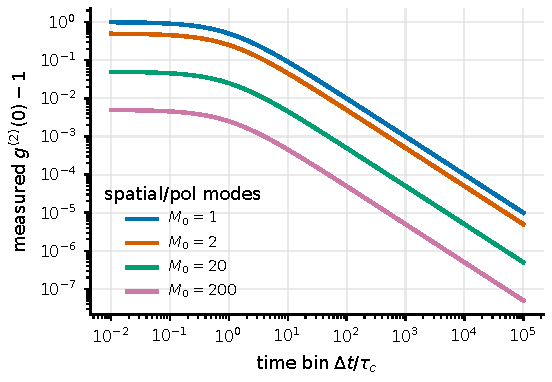
\includegraphics[width=0.82\linewidth]{figures/generated/chapter_09/ch09_thermal_mode_dilution.pdf}
\caption{热光聚束对比度随有效模式数下降。横轴是时间 bin 与相干时间之比，曲线上的 \(M_0\) 代表进入同一个相关估计器的空间与偏振模式数。即便源本身是纯热光，宽时间 bin、多偏振混合、多空间模式混合都会把 \(g^{(2)}(0)-1\) 拉向零——这正是天体上极难看到光子统计指纹的根本原因。}
\label{fig:e16-mode-dilution}
\end{figure}

现在把这层稀释叠到前面的图景上，就明白"天体上为什么极难隔离真正的非经典光"了。第一，多数机制\emph{本来}就给混沌热光（\(g^{(2)}(0)=2\)），非经典（\(g^{(2)}(0)<1\)）的候选屈指可数。第二，即便某个相干机制原则上偏离了热统计，模式稀释也会把可测的偏离压到 \(10^{-2}\) 甚至更低。第三，就算你信号还在，仪器和传播效应会伪造出假的相关：死时间、afterpulsing、时间戳量化、触发选择会改写到达时间相关（假的 \(g^{(2)}\) 结构）；等离子体闪烁、散射尾、引力微透镜、频率依赖吸收会造出跨频相关；热背景叠一条窄 maser 线、或同步连续谱叠一个相干脉冲，会让平均谱看着平滑、光子统计却不再单一。所以任何一个"反常的 \(g^{(2)}\) 峰"，都必须先和仪器、传播、混合源逐项对账，才敢往"非经典"上想（图 \ref{fig:e16-g2-diagnostics} 把单模热光、多模稀释、相干态、窄相干线四种情形的 \(g^{(2)}(\tau)\) 形状放在一起对照，正是这一步逐项排查的参照图）。第 \ref{chap:e13} 章和第 \ref{chap:e14} 章的事件表、时间移位背景、协方差估计，提供的正是这种逐项排查所需的分析层。

\begin{figure}[tbp]
\centering
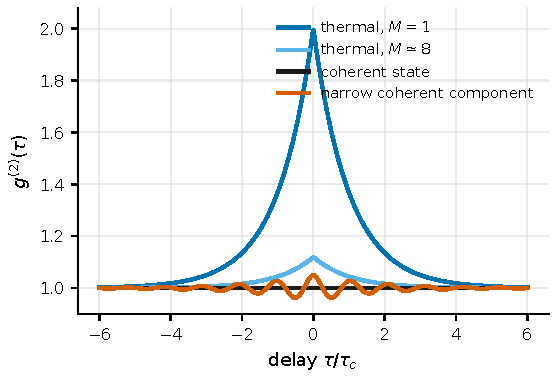
\includegraphics[width=0.82\linewidth]{figures/generated/chapter_09/ch09_radiation_g2_diagnostics.pdf}
\caption{不同光场的 \(g^{(2)}(\tau)\)。单模热光在零延迟给出高度为 2 的聚束峰；多模平均把峰值压低（式 \eqref{eq:e16-mode-dilution}）；理想相干态接近 1；窄相干谱线或受激成分可以在接近泊松的背景上留下小幅振荡或窄峰。横轴按相干时间 \(\tau_c\) 归一化。}
\label{fig:e16-g2-diagnostics}
\end{figure}

于是机制判断的正确姿势，是把所有能测的量收进同一个观测向量里联合诊断，而不是死盯平均谱：
\begin{equation}
  \bm{d}=
  \left\{
  I_\nu(t),\,
  Q_\nu(t),U_\nu(t),V_\nu(t),\,
  g^{(2)}_{ab}(\tau;\nu_i,\nu_j),\,
  \Delta t_{\rm var},\,
  \Omega_{\rm s}
  \right\}.
  \label{eq:e16-diagnostic-vector}
\end{equation}
\begin{formulaexplain}
\(\bm{d}\) 机制诊断观测向量；同时收集强度、Stokes 偏振、二阶相关、变异时标、角尺度。机制判断要靠这些量\emph{联合}约束，单看平均谱不够。
\end{formulaexplain}
其中 \(Q,U,V\) 是 Stokes 参数，下标 \(a,b\) 标记望远镜、偏振或频率通道，\(\Delta t_{\rm var}\) 是变异时标，\(\Omega_{\rm s}\) 是角尺度约束。把各机制放到这个向量里，指纹就分开了：热源——低偏振、有限 \(T_b\)、（稀释后残余的）热聚束；光薄同步——高线偏振、幂律谱；maser——窄线、极高 \(T_b\)、强偏振；FRB——极高 \(T_b\)、毫秒到微秒结构、色散、强偏振。而散射和等离子体传播会改变时间结构和频谱，却\emph{不该}被误当成源本身的发射统计。图 \ref{fig:e16-diagnostic-plane} 把其中两条轴（亮温、偏振分数，点大小示意可测二阶相干对比度）画成一张诊断平面，帮我们一眼定位一个源大致落在哪一类机制里。

\begin{figure}[tbp]
\centering
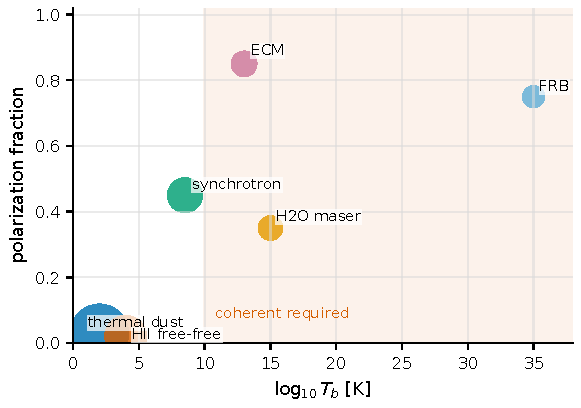
\includegraphics[width=0.86\linewidth]{figures/generated/chapter_09/ch09_diagnostic_plane.pdf}
\caption{辐射机制的联合诊断平面。横轴亮温，纵轴偏振分数，点大小表示可测二阶相干对比度的量级。热尘埃和 HII 区在低亮温低偏振区；同步辐射偏振较高但亮温通常低于相干爆发；electron-cyclotron maser、分子 maser 和 FRB 进入高亮温区，需要相干发射、泵浦或电荷成团来解释。}
\label{fig:e16-diagnostic-plane}
\end{figure}

\section{本章要点}
\label{sec:e16-summary}

\begin{itemize}
  \item \textbf{一句话主线。}把辐射机制翻译成"占有数 + 光子统计"：平均谱 \(I_\nu\) 只是一阶信息，光子到达相关（\(g^{(2)}\)）、偏振相关、跨频联合概率才是机制的指纹。
  \item \textbf{亮温就是占有数。}在 Rayleigh--Jeans 定义下 \(\bar n_\nu=k_BT_b/(h\nu)\) 精确成立（式 \eqref{eq:e16-occupation-from-tb}）。恒星可见光 \(\bar n_\nu\sim10^{-2}\)（稀薄），FRB \(\bar n_\nu\sim10^{36}\)（协同）。非相干射电亮温上限约 \(10^{9}\)--\(10^{10}~{\rm K}\)，超过就需相干机制。
  \item \textbf{热与非热都默认给混沌光。}只要"许多独立发射体相加、窄带内相位随机"，电场就是高斯过程，Siegert 关系给单模 \(g^{(2)}(0)=2\)（式 \eqref{eq:e16-siegert}）。黑体、自由自由、同步、逆康普顿——谱和偏振各异，光子统计同属混沌热光那一档。
  \item \textbf{只有相干机制可能偏离。}maser／激光靠粒子数反转和受激辐射，相干曲率辐射靠电荷成团（功率 \(\propto N^2\)）。它们打破"独立相加"前提，占有数和亮温冲破上限——但天体 maser 不等于实验室单模激光。
  \item \textbf{非经典光极难隔离。}模式稀释（式 \eqref{eq:e16-mode-dilution}）把 \(g^{(2)}_{\rm meas}(0)-1\sim1/M_{\rm eff}\) 压到 \(10^{-2}\) 甚至更低；候选机制本就稀少；仪器与传播效应还会伪造相关。机制判断必须用联合诊断向量 \eqref{eq:e16-diagnostic-vector}，并借第 \ref{chap:e13}、\ref{chap:e14} 章的排查工具对账。
\end{itemize}

\noindent\textbf{想一想。}(1) 一颗恒星的射电端和光学端，物质温度相同，为什么占有数 \(\bar n_\nu\) 差好几个量级？(2) 同步辐射谱是幂律、偏振可达 70\%，凭什么说它的光子统计和黑体属同一档？(3) 若你在数据里看到 \(g^{(2)}(0)=1.01\)，在下"探到聚束"的结论前，你至少要排除哪三类假信号？

\chapter{恒星作为量子光源}
\label{chap:e17}

\begin{chapteropening}
上一章我们把各种天体辐射机制翻译成了量子语言：黑体、热光、受激辐射各自对应怎样的光子统计。现在把这套语言对准夜空里最普通、也最可靠的一类源——恒星。它们的光球（photosphere）近似一块发着热光的表面，角直径落在毫角秒（milliarcsecond, mas）量级，亮星每秒送来的光子多到足以做相关测量。更妙的是，强度干涉（intensity interferometry）只测两台望远镜光强涨落的相关，直接读出 \(|V|^2\)，完全不要求它们之间保持光学相位。这一章要回答一个问题：当我们把恒星不再当成一个点，而当成一块有结构的发光表面时，边缘昏暗、快速自转、星盘、双星、脉动，这些物理各自会在 \(|V(B)|^2\) 曲线上刻下怎样一道可分辨的指纹？我们会一路回收第 \ref{chap:e10} 章的 van Cittert--Zernike 定理与均匀圆盘，和第 \ref{chap:e11} 章的角直径、多基线成像，把它们落到 VERITAS 对 \(\beta\) UMa、\(\gamma\) Cas 等真实恒星的观测上 \citep{1956Natur.177...27B,1974MNRAS.167..121H,1974iiia.book.....H,2020NatAs...4.1164A,2024MNRAS.529.4387A}。
\end{chapteropening}

\section{为什么恒星是最稳的标定场}
\label{sec:e17-why-stars}

先说一个直觉：要检验一把尺子准不准，你会拿一个"你大致知道尺寸、而且不会乱动"的东西去量它。恒星恰好就是量子天文学这把新尺子的理想标定物。光球在局部热平衡（local thermodynamic equilibrium, LTE）下发出近似黑体的连续谱，谱形和总流量都能用成熟的恒星大气模型描述；亮星足够亮，光子统计误差可以靠积分时间压下去；而它们的角直径正好落在可见光百米基线能分辨的窗口。第 \ref{chap:e16} 章已经讲过，这种热光在单个相干模式里满足 \(g^{(2)}(0)=2\)——光子成群到来，涨落是相干态的两倍。

但真实望远镜看到的 \(g^{(2)}(0)-1\) 远小于 1。原因是模式稀释（mode dilution）：一次测量里混进了大量空间、偏振、频率和时间模式，每个模式各自贡献一份独立的热涨落，平均下来对比度被压低。第 \ref{chap:e08} 章给出的定量表述是 Siegert 关系里的那个稀释因子 \(\zeta\)，它约等于"单个相干模式占据的时空体积除以探测器实际接收的时空体积"。放到恒星上，这不是抽象命题：Vega 的 photon-counting 强度干涉实验在零基线测得 \(\langle g^{(2)}\rangle=1.0034\pm0.0008\)，只比 1 高出千分之三；在约 \(2~{\rm km}\) 基线上则测不到显著相关，这与 Vega 约 \(3.3~{\rm mas}\) 的角直径完全相容——星太大，公里基线早已把它分辨掉，可见度落到接近零 \citep{2021MNRAS.506.1585Z}。这就是第 \ref{chap:e08} 章模式稀释在一颗真实恒星身上的样子。

\paragraph{强度相关直接给出平方可见度}
\label{sec:e17-g2-vis}

强度干涉测的是两台望远镜光强涨落的零延迟相关。对热光，扣除背景、做完时间移位归一化之后，这个相关的超额部分正比于天空亮度分布的一个傅里叶模的模平方：
\begin{equation}
  g^{(2)}_{ij}(0)-1 \;=\; |\gamma_{ij}|^2 \;\simeq\; \bigl|V(u_{ij},v_{ij})\bigr|^2 .
  \label{eq:e17-g2-vis}
\end{equation}
\begin{formulaexplain}
\(g^{(2)}_{ij}(0)\)：望远镜 \(i,j\) 的零延迟强度相关。\(\gamma_{ij}\)：两台望远镜间的复相干度。\(V\)：归一化复可见度，\((u,v)\) 是投影基线除以波长。这条式子说：热光的强度相关超额，就是天空亮度傅里叶模的模平方。
\end{formulaexplain}
逐个交代符号。\(g^{(2)}_{ij}(0)\) 无量纲，是把两路光电流（或光子计数）在同一时刻相乘、再对各自平均归一化的结果，第 \ref{chap:e08} 章已推导过它对热光取 2、对相干态取 1。\(\gamma_{ij}\) 是复相干度，模在 0 到 1 之间；\((u,v)=\bm{B}_\perp/\lambda\) 是把投影基线 \(\bm{B}_\perp\)（单位 cm）除以波长 \(\lambda\)（单位 cm）得到的空间频率，量纲是"每弧度多少个波长"，也就是每弧度的条纹数。式 \eqref{eq:e17-g2-vis} 的左边来自真实数据处理——延迟直方图、时间移位背景扣除、归一化相关；右边则是纯几何的天空亮度傅里叶变换。关键在于：右边取了模平方，复相位彻底丢失。这意味着 \(|V|^2\) 对天空图像的整体平移和镜像翻转都不敏感（平移只改变傅里叶相位、镜像取共轭，模平方都看不出来）。但只要目标结构本身有确定的几何——一个圆盘的直径、一个椭圆的轴比、一对双星的间距——这些量仍然能从 \(|V|^2\) 精确读出。这正是本章后面每一节要做的事。

\paragraph{基线长度与角尺度是同一把标尺}
\label{sec:e17-baseline}

要分辨一个角尺度为 \(\theta\) 的结构，需要多长的基线？答案来自 van Cittert--Zernike 定理里最朴素的量纲关系：
\begin{equation}
  B \;\sim\; \frac{\lambda}{\theta}
  \;\simeq\; 103~{\rm m}
  \left(\frac{\lambda}{500~{\rm nm}}\right)
  \left(\frac{\theta}{1~{\rm mas}}\right)^{-1}.
  \label{eq:e17-baseline}
\end{equation}
\begin{formulaexplain}
\(B\)：所需基线长度。\(\lambda\)：观测波长。\(\theta\)：目标角尺度。可见光下，毫角秒的恒星对应百米基线，公里基线才够得着毫角秒以下的表面细节。
\end{formulaexplain}
把这个数量级算给自己看，才算真懂。取 \(\lambda=500~{\rm nm}=5\times10^{-7}~{\rm m}\)，\(\theta=1~{\rm mas}\)。1 mas 换成弧度要乘 \(4.848\times10^{-9}\)（因为 \(1~{\rm arcsec}=1/206265~{\rm rad}\)，再除以 1000），即 \(\theta=4.848\times10^{-9}~{\rm rad}\)。于是
\[
  B\sim\frac{\lambda}{\theta}=\frac{5\times10^{-7}~{\rm m}}{4.848\times10^{-9}}
  \approx 103~{\rm m}.
\]
这就是式 \eqref{eq:e17-baseline} 里那个系数 103 m 的来历。它告诉我们：一颗 \(1~{\rm mas}\) 的恒星，在可见光里要用百米基线才开始明显被分辨；而 \(0.1~{\rm mas}\) 的表面结构（比如自转扁率、星斑）需要公里量级的基线。历史上 Narrabri 强度干涉仪用 \(10\)--\(188~{\rm m}\) 的可变基线和两面 \(6.7~{\rm m}\) 反射面，测出了 32 颗亮星的角直径 \citep{1974MNRAS.167..121H,1974iiia.book.....H}。今天的 VERITAS、MAGIC 以及未来的 CTA 类阵列，用 \(>10~{\rm m}\) 口径的切伦科夫（Cherenkov）望远镜、更大的收光面积和数字相关器，重新打开了这个参数空间 \citep{2020NatAs...4.1164A,2024MNRAS.529.4387A}。

信噪比的标度已经在第 \ref{chap:e11} 章的式 \eqref{eq:e11-snr} 里给全了，这里只点名它对恒星选样的直接含义：光子率越高、电子带宽越大、积分越久，\(|V|^2\) 的误差越小（信噪比随积分时间只按平方根涨）；而背景光、探测器死时间、有限的时间分辨率和系统协方差决定了这种统计增益到哪里就"赚不动"了。所以第一批目标自然偏向亮、热、蓝、且角直径在百米基线上就能分辨的恒星 \citep{2013MNRAS.430.3187R,2020NatAs...4.1164A}。这句话不是口号，它是下一节"怎样布基线"的物理依据。

\section{怎样从平方可见度读出角直径和温度}
\label{sec:e17-diameter-teff}

从数据到半径，第一步是把恒星暂时当成一枚"均匀发光的硬币"——只有一个参数：角直径 \(\theta\)。这就是第 \ref{chap:e10} 章的均匀圆盘（uniform disk）模型，其可见度由式 \eqref{eq:e10-disk} 给出，
\[
  V_{\rm UD}(B)=\frac{2J_1(x)}{x},\qquad x=\frac{\pi\theta B}{\lambda},
\]
其中 \(J_1\) 是一阶贝塞尔函数，\(x\) 是无量纲的"分辨程度"。这里 \(B\) 是投影基线，\(\lambda\) 是有效波长，\(\theta\) 要用弧度（若以 mas 给出，乘 \(4.848\times10^{-9}\)）。强度干涉拟合的是 \(|V_{\rm UD}|^2\)，复相位已经被模平方抹掉。曲线上信息最密的地方是第一零点附近（\(x=3.8317\)，对应 \(B_0\approx1.22\lambda/\theta\)）——那里 \(|V|^2\) 对角直径最敏感；但零点附近 \(|V|^2\) 太小，背景和系统误差会盖过信号。所以实测要覆盖短、中、长三段基线：短基线固定总通量和相关归一化，中等基线给出直径的下降斜率，长基线检验模型是否还需要边缘昏暗、扁率或伴星。

\begin{figure}[tbp]
\centering
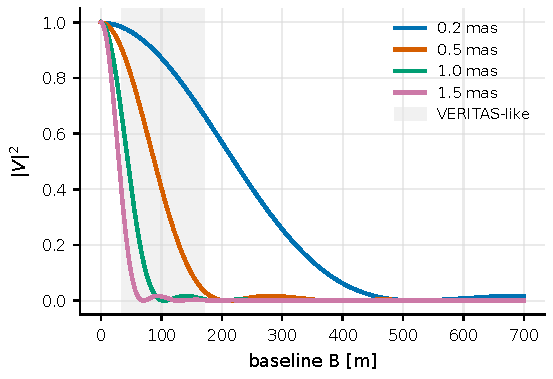
\includegraphics[width=0.82\linewidth]{figures/generated/chapter_10/ch10_stellar_diameter_visibility.pdf}
\caption{均匀圆盘恒星的 \(|V|^2\) 随基线变化。波长取 \(416~{\rm nm}\)，接近 VERITAS 强度干涉的观测波长。角直径越大，可见度下降得越快；灰色区域标出 \(35\)--\(170~{\rm m}\) 的 VERITAS 量级投影基线范围，适合测量约 \(0.5\)--\(1.5~{\rm mas}\) 的亮星。}
\label{fig:e17-diameter-visibility}
\end{figure}

\paragraph{角直径加总流量等于有效温度}
\label{sec:e17-teff}

量出角直径之后，只要再知道这颗星在地球处的总辐射流量，就能拿到它的有效温度（effective temperature）。推导只需要 Stefan--Boltzmann 定律加一步几何。恒星光度 \(L=4\pi R^2\sigma_{\rm SB}T_{\rm eff}^4\)，其中 \(R\) 是半径。传到距离 \(d\) 处，地球接收到的 bolometric flux 是 \(F_{\rm bol}=L/(4\pi d^2)=R^2\sigma_{\rm SB}T_{\rm eff}^4/d^2\)。而角直径与半径的关系是 \(\theta_{\rm LD}=2R/d\)，即 \(R/d=\theta_{\rm LD}/2\)，于是 \(R^2/d^2=\theta_{\rm LD}^2/4\)。代回去，距离 \(d\) 自动消掉：
\begin{equation}
  F_{\rm bol}=\frac{\theta_{\rm LD}^2}{4}\,\sigma_{\rm SB}T_{\rm eff}^4,
  \qquad
  T_{\rm eff}=\left(\frac{4F_{\rm bol}}{\sigma_{\rm SB}\theta_{\rm LD}^2}\right)^{1/4}.
  \label{eq:e17-teff}
\end{equation}
\begin{formulaexplain}
\(F_{\rm bol}\)：地球处测得的总辐射流量（\({\rm erg\,s^{-1}\,cm^{-2}}\)）。\(\theta_{\rm LD}\)：边缘昏暗角直径。\(\sigma_{\rm SB}\)：Stefan--Boltzmann 常数。角直径与总流量合起来，不需要知道距离就能定出有效温度。
\end{formulaexplain}
注意这个漂亮的地方：距离 \(d\) 在推导中被约掉了，所以 \(T_{\rm eff}\) 是一个"不依赖距离标尺"的量——你只需要测角直径和流量。\(\theta_{\rm LD}\) 下标 LD 提醒我们，这里该用边缘昏暗角直径（下一节解释为什么不能用均匀圆盘直径），单位是弧度或 mas；\(\sigma_{\rm SB}=5.67\times10^{-5}~{\rm erg\,s^{-1}\,cm^{-2}\,K^{-4}}\)（CGS）。

对同一颗星，我们更关心测量误差怎样传到 \(T_{\rm eff}\)。因为 \(T_{\rm eff}\propto F_{\rm bol}^{1/4}\theta_{\rm LD}^{-1/2}\)，取对数得 \(\ln T_{\rm eff}=\tfrac14\ln F_{\rm bol}-\tfrac12\ln\theta_{\rm LD}+{\rm const}\)。微分：\({\rm d}\ln T_{\rm eff}=\tfrac14\,{\rm d}\ln F_{\rm bol}-\tfrac12\,{\rm d}\ln\theta_{\rm LD}\)。若 \(F_{\rm bol}\) 与 \(\theta_{\rm LD}\) 的误差独立，方差按平方相加，系数取平方：
\begin{equation}
  \left(\frac{\sigma_T}{T_{\rm eff}}\right)^2
  \simeq
  \frac{1}{16}\left(\frac{\sigma_F}{F_{\rm bol}}\right)^2
  +\frac{1}{4}\left(\frac{\sigma_\theta}{\theta_{\rm LD}}\right)^2 .
  \label{eq:e17-teff-error}
\end{equation}
\begin{formulaexplain}
\(\sigma_T,\sigma_F,\sigma_\theta\)：温度、总流量、角直径的绝对误差。因为 \(T_{\rm eff}\propto F_{\rm bol}^{1/4}\theta_{\rm LD}^{-1/2}\)，同样的百分比误差下，角直径那一项（系数 \(1/4\)）比流量那一项（系数 \(1/16\)）权重大四倍。
\end{formulaexplain}
系数 \(1/16=(1/4)^2\) 和 \(1/4=(1/2)^2\) 正是指数的平方。结论是：角直径的相对误差进入 \(T_{\rm eff}\) 的权重是流量的四倍，因此往往是角直径主导了温度的精度。这正是强度干涉的价值所在——它把一个原本靠模型间接推断的角直径，变成了直接测量。VERITAS 对 \(\beta\) Ursae Majoris（\(\beta\) UMa）的强度干涉观测给出 \(\theta_{\rm LD}=1.07\pm0.04\,({\rm stat})\pm0.05\,({\rm sys})~{\rm mas}\)，代进式 \eqref{eq:e17-teff} 得到 \(T_{\rm eff}\simeq9700\pm200\pm200~{\rm K}\)，还能进一步约束 Ursa Major 移动星群的年龄 \citep{2024ApJ...966...28A}。而 VERITAS 首次现代强度干涉巡测测的 \(\beta\) Canis Majoris（\(\beta\) CMa）和 \(\epsilon\) Orionis（\(\epsilon\) Ori）两颗亮蓝星，正是这套方法在真实天空里的开场 \citep{2020NatAs...4.1164A}。

\begin{figure}[tbp]
\centering
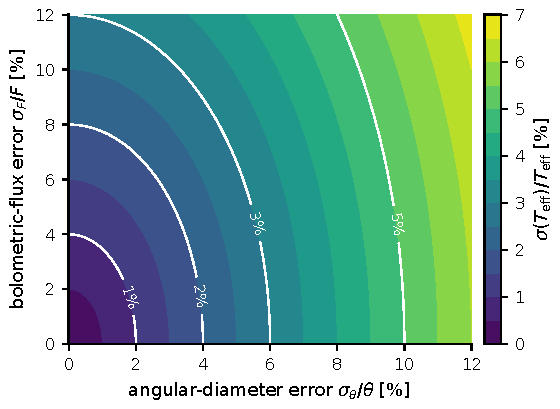
\includegraphics[width=0.78\linewidth]{figures/generated/chapter_10/ch10_teff_error_budget.pdf}
\caption{由 \(F_{\rm bol}\) 和 \(\theta_{\rm LD}\) 推导 \(T_{\rm eff}\) 的误差传播。横轴是角直径相对误差，纵轴是总流量相对误差，颜色给出有效温度相对误差。由于 \(T_{\rm eff}\propto F_{\rm bol}^{1/4}\theta_{\rm LD}^{-1/2}\)，角直径误差通常比同等百分比的流量误差更"值钱"。}
\label{fig:e17-teff-error}
\end{figure}

\paragraph{加上距离就得到半径和光度}
\label{sec:e17-radius}

如果这颗星的距离 \(d\) 由 Gaia 视差独立给出，那么角直径就能翻译成物理半径，Stefan--Boltzmann 定律再给出光度：
\begin{equation}
  R=\frac{1}{2}\theta_{\rm LD}\,d,\qquad
  L=4\pi R^2\sigma_{\rm SB}T_{\rm eff}^4 .
  \label{eq:e17-radius}
\end{equation}
\begin{formulaexplain}
\(R\)：恒星物理半径。\(d\)：距离。\(L\)：光度。角直径给出"天空上多大"，距离把它变成"实际多大"，再由 Stefan--Boltzmann 定律得到"发多亮"。
\end{formulaexplain}
第一式就是 \(\theta_{\rm LD}=2R/d\) 的改写；\(\theta_{\rm LD}\) 用弧度，\(d\) 与 \(R\) 同单位（比如都用 cm，或 \(d\) 用 pc、\(R\) 用 \(R_\odot\) 时记得换算）。把 Gaia 视差、强度干涉角直径和 \(F_{\rm bol}\) 三者联合，一颗恒星就落到赫罗（HR）图上一个带协方差的小区域里。这个小区域和恒星演化轨迹一比对，就约束了质量、年龄，以及混合长度、对流超射、自转等模型参数。红外流量法、Mark III 与 CHARA 等振幅干涉给出的角直径、以及强度干涉角直径，在这一层面是互相印证的独立标尺 \citep{1977MNRAS.180..177B,1991AJ....101.2207M,1994A&A...282..899B,2003AJ....126.2502M,2005ApJ...626..446R}。

\section{边缘昏暗为什么不是小修正}
\label{sec:e17-limb-darkening}

把恒星当均匀硬币，有一个必须还的债：真实恒星的圆面边缘更暗。原因很物理——当你看向圆盘中心时，视线垂直插进大气，看到的是较深、较热的层；当你看向边缘时，视线以很斜的角度掠过，只能看到较浅、较冷的高层。温度低，亮度就低，于是边缘发暗，这叫边缘昏暗（limb darkening）。最简单的线性模型是
\begin{equation}
  I(\mu)=I(1)\,[1-u_\lambda(1-\mu)],
  \qquad
  \mu=\sqrt{1-r^2}.
  \label{eq:e17-linear-ld}
\end{equation}
\begin{formulaexplain}
\(I(\mu)\)：不同视角处的表面亮度。\(\mu\)：表面法线与视线夹角的余弦。\(r\)：归一化投影半径（圆心 \(r=0\)，边缘 \(r=1\)）。\(u_\lambda\)：波长相关的边缘昏暗系数。它把"边缘变暗"压缩成一个参数。
\end{formulaexplain}
逐项看：\(r\) 是投影圆盘上的半径除以恒星半径，取值 0 到 1；圆心处视线垂直、\(\mu=1\)，边缘处视线掠射、\(\mu=0\)，几何关系正是 \(\mu=\sqrt{1-r^2}\)。\(I(1)\) 是圆心亮度。\(u_\lambda\) 是边缘昏暗系数，\(u_\lambda=0\) 退回均匀圆盘，\(u_\lambda\) 越大边缘越暗；它无量纲，且强烈依赖波长——热星在蓝光、冷巨星在分子吸收带、Mira 变星在不同脉动相位，\(u_\lambda\) 都不同。现代分析通常不用这条线性式，而是直接从大气模型生成合成的 \(I(\mu)\) 再算可见度；线性 \(u_\lambda\) 主要用来做数量级估算和直觉 \citep{1974MNRAS.167..475H,1992A&A...259..227D,1997A&A...327..199H,2015MNRAS.453.3821P}。

\paragraph{任意径向剖面的可见度是一次 Hankel 变换}
\label{sec:e17-hankel}

要知道边缘昏暗如何改可见度曲线，需要一个能吃"任意径向亮度剖面"的公式。对任何轴对称（圆对称）的亮度分布 \(I(r)\)，它的可见度就是径向的 Hankel 变换：
\begin{equation}
  V(x)=
  \frac{\displaystyle\int_0^1 I(r)\,J_0(xr)\,r\,{\rm d}r}
       {\displaystyle\int_0^1 I(r)\,r\,{\rm d}r},
  \label{eq:e17-hankel}
\end{equation}
\begin{formulaexplain}
\(V(x)\)：轴对称亮度分布的可见度。\(J_0\)：零阶贝塞尔函数。\(x\)：由基线、波长和角半径拼成的无量纲空间频率。分母是归一化（总通量），分子把亮度剖面投影到该频率上。
\end{formulaexplain}
这条式子从哪来？二维傅里叶变换对一个圆对称函数作用时，角向积分 \(\int_0^{2\pi}e^{-i x r\cos\phi}\,{\rm d}\phi=2\pi J_0(xr)\)——这是零阶贝塞尔函数的积分表示，是一个标准结果，直接把二维傅里叶变换降成一维径向积分。分母 \(\int_0^1 I(r)\,r\,{\rm d}r\) 是总通量，保证 \(V(0)=1\)。均匀圆盘是 \(I(r)={\rm const}\) 的特例：此时分子用到另一个标准结果 \(\int_0^1 J_0(xr)\,r\,{\rm d}r=J_1(x)/x\)，分母是 \(1/2\)，两者相除正好回到 \(V=2J_1(x)/x\)，即式 \eqref{eq:e10-disk}。把 \(u_\lambda>0\) 的线性剖面代进去，边缘变暗会让圆盘边界不再"尖锐"，效果是把可见度的第一零点往外推、并压低第一旁瓣的高度。

\begin{figure}[tbp]
\centering
\includegraphics[width=0.92\linewidth]{figures/generated/chapter_10/ch10_limb_darkening.pdf}
\caption{线性边缘昏暗对表面亮度和可见度的影响。左图显示 \(u_\lambda=0,0.4,0.8\) 三种情形下的径向亮度剖面；右图用式 \eqref{eq:e17-hankel} 数值积分得到相应的 \(|V|^2\)。边缘越暗，圆盘边界越模糊，可见度的零点和旁瓣位置随之移动。}
\label{fig:e17-limb-darkening}
\end{figure}

这正是为什么边缘昏暗不是"画图细节"，而是系统误差的来源：同一组 \(|V|^2\) 数据，若用均匀圆盘去拟合，得到的是 \(\theta_{\rm UD}\)；若用带边缘昏暗的大气模型去拟合，得到的是更接近真实光球边界的 \(\theta_{\rm LD}\)，两者可以差百分之几。它改变的不是曲线好不好看，而是"你到底量的是哪个半径"。Narrabri 的角直径目录当年就必须把均匀圆盘直径修正成 limb-darkened 直径，才能进一步谈温度和半径 \citep{1974MNRAS.167..121H,1974MNRAS.167..475H}。对强度干涉而言，标定误差还要叠加星表角直径、相关器增益、时间同步、背景光和 \(|V|^2\) 协方差的共同影响——每一项都要单独记账。

\section{自转、双星和表面结构怎样进入可见度}
\label{sec:e17-rotation-binary}

到这里恒星还是个圆。现实中它可能被自转压扁、可能有个伴星、可能表面斑驳。这些结构会把非圆、非对称的信息写进 \(|V|^2\)，我们逐个来看它们的指纹长什么样。

\paragraph{快速自转：扁率与 gravity darkening}
\label{sec:e17-rotation}

一颗转得很快的恒星，离心力把赤道甩得鼓起来，光球从球变成扁球（oblate spheroid）。更微妙的是 gravity darkening（重力昏暗）：赤道鼓起后表面重力减小，那里的表面温度也随之降低，于是赤道比两极更暗、更凉。几何上的第一效应是投影成椭圆。若把投影光球近似为一个椭圆，那么沿基线方向 \(\psi\) 看到的有效角直径是
\begin{equation}
  \theta_{\rm eff}^2(\psi)=
  \theta_{\rm maj}^2\cos^2\psi+
  \theta_{\rm min}^2\sin^2\psi ,
  \label{eq:e17-ellipse}
\end{equation}
\begin{formulaexplain}
\(\theta_{\rm eff}(\psi)\)：基线方向 \(\psi\) 上看到的有效角直径。\(\theta_{\rm maj},\theta_{\rm min}\)：投影椭圆的长、短轴角直径。自转扁率让 \(|V|^2\) 的下降速度随位置角改变。
\end{formulaexplain}
这条式子就是椭圆在方向 \(\psi\) 上的"视宽度"公式：当基线沿长轴（\(\psi=0\)）时 \(\theta_{\rm eff}=\theta_{\rm maj}\)，星显得最"宽"，可见度掉得最快；沿短轴（\(\psi=90^\circ\)）时 \(\theta_{\rm eff}=\theta_{\rm min}\)，可见度掉得最慢。于是同样长的基线，指向不同位置角，会读出不同的 \(|V|^2\)——这就是扁率留下的可分辨指纹。VERITAS 在 \(416~{\rm nm}\) 对 \(\gamma\) Cassiopeiae（\(\gamma\) Cas）的强度干涉观测正是这样测到扁率的：短轴角直径 \(0.43\pm0.02~{\rm mas}\)，长短轴半径比 \(1.28\pm0.04\)，位置角 \(116^\circ\pm5^\circ\)；再用快速自转大气模型，进一步给出接近 breakup（解体自转极限）的自转速度下限和约 \(10.9~R_\odot\) 的赤道半径 \citep{2025ApJ...995..191A}。

\begin{figure}[tbp]
\centering
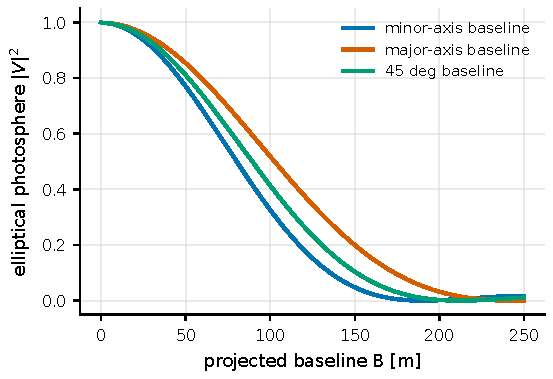
\includegraphics[width=0.82\linewidth]{figures/generated/chapter_10/ch10_rotation_oblateness.pdf}
\caption{快速自转椭圆光球在不同基线方向上的 \(|V|^2\)。参数取 \(\gamma\) Cas 量级的轴比 \(1.28\) 和 \(416~{\rm nm}\) 波长。沿不同位置角投影时有效角直径不同，因此同一基线长度给出的相关强度也不同；这一几何效应使强度干涉能直接测出光球扁率。}
\label{fig:e17-rotation}
\end{figure}

\paragraph{双星：可见度空间里的余弦振荡}
\label{sec:e17-binary}

一对靠得很近、各自都还没被分辨的双星，会在可见度曲线上叠一层余弦波纹。推导很直接：把两颗星当两个点源，主星流量取 1、次星取 \(f\)（流量比），角分离向量 \(\bm{d}\)。两个点源的可见度是各自复相位的加权和，\(V=(1+f\,e^{i\phi})/(1+f)\)，其中相位 \(\phi=2\pi\bm{u}\cdot\bm{d}\) 来自两点源的光程差。取模平方：\(|1+f e^{i\phi}|^2=(1+f\cos\phi)^2+(f\sin\phi)^2=1+f^2+2f\cos\phi\)。除以归一化 \((1+f)^2\)：
\begin{equation}
  |V_{\rm bin}|^2=
  \frac{1+f^2+2f\cos(2\pi\bm{u}\cdot\bm{d})}
       {(1+f)^2}.
  \label{eq:e17-binary}
\end{equation}
\begin{formulaexplain}
\(|V_{\rm bin}|^2\)：未分辨双星的平方可见度。\(f\)：次星与主星的流量比。\(\bm{u}=\bm{B}_\perp/\lambda\)：空间频率。\(\bm{d}\)：角分离向量（弧度）。余弦项让双星在基线空间里振荡。
\end{formulaexplain}
读这条式子：振荡周期由 \(\bm{u}\cdot\bm{d}\) 决定，分离 \(\bm{d}\) 越大、沿基线投影越长，随基线振荡得越快，于是从振荡周期能反推出沿基线方向的角分离；振荡的深浅由 \(f\) 决定，当 \(f\to1\)（两星等亮）时余弦项系数 \(2f/(1+f)^2\to1/2\) 最大，波纹最深，\(f\to0\)（次星极暗）时波纹消失。若两颗星各自还被部分分辨，只需把各自的圆盘可见度式 \eqref{eq:e10-disk} 乘进对应项即可。Narrabri 目录里有些目标后来被认出是双星或多星；现代多基线强度干涉阵列可以把双星轨道、角直径和亮度比联合拟合，再结合径向速度定出质量 \citep{1970MNRAS.148..103H,1974MNRAS.167..121H,2012MNRAS.419..172N}。

\begin{figure}[tbp]
\centering
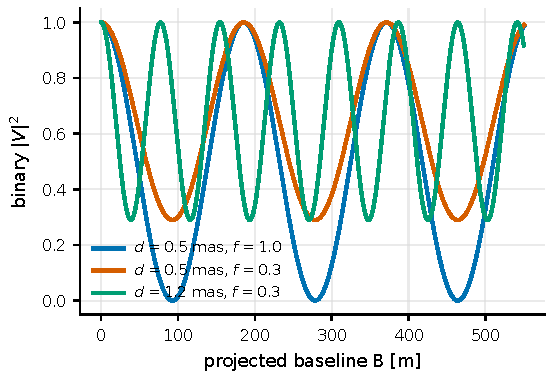
\includegraphics[width=0.82\linewidth]{figures/generated/chapter_10/ch10_binary_visibility.pdf}
\caption{未分辨双星的 \(|V|^2\) 振荡。角分离越大，随基线振荡越快；流量比越接近 1，振荡幅度越大。真实双星还需加入两颗星各自的有限角直径、轨道位置角和多波长流量比。}
\label{fig:e17-binary}
\end{figure}

\paragraph{表面结构：相位缺失带来的退化}
\label{sec:e17-surface}

表面结构比双星更棘手，因为 \(|V|^2\) 缺相位。星斑、对流大颗粒、非径向脉动、Be 星盘都会引入非轴对称的信号；如果只拿一个圆盘或双星模型去套，很可能得到一个"曲线拟合得很漂亮、但物理上是错的"结果——这正是相位缺失导致的模型退化。破解之道是增加约束维度：多基线、多个夜晚、多波长、以及谱线通道，都能各自压掉一部分退化。模拟研究表明，切伦科夫望远镜阵列凭借足够多的基线数和覆盖范围，有机会重建直径、扁率、双星结构乃至大尺度表面特征；但要重建真正复杂的图像，仍需要先验信息或与振幅干涉数据联合 \citep{2012MNRAS.419..172N,2013MNRAS.430.3187R}。

\section{时间变化和谱线通道怎样扩展恒星图像}
\label{sec:e17-time-line}

前面的星都是"静止"的。最后一节让恒星动起来、并让不同波长各说各话，看强度干涉还能多测出什么。

\paragraph{造父变星：把角半径变化接到距离标尺}
\label{sec:e17-cepheid}

造父变星（Cepheid）会周期性地一胀一缩，它的角直径随脉动相位变化。这给了一把独立于视差的量天尺——Baade--Wesselink 类方法。思路是：视向速度谱线告诉我们表面沿视线的运动速度，把它积分就得到半径的物理变化 \(\Delta R\)；而强度干涉直接测角半径的变化 \(\Delta\theta\)。两者之比就是距离。定量地，先约定符号：视向速度 \(v_r\) 以远离我们为正（红移为正），当表面朝我们膨胀时谱线蓝移、\(v_r-v_\gamma<0\)，而此时半径在增大，所以半径变化率与视向脉动速度差一个负号，
\[
  \frac{{\rm d}R}{{\rm d}t}=-p\,[v_r(t)-v_\gamma].
\]
两边对时间积分，得到半径的物理变化
\[
  \Delta R(t)=-\int p\,[v_r(t)-v_\gamma]\,{\rm d}t.
\]
再用角直径与半径的几何关系 \(\Delta\theta=2\Delta R/d\)，代入即得
\begin{equation}
  \Delta\theta(t)=-\frac{2}{d}
  \int p\,[v_r(t)-v_\gamma]\,{\rm d}t .
  \label{eq:e17-baade-wesselink}
\end{equation}
\begin{formulaexplain}
\(\Delta\theta(t)\)：角直径随时间的变化。\(d\)：距离。\(v_r-v_\gamma\)：扣掉整体系统速度后的视向脉动速度（远离为正）。\(p\)：把观测视向速度换算成真实脉动速度的投影因子。负号是速度正方向约定的结果；实际分析只关心 \(\Delta\theta(t)\) 的幅度与相位，符号由约定固定。
\end{formulaexplain}
逐项：\(v_r(t)\) 是谱线测得的视向速度，\(v_\gamma\) 是整颗星相对我们的系统速度（常数），二者之差才是脉动本身。式中的负号纯粹来自"视向速度以远离为正、而膨胀让表面朝我们靠近"这一符号约定；换一套约定负号就会翻面，真正做距离拟合时只用到 \(\Delta\theta(t)\) 曲线的形状（幅度和相位），因此负号不影响结果，但把它写对能保证正文推导和方框公式内部自洽。\(p\) 是投影因子（projection factor），因为谱线是对整个可见半球做视向速度加权平均，而我们要的是表面真实的径向膨胀速度，二者差一个约 \(1.3\) 量级的几何因子。角直径曲线 \(\Delta\theta(t)\) 与速度积分曲线相位匹配后，唯一的自由标度就是 \(d\)，于是距离被定出。系统误差来自 \(p\) 因子、边缘昏暗（脉动中 \(u_\lambda\) 会变）、伴星污染、周期变化和大气速度梯度。明亮造父在可见光强度干涉里特别诱人：它们既亮，半径变化又可预测 \citep{1997A&A...320..799F,2007A&A...476...73F}。

\paragraph{谱线通道：把连续谱和线区的结构分开}
\label{sec:e17-line}

Be 星和 Wolf--Rayet 星的连续谱来自光球，发射线却来自一层延展的星盘或星风，两者空间尺度不同。如果窄带滤光片同时框住连续谱和一条发射线，观测到的可见度是两者按通量加权的和：
\begin{equation}
  V_{\rm obs}=
  \frac{F_{\rm cont}V_{\rm cont}+F_{\rm line}V_{\rm line}}
       {F_{\rm cont}+F_{\rm line}} .
  \label{eq:e17-line-visibility}
\end{equation}
\begin{formulaexplain}
\(V_{\rm obs}\)：窄带内观测到的净可见度。\(F_{\rm cont},F_{\rm line}\)：连续谱与谱线的通量。\(V_{\rm cont},V_{\rm line}\)：各自的可见度。若连续谱已标定，就能反解出谱线形成区的可见度、进而其空间尺度。
\end{formulaexplain}
这条式子的物理根据是两个分量互不相干（mutually incoherent）：连续谱来自光球、发射线来自延展的星盘或星风，两者是不同区域、不同过程发出的光子，彼此没有固定相位关系。互不相干意味着它们的强度直接相加、交叉的干涉项在时间平均下为零，于是互相干函数（也就是可见度）按各自通量线性加权，得到式 \eqref{eq:e17-line-visibility}——无需假设场的相干叠加。用法很实在：先用相邻纯连续谱谱带定出 \(V_{\rm cont}\)（就是光球圆盘），再把它从式 \eqref{eq:e17-line-visibility} 里减掉，就反解出谱线区的 \(V_{\rm line}\)，进而约束星盘半径、倾角或星风几何。对快速旋转的 Be 星，H\(\alpha\) 谱线勾勒星盘，蓝光连续谱勾勒光球；\(\gamma\) Cas 就是范例——强度干涉直接测到光球扁率，而红外或 H\(\alpha\) 干涉补上星盘的几何 \citep{2025ApJ...995..191A}。

最后一类特殊情形是自然激光（astrophysical laser）和受激谱线，可能出现在 \(\eta\) Carinae 这类强辐射场与致密气体团块共存的系统里。要证明某条谱线来自受激辐射，光靠谱线强度不够；需要同时看线宽、空间位置、泵浦通道、偏振，以及谱线通道里的 \(g^{(2)}\)——受激辐射会把光子统计从热光的成群（\(g^{(2)}>1\)）推向相干态的泊松（\(g^{(2)}\to1\)）。第 \ref{chap:e16} 章讨论的自然激光量子诊断，在这里落地成了具体的目标选择清单 \citep{2004A&A...428..497J,2005NewA...10..361J,2008AIPC..984..216D}。

\section{本章要点}
\label{sec:e17-summary}

\begin{itemize}
  \item \textbf{恒星是最稳的标定场。}光球近似热光，亮星光子率足够，角直径在毫角秒量级；强度干涉直接读 \(|V|^2\)（式 \eqref{eq:e17-g2-vis}），不需要望远镜间保持光学相位。模式稀释使实测 \(g^{(2)}(0)-1\) 很小——Vega 零基线只测到 \(1.0034\pm0.0008\)。
  \item \textbf{基线与角尺度同一把尺。}\(B\sim\lambda/\theta\)：可见光下 \(1~{\rm mas}\) 对应约 103 m，\(0.1~{\rm mas}\) 的表面结构需要公里级基线（式 \eqref{eq:e17-baseline}）。
  \item \textbf{角直径加流量给温度。}\(F_{\rm bol}=(\theta_{\rm LD}^2/4)\sigma_{\rm SB}T_{\rm eff}^4\)，距离被约掉（式 \eqref{eq:e17-teff}）；角直径的相对误差在 \(T_{\rm eff}\) 里权重是流量的四倍（式 \eqref{eq:e17-teff-error}）。VERITAS 对 \(\beta\) UMa 得 \(\theta_{\rm LD}=1.07~{\rm mas}\)、\(T_{\rm eff}\simeq9700~{\rm K}\)。
  \item \textbf{边缘昏暗改的是"哪个半径"。}任意轴对称剖面的可见度是 Hankel 变换（式 \eqref{eq:e17-hankel}）；均匀圆盘直径 \(\theta_{\rm UD}\) 与边缘昏暗直径 \(\theta_{\rm LD}\) 可差百分之几，是系统误差而非画图细节。
  \item \textbf{自转、双星、表面结构各有指纹。}扁率让 \(|V|^2\) 随位置角变（式 \eqref{eq:e17-ellipse}，\(\gamma\) Cas 轴比 1.28）；双星叠一层余弦振荡（式 \eqref{eq:e17-binary}）；表面结构因相位缺失易退化，靠多基线、多波长、多夜晚破解。
  \item \textbf{时间与谱线扩展图像。}造父的角半径变化接上 Baade--Wesselink 定距离（式 \eqref{eq:e17-baade-wesselink}）；窄带里连续谱与谱线按通量加权（式 \eqref{eq:e17-line-visibility}），可分出光球与星盘。
\end{itemize}

\noindent\textbf{想一想。}
\begin{itemize}
  \item 一颗 \(0.5~{\rm mas}\) 的亮星，在 \(416~{\rm nm}\) 下第一零点大约在多长基线？（提示：\(B_0\approx1.22\lambda/\theta\)。）若你只有 \(35\)--\(170~{\rm m}\) 基线，你能不能到达零点？到不了对拟合角直径有什么影响？
  \item 若两颗等亮双星（\(f=1\)）的角分离沿某方向为 \(1~{\rm mas}\)，式 \eqref{eq:e17-binary} 的余弦项周期对应多长的基线间隔？把位置角转 \(90^\circ\) 后这个周期会怎样变？
  \item 为什么式 \eqref{eq:e17-teff} 里 \(T_{\rm eff}\) 不依赖距离，而式 \eqref{eq:e17-radius} 里的 \(R\) 和 \(L\) 却依赖？这对"先测温度还是先测半径"的观测策略意味着什么？
\end{itemize}

\chapter{白矮星、中子星与强场物理}
\label{chap:e18}

\begin{chapteropening}
到目前为止，我们打交道的"量子光源"大多是普通恒星：一团热气体，表面温度几千到几万开，发出宽带的热光（第 \ref{chap:e17} 章）。这一章要走到恒星演化的终点站——白矮星（white dwarf）和中子星（neutron star）。它们是把量子物理直接摆到天空上的两个极端标本：白矮星靠电子的\emph{泡利不相容原理}撑着不塌，中子星表面的磁场可以强到让\emph{真空本身}都变成一种有偏振方向的介质。可对我们这些"只会数光子、量相位、测偏振"的观测者来说，它们还带来一个很现实的麻烦：个头太小了。一颗白矮星只有地球那么大，一颗中子星才十几公里——放到几十上百秒差距外，角直径只有微角秒量级，任何单口径望远镜都别想把它"看成一个面"。于是这一章有两条主线拧在一起：一条是\textbf{物理}——简并压、磁层、回旋辐射、真空双折射、表面大气；另一条是\textbf{方法}——既然分辨不了空间结构，我们就改用时间（相位折叠）、能量（能谱）和偏振（Stokes 参量）这三把尺子，把致密天体的信息压进同一张事件表里。这两条线最后都通向后面第 \ref{chap:e22} 章要专门打开的"偏振量子通道"。
\end{chapteropening}


\section{白矮星：电子简并压怎样撑起一颗星}
\label{sec:e18-degeneracy}

先问一个最朴素的问题：一颗恒星烧完了核燃料，没有热核反应再往外顶了，为什么它不干脆一路塌缩成一个点？普通恒星靠的是"热压强"——气体越热，粒子撞得越凶，往外的压力越大。可白矮星已经冷下来了，热运动退居次席。真正顶住引力的，是一种\emph{哪怕温度降到零也不会消失}的压强：电子简并压（electron degeneracy pressure）。它的来历纯粹是量子力学。

物理图像是这样的。把白矮星里的电子想成一群被关在盒子里的乘客，泡利不相容原理（Pauli exclusion principle）规定"一个座位（量子态）最多坐一个（自旋算两个）"。你越是把盒子压小，低能量的座位就越不够坐，后来的电子被迫坐到\emph{动量很高}的座位上去。动量高就意味着运动快、撞墙勤，于是即使一点不加热，这群电子也会拼命往外顶。密度越大，被顶到的动量越高，压强也越大——这就是简并压。

把它写成公式。先算"座位有多满"。在动量空间里，动量小于 \(p\) 的球体体积是 \(\tfrac{4}{3}\pi p^3\)；量子力学告诉我们每个体积为 \(h^3\) 的相空间小格子只能装两个电子（自旋向上、向下各一）。于是单位体积里、动量填到 \(p_F\)（费米动量，Fermi momentum）的电子数密度是
\[
  n_e=\frac{2}{h^3}\cdot\frac{4}{3}\pi p_F^3
     =\frac{8\pi p_F^3}{3h^3}
     =\frac{p_F^3}{3\pi^2\hbar^3},
\]
最后一步用了 \(h=2\pi\hbar\)。反解出费米动量：

\begin{equation}
  p_F=\hbar\,(3\pi^2 n_e)^{1/3},
  \qquad
  n_e=\frac{\rho}{\mu_e m_p}.
  \label{eq:e18-fermi}
\end{equation}
\begin{formulaexplain}
\(p_F\)：费米动量（\(\mathrm{g\,cm\,s^{-1}}\)），电子被填到的最高动量。\(n_e\)：电子数密度（\(\mathrm{cm^{-3}}\)）。\(\rho\)：质量密度；\(\mu_e\)：每个电子摊到的重子数（碳氧星取 \(\simeq2\)）；\(m_p\)：质子质量。密度越高，电子被泡利原理顶得越高。
\end{formulaexplain}

逐符号落地。\(n_e\) 的单位是 \(\mathrm{cm^{-3}}\)；\(\rho\) 是质量密度（\(\mathrm{g\,cm^{-3}}\)）；\(m_p=1.67\times10^{-24}\,\mathrm{g}\)；\(\mu_e\) 之所以出现，是因为白矮星里既有电子也有原子核，每个电子平均"配"了 \(\mu_e\) 个核子的质量，碳氧成分近似 \(\mu_e\simeq2\)。代个真实数字：一颗 \(M\simeq0.6\,M_\odot\)、半径约地球大小（\(R\simeq0.012\,R_\odot\simeq1.3\,R_\oplus\)）的典型 DA 白矮星，平均密度已达 \(10^6\,\mathrm{g\,cm^{-3}}\) 量级，中心可到 \(10^6\)–\(10^9\,\mathrm{g\,cm^{-3}}\)。这个密度是水的百万倍——一茶匙这样的物质有一吨重。

有了 \(p_F\) 就能算压强。理想费米气体的压强来自动量流：\(P=\tfrac13\int_0^{p_F} v(p)\,p\,\dfrac{8\pi p^2}{h^3}\,dp\)，其中 \(\tfrac13\) 是三个方向平摊的几何因子，\(v(p)\) 是动量为 \(p\) 的电子速度。当电子跑得比光慢很多（\(p_F\ll m_ec\)），\(v=p/m_e\)，积分是
\[
  P_{\rm NR}=\frac{8\pi}{3h^3m_e}\int_0^{p_F}p^4\,dp
           =\frac{8\pi\,p_F^5}{15h^3m_e}
           =\frac{p_F^5}{15\pi^2\hbar^3 m_e}.
\]
把 \(\eqref{eq:e18-fermi}\) 的 \(p_F\) 代进去、整理指数，得到

\begin{equation}
  P_{\rm NR}=\frac{(3\pi^2)^{2/3}}{5}\,
             \frac{\hbar^2}{m_e}\,n_e^{5/3}.
  \label{eq:e18-pnr}
\end{equation}
\begin{formulaexplain}
\(P_{\rm NR}\)：非相对论电子简并压（\(\mathrm{dyn\,cm^{-2}}\)），随密度以 \(n_e^{5/3}\) 上冲。这是一支"很硬"的支撑：密度稍升，压强猛增，普通白矮星就靠它顶住引力。
\end{formulaexplain}

请留意那个指数 \(5/3\)。它意味着这支压强"很硬"——你想再压小一点，它就用力得多的反抗。这就是为什么低质量白矮星能安安稳稳地存在几十亿年。

可是质量一大，麻烦就来了。质量越大、压得越紧、\(n_e\) 越高，费米动量就可能超过 \(m_ec\)：电子被顶到\emph{接近光速}。这时 \(v\to c\) 不再是 \(p/m_e\)，速度被光速卡住涨不上去了。把 \(v=c\) 代进同一个压强积分：
\[
  P_{\rm ER}=\frac{8\pi c}{3h^3}\int_0^{p_F}p^3\,dp
           =\frac{2\pi c\,p_F^4}{3h^3}
           =\frac{c\,p_F^4}{12\pi^2\hbar^3},
\]
再代 \(p_F\)：

\begin{equation}
  P_{\rm ER}=\frac{(3\pi^2)^{1/3}}{4}\,\hbar c\,n_e^{4/3}.
  \label{eq:e18-per}
\end{equation}
\begin{formulaexplain}
\(P_{\rm ER}\)：极端相对论电子简并压，密度指数软化为 \(4/3\)。支撑变软后，质量再加，半径急剧缩小——这是走向 Chandrasekhar 极限的物理根源。
\end{formulaexplain}

现在指数从 \(5/3\) 降到了 \(4/3\)。这一降是致命的：压强对密度的响应变"软"了，你再往上加质量，它顶不住多少。极端情形下引力和简并压的密度指数打平，星体失去稳定支撑——这就是 Chandrasekhar 极限（Chandrasekhar mass）的物理来源 \citep{1931ApJ....74...81C,1935MNRAS..95..207C,1961ApJ...134..683H}。

把上面的标度关系接到观测者能用的形式，常写成 Nauenberg 的质量–半径近似：

\begin{equation}
  R\simeq 0.0112\,R_\odot
  \left[\left(\frac{M_{\rm Ch}}{M}\right)^{2/3}
  -\left(\frac{M}{M_{\rm Ch}}\right)^{2/3}\right]^{1/2},
  \qquad
  M_{\rm Ch}\simeq 5.83\,\mu_e^{-2}\,M_\odot .
  \label{eq:e18-nauenberg}
\end{equation}
\begin{formulaexplain}
\(R\)：白矮星半径；\(M\)：质量；\(M_{\rm Ch}\)：Chandrasekhar 极限质量（\(\mu_e=2\) 时约 \(1.46\,M_\odot\)）。\(M\to M_{\rm Ch}\) 时方括号趋零，半径塌向零——"越重越小"。
\end{formulaexplain}

这个式子把\eqref{eq:e18-pnr}、\eqref{eq:e18-per}两支压强合成一条曲线。它假设零温、不转、无强磁场形变，适合估算 \(0.2\)–\(1.35\,M_\odot\) 白矮星的主标度。请注意它和普通恒星\emph{相反}的脾气：普通恒星越重越大，白矮星却越重越小。真实半径还受核心成分、氢氦包层厚度、有限温度和磁场影响，高精度工作要靠演化模型或双星约束 \citep{1972ApJ...175..417N,2017MNRAS.470.4473P,2020ApJ...899..146C}。图~\ref{fig:e18-wd-mr} 把这条"越重越小"的曲线画了出来。

\begin{figure}[tbp]
\centering
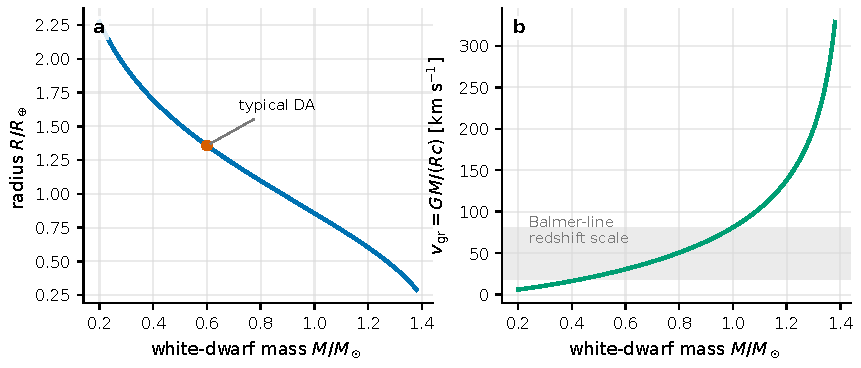
\includegraphics[width=0.94\linewidth]{figures/generated/chapter_11/ch11_white_dwarf_mass_radius.pdf}
\caption{白矮星质量增加时半径变小，靠近 Chandrasekhar 极限时收缩更快。右图把同一质量–半径关系换成光谱中可测的引力红移速度 \(v_{\rm gr}=GM/(Rc)\)，典型 DA 白矮星的 Balmer 线红移是几十 \(\mathrm{km\,s^{-1}}\)，已经接近或超过普通恒星大气运动的速度尺度。}
\label{fig:e18-wd-mr}
\end{figure}


\section{小角尺度：致密天体为什么这么难"看清"}
\label{sec:e18-angsize}

上一节算出白矮星大概只有地球那么大。这一节把这个"小"翻译成观测者最怕的一个量：角直径（angular diameter）。回忆第 \ref{chap:e11} 章讲成像时的定义——一个真实直径为 \(2R\)、距离 \(d\) 的圆盘，张开的角是

\begin{equation}
  \theta_{\rm WD}=\frac{2R}{d}
  \simeq 11\,\mu\mathrm{as}
  \left(\frac{R}{0.012\,R_\odot}\right)
  \left(\frac{10\,\mathrm{pc}}{d}\right).
  \label{eq:e18-theta}
\end{equation}
\begin{formulaexplain}
\(\theta_{\rm WD}\)：白矮星角直径（微角秒 \(\mu\mathrm{as}\)）；\(R\)：半径；\(d\)：距离。即使近到 \(10\,\mathrm{pc}\)，也只有约 \(11\,\mu\mathrm{as}\)——远在单口径望远镜的分辨能力之外。
\end{formulaexplain}

把数字摆出来体会一下。\(1\,\mathrm{rad}=2.06\times10^{11}\,\mu\mathrm{as}\)；\(10\,\mathrm{pc}=3.1\times10^{19}\,\mathrm{cm}\)，\(R=0.012\,R_\odot=8.3\times10^8\,\mathrm{cm}\)。于是 \(\theta=2R/d\approx5.3\times10^{-11}\,\mathrm{rad}\approx11\,\mu\mathrm{as}\)。对照第 \ref{chap:e12} 章：一台 8 米镜在可见光的 Rayleigh 角约 \(16\,\mathrm{mas}=1.6\times10^4\,\mu\mathrm{as}\)（换算用 \(1\,\mathrm{mas}=10^3\,\mu\mathrm{as}\)）——比这颗白矮星大了约三个数量级（\(1.6\times10^4/11\approx1.5\times10^3\)）。就算换 30 米巨镜，Rayleigh 角只缩到约 \(4.3\,\mathrm{mas}\approx4.3\times10^3\,\mu\mathrm{as}\)，仍差两到三个数量级。结论很硬：\textbf{致密天体的空间结构，单口径成像基本无望}。

那怎么办？有两条出路，恰好都是本书前半部搭好的舞台。第一条是把基线拉长——第 \ref{chap:e10} 章的强度干涉（intensity interferometry）测的是两台相距 \(B\) 的望远镜之间的二阶相干 \(g^{(2)}\)，等效分辨本领是 \(\lambda/B\)。要把 \(11\,\mu\mathrm{as}\) 分辨出来，需要 \(B\sim\lambda/\theta\sim5\times10^{-5}\,\mathrm{cm}/5\times10^{-11}\approx10^6\,\mathrm{cm}=10\,\mathrm{km}\) 量级的基线——这正是第 \ref{chap:e22}、\ref{chap:e24} 章工程方案要够的尺度。第二条出路更省事：既然分辨不了"面"，那就别硬碰空间，改去挖\emph{时间}和\emph{偏振}里的信息。致密天体转得快、磁场强，把结构信息大量编码在光变相位和偏振里——这正是本章后面几节的主战场。

顺带说一个"不用分辨就能量物理"的漂亮例子：引力红移。光子从强引力势阱里爬出来会损失能量、波长变长，等效成一个视向速度

\begin{equation}
  v_{\rm gr}=\frac{GM}{Rc}
  \simeq 31.8\,\mathrm{km\,s^{-1}}
  \left(\frac{M}{0.6\,M_\odot}\right)
  \left(\frac{0.012\,R_\odot}{R}\right).
  \label{eq:e18-vgr}
\end{equation}
\begin{formulaexplain}
\(v_{\rm gr}\)：引力红移等效速度，正比于 \(M/R\)（即紧致度）。谱线红移因此把质量–半径关系变成一个可测的速度——不需要分辨星面。
\end{formulaexplain}

推导只有一步：广义相对论给出的分数红移是 \(\Delta\lambda/\lambda\simeq GM/(Rc^2)\)（弱场极限），乘以 \(c\) 就是等效速度 \(v_{\rm gr}=GM/(Rc)\)。它把"越重越小"（\eqref{eq:e18-nauenberg}）的白矮星翻译成谱线上几十 \(\mathrm{km\,s^{-1}}\) 的位移，已经超过普通恒星大气的运动速度，因此可测。当然实测要扣掉系统本动速度、对流线移和 Stark 位移，所以大样本工作常把 Gaia 半径、SDSS 光谱线心和运动学模型一起平均。图~\ref{fig:e18-wd-mr} 右图正是这条"半径换速度"的映射。


\section{磁白矮星：吸积几何怎样写进相位和偏振}
\label{sec:e18-mcv}

有一类白矮星带着强磁场：孤立磁白矮星表面场从 \(10^6\) 到 \(10^9\,\mathrm{G}\)，吸积双星（激变变星，cataclysmic variable）里的极（polar）和中介极（intermediate polar）常见 \(1\)–\(200\,\mathrm{MG}\)。这里磁场不再是配角，它直接把结构问题和光子统计问题拧在一起。先给磁场一个"作用半径"。一个磁偶极子的磁矩是场强乘以半径立方：

\begin{equation}
  \mu = B_* R_{\rm WD}^3
  \simeq 5.1\times10^{33}\,\mathrm{G\,cm^3}
  \left(\frac{B_*}{10\,\mathrm{MG}}\right)
  \left(\frac{R_{\rm WD}}{8\times10^8\,\mathrm{cm}}\right)^3 .
  \label{eq:e18-mu}
\end{equation}
\begin{formulaexplain}
\(\mu\)：磁矩（\(\mathrm{G\,cm^3}\)）；\(B_*\)：表面磁场；\(R_{\rm WD}\)：半径。磁矩越大，磁场就能在离星更远的地方接管吸积流。
\end{formulaexplain}

为什么要算磁矩？因为落向白矮星的气体是电离的，带电粒子只能沿磁力线走。当磁场的能量密度足以主导流的动能时，气流就被"接管"、被迫顺着磁力线拐向磁极。这个接管发生的半径叫磁层半径（magnetospheric radius）：

\begin{equation}
  r_m \simeq k
  \left(\frac{\mu^4}{2GM\dot M^2}\right)^{1/7},
  \label{eq:e18-rm}
\end{equation}
\begin{formulaexplain}
\(r_m\)：磁层半径；\(k\sim0.5\)–\(1\) 是几何因子；\(\dot M\)：吸积率。磁矩越大把磁层推得越远，吸积率越高把磁层压得越近。
\end{formulaexplain}

那个 \(1/7\) 次幂看着古怪，其实来自"磁压等于落流冲压"的平衡：磁压 \(\propto B^2\propto\mu^2/r^6\)，落流冲压 \(\propto\dot M\sqrt{GM/r}/r^2\propto r^{-5/2}\)，两边令相等解出 \(r_m\propto(\mu^4/GM\dot M^2)^{1/7}\)——指数 \(4\)、\(1\)、\(2\) 和 \(7\) 全是这么配平出来的。激变变星的 \(\dot M\) 从 \(10^{-11}\) 到 \(10^{-8}\,M_\odot\,\mathrm{yr^{-1}}\) 不等，磁层大小随之在星面附近到几十倍星半径之间浮动。

磁层大小要和另一个半径比才有意义——共转半径（corotation radius），也就是磁场随星刚性共转的角速度恰好等于开普勒轨道角速度的地方：

\begin{equation}
  r_{\rm co}=\left(\frac{GM}{\Omega_s^2}\right)^{1/3},
  \label{eq:e18-rco}
\end{equation}
\begin{formulaexplain}
\(r_{\rm co}\)：共转半径；\(\Omega_s\)：白矮星自转角速度。此处"磁场拉着转"的速度与"引力允许的绕转"速度打平，是吸积能否顺利落下的分水岭。
\end{formulaexplain}

它的推导也是一步：令共转线速度对应的离心力 \(\Omega_s^2 r\) 等于引力 \(GM/r^2\)，解出 \(r_{\rm co}=(GM/\Omega_s^2)^{1/3}\)。物理判据很直观：若 \(r_m<r_{\rm co}\)，物质在共转半径以内被磁场接手，可以较顺当地沿磁力线落到磁极；若 \(r_m\gtrsim r_{\rm co}\)，磁力线在接手处已经转得比开普勒还快，会\emph{甩}物质，形成"螺旋桨"式的抛射或改变流形态。观测上，中介极的 \(P_{\rm spin}/P_{\rm orb}\) 常在 \(0.01\)–\(0.6\)，而极几乎同步（\(P_{\rm spin}\simeq P_{\rm orb}\)）\citep{1970ApJ...160L.147A,2000PASP..112..873W,1991MNRAS.249..460W,2008ApJ...672..524N}。图~\ref{fig:e18-mcv-map} 把这套"磁矩与自转快慢决定几何"的分类画了出来。

\begin{figure}[tbp]
\centering
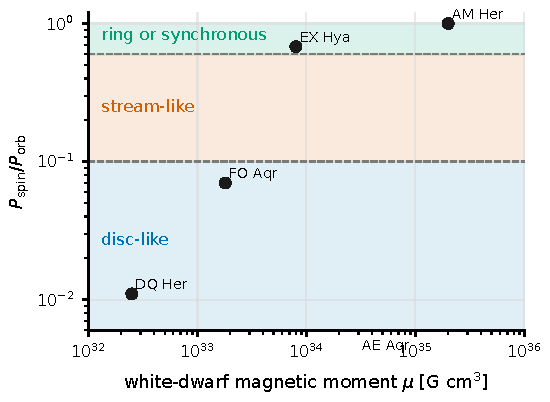
\includegraphics[width=0.78\linewidth]{figures/generated/chapter_11/ch11_magnetic_cv_flow_map.pdf}
\caption{磁激变变星的吸积流主要由白矮星磁矩和自转相对轨道的快慢决定。低 \(P_{\rm spin}/P_{\rm orb}\) 系统容易形成盘状流，中间区域常出现磁控流，接近同步或高比值系统会转向环状、流状或极系统几何；这些几何会直接改变光变相位、圆偏振和相关函数。}
\label{fig:e18-mcv-map}
\end{figure}

流落下来会释放引力势能，转成光。数量级由势阱深度乘以质量流率给出：

\begin{equation}
  L_{\rm acc}\simeq \frac{GM\dot M}{R_{\rm WD}}
  \simeq 1.0\times10^{33}\,\mathrm{erg\,s^{-1}}
  \left(\frac{M}{0.8\,M_\odot}\right)
  \left(\frac{\dot M}{10^{-10}M_\odot\,\mathrm{yr^{-1}}}\right)
  \left(\frac{8\times10^8\,\mathrm{cm}}{R_{\rm WD}}\right).
  \label{eq:e18-lacc}
\end{equation}
\begin{formulaexplain}
\(L_{\rm acc}\)：吸积光度（\(\mathrm{erg\,s^{-1}}\)），等于单位时间释放的引力势能 \(GM\dot M/R\)。它给出这类系统可用光子率的数量级；光学只接收其中一部分。
\end{formulaexplain}

这份光度是各种成分的混合：吸积盘、磁极附近的热斑、柱状冲击区、被照亮的白矮星面，以及\emph{回旋辐射}（cyclotron emission）。这里就接上了本章的一个教学重点——强磁场怎样把偏振写进光里。带电电子在磁场里会绕着磁力线打转，转动的角频率是回旋频率（cyclotron frequency）
\[
  \omega_c=\frac{eB}{m_e c},
  \qquad
  \hbar\omega_c\approx 11.6\,\mathrm{keV}\left(\frac{B}{10^{12}\,\mathrm{G}}\right).
\]
电子转圈就是一个加速的电荷，会辐射；辐射集中在 \(\omega_c\) 及其谐波上。对磁白矮星 \(B\sim10\)–\(200\,\mathrm{MG}=10^7\)–\(2\times10^8\,\mathrm{G}\)，基频光子能量 \(\hbar\omega_c\sim0.1\)–\(2\,\mathrm{eV}\)，加上若干谐波，正好落在近红外到光学——这就是为什么极的光学光变里会鼓起一串"回旋驼峰"。关键在于：电子绕磁力线转，辐射天然带\emph{偏振}——你顺着磁力线看到的是圆偏振，侧着看到的是线偏振。于是偏振成了把回旋成分从盘光、黑体光里\emph{挑出来}的探针。（把非相对论的回旋辐射换成相对论电子，就是第 \ref{chap:e16} 章讲过的同步辐射 synchrotron，两者是同一机制在不同能段的两副面孔。）

偏振怎么读几何？两条经验规则很好用。其一，圆偏振的\emph{符号}如果随自转相位翻转，通常意味着视线扫过了不同的磁极、或磁场投影方向变了号。其二，线偏振峰和总光变峰如果\emph{不同步}，说明"最亮的区域"和"磁场几何最特殊的区域"不是同一块——强度峰来自冲击区加热，偏振峰来自磁场投影。

这些相位调制该怎样在事件表里定量？把光子按白矮星自转相位 \(\phi_s\) 分箱，在每个相位窗内算二阶强度相关（第 \ref{chap:e08} 章的 \(g^{(2)}\)）：

\begin{equation}
  g^{(2)}_{\phi_s}(\tau)=
  \frac{\langle I_{\phi_s}(t)\,I_{\phi_s}(t+\tau)\rangle}
       {\langle I_{\phi_s}(t)\rangle^2}.
  \label{eq:e18-g2phi}
\end{equation}
\begin{formulaexplain}
\(g^{(2)}_{\phi_s}(\tau)\)：固定自转相位窗 \(\phi_s\) 内的二阶强度相关；\(I_{\phi_s}\)：该窗内的计数率。它抽取同一磁极或同一段吸积流在延迟 \(\tau\) 上的"短时记忆"。
\end{formulaexplain}

读法要小心时间尺度。若 \(\tau\) 在毫秒到秒，\(g^{(2)}\) 的结构可能来自冲击区冷却、磁控团块，或者纯属探测器死时间的假信号；若 \(\tau\) 在几十秒到分钟，则更像经典的闪烁（flickering）或大气透明度起伏，而非致密源本身。还有一条铁律：\eqref{eq:e18-g2phi} 里的平均\emph{必须}在同一相位窗、同一能段、同一偏振通道内做，否则轨道调制会被误当成短时相关——这正是"相位分辨"四个字的分量所在。


\section{中子星：磁层怎样切成一张相位事件表}
\label{sec:e18-nsphase}

中子星比白矮星还小一个数量级：半径只有 \(10\)–\(14\,\mathrm{km}\)，质量却常在 \(1.2\)–\(2.2\,M_\odot\)。这么小的天体转得飞快、磁场极强，于是它的磁层被自转"切"成了一套天然的相位坐标。最基本的一条界线是光柱半径（light cylinder radius）——刚性共转的线速度恰好达到光速的地方：

\begin{equation}
  R_{\rm LC}=\frac{c}{\Omega}=\frac{cP}{2\pi}
  \simeq 1.6\times10^3\,\mathrm{km}
  \left(\frac{P}{33\,\mathrm{ms}}\right).
  \label{eq:e18-rlc}
\end{equation}
\begin{formulaexplain}
\(R_{\rm LC}\)：光柱半径；\(P\)：自转周期；\(\Omega=2\pi/P\)：角速度。此处 "跟着星刚性共转" 需要达到光速，因此它是开放磁力线、粒子加速与高能辐射能组织的最外边界。
\end{formulaexplain}

推导只有一句话：共转线速度 \(v=\Omega r\) 令其等于 \(c\)，解出 \(r=c/\Omega=cP/2\pi\)。数量级很有画面感：Crab 脉冲星 \(P\simeq33\,\mathrm{ms}\)，光柱约 \(1600\,\mathrm{km}\)；毫秒脉冲星 \(P\simeq1.5\)–\(10\,\mathrm{ms}\)，光柱只有几十到几百公里；磁星（magnetar）\(P\simeq2\)–\(12\,\mathrm{s}\)，光柱可达 \(10^5\,\mathrm{km}\) 以上。在 \(R_{\rm LC}\) 以内的磁力线闭合、随星共转；越过它就得开放，粒子沿开放磁力线加速、辐射。脉冲星的发现和"旋转中子星"解释确立了这幅图像，Crab 又把旋转能损失和超新星遗迹联系起来 \citep{1968Natur.217..709H,1968Natur.218..731G,1968Natur.219..145P,1972ApJ...175..217B}。图~\ref{fig:e18-lc} 画出光柱随周期的线性增长和 Crab 型相位轮廓。

\begin{figure}[tbp]
\centering
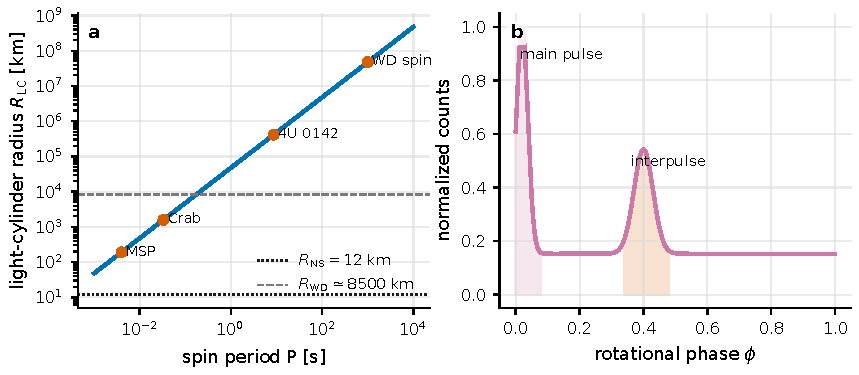
\includegraphics[width=0.94\linewidth]{figures/generated/chapter_11/ch11_light_cylinder_phase.pdf}
\caption{光柱半径随自转周期线性增加。毫秒脉冲星的光柱只有几十到几百公里，Crab 约 \(1.6\times10^3\,\mathrm{km}\)，磁星则可到 \(10^5\,\mathrm{km}\) 以上。右图是 Crab 型相位折叠轮廓，主脉冲和 interpulse 的相位窗决定哪些光子进入后续的强度相关或偏振统计。}
\label{fig:e18-lc}
\end{figure}

磁场强到什么程度？我们量不到中子星表面，但可以从它转得越来越慢反推。一个磁化的转动天体像个天线，向外辐射磁偶极波、带走能量，于是自转减慢。这一步的中间桥梁是磁偶极辐射公式：一个磁矩为 \(m=B R^3\)、以角速度 \(\Omega\) 转动、磁轴与自转轴夹角为 \(\chi\) 的偶极子，向外辐射的功率是（经典 Larmor 公式对旋转磁偶极的推广）
\[
  \dot E_{\rm dip}=\frac{B^2R^6\Omega^4\sin^2\chi}{6c^3}.
\]
让这份辐射损耗等于自转动能的损失 \(\dot E=I\Omega\dot\Omega\)（下一式\eqref{eq:e18-edot}会展开），两边令相等、解出 \(B\)，再代入标准假设 \(R=10\,\mathrm{km}\)、\(I=10^{45}\,\mathrm{g\,cm^2}\)、\(\sin\chi=1\)，并把 \(\Omega=2\pi/P\)、\(\dot\Omega=-2\pi\dot P/P^2\) 换成周期，就整理出赤道表面磁场

\begin{equation}
  B_{\rm dip}\simeq 3.2\times10^{19}\,(P\dot P)^{1/2}\,\mathrm{G}.
  \label{eq:e18-bdip}
\end{equation}
\begin{formulaexplain}
\(B_{\rm dip}\)：由自转慢化推出的偶极磁场（\(\mathrm{G}\)）；\(P\) 用秒，\(\dot P\)（无量纲 \(\mathrm{s\,s^{-1}}\)）是周期的变化率。它把计时数据里的"越转越慢"翻译成磁场标度。
\end{formulaexplain}

数字告诉我们中子星磁场有多离谱：普通年轻脉冲星 \(B_{\rm dip}\sim10^{11}\)–\(10^{13}\,\mathrm{G}\)，磁星可到 \(10^{14}\)–\(10^{15}\,\mathrm{G}\)——地球磁场才 \(0.5\,\mathrm{G}\)，最强的实验室稳态磁场也不过 \(10^5\,\mathrm{G}\) 量级。这个磁场后面就是真空双折射的舞台。慢化释放的能量率是

\begin{equation}
  \dot E = 4\pi^2 I\,\frac{\dot P}{P^3},
  \qquad
  I\simeq10^{45}\,\mathrm{g\,cm^2}.
  \label{eq:e18-edot}
\end{equation}
\begin{formulaexplain}
\(\dot E\)：自转能损失率（\(\mathrm{erg\,s^{-1}}\)）；\(I\)：转动惯量（约 \(10^{45}\,\mathrm{g\,cm^2}\)）。它是脉冲星驱动磁层辐射和星云的总能量预算。
\end{formulaexplain}

推导：自转动能 \(E=\tfrac12 I\Omega^2=2\pi^2 I/P^2\)，对时间求导 \(\dot E=-4\pi^2 I\dot P/P^3\)（取正号表示损耗率）。Crab 的 \(\dot E\sim10^{38}\,\mathrm{erg\,s^{-1}}\)，足以点亮从射电到 \(\gamma\) 射线的脉冲和整个 Crab 星云 \citep{1984ApJ...283..279H,1992ApJ...397..187B,2001A&A...378..918K,2008ApJ...680.1378H}。

现在把光子送进相位坐标。每个光子先做太阳系质心改正（把地球公转造成的到达时间差扣掉），再用计时星历折叠成相位：

\begin{equation}
  \phi_i=
  \left[
  \nu(t_i-t_0)+\tfrac12\dot\nu(t_i-t_0)^2
  +\tfrac16\ddot\nu(t_i-t_0)^3+\cdots
  \right]\bmod 1 .
  \label{eq:e18-fold}
\end{equation}
\begin{formulaexplain}
\(\phi_i\)：第 \(i\) 个光子的自转相位（\(0\)–\(1\)）；\(t_i\)：其质心到达时刻；\(\nu=1/P\) 及 \(\dot\nu,\ddot\nu\)：自转频率与其导数。取 \(\bmod\,1\) 把绵长的到达时间表卷成一圈相位。
\end{formulaexplain}

逐项看：\(t_i\) 是质心时刻（秒），\(t_0\) 是参考历元，\(\nu\) 描述基本自转，\(\dot\nu\) 描述慢化，\(\ddot\nu\) 描述 glitch 后的恢复等高阶项。这一步把"一长串到达时刻"卷成"一圈 \(0\) 到 \(1\) 的相位"，多圈叠加就得到高信噪比的脉冲轮廓（图~\ref{fig:e18-lc} 右）。Crab 的主脉冲宽度只占相位约 \(0.04\)–\(0.05\)，射电巨脉冲（giant radio pulse）能窄到微秒。有意思的是：把巨射电脉冲发生的那些周期挑出来，光学主脉冲平均会增强约 \(3\%\)，而脉冲形状和到达相位基本不变；ARCONS 的能量分辨光子计数进一步显示，早到的巨射电脉冲对应的光学增强可达十几到二十几个百分点 \citep{2003Sci...301..493S,2013ApJ...779L..12S}。这些结果把相干的射电爆发和非相干的光学辐射接到了同一部分磁层等离子体上——一个只有把射电和光学放进\emph{同一张相位事件表}才看得见的联系。

有了相位坐标，就能做相位分辨的二阶相关，把不同能段、偏振或望远镜在同一脉冲相位上的同步涨落比出来：

\begin{equation}
  g^{(2)}_{ab}(\tau\mid\Phi)=
  \frac{\langle n_a(t,\Phi)\,n_b(t+\tau,\Phi)\rangle}
       {\langle n_a(t,\Phi)\rangle\langle n_b(t,\Phi)\rangle},
  \label{eq:e18-g2ab}
\end{equation}
\begin{formulaexplain}
\(g^{(2)}_{ab}(\tau\mid\Phi)\)：相位窗 \(\Phi\) 内、通道 \(a\) 与 \(b\) 的互相关；\(n_a,n_b\)：两通道计数。\(a,b\) 可以是能段、偏振或不同望远镜，用来看同一脉冲相位上的同步性。
\end{formulaexplain}

对 Crab 这样的亮源，\(\tau\) 能推进到微秒至毫秒，真正逼近单脉冲统计；对更暗的光学脉冲星，最先能做的通常还只是相位窗内的光度和偏振堆叠，离逐脉冲相关还有距离 \citep{1996ApJ...468..779M,2000ApJ...537..861S,2009MNRAS.397..103S}。这里 \(a,b\) 走向不同望远镜时，\eqref{eq:e18-g2ab} 就直接接上了第 \ref{chap:e10} 章的强度干涉——只不过现在每个 \(g^{(2)}\) 都挂在一个自转相位标签上。


\section{强磁场偏振：真空双折射与 QED 强场效应的印记}
\label{sec:e18-qed}

这一节走到本章物理上最"量子"的地方。经典电动力学里，真空是空的、不弯光、不分偏振。可量子电动力学（QED）说：真空里其实翻涌着虚电子–正电子对，强磁场会把它们\emph{极化}，让真空变成一种有偏振方向的介质——就像方解石晶体那样双折射。这个效应叫真空双折射（vacuum birefringence）。它什么时候变强？标尺是 QED 临界磁场（critical field）：

\begin{equation}
  B_Q=\frac{m_e^2c^3}{e\hbar}=4.414\times10^{13}\,\mathrm{G}.
  \label{eq:e18-bq}
\end{equation}
\begin{formulaexplain}
\(B_Q\)：QED 临界磁场。在这个场强下，电子最低朗道能级的回旋能量已接近它的静止能 \(m_ec^2\)，量子磁效应不再是小修正。磁星表面 \(B\) 逼近甚至超过 \(B_Q\)。
\end{formulaexplain}

\(B_Q\) 的物理意义值得咂摸：把 \(\hbar\omega_c=\hbar eB/(m_ec)\) 令其等于电子静能 \(m_ec^2\)，解出的正是 \(B=m_e^2c^3/(e\hbar)=B_Q\)。也就是说，当磁场强到"电子转一圈的量子能量就等于它整个静止质量"，真空的量子结构就不能忽略了。磁星表面 \(B\sim10^{14}\)–\(10^{15}\,\mathrm{G}\)，比 \(B_Q\) 还大一个量级——真空双折射在这里不是纸上谈兵。

当 \(B\ll B_Q\) 且光子能量远低于 \(m_ec^2\) 时，Heisenberg–Euler 有效理论给出两个偏振正常模之间的折射率差（弱场近似）：

\begin{equation}
  \Delta n\simeq\frac{\alpha_{\rm fs}}{30\pi}
  \left(\frac{B_\perp}{B_Q}\right)^2 ,
  \label{eq:e18-dn}
\end{equation}
\begin{formulaexplain}
\(\Delta n\)：平行与垂直两个偏振正常模的折射率之差；\(B_\perp\)：垂直于光线的磁场分量；\(\alpha_{\rm fs}\simeq1/137\)：精细结构常数。它随 \(B_\perp^2\) 增长——磁场加倍，双折射变四倍。
\end{formulaexplain}

注意 \(\Delta n\propto B_\perp^2\)：磁场是这个效应的"油门"，而且踩得很猛。磁星表面场超过 \(B_Q\)，弱场公式已不能当精确模型用，但它点破了要害——\emph{偏振对强场极其敏感}。两个偏振模在真空里以略微不同的速度传播，沿光路积累出相位差：

\begin{equation}
  \Delta\Phi(E)=\frac{E}{\hbar c}\int\Delta n(s)\,ds .
  \label{eq:e18-dphi}
\end{equation}
\begin{formulaexplain}
\(\Delta\Phi(E)\)：两个偏振模积累的相位差；\(E\)：光子能量；积分沿光路 \(s\) 进行。能量越高、路径上 \(\Delta n\) 越大，偏振传播效应越强。
\end{formulaexplain}

这个相位差带来一个可观测的后果，叫偏振冻结（polarization freezing）。想象光子从磁星表面不同小块出发，每块的磁场方向不同、偏振方向也不同。如果没有真空双折射，这些方向乱七八糟的偏振光叠在一起会互相抵消，观测到的净偏振度很低。可有了双折射，只要传播是绝热的，偏振矢量会\emph{锁定}在局部磁场方向上、随磁场缓慢转动，一直到很远处的"偏振限制半径"才冻结下来。结果是：来自星面大片区域的偏振方向被磁场"梳"到一致，抵消减少，净偏振度反而\emph{升高}。所以\textbf{一个高偏振度本身，就是真空双折射的间接印记}。这套图像来自强场 QED、磁层传播和中子星表面辐射模型的组合 \citep{1936ZPhy...98..714H,1971AnPhy..67..599A,2000MNRAS.311..555H,2002PhRvD..66b3002H,2003MNRAS.342..134H}。X 射线偏振仪（如 IXPE）在 \(2\)–\(8\,\mathrm{keV}\) 工作，正是要在这个能段测这份偏振。

那"偏振度"和"偏振角"到底怎么从光子里算出来？这是本章和第 \ref{chap:e22} 章共用的核心工具。X 射线偏振仪对每个光电事件测出一个方位角（调制角，modulation angle）\(\eta_i\)，然后把许多事件累加成 Stokes 参量（Stokes parameters）（下式的总强度 \(I\) 与\eqref{eq:e18-edot}的转动惯量 \(I\) 同符不同义，请勿混淆）：

\begin{equation}
  I=\sum_i w_i,\qquad
  Q=\sum_i w_i\cos 2\eta_i,\qquad
  U=\sum_i w_i\sin 2\eta_i .
  \label{eq:e18-stokes}
\end{equation}
\begin{formulaexplain}
\(I\)：总强度；\(Q,U\)：两个线偏振 Stokes 分量；\(\eta_i\)：第 \(i\) 个事件的方位角；\(w_i\)：权重（含仪器调制、背景、有效面积因子）。角度前的因子 \(2\) 反映偏振是"无向"的——转 \(180^\circ\) 回到自身。
\end{formulaexplain}

为什么是 \(\cos2\eta\) 而不是 \(\cos\eta\)？因为偏振是一条\emph{无方向的线}：偏振方向转 \(180^\circ\) 和没转一样，所以物理量必须以 \(2\eta\) 为周期。把大量事件的方位角这样加权求和，随机方向的会互相抵消，只有真正偏振的方向会在 \(Q,U\) 上留下净矢量。由它得到偏振度和偏振角：

\begin{equation}
  p=\frac{\sqrt{Q^2+U^2}}{I},\qquad
  \psi=\tfrac12\arctan2(U,Q).
  \label{eq:e18-pdop}
\end{equation}
\begin{formulaexplain}
\(p\)：线偏振度（\(0\)–\(1\)）；\(\psi\)：偏振角。\((Q,U)\) 这个二维矢量的\emph{长度}给偏振强弱，\emph{方向}（除以 2 后）给天空上的偏振角。
\end{formulaexplain}

代个真实数字：光学偏振测量孤立中子星 RX J1856.5\(-\)3754 得到 \(p=16.43\%\pm5.26\%\)，而源本身暗到 \(V\simeq25.5\)——前景星际偏振和仪器偏振都要逐项扣。这样一个偏高的偏振度，和热表面模型对照，支持真空双折射减少了不同表面区域的偏振相消 \citep{2015MNRAS.454.3254T,2016MNRAS.459.3585G,2017MNRAS.465..492M}。图~\ref{fig:e18-stokes} 展示旋转磁几何怎样把偏振投影成 \(Q/I\)、\(U/I\) 的相位曲线和 Q–U 平面上的轨迹。

\begin{figure}[tbp]
\centering
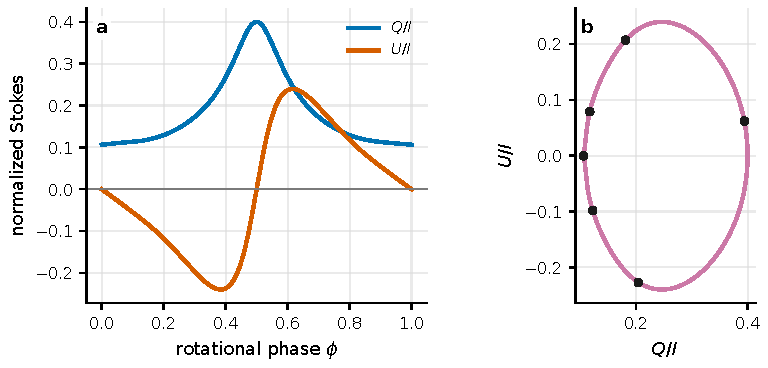
\includegraphics[width=0.92\linewidth]{figures/generated/chapter_11/ch11_stokes_qu_track.pdf}
\caption{旋转磁几何会把偏振角变化投影成 \(Q/I\) 和 \(U/I\) 的相位曲线。左图显示同一相位事件表给出的两个 Stokes 分量，右图显示对应的 Q--U 轨迹；轨迹形状比单独的偏振度更能暴露几何退化和仪器串扰。}
\label{fig:e18-stokes}
\end{figure}

偏振角随相位怎么摆？第一近似用旋转矢量模型（rotating vector model）：

\begin{equation}
  \tan(\psi-\psi_0)=
  \frac{\sin\alpha\,\sin(\phi-\phi_0)}
       {\sin\zeta\cos\alpha-\cos\zeta\sin\alpha\cos(\phi-\phi_0)} .
  \label{eq:e18-rvm}
\end{equation}
\begin{formulaexplain}
\(\psi\)：偏振角；\(\alpha\)：磁轴与自转轴夹角；\(\zeta\)：视线与自转轴夹角；\(\phi\)：自转相位；\(\psi_0,\phi_0\)：零点。它把"偏振角随相位的 S 形摆动"翻译成磁层的几何取向。
\end{formulaexplain}

这个式子最早用于射电脉冲星的偏振几何——它纯粹是把"磁力线投影到天空"的球面三角。但在磁星 X 射线里，它只是一副低维几何骨架，因为表面辐射、共振回旋散射（resonant cyclotron scattering）和真空双折射会一起改写 \(p(E,\phi)\) 和 \(\psi(E,\phi)\)，让实测偏振比纯几何丰富得多 \citep{1969ApL.....3..225R,2018ApJ...854...98W,2011ApJ...730..131F}。

来看一个把这些线索拧在一起的真实例子：磁星 4U 0142+61（图~\ref{fig:e18-biref}）。IXPE 在 \(2\)–\(8\,\mathrm{keV}\) 全带看到线偏振度 \(12\%\pm1\%\)，但分能段看，故事更精彩：低能 \(2\)–\(4\,\mathrm{keV}\) 偏振度 \(14\%\pm1\%\)，高能 \(5.5\)–\(8\,\mathrm{keV}\) 猛升到 \(41\%\pm7\%\)，而中间 \(4\)–\(5\,\mathrm{keV}\) 附近偏振度降到灵敏度下限、偏振角还翻转了约 \(90^\circ\)。这个 \(90^\circ\) 翻转是关键指纹——它意味着两个偏振正常模（O 模、X 模）在这个能量上"接力换班"：低能由一个模主导，高能由另一个模主导，交界处两者相消、方向掉头。源的自转周期 \(P=8.69\,\mathrm{s}\)，磁场 \(B\sim10^{14}\,\mathrm{G}\)，软 X 射线有 \(kT\sim0.5\)–\(1\,\mathrm{keV}\) 的黑体成分，硬尾延伸到几十甚至上百 keV。解释这组数据时，低能 O 模、硬尾 X 模、表面凝聚态或薄大气、共振 Compton 散射都可能参与；\emph{单个}高偏振点还不足以单独判定真空双折射，需要能量、相位、多源一起交叉验证 \citep{2022Sci...378..646T,2023A&A...674L..10C,2023MNRAS.519.3681F}。

\begin{figure}[tbp]
\centering
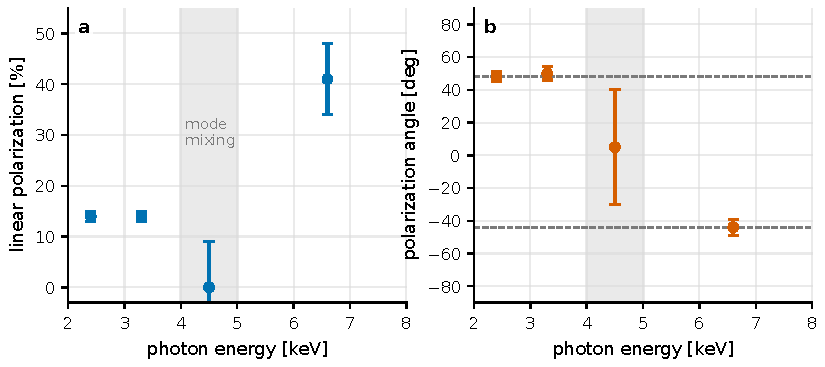
\includegraphics[width=0.92\linewidth]{figures/generated/chapter_11/ch11_birefringence_energy.pdf}
\caption{IXPE 对磁星 4U 0142+61 的结果可以看成两个偏振正常模在能量上的切换。低能 \(2-4\,\mathrm{keV}\) 偏振度约 \(14\%\)，高能 \(5.5-8\,\mathrm{keV}\) 升到约 \(41\%\)，而 \(4-5\,\mathrm{keV}\) 附近偏振度接近最低可探测偏振，偏振角发生约 \(90^\circ\) 翻转。}
\label{fig:e18-biref}
\end{figure}

把这一节收束到本书的大主线上。上面每一步——测 \(\eta_i\)、累加 Stokes、算 \(p\) 与 \(\psi\)、按相位和能量分箱——本质都是在\textbf{偏振通道上做强度/计数统计}。它和第 \ref{chap:e08} 章的 \(g^{(2)}\)、第 \ref{chap:e10} 章的强度干涉是同一族工具：只不过把"两台望远镜"或"两个时刻"换成了"两个偏振基"。第 \ref{chap:e22} 章会把这条"偏振量子通道"正式展开，讨论它在暗物质、轴子等新物理搜寻里的用法；这里的磁星双折射，就是这条通道在强场天体上最干净的一个练兵场。


\section{表面与大气辐射：热斑光变怎样反推中子星半径}
\label{sec:e18-hotspot}

最后回到"分辨不了怎么办"的老问题，但换到中子星上，答案格外漂亮。中子星半径量不到角直径（第 \ref{sec:e18-angsize} 节说过它比白矮星还小），可它偏偏能被测到 \(\sim1\,\mathrm{km}\) 的精度——靠的不是空间分辨，而是\emph{光变形状 + 能谱 + 广义相对论}。核心量是紧致度（compactness）：

\begin{equation}
  u=\frac{2GM}{Rc^2}
  \simeq 0.345
  \left(\frac{M}{1.4\,M_\odot}\right)
  \left(\frac{12\,\mathrm{km}}{R}\right).
  \label{eq:e18-compact}
\end{equation}
\begin{formulaexplain}
\(u\)：紧致度，等于史瓦西半径 \(2GM/c^2\) 与真实半径 \(R\) 之比（无量纲）。\(u\) 越大，引力对光线的弯曲越强，热斑光变的振幅越容易被抹平。
\end{formulaexplain}

物理图像：中子星表面常有一两块比周围热的斑（磁极附近的热斑，hot spot）。星一转，热斑扫过视线，我们看到脉动。可中子星的引力强到能把光线\emph{掰弯}——本来转到背面、该看不见的热斑，发出的光被引力拽回到我们视线里。紧致度越大，掰得越狠，背面的斑也能"漏"过来，于是脉冲的谷底被抬高、振幅被压平。把这个弯曲效应写成一个好用的近似，联系光子离开表面的发射角 \(\alpha\)（这里的 \(\alpha\) 是几何发射角，与前面的精细结构常数 \(\alpha_{\rm fs}\)、旋转矢量模型里的磁轴夹角 \(\alpha\) 同符不同义）和热斑相对视线的中心角 \(\psi\)（这里的 \(\psi\) 是空间角距，不是\eqref{eq:e18-pdop}、\eqref{eq:e18-rvm}里的偏振角 \(\psi\)）：

\begin{equation}
  \cos\alpha\simeq u+(1-u)\cos\psi .
  \label{eq:e18-bending}
\end{equation}
\begin{formulaexplain}
\(\alpha\)：光子离开星面时相对法线的发射角；\(\psi\)：热斑中心相对视线的角距。这个线性近似把"弯曲后一块斑还看不看得见"写成紧致度 \(u\) 的简单函数。
\end{formulaexplain}

它适用于史瓦西外部时空、慢自转到中等自转的标度估算；真正的毫秒脉冲星还要加 Doppler 增亮、光行差、时延、星体扁率和大气束射（beaming）。图~\ref{fig:e18-hotspot} 显示低紧致度时脉冲振幅大、高紧致度时谷底被抬高——半径推断正是利用这种轮廓变化 \citep{2002ApJ...566L..85B,2019AIPC.2127b0008W}。

\begin{figure}[tbp]
\centering
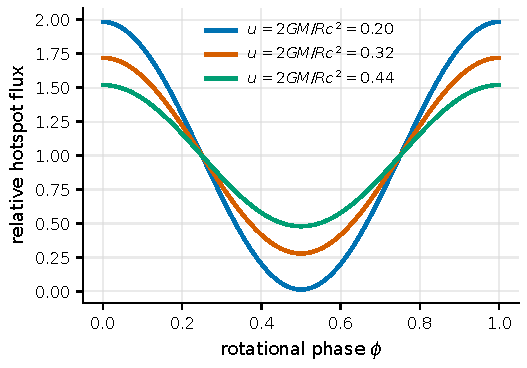
\includegraphics[width=0.78\linewidth]{figures/generated/chapter_11/ch11_hotspot_lightcurve.pdf}
\caption{热斑光变对紧致度很敏感。低紧致度时，斑点转到背面后贡献迅速消失，脉冲振幅大；高紧致度时，引力光弯曲让更大范围的表面可见，光变谷底被抬高。半径推断利用这种轮廓变化，并与质量、倾角、热斑位置和大气束射一起拟合。}
\label{fig:e18-hotspot}
\end{figure}

怎么把这套物理变成对 \(M,R\) 的测量？关键是意识到：我们手里只有一张\emph{事件表}——每个 X 射线光子带一个能量和一个自转相位。把天体模型（热斑几何 + 大气 + 引力弯曲）正向算成"每个能道、每个相位 bin 里该有多少光子"，再和实测比。第 \(j\) 个能道、第 \(k\) 个相位 bin 的期望计数是

\begin{equation}
  \lambda_{jk}(\Theta)=
  T\int dE\,R_j(E)\,
  \left[F_E(\phi_k;\Theta)+B_E\right].
  \label{eq:e18-lambda}
\end{equation}
\begin{formulaexplain}
\(\lambda_{jk}\)：能道 \(j\)、相位 bin \(k\) 的期望计数；\(T\)：曝光时间；\(R_j(E)\)：仪器响应（有效面积 + 能量重分布）；\(F_E\)：热斑模型通量；\(B_E\)：背景。\(\Theta\) 装着 \(M,R\)、距离、倾角、热斑位置等全部参数。它把天体模型翻成探测器里的预期事件数。
\end{formulaexplain}

参数向量 \(\Theta\) 里塞了 \(M,R\)、距离、观测者倾角、热斑经纬度、热斑角半径、温度和大气参数——一整套。实测计数当然不会正好等于 \(\lambda_{jk}\)，它服从泊松统计（第 \ref{chap:e03} 章）：给定期望 \(\lambda\)，观测到 \(N\) 个的概率是 \(e^{-\lambda}\lambda^N/N!\)。把所有能道、相位 bin 的概率乘起来取对数，就是泊松对数似然：

\begin{equation}
  \ln\mathcal{L}(\Theta)=
  \sum_{j,k}\left[
  N_{jk}\ln\lambda_{jk}(\Theta)-\lambda_{jk}(\Theta)-\ln(N_{jk}!)
  \right].
  \label{eq:e18-lnl}
\end{equation}
\begin{formulaexplain}
\(\ln\mathcal{L}\)：泊松对数似然；\(N_{jk}\)：实测计数。把 \(e^{-\lambda}\lambda^N/N!\) 对所有 \((j,k)\) 连乘再取对数就得到它。求半径就是找一组 \(\Theta\)，让所有 \(\lambda_{jk}\) 最贴近事件表。
\end{formulaexplain}

推导只需一步：\(\ln\prod_{jk}\dfrac{e^{-\lambda_{jk}}\lambda_{jk}^{N_{jk}}}{N_{jk}!}=\sum_{jk}\big(-\lambda_{jk}+N_{jk}\ln\lambda_{jk}-\ln N_{jk}!\big)\)。最后一项 \(\ln N_{jk}!\) 不含参数，拟合时是常数、可丢。剩下的就是要\emph{最大化}的目标——这正是第 \ref{chap:e13} 章事件表建模的通用范式，只不过这里的"天体模型"里塞进了引力弯曲和强磁场大气。NICER 对 PSR J0030+0451 和 PSR J0740+6620 的半径测量就是这么做的：J0740 的分析把 NICER 事件表、XMM-Newton 的成像光谱背景、以及射电计时给出的质量和距离先验联合起来，Riley 等得到 \(R=12.39^{+1.30}_{-0.98}\,\mathrm{km}\)、\(M=2.072^{+0.067}_{-0.066}\,M_\odot\)，Miller 等给出方法不同但相容的约束；J0030 的两套独立分析还显示热斑几何可能带复杂的多极磁场结构 \citep{2019ApJ...887L..21R,2019ApJ...887L..24M,2021ApJ...918L..27R,2021ApJ...918L..28M}。请体会这件事的分量：我们没有分辨一个 \(12\,\mathrm{km}\) 的球面（那需要纳角秒级分辨），却把它的半径量到了公里级——纯靠时间、能量和引力光学，把空间信息"折"进了事件表。


\section{本章要点}
\label{sec:e18-summary}

\begin{itemize}
\item \textbf{致密天体靠量子简并撑着，也因此"个头极小"。} 白矮星靠电子简并压（\eqref{eq:e18-pnr}、\eqref{eq:e18-per}）顶住引力，呈"越重越小"的质量–半径关系；但角直径只有微角秒（\eqref{eq:e18-theta}），中子星更小，单口径成像无望——这正把接力棒交给强度干涉（第 \ref{chap:e10} 章）和时间/偏振通道。
\item \textbf{磁场把几何写进相位和偏振。} 磁白矮星的磁层半径与共转半径之比（\eqref{eq:e18-rm}、\eqref{eq:e18-rco}）决定吸积流形态，回旋辐射带来可挑选的偏振信号；中子星的光柱、偶极磁场和自转能损失（\eqref{eq:e18-rlc}–\eqref{eq:e18-edot}）把磁层切成相位坐标，靠相位折叠（\eqref{eq:e18-fold}）读出。
\item \textbf{真空双折射是强场 QED 在偏振上的印记。} 磁星表面 \(B\) 逼近甚至超过临界场 \(B_Q\)（\eqref{eq:e18-bq}），真空变成双折射介质（\eqref{eq:e18-dn}），把星面各处的偏振"梳"齐、抬高净偏振度；4U 0142+61 的能量依赖偏振度和 \(90^\circ\) 偏振角翻转就是这类印记，但需能量、相位、多源交叉验证。
\item \textbf{偏振测量本质是"在偏振基上数光子"。} Stokes 累加（\eqref{eq:e18-stokes}）、偏振度与偏振角（\eqref{eq:e18-pdop}）、旋转矢量模型（\eqref{eq:e18-rvm}）与前面的 \(g^{(2)}\) 同宗同源，是第 \ref{chap:e22} 章"偏振量子通道"的直接前身。
\item \textbf{分辨不了，就把空间信息折进事件表。} 中子星半径靠热斑光变 + 能谱 + 引力弯曲（\eqref{eq:e18-compact}–\eqref{eq:e18-bending}），用泊松似然事件表建模（\eqref{eq:e18-lambda}、\eqref{eq:e18-lnl}）反推，NICER 已把 \(12\,\mathrm{km}\) 的中子星量到公里级。
\end{itemize}

\noindent\textbf{想一想。}
（1）为什么白矮星"越重越小"，而普通主序星"越重越大"？从简并压指数 \(5/3\to4/3\) 的软化去想。
（2）如果真空双折射\emph{不存在}，磁星的净偏振度会偏高还是偏低？为什么"一个高偏振度"能当作双折射的间接证据？
（3）中子星半径只有 \(12\,\mathrm{km}\)、角直径远小于任何望远镜的分辨极限，我们却测得出它的半径——被测量的"信息"到底藏在观测数据的哪个维度里？

\chapter{黑洞、吸积盘与 photon ring}
\label{chap:e19}

\begin{chapteropening}
黑洞没有可以反光的固体表面，我们从来没有"看见"过黑洞本身。我们看见的，是它周围被烧得发亮的气体，以及被它极端引力反复弯折的光路。想象一支火把绕着一口深不见底的井转圈：火焰本身是吸积盘的辐射，而井口那一圈幽暗轮廓，是光线在坠入之前最后绕行留下的边界——这就是黑洞阴影（black hole shadow）与它外缘那道细亮的 photon ring（光子环）。本章要把这幅画面讲清楚：吸积盘为什么会发光、发多亮、颜色怎么排布；强引力透镜如何把远处的光弯成一圈；这圈光在天空上有多大、为什么恰好落在 EHT 甚长基线阵列能分辨的门槛上；photon ring 内部为什么藏着一层层自相似的子环；最后，把前两部分学到的相干与干涉工具（\ref{chap:e08}、\ref{chap:e10}、\ref{chap:e11}）接上来，看看长基线和 \(|V|^2\) 的环状振荡在原理上还能为黑洞边缘补充什么。
\end{chapteropening}

\section{黑洞的尺度怎样定下所有坐标}
\label{sec:e19-scales}

在讨论任何具体现象之前，先要有一把尺子。黑洞问题最省事的地方，是它只有一个真正的主导参数：质量 \(M\)。一旦给定 \(M\)，长度、时间、天空角尺度就全部被锁定，剩下的物理都可以用无量纲的比值来谈。我们把这三把标尺写下来：
\begin{equation}
  r_g=\frac{GM}{c^2},\qquad
  t_g=\frac{GM}{c^3}=\frac{r_g}{c},\qquad
  \theta_g=\frac{r_g}{D}.
  \label{eq:e19-scales}
\end{equation}
\begin{formulaexplain}
\(r_g\) 是引力半径（长度），\(t_g\) 是光走过一个 \(r_g\) 的时间，\(\theta_g\) 是把 \(r_g\) 放到距离 \(D\) 处看到的角尺度。三者都正比于质量。
\end{formulaexplain}
这里 \(r_g\) 称为引力半径（gravitational radius），量纲是长度，常用 km 或 cm；它大约是史瓦西半径的一半（\(r_s=2r_g\)）。\(t_g\) 是把 \(r_g\) 除以光速得到的光行时，量纲是时间；它是黑洞附近一切动力学过程的"最快节拍"。\(D\) 是我们到黑洞的距离，\(\theta_g=r_g/D\) 是把这把长度尺子投影到天球上得到的角尺度，量纲是弧度，但天文上更常用微角秒（\(\mu{\rm as}\)，即 \(10^{-6}\) 角秒）。

先把最有用的数字算出来。在 CGS 单位下 \(G=6.674\times10^{-8}\,{\rm cm^3\,g^{-1}\,s^{-2}}\)，太阳质量 \(M_\odot=1.989\times10^{33}\,{\rm g}\)，于是 \(GM_\odot=1.327\times10^{26}\,{\rm cm^3\,s^{-2}}\)。代入 \(r_g\)：
\[
  r_g(M_\odot)=\frac{1.327\times10^{26}}{(2.998\times10^{10})^2}\,{\rm cm}
  =1.477\times10^{5}\,{\rm cm}=1.477\,{\rm km},
\]
再除以光速得到光行时：
\[
  t_g(M_\odot)=\frac{r_g}{c}=\frac{1.477\times10^{5}\,{\rm cm}}{2.998\times10^{10}\,{\rm cm\,s^{-1}}}
  =4.93\times10^{-6}\,{\rm s}=4.93\,\mu{\rm s}.
\]
把这两个"每太阳质量"的基准写成标度式，方便随手换算：
\begin{equation}
  r_g=1.477\,{\rm km}\left(\frac{M}{M_\odot}\right),\qquad
  t_g=4.93\,\mu{\rm s}\left(\frac{M}{M_\odot}\right).
  \label{eq:e19-scalenum}
\end{equation}
\begin{formulaexplain}
把质量以太阳质量为单位代进去，就直接读出引力半径（公里）和光行时（微秒）。同一套无量纲吸积过程，因质量不同会被拉到完全不同的时间尺度。
\end{formulaexplain}

这一步的物理意义值得停下来体会。取两个真实目标。银河系中心的 Sgr~A* 质量约 \(M\simeq4\times10^6\,M_\odot\)，所以 \(t_g\simeq4.93\,\mu{\rm s}\times4\times10^6\simeq20\,{\rm s}\)：靠近最内稳定圆轨道（ISCO）的物质，其结构变化只需几分钟就能显现。相比之下 M87* 的质量 \(M=(6.5\pm0.7)\times10^9\,M_\odot\)，\(t_g\simeq4.93\,\mu{\rm s}\times6.5\times10^9\simeq3.2\times10^4\,{\rm s}\simeq9\,{\rm h}\)：同样的无量纲过程会被拉长到小时甚至天的量级。于是 Sgr~A* 会在一次 VLBI 观测夜里"抖动"，而 M87* 近乎静止——这不是两种物理，而是同一种物理套在相差约 \(10^3\) 的质量上 \citep{2019ApJ...875L...1E,2019ApJ...875L...6E,2022ApJ...930L..12E}。

角尺度更有戏剧性。取常用距离，Sgr~A* 约 \(D\simeq8\,{\rm kpc}\)，M87* 约 \(D\simeq16.8\,{\rm Mpc}\)。这里要小心：\(\theta_g=r_g/D\) 只有在分子分母同单位时才是弧度，所以先把距离化成 cm。用 \(1\,{\rm kpc}=3.086\times10^{21}\,{\rm cm}\)，Sgr~A* 的 \(D=8\,{\rm kpc}=2.47\times10^{22}\,{\rm cm}\)，而它的引力半径 \(r_g=1.477\,{\rm km}\times4\times10^6=5.91\times10^{11}\,{\rm cm}\)。先算出以弧度计的角尺度，再乘 \(1\,{\rm rad}=2.063\times10^{11}\,\mu{\rm as}\) 换成微角秒：
\[
  \theta_g^{\rm SgrA*}=\frac{r_g}{D}
  =\frac{5.91\times10^{11}\,{\rm cm}}{2.47\times10^{22}\,{\rm cm}}
  =2.39\times10^{-11}\,{\rm rad}
  \times 2.063\times10^{11}\,\frac{\mu{\rm as}}{\rm rad}
  \approx 4.9\,\mu{\rm as}.
\]
M87* 同法：\(r_g=1.477\,{\rm km}\times6.5\times10^9=9.6\times10^{14}\,{\rm cm}\)，\(D=16.8\,{\rm Mpc}=5.18\times10^{25}\,{\rm cm}\)，得 \(\theta_g^{\rm M87*}=1.85\times10^{-11}\,{\rm rad}\approx3.8\,\mu{\rm as}\)。质量相差 \(10^3\)、距离也相差约 \(10^3\)，两个 \(\theta_g\) 便都落在几微角秒。把 \(\theta_g\) 乘上下一节要讲的阴影系数 \(\kappa\simeq10.4\)，就得到几十微角秒的阴影——这正是 EHT 的观测门槛。图~\ref{fig:e19-scales} 把这层"质量线性控制一切"的关系画了出来。

\begin{figure}[tbp]
\centering
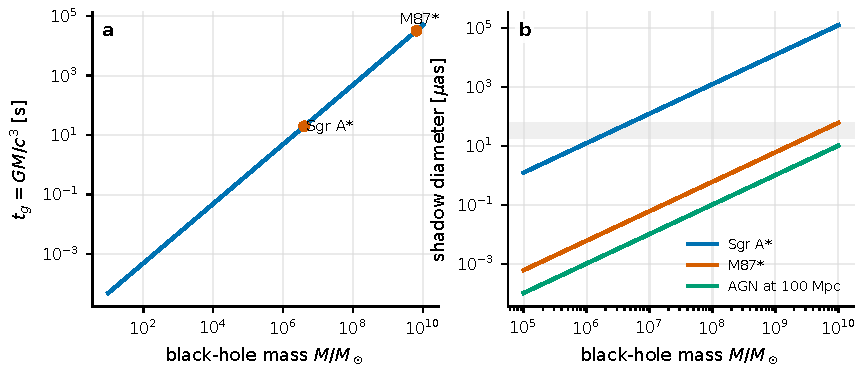
\includegraphics[width=0.94\linewidth]{figures/generated/chapter_12/ch12_black_hole_scales.pdf}
\caption{黑洞的时间尺度和角尺度都由质量线性控制。Sgr~A* 和 M87* 的质量相差约 \(10^3\)，但距离也相差约 \(10^3\)，所以二者的阴影角直径都在几十微角秒；时间尺度却完全不同：Sgr~A* 可以在一次 VLBI 扫描内改变，M87* 的结构更接近静态。}
\label{fig:e19-scales}
\end{figure}

有了尺子，就可以把黑洞观测的"事件表坐标"写全。前几章我们把一次光子探测记成到达时间和频率；到了黑洞成像，坐标要扩展为
\[
  (t_i,\ \nu_i,\ \bm{b}_i,\ \eta_i,\ w_i),
\]
其中 \(t_i\) 是到达时间，\(\nu_i\) 是频率或能道，\(\bm{b}_i\) 是投影基线（决定测到哪个空间频率），\(\eta_i\) 是偏振通道，\(w_i\) 是权重。EHT 的复可见度、GRAVITY 的差分相位、光学监测的光变，都可以看成这张事件表的不同投影。关键在于：投影之前尽量保留时间和偏振，才能把吸积流变化、喷流扰动和强引力多路径分开估计。这条思路和 \ref{chap:e11} 里"从可见度到成像"是同一套语言，只是现在测量对象换成了强引力弯折过的光。

\section{吸积盘怎样产生连续谱和随机光变}
\label{sec:e19-disk}

黑洞不发光，发光的是落向它的气体。气体带着角动量，无法直接掉进去，只能盘旋着一圈圈向内、彼此摩擦、把引力势能磨成热，最后辐射出去——这就是吸积盘（accretion disk）。标准薄盘模型给出单位面积的辐射通量：
\begin{equation}
  F(R)=\frac{3GM\dot M}{8\pi R^3}
  \left[1-\left(\frac{R_{\rm in}}{R}\right)^{1/2}\right],
  \label{eq:e19-flux}
\end{equation}
\begin{formulaexplain}
\(F(R)\) 是盘上半径 \(R\) 处单位面积向外辐射的功率，\(\dot M\) 是吸积率，\(R_{\rm in}\) 是内边界。方括号让通量在内边界处归零。
\end{formulaexplain}
逐个符号看：\(R\) 是盘半径（cm），\(\dot M\) 是吸积率（\({\rm g\,s^{-1}}\)），\(R_{\rm in}\) 是盘的内边界，通常取几倍 \(r_g\)（对无自旋黑洞 ISCO 在 \(6r_g\)）。方括号 \([\,1-(R_{\rm in}/R)^{1/2}\,]\) 保证物质在内边界处不再有净力矩、通量趋零；一旦 \(R\gg R_{\rm in}\)，方括号趋近 1，主导行为就是 \(F\propto R^{-3}\)。

若盘在局部近似黑体，把通量换成温度：
\begin{equation}
  T(R)=\left[\frac{F(R)}{\sigma_{\rm SB}}\right]^{1/4},
  \label{eq:e19-temp}
\end{equation}
\begin{formulaexplain}
\(T(R)\) 是盘在半径 \(R\) 的局部有效温度，\(\sigma_{\rm SB}\) 是 Stefan--Boltzmann 常数。薄盘光谱的颜色，是不同半径黑体温度叠加出来的。
\end{formulaexplain}
在远离内边界处 \(F\propto R^{-3}\)，代入并注意四次方根：
\[
  T(R)\propto \big(R^{-3}\big)^{1/4}=R^{-3/4}
  \quad\Longrightarrow\quad
  T(R)\propto (M\dot M)^{1/4}\,R^{-3/4}.
\]
这就是薄盘最著名的温度律：越往里越热，颜色越蓝。现在问一个观测者会问的问题——某个波长 \(\lambda\) 主要来自哪个半径？黑体在波长 \(\lambda\) 处最亮时满足 Wien 关系 \(k_{\rm B}T\sim hc/\lambda\)，也就是 \(T\propto1/\lambda\)。把这个条件塞进温度律：
\[
  \frac{1}{\lambda}\propto (M\dot M)^{1/4}R_\lambda^{-3/4}
  \;\Longrightarrow\;
  R_\lambda^{3/4}\propto (M\dot M)^{1/4}\lambda
  \;\Longrightarrow\;
  R_\lambda\propto (M\dot M)^{1/3}\lambda^{4/3}.
\]
写成标度式：
\begin{equation}
  R_\lambda \propto (M\dot M)^{1/3}\,\lambda^{4/3}.
  \label{eq:e19-Rlambda}
\end{equation}
\begin{formulaexplain}
\(R_\lambda\) 是波长 \(\lambda\) 附近主要发光的盘半径。波长越长来自越外层；质量和吸积率越大，同一颜色的发光环也越大。
\end{formulaexplain}
这条 \(R_\lambda\propto\lambda^{4/3}\) 是可以被观测检验的"指纹"。对 \(M\sim10^8\,M_\odot\)、爱丁顿比 \(L/L_{\rm Edd}\sim0.1\) 的类星体，光学到近紫外连续谱大致来自 \(0.1\)–\(10\) 光日（light-day）量级的半径。有意思的是，微透镜和多波段延迟测量经常给出比最简薄盘更大的光学盘，这正是非均匀盘（inhomogeneous disk）和再处理（reprocessing）模型被反复讨论的原因 \citep{1973A&A....24..337S,2006ApJ...642...87P,2011ApJ...727L..24D}。图~\ref{fig:e19-disk} 左侧的橙色区域就示意了这种"实测光学盘偏大"的情形。

\begin{figure}[tbp]
\centering
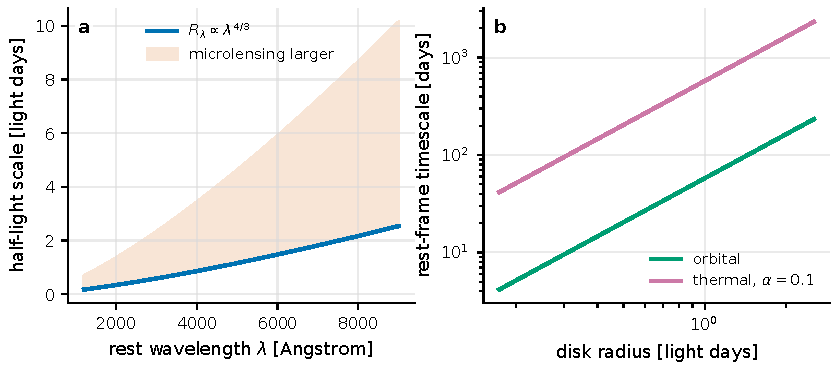
\includegraphics[width=0.94\linewidth]{figures/generated/chapter_12/ch12_accretion_disk_radii.pdf}
\caption{薄盘标度给出 \(R_\lambda\propto\lambda^{4/3}\)。左图橙色区域表示微透镜和部分连续谱延迟常暗示的更大光学发光面积；右图比较同一半径上的轨道时间和热时间，若 \(\alpha\simeq0.1\)，热时间约为轨道时间的十倍。}
\label{fig:e19-disk}
\end{figure}

发光是一幅静态图，但吸积盘还在不停"闪烁"。要理解光变的时间尺度，先估计盘上一个半径处的两把时钟：
\begin{equation}
  t_{\rm orb}=2\pi\left(\frac{R^3}{GM}\right)^{1/2},\qquad
  t_{\rm th}\simeq\frac{t_{\rm orb}}{\alpha}.
  \label{eq:e19-times}
\end{equation}
\begin{formulaexplain}
\(t_{\rm orb}\) 是开普勒轨道周期，\(t_{\rm th}\) 是热时间（局部储能被辐射改写所需的时间），\(\alpha\) 是粘滞参数。扰动落在哪把时钟上，决定光变能多快响应。
\end{formulaexplain}
\(t_{\rm orb}\) 就是把开普勒第三定律 \(\Omega^2=GM/R^3\) 取周期 \(2\pi/\Omega\) 得到的轨道时间；\(t_{\rm th}\) 是热时间，即局部储热被辐射重新分配所需的时间。\(\alpha\) 是 Shakura--Sunyaev 粘滞参数（无量纲），常取 \(0.01\)–\(0.3\)。因为 \(\alpha<1\)，热时间总比轨道时间长，图~\ref{fig:e19-disk} 右侧取 \(\alpha\simeq0.1\) 时二者相差约十倍。对 AGN 光学盘，\(t_{\rm orb}\) 可以是几十天到几年，\(t_{\rm th}\) 更长——这就是为什么类星体的光学光变以"月到年"为节拍。

大样本光学光变常用阻尼随机游走（damped random walk, DRW）来描述，它的自协方差和功率谱是一对：
\begin{equation}
  C(\tau)=\sigma^2\exp\!\left(-\frac{|\tau|}{\tau_d}\right),
  \qquad
  P(f)\propto\frac{1}{1+(2\pi f\tau_d)^2}.
  \label{eq:e19-drw}
\end{equation}
\begin{formulaexplain}
\(C(\tau)\) 是光变的自协方差，\(\tau_d\) 是阻尼（记忆）时间，\(P(f)\) 是功率谱。这个模型把随机光变写成一个"会慢慢忘掉自己"的相关过程。
\end{formulaexplain}
先点名符号：\(\sigma^2\) 是光变的方差（长时间尺度上亮度起伏振幅的平方），因此 \(\sigma\) 与被测的亮度（或流量）同量纲，量纲就是流量/星等的量纲；\(\tau\) 是时间延迟，\(f\) 是频率。这里两式互为傅里叶变换：指数型自协方差的谱是洛伦兹型（\ref{chap:e02} 里我们正是用这一对关系把相关时间和带宽联系起来的）。物理图像很直白：\(\tau_d\) 是盘"记得自己上一刻多亮"的时间；比 \(\tau_d\) 短的时标上光变高度相关，比它长就渐渐失忆，功率谱在 \(f\gtrsim1/2\pi\tau_d\) 处转入 \(f^{-2}\) 衰减。观测上 \(\tau_d\) 与黑洞质量相关，超大质量黑洞常为数十到数百天（静止系）\citep{1993ApJ...406..420M,2021Sci...373..789B,2016Natur.534...75M}。图~\ref{fig:e19-var} 对比了短、长两种 \(\tau_d\) 的记忆行为。

\begin{figure}[tbp]
\centering
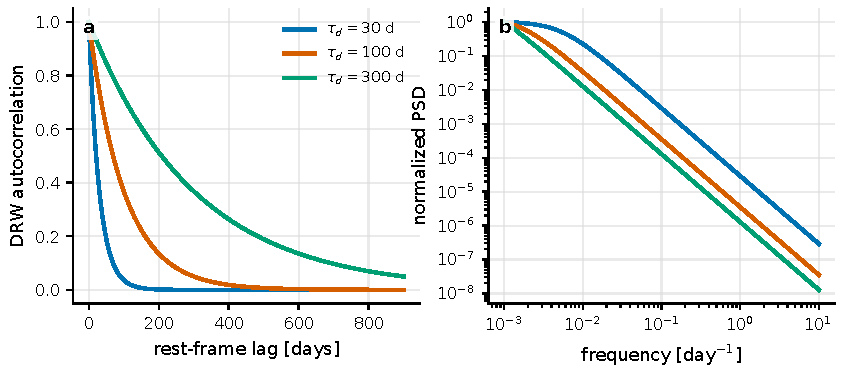
\includegraphics[width=0.94\linewidth]{figures/generated/chapter_12/ch12_variability_autocorrelation.pdf}
\caption{阻尼随机游走把随机光变写成一个相关时间。短 \(\tau_d\) 的光变很快失去记忆，功率谱较早转入 \(f^{-2}\) 衰减；长 \(\tau_d\) 的盘在更长时间上保持相关，低频平台延伸得更远。}
\label{fig:e19-var}
\end{figure}

这里要给对光子统计感兴趣的读者一句诚实的提醒。前几章的 \(g^{(2)}\) bunching（\ref{chap:e08}）是单模热光的量子指纹；但一个 \(10^8\,M_\odot\) 的 AGN 光学连续谱来自海量彼此独立的湍流小区和多个热时间的叠加，属于极端多模。多模会把每一模的 bunching 平均掉，测到的 \(g^{(2)}\) 几乎压到 1。所以吸积盘上更现实的可测量，不是原始 bunching，而是在相位或颜色条件下的"过量相关"——例如比较 flare 前后 \(g^{(2)}(\tau)\) 宽度的变化，或把偏振通道分开来读湍流胞元的寿命。平均亮度主要给出光子率和归一化；能不能真正测到相关，还受相干时间、采样窗口和经典涨落可否建模的联合约束。

\section{强引力透镜与 photon ring 的几何起源}
\label{sec:e19-geometry}

现在走到本章的核心画面：那圈亮环是怎么来的。关键在于，黑洞附近的光不走直线。想象你站在很远处，向黑洞方向平行射出许多光线，每条光线用它的碰撞参数（impact parameter）\(b\) 标记——\(b\) 就是"如果没有引力，这条光线会从黑洞旁多远处擦过"。引力会把光线往里掰：
\begin{itemize}
\item \(b\) 很大时，光线只被轻微偏折，径直飞过；
\item \(b\) 逐渐减小，偏折越来越狠，光线开始绕黑洞转小半圈、一圈、几圈；
\item 存在一个临界值 \(b_c\)：恰好等于它时，光线会无限逼近某个圆轨道盘旋不去；小于它，光线一头栽进黑洞，再也出不来。
\end{itemize}
那个让光"能绕圈"的圆轨道，叫光子球（photon sphere）。对无自旋（史瓦西）黑洞，光子球半径和临界碰撞参数是标准的广义相对论结果：
\begin{equation}
  r_{\rm ph}=3\,\frac{GM}{c^2}=3\,r_g,\qquad
  b_c=3\sqrt{3}\,\frac{GM}{c^2}=3\sqrt{3}\,r_g\approx5.196\,r_g.
  \label{eq:e19-photonsphere}
\end{equation}
\begin{formulaexplain}
\(r_{\rm ph}\) 是光子能做圆周运动的半径，\(b_c\) 是能逃逸与被吞没之间的临界碰撞参数。它们只依赖 \(r_g\)，也就是只依赖质量。
\end{formulaexplain}
这两个数怎么理解？\(r_{\rm ph}=3r_g\) 说明光子球坐落在史瓦西半径（\(2r_g\)）之外一点，是"光还能勉强绕圈但极不稳定"的地方；任何微小扰动都会让绕行的光要么向内坠落、要么向外逃逸。\(b_c=3\sqrt3\,r_g\) 则是天球上的分界线：来自背景、碰撞参数 \(b<b_c\) 的光都进了黑洞，于是我们看到一块暗斑；\(b\) 稍大于 \(b_c\) 的光会绕行若干圈后逃出，叠在暗斑外缘，堆成一道细亮的环。这道环就是 photon ring。

暗斑的大小是可以直接算的。观测者看到的阴影半径正是临界碰撞参数投影到天空的角度，阴影角直径为
\begin{equation}
  d_{\rm sh}=\frac{2b_c}{D}=6\sqrt{3}\,\frac{r_g}{D}=6\sqrt{3}\,\theta_g\simeq10.4\,\theta_g,
  \label{eq:e19-shadow}
\end{equation}
\begin{formulaexplain}
\(d_{\rm sh}\) 是黑洞阴影的角直径，等于 \(2b_c\) 除以距离。系数 \(6\sqrt3\approx10.4\) 是纯几何常数，把引力半径角尺度放大约十倍。
\end{formulaexplain}
这一步把上一节埋下的系数 \(\kappa\simeq10.4\) 兑现了：它不是拟合出来的经验数，而是 \(6\sqrt3\) 这个几何常数。对旋转（Kerr）黑洞，自旋和倾角会让阴影略微不圆、系数在百分之几到十来个百分点内浮动，但量级不变，所以我们仍可放心地用 \(d_{\rm sh}\simeq10.4\,\theta_g\) 做估计。

代入上一节的角尺度就得到可观测的环。M87* 的 \(\theta_g\simeq3.8\,\mu{\rm as}\)，预言 \(d_{\rm sh}\simeq10.4\times3.8\simeq40\,\mu{\rm as}\)；EHT 在 \(1.3\,{\rm mm}\) 实测到的非对称环直径为 \(42\pm3\,\mu{\rm as}\)，环中心亮度被压低超过十倍——正是阴影。Sgr~A* 的 \(\theta_g\simeq4.9\,\mu{\rm as}\)，预言 \(d_{\rm sh}\simeq51\,\mu{\rm as}\)，实测厚环直径 \(51.8\pm2.3\,\mu{\rm as}\)，只是源在观测夜内有明显的分钟到小时级变化 \citep{2019ApJ...875L...4E,2019ApJ...875L...5E,2022ApJ...930L..14E,2022ApJ...930L..15E}。一个纯几何常数 \(6\sqrt3\) 乘上一把由质量定的尺子，就把广义相对论预言压到了两位有效数字，与观测吻合——这是本章最值得记住的画面。

要提醒的是：EHT 看到的亮环并不是数学上无限薄的 photon ring。它是几样东西叠在一起：吸积流本身的直接辐射、绕行半圈左右的"一次透镜像"，以及绕行多圈的高阶 photon subring（光子子环）。吸积流的厚度、光深、湍流和时间平均会把强引力的窄结构涂宽。下一节就来看这层层嵌套的子环。

\section{photon ring 的自相似子环结构}
\label{sec:e19-subring}

photon ring 最迷人的性质，是它内部藏着一套自相似的分层结构。回到几何图像：碰撞参数越接近临界值 \(b_c\)，光在逃逸前绕黑洞的圈数越多。我们按"绕行半圈数"给这些像编号 \(n=0,1,2,\dots\)：\(n=0\) 是几乎不绕的直接像，\(n=1\) 是绕约半圈打到另一侧的一次透镜像，\(n\) 越大绕得越多，也越贴近那条临界曲线。每多绕一圈，对应的亮环就更窄、更暗，并且更逼近同一个极限半径。把第 \(n\) 个子环的角宽度和通量写成标度形式：
\begin{equation}
  w_n\simeq w_0\,e^{-\gamma n},\qquad
  F_n\simeq F_0\,e^{-\beta n}.
  \label{eq:e19-subring}
\end{equation}
\begin{formulaexplain}
\(w_n\) 和 \(F_n\) 是第 \(n\) 个 photon subring 的角宽度和通量。两者都随 \(n\) 指数衰减：子环一层层变窄、变暗，并向临界曲线收拢。
\end{formulaexplain}
这里 \(w_0,F_0\) 是最外层（低阶）结构的宽度和通量标度，\(\gamma\) 与 \(\beta\) 是控制"每绕一圈缩小多少"的衰减指数（无量纲）。指数 \(\gamma\) 由光子球轨道的不稳定性决定——正是那条极不稳定的圆轨道的 Lyapunov 指数，刻画相邻光线在绕行中彼此分离的速率；\(\beta\) 还额外取决于沿途的发射与吸收。物理上，\(w_n\sim e^{-\gamma n}\) 意味着子环以近乎固定的比例逐层变窄，形成一套"环套环"的自相似梯子；而 \(F_n\sim e^{-\beta n}\) 意味着高阶子环虽然位置越来越普适（几乎只由 Kerr 度规决定、与吸积流细节无关），通量却越来越小，越来越难测。

这套自相似结构的意义在于它的普适性：低阶像的形状受吸积流的脏细节污染，但足够高阶的子环几乎只记得时空几何本身。理论对史瓦西黑洞给出很干净的结果——每往高一阶，子环的位置、宽度按大约固定的因子收缩、通量按大约固定的因子变暗，收拢到 \(b_c\) 对应的临界曲线上 \citep{2019PhRvD.100b4018G,2020PhRvD.102l4004G,2020SciA....6.1310J}。Gralla 等强调：在总通量里，高阶 photon ring 往往只占很小一份，直接从图像上分离它们非常困难。这就把问题推向了下一节——如果图像域看不清，能不能换到可见度域去看。

\section{EHT 甚长基线成像与可见度里的环状振荡}
\label{sec:e19-visibility}

要分辨几十微角秒的环，光靠单口径望远镜是没戏的：衍射极限 \(\theta\sim\lambda/D_{\rm tel}\)，在 \(1.3\,{\rm mm}\) 要达到 \(20\,\mu{\rm as}\) 需要口径
\[
  D_{\rm tel}\sim\frac{\lambda}{\theta}
  =\frac{1.3\times10^{-3}\,{\rm m}}{20\,\mu{\rm as}}
  =\frac{1.3\times10^{-3}}{20\times4.848\times10^{-12}\,{\rm rad}}
  \approx1.3\times10^{7}\,{\rm m},
\]
也就是地球直径的量级。这正是甚长基线干涉（VLBI）存在的理由：把分布在全球的望远镜连成一台"地球大小"的合成望远镜。干涉仪不直接给图像，它测的是天空亮度分布的傅里叶分量——复可见度：
\begin{equation}
  V(\bm{u})=\int I(\bm{\theta})\,
  e^{-2\pi i\,\bm{u}\cdot\bm{\theta}}\,d^2\theta,
  \qquad
  \bm{u}=\frac{\bm{B}_\perp}{\lambda}.
  \label{eq:e19-vis}
\end{equation}
\begin{formulaexplain}
\(V(\bm u)\) 是复可见度，\(I(\bm\theta)\) 是天空亮度分布，\(\bm u=\bm B_\perp/\lambda\) 是以波长为单位的投影基线（空间频率）。基线越长，看到的空间频率越高，能分辨的角结构越细。
\end{formulaexplain}
这就是 \ref{chap:e10}、\ref{chap:e11} 里 van~Cittert--Zernike 与"可见度即傅里叶分量"的老朋友，只是现在源是一圈被引力弯出来的光。一个理想化的均匀薄环，它的可见度有一个漂亮的解析形式：
\begin{equation}
  V(u)\simeq J_0(\pi d\,u),
  \label{eq:e19-bessel}
\end{equation}
\begin{formulaexplain}
\(J_0\) 是零阶贝塞尔函数，\(d\) 是环的角直径，\(u\) 是基线长度对应的空间频率。薄环的可见度随基线振荡，并在一系列基线上出现零点。
\end{formulaexplain}
为什么是贝塞尔函数？一个半径固定的细环，把它绕一圈的傅里叶积分做出来，角向积分正好给出 \(J_0\)——这与一个圆孔的衍射会出现贝塞尔型花样是同一类几何。要点是：\(J_0(x)\) 是一条振荡衰减的曲线，在 \(x=2.405,\,5.520,\dots\) 处依次穿零。于是环在可见度上留下的指纹，是一串随基线拉长而出现的\emph{零点与旁瓣}——\(|V|^2\) 呈环状振荡，而不是像一个光滑光斑那样单调下降。

把第一个零点落在哪条基线上算出来，就明白 EHT 为什么"刚好够用"。第一个零点在 \(\pi d\,u=2.405\)，即
\[
  u_{\rm null}=\frac{2.405}{\pi d}=\frac{0.765}{d}.
\]
对 M87* 的 \(d\simeq42\,\mu{\rm as}=2.04\times10^{-10}\,{\rm rad}\)：
\[
  u_{\rm null}=\frac{0.765}{2.04\times10^{-10}}\approx3.8\times10^{9}
  =3.8\,{\rm G}\lambda,
\]
换算成实际基线长度 \(B_\perp=u_{\rm null}\,\lambda=3.8\times10^9\times1.3\times10^{-3}\,{\rm m}\approx4.9\times10^{6}\,{\rm m}\)，约 \(5000\,{\rm km}\)——远小于地球直径。也就是说，地球尺度的 \(1.3\,{\rm mm}\) VLBI 恰好能越过第一个可见度谷，直接在可见度域"摸到"环状结构 \citep{2019ApJ...875L...2E,2019ApJ...875L...3E,2020SciA....6.1310J}。

真实的环不是无限薄的。若环有有限宽度 \(w\)，它相当于把理想 \(J_0\) 乘上一个宽度反比于 \(w\) 的包络：宽的结构在较短基线上就被"抹掉"，窄的结构才能在很长的基线上继续保留振荡。这一点把上一节的自相似子环和可见度域连了起来——见图~\ref{fig:e19-ring}。

\begin{figure}[tbp]
\centering
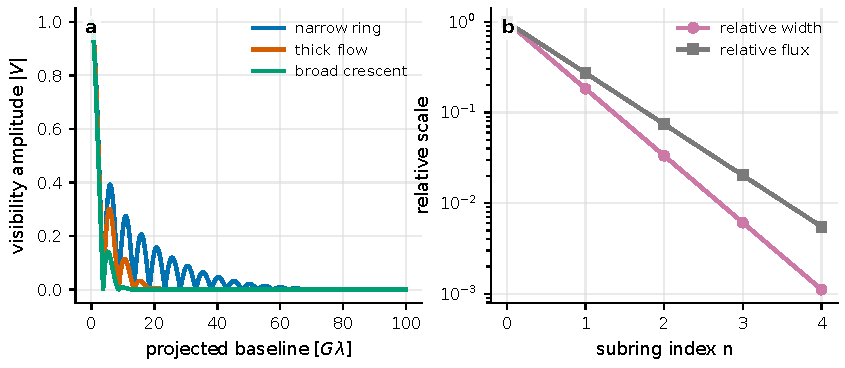
\includegraphics[width=0.94\linewidth]{figures/generated/chapter_12/ch12_photon_ring_visibility.pdf}
\caption{环状结构在长基线可见度中产生振荡。左图比较同样 \(42\,\mu{\rm as}\) 直径下不同厚度的环，窄环在更长基线上仍保留振荡；右图示意 photon subring 的宽度和通量随环绕次数下降，高阶子环通量小，但在足够长的基线上可留下普适的振荡结构。}
\label{fig:e19-ring}
\end{figure}

这就给出了一个漂亮的策略：在图像域里，宽而亮的吸积流盖过了窄而暗的高阶子环；但在可见度域里，随着基线拉长，宽吸积流的贡献先被"解析掉"（其可见度早早衰减到噪声以下），剩下的长基线信号越来越由最窄的 photon subring 主导，露出它那套几乎只由时空几何决定的普适振荡 \citep{2013ApJ...777..170J,2020SciA....6.1310J}。换句话说，够长的基线是一把梳子，能把强引力的普适结构从吸积流的脏背景里梳出来。

\section{干涉与相干方法在原理上还能补充什么}
\label{sec:e19-coherence}

把前两部分的工具接上来，看看它们在原理上能为黑洞边缘结构补充什么。核心有三条。

\textbf{第一，长基线揭示普适子环。} 如上节所述，可见度域的关键资源是基线长度 \(u=B_\perp/\lambda\)。地面 EHT 的基线以地球直径封顶，只够看到第一、第二个可见度谷；要把第 \(n\ge2\) 阶子环那越来越窄、位置越来越普适的振荡挖出来，需要把基线延伸到地球之外（空间 VLBI）或缩短波长。这不是新物理，而是把 \ref{chap:e11} 里"更长基线 = 更高空间频率 = 更细角结构"的原则推到极限：photon ring 的自相似性保证了，只要基线够长，总有一层子环在等着被分辨。

\textbf{第二，\(|V|^2\) 的环状振荡本身就是一种相干测量。} 强度干涉（\ref{chap:e10}）测的正是 \(|V|^2\)（丢掉相位），而环的 \(|V|^2\) 恰恰是一串贝塞尔零点与旁瓣——一种即便没有相位也能识别的"环状指纹"。这为亮、角尺度较大的目标提供了一条不依赖大气相位稳定、可用超长基线的原理性通道：只要能在足够长的基线上测到 \(|V|^2\) 的振荡是否守时、零点落在何处，就能约束环的直径与宽度。代价是强度干涉信号弱、要求极高的光子通量和长积分，对多数黑洞源在近期仍是原理性的而非现成可行的。

\textbf{第三，多路径会在时间结构里留下回声。} 光绕行不同圈数，路径长度不同，到达时间也不同。若第 \(n\) 圈与第 \(n+1\) 圈的平均延迟差接近光子轨道周期 \(T_\gamma\)，那么强度自相关
\begin{equation}
  C(\tau)=\big\langle\delta I(t)\,\delta I(t+\tau)\big\rangle
  \quad\text{可能在}\quad
  \tau\simeq m\,T_\gamma\ (m=1,2,\dots)
  \label{eq:e19-echo}
\end{equation}
\begin{formulaexplain}
\(C(\tau)\) 是强度涨落的自相关，\(T_\gamma\) 是光子绕黑洞一圈的周期，\(m\) 是整数。若多路径贡献可见，自相关会在这些延迟处出现微弱回声峰。
\end{formulaexplain}
附近出现微弱的峰。物理图像是：同一次闪烁的光，一部分直接到达，一部分多绕一圈后晚 \(T_\gamma\) 到达，二者在时间序列里形成"回声"。对 Sgr~A*，\(T_\gamma\) 是分钟量级，正好和吸积流本身的 flare 时标重叠，容易混淆；对 M87*，\(T_\gamma\) 是天量级，源更稳定但观测调度更难。要把这类峰真正解释成强引力多路径，必须先排除喷流激波、盘湍流、散射屏、采样窗口和校准误差——这是一个高门槛的、原理上可行但实践上苛刻的目标。偏振版本还可进一步比较 \(Q,U,V\) 各 Stokes 分量的延迟结构，EHT 对 M87* 和 Sgr~A* 的偏振成像已经展示了这类信息的价值 \citep{2021ApJ...910L..13E,2021PhRvD.104d4049G,2022PhRvD.106d3021C}。

需要给读者一个如实的边界。这些相干手段能补充的是\emph{边缘的角结构与时间结构}，不是黑洞自身的量子辐射。真正属于黑洞本身的量子过程——Hawking 辐射（\ref{chap:e16} 会从辐射机制角度再提）——其温度 \(T_H\propto1/M\) 对恒星质量黑洞已远低于 \(2.725\,{\rm K}\) 的宇宙微波背景，对 Sgr~A*、M87* 更低到 \(10^{-14}\)–\(10^{-17}\,{\rm K}\)，蒸发时标远超宇宙年龄，不在可预见望远镜的灵敏度之内 \citep{1974Natur.248...30H,1975CMaPh..43..199H}。所以对天体质量与超大质量黑洞，近期真正可操作的观测主线仍然是本章讲的这四样：吸积流、偏振、可见度、以及 photon ring 的时间与角结构。

\section{本章要点}
\label{sec:e19-summary}

\begin{itemize}
\item \textbf{一把尺子定全局。} 黑洞的长度、时间、角尺度都正比于质量：\(r_g=1.477\,{\rm km}\,(M/M_\odot)\)，\(t_g=4.93\,\mu{\rm s}\,(M/M_\odot)\)，\(\theta_g=r_g/D\)。Sgr~A* 与 M87* 质量差 \(10^3\)、距离也差 \(10^3\)，故阴影都落在几十微角秒，但时间尺度一为秒、一为小时。
\item \textbf{吸积盘的颜色与闪烁。} 薄盘温度律 \(T\propto R^{-3/4}\) 给出 \(R_\lambda\propto(M\dot M)^{1/3}\lambda^{4/3}\)：波长越长来自越外层。光变以轨道时间和热时间为节拍，可用阻尼随机游走的相关时间 \(\tau_d\) 概括。多模稀释会把原始 bunching 抹平。
\item \textbf{photon ring 的几何起源。} 光子球在 \(r_{\rm ph}=3r_g\)，临界碰撞参数 \(b_c=3\sqrt3\,r_g\)。阴影角直径 \(d_{\rm sh}=6\sqrt3\,\theta_g\simeq10.4\,\theta_g\)——系数是纯几何常数，把 \(\theta_g\) 放大约十倍，预言与 EHT 实测（M87* 约 \(42\,\mu{\rm as}\)、Sgr~A* 约 \(52\,\mu{\rm as}\)）两位有效数字吻合。
\item \textbf{自相似子环。} 高阶子环宽度 \(w_n\sim e^{-\gamma n}\)、通量 \(F_n\sim e^{-\beta n}\) 逐层收窄变暗，向临界曲线收拢；\(\gamma\) 由光子轨道的 Lyapunov 指数决定，越高阶越普适、越难测。
\item \textbf{可见度里的环状指纹。} 薄环可见度 \(V(u)\simeq J_0(\pi d u)\) 在基线上振荡穿零，第一个零点对 M87* 落在约 \(5000\,{\rm km}\) 基线——地球尺度 VLBI 刚好越得过。够长的基线能把宽吸积流解析掉，露出窄子环的普适振荡。
\item \textbf{相干方法能补什么。} 原理上有三条：更长基线揭示更高阶普适子环；\(|V|^2\) 的环状振荡是不依赖相位的相干指纹；强度自相关在 \(\tau\simeq mT_\gamma\) 处可能出现多路径回声。三者补充的是边缘结构，不是 Hawking 辐射——后者对天体黑洞远在可观测门槛之下。
\end{itemize}

\noindent\textbf{想一想。}
\begin{itemize}
\item 若把观测波长从 \(1.3\,{\rm mm}\) 缩短到 \(0.87\,{\rm mm}\)，同一条地面基线对应的空间频率 \(u=B_\perp/\lambda\) 如何变化？这对分辨 photon ring 的可见度振荡是有利还是不利？
\item 阴影系数 \(6\sqrt3\) 来自史瓦西几何。若黑洞高速自旋，你预期阴影会怎样偏离正圆？为什么本章仍能安心用 \(d_{\rm sh}\simeq10.4\,\theta_g\) 做量级估计？
\item 对 Sgr~A*，光子轨道周期 \(T_\gamma\) 是分钟量级，与吸积流 flare 时标重叠。要把强度自相关在 \(\tau\simeq mT_\gamma\) 处的弱峰归因于强引力多路径，你会设计怎样的对照来排除吸积流本身的贡献？
\end{itemize}

\chapter{爆发、瞬变与多信使量子天文学}
\label{chap:e20}

\begin{chapteropening}
到目前为止，我们大多在看"稳定"的天体：一颗恒星的角直径、一个吸积盘的相干性、一段可以慢慢积分几个小时的信号。可宇宙里还有另一半——它们不给你几个小时，只给你几秒、几毫秒，甚至几纳秒。一颗白矮星表面的热核爆炸、两颗中子星并合迸出的火球、一束扫过地球的射电闪光，都是"来了就走"的事件。它们把一整套物理过程压缩到一根很短的时间轴上，逼着我们回答同一个问题：\textbf{当信号转瞬即逝时，我们究竟应该记录什么、怎样从零星几个光子里把物理量抠出来？}

本章的主线是：先说清楚为什么面对瞬变，第 \ref{chap:e13} 章那张"事件表"（每个光子带着时间、频率、偏振标签）比一条平滑的光变曲线值钱得多；再把触发（trigger）看成一次统计推断，而不是"看到亮点就报警"；然后回到本书的老本行——瞬变源的光子统计与相干性；最后走进多信使（multi-messenger）时代，看引力波、中微子、光子这三路信使怎样靠\textbf{时间}被缝合成同一个物理事件。沿途我们会用膨胀新星、千新星、伽马暴余辉和潮汐瓦解事件当四个真实的算例。
\end{chapteropening}

\section{快变宇宙：为什么要留下每个光子的时间标签}
\label{sec:e20-fast}

先建立画面。一条\textbf{光变曲线}（light curve）是把光子按时间分箱、每箱数个数、连成的一条线。它很直观，但它做了一件不可逆的事：把"第 3.417\,922 秒到了一个 512\,nm 的光子"这种细节，抹成了"第 3.4 秒那一箱里有 217 个光子"。对一颗慢慢变亮的恒星，这没什么损失；可对瞬变源，时间结构本身就是物理。

伽马暴（gamma-ray burst，GRB）的 prompt emission 里，光变可以在\(10^{-2}\,\mathrm{s}\)的尺度上剧烈起伏；快速射电暴（fast radio burst，FRB）的主脉冲往往只有毫秒宽，内部还有亚毫秒的精细结构；脉冲星（pulsar）的每一个脉冲更是像钟摆一样按毫秒周期精确到达。这些结构一旦被粗分箱平均掉，就再也回不来了。所以第 \ref{chap:e13} 章才坚持把每个光子候选写成事件表里的一行——保留它的到达时刻 \(t\)、频率/能道、偏振通道，而不是只存一条曲线。这不是洁癖，而是因为下面这条似然只有在\textbf{未分箱}（unbinned）时才不丢信息。

把某个探测通道里光子的\textbf{瞬时到达率}记作 \(\lambda(t)\)，单位是 \(\mathrm{s^{-1}}\)。第 \ref{chap:e03} 章讲过：在极短一段时间里出现一个光子的概率正比于率乘以时长，且互不影响——这就是\textbf{非齐次泊松点过程}（inhomogeneous Poisson point process）。第 \ref{chap:e14} 章已经从"把时间切成无穷窄的小格再取 \(\Delta t\to0\)"一步步推出了它的对数似然，这里直接点名并使用这个结果：
\begin{equation}
  \ln L=\sum_{j=1}^{N}\ln \lambda(t_j)-\int_{t_{\rm min}}^{t_{\rm max}}\lambda(t)\,dt .
  \label{eq:e20-poisson-likelihood}
\end{equation}
\begin{formulaexplain}
\(\ln L\) 是事件表对非齐次泊松过程的对数似然。第一项在\textbf{每一个真实光子到达时刻} \(t_j\) 处给模型率打分，落在高率处就加分；第二项减掉模型在整个窗口里预言的\textbf{总光子数}。二者一拉一扯，才不会被"只在事件处冒尖"的模型骗过去。
\end{formulaexplain}
逐个符号说清楚：\(N\) 是窗口 \([t_{\rm min},t_{\rm max}]\) 内的光子数（无量纲计数），\(\{t_j\}\) 是它们的到达时刻（单位 s），\(\lambda(t)\) 是率模型（单位 \(\mathrm{s^{-1}}\)）。这条式子的教学要点在它的"平衡结构"：第一项奖励模型把率放在光子真正出现的地方，第二项则惩罚模型在没有光子的地方也把率抬高——想蒙混，两项必有一项扣你分。

为什么非要未分箱？设想一次上升极快的爆发，真正携带 \(t_0\)（起始时刻）信息的可能只是最早那三五个光子。如果你先把数据分成 \(0.1\,\mathrm{s}\) 一箱，这几个光子就和箱内其它光子被平均成一个数，起始时刻的锐利信息当场蒸发。式 \eqref{eq:e20-poisson-likelihood} 直接吃原始时刻 \(t_j\)，所以它能榨出分箱曲线榨不出的东西。这也是为什么本章反复强调"把时间标签留在事件表里"。

一个最常用的率模型，是"快升慢降"的触发窗口：
\begin{equation}
  \lambda(t)=b+A\exp\!\left[-\frac{t-t_0}{\tau}\right]H(t-t_0),
  \label{eq:e20-exponential-rate}
\end{equation}
\begin{formulaexplain}
\(\lambda(t)\) 是快升慢降的率模型：\(b\) 是背景率，\(A\) 是爆发瞬间的超额率，\(t_0\) 是物理起始时刻，\(\tau\) 是衰减时标，\(H\) 是阶跃函数（保证 \(t_0\) 之前没有这一项）。
\end{formulaexplain}
这里 \(b\)、\(A\) 单位都是 \(\mathrm{s^{-1}}\)，\(t_0\)、\(\tau\)、\(t\) 单位都是 s，\(H(x)\) 是 Heaviside 阶跃函数（\(x<0\) 取 0，\(x\ge0\) 取 1，无量纲）。为了让读者感到公式在描述真实观测，把它的第二项积分算出来看看：在 \(t>t_0\) 的窗口里，
\[
  \int_{t_0}^{t_{\rm max}}\!\Big(b+Ae^{-(t-t_0)/\tau}\Big)\,dt
  = b\,(t_{\rm max}-t_0)+A\tau\Big(1-e^{-(t_{\rm max}-t_0)/\tau}\Big).
\]
当 \(t_{\rm max}-t_0\gg\tau\) 时，指数项趋于 0，源贡献的总光子数约为 \(A\tau\)——也就是"峰值率乘以衰减时标"，一个非常直观的量。GRB prompt 的 \(\tau\) 可低到 \(10^{-2}\,\mathrm{s}\)，光学余辉的有效衰减时标是小时到天，新星和潮汐瓦解事件的 \(\tau\) 则能长到几十天甚至几百天——同一条式子，横跨了四个数量级以上的时标，这正是"瞬变"这个词的宽度。

\section{触发就是一次统计推断，不是"看到亮点就报警"}
\label{sec:e20-trigger}

瞬变观测从触发开始，但触发本身已经是一次判断："我看到的这几个光子，到底是新爆发，还是背景涨落？"要把它做对，得从更一般的率模型出发。对第 \(k\) 个探测通道，事件率是背景加上仪器对源通量的响应：
\begin{equation}
  \lambda_k(t)=b_k(t)+A_{{\rm eff},k}(t)
  \int R_k(\nu,p,t)\,F_\nu(t,p)\,d\nu ,
  \label{eq:e20-rate-response}
\end{equation}
\begin{formulaexplain}
\(\lambda_k\) 是第 \(k\) 通道的率，\(b_k\) 是背景，\(A_{{\rm eff},k}\) 是有效面积，\(R_k\) 是含带宽、量子效率、偏振选择和时间响应的仪器响应，\(F_\nu\) 是源在频率 \(\nu\)、偏振 \(p\) 上的光子通量。观测到的率，是"源"经过"仪器"再叠上"背景"的结果。
\end{formulaexplain}
单位上，\(\lambda_k\) 是 \(\mathrm{s^{-1}}\)，\(b_k\) 是 \(\mathrm{s^{-1}}\)（天光、宿主星系、暗计数、误触发之和），\(A_{{\rm eff},k}\) 是有效面积（\(\mathrm{cm^2}\)），\(R_k\) 是无量纲的响应权重，\(F_\nu\) 是单位面积、单位频率的光子通量（\(\mathrm{cm^{-2}\,s^{-1}\,Hz^{-1}}\)）。光学瞬变的单通道率能从不到 \(1\,\mathrm{s^{-1}}\) 一直到 \(10^6\,\mathrm{s^{-1}}\)；高能探测器常以较粗的能道记录，射电和光学快探测器则拼命把时间戳做到亚微秒乃至纳秒。式 \eqref{eq:e20-rate-response} 就是式 \eqref{eq:e20-exponential-rate} 里那个 "\(b+A\cdots\)" 的"仪器学详细版"：把"源"和"仪器"拆开，才能在不同望远镜之间比较。

触发器要在两个假设之间选边：瞬变模型 \(M_{\rm tr}\)（"真有爆发"）和背景模型 \(M_{\rm bg}\)（"只是背景"）。第 \ref{chap:e12} 章的估计语言告诉我们，该用的裁判是\textbf{几率比}（odds ratio）：
\begin{equation}
  {\cal O}_{\rm tr,bg}
  =
  \frac{P(M_{\rm tr})}{P(M_{\rm bg})}
  \frac{L(D\mid M_{\rm tr})}{L(D\mid M_{\rm bg})},
  \label{eq:e20-trigger-odds}
\end{equation}
\begin{formulaexplain}
\({\cal O}_{\rm tr,bg}\) 是瞬变模型相对背景模型的几率比。它由两块相乘：左边是\textbf{先验发生率}之比（这类爆发本来有多罕见），右边是\textbf{数据似然}之比（数据更像哪个模型）。
\end{formulaexplain}
其中 \(D\) 是事件表或图像差分数据，\(P(M)\) 是模型的先验概率（无量纲），\(L(D\mid M)\) 是式 \eqref{eq:e20-poisson-likelihood} 那样的似然。这条式子把一句常识写成了数学：越罕见的爆发，越需要越强的数据才敢报警。忽略左边那个先验比，是很多"假警报满天飞"的根源。

先验之外，还得给一个可算的\textbf{误触发概率}（false alarm probability）。若背景在时间窗 \(\Delta t\) 内的期望计数是 \(\mu_b=b\,\Delta t\)，那么"背景单独凑出 \(n\) 个或更多光子"的概率是泊松分布的尾巴：
\begin{equation}
  P_{\rm FA}(N\ge n)=
  \sum_{m=n}^{\infty}\frac{\mu_b^m e^{-\mu_b}}{m!}.
  \label{eq:e20-false-alarm}
\end{equation}
\begin{formulaexplain}
\(P_{\rm FA}\) 是背景独自产生 \(n\) 个及以上光子的概率，\(\mu_b=b\,\Delta t\) 是背景期望计数。设触发阈值，本质上就是在给这条泊松尾概率划一条红线。
\end{formulaexplain}
代个数字感受一下：若背景率 \(b=1\,\mathrm{s^{-1}}\)、窗口 \(\Delta t=0.1\,\mathrm{s}\)，则 \(\mu_b=0.1\)。背景恰好蹦出 \(n\ge5\) 个光子的概率是 \(\sum_{m\ge5}0.1^m e^{-0.1}/m!\approx 8\times10^{-8}\)——听上去足够安全。可现实里你不是只看一个窗口：巡天会在成千上万个时间窗、上百万个天区像素、几十个能道、几十个模板上反复搜索。真正的误触发数要\textbf{乘上试验次数}（trials factor）。若一夜里有效独立试验 \(10^{10}\) 次，上面那个 \(8\times10^{-8}\) 就意味着约 \(800\) 次假警报。这就是为什么 FRB 搜索、伽马射线触发和光学差分巡天，尽管 \(\Delta t\) 从毫秒到天、背景从仪器噪声到变星污染各不相同，却都在与同一个"试验次数"幽灵搏斗 \citep{2013Sci...341...53T,2017ApJ...835...29Y,2020Natur.587...59B,2020Natur.587...54C,2020Natur.581..391M}。

\begin{figure}[tbp]
\centering
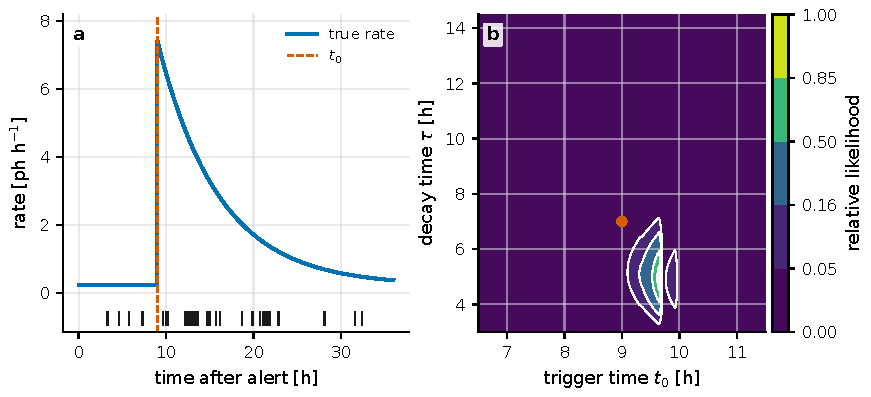
\includegraphics[width=0.92\linewidth]{figures/generated/chapter_13/ch13_transient_event_likelihood.pdf}
\caption{非齐次泊松事件表怎样约束触发时间和衰减时间。左图里每根竖线是一个光子的到达时刻，蓝线是率模型 \(\lambda(t)\)；右图把同一份事件表写成 \(t_0\) 和 \(\tau\) 的相对似然面。少数几个早期光子会\textbf{强烈}地卡住 \(t_0\)，而晚期背景决定 \(\tau\) 会不会被高估——正是式 \eqref{eq:e20-poisson-likelihood} 那"一奖一罚"两项在起作用。}
\label{fig:e20-event-likelihood}
\end{figure}

\section{瞬变源的光子统计与相干性}
\label{sec:e20-coherence}

现在回到本书的老本行——光子统计。瞬变源发的到底是什么样的光？这决定了我们能不能对它用第 \ref{chap:e08} 章的相干函数、第 \ref{chap:e10} 章的强度干涉。

绝大多数瞬变的"连续谱脸面"是\textbf{热的、混沌的}（thermal / chaotic）：新星、超新星、千新星、潮汐瓦解事件的早期光谱都能用一个黑体光球近似（见后文式 \eqref{eq:e20-kilonova-blackbody}）。对这种光，第 \ref{chap:e08} 章给过 Siegert 关系
\[
  g^{(2)}(\tau)=1+\zeta\,|g^{(1)}(\tau)|^2,
\]
即光子会在相干时间内"扎堆"（bunching）。而相干时间由带宽定，第 \ref{chap:e02} 章给过 \(\tau_c\simeq 1/\Delta\nu\)。这里有个对瞬变观测极其现实的数量级：一个宽带光学光球，\(\Delta\nu\) 动辄 \(10^{13}\,\mathrm{Hz}\) 量级，于是 \(\tau_c\sim10^{-13}\,\mathrm{s}\)，只有百飞秒。也就是说，光子扎堆这件事发生在\textbf{飞秒}尺度，而你用来画光变的时间箱是毫秒。在毫秒箱里，扎堆早被平均干净，计数统计退化成纯泊松——每箱涨落就是 \(\sqrt N\) 的散粒噪声（第 \ref{chap:e03} 章）。

这个结论有两面。一面是安慰：做瞬变\textbf{测光}时，只要按泊松误差处理计数就够了，式 \eqref{eq:e20-poisson-likelihood} 的整套推断是自洽的。另一面是提醒：热瞬变源的相干信息藏在飞秒尺度，只有把时间分辨率推到纳秒乃至皮秒的\textbf{强度干涉}才能碰到它。而强度干涉的统计精度，由相关窗口里积攒的\textbf{光子对数}决定：
\begin{equation}
  N_{\rm pair}\simeq r_1 r_2\,\Delta t\,T,
  \qquad
  \delta C\simeq N_{\rm pair}^{-1/2},
  \label{eq:e20-pair-statistics}
\end{equation}
\begin{formulaexplain}
\(N_{\rm pair}\) 是相关窗口 \(\Delta t\) 内、总积分时间 \(T\) 里两台望远镜（率 \(r_1,r_2\)）攒到的光子对数；\(\delta C\) 是纯泊松下的相关测量误差，按对数的平方根下降。
\end{formulaexplain}
其中 \(r_1,r_2\) 是两站的事件率（\(\mathrm{s^{-1}}\)），\(\Delta t\) 是相关时间窗（s），\(T\) 是累计时间（s），\(N_{\rm pair}\) 无量纲。代入一组真实数字：\(r_1=r_2=10^6\,\mathrm{s^{-1}}\)、\(\Delta t=100\,\mathrm{ps}=10^{-10}\,\mathrm{s}\)、\(T=1\,\mathrm{h}=3600\,\mathrm{s}\)，则
\[
  N_{\rm pair}\simeq (10^6)(10^6)(10^{-10})(3600)=3.6\times10^{5},
  \qquad
  \delta C\simeq (3.6\times10^5)^{-1/2}\approx1.7\times10^{-3}.
\]
也就是说一小时能把相关测到千分之一量级——但请注意，这只是\textbf{统计下限}。真实误差还要叠上时间同步误差、死时间（dead time）、光谱带宽、偏振泄漏和背景起伏。对转瞬即逝的源，\(T\) 本身被爆发寿命卡死，这条式子立刻告诉你"能不能在源消失前攒够对数"，是一道硬约束。

还有一小类瞬变，发的根本不是热光，而是\textbf{相干辐射}（coherent emission）：FRB 和脉冲星的射电脉冲就是代表。判据是\textbf{亮温度}（brightness temperature）\(T_b\)——把观测到的亮度按瑞利--金斯律换算成"若是热辐射需要多高的温度"。在射电波段，光子能量远小于热能（\(h\nu\ll k_{\rm B}T_b\)），第 \ref{chap:e05}、\ref{chap:e16} 章用过的单模占有数退化成一个大数：
\[
  \bar n_\nu=\big[\exp(h\nu/k_{\rm B}T_b)-1\big]^{-1}
  \;\xrightarrow[h\nu\ll k_{\rm B}T_b]{}\;
  \frac{k_{\rm B}T_b}{h\nu}\gg1 .
\]
这里用到 \(e^x-1\approx x\)（\(x\to0\)）这一标准泰勒展开，令 \(x=h\nu/k_{\rm B}T_b\) 即得。所以"射电占有数很大"本身一点也不稀奇：\(k_{\rm B}/h\approx2.08\times10^{10}\,\mathrm{Hz\,K^{-1}}\)，只要 \(T_b\gg h\nu/k_{\rm B}\)（\(\nu=1\,\mathrm{GHz}\) 时不过 \(0.05\,\mathrm{K}\)），几乎所有热射电源就都落在 \(\bar n_\nu\gg1\) 的经典高占有数区（\(\nu=1\,\mathrm{GHz}\)、\(T_b=10^4\,\mathrm{K}\) 时 \(\bar n_\nu\sim2\times10^5\)）。可见占有数大小不是干净判据。真正的判据是亮温度\textbf{有没有上限}：任何\textbf{非相干}（incoherent）辐射机制的 \(T_b\) 都被\textbf{逆康普顿灾变}（inverse Compton catastrophe）封顶在 \(T_b\sim10^{12}\,\mathrm{K}\) 量级——再亮，相对论电子就会被自己刚发出的同步光子反复逆康普顿散射，在极短时间里把能量耗散殆尽，亮度升不上去。而 FRB 用观测流量、毫秒时标和源距反推出的亮温度高到 \(T_b\sim10^{35\text{--}40}\,\mathrm{K}\)，比这个上限高出二十多个数量级；对应的 \(\bar n_\nu\propto T_b\) 也远超任何非相干过程能达到的值。这只能意味着大量电荷在同一相位上一起辐射——像激光/脉泽那样的相干过程，而不是一颗颗独立粒子各辐射各的。对这种源，"光子扎堆"不再是弱效应，而是发射机制本身。识别它、并把它和背景、和仪器伪迹区分开，同样只能靠事件表里那份精确到亚毫秒的时间与偏振标签 \citep{2020Natur.587...59B,2020Natur.587...54C,2020Natur.581..391M}。

\section{膨胀的火球：把速度、时间、角尺度连成一把量天尺}
\label{sec:e20-expansion}

许多瞬变（新星、超新星、千新星）在物理上是同一幅画面：一团\textbf{按速度分层膨胀的抛射物}（ejecta）。外层快、内层慢，早期光球在最外的光学厚层，随时间往里退。若膨胀近似\textbf{均匀自相似}（homologous），即半径与速度满足 \(r=v(t-t_0)\)，那么它张开的角半径就把"速度、时间、距离"三件事拴在一起：
\begin{equation}
  \theta(t)=\frac{v_{\rm exp}(t-t_0)}{D}
  =
  5.8\,{\rm mas}
  \left(\frac{v_{\rm exp}}{10^8\,{\rm cm\,s^{-1}}}\right)
  \left(\frac{t-t_0}{10\,{\rm d}}\right)
  \left(\frac{D}{1\,{\rm kpc}}\right)^{-1}.
  \label{eq:e20-angular-expansion}
\end{equation}
\begin{formulaexplain}
\(\theta(t)\) 是膨胀源的角半径，\(v_{\rm exp}\) 是膨胀速度，\(D\) 是距离，\(t_0\) 是爆发时刻。物理很朴素：物质走了多远（\(v_{\rm exp}(t-t_0)\)），除以离我们多远（\(D\)），就是张开多大的角。
\end{formulaexplain}
把那个 \(5.8\,\mathrm{mas}\) 的系数算给你看，别让它凭空冒出来：取 \(v_{\rm exp}=10^8\,\mathrm{cm\,s^{-1}}\)、\(t-t_0=10\,\mathrm{d}=8.64\times10^5\,\mathrm{s}\)，则线半径 \(v_{\rm exp}(t-t_0)=8.64\times10^{13}\,\mathrm{cm}\)；距离 \(D=1\,\mathrm{kpc}=3.086\times10^{21}\,\mathrm{cm}\)。相除得 \(\theta=2.80\times10^{-8}\,\mathrm{rad}\)。再用 \(1\,\mathrm{rad}=2.063\times10^{8}\,\mathrm{mas}\) 换算：\(\theta=2.80\times10^{-8}\times2.063\times10^{8}\approx5.8\,\mathrm{mas}\)。数量级由此落地：银河系新星（\(D\sim1\text{--}5\,\mathrm{kpc}\)、\(v_{\rm exp}\sim10^8\,\mathrm{cm\,s^{-1}}\)）几天到几十天就能爬到毫角秒；而 Ia 型超新星虽然 \(v_{\rm exp}\sim10^9\,\mathrm{cm\,s^{-1}}\) 快十倍，却因为在 \(10\text{--}100\,\mathrm{Mpc}\) 外，十天角半径只有数微角秒；GW170817 那类千新星速度高达 \(0.1\text{--}0.3c\)，但 \(40\,\mathrm{Mpc}\) 的距离仍把早期角尺度压到微角秒以下。

\begin{figure}[tbp]
\centering
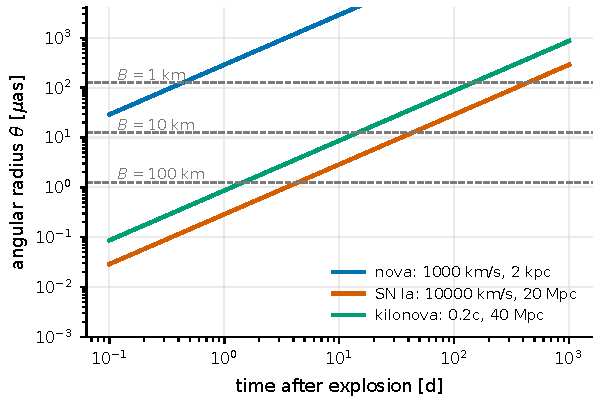
\includegraphics[width=0.92\linewidth]{figures/generated/chapter_13/ch13_expanding_fireball_resolution.pdf}
\caption{膨胀源的角半径由速度、时间、距离共同决定。银河系新星速度虽低，但胜在近，最快进入毫角秒；低红移 Ia 型超新星和千新星速度更高，却因太远而落在微角秒。水平虚线是 \(\lambda=0.5\,\mu\mathrm{m}\) 时不同光学基线的 \(\lambda/B\) 分辨标度——它划出了"谁能被现有干涉仪分辨"的门槛。}
\label{fig:e20-expansion}
\end{figure}

式 \eqref{eq:e20-angular-expansion} 里的 \(v_{\rm exp}\) 从哪来？从谱线。谱线把视向速度投影到波长上：
\begin{equation}
  v_{\rm los}\simeq c\,\frac{\lambda_{\rm obs}-\lambda_0}{\lambda_0},
  \label{eq:e20-doppler-line}
\end{equation}
\begin{formulaexplain}
\(v_{\rm los}\) 是视向速度，\(\lambda_0\) 是实验室波长，\(\lambda_{\rm obs}\) 是观测波长。谱线相对实验室位置移了多少，就把抛射物的速度层"印"在了波长轴上。
\end{formulaexplain}
这里 \(v_{\rm los}\)、\(c\) 单位相同（\(\mathrm{cm\,s^{-1}}\)），\(\lambda\) 是波长（cm 或 \(\text{\AA}\)）。要小心的是：P-Cygni 吸收的蓝端往往代表\textbf{最外层最快}的物质，吸收最低点更接近光学深度最大的那层，而发射线半宽混了几何、光学深度、密度分布好几种效应。若能对每条谱线通道都测出角尺度，数据就变成一组 \(\theta(v_{\rm los})\)——它能区分球壳、双锥、赤道环还是极向风。

角尺度怎么"测"？在强度干涉里，一个圆对称均匀光盘的二阶相关给出可见度模平方 \(|V|^2\)，其一阶可见度模长是熟悉的 Airy 形式（第 \ref{chap:e11} 章）：
\begin{equation}
  |V(B)|=
  \left|
  \frac{2J_1(\pi B\Theta/\lambda)}{\pi B\Theta/\lambda}
  \right|,
  \label{eq:e20-uniform-disk-visibility}
\end{equation}
\begin{formulaexplain}
\(|V(B)|\) 是均匀圆盘的可见度模长，\(\Theta=2\theta\) 是角直径，\(B\) 是投影基线，\(\lambda\) 是波长，\(J_1\) 是一阶贝塞尔函数。基线越长、源越大，可见度掉得越快——这正是"分辨"的定量含义。
\end{formulaexplain}
式中 \(J_1\) 是一阶贝塞尔函数（这是圆孔径衍射的标准结果，第一个零点在辐角 \(3.83\) 处），\(\Theta\) 是角直径（rad），\(B\) 是基线（cm），\(\lambda\) 是波长（cm）。它假设圆对称、单波长、无强临边昏暗；真实新星和超新星常需要薄壳、环、椭球或多组分模型。把角膨胀式 \eqref{eq:e20-angular-expansion} 和谱线速度式 \eqref{eq:e20-doppler-line} 合在一起，就得到一把不依赖标准烛光的量天尺——\textbf{膨胀视差}（expansion parallax）：
\begin{equation}
  D=\frac{v_{\rm exp}(t-t_0)}{\theta(t)}.
  \label{eq:e20-expansion-parallax}
\end{equation}
\begin{formulaexplain}
\(D\) 是几何距离：线速度乘时间得到线半径，除以量到的角半径 \(\theta(t)\)，就是距离。它的前提是——\(v_{\rm exp}\) 和 \(\theta\) 必须对应\textbf{同一层物质}。
\end{formulaexplain}
这是式 \eqref{eq:e20-angular-expansion} 的简单反解，但那个前提是全部风险所在：若谱线量的是外层高速吸收，角尺度却来自连续谱光球（更靠内、更慢），你就在拿两个不同速度层做比，距离会被系统性地带偏。经典新星本身是白矮星表面的热核爆发，抛射质量 \(10^{-5}\text{--}10^{-4}M_\odot\)、速度超过 \(10^3\,\mathrm{km\,s^{-1}}\)；自从 Fermi 发现新星是 GeV \(\gamma\) 射线源，物理图像更被改写成双流结构：慢而密的赤道抛射被双星轨道塑形，快的极向风撞上它、在内激波里加速粒子。V959\,Mon 的 \(\gamma\) 射线持续约 \(12\,\mathrm{d}\)，高分辨射电成像显示激波正位于极向流与赤道物质的交界，热抛射质量约 \(4\times10^{-5}M_\odot\)——在这种源里 \(v_{\rm exp}\) 本就含两个速度组分，谱线、射电图像和光子事件表必须联合拟合 \citep{2014Natur.514..339C,2014Sci...345..554A}。

Ia 型超新星走的是另一条路：先用光变宽度校正成标准烛光。Phillips 关系用 \(B\) 波段衰减率 \(\Delta m_{15}(B)\) 校正峰值绝对星等，宇宙学应用再把校正后的距离模数写成
\begin{equation}
  \mu = m_B - M_B + \alpha x_1-\beta C+\Delta_{\rm host},
  \label{eq:e20-snia-distance-modulus}
\end{equation}
\begin{formulaexplain}
\(\mu\) 是距离模数，\(m_B,M_B\) 是观测与标准化峰值星等，\(x_1\) 是光变宽度，\(C\) 是颜色，\(\alpha,\beta,\Delta_{\rm host}\) 由样本拟合。Ia 标准化，本质上是在一点点修正光度。
\end{formulaexplain}
其中 \(m_B,M_B\) 是星等（无量纲），\(x_1,C\) 无量纲，\(\Delta_{\rm host}\) 是宿主星系相关的修正项。近邻样本 \(m_B\sim10\text{--}16\) 的 Ia 用小望远镜就能拿到高信噪光变，宇宙学样本常在 \(m_B\sim22\text{--}25\)。如果哪天能\textbf{同时}测到角膨胀，就能用式 \eqref{eq:e20-expansion-parallax} 的几何距离去交叉检验这条光度距离——这很难，因为十几天的 Ia 角直径只有微角秒量级，在长基线光学强度干涉里属于"难度极高但收益明确"的目标 \citep{1993ApJ...413L.105P,1998AJ....116.1009R,1999ApJ...517..565P}。

抛射到底圆不圆？看偏振。归一化 Stokes 参数给出线偏振度：
\begin{equation}
  q=\frac{Q}{I},\qquad
  u=\frac{U}{I},\qquad
  P=\sqrt{q^2+u^2},
  \label{eq:e20-stokes-polarization}
\end{equation}
\begin{formulaexplain}
\(q,u\) 是用总强度 \(I\) 归一化的 Stokes 参数，\(P\) 是线偏振度。若抛射完美球对称，各方向散射相消，\(P\to0\)；一旦出现 \(P\neq0\)，就说明有非球对称几何。
\end{formulaexplain}
\(q,u,P\) 都无量纲，通常用百分数报告。SN\,1999by 在极大附近有 \(P\simeq0.3\text{--}0.8\%\)，Si\,II\,\(6150\,\text{\AA}\) 附近还有约 \(0.4\%\) 的偏振变化，模型指向约 \(20\%\) 的整体非球对称，且硅层与连续谱大体共享同一对称轴 \citep{2001ApJ...556..302H}。于是 \(\theta(t)\)（来自光球形状）、\(v_{\rm exp}\)（来自速度层）、\(P(t,\lambda)\)（来自散射几何）三者应被塞进同一个几何模型里解释——这正是"保留频率与偏振标签"在这一类源上的兑现。

最后是超新星最早、最快的那扇窗——\textbf{激波突破}（shock breakout）。激波离表面还有一段深度 \(d\) 时，辐射会先扩散出来形成前驱。令局部密度 \(\rho\)、\textbf{不透明度}（opacity）\(\kappa\)（单位 \(\mathrm{cm^2\,g^{-1}}\)，电子散射下约 \(0.2\text{--}0.4\)，含重元素时可达十的量级），光学深度 \(\tau\simeq\kappa\rho d\)。突破发生在"辐射扩散终于追上动力学时间"的一刻：
\begin{equation}
  t_{\rm diff}\simeq \frac{\tau d}{c}\simeq \frac{d}{v_s},
  \qquad
  \tau\simeq \frac{c}{v_s},
  \label{eq:e20-shock-breakout-condition}
\end{equation}
\begin{formulaexplain}
\(t_{\rm diff}\) 是光子扩散出深度 \(d\) 所需时间，\(v_s\) 是激波速度。光子在光学深度 \(\tau\) 的介质里要走 \(\tau\) 次随机步，扩散时间约 \(\tau d/c\)；当它等于激波穿过 \(d\) 的时间 \(d/v_s\)，辐射就"漏"出来了，给出突破判据 \(\tau\simeq c/v_s\)。
\end{formulaexplain}
把两个时间尺度令相等即得右式，逻辑零跳步：\(\tau d/c = d/v_s\Rightarrow\tau=c/v_s\)。对红超巨星 \(v_s\sim1\text{--}2\times10^9\,\mathrm{cm\,s^{-1}}\)，于是 \(\tau=c/v_s\sim15\text{--}30\)，早期能量主要出现在极紫外或软 X 射线，光学发现常滞后数天。SNLS-04D2dc 的 GALEX 紫外数据就抓到了激波到表面前的前驱，约束了包层结构和前身星半径 \citep{2008Sci...321..223S,2011ApJ...727..104C}。这种小时级的早期信号，直接把压力压回到触发系统：从报警、转向、目标确认到第一轮曝光的总延迟，必须比信号演化还短——这正是本章末尾要量化的东西。

\section{千新星：把多信使延迟变成物理约束}
\label{sec:e20-kilonova}

2017 年的 GW170817 给了瞬变天文学一根教科书式的时间轴。引力波定出双中子星并合的时刻和距离；Fermi/GBM 与 INTEGRAL 在约 \(1.74\pm0.05\,\mathrm{s}\) 后看到 GRB\,170817A；十几个小时内光学对应体被定位；随后 UV/光学/近红外的颜色从蓝飞快转红 \citep{2017PhRvL.119p1101A,2017ApJ...848L..13A,2017ApJ...848L..12A,2017ApJ...848L..17C,2017Natur.551...75S}。把这几路信使缝成一个事件，靠的就是\textbf{时间}。

多信使延迟的定义朴素得几乎像废话：
\begin{equation}
  \Delta t_{a-b}=t_a-t_b .
  \label{eq:e20-mm-delay}
\end{equation}
\begin{formulaexplain}
\(\Delta t_{a-b}\) 是两个信使（或两个波段）的到达时间差。它有意义的前提只有一个：\(t_a\) 和 \(t_b\) 必须在\textbf{同一套时标系统}里测出来。
\end{formulaexplain}
这个前提正是第 \ref{chap:e13} 章那套统一时钟的价值所在：不同望远镜、不同信使，各自的本地时钟若不先归到同一时标，相减出来的 \(1.74\,\mathrm{s}\) 就毫无物理可言。而一旦时标统一了，解释这个 \(\Delta t\) 又必须拆成三块，绝不能囫囵吞下：
\begin{equation}
  \Delta t_{\rm obs}
  =
  \Delta t_{\rm engine}
  +
  \Delta t_{\rm prop}
  +
  \Delta t_{\rm clock}.
  \label{eq:e20-delay-budget}
\end{equation}
\begin{formulaexplain}
观测延迟 \(\Delta t_{\rm obs}\) = 源内发射延迟 \(\Delta t_{\rm engine}\)（并合到喷流突破要多久）+ 传播延迟 \(\Delta t_{\rm prop}\)（路上跑得快慢）+ 时钟/处理误差 \(\Delta t_{\rm clock}\)。三者混淆，就会把源的物理误当成新的传播效应。
\end{formulaexplain}
只有把 \(\Delta t_{\rm engine}\) 和 \(\Delta t_{\rm clock}\) 先扣干净，剩下的 \(\Delta t_{\rm prop}\) 才谈得上约束"引力波与光速是否相同"这类基本问题。若源距 \(D\) 已知，可容许的传播速度差的量级是
\begin{equation}
  \frac{|\Delta v|}{c}
  \lesssim
  \frac{|\Delta t_{\rm prop}|}{D/c}
  =
  2.4\times10^{-16}
  \left(\frac{\Delta t_{\rm prop}}{1\,{\rm s}}\right)
  \left(\frac{D}{40\,{\rm Mpc}}\right)^{-1}.
  \label{eq:e20-speed-difference}
\end{equation}
\begin{formulaexplain}
\(|\Delta v|/c\) 是两信使相对速度差的量级，\(D/c\) 是光行时。距离越远，光行时越长，同样一秒的传播延迟就对应越小的速度差——远方成了极其灵敏的"速度天平"。
\end{formulaexplain}
把系数验一下：\(D=40\,\mathrm{Mpc}=1.234\times10^{26}\,\mathrm{cm}\)，光行时 \(D/c=1.234\times10^{26}/3\times10^{10}=4.11\times10^{15}\,\mathrm{s}\)，故 \(1\,\mathrm{s}/(D/c)=2.4\times10^{-16}\)。这条式子的\textbf{用法}要拿捏准：绝不能把整整 \(1.74\,\mathrm{s}\) 当成传播延迟塞进去，因为 GRB 的发射本身可能就晚于并合（那属于 \(\Delta t_{\rm engine}\)）。它真正的作用，是把"任何未知新传播效应"锁进 \(\sim10^{-16}\) 这个量级的笼子里。

\begin{figure}[tbp]
\centering
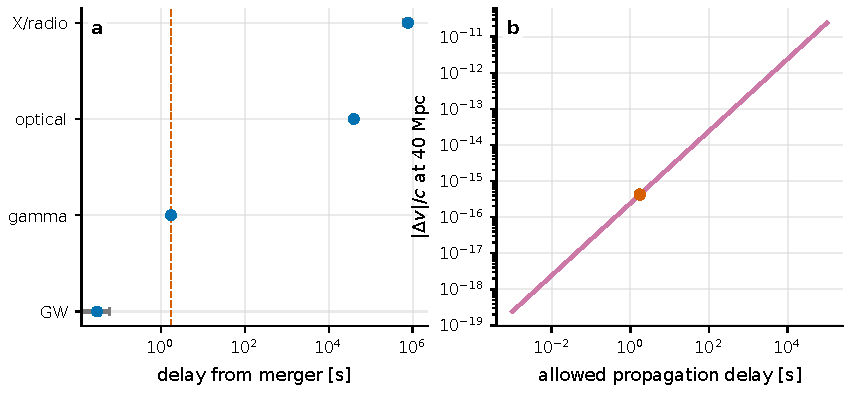
\includegraphics[width=0.92\linewidth]{figures/generated/chapter_13/ch13_multimessenger_delay.pdf}
\caption{多信使延迟的两种读法。左图比较并合后各通道的到达时间：引力波与 \(\gamma\) 射线在秒尺度，光学对应体受定位和昼夜周期限制、常在小时尺度，X 射线/射电则在天到月尺度浮现。右图把传播延迟换算成 \(40\,\mathrm{Mpc}\) 上的 \(|\Delta v|/c\) 量级——源内发射延迟越不确定，能给出的传播约束就越保守。}
\label{fig:e20-mm-delay}
\end{figure}

千新星（kilonova）的光从哪来？来自富中子抛射物里 \(r\)-过程（\(r\)-process）放射性衰变的热化。一个常用标度是
\begin{equation}
  \dot q(t)\simeq
  2\times10^{10}
  \left(\frac{t}{1\,{\rm d}}\right)^{-1.3}
  {\rm erg\,s^{-1}\,g^{-1}},
  \label{eq:e20-rprocess-heating}
\end{equation}
\begin{formulaexplain}
\(\dot q(t)\) 是 \(r\)-过程物质的单位质量加热率，随时间近似按 \(t^{-1.3}\) 衰减。千新星的能源不是余温、不是复合，而是这一路放射性衰变。
\end{formulaexplain}
\(\dot q\) 单位是 \(\mathrm{erg\,s^{-1}\,g^{-1}}\)。真正进入光度的是 \(\epsilon_{\rm th}M_{\rm ej}\dot q\)，其中热化效率 \(\epsilon_{\rm th}<1\)、\(M_{\rm ej}\) 是抛射质量。光变何时到峰，由\textbf{扩散时标}决定——光子要从抛射物内部扩散出来，抛射越厚、越慢、不透明度越大，出来得越晚：
\begin{equation}
  t_{\rm pk}\simeq
  \left(\frac{\kappa M_{\rm ej}}{4\pi v_{\rm ej}c}\right)^{1/2}
  =
  0.6\,{\rm d}
  \left(\frac{\kappa}{0.5\,{\rm cm^2\,g^{-1}}}\right)^{1/2}
  \left(\frac{M_{\rm ej}}{0.01M_\odot}\right)^{1/2}
  \left(\frac{v_{\rm ej}}{0.3c}\right)^{-1/2}.
  \label{eq:e20-kilonova-diffusion}
\end{equation}
\begin{formulaexplain}
\(t_{\rm pk}\) 是千新星峰值时间，\(\kappa\) 是不透明度，\(M_{\rm ej}\) 是抛射质量，\(v_{\rm ej}\) 是速度。不透明度越大、质量越大、速度越低，峰值越晚、颜色越红。
\end{formulaexplain}
把 \(0.6\,\mathrm{d}\) 的系数验一遍：\(\kappa=0.5\,\mathrm{cm^2\,g^{-1}}\)、\(M_{\rm ej}=0.01M_\odot=1.99\times10^{31}\,\mathrm{g}\)、\(v_{\rm ej}=0.3c=9\times10^9\,\mathrm{cm\,s^{-1}}\)、\(c=3\times10^{10}\,\mathrm{cm\,s^{-1}}\)。分子 \(\kappa M_{\rm ej}=9.95\times10^{30}\)，分母 \(4\pi v_{\rm ej}c=4\pi\times9\times10^9\times3\times10^{10}=3.39\times10^{21}\)，比值 \(2.93\times10^{9}\,\mathrm{s^2}\)，开方得 \(5.4\times10^4\,\mathrm{s}\approx0.63\,\mathrm{d}\)。数量级于是清晰：lanthanide 贫的抛射 \(\kappa\sim0.3\text{--}1\,\mathrm{cm^2\,g^{-1}}\)，峰值一天左右且偏蓝；lanthanide 富的抛射 \(\kappa\sim5\text{--}30\,\mathrm{cm^2\,g^{-1}}\)，峰值推到几天乃至十天并转向近红外。

早期光谱能用黑体近似，一步把颜色演化翻译成半径和温度：
\begin{equation}
  L_{\rm bol}=4\pi R_{\rm BB}^2\sigma_{\rm SB}T_{\rm BB}^4 .
  \label{eq:e20-kilonova-blackbody}
\end{equation}
\begin{formulaexplain}
\(L_{\rm bol}\) 是总辐射光度，\(R_{\rm BB},T_{\rm BB}\) 是黑体半径和温度，\(\sigma_{\rm SB}\) 是 Stefan–Boltzmann 常数。给定 SED，拟合出 \(R_{\rm BB},T_{\rm BB}\)，就把"颜色随时间变"翻成了"发光面在膨胀、在降温"。
\end{formulaexplain}
GW170817 在约 \(0.6\,\mathrm{d}\) 时可用 \(T_{\rm BB}\simeq8300\,\mathrm{K}\)、\(R_{\rm BB}\simeq4.5\times10^{14}\,\mathrm{cm}\)、\(L_{\rm bol}\simeq5\times10^{41}\,\mathrm{erg\,s^{-1}}\) 描述，对应 \(v\simeq0.3c\)。随后 SED 迅速偏离单一黑体：紫外/蓝光衰减、近红外相对增强。这逼出至少两组分模型——蓝组分 \(M_{\rm ej}\sim0.01M_\odot\)、\(v\sim0.27\text{--}0.3c\)，红组分 \(M_{\rm ej}\sim0.04M_\odot\)、\(v\sim0.1c\)；三组分模型还会把中间 opacity 的"紫组分"单列出来 \citep{2017Natur.551...75S,2017ApJ...848L..17C,2017ApJ...848L..27T,2017Sci...358.1565E}。单一组分解释不了"早蓝晚红"，这本身就是数据在告诉我们抛射有结构。

\begin{figure}[tbp]
\centering
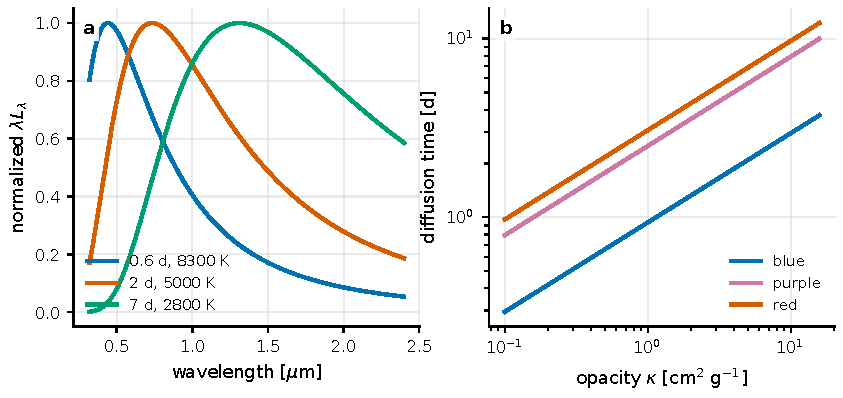
\includegraphics[width=0.92\linewidth]{figures/generated/chapter_13/ch13_kilonova_color_evolution.pdf}
\caption{千新星从蓝到红的演化。左图用三个黑体 SED 展示温度降低后峰值波长向红外移动（维恩位移）；右图用扩散时标式 \eqref{eq:e20-kilonova-diffusion} 显示 opacity 越大、质量越大、速度越低，峰值越晚。GW170817 的蓝组分快而低 opacity、红组分慢而高 opacity，故单一抛射组分无法同时解释早期蓝光和晚期近红外。}
\label{fig:e20-kilonova}
\end{figure}

引力波还额外奉送一件宝物——\textbf{标准汽笛}（standard siren）：并合波形的振幅直接给出光度距离，不需要距离阶梯。低红移下可粗略写成
\begin{equation}
  H_0\simeq \frac{cz_{\rm host}}{D_L},
  \label{eq:e20-standard-siren}
\end{equation}
\begin{formulaexplain}
\(H_0\) 是 Hubble 常数，\(z_{\rm host}\) 是宿主星系红移，\(D_L\) 是引力波给出的光度距离。红移（膨胀速度）除以距离，就是膨胀率——只是这里的距离来自引力波，不来自烛光。
\end{formulaexplain}
\(z_{\rm host}\) 无量纲，\(D_L\) 单位是 cm 或 Mpc，\(H_0\) 单位是 \(\mathrm{km\,s^{-1}\,Mpc^{-1}}\)。GW170817 的主要退化来自倾角与距离：正对我们的双星既更亮、又更难定倾角。电磁对应体在这里立了大功——它给出宿主、红移、喷流视角和抛射几何，替引力波破掉一部分退化。这就是多信使的精髓：同一个物理事件，被引力波、\(\gamma\) 射线、光学各投影成一个侧面，再由一个联合似然把它们缝回一个三维的真相。

\section{伽马暴余辉：把喷流几何写进光变斜率}
\label{sec:e20-grb}

伽马暴的 prompt emission 给出高能触发，\textbf{余辉}（afterglow）才是能被慢慢追踪的外激波物理。一个相对论薄壳撞进外部介质后，观测时刻 \(t\) 与激波半径 \(R\)、洛伦兹因子 \(\Gamma\) 的关系近似为
\begin{equation}
  t\simeq \frac{(1+z)R}{4\Gamma^2c}.
  \label{eq:e20-grb-arrival-time}
\end{equation}
\begin{formulaexplain}
\(t\) 是观测到达时刻，\(R\) 是激波半径，\(\Gamma\) 是洛伦兹因子，\(z\) 是红移。因子 \(1/\Gamma^2\) 是相对论 beaming 与光行时效应叠加的结果：源跑得几乎和自己发的光一样快，把很大的 \(R\) 压进极短的观测时间。
\end{formulaexplain}
这条式子的震撼在那个 \(\Gamma^2\)：典型早期余辉 \(\Gamma\sim10\text{--}300\)、\(R\sim10^{16}\text{--}10^{18}\,\mathrm{cm}\)，可光学信号能在触发后几十秒到几分钟就进入望远镜视场——一个天文尺度的半径，被压缩成一次快到需要机器人望远镜才追得上的观测 \citep{1997ApJ...476..232M,1998ApJ...497L..17S,1998Natur.395..670G,1999PhR...314..575P,2004RvMP...76.1143P,2006ARA&A..44..507W}。

余辉的光来自激波加速的电子做同步辐射。设电子能谱是幂律：
\begin{equation}
  N(\gamma_e)\,d\gamma_e \propto \gamma_e^{-p}\,d\gamma_e,
  \qquad \gamma_e>\gamma_m,
  \label{eq:e20-electron-powerlaw}
\end{equation}
\begin{formulaexplain}
\(N(\gamma_e)\) 是电子洛伦兹因子的分布，\(p\) 是能谱指数（典型 \(2\text{--}2.5\)），\(\gamma_m\) 是低能截止。同步余辉谱的斜率，最终由这一个数 \(p\) 主宰。
\end{formulaexplain}
观测上通常先把光变和颜色压成两个斜率——时间衰减指数 \(\alpha\) 和谱指数 \(\beta\)：
\begin{equation}
  F_\nu(t)\propto t^{-\alpha}\nu^{-\beta}.
  \label{eq:e20-afterglow-powerlaw}
\end{equation}
\begin{formulaexplain}
\(F_\nu(t)\) 是余辉通量密度，\(\alpha\) 管"随时间怎么暗下去"，\(\beta\) 管"谱怎么随频率倾斜"。两个斜率，是余辉最紧凑的指纹。
\end{formulaexplain}
在均匀介质、绝热、慢冷却且观测频率落在 \(\nu_m<\nu<\nu_c\) 区间时，这两个斜率并不独立，而由同一个 \(p\) 锁死：
\begin{equation}
  \beta=\frac{p-1}{2},
  \qquad
  \alpha=\frac{3(p-1)}{4}.
  \label{eq:e20-closure-relation}
\end{equation}
\begin{formulaexplain}
这是\textbf{闭合关系}（closure relation）：它把观测的 \(\alpha,\beta\) 和电子指数 \(p\) 绑在一起。数据若明显偏离它，就说明"简单介质/弱能量注入/微物理不演化"这些假设里至少有一条塌了。
\end{formulaexplain}
两式相除立刻看出结构：\(\alpha/\beta=3/2\)——一个不含 \(p\) 的定值，是这段区间的硬预言。代入 \(p=2.2\)，得 \(\beta\simeq0.6\)、\(\alpha\simeq0.9\)；若观测频率越到 \(\nu>\nu_c\)（快冷却段），则变为 \(\alpha=(3p-2)/4\)。观测上余辉在爆后一天常为 \(19\text{--}20\) 星等，偏振可达百分之几到约 \(10\%\)，与同步辐射和喷流几何直接相关 \citep{2004RvMP...76.1143P,2006ARA&A..44..507W}。

\begin{figure}[tbp]
\centering
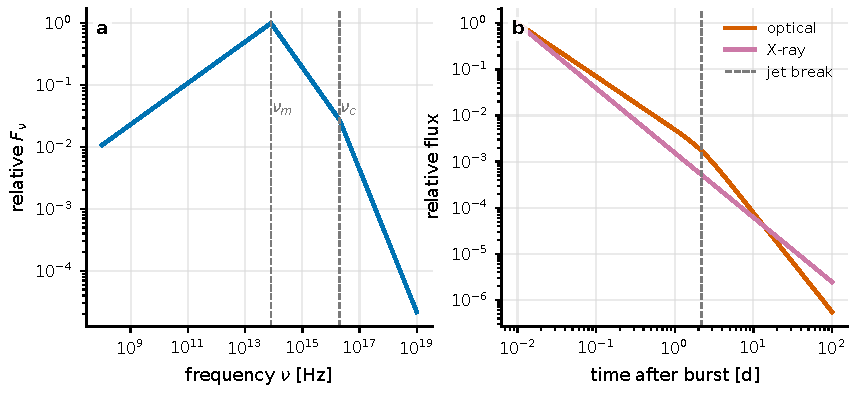
\includegraphics[width=0.92\linewidth]{figures/generated/chapter_13/ch13_afterglow_synchrotron_breaks.pdf}
\caption{伽马暴余辉的同步辐射读法。左图显示特征频率 \(\nu_m\)（最小电子）和 \(\nu_c\)（冷却）把谱切成斜率不同的区间；右图显示喷流 break 前后光变变陡。若光学和 X 射线不在同一谱段，它们的 \(\alpha,\beta\) 不必相同——必须先判断观测频率相对 \(\nu_m,\nu_c\) 的位置，才能套闭合关系。}
\label{fig:e20-afterglow}
\end{figure}

喷流不是各向同性的。当 \(\Gamma\) 衰减到约 \(1/\theta_j\) 时，观测者第一次"看见喷流的边缘"，光变曲线出现\textbf{无色喷流 break}（achromatic jet break）。常用估算是
\begin{equation}
  \theta_j\simeq
  0.10
  \left(\frac{t_j}{1\,{\rm d}}\right)^{3/8}
  \left(\frac{1+z}{2}\right)^{-3/8}
  \left(\frac{E_{\rm iso,52}}{n_0}\right)^{-1/8},
  \label{eq:e20-jet-opening-angle}
\end{equation}
\begin{formulaexplain}
\(\theta_j\) 是喷流半张角（rad），\(t_j\) 是 jet break 时间，\(E_{\rm iso,52}\) 是以 \(10^{52}\,\mathrm{erg}\) 为单位的各向同性能量，\(n_0\) 是外部数密度（\(\mathrm{cm^{-3}}\)）。break 越晚，喷流通常越宽。
\end{formulaexplain}
留意那些\textbf{很弱}的指数——\(3/8\) 和 \(1/8\)。它们是误差传播的好消息：即便 \(E_{\rm iso}\) 或 \(n\) 各自有一个数量级的不确定，\((E_{\rm iso}/n)\) 变化 \(10\) 倍，经过 \(1/8\) 次方也只让 \(\theta_j\) 变约 \(10^{1/8}\approx1.33\) 倍，即三成。真正的风险不在这些参数，而在\textbf{误分类}：色变 break、能量注入、密度跳变、乃至叠加的超新星隆起，都可能被错当成 jet break \citep{2003Natur.423..847H,2004ApJ...611.1005G}。GRB\,980425/SN\,1998bw 和 GRB\,030329/SN\,2003dh 把长暴与宽线 Ic 型超新星联系起来，短暴与双中子星并合的联系则在 GW170817 后成了多信使铁证。伽马暴逼着望远镜系统同时处理秒级高能触发、分钟级光学闪、小时到天的余辉、周到月的射电量能，事件表除了通量，还得替每个阶段留住时间基准与频段衔接。

\section{潮汐瓦解事件：从回落率读出黑洞质量}
\label{sec:e20-tde}

当一颗恒星太靠近超大质量黑洞，它会被撕碎——\textbf{潮汐瓦解事件}（tidal disruption event，TDE）。撕裂发生在潮汐半径以内：
\begin{equation}
  r_t\simeq R_\ast\left(\frac{M_\bullet}{M_\ast}\right)^{1/3},
  \label{eq:e20-tidal-radius}
\end{equation}
\begin{formulaexplain}
\(r_t\) 是潮汐半径，\(M_\bullet\) 是黑洞质量，\(M_\ast,R_\ast\) 是恒星质量和半径。恒星一旦进入 \(r_t\) 以内，黑洞在它两端的引力差就超过它自身的自引力，把它拉成一条面条。
\end{formulaexplain}
\(r_t,R_\ast\) 单位是 cm，\(M_\bullet,M_\ast\) 单位是 g。要不要产生明亮 flare，还得比一个尺度——Schwarzschild 半径：
\begin{equation}
  r_s=\frac{2GM_\bullet}{c^2}.
  \label{eq:e20-schwarzschild-radius-tde}
\end{equation}
\begin{formulaexplain}
\(r_s\) 是黑洞的 Schwarzschild 半径。比较 \(r_t\) 与 \(r_s\)：若 \(r_t\lesssim r_s\)，恒星还没被撕碎就整个吞下去，看不到亮 flare。
\end{formulaexplain}
注意 \(r_t\propto M_\bullet^{1/3}\) 而 \(r_s\propto M_\bullet\)，黑洞越重，\(r_s\) 追得越快。于是主序星 TDE 最常见于 \(M_\bullet\sim10^5\text{--}10^7M_\odot\)，到 \(10^8M_\odot\) 附近，\(r_s\) 逼近甚至越过 \(r_t\)，选择效应变强 \citep{1988Natur.333..523R,2021ARA&A..59...21G}。

被撕碎后，一半碎屑束缚、一半逃逸。最早返回近心点的束缚碎屑给出\textbf{回落时标}：
\begin{equation}
  t_{\rm min}\simeq
  41\,{\rm d}
  \left(\frac{M_\bullet}{10^6M_\odot}\right)^{1/2}
  \left(\frac{M_\ast}{M_\odot}\right)^{-1}
  \left(\frac{R_\ast}{R_\odot}\right)^{3/2}.
  \label{eq:e20-tde-fallback-time}
\end{equation}
\begin{formulaexplain}
\(t_{\rm min}\) 是最束缚碎屑绕回近心点的时间——由最束缚轨道的开普勒周期给出，故按 \(M_\bullet^{1/2}\) 增长。它是 TDE 上升时标的标尺。
\end{formulaexplain}
黑洞越重，\(t_{\rm min}\) 越长（\(\propto M_\bullet^{1/2}\)），所以上升时标（rise time）本身就藏着黑洞质量。回落率随后转入经典的 \(t^{-5/3}\) 衰减：
\begin{equation}
  \dot M_{\rm fb}\simeq
  \frac{M_\ast}{3t_{\rm min}}
  \left(\frac{t}{t_{\rm min}}\right)^{-5/3}.
  \label{eq:e20-tde-fallback-rate}
\end{equation}
\begin{formulaexplain}
\(\dot M_{\rm fb}\) 是碎屑回落率。理想的 \(t^{-5/3}\) 衰减来自碎屑能量的均匀分布，是 TDE 的经典指纹；但观测光度还会被环化（circularization，碎屑轨道相互碰撞、耗散、绕成吸积盘的过程）和再处理磨圆，未必严格照它走。
\end{formulaexplain}
\(\dot M_{\rm fb}\) 常用 \(M_\odot\,\mathrm{yr^{-1}}\)。这个回落有多猛？拿它比 Eddington 吸积率：
\begin{equation}
  \dot M_{\rm Edd}
  =
  \frac{L_{\rm Edd}}{\eta c^2}
  \simeq
  0.022
  \left(\frac{M_\bullet}{10^6M_\odot}\right)
  \left(\frac{\eta}{0.1}\right)^{-1}
  M_\odot\,{\rm yr^{-1}} ,
  \label{eq:e20-eddington-rate}
\end{equation}
\begin{formulaexplain}
\(\dot M_{\rm Edd}\) 是 Eddington 吸积率，\(\eta\) 是辐射效率。把 \(\dot M_{\rm fb}\) 和它比，就知道回落有没有冲进超 Eddington 阶段。
\end{formulaexplain}
把 \(0.022\) 验一下：\(L_{\rm Edd}=1.26\times10^{38}(M_\bullet/M_\odot)\,\mathrm{erg\,s^{-1}}=1.26\times10^{44}\,\mathrm{erg\,s^{-1}}\)（\(10^6M_\odot\)），\(\eta c^2=0.1\times(3\times10^{10})^2=9\times10^{19}\)，故 \(\dot M_{\rm Edd}=1.4\times10^{24}\,\mathrm{g\,s^{-1}}\)；换成 \(M_\odot\,\mathrm{yr^{-1}}\)（乘 \(3.156\times10^7\,\mathrm{s\,yr^{-1}}\)、除 \(1.989\times10^{33}\,\mathrm{g}\)）得 \(0.022\)。对 \(10^6M_\odot\) 黑洞，太阳型恒星的峰值回落率能显著超 Eddington——但\textbf{光学}光度未必同样超，因为 circularization、星风、遮蔽和再处理会把内盘的能量搬到 UV/光学并重新分配。

\begin{figure}[tbp]
\centering
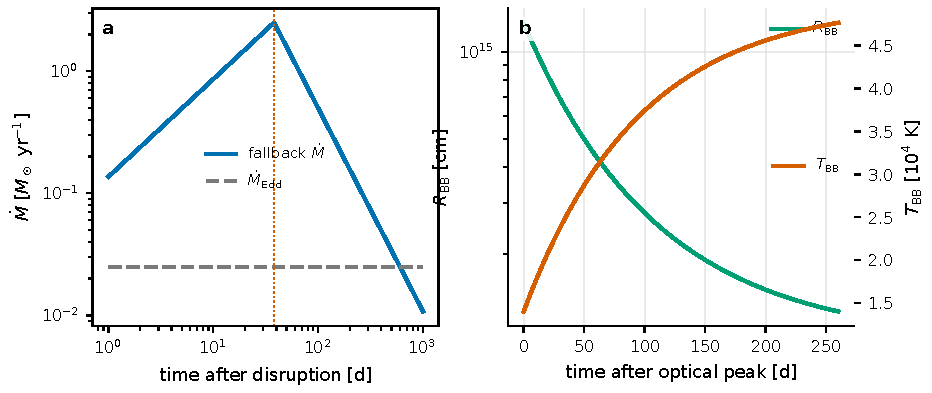
\includegraphics[width=0.92\linewidth]{figures/generated/chapter_13/ch13_tde_fallback_reprocessing.pdf}
\caption{TDE 的回落与再处理。左图显示 \(t^{-5/3}\) 回落在几十天尺度进入衰减段，并可长期高于 \(10^6M_\odot\) 黑洞的 Eddington 吸积率；右图给出光学/UV 黑体光球的一种典型演化：半径从 \(10^{15}\,\mathrm{cm}\) 量级收缩到 \(10^{14}\,\mathrm{cm}\)，温度从 \(10^4\,\mathrm{K}\) 量级升到数 \(10^4\,\mathrm{K}\)。}
\label{fig:e20-tde}
\end{figure}

光学 TDE 的黑体半径通常是 \(10^{14}\text{--}10^{15}\,\mathrm{cm}\)，比 \(10^6M_\odot\) 黑洞的几倍 \(r_s\) 大得多；温度常为几 \(\times10^4\,\mathrm{K}\)，演化比普通超新星慢。AT2018zr 是 ZTF 早期样本里第一个把上升段拍全的 TDE，最早检测约在峰值前 \(50\,\mathrm{d}\)；其黑体温度早期约 \(1.4\times10^4\,\mathrm{K}\)、晚期升到 \(>5\times10^4\,\mathrm{K}\)，半径从 \(10^{15.1}\,\mathrm{cm}\) 降到 \(<10^{14}\,\mathrm{cm}\)，而 X 射线光度比同期光学/UV 黑体低好几个数量级——说明遮蔽或再处理不能忽略 \citep{2019ApJ...872..198V,2021ARA&A..59...21G}。喷流型 TDE（如 Swift\,J1644+57）则把事件表推向高能与快速变率：X 射线剧烈闪烁，射电跟踪外流与介质的相互作用 \citep{2011Sci...333..203B}。至于 TDE 与高能中微子的可能关联，则是又一类需要靠时间、方向和能量三重符合去判断的多信使课题 \citep{2021NatAs...5..510S}。哪怕在这种"慢"瞬变里，事件表仍要留住完整时间信息：判断一个高能事件是不是属于某个光学 flare，靠的还是天球位置、时间延迟、能量、方向误差和源演化是否彼此相容。

\section{机会目标观测：把"快"和"误差"一起算}
\label{sec:e20-tooo}

瞬变观测的成败常由响应速度决定。但"快"必须被量化，否则只是口号。一个实用条件是：从触发到第一组有效曝光的总延迟，要短于你想采样的源演化时标：
\begin{equation}
  t_{\rm alert}+t_{\rm slew}+t_{\rm acq}+t_{\rm exp}
  < f_{\rm samp}\,t_{\rm evol},
  \label{eq:e20-response-budget}
\end{equation}
\begin{formulaexplain}
左边是响应预算：报警发布 \(t_{\rm alert}\) + 望远镜转向 \(t_{\rm slew}\) + 目标确认导星 \(t_{\rm acq}\) + 第一组有效曝光 \(t_{\rm exp}\)；右边是想采样的源演化时标 \(t_{\rm evol}\) 乘一个采样系数 \(f_{\rm samp}\)。机会目标观测（target-of-opportunity）就是要满足这条不等式。
\end{formulaexplain}
若想\textbf{解析}上升段而不只是抓一个点，\(f_{\rm samp}\sim0.1\) 才合理（采样要快过演化十倍）。代入本章各类源：GRB 光学闪的 \(t_{\rm evol}\) 可小于 \(10^3\,\mathrm{s}\)，GW 对应体的蓝光阶段约一天，新星早期的射电/光谱结构在天到周内变化，TDE 的上升时标则常是数十天。同一条式子，把"到底要多快"从情绪变成了可核对的数字。

抢到了目标，还得算曝光够不够深。普通成像的信噪比是
\begin{equation}
  {\rm SNR}=
  \frac{N_s}
  {\left(N_s+N_b+n_{\rm pix}\sigma_{\rm read}^2\right)^{1/2}},
  \label{eq:e20-imaging-snr}
\end{equation}
\begin{formulaexplain}
\({\rm SNR}\) 是成像信噪比，\(N_s\) 是源计数，\(N_b\) 是背景计数，\(n_{\rm pix}\sigma_{\rm read}^2\) 是孔径内像素累加的读出噪声。分母那三项，正是"源自身涨落 + 背景涨落 + 电子学噪声"三种误差的求和。
\end{formulaexplain}
\(N_s,N_b\) 是计数（无量纲），\(n_{\rm pix}\) 是孔径内像素数，\(\sigma_{\rm read}\) 是每像素读出噪声（电子数）。源亮时（\(N_s\gg N_b,\,n_{\rm pix}\sigma_{\rm read}^2\)），分母趋于 \(\sqrt{N_s}\)，回到第 \ref{chap:e03} 章的散粒噪声极限 \({\rm SNR}\to\sqrt{N_s}\)；源暗时，背景和读出噪声接管，这正是深场瞬变难做的原因。

最后，别忘了\textbf{宿主关联}也是有误差的统计判断，不是"看着近就算对上了"。若瞬变定位误差半径为 \(r\)、深度 \(m\) 内背景星系面密度为 \(\Sigma(<m)\)，那么随机撞上一个背景星系的\textbf{偶然重合概率}是
\begin{equation}
  P_{\rm cc}=1-\exp[-\pi r^2\Sigma(<m)].
  \label{eq:e20-chance-coincidence}
\end{equation}
\begin{formulaexplain}
\(P_{\rm cc}\) 是随机宿主重合概率，\(r\) 是定位误差半径，\(\Sigma(<m)\) 是背景星系面密度。它其实是一个泊松结论："误差圆内至少有一个背景星系"的概率 \(1-e^{-\langle N\rangle}\)，其中期望数 \(\langle N\rangle=\pi r^2\Sigma\)。
\end{formulaexplain}
式中 \(r\) 单位是 rad 或 arcsec，\(\Sigma(<m)\) 是单位立体角内的星系数（如 \(\mathrm{arcsec^{-2}}\)），乘积 \(\pi r^2\Sigma\) 无量纲。定位越差、星系越密，\(P_{\rm cc}\) 越大，宿主关联越不可信。GW170817 就是靠 Virgo 探测器加入把天区从上百收缩到几十平方度，才让光学巡天能在同一夜锁定宿主；TDE 则反过来需要亚角秒天体测量，去证明 flare 确实坐在星系核上。同一个 \(P_{\rm cc}\)，从引力波定位一直管到核瞬变认证 \citep{2017PhRvL.119p1101A,2017ApJ...848L..12A,2019ApJ...872..198V}。

把本章六类源的时标、观测量与主要风险并排列出，便于对照：
\begin{longtable}{@{}p{0.14\linewidth}p{0.18\linewidth}p{0.28\linewidth}p{0.28\linewidth}@{}}
\toprule
源类 & 关键时标 & 典型观测量 & 主要风险 \\
\midrule
经典新星 & 天到月 & 谱线速度、射电角尺度、\(\gamma\) 射线窗口 & 多速度组分会偏置膨胀视差。 \\
Ia 型超新星 & 天到周 & 光变宽度、颜色、Si\,II 速度、偏振、微角秒角尺度 & 光度校正与角尺度来自不同物理层。 \\
核心坍缩 & 分钟到天 & UV/软 X 射线暴发、早期光谱、偏振 & 触发太晚会错过前身星半径信息。 \\
千新星 & 小时到十天 & GW 距离、\(\gamma\) 射线延迟、颜色与近红外演化 & opacity、视角与抛射几何相互退化。 \\
伽马暴 & 秒到月 & \(\alpha,\beta\)、jet break、偏振、射电量能 & 色变 break 或能量注入会误判喷流几何。 \\
潮汐瓦解 & 周到年 & 上升时标、核位置、\(T_{\rm BB}\)、\(R_{\rm BB}\)、X/光学比 & AGN 变源污染与再处理几何不唯一。 \\
\bottomrule
\end{longtable}

\section*{本章要点}
\addcontentsline{toc}{section}{本章要点}

\begin{itemize}
  \item \textbf{瞬变的信息在时间里。} 光变曲线是分箱后的产物，会抹掉起始时刻和精细结构；未分箱的非齐次泊松似然式 \eqref{eq:e20-poisson-likelihood} 直接吃事件时刻 \(t_j\)，这正是第 \ref{chap:e13} 章坚持保留每个光子时间/频率/偏振标签的理由。
  \item \textbf{触发是推断，不是报警。} 用几率比式 \eqref{eq:e20-trigger-odds} 把"先验罕见度"和"数据似然"一起放进判断；误触发由泊松尾概率式 \eqref{eq:e20-false-alarm} 控制，但真实假警报数要乘上时间窗、像素、能道、模板的试验次数。
  \item \textbf{瞬变源多是热的混沌光。} 宽带黑体光球的相干时间只有飞秒（\(\tau_c\simeq1/\Delta\nu\)），毫秒箱里计数退化成纯泊松散粒噪声；要碰相干信息得靠纳秒/皮秒的强度干涉，其精度由光子对数式 \eqref{eq:e20-pair-statistics} 决定。FRB、脉冲星那样的相干辐射则以极高亮温度暴露自己。
  \item \textbf{几何把速度、时间、角尺度连成量天尺。} 角膨胀式 \eqref{eq:e20-angular-expansion} 加谱线速度式 \eqref{eq:e20-doppler-line} 给出膨胀视差式 \eqref{eq:e20-expansion-parallax}，但速度与角尺度必须对应同一物质层，否则距离系统偏差。
  \item \textbf{多信使靠时间缝合。} 延迟只有在统一时标下才有意义（式 \eqref{eq:e20-mm-delay}），且必须拆成源内发射、传播、时钟三部分（式 \eqref{eq:e20-delay-budget}）；远距离让秒级延迟对应 \(\sim10^{-16}\) 的速度差约束（式 \eqref{eq:e20-speed-difference}）。
  \item \textbf{"快"要量化，宿主要检验。} 响应预算式 \eqref{eq:e20-response-budget} 把速度变成可核对的不等式；偶然重合概率式 \eqref{eq:e20-chance-coincidence} 提醒我们，宿主关联和触发一样，是带误差的统计判断。第 \ref{chap:e15} 章的误差预算会把这些一并纳入可行性分析。
\end{itemize}

\medskip
\noindent\textbf{想一想}
\begin{itemize}
  \item 一次 GRB 触发用 \(\Delta t=0.05\,\mathrm{s}\) 的窗口、背景率 \(b=2\,\mathrm{s^{-1}}\)。若一夜搜索了 \(10^{9}\) 个独立窗口，要把期望假警报压到 1 次以下，触发阈值 \(n\) 大致该取多少？（提示：用式 \eqref{eq:e20-false-alarm} 先算单窗口 \(P_{\rm FA}\)，再乘试验次数。）
  \item 若某新星谱线给出的是最外层 \(v_{\rm exp}=1.5\times10^8\,\mathrm{cm\,s^{-1}}\)，而角尺度实际来自更靠内、速度只有 \(0.7\) 倍的连续谱光球，用式 \eqref{eq:e20-expansion-parallax} 得到的距离会偏大还是偏小、偏多少？
  \item 为什么对宽带热瞬变做测光时可以放心用 \(\sqrt N\) 误差，而做强度干涉时却必须回到光子对数式 \eqref{eq:e20-pair-statistics}？两者分别在"看"信号的哪个时间尺度？
\end{itemize}


% ============================================================
\part{传播、宇宙学与新物理}
\chapter{传播效应：等离子体、尘埃与引力透镜}
\label{chap:e21}

\begin{chapteropening}
到现在为止，我们几乎都在问同一类问题：\textbf{源本来是什么样子？}——它的角直径、它的相干时间、它的光子统计。可是有一件事我们一直偷偷假设掉了：光从源出发，一路飞到望远镜，中间那几千光年、几十亿光年，是"透明"的。它当然不是。光要穿过稀薄的自由电子、湍动的磁化等离子体、飘着尘埃颗粒的星云、乃至被大质量天体压弯的时空。每穿过一层，它的到达时间、频率、偏振、方向、甚至"有几个副本"都会被悄悄改写。

本章要把这条"路上发生了什么"讲清楚。主线是：先把传播看成一条\textbf{有记忆的通道}（channel with memory）——它不是简单地把信号乘一个常数，而是把每个光子身上的标签重新填一遍。然后我们逐个拆开四类改写者：冷等离子体的\(\nu^{-2}\)色散（我们会一步不跳地推出"为什么低频光子迟到"）、湍流带来的散射与闪烁、尘埃的消光与红化、以及弯曲时空的引力透镜。最后回到本书的老本行：这些效应既\textbf{污染}信号（把相干性抹平、把时间戳拖乱），也\textbf{编码}信号（在色散量里存下电子账本，在时间延迟里存下宇宙学）。它承接第 \ref{chap:e02} 章的带宽与相干时间、第 \ref{chap:e13} 章的时间同步，是把"源端物理"翻译成"探测器事件"的最后一道工序。
\end{chapteropening}

\section{把传播当成一条有记忆的通道}
\label{sec:e21-channel}

先建立画面。最省事的想法是把介质当成一块灰玻璃：光穿过去，暗了一点、红了一点，其余不变。对求平均亮度、平均颜色，这个"乘一个常数"的图像有时够用。但本书关心的是\textbf{事件表}（第 \ref{chap:e13} 章）——每个光子候选带着到达时刻、频率、偏振、方向这几个标签；也关心\textbf{相干性}——不同时刻、不同望远镜之间场的相位关系。对这些量，"灰玻璃"是灾难性的近似，因为传播真正做的事是\textbf{把标签重写}：频率标签决定它迟到多少，偏振标签会被磁场旋转，方向标签被散射打散、被透镜复制，到达时间标签会被多条路径拖出回声。

所以更好的第一步不是问"源本来多亮"，而是问"源端的场要经过怎样一条通道，才变成我探测器上的一次事件"。把它写成线性通道最直接。在时间域里，第 \(i\) 个观测通道（某个偏振、某台望远镜、某个像、某个频道）的电场是源端各通道场的\textbf{卷积叠加}：
\begin{equation}
  E_{{\rm out},i}(t)
  =
  \sum_j\int h_{ij}(t-t')\,E_{{\rm src},j}(t')\,{\rm d}t'
  + n_i(t) .
  \label{eq:e21-channel-time}
\end{equation}
\begin{formulaexplain}
\(E_{{\rm out},i}\) 是第 \(i\) 个观测通道的场，\(E_{{\rm src},j}\) 是第 \(j\) 个源端通道的场，\(h_{ij}\) 是从 \(j\) 到 \(i\) 的响应函数，\(n_i\) 是前景与探测噪声。积分号是关键：传播\textbf{有记忆}——一个源端时刻的光会被延迟、展宽后贡献到许多观测时刻。
\end{formulaexplain}
逐个符号说清楚：\(i,j\) 标记偏振、望远镜、像或频道（无量纲编号）；\(h_{ij}(t-t')\) 是脉冲响应（impulse response），它的量纲取决于场的归一化，但真正用得上的是它的三个特征——\textbf{时间宽度}（信号被展宽多少）、\textbf{峰值延迟}（信号整体迟到多少）、以及不同通道之间的\textbf{相对相位}；\(n_i(t)\) 是前景热辐射、天光背景和探测链噪声之和。如果介质只吸收不散射，\(h_{ij}\) 近似是个对角的、被压低了幅度的 delta 函数；如果有 Faraday 旋转，它会在两个线偏振通道之间"转账"；如果有散射或透镜，它同时把方向和到达时间搅在一起。地球质心改正、钟差、大气延迟、仪器电子延迟，也都是这个 \(h_{ij}\) 的一部分——脉冲星计时（pulsar timing）正是把这些项一项项拆到纳秒量级的最成熟范例 \citep{2006MNRAS.372.1549E}。

翻回事件表的语言：一个光子候选是一行 \((t_q,\nu_q,p_q,\bm{x}_q,w_q)\)——到达时刻 \(t_q\)（单位 s）、频率 \(\nu_q\)（单位 Hz）、偏振通道 \(p_q\)、空间标签 \(\bm{x}_q\)（像素、基线或望远镜编号）、质量权重 \(w_q\)。这一节剩下要做的，就是把式 \eqref{eq:e21-channel-time} 那个抽象的 \(h_{ij}\)，对四类介质各写出一个具体形式，看它到底怎么改这五个标签：色散改 \(t_q(\nu_q)\)，Faraday 旋转改 \(p_q(\lambda_q^2)\)，散射把一个窄脉冲的 \(t_q\) 摊成一条长尾，尘埃改不同 \(\lambda_q\) 被接收的概率，透镜把一个源事件复制成好几组 \((\bm{x}_q,t_q)\)。

在开始之前，先把\textbf{数量级的地图}摊在桌上，这样后面每算一个数字都知道自己站在哪。银河系高银纬方向的色散量（我们马上会定义）常在 \(30\text{--}100\,{\rm pc\,cm^{-3}}\)，而快速射电暴（fast radio burst，FRB）能到 \(10^{3}\text{--}10^{4}\,{\rm pc\,cm^{-3}}\)。普通星际介质的旋转量多为 \(1\text{--}10^{2}\,{\rm rad\,m^{-2}}\)，强磁化致密环境可到 \(10^{4}\text{--}10^{5}\,{\rm rad\,m^{-2}}\)。散射展宽从微秒到秒，低频端涨得极快。光学消光在高银纬常小于 \(0.1\) 星等，在银盘和分子云里能到好几星等。引力透镜的时间延迟跨度最大：恒星质量透镜在微秒到毫秒，星系强透镜常在天到年。记住这张地图，本章的每一条公式都能落在一个真实的数字上。

\section{冷等离子体色散：为什么低频光子迟到}
\label{sec:e21-dispersion}

先挑最干净的一位改写者：冷等离子体（cold plasma），也就是弥漫在星际、星系际空间里的稀薄自由电子。它有一个非常温和又非常有用的性质：它不会把脉冲随机化，只是让\textbf{低频光子稍微迟到}。而"迟到多少"精确正比于一路上遇到的电子总数。这就是说，色散既是"污染"（它把一个瞬间的爆发在频率上抹成一道扫频的斜线），又是"编码"（那道斜线的斜率，就是视线方向的电子账本）。我们把这条 \(\nu^{-2}\) 定律一步不跳地推出来。

\paragraph{从折射率到群速度}
\label{sec:e21-groupvel}

自由电子对电磁波的响应，给出冷等离子体的折射率。当波频远高于等离子体频率时（我们稍后验证这个条件对射电观测成立），
\begin{equation}
  n(\omega)\simeq 1-\frac{\omega_p^2}{2\omega^2},
  \qquad
  \omega_p^2=\frac{4\pi n_e e^2}{m_e}.
  \label{eq:e21-plasma-index}
\end{equation}
\begin{formulaexplain}
\(n(\omega)\) 是折射率（无量纲），\(\omega\) 是角频率，\(\omega_p\) 是等离子体频率，\(n_e\) 是自由电子数密度，\(e,m_e\) 是电子电荷与质量（CGS 单位）。电子越多，\(\omega_p\) 越大，低频波偏离真空传播就越明显。
\end{formulaexplain}
逐个符号落地：\(n_e\) 单位是 \({\rm cm^{-3}}\)，银河系温暖电离介质常为 \(10^{-2}\text{--}10^{-1}\,{\rm cm^{-3}}\)，HII 区和 FRB 的宿主环境可高很多个数量级；\(\omega_p=\sqrt{4\pi n_e e^2/m_e}\) 是等离子体自身的固有振荡频率（单位 \({\rm rad\,s^{-1}}\)）。代个数感受一下：取 \(n_e=0.03\,{\rm cm^{-3}}\)，用 CGS 值 \(e=4.8\times10^{-10}\,{\rm esu}\)、\(m_e=9.1\times10^{-28}\,{\rm g}\)，得 \(\omega_p\approx 9.8\times10^{3}\,{\rm rad\,s^{-1}}\)，对应频率 \(\nu_p=\omega_p/2\pi\approx1.5\,{\rm kHz}\)。而射电观测在 \(\nu\sim10^{8}\text{--}10^{9}\,{\rm Hz}\)，所以 \(\omega\gg\omega_p\) 成立得极其充分，式 \eqref{eq:e21-plasma-index} 里对 \(\omega_p^2/\omega^2\) 只保留到一阶完全够用。

关键的物理是：信息（脉冲包络）不以相速度传播，而以\textbf{群速度}（group velocity）\(v_g={\rm d}\omega/{\rm d}k\) 传播——这是第 \ref{chap:e02} 章讲波包时就强调过的。要算 \(v_g\)，先写色散关系 \(k=n\omega/c\)：
\[
  k=\frac{n\omega}{c}
   =\frac{\omega}{c}\left(1-\frac{\omega_p^2}{2\omega^2}\right)
   =\frac{\omega}{c}-\frac{\omega_p^2}{2c\,\omega}.
\]
逐项对 \(\omega\) 求导（第二项用 \({\rm d}(\omega^{-1})/{\rm d}\omega=-\omega^{-2}\)）：
\[
  \frac{{\rm d}k}{{\rm d}\omega}
  =\frac{1}{c}-\frac{\omega_p^2}{2c}\cdot\left(-\frac{1}{\omega^2}\right)
  =\frac{1}{c}\left(1+\frac{\omega_p^2}{2\omega^2}\right).
\]
群速度就是它的倒数，再用几何级数 \((1+x)^{-1}\approx1-x\)（因为 \(x=\omega_p^2/2\omega^2\ll1\)）展开到一阶：
\[
  v_g=\frac{{\rm d}\omega}{{\rm d}k}
     =\frac{c}{1+\dfrac{\omega_p^2}{2\omega^2}}
     \approx c\left(1-\frac{\omega_p^2}{2\omega^2}\right).
\]
这一步已经能"看见"物理了：\(v_g<c\)，而且\textbf{频率越低（\(\omega\) 越小），\(\omega_p^2/2\omega^2\) 越大，群速度越慢}。慢，就意味着迟到。低频光子迟到的根源，就是这一行。

\paragraph{把迟到时间沿视线累加出来}
\label{sec:e21-dmderive}

现在把"慢"翻译成"迟到多少"。一段路程 \({\rm d}l\) 花的时间是 \({\rm d}l/v_g\)，沿整条视线积分：
\[
  t=\int\frac{{\rm d}l}{v_g}
   =\int\frac{1}{c}\left(1+\frac{\omega_p^2}{2\omega^2}\right){\rm d}l
   =\underbrace{\frac{L}{c}}_{\text{真空飞行}}
   +\underbrace{\frac{1}{2c\,\omega^2}\int\omega_p^2\,{\rm d}l}_{\text{色散附加延迟}} .
\]
第一项是光在真空里飞完全程 \(L\) 的时间，与频率无关，观测上只是一个总的零点，测不出来。真正能测的是第二项——它才是\textbf{频率相关}的迟到。把 \(\omega_p^2=4\pi n_e e^2/m_e\) 代进去，注意 \(4\pi e^2/m_e\) 是常数可以提到积分外：
\[
  \Delta t
  =\frac{1}{2c\,\omega^2}\int\frac{4\pi n_e e^2}{m_e}\,{\rm d}l
  =\frac{2\pi e^2}{m_e c\,\omega^2}\int n_e\,{\rm d}l .
\]
最后用 \(\omega=2\pi\nu\)，即 \(\omega^2=4\pi^2\nu^2\)：
\begin{equation}
  \Delta t
  =\frac{e^2}{2\pi m_e c}\,\frac{1}{\nu^2}\int n_e\,{\rm d}l
  \equiv \frac{e^2}{2\pi m_e c}\,\frac{{\rm DM}}{\nu^2},
  \qquad
  {\rm DM}\equiv\int n_e\,{\rm d}l .
  \label{eq:e21-dm-delay}
\end{equation}
\begin{formulaexplain}
\(\Delta t\) 是相对真空的附加延迟，\(\nu\) 是观测频率，DM 是\textbf{色散量}（dispersion measure），即视线方向自由电子的柱密度 \(\int n_e\,{\rm d}l\)。整条式子的骨架是 \(\Delta t\propto {\rm DM}/\nu^{2}\)：迟到时间正比于一路上的电子总数，反比于频率的平方。
\end{formulaexplain}
这条式子把三件事一次讲清。第一，\(\Delta t\propto\nu^{-2}\)——这就是"低频迟到"的定量版，而且我们是从群速度一路推下来的，没有跳步。第二，前面那坨常数 \(e^2/(2\pi m_e c)\) 是纯物理常数（在 CGS 里）；把 DM 的路径元 \({\rm d}l\) 用天文学惯用的 pc、频率用 GHz 代入，两个频率通道之间的延迟差就是天文学家背得滚瓜烂熟的
\begin{equation}
  \Delta t_{\rm DM}
  =
  4.148808\,{\rm ms}\;
  \frac{{\rm DM}}{{\rm pc\,cm^{-3}}}
  \left[
  \left(\frac{\nu_1}{\rm GHz}\right)^{-2}
  -
  \left(\frac{\nu_2}{\rm GHz}\right)^{-2}
  \right].
  \label{eq:e21-dispersion-delay}
\end{equation}
\begin{formulaexplain}
\(\Delta t_{\rm DM}\) 是频率 \(\nu_1\) 与 \(\nu_2\) 两个通道之间的到达时差。系数 \(4.148808\,{\rm ms}\) 就是把式 \eqref{eq:e21-dm-delay} 的物理常数换成 pc、\({\rm cm^{-3}}\)、GHz 后的数值。低频（\(\nu_1<\nu_2\)）的那一项 \(\nu_1^{-2}\) 更大，所以低频通道迟到，动态谱里看到的就是那道向右下弯的扫频轨迹。
\end{formulaexplain}
第三，DM 是\textbf{柱密度而非局部密度}——它只关心一路上一共有多少电子，不关心它们怎么分布。单位是 \({\rm pc\,cm^{-3}}\)（把长度 pc 和数密度 \({\rm cm^{-3}}\) 相乘）。

代真实数字落地。取 \({\rm DM}=300\,{\rm pc\,cm^{-3}}\)（一颗中等距离脉冲星的典型值），\(\nu_1=0.6\,{\rm GHz}\)、\(\nu_2=1.4\,{\rm GHz}\)：
\[
  \Delta t_{\rm DM}=4.148808\times300\times\left(0.6^{-2}-1.4^{-2}\right)\,{\rm ms}
  \approx 1244.6\times(2.778-0.510)\,{\rm ms}\approx 2822\,{\rm ms}\approx 2.8\,{\rm s}.
\]
将近三秒！同一次爆发，\(0.6\) GHz 的信号比 \(1.4\) GHz 晚到快三秒。正因如此，射电脉冲和 FRB 的搜索要先在一排试探色散量（trial DM）上做\textbf{去色散}（de-dispersion），把每个频道按 \(\nu^{-2}\) 往回平移，直到不同频道的脉冲重新对齐、信噪比冒尖，那个让信噪比最大的 DM 就是测量值。

还有一个容易被忽视的\textbf{污染}：即便整体去色散做对了，每个频率通道本身有有限带宽 \(\Delta\nu\)，通道内部高低频端的延迟差没被补掉，会把脉冲抹宽：
\begin{equation}
  \Delta t_{\rm chan}
  \simeq
  8.3\,\mu{\rm s}\;
  \left(\frac{{\rm DM}}{{\rm pc\,cm^{-3}}}\right)
  \left(\frac{\Delta\nu}{\rm MHz}\right)
  \left(\frac{\nu}{\rm GHz}\right)^{-3}.
  \label{eq:e21-channel-smearing}
\end{equation}
\begin{formulaexplain}
\(\Delta t_{\rm chan}\) 是一个有限带宽通道内部残留的色散展宽，\(\Delta\nu\) 是通道带宽，\(\nu\) 是通道中心频率。它是式 \eqref{eq:e21-dispersion-delay} 对 \(\nu\) 求微分再乘 \(\Delta\nu\) 的结果，所以带 \(\nu^{-3}\)。含义：DM 越高、通道越宽、频率越低，越容易把微秒级的精细结构洗平。
\end{formulaexplain}
它和第 \ref{chap:e02} 章的精神一脉相承：想要好的时间分辨，就得付出带宽的代价，只不过这里的代价是被色散放大的。对高时间分辨天文学，式 \eqref{eq:e21-channel-smearing} 直接决定了通道要切多细。

\begin{figure}[tbp]
\centering
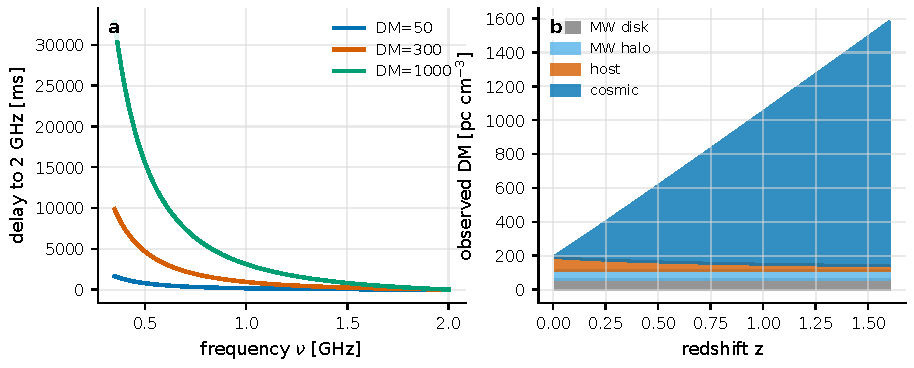
\includegraphics[width=0.94\linewidth]{figures/generated/chapter_14/ch14_dispersion_delay.pdf}
\caption{冷等离子体色散与 FRB 的色散量预算。左图把到达延迟画成频率的函数（参考频率 \(2\,{\rm GHz}\)）：低频端那条陡峭的 \(\nu^{-2}\) 曲线，就是式 \eqref{eq:e21-dispersion-delay} 让 DM 极易从宽带动态谱中读出的原因。右图把一次局域 FRB 的观测色散量拆成银河系盘、银晕、宿主星系与宇宙学等离子体四部分；宿主项因宇宙学时间膨胀按 \((1+z)^{-1}\) 进入观测值。}
\label{fig:e21-dispersion}
\end{figure}

\paragraph{色散量作为电子账本：从银河系到宇宙学}
\label{sec:e21-dmbudget}

既然 DM 是电子账本，就能反过来用它测电子。但账本必须分清是谁欠的。银河系电子密度绝非常数：NE2001 模型把厚盘、薄盘、旋臂、局部空洞和团块拼起来，用脉冲星的 DM、独立测距和散射数据约束参数；YMW16 更新了厚盘、薄盘、旋臂、银心和麦哲伦云/星系际处理，专门把一颗脉冲星或一次 FRB 的\textbf{银河系那部分 DM} 换算成距离或前景 \citep{2002astro.ph..7156C,2017ApJ...835...29Y}。高银纬视线的银河系盘贡献常为 \(30\text{--}100\,{\rm pc\,cm^{-3}}\)，银晕再添 \(50\text{--}100\,{\rm pc\,cm^{-3}}\) 量级；靠近银盘、HII 区或超新星遗迹时，局部结构会比平滑模型更重要。

对宇宙学 FRB，观测到的总色散量是一笔跨越几十亿光年的账：
\begin{equation}
  {\rm DM}_{\rm FRB}
  =
  {\rm DM}_{\rm MW,ISM}
  +{\rm DM}_{\rm MW,halo}
  +{\rm DM}_{\rm cosmic}(z)
  +\frac{{\rm DM}_{\rm host}}{1+z} .
  \label{eq:e21-frb-dm-budget}
\end{equation}
\begin{formulaexplain}
四项分别是银河系盘、银晕、沿途宇宙学等离子体、以及宿主星系的贡献。宿主项要除以 \((1+z)\)，因为宿主处发出的频率间隔和时间间隔在飞往我们的途中已经被宇宙膨胀拉伸了红移倍——同一物理延迟，在我们看来变小了。
\end{formulaexplain}
逐项的物理含义：前两项来自我们自己银河系，可以用 NE2001/YMW16 扣掉；\({\rm DM}_{\rm cosmic}(z)\) 是弥漫在星系际的重子电子，随红移单调增长，是这条式子里最值钱的一项；\({\rm DM}_{\rm host}\) 是宿主星系的贡献，最难约束。把宇宙学项写成均匀宇宙的积分：
\begin{equation}
  {\rm DM}_{\rm cosmic}(z)
  =
  \frac{3cH_0\Omega_b f_{\rm IGM}}{8\pi Gm_p}
  \int_0^z
  \frac{f_e(z')(1+z')}{\sqrt{\Omega_m(1+z')^3+\Omega_\Lambda}}
  \,{\rm d}z' .
  \label{eq:e21-cosmic-dm}
\end{equation}
\begin{formulaexplain}
\(\Omega_b,\Omega_m,\Omega_\Lambda\) 是重子、物质、暗能量密度参数，\(H_0\) 是哈勃常数，\(m_p\) 是质子质量，\(f_{\rm IGM}\) 是进入弥散星系际介质的重子比例，\(f_e\) 是每个重子提供的自由电子数。前面的系数给出平均重子密度，积分核描述膨胀宇宙里电子数密度与路径长度如何随红移变化。
\end{formulaexplain}
这条式子的分量都不神秘：系数 \(3H_0^2\Omega_b/8\pi G\) 是今天的平均重子质量密度（把临界密度乘以 \(\Omega_b\)），除以 \(m_p\) 变成数密度，再乘 \(f_e f_{\rm IGM}\) 得电子数密度；积分里的 \((1+z')\) 来自密度随膨胀的稀释被路径压缩抵消后的净因子，分母的 \(\sqrt{\Omega_m(1+z')^3+\Omega_\Lambda}\) 是 \(\Lambda\)CDM 的膨胀率 \(H(z')/H_0\)。这里有一步千万别漏：视线元不是 \({\rm d}l\) 而是随红移写的 \({\rm d}l=c\,{\rm d}z'/H(z')\)，它单独贡献一个 \(c/H_0\)（\(H_0\) 从 \(H(z')=H_0\sqrt{\cdots}\) 里提出来放进积分核的分母）。正是这个 \(c/H_0\) 和临界密度里的 \(H_0^2\) 合并，才把前因子从"\(3H_0^2\Omega_b/(8\pi G)\) 除以 \(m_p\)"的质量密度形式，凑成式中带 \(cH_0\) 的 \(3cH_0\Omega_b f_{\rm IGM}/(8\pi Gm_p)\)——比纯质量密度多一次 \(c/H_0\)。读者若自己代数，务必记得这一份来自 \({\rm d}l=c\,{\rm d}z'/H(z')\) 的 \(c/H_0\)，否则前因子会差一个因子。它的物理意义惊人地实用：\textbf{FRB 的 DM–红移关系直接称量了宇宙里的重子有多少}——这曾经是"丢失的重子"难题，如今 FRB 样本给出的这条关系已经能测量宇宙重子含量。真实的散布来自宇宙网（cosmic web）的不均匀，常写成 \(\sigma_{\rm DM}\simeq F z^{-1/2}\)，\(F\sim0.1\text{--}0.4\) 对应不同的反馈与晕气体分布 \citep{2020Natur.581..391M,2014ApJ...790..101S}。这是"污染变编码"最漂亮的一例：色散本来是挡在源前面的一层雾，结果这层雾自己称出了宇宙的重子。

\section{Faraday 旋转：给色散加上磁场的方向}
\label{sec:e21-faraday}

色散只数电子的个数，把磁场的信息丢了。如果等离子体是\textbf{磁化}的，还有第二道印记：左旋和右旋圆偏振在磁化等离子体里相速度不同，于是线偏振的振动面会随传播被旋转，且旋转角精确正比于波长平方：
\begin{equation}
  \psi(\lambda)=\psi_0+{\rm RM}\,\lambda^2 .
  \label{eq:e21-rm-angle}
\end{equation}
\begin{formulaexplain}
\(\psi\) 是观测到的线偏振角，\(\psi_0\) 是源的本征偏振角，\(\lambda\) 是波长，RM 是\textbf{旋转量}（rotation measure）。偏振角对 \(\lambda^2\) 的斜率就是 RM。所以只要在几个频率上测偏振角，画成 \(\psi\)–\(\lambda^2\) 图，斜率即得磁化等离子体的累积效应。
\end{formulaexplain}
它和色散是一对姊妹：色散给到达时间一个 \(\nu^{-2}\)（等价于 \(\lambda^2\)）的斜率，Faraday 给偏振角一个 \(\lambda^2\) 的斜率。两者都是"读斜率"。旋转量本身是电子密度与视线磁场分量的路径积分：
\begin{equation}
  {\rm RM}
  =
  0.812
  \int
  \left(\frac{n_e}{{\rm cm^{-3}}}\right)
  \left(\frac{B_\parallel}{\mu{\rm G}}\right)
  \left(\frac{{\rm d}l}{\rm pc}\right)
  \;{\rm rad\,m^{-2}} .
  \label{eq:e21-rm-definition}
\end{equation}
\begin{formulaexplain}
\(B_\parallel\) 是沿视线（指向观测者）的磁场分量，单位微高斯（\(\mu{\rm G}\)）。RM 与 DM 的关键差别：DM 的被积函数是 \(n_e\)（恒正，只会累加），RM 的被积函数是 \(n_e B_\parallel\)（带符号，磁场反向会相互抵消）。所以 RM 携带磁场的\textbf{方向}信息。
\end{formulaexplain}
把两者相除，就得到一个电子加权的视线平均磁场估计：
\begin{equation}
  \langle B_\parallel\rangle
  \simeq
  1.232\,\mu{\rm G}\;
  \frac{{\rm RM}/{\rm rad\,m^{-2}}}{{\rm DM}/{\rm pc\,cm^{-3}}}.
  \label{eq:e21-bfield-rm-dm}
\end{equation}
\begin{formulaexplain}
\(\langle B_\parallel\rangle\) 是由 RM 与 DM 之比推出的平均视线磁场。系数 \(1.232\,\mu{\rm G}\) 就是式 \eqref{eq:e21-rm-definition} 与 DM 定义里两个数值系数的比。只有当 RM 与 DM 来自\textbf{同一段介质}时，这个比值才有直接的物理含义。
\end{formulaexplain}
这不是一个"放之四海皆准"的磁场测量，用它时要盯紧两个陷阱。其一，若 RM 主要来自磁化的宿主星系、而 DM 主要来自星系际介质，两者不是同一段路，式 \eqref{eq:e21-bfield-rm-dm} 会严重低估局部磁场。其二，若视线上磁场有反向，RM 里正负抵消而 DM 不会，比值同样失真。星系团和星系际磁场的 RM 研究，常把这类简并（degeneracy）与 X 射线气体密度、射电晕、以及背景源的 RM 网格结合起来才能拆开 \citep{2002ARA&A..40..319C}。数量级上，普通星际视线的 \(|{\rm RM}|\) 多在 \(1\text{--}10^2\,{\rm rad\,m^{-2}}\)，配合 \({\rm DM}\sim30\,{\rm pc\,cm^{-3}}\)，给出 \(\langle B_\parallel\rangle\) 微高斯量级——正是银河系星际磁场的典型强度。

\begin{figure}[tbp]
\centering
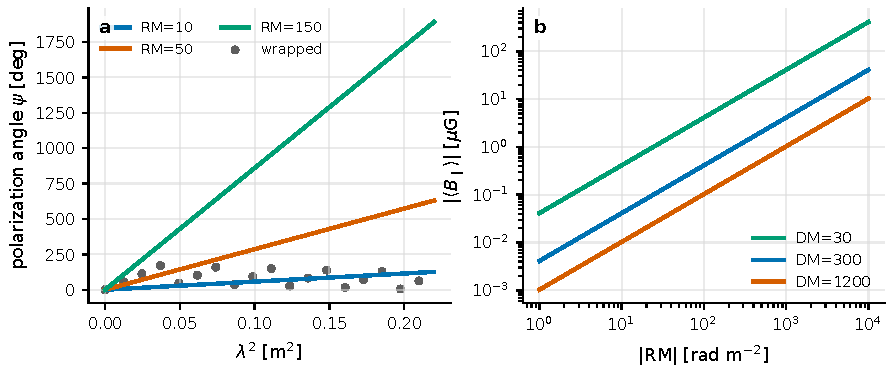
\includegraphics[width=0.94\linewidth]{figures/generated/chapter_14/ch14_faraday_rotation.pdf}
\caption{Faraday 旋转的两种读法。左图是 \(\psi=\psi_0+{\rm RM}\,\lambda^2\) 的线性关系；黑点提醒我们偏振角只能在模 \(\pi\) 意义下测得，窄带数据容易出现 \(n\pi\) 缠绕歧义（需要够宽的 \(\lambda^2\) 覆盖才能定唯一斜率）。右图把 \(\langle B_\parallel\rangle=1.232\,{\rm RM}/{\rm DM}\) 画成 RM 的函数：同一个 RM，在低 DM 的稀薄介质里代表更强的平均磁场。}
\label{fig:e21-faraday}
\end{figure}

对相干与偏振测量，Faraday 旋转的意味很直接：如果你的接收带宽跨了不小的 \(\lambda^2\) 范围，而 RM 又大，那么带宽内不同频率的偏振角被转到不同方向，把它们不加校正地平均，会\textbf{冲淡}（depolarize）净偏振——这正是第 \ref{chap:e02} 章"带宽内相位不齐会削弱相干叠加"那条精神在偏振维度上的翻版。校正的办法就是先测 RM、把每个频道的偏振角旋回本征值，再相干叠加。

\section{散射与闪烁：多路径如何搅乱相干}
\label{sec:e21-scattering}

色散和 Faraday 旋转都很"绅士"：它们只给不同频率、不同偏振加一个确定的相对延迟或旋转，去掉就还原。散射（scattering）不一样，它动的是\textbf{方向}和\textbf{相干性}本身。星际电子密度不是光滑的，湍流在各种尺度上搅出密度起伏，这些起伏像磨砂玻璃一样把平整的波前揉皱。揉皱的后果有三：源的像被角展宽（angular broadening），窄脉冲被拖出长尾（temporal broadening），强度随时间频率闪烁（scintillation）——三件事其实是同一件事在角度、时间、频率上的三个投影。

先看时间上的拖尾。波前被揉皱后，光可以走许多条稍长的路径到达我们，相当于源端一个瞬间的信号被摊到一小段时间里。在最简单的\textbf{单薄屏}（thin screen）近似下，观测脉冲是源脉冲和一个到达时间核的卷积：
\begin{equation}
  I_{\rm obs}(t)
  =
  \int I_{\rm src}(t')\,P(t-t')\,{\rm d}t',
  \qquad
  P(t)=\frac{1}{\tau_{\rm sc}}\exp\!\left(-\frac{t}{\tau_{\rm sc}}\right)H(t).
  \label{eq:e21-scattering-convolution}
\end{equation}
\begin{formulaexplain}
\(I_{\rm obs}\) 是观测强度，\(I_{\rm src}\) 是源端强度，\(P(t)\) 是散射到达时间核，\(\tau_{\rm sc}\) 是散射展宽时标，\(H(t)\) 是阶跃函数。核是\textbf{单侧}指数：光只能被绕远路而\textbf{延迟}到达，不可能提前——所以一个对称的窄脉冲，出来变成"陡升缓降"的长尾。
\end{formulaexplain}
这里 \(\tau_{\rm sc}\) 单位是秒（或毫秒），它是长尾的 \(1/e\) 衰减时间。真实视线可能有多个屏、各向异性散射、有限源尺寸，单侧指数只是最常用的低阶模型。\(\tau_{\rm sc}\) 强烈依赖频率：
\begin{equation}
  \tau_{\rm sc}\propto \nu^{-\alpha}.
  \label{eq:e21-scattering-power}
\end{equation}
\begin{formulaexplain}
\(\alpha\) 是散射的频率指数。Kolmogorov 湍流的薄屏理论给 \(\alpha\simeq4.4\)，多频脉冲星样本的经验平均更接近 \(3.9\pm0.2\)。指数这么陡，意味着往低频走，散射尾会爆炸式变长——这是低频脉冲搜索最头疼的敌人。
\end{formulaexplain}
经验上常用一条把 \(\tau_{\rm sc}\) 和 DM、频率连起来的拟合式：
\begin{equation}
  \log_{10}\!\left(\frac{\tau_{\rm sc}}{{\rm ms}}\right)
  =
  -6.46
  +0.154\log_{10}{\rm DM}
  +1.07(\log_{10}{\rm DM})^2
  -3.86\log_{10}\!\left(\frac{\nu}{\rm GHz}\right),
  \label{eq:e21-bhat-scattering}
\end{equation}
\begin{formulaexplain}
这是一条经验散射关系（DM 以 \({\rm pc\,cm^{-3}}\) 为单位），只适合做数量级预估。二次项 \((\log_{10}{\rm DM})^2\) 反映高 DM 视线穿过更多湍流；\(-3.86\log_{10}\nu\) 就是式 \eqref{eq:e21-scattering-power} 的对数版。真实视线的湍流结构会带来远超一个数量级的散布。
\end{formulaexplain}
代数字：\({\rm DM}=300\,{\rm pc\,cm^{-3}}\)、\(\nu=1.4\,{\rm GHz}\) 时它给出毫秒量级的展宽；降到 \(0.6\,{\rm GHz}\)，靠那个 \(\nu^{-3.86}\)，展宽涨到十几毫秒甚至更多。散射把毫秒脉冲拖成几十毫秒的糊团，微结构就此丢失——这是纯粹的"污染"。

现在到本章和相干性最紧要的连接。时间上的拖尾，在频率域里等价于一条\textbf{去相关带宽}（decorrelation bandwidth）\(\Delta\nu_d\)——即闪烁图样在频率上还"记得自己"的宽度：
\begin{equation}
  \tau_{\rm sc}\simeq \frac{C_1}{2\pi\,\Delta\nu_d}.
  \label{eq:e21-decorrelation-bandwidth}
\end{equation}
\begin{formulaexplain}
\(\Delta\nu_d\) 是闪烁的去相关带宽，\(C_1\) 是与几何和散射谱有关的常数（通常 \(\sim1\)）。它就是第 \ref{chap:e02} 章"时间宽度与谱宽度成反比"那条测不准关系的散射版：多路径延迟越长（\(\tau_{\rm sc}\) 大），频率上相关带宽 \(\Delta\nu_d\) 越窄。
\end{formulaexplain}
这条式子把散射对相干测量的意义讲透了。回忆第 \ref{chap:e02} 章：相干时间 \(\tau_c\simeq1/\Delta\nu\)。散射相当于给信号叠了一个额外的、随机的相位结构，它的"相干带宽"就是 \(\Delta\nu_d\)。当散射很强，\(\Delta\nu_d\) 窄得只有几十 kHz，你在一个几百 MHz 的宽带里做相干叠加，等于把几千个互不相干的斑块硬加起来——净相干度被冲淡到几乎为零。反过来，散射也\textbf{编码}信息：当散射较弱、\(\Delta\nu_d\) 可测时，闪烁斑随时间频率的漂移能反解出散射屏的速度、屏到我们的距离、乃至源的角尺寸——一台"星际闪烁望远镜"，其等效角分辨率可达微角秒，远超任何单口径望远镜。这就是散射的两副面孔：既是抹平相干的磨砂玻璃，又是免费的超高分辨探针。

\begin{figure}[tbp]
\centering
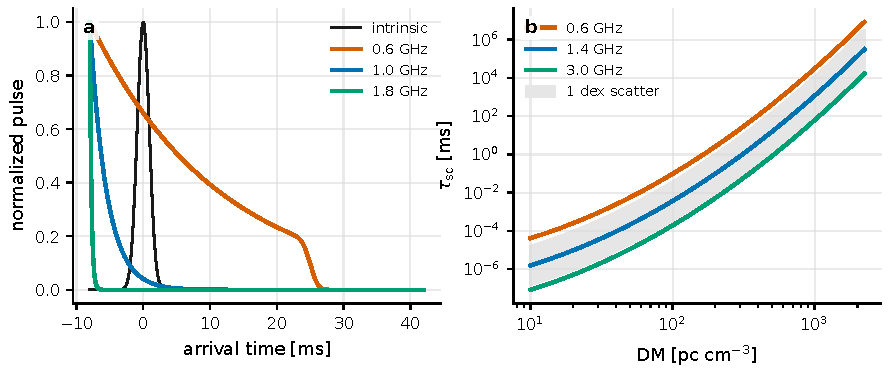
\includegraphics[width=0.94\linewidth]{figures/generated/chapter_14/ch14_scattering_broadening.pdf}
\caption{星际散射把短脉冲拖成带长尾的到达时间分布。左图把一个窄高斯脉冲与单侧指数核卷积；频率越低，\(\tau_{\rm sc}\propto\nu^{-4}\) 把尾巴拉得越长，脉冲的对称性被彻底破坏。右图用经验关系画出 \(\tau_{\rm sc}\) 随 DM 与频率的变化，灰带表示固定 DM 下常见的一个数量级以上的散布。}
\label{fig:e21-scattering}
\end{figure}

顺带一提：等离子体不只会"揉皱"波前，横向的电子柱密度梯度还能像一枚（频率相关的）透镜那样\textbf{折射}光线，低频偏折更强，可造成窄带的放大、焦散甚至多像。这提醒我们，即便把 \(\nu^{-2}\) 色散去干净了，动态谱里残留的结构也可能仍是传播的产物，而非源的本征变化 \citep{1998ApJ...496..253C,2014MNRAS.437.2180E}。在银心方向做毫米波 VLBI 时，这道强散射屏尤其麻烦：给 Sgr A* 的事件视界尺度成像，必须同时处理本征结构、散射模糊和时间变化 \citep{2008Natur.455...78D,2022ApJ...930L..14E,2022ApJ...930L..15E}。

\section{尘埃：一条带波长选择的损耗通道}
\label{sec:e21-dust}

等离子体主要动射电和到达时间；尘埃（dust）主要动光学、红外的\textbf{通量与颜色}。对光学光子，尘埃颗粒像一条挑肥拣瘦的损耗通道：它按波长选择性地吸收和散射，短波（蓝光）损失得比长波（红光）多，于是穿过尘埃的星光既变暗又变红。最基本的消光关系是
\begin{equation}
  F_{\lambda,{\rm obs}}
  =
  F_{\lambda,{\rm int}}\,10^{-0.4A_\lambda},
  \label{eq:e21-extinction-flux}
\end{equation}
\begin{formulaexplain}
\(F_{\lambda,{\rm int}}\) 是本征通量，\(F_{\lambda,{\rm obs}}\) 是消光后的通量，\(A_\lambda\) 是波长 \(\lambda\) 处的消光，单位星等（mag）。星等本就是对数标度，所以 \(A_\lambda\) 在指数上以 \(10^{-0.4A_\lambda}\) 的形式压低通量：\(A_\lambda=1\) 星等对应通量降到约 \(0.40\) 倍，\(A_\lambda=2.5\) 对应降到约 \(0.10\) 倍。
\end{formulaexplain}
消光随波长的变化，用两个量来概括其"红化"程度：
\begin{equation}
  E(B-V)=A_B-A_V,
  \qquad
  R_V=\frac{A_V}{E(B-V)}.
  \label{eq:e21-rv-definition}
\end{equation}
\begin{formulaexplain}
\(E(B-V)\) 是蓝波段 \(B\) 与可见波段 \(V\) 消光之差，叫\textbf{色余}（color excess），度量星光被"染红"了多少；\(R_V=A_V/E(B-V)\) 是总消光对选择性红化之比，度量消光曲线的"灰度"。\(R_V\) 越大，曲线越平（越灰），说明较大的尘埃颗粒占主导。
\end{formulaexplain}
逐项落地：\(A_B,A_V\) 是 \(B\)、\(V\) 波段的消光（各以 mag 计），\(E(B-V)\) 单位也是 mag。银河系平均 \(R_V\simeq3.1\)，弥散星际介质多在 \(2.5\text{--}3.5\)，致密分子云里可到 \(5\) 以上（大颗粒使消光更灰）。Cardelli–Clayton–Mathis（CCM）消光律把红外、光学、紫外的平均曲线压缩成一个由 \(R_V\) 参数化的单参数族；Fitzpatrick 进一步指出真实视线仍有明显散布，尤其在 \(2175\,\text{\AA}\) 的紫外驼峰（UV bump）和远紫外上翘的强弱上 \citep{1989ApJ...345..245C,1999PASP..111...63F,2003ARA&A..41..241D}。

这里有一个对瞬变和偏振测量至关重要的\textbf{误差地板}。若你只用一条平均消光律去改正一个 \(E(B-V)=0.2\) 星等的蓝色源，紫外端残留 \(0.1\) 星等的误差毫不稀奇——对偏振角、颜色温度、以及瞬变源早期的谱能量分布（SED），这就是主导性的系统误差。换句话说，尘埃不仅让源变暗，它还给"颜色"这个测量注入了不可忽视的不确定度。

尘埃颗粒多是非球形的，它们在星际磁场里会部分排列取向，于是对不同振动方向的星光吸收不等，给穿过的星光注入一点\textbf{线偏振}。其波长依赖用经验的 Serkowski 关系描述：
\begin{equation}
  \frac{P(\lambda)}{P_{\max}}
  =
  \exp\!\left[-K\ln^2\!\left(\frac{\lambda_{\max}}{\lambda}\right)\right].
  \label{eq:e21-serkowski}
\end{equation}
\begin{formulaexplain}
\(P(\lambda)\) 是尘埃造成的线偏振度，\(P_{\max}\) 是峰值偏振，\(\lambda_{\max}\) 是峰值波长，\(K\) 控制曲线宽度。它是一条以 \(\ln(\lambda_{\max}/\lambda)\) 为变量的高斯型峰：偏振在 \(\lambda_{\max}\) 处最大，向两侧对称衰减。峰的位置 \(\lambda_{\max}\) 对颗粒尺寸敏感。
\end{formulaexplain}
经验上 \(\lambda_{\max}\approx0.55\,\mu{\rm m}\)，峰值偏振度的上限约为 \(P_{\max}\lesssim9\,E(B-V)\%\)（即每 0.1 mag 色余最多约 0.9\% 偏振）。这个上限并非每条视线都能达到，它受颗粒形状、取向效率、视线上磁场方向的变化、以及多层云叠加影响 \citep{1975ApJ...196..261S,2015ARA&A..53..501A}。对任何想测源本征偏振的实验，这条尘埃偏振是必须先扣掉的前景。

尘埃还能把一次短暂的爆发"回放"成\textbf{光回声}（light echo）或 X 射线晕：爆发的光被途中尘埃散射进我们的视线，因为绕了个弯，比直达光晚到。若尘埃屏位于源到观测者距离的比例 \(x\) 处、散射角为 \(\theta\)，几何延迟近似为
\begin{equation}
  \Delta t_{\rm dust}
  \simeq
  \frac{D_s}{2c}\,\frac{x}{1-x}\,\theta^2 .
  \label{eq:e21-dust-delay}
\end{equation}
\begin{formulaexplain}
\(\Delta t_{\rm dust}\) 是尘埃散射的几何延迟，\(D_s\) 是源距离，\(x\) 是尘埃屏的相对位置（\(0\) 在源、\(1\) 在观测者），\(\theta\) 是散射角。延迟正比于 \(\theta^2\)，所以角分辨的光回声能反推尘埃的几何位置——延迟随散射角的展开，就是一把测距的尺。
\end{formulaexplain}
数量级上，对银河系源，角秒级散射角给出小时到天的延迟；对河外源，尘埃的几何位置和望远镜角分辨要一起进入模型。这又是一次"污染即编码"：本来是挡光的尘埃，借着延迟–角度关系，成了测量爆发周围三维尘埃分布的探针。

\begin{figure}[tbp]
\centering
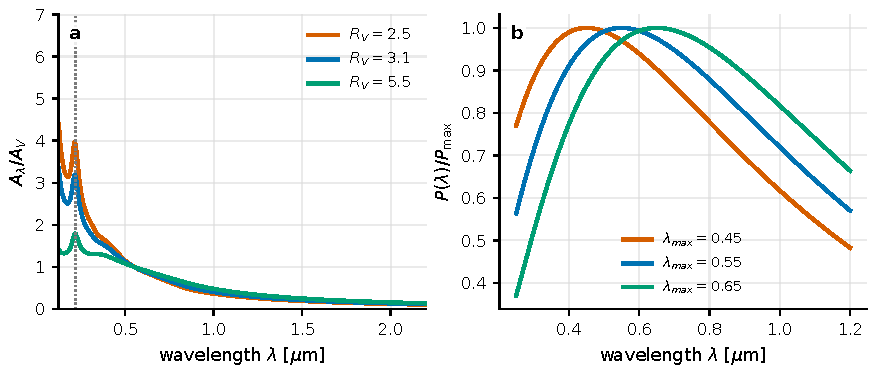
\includegraphics[width=0.94\linewidth]{figures/generated/chapter_14/ch14_dust_extinction_polarization.pdf}
\caption{尘埃同时改变光子的通量、颜色与偏振。左图是 CCM 平均消光曲线，\(R_V\) 越大、光学到近红外越"灰"；\(0.2175\,\mu{\rm m}\) 附近的紫外驼峰是小颗粒和碳质材料的重要诊断。右图是 Serkowski 偏振曲线，峰位 \(\lambda_{\max}\) 的移动反映颗粒尺寸与取向环境的变化。}
\label{fig:e21-dust}
\end{figure}

\section{引力透镜：把一条路径变成多条}
\label{sec:e21-lensing}

前面三位改写者都来自真实的介质——电子、磁场、尘埃颗粒。最后一位不一样：引力透镜（gravitational lensing）来自\textbf{弯曲的时空}本身。它不改变光子的频率（不色散），却改变光走的路径、方向和到达时间。对事件表来说，透镜的核心动作可以用一句话概括：\textbf{一个源事件，可以变成多个像、多个到达时刻、多个放大权重}。

在薄透镜近似下，源的真实方向和我们看到的像方向由透镜方程连接：
\begin{equation}
  {\boldsymbol\beta}
  =
  {\boldsymbol\theta}
  -
  {\boldsymbol\alpha}({\boldsymbol\theta}),
  \label{eq:e21-lens-equation}
\end{equation}
\begin{formulaexplain}
\({\boldsymbol\beta}\) 是源的真实角位置，\({\boldsymbol\theta}\) 是像的角位置，\({\boldsymbol\alpha}\) 是约化偏折角（reduced deflection angle），都以角度（rad 或 arcsec）计。方程说：我们看到的像方向 \({\boldsymbol\theta}\)，等于真实方向 \({\boldsymbol\beta}\) 加上质量把光线扳过来的角度。给定 \({\boldsymbol\beta}\)，这个方程可以有\textbf{多个} \({\boldsymbol\theta}\) 解——那就是多重像。
\end{formulaexplain}
偏折的自然角尺度由 Einstein 角给出。对一个点质量透镜，
\begin{equation}
  \theta_E
  =
  \left(
  \frac{4GM}{c^2}
  \frac{D_{ls}}{D_lD_s}
  \right)^{1/2}.
  \label{eq:e21-einstein-angle}
\end{equation}
\begin{formulaexplain}
\(\theta_E\) 是 Einstein 角，\(M\) 是透镜质量，\(G\) 是引力常数，\(D_l,D_s,D_{ls}\) 分别是观测者到透镜、到源、以及透镜到源的角直径距离。核心因子 \(4GM/c^2\) 就是广义相对论光线偏折的招牌（是牛顿预言的两倍）。\(\theta_E\) 定下多重像分离与微透镜的天然尺度。
\end{formulaexplain}
两个真实数量级把两种透镜分开。\(M=1\,M_\odot\)、银河系尺度几何，给出毫角秒（mas）量级的 \(\theta_E\)——这么小分不开两个像，只能看到亮度随时间起伏，这就是\textbf{微透镜}（microlensing）：一颗前景恒星飘过背景星前面，把它短暂放大。而 \(M\sim10^{11}\text{--}10^{12}\,M_\odot\) 的星系透镜，给出角秒（arcsec）量级的 \(\theta_E\)，多重像清清楚楚分得开，这是\textbf{强透镜}（strong lensing）。放大率由像面到源面的映射的雅可比行列式决定：
\begin{equation}
  \mu
  =
  \frac{1}{\det\!\left(\partial{\boldsymbol\beta}/\partial{\boldsymbol\theta}\right)}.
  \label{eq:e21-magnification}
\end{equation}
\begin{formulaexplain}
\(\mu\) 是放大率，分母是从像平面 \({\boldsymbol\theta}\) 到源平面 \({\boldsymbol\beta}\) 的雅可比行列式。透镜不产生也不吸收光子，只是重新分配立体角，所以面积被拉伸多少倍，亮度就放大多少倍。当行列式趋于零，像面被无限拉伸，放大率发散——那条曲线叫焦散（caustic）。
\end{formulaexplain}
焦散附近 \(|\mu|\) 可以非常大（理论上发散），但有限的源尺寸、微透镜、尘埃和时间采样都会把实际能观测到的峰值放大压下来。这条式子的物理很干净：放大是几何的重新分配，不是能量的凭空增加。

现在到透镜最深刻、也最贴合本书主线的一点：\textbf{时间延迟}。不同的像走的是不同长度、且穿过不同深浅引力势的路径，所以它们的光不是同时到达的。到达时间由 Fermat 势（Fermat potential）控制：
\begin{equation}
  t({\boldsymbol\theta},{\boldsymbol\beta})
  =
  \frac{D_{\Delta t}}{c}
  \left[
  \frac{1}{2}\,|{\boldsymbol\theta}-{\boldsymbol\beta}|^2
  -
  \psi({\boldsymbol\theta})
  \right],
  \qquad
  D_{\Delta t}
  =
  (1+z_l)\frac{D_lD_s}{D_{ls}} .
  \label{eq:e21-fermat-delay}
\end{equation}
\begin{formulaexplain}
\(t\) 是相对到达时间，方括号里第一项 \(\tfrac12|{\boldsymbol\theta}-{\boldsymbol\beta}|^2\) 是\textbf{几何路径差}（绕远路多花的时间），第二项 \(\psi\) 是\textbf{引力势延迟}（Shapiro 延迟，光在深势阱里"走得慢"）。\(D_{\Delta t}\) 是时间延迟距离，\(z_l\) 是透镜红移。真实的像出现在这个时间面的\textbf{驻点}（极小、极大或鞍点）——这正是费马原理："光走极值时间的路"。
\end{formulaexplain}
时间延迟的几何起源就藏在这两项的拉锯里：偏离源方向越远，几何项越大（迟到），但通常也越靠近质量、势阱越深（Shapiro 项也在变）。两幅像的观测延迟，就是它们 Fermat 势之差：
\begin{equation}
  \Delta t_{AB}
  =
  \frac{D_{\Delta t}}{c}\,
  \Delta\phi_{AB}.
  \label{eq:e21-time-delay-distance}
\end{equation}
\begin{formulaexplain}
\(\Delta t_{AB}\) 是像 \(A\) 与像 \(B\) 的到达时差，\(\Delta\phi_{AB}\) 是二者的 Fermat 势差（由透镜质量模型算出）。测出 \(\Delta t_{AB}\)、再有一个透镜模型给出 \(\Delta\phi_{AB}\)，就能反解出 \(D_{\Delta t}\)——而 \(D_{\Delta t}\propto 1/H_0\)，于是时间延迟直接测量了哈勃常数。
\end{formulaexplain}
数量级：星系强透镜的 \(\Delta t_{AB}\) 常为天到月，少数可达年。注意它只占 \(D_{\Delta t}/c\) 的约 \(10^{-11}\)（因为 \(\Delta\phi_{AB}\) 是个小数），所以透镜势、外部收敛（external convergence）、质量片简并（mass-sheet degeneracy）和光变曲线采样的每一点误差，都会直接灌进 \(H_0\) 的误差预算。Refsdal 早在 1964 年就指出多重像时间延迟可以测 \(H_0\)；现代的时间延迟宇宙学（time-delay cosmography）靠多年监测、高分辨成像、透镜星系速度弥散和环境建模，把这条思路做成了独立于宇宙微波背景的 \(H_0\) 测量 \citep{1964MNRAS.128..295R,1964MNRAS.128..307R,1986ApJ...310..568B,2016A&ARv..24...11T}。这是本章的又一记漂亮编码：时间延迟本是"同一个源被复制出好几个错时副本"的污染，结果这错时里锁着宇宙的膨胀率。

\begin{figure}[tbp]
\centering
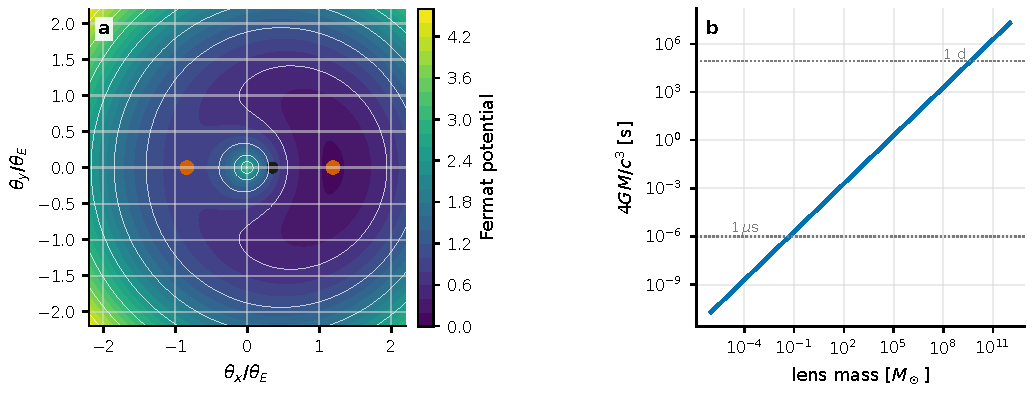
\includegraphics[width=0.94\linewidth]{figures/generated/chapter_14/ch14_lensing_time_delay.pdf}
\caption{强透镜的两个尺度。左图是点质量透镜的 Fermat 到达时间面，黑点是源位置，两个橙点是像位置；像恰好出现在到达时间面的驻点（极小与鞍点）。右图给出基本延迟尺度 \(4GM/c^3\)：恒星质量透镜落在微秒到毫秒，星系与星系团透镜自然进入天到年的时间域。}
\label{fig:e21-lensing}
\end{figure}

\paragraph{当波长不能忽略：从光线到衍射}
\label{sec:e21-wavelensing}

前面把光当成"光线"，默认多条路径可以清清楚楚分开。但当波长和透镜引起的时间延迟相当时，几何光学失效，必须回到\textbf{波}的图像——就像第 \ref{chap:e02} 章反复强调的，波会衍射、会干涉。判据是一个无量纲频率：
\begin{equation}
  w
  =
  \frac{8\pi GM(1+z_l)f}{c^3}.
  \label{eq:e21-wave-lensing-w}
\end{equation}
\begin{formulaexplain}
\(w\) 是波动透镜的无量纲频率，\(M\) 是透镜质量，\(f\) 是波的频率，\(z_l\) 是透镜红移。\(w\) 比较的是波的周期 \(1/f\) 与透镜引起的时间延迟尺度 \(\sim GM/c^3\)：\(w\gg1\) 时延迟远长于周期，回到几何光学；\(w\lesssim1\) 时延迟不到一个周期，衍射不可忽略。
\end{formulaexplain}
在几何区（\(w\gg1\)），多重像可以分开，并像双缝一样相干干涉；在衍射区（\(w\lesssim1\)），焦散被抹平，放大率不再能简单地把几何像相加。频域波形写成
\begin{equation}
  \tilde h_L(f)=F(f)\,\tilde h(f),
  \label{eq:e21-wave-amplification}
\end{equation}
\begin{formulaexplain}
\(\tilde h(f)\) 是未透镜的频域波形，\(\tilde h_L(f)\) 是透镜后的，\(F(f)\) 是复放大因子（complex amplification factor）。它是复数，所以同时携带\textbf{振幅放大}（模）和\textbf{相位延迟}（辐角），能造出频率依赖的干涉花纹。
\end{formulaexplain}
若两条路径延迟为 \(\Delta t\)，两路复振幅相加，随频率的拍频给出频域条纹间隔
\begin{equation}
  \Delta f \simeq \frac{1}{\Delta t}.
  \label{eq:e21-lensing-fringe-spacing}
\end{equation}
\begin{formulaexplain}
\(\Delta f\) 是频域干涉条纹的间距，\(\Delta t\) 是两条路径的时间延迟。这正是傅里叶那条老规矩（第 \ref{chap:e02} 章）的又一次现身：时间上相隔 \(\Delta t\) 的两个副本，在频谱上织出间距 \(1/\Delta t\) 的条纹。路径延迟越长，频域振荡越密。
\end{formulaexplain}
代数字：\(\Delta t=2\,{\rm ms}\) 给出 \(\Delta f\approx500\,{\rm Hz}\) 的条纹间隔。对光学、射电的电磁波频率 \(f\sim10^{14}\) 或 \(10^{9}\,{\rm Hz}\)，普通恒星或星系质量透镜的 \(w\) 大得惊人，几何光学好得几乎完美；但对 LISA 频段的引力波（\(f\sim10^{-3}\,{\rm Hz}\)）配上 \(10^{6}\text{--}10^{9}\,M_\odot\) 的透镜，\(w\sim1\) 的波动光学效应会真的落进观测带 \citep{2003ApJ...595.1039T}。这是透镜与本书量子光学主线最直接的接口：透镜后的干涉，本质上是同一个源场沿两条路径的相干叠加，读的还是相位。

\begin{figure}[tbp]
\centering
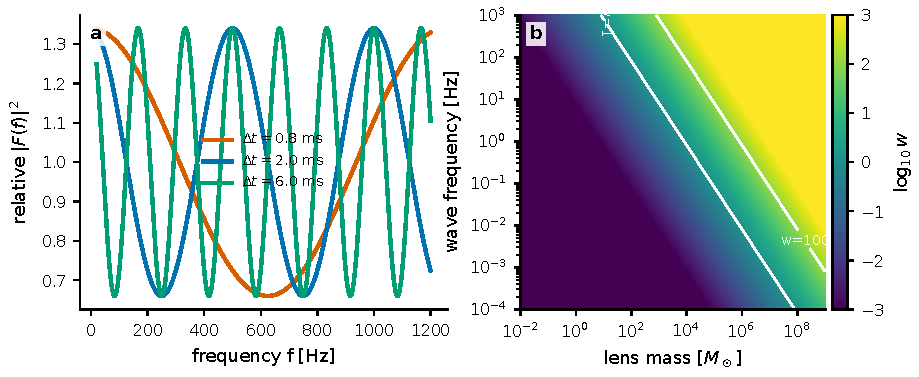
\includegraphics[width=0.94\linewidth]{figures/generated/chapter_14/ch14_wave_lensing_interference.pdf}
\caption{波动光学透镜把时间延迟转写成频域条纹。左图画出不同路径延迟下相对放大因子的振荡，条纹间距 \(\Delta f\simeq1/\Delta t\)。右图给出 \(w=8\pi GMf/c^3\) 的量级；白线 \(w=1\) 附近是衍射与几何光学的过渡，\(w\gtrsim100\) 时通常可把各像当成独立路径处理。}
\label{fig:e21-wave-lensing}
\end{figure}

\section{污染还是编码：传播对相干与计时的意义}
\label{sec:e21-correlation}

绕了一圈，回到本书的主线——相关函数。前面几节都在改写\textbf{单个事件的标签}，这一节要看它们如何改写\textbf{事件之间的相关}。核心洞见很简单：多路径传播（散射、透镜）会重排强度相关，因为观测到的两次涨落，未必来自源端同一时刻——它们可能是源端同一个结构沿不同路径、错时到达的两个副本。

把可分辨的多路径写成一串 delta 脉冲响应：
\begin{equation}
  h(t)=\sum_i \sqrt{\mu_i}\,e^{i\varphi_i}\,\delta(t-t_i),
  \label{eq:e21-multipath-impulse}
\end{equation}
\begin{formulaexplain}
\(h(t)\) 是多路径脉冲响应，\(\mu_i\) 是第 \(i\) 条路径的放大率，\(\varphi_i\) 是它的相位，\(t_i\) 是它的到达延迟。每个 delta 函数就是一条可分辨的路径——它是式 \eqref{eq:e21-channel-time} 那个抽象 \(h_{ij}\) 在"离散多像"情形下的具体样子。
\end{formulaexplain}
如果相位 \(\varphi_i\) 在观测带宽或源尺寸上被平均掉（相干被冲淡时的常见情形），观测强度就是各路径强度按放大率加权、错时叠加：
\begin{equation}
  I_{\rm obs}(t)
  =
  \sum_i \mu_i\,I_{\rm src}(t-t_i).
  \label{eq:e21-multipath-intensity}
\end{equation}
\begin{formulaexplain}
\(I_{\rm obs}\) 是观测强度，\(I_{\rm src}\) 是源端强度。相位平均后，干涉项消失，只剩各路径的强度按 \(\mu_i\) 加权相加——所以源端的一次变化，会在几个不同延迟 \(t_i\) 处各重复一遍。
\end{formulaexplain}
对强度涨落 \(\delta I=I-\langle I\rangle\) 做自相关，就能看到"回声"如何进入相关函数：
\begin{equation}
  C_{\rm obs}(\tau)
  =
  \left\langle
  \delta I_{\rm obs}(t)\,
  \delta I_{\rm obs}(t+\tau)
  \right\rangle
  =
  \sum_{ij}\mu_i\mu_j\,
  C_{\rm src}\!\left(\tau+t_i-t_j\right).
  \label{eq:e21-correlation-echo}
\end{equation}
\begin{formulaexplain}
\(C_{\rm obs}\) 是观测强度自相关，\(C_{\rm src}\) 是源端自相关。双重求和意味着\textbf{每一对路径}都贡献一个相关回声，回声出现在 \(\tau=t_j-t_i\) 处，权重是 \(\mu_i\mu_j\)。原本一个峰，被复制成一梳子的回声峰。
\end{formulaexplain}
这条式子把传播对第 \ref{chap:e08} 章那套强度相关工具的影响说清楚了：\textbf{相关峰不再唯一对应源端物理}。热光的 \(g^{(2)}(0)\) 峰、脉冲星巨脉冲的微结构、FRB 的窄带闪烁、透镜多像的延迟，都能落进这个框架，但它们的相干时间、带宽和统计分布各不相同——光看到一个相关峰，还不足以断定它的物理来源。用式 \eqref{eq:e21-correlation-echo} 时的前提很硬：源本身要有可测的快结构、传播路径要稳定、观测时间要够长、背景与选择函数要建过模。这正是把传播当成"有记忆通道"这个视角的回报——它逼你在解读任何相关峰之前，先问一句"这会不会只是一条晚到的路径？"

传播效应还划定了一类量子基础实验的边界。所谓宇宙 Bell 检验（cosmic Bell test），用纠缠光子对在两个站点做测量，两边各选测量设置 \(a,a'\) 和 \(b,b'\)，构造 CHSH 组合：
\begin{equation}
  S
  =
  E(a,b)+E(a,b')+E(a',b)-E(a',b'),
  \qquad
  |S|\le 2 .
  \label{eq:e21-chsh}
\end{equation}
\begin{formulaexplain}
\(S\) 是 CHSH 组合，\(E(a,b)\) 是给定设置下两站测量结果的相关期望值。局域隐变量理论要求 \(|S|\le2\)；量子力学可以违反到 \(2\sqrt2\)。宇宙 Bell 实验的独到之处，是用\textbf{天文光子}实时决定设置 \(a,b\)。
\end{formulaexplain}
它的用意不是说天体光子本身处于纠缠态，而是拿遥远天体的光子来\textbf{实时选择}测量设置：银河系恒星版本用星光颜色产生 \(a,b\)，把可能的"共同原因"推到几百到几千年前；类星体版本更狠，把自由选择漏洞的共同过去推到宇宙早期 \citep{2017PhRvL.118f0401H,2018PhRvL.121h0403R}（图 \ref{fig:e21-cosmic-bell}）。而这正需要本章全部内容：星光的到达时间要扣掉大气延迟（第 \ref{chap:e13} 章的时间同步），颜色要扣掉尘埃红化，射电类星体还要考虑色散和散射，仪器电子延迟要逐项进入实验时序——传播中的每一项吸收、红化、色散、延迟，都必须放进实验的因果时序里，否则漏洞就补不严。

\begin{figure}[tbp]
\centering
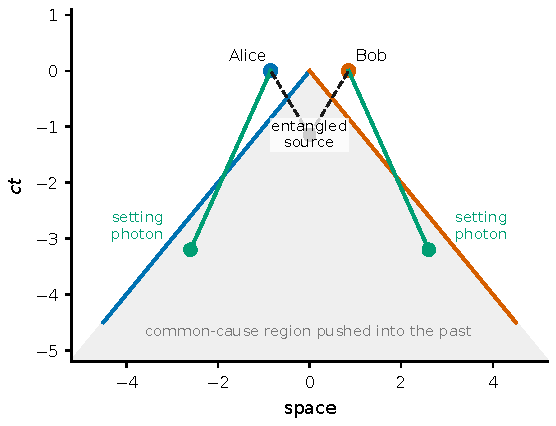
\includegraphics[width=0.72\linewidth]{figures/generated/chapter_14/ch14_cosmic_bell_lightcones.pdf}
\caption{宇宙 Bell 实验的光锥结构。纠缠源在本地实验中发出光子对，Alice 与 Bob 的测量设置由远处恒星或类星体的光子实时决定；这些设置光子的发射事件越早、方向分离越大，能被排除掉"共同原因"的时空区域就越大（图中灰区）。真实实验还要逐项加入大气传播、尘埃红化、探测器响应与电子延迟——这正是本章各效应必须进入实验时序的地方。}
\label{fig:e21-cosmic-bell}
\end{figure}

最后，把这些"平常的"传播效应看成新物理搜索的\textbf{误差地板}。类轴子粒子（axion-like particle）可以让光子在磁场里转化而造成谱吸收，宇宙双折射会旋转偏振，暗物质小结构能改写透镜的放大率和时间延迟——这些迷人的解释，都必须先和等离子体色散、尘埃、常规透镜、仪器项放在同一个模型里比较。只有当一个残余信号同时经得起时间、频率、偏振、角位置四道检验、且已知传播效应都扣不掉它时，它才有资格排队当新物理的候选。这就是"污染即背景，编码即信号"这条本章主旨最实用的收尾：先把这条有记忆的通道刻画到底，剩下的才是真正属于源、乃至属于新物理的东西。

\section*{本章要点}
\addcontentsline{toc}{section}{本章要点}

\begin{itemize}
\item \textbf{传播是有记忆的通道，不是灰玻璃。} 式 \eqref{eq:e21-channel-time} 把源端场到探测器事件写成卷积：介质重写每个光子的时间、频率、偏振、方向标签，而不只是乘一个常数。
\item \textbf{色散的 \(\nu^{-2}\) 定律是从群速度一步步推出来的。} 折射率 \(\to\) 群速度 \(v_g\approx c(1-\omega_p^2/2\omega^2)\) \(\to\) 沿视线积分，得到 \(\Delta t\propto{\rm DM}/\nu^2\)（式 \eqref{eq:e21-dm-delay}）。低频迟到的根源就是"低频群速度更慢"。DM 是电子柱密度，FRB 的 DM–红移关系能称量宇宙重子。
\item \textbf{Faraday 旋转给色散补上磁场方向。} 偏振角对 \(\lambda^2\) 的斜率是 RM，它的被积函数 \(n_e B_\parallel\) 带符号，故 RM/DM 给出电子加权平均磁场（式 \eqref{eq:e21-bfield-rm-dm}），但仅当二者同源才有直接物理含义。
\item \textbf{散射搅乱相干，也免费提供超高分辨。} 单侧指数核把窄脉冲拖成长尾（\(\tau_{\rm sc}\propto\nu^{-4}\)），去相关带宽 \(\Delta\nu_d\simeq1/2\pi\tau_{\rm sc}\)（式 \eqref{eq:e21-decorrelation-bandwidth}）决定宽带相干叠加会不会被冲淡；弱散射时闪烁反能反解屏速度、屏距离与源角尺寸。
\item \textbf{尘埃是带波长选择的损耗通道。} 消光 \(F_{\rm obs}=F_{\rm int}10^{-0.4A_\lambda}\) 让源既暗又红，\(R_V\) 定曲线灰度；平均消光律的残差是偏振与早期 SED 的主导系统误差；Serkowski 偏振和尘埃光回声都是必须先扣的前景。
\item \textbf{引力透镜把一条路径变成多条。} Einstein 角定尺度（恒星质量 mas，星系 arcsec），放大率是几何雅可比的倒数，时间延迟由 Fermat 势的几何项加 Shapiro 项决定（式 \eqref{eq:e21-fermat-delay}），并因 \(D_{\Delta t}\propto1/H_0\) 而测量哈勃常数。波长不可忽略时用无量纲频率 \(w\) 判几何/衍射区。
\item \textbf{污染即编码。} 多路径把源端一次涨落复制成相关回声（式 \eqref{eq:e21-correlation-echo}），所以相关峰不唯一对应源端物理；这些常规效应又构成宇宙 Bell 检验的时序约束与新物理搜索的误差地板。
\end{itemize}

\medskip
\noindent\textbf{想一想。}
\begin{itemize}
\item 若某 FRB 在 \(1.4\,{\rm GHz}\) 和 \(0.8\,{\rm GHz}\) 之间测得 \(1.2\,{\rm s}\) 的延迟，它的 DM 约是多少？（用式 \eqref{eq:e21-dispersion-delay} 反解。）这条视线若主要在银河系内，对照高银纬典型值合理吗？
\item 同样一个 RM，如果视线上存在一次磁场反向，你测到的 RM 会偏大还是偏小？为什么 DM 不受这个反向影响？
\item 一个星系强透镜的两幅像时间延迟测得 \(30\) 天，透镜模型给出 \(\Delta\phi_{AB}\)。要把 \(H_0\) 测到 3\% 精度，式 \eqref{eq:e21-time-delay-distance} 里哪些环节（光变采样、外部收敛、质量片简并）最可能成为瓶颈？
\end{itemize}

\chapter{暗物质、轴子与偏振量子通道}
\label{chap:e22}

\begin{chapteropening}
上一章（第 \ref{chap:e21} 章）我们把光一路飞来所受的传播改写全记了账：磁化等离子体让偏振面随 \(\lambda^2\) 拧转（法拉第旋转），引力透镜把像复制、移位、拉伸。请把那一章的结论记牢——那些等离子体前景和透镜通道，正是本章要找的新物理必须先甄别、再撬开的\emph{对照组}。而更早在第 \ref{chap:e18} 章我们还在磁星表面看到一件奇事：磁场强到接近临界场时，\emph{真空本身}都变成了一种有偏振方向的介质。那时留下一句话——偏振（polarization）是一条独立的量子通道，值得单独打开。这一章就来兑现它。新物理很少送给我们一张干净的"新粒子照片"；它更喜欢藏在偏振角的一次微小拧转里、藏在偏振随时间的缓慢摆动里、藏在强磁场里某个能段异常增亮的光子里。这一章的主角是轴子（axion）和轴子样粒子（axion-like particle，ALP）：它们通过一个极简单的耦合 \(a\,\bm E\cdot\bm B\) 与光对话，能让线偏振面转过一个角度，能让偏振信号随暗物质场一起振荡，还能在中子星、磁星和黑洞的强场环境里把一部分光"变"成或"变"走。我们的任务分三步：先把这个耦合翻译成一个能观测的旋转角，把它随耦合常数和传播路径的关系一步步写出来；再看看怎样用\emph{偏振分辨的强度与相干测量}去抓这个微弱到 \(10^{-3}\) 弧度甚至更小的信号；最后把它放回致密天体的强场里，问一句最要命的话——这到底是新物理，还是仪器和前景在骗我们？
\end{chapteropening}


\section{一个耦合，两个观测量：旋转与转换}
\label{sec:e22-coupling}

先把态度摆正：这一章不急着宣布"发现了轴子"。我们的做法始终是——先把"新物理"翻译成一个具体的观测量，再反过来问，普通天体物理和普通仪器能不能\emph{伪造}出同一个观测量。对轴子来说，最干净的两个入口都来自\emph{同一个}相互作用项：一个是线偏振面被轻轻拧转（旋转，rotation），另一个是在外磁场里轴子和光子互相变身（转换，conversion）。

在低能有效理论里，轴子样场 \(a\) 与电磁场的耦合写成

\begin{equation}
  \mathcal L_{a\gamma}
  = -\frac{1}{4}\,g_{a\gamma}\,a\,F_{\mu\nu}\tilde F^{\mu\nu}
  = g_{a\gamma}\,a\,\bm E\cdot\bm B .
  \label{eq:e22-lagrangian}
\end{equation}
\begin{formulaexplain}
\(a\)：轴子样场（能量量纲）；\(g_{a\gamma}\)：轴子--光子耦合常数，量纲 \(\mathrm{energy^{-1}}\)，天体文献惯用 \(\mathrm{GeV^{-1}}\)；\(F_{\mu\nu}\)、\(\tilde F^{\mu\nu}\)：电磁张量与它的对偶。写成 \(\bm E\cdot\bm B\) 后一眼看出：只有当电场、磁场取向"手性"相关时，这一项才起作用。
\end{formulaexplain}

把每个符号落到地上。\(F_{\mu\nu}\) 就是我们熟悉的电磁场张量，它的对偶 \(\tilde F^{\mu\nu}=\tfrac12\epsilon^{\mu\nu\alpha\beta}F_{\alpha\beta}\) 把电场和磁场对调了位置，所以 \(F\tilde F\propto \bm E\cdot\bm B\) 是一个赝标量（parity-odd）——它在空间反射下变号。轴子 \(a\) 也是赝标量，两者相乘才凑成一个真正的标量，才能进拉氏量。耦合常数 \(g_{a\gamma}\) 的大小是我们要测的靶心：天体和实验室的现有限制普遍把它压在 \(10^{-10}\text{--}10^{-12}\,\mathrm{GeV^{-1}}\) 这个量级以下。对严格的 QCD 轴子（QCD axion），质量与破缺尺度还锁在一条窄带上，

\begin{equation}
  m_a \simeq 5.7\,\mu\mathrm{eV}\left(\frac{10^{12}\,\mathrm{GeV}}{f_a}\right),
  \label{eq:e22-qcd-mass}
\end{equation}
\begin{formulaexplain}
\(m_a\)：轴子质量（能量单位，\(\mu\mathrm{eV}=10^{-6}\,\mathrm{eV}\)）；\(f_a\)：Peccei--Quinn 对称破缺尺度（GeV）。破缺尺度越高，轴子越轻。这条关系把 QCD 轴子钉在参数图上的一条斜带附近。
\end{formulaexplain}

其中 \(f_a\) 是 Peccei--Quinn 对称的破缺能标 \citep{1977PhRvL..38.1440P,1978PhRvL..40..223W,1978PhRvL..40..279W}。ALP 不必守这条规矩，\(m_a\) 和 \(g_{a\gamma}\) 可以近似独立，所以参数图上人们把"QCD 轴子带"和更宽的"ALP 参数空间"分开画 \citep{2016PhR...643....1M,2014JHEP...06..037D,1983PhRvL..51.1415S}。这一节先讲"旋转"，磁场里的"转换"留到第 \ref{sec:e22-strongfield} 节的强场环境里再算。


\section{把旋转角一步步算出来}
\label{sec:e22-rotation}

现在做本章最核心的一步推导：轴子背景到底怎样拧动线偏振面，拧过的角度和耦合常数、传播路径是什么关系。我们要把它算到不跳任何一步。

\paragraph{物理图像：左右手圆偏振跑得不一样快}

先给画面。一束线偏振光，可以想成两支反向旋转的圆偏振（circular polarization）叠加——一支左旋 \(\mathrm L\)、一支右旋 \(\mathrm R\)，两支旋转箭头的合成正好是一条来回摆动的直线，摆动的方向就是偏振面。关键在于：轴子耦合 \eqref{eq:e22-lagrangian} 是一个赝标量，它对左旋和右旋"不一视同仁"。左旋光走过一段路，相位比真空里\emph{多}积累一点；右旋光则\emph{少}积累一点。等两支箭头到达望远镜时，它们之间多出了一个相位差 \(\Delta\varphi\)。两支反向旋转、相位错开的箭头再合成，得到的还是一条直线——只不过这条直线整体转过了角度。这就是偏振旋转的全部秘密：\textbf{线偏振面的旋转，等于左右圆偏振相位差的一半}。

\paragraph{第一步：写出左右圆偏振的相位差}

轴子耦合让麦克斯韦方程多出一项源，从而改写光子的色散关系。这里我们\emph{直接引用}轴子--光子系统在几何光学（WKB）近似下的标准结果：对沿光线传播方向缓变的轴子背景 \(a(t,\bm x)\)，左右两个圆偏振模会各自获得一个正比于 \(\pm g_{a\gamma}\,\partial_\mu a\) 的波数移动（正负号按手性区分左右旋，这正是赝标量耦合"不一视同仁"的体现）。这条修正色散关系的完整推导属于场论范围，本书从略——读者只需知道它是被引用、而非应自行补出的一步。把这点波数偏移沿光线世界线积分，得到两支圆偏振累计的相位差

\begin{equation}
  \Delta\varphi \equiv \varphi_{\mathrm R}-\varphi_{\mathrm L}
  = g_{a\gamma}\!\int_{\rm src}^{\rm obs}\! \partial_\mu a\,\mathrm dx^\mu
  = g_{a\gamma}\,[\,a(t_o,\bm x_o)-a(t_e,\bm x_e)\,].
  \label{eq:e22-phase-diff}
\end{equation}
\begin{formulaexplain}
\(\Delta\varphi\)：右旋减左旋的累计相位差（无量纲）；积分沿光子从发射点（\(e\)）到观测点（\(o\)）的路径。因为被积的是全微分 \(\partial_\mu a\,\mathrm dx^\mu=\mathrm da\)，积分只留下两端点场值之差，路径中间怎么弯都被抵消。
\end{formulaexplain}

这一步最漂亮的地方，是那个积分号里装的是\emph{全微分}。沿光子世界线，\(\partial_\mu a\,\mathrm dx^\mu\) 就是 \(a\) 沿这条线的微小变化 \(\mathrm da\)；一路加起来，只剩起点和终点的差 \(a_o-a_e\)。这带来一个立刻能用的结论：\textbf{旋转只认发射端和接收端的轴子场值，不认中间走了多长}。中间即使穿过一片来回起伏的轴子场，起伏也在积分里自相抵消。这和下一节磁场里的"转换"截然相反——转换是沿程累积的，走得越长（相干范围内）信号越强。请把这两种"距离依赖"记牢，它们后面是区分信号来源的利器。

\paragraph{第二步：相位差的一半就是旋转角}

现在把 \(\Delta\varphi\) 翻译成偏振面的旋转角。把一束沿 \(x\) 方向的线偏振光写成左右圆偏振的等幅叠加，\(\hat{\bm e}_{\mathrm R}=(\hat{\bm x}-i\hat{\bm y})/\sqrt2\)、\(\hat{\bm e}_{\mathrm L}=(\hat{\bm x}+i\hat{\bm y})/\sqrt2\)，于是

\[
  \bm E \propto \hat{\bm e}_{\mathrm R}\,e^{i\varphi_{\mathrm R}}
              +\hat{\bm e}_{\mathrm L}\,e^{i\varphi_{\mathrm L}}
  = e^{i\bar\varphi}\Big[\hat{\bm e}_{\mathrm R}\,e^{+i\Delta\varphi/2}
                        +\hat{\bm e}_{\mathrm L}\,e^{-i\Delta\varphi/2}\Big],
\]

其中 \(\bar\varphi=(\varphi_{\mathrm R}+\varphi_{\mathrm L})/2\) 是公共相位、可以提出来丢掉。把方括号里的圆偏振基代回直角基，用 \(\hat{\bm e}_{\mathrm R}e^{i\theta}+\hat{\bm e}_{\mathrm L}e^{-i\theta}=\sqrt2\,(\hat{\bm x}\cos\theta+\hat{\bm y}\sin\theta)\)（\(\theta=\Delta\varphi/2\)），方括号正好是一条指向 \((\cos\theta,\sin\theta)\) 的直线。也就是说偏振面从 \(x\) 轴转过了 \(\theta=\Delta\varphi/2\)。于是

\begin{equation}
  \Delta\psi = \frac{\Delta\varphi}{2}
  = \frac{1}{2}\,g_{a\gamma}\,[\,a(t_o,\bm x_o)-a(t_e,\bm x_e)\,].
  \label{eq:e22-rotation}
\end{equation}
\begin{formulaexplain}
\(\Delta\psi\)：线偏振面的旋转角（弧度）。它等于左右圆偏振相位差的一半，正比于耦合 \(g_{a\gamma}\) 与两端轴子场之差。注意式中\emph{没有}波长——这是它和法拉第旋转最要命的区别。
\end{formulaexplain}

逐项落地。\(\Delta\psi\) 是弧度；\(g_{a\gamma}\)（\(\mathrm{GeV^{-1}}\)）越大、两端场值差越大，旋转越明显。最值得反复念的一点是：\eqref{eq:e22-rotation} 里\textbf{不含波长 \(\lambda\)}，所以轴子旋转是\emph{无色的}（achromatic）。请回忆第 \ref{chap:e21} 章的法拉第旋转（Faraday rotation）\(\psi=\psi_0+\mathrm{RM}\,\lambda^2\)，它随 \(\lambda^2\) 变。这一条波长依赖的差别，就是我们在真实数据里把轴子信号和等离子体前景撬开的\emph{第一把撬棍}：测几个频率，看旋转角随不随 \(\lambda^2\) 走。若随，多半是法拉第；若几乎不随频率变、却随\emph{时间}摆动，才轮到轴子上场。


\section{振荡的偏振：暗物质是一支缓慢转动的指针}
\label{sec:e22-oscillation}

\eqref{eq:e22-rotation} 只说旋转正比于场值之差，还没说这个场随时间怎么动。如果轴子恰好就是本地的超轻暗物质（ultralight dark matter），那么这个"场值之差"会随时间振荡，把一个静止的旋转角变成一条会呼吸的时间序列——这正是偏振作为量子通道最独特的签名。

一团冷的超轻暗物质，在本地近似是一个相干振荡的经典场：

\begin{equation}
  a(t,\bm x)\simeq a_0\cos(m_a t+\varphi),
  \qquad
  a_0=\frac{\sqrt{2\rho_a}}{m_a}.
  \label{eq:e22-dm-field}
\end{equation}
\begin{formulaexplain}
\(a_0\)：场振幅；\(\rho_a\)：本地暗物质能量密度（银河系取 \(0.3\,\mathrm{GeV\,cm^{-3}}\) 作量级）；\(m_a\)：轴子质量。质量越小，同样能量密度下场振幅越大——轻轴子的偏振摆动更大、也更慢。
\end{formulaexplain}

这条式子的物理是能量密度守恒：一个质量 \(m_a\) 的场，能量密度约 \(\rho_a\sim\tfrac12 m_a^2 a_0^2\)，反解就得 \(a_0=\sqrt{2\rho_a}/m_a\)。质量越轻，要凑够同样的 \(\rho_a\)，场振幅 \(a_0\) 就得越大——所以\emph{越轻的轴子，偏振旋转的幅度越大}。把 \eqref{eq:e22-dm-field} 代进旋转公式 \eqref{eq:e22-rotation}，观测端的旋转角就随时间振荡：

\begin{equation}
  \Delta\psi(t)\simeq \tfrac12\,g_{a\gamma}\,a_0
  \big[\cos(m_a t_o+\varphi)-\cos(m_a t_e+\varphi)\big],
  \label{eq:e22-osc-signal}
\end{equation}
\begin{formulaexplain}
观测端旋转角随时间做正弦摆动，幅度约 \(\tfrac12 g_{a\gamma}a_0\)，角频率就是轴子质量 \(m_a\)（自然单位下 \(\omega=m_ac^2/\hbar\)）。发射端那一项在远源时以推迟时间振荡，通常与观测端不同步。
\end{formulaexplain}

它的振荡周期和相干时间是

\begin{equation}
  T_a=\frac{2\pi\hbar}{m_ac^2}\simeq 47.9\,\mathrm{d}\left(\frac{10^{-21}\,\mathrm{eV}}{m_a}\right),
  \qquad
  t_{\rm coh}\sim\frac{T_a}{v^2},
  \label{eq:e22-timescales}
\end{equation}
\begin{formulaexplain}
\(T_a\)：偏振摆动周期；\(t_{\rm coh}\)：场保持同一相位的相干时间；\(v\sim10^{-3}c\)：银河晕的速度弥散。超轻质量对应很长的周期，而弥散很小，所以同一频率的相位能撑过许多个周期。
\end{formulaexplain}

代个真实数字体会一下。取 \(m_a=10^{-21}\,\mathrm{eV}\)，偏振面会以约 \(48\) 天的周期来回拧动；因为暗物质速度弥散只有 \(v\sim10^{-3}c\)，相干时间 \(t_{\rm coh}\sim T_a/v^2\) 长到 \(10^5\) 年量级——也就是说，在人类的整个观测史里，这个"频率"稳如一台超稳时钟，相位几乎不漂。这把搜寻策略指得很明确：不要只测一次偏振角，要在\emph{几十天到几年}的时间基线上反复测同一批源，找那条共同的、准单频的正弦摆动。这也解释了为什么"静态的宇宙双折射搜索"并不等价于"振荡的暗物质搜索"：前者找一个不随时间变的常数角，后者找一条会呼吸的曲线。Fedderke、Graham 与 Rajendran 正是据此指出，超轻轴子暗物质会在最后散射面留下 washout、在今天的偏振里留下共同振荡，两者是不同的观测通道 \citep{2019PhRvD.100a5040F,2021ARA&A..59..247H}。

\begin{figure}[tbp]
\centering
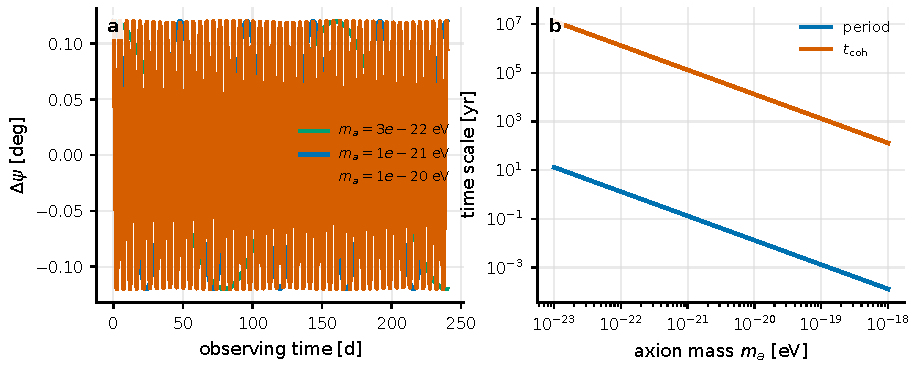
\includegraphics[width=0.94\linewidth]{figures/generated/chapter_15/ch15_axion_polarization_oscillation.pdf}
\caption{超轻暗物质把偏振旋转变成时间序列。左图画出三个轴子质量对应的 \(\Delta\psi(t)\)：质量越大、振荡越快。右图把质量 \(m_a\) 换算成周期 \(T_a\) 和相干时间 \(t_{\rm coh}\sim T_a/v^2\)（取 \(v=10^{-3}c\)）：越轻的轴子摆得越慢，却能在越长的时间里保持同一相位。}
\label{fig:e22-oscillation}
\end{figure}


\section{怎样测这么小的旋转：偏振分辨的强度与相干测量}
\label{sec:e22-measure}

目标信号常常小到 \(10^{-3}\) 弧度甚至更小。这一节要说清楚：我们凭什么、用什么数据结构去抓它，以及为什么"抓到一个非零角"往往首先是一个\emph{系统误差}问题，而不是发现。

\paragraph{偏振测量的本质：在偏振基上数光子}

回到第 \ref{chap:e18} 章打下的地基：偏振测量的本质，就是把一束光分到两个（或几个）正交偏振通道里，\emph{分别数光子}。用斯托克斯参量（Stokes parameters）\(I,Q,U,V\) 记账，线偏振信息全在 \(Q\)、\(U\) 里。一次偏振旋转 \(\beta\) 对 \(Q,U\) 的作用极其干净：把复组合 \(Q\pm iU\) 乘上一个相位因子，

\begin{equation}
  Q\pm iU \;\longrightarrow\; e^{\pm 2i\beta}\,(Q\pm iU).
  \label{eq:e22-qu-rotation}
\end{equation}
\begin{formulaexplain}
\(Q,U\)：线偏振斯托克斯参量；\(\beta\)：整体偏振旋转角。指数里那个 \(2\beta\)（不是 \(\beta\)）来自线偏振的"自旋 2"性质——偏振是一条无向的双箭头，转 \(180^\circ\) 就复原，所以数学上以 \(2\beta\) 出现。
\end{formulaexplain}

那个 \(2\) 很关键：它意味着一个很小的角度误差就足以让本该干净的模式互相污染。在球谐（\(E/B\) 模）空间里，\eqref{eq:e22-qu-rotation} 会把 \(E\) 模漏进 \(B\) 模。若源本身的奇宇称谱可忽略，旋转后出现的奇宇称谱近似为

\begin{equation}
  C_\ell^{EB,\rm obs}=\tfrac12\sin(4\beta)\,(C_\ell^{EE}-C_\ell^{BB}),
  \qquad
  C_\ell^{TB,\rm obs}=\sin(2\beta)\,C_\ell^{TE}.
  \label{eq:e22-eb-tb}
\end{equation}
\begin{formulaexplain}
\(C_\ell^{EB},C_\ell^{TB}\)：旋转后冒出来的奇宇称功率谱；\(\beta\)：旋转角。若源本征的 \(EB/TB\) 很小，非零的 \(EB/TB\) 就成了旋转角的探针——但探测器角度标定的错误会产生几乎一模一样的形状。
\end{formulaexplain}

\paragraph{宇宙双折射：为什么它首先是角标定问题}

宇宙微波背景（CMB）是找"全局偏振旋转"的诱人靶子：最后散射面极远，天区极大，统计量能压到很小。可它也把一个简单问题逼成最尖锐的系统误差问题。宇宙本身把偏振转了 \(\beta\)（宇宙双折射，cosmic birefringence），和探测器整体角度标定错了 \(\alpha\)，在 CMB 谱里长得几乎一样——两者都通过 \eqref{eq:e22-eb-tb} 冒出同样形状的 \(EB\)。代个数感受强度：\(\beta=0.35^\circ\) 时 \(\tfrac12\sin(4\beta)\simeq0.012\)，也就是 \(EB\) 泄漏只有 \(EE\!-\!BB\) 的百分之一量级——信号本就微弱，还和标定误差纠缠在一起。Planck 2018 的重新分析靠一个巧办法把两者部分撬开：CMB 旋转 \(\beta\) 只作用于最后散射面来的光，而银河前景偏振近在眼前、\emph{不}被宇宙旋转拧过，两者对频率和多极矩的依赖不同，于是可以同时拟合 \(\beta\) 和标定角 \(\alpha\)，给出 \(\beta=0.35\pm0.14^\circ\)（\(68\%\) 置信）。后续 WMAP+Planck、Planck PR4 的分析反复强调，尘埃自身的 \(EB\)、带通失配、\(I\to P\) 泄漏、交叉偏振响应和天区掩模的选择，仍是压在这个结果上的主要系统误差 \citep{2020PhRvL.125v1301M,2022NatRP...4..452K,2022PhRvD.106f3503E,2022PhRvL.128i1302D}。宇宙双折射的原始理论根据，可追到 Carroll、Field、Jackiw 等对赝标量场诱导旋光的讨论 \citep{1990PhRvD..41.1231C,1999PhRvL..83.1506L}。

\begin{figure}[tbp]
\centering
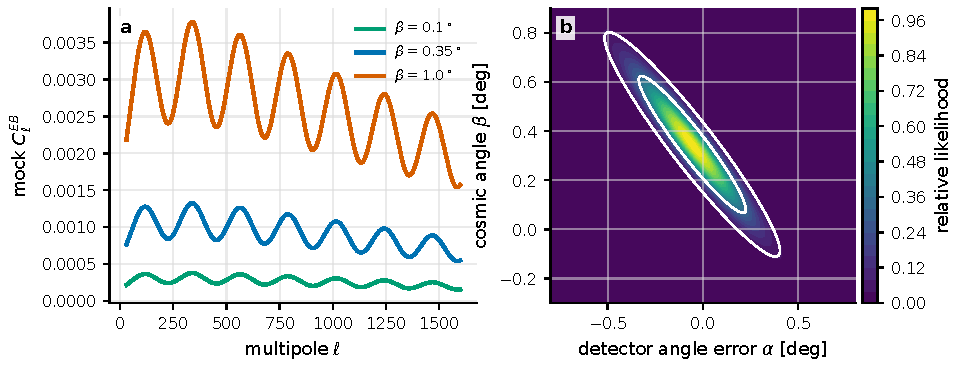
\includegraphics[width=0.94\linewidth]{figures/generated/chapter_15/ch15_cosmic_birefringence.pdf}
\caption{宇宙双折射同时牵动 \(E/B\) 混合与仪器角标定。左图用玩具 \(EE\)、\(BB\) 谱演示旋转角 \(\beta\) 怎样凭空生出 \(EB\)。右图画出标定角 \(\alpha\) 与宇宙旋转 \(\beta\) 的退化：只看 CMB，两者几乎等价；靠前景的频率依赖，才能把退化部分打破。}
\label{fig:e22-birefringence}
\end{figure}

\paragraph{把测量保留成事件表：不要过早平均}

\Needspace{10\baselineskip}
更一般地，最稳妥的做法是别急着把数据平均成"一张固定偏振角的图"，而是保留成一份\emph{偏振事件表}（沿用第 \ref{chap:e13} 章的事件表范式）。每个光子事件带上时间、频率、方向、偏振通道和权重：

\begin{equation}
  e_q=(t_q,\ \nu_q,\ \hat{\bm n}_q,\ p_q,\ w_q).
  \label{eq:e22-event}
\end{equation}
\begin{formulaexplain}
\(e_q\)：第 \(q\) 个偏振事件；\(t_q,\nu_q,\hat{\bm n}_q\)：到达时间、频率、天球方向；\(p_q\)：落进哪个偏振通道；\(w_q\)：质量权重。保留成事件表，就能在时间和频率维度上同时找"共同旋转"，而不必先把相位信息平均掉。
\end{formulaexplain}

若偏振角里藏着一个小的公共振荡 \(\delta\psi\)，落进某个偏振通道的概率就写成

\begin{equation}
  P\!\left(p_q\,\middle|\,t_q,\nu_q,\hat{\bm n}_q\right)
  = P_0\!\left[\,p_q\,\middle|\,\psi_{\rm src}
     +\psi_{\rm prop}(\nu_q,\hat{\bm n}_q)+\delta\psi(t_q,\hat{\bm n}_q)\,\right].
  \label{eq:e22-likelihood}
\end{equation}
\begin{formulaexplain}
\(\psi_{\rm src}\)：源本征偏振角；\(\psi_{\rm prop}\)：传播与仪器项（含法拉第、尘埃、仪器 Mueller 矩阵）；\(\delta\psi\)：要检验的新物理旋转。这条似然把"异常角度"拆成几类\emph{可以互相反驳}的来源，一起放进同一个拟合。
\end{formulaexplain}

代价也直白得吓人：如果仪器的 Mueller 矩阵非对角项只标定到 \(10^{-3}\)，而你要找的旋转也是 \(10^{-3}\) 弧度，那么系统误差已经和信号\emph{同量级}——这时候一个漂亮的非零角，多半是仪器在说话，不是宇宙。孤立中子星的光学偏振、磁星的 X 射线偏振、以及强场 QED 真空双折射的候选信号，都必须先把源的几何和传播效应建模干净，偏振异常才可能被解释成新物理 \citep{2017MNRAS.465..492M}。


\section{强场环境：致密天体作为轴子实验室}
\label{sec:e22-strongfield}

旋转通道靠的是轴子场本身；\emph{转换}通道则要借一片强磁场，把轴子和光子直接互相变身。哪里有最强的磁场？正是第 \ref{chap:e18} 章的致密天体（中子星、磁星）与第 \ref{chap:e19} 章的黑洞。这一节把偏振量子通道搬进中子星、磁星和黑洞的强场环境，既算转换概率，也接上超辐射的玻色云。

\paragraph{磁场里的轴子--光子转换}

在横向磁场 \(B_\perp\) 中，轴子只和与 \(B_\perp\) 平行的那个光子偏振态混合。弱混合、均匀磁场、吸收可忽略时，转换概率是

\begin{equation}
  P_{a\to\gamma}\simeq\left(\frac{g_{a\gamma}B_\perp L}{2}\right)^2
  \mathrm{sinc}^2\!\left(\frac{qL}{2}\right),
  \qquad
  q\simeq\frac{|m_a^2-m_\gamma^2|}{2E}.
  \label{eq:e22-conversion}
\end{equation}
\begin{formulaexplain}
\(P_{a\to\gamma}\)：轴子变光子的概率；\(B_\perp\)：横向磁场；\(L\)：相干路径长；\(E\)：能量；\(m_\gamma\)：等离子体里光子的有效质量；\(q\)：轴子与光子的动量失配。前面的平方给强度，\(\mathrm{sinc}^2\) 因子管相干：相位一失配，累积就被砍断。
\end{formulaexplain}

请把它和旋转公式 \eqref{eq:e22-rotation} 并排看，两种"距离依赖"的对比一目了然。当 \(qL\ll1\)（相干），\(\mathrm{sinc}^2\to1\)，概率按 \(L^2\) 增长——\textbf{转换是沿程累积的，走得越长越强}，这正好和"旋转只认两端点"相反。可一旦 \(qL\gtrsim\pi\)，不同路径段的转换振幅开始反相抵消，\(\mathrm{sinc}^2\) 迅速衰减，再长也没用。这就是相干长度的物理。地面实验把这个公式用到极致：CAST 用一块退役的 LHC 偶极磁体（\(9\,\mathrm T\)、\(9.26\,\mathrm m\)）盯着太阳，找太阳轴子转换成的 X 射线，其 2013--2015 真空管数据给出 \(g_{a\gamma}<0.66\times10^{-10}\,\mathrm{GeV^{-1}}\)（\(95\%\) 置信），适用于 \(m_a\lesssim0.02\,\mathrm{eV}\) 的相干低质量区 \citep{2017NatPh..13..584C}。

\begin{figure}[tbp]
\centering
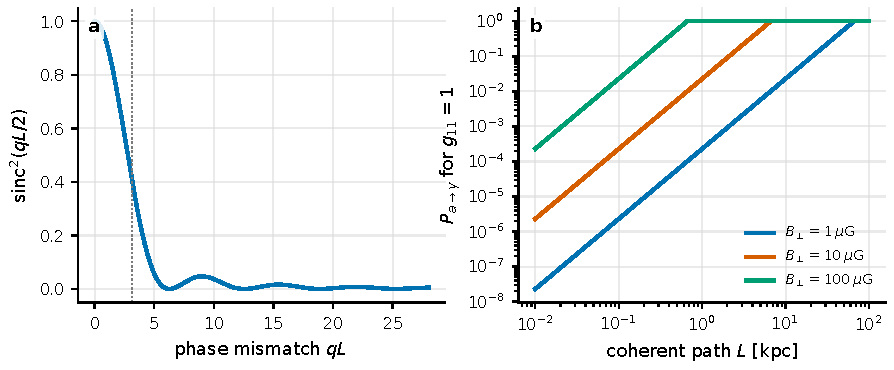
\includegraphics[width=0.94\linewidth]{figures/generated/chapter_15/ch15_axion_conversion.pdf}
\caption{轴子--光子转换由强度和相位共同决定。左图是相干因子 \(\mathrm{sinc}^2(qL/2)\)：当 \(qL\) 逼近 \(\pi\)，路径不同部分的转换振幅开始抵消。右图给出星际尺度的相干极限量级（取 \(g_{a\gamma}=10^{-11}\,\mathrm{GeV^{-1}}\)）：在 \(\mu\mathrm G\) 磁场、kpc 路径下，单段转换概率通常远小于 1。}
\label{fig:e22-conversion}
\end{figure}

\paragraph{磁星与 FRB：极端磁化的偏振实验室}

中子星和磁星把这一切推到极限——第 \ref{chap:e18} 章我们已经看到，磁星表面的磁场逼近临界场，连真空都成了双折射介质。这种环境对轴子转换是天然的放大器，但也意味着本征的偏振结构和传播前景都极强。快速射电暴（FRB）给了另一类极端样本：FRB~121102 落在 \(z=0.193\) 的宿主星系里，\(4\text{--}8\,\mathrm{GHz}\) 的暴发显示近乎 \(100\%\) 的线偏振，却带着高得离谱、还随时间变的法拉第旋转量 \(\mathrm{RM}_{\rm src}=1.46\times10^5\) 与 \(1.33\times10^5\,\mathrm{rad\,m^{-2}}\)，个别子结构窄到 \(\lesssim30\,\mu\mathrm s\)。若宿主贡献 \(\mathrm{DM_{host}}\sim70\text{--}270\,\mathrm{pc\,cm^{-3}}\)，反推出的视线磁场下限已达毫高斯（mG）量级，是普通银河系星际介质 \(\sim5\,\mu\mathrm G\) 的几百倍 \citep{2018Natur.553..182M}。这类源既是极端磁化等离子体的实验室，也是最狡猾的骗子：一个看似"无色"的偏振变化，仍要先排除有限通道宽度造成的退偏振、\(\mathrm{RM}\) 随时间漂移、以及等离子体透镜的选择效应，才轮到轴子。

\begin{figure}[tbp]
\centering
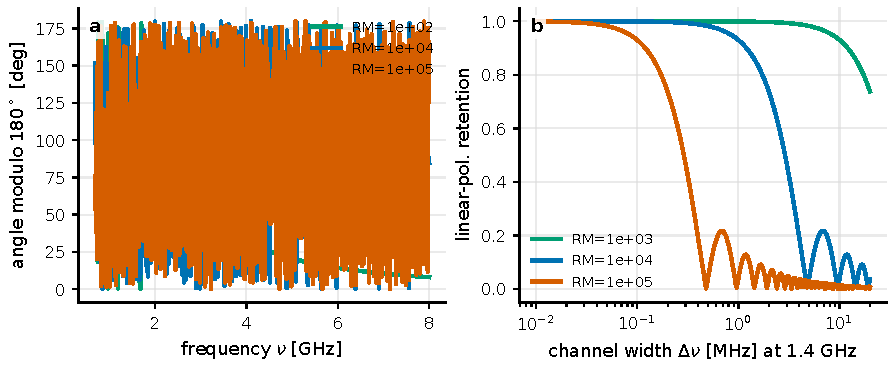
\includegraphics[width=0.94\linewidth]{figures/generated/chapter_15/ch15_frb_faraday_foreground.pdf}
\caption{FRB 的偏振前景能轻松淹没微弱旋转。左图画出不同 \(\mathrm{RM}\) 下偏振角随频率的 \(180^\circ\) 缠绕：\(\mathrm{RM}=10^5\,\mathrm{rad\,m^{-2}}\) 在 GHz 频段变化极快。右图是 \(1.4\,\mathrm{GHz}\) 附近有限通道宽度造成的线偏振保留率——要测这么高的 \(\mathrm{RM}\)，必须用极窄的通道。}
\label{fig:e22-frb}
\end{figure}

\paragraph{黑洞超辐射：把轻玻色场种在自转黑洞旁}

黑洞把轻玻色场和偏振图像连成一体。绕着自转（Kerr）黑洞的玻色波，只要频率足够低，满足

\begin{equation}
  \omega<m\,\Omega_H,
  \label{eq:e22-superradiance}
\end{equation}
\begin{formulaexplain}
\(\omega\)：玻色模频率；\(m\)：方位量子数（整数）；\(\Omega_H\)：Kerr 黑洞视界的角速度。满足这条不等式时，波会从黑洞自转里\emph{抽}走能量，指数增长，堆成一团绕黑洞旋转的玻色云。
\end{formulaexplain}

就能从黑洞自转里抽能量，指数放大，长成一团"超辐射玻色云"（superradiant boson cloud）。云能不能有效长起来，取决于轴子康普顿波长与黑洞尺度是否匹配。定义一个无量纲的"引力精细结构常数"

\begin{equation}
  \alpha_G=\frac{G M_\bullet m_a}{\hbar c},
  \label{eq:e22-alphaG}
\end{equation}
\begin{formulaexplain}
\(\alpha_G\)：黑洞引力半径与轴子康普顿波长之比；\(M_\bullet\)：黑洞质量。当 \(\alpha_G\sim0.1\text{--}1\) 时，玻色波"装得进"黑洞附近，超辐射增长最快。
\end{formulaexplain}

当 \(\alpha_G\sim0.1\text{--}1\)，玻色康普顿波长与黑洞尺度对上，云长得最凶。把 \eqref{eq:e22-alphaG} 反解，就把黑洞质量映射到它最敏感的轴子质量：

\begin{equation}
  m_a\simeq 1.34\times10^{-10}\,\mathrm{eV}\;\alpha_G
  \left(\frac{M_\odot}{M_\bullet}\right).
  \label{eq:e22-bh-mass}
\end{equation}
\begin{formulaexplain}
把黑洞质量 \(M_\bullet\) 换算成最敏感的轴子质量 \(m_a\)：黑洞越重，对应的轴子质量窗口越低。所以不同质量的黑洞，探的是超轻质量谱的不同段。
\end{formulaexplain}

代两个真实黑洞。银心 Sgr~A\(^*\)（\(4.3\times10^6\,M_\odot\)）在 \(\alpha_G=0.4\) 时对应 \(m_a\simeq1.2\times10^{-17}\,\mathrm{eV}\)；M87\(^*\)（\(6.5\times10^9\,M_\odot\)）则对应 \(8\times10^{-21}\,\mathrm{eV}\)——两个黑洞探的是完全不同的质量段。这里偏振通道又回来了：EHT 的偏振成像里，轴子云会让环上的偏振角随轴子周期一起摆动，Sgr~A\(^*\) 的周期约 \(100\text{--}1000\,\mathrm s\)，M87\(^*\) 可长到数天。能不能看见这种摆动，取决于空间分辨率——若分辨不开环上不同方位，摆动就会被"平均"抹平 \citep{2015LNP...906.....B,2015CQGra..32m4001B,2017PhRvD..96c5019B,2020PhRvL.124f1102C,2022NatAs...6..592C}。

\begin{figure}[tbp]
\centering
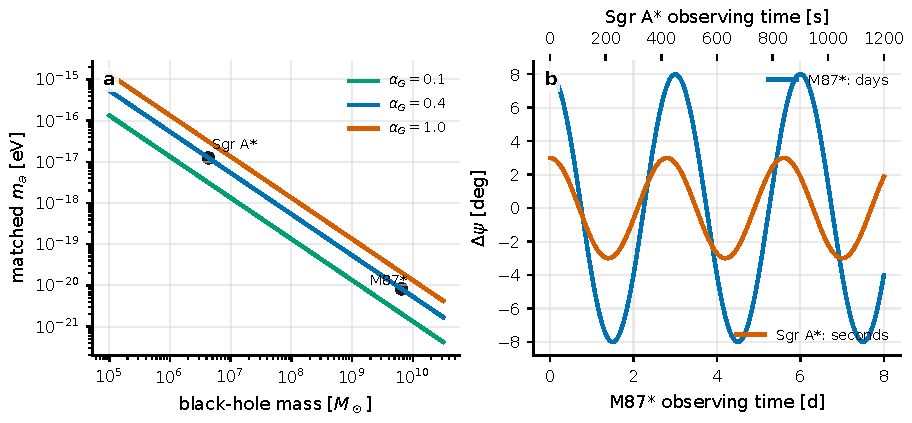
\includegraphics[width=0.94\linewidth]{figures/generated/chapter_15/ch15_black_hole_axion_cloud.pdf}
\caption{黑洞质量框定超辐射轴子的质量窗口。左图用 \(\alpha_G=GM_\bullet m_a/\hbar c\) 标出不同黑洞质量对应的 \(m_a\)：Sgr~A\(^*\) 与 M87\(^*\) 落在不同的超轻质量段。右图给出 EHT 偏振角振荡的两个典型时标：M87\(^*\) 可在天尺度采样，Sgr~A\(^*\) 则需要秒到分钟级的偏振成像。}
\label{fig:e22-bh}
\end{figure}


\section{把异常写成可反驳的检验}
\label{sec:e22-falsifiable}

走到这里，所有候选信号都共享一条铁律：\textbf{异常本身不是结论，异常的"可反驳结构"才是结论}。这一节把前面散落的招数收成一套统一的账本。

\paragraph{一份账本：把四类来源摊开对齐}

新物理搜索的观测量往往不止一个：偏振角、到达时间、像位置、放大率，可能来自不同仪器，各带各的统计与系统误差。把它们并成一个数据向量 \(\bm d\)，模型就拆成四大块：

\begin{equation}
  \bm m(\bm\theta)=\bm m_{\rm src}+\bm m_{\rm prop}+\bm m_{\rm inst}+\bm m_{\rm new}(\bm\theta),
  \label{eq:e22-model-vector}
\end{equation}
\begin{formulaexplain}
\(\bm m\)：模型预测向量；四项分别是源、传播、仪器、新物理。\(\bm\theta\)：新物理参数（\(g_{a\gamma}\)、\(m_a\)、\(\beta\)、子晕质量函数等）。这种拆分逼着我们把异常和普通天体物理、传播前景、校准误差摆进\emph{同一本账}里比较。
\end{formulaexplain}

在高斯近似下，拟合的目标函数是

\begin{equation}
  -2\ln\mathcal L=\big[\bm d-\bm m(\bm\theta)\big]^{\mathsf T}
  \big(C_{\rm stat}+C_{\rm sys}\big)^{-1}
  \big[\bm d-\bm m(\bm\theta)\big]
  +\ln\det\big(C_{\rm stat}+C_{\rm sys}\big).
  \label{eq:e22-likelihood-gauss}
\end{equation}
\begin{formulaexplain}
\(\mathcal L\)：高斯似然；\(C_{\rm stat}\)：统计协方差（光子噪声、到达时间误差、图像噪声）；\(C_{\rm sys}\)：系统误差协方差（Mueller 矩阵、绝对偏振角、法拉第前景、尘埃 \(EB\)、透镜宏模型……）。残差必须用两类误差\emph{一起}加权；漏掉 \(C_{\rm sys}\)，一个孤立异常就会被错误放大。
\end{formulaexplain}

这条式子把本章反复念叨的那句话数学化了：只要 \(C_{\rm sys}\) 没进似然，任何单个异常点都会被过度解释。

\paragraph{五把撬棍：让不同信号互相出卖}

好在这些信号有清清楚楚的相互区分方式，每一把都对应前面讲过的物理：

\begin{itemize}
\item \textbf{波长依赖。} 法拉第旋转随 \(\lambda^2\)（第 \ref{chap:e21} 章），轴子旋转近似无色（\eqref{eq:e22-rotation}）——测几个频率就能撬开。
\item \textbf{时间行为。} 静态宇宙双折射给一个不变的全局角（\eqref{eq:e22-eb-tb}），超轻暗物质给一条会呼吸的正弦（\eqref{eq:e22-osc-signal}）——测几十天到几年就能撬开。
\item \textbf{黑洞标度。} 超辐射云的偏振振荡应随黑洞质量、自转、环上方位和观测时间联动（\eqref{eq:e22-bh-mass}），普通吸积流不会这么"听黑洞的话"。
\item \textbf{路径依赖。} 转换按 \(L^2\) 沿程累积（\eqref{eq:e22-conversion}），旋转只认两端点——两者的距离响应正好相反。
\item \textbf{交叉检验。} 样本统计、空场或控制源、频率反演、时间相干性、仪器重标定，任何一项翻车，"发现"就该降级。
\end{itemize}

\paragraph{一个平行的通道：暗物质如何把质量变成角偏移}

偏振通道找的是"场对光子的量子影响"；还有一条平行的通道，找的是"暗物质质量分布对光线路径的影响"——引力透镜。它同样"无色"，同样不表现为"看到一团暗物质"，而表现为像位置、放大率或到达时间偏离普通模型。暗物质的存在本身有星系团碰撞（如子弹星团中弱透镜质量峰与 X 射线气体的分离，说明主质量近似无碰撞）、弱透镜和动力学多重支撑 \citep{2006ApJ...648L.109C,1993ApJ...404..441K}；而冷暗物质模拟预言银河晕里布满远低于可见卫星星系的子晕，成了强透镜异常的重要候选解释 \citep{1994ApJ...427L...1F,1999ApJ...524L..19M,2008Natur.454..735D}。子晕透镜的量级由爱因斯坦角给出，

\begin{equation}
  \theta_E=\left(\frac{4GM}{c^2}\frac{D_{ls}}{D_lD_s}\right)^{1/2},
  \qquad
  \delta\theta\simeq\frac{\theta_E^2}{b},
  \label{eq:e22-lensing}
\end{equation}
\begin{formulaexplain}
\(\theta_E\)：子晕爱因斯坦角，\(\propto M^{1/2}\)；\(M\)：透镜质量；\(D\)：观测者--透镜--源的距离组合；\(\delta\theta\)：像的天体测量偏移；\(b\)：像到子晕的角距离（\(b\gg\theta_E\)）。质量越大、越靠近像，位置扰动越明显；远离时按 \(1/b\) 衰减。
\end{formulaexplain}

数字把分辨率要求摆得很硬：在 \(D_l\simeq1\,\mathrm{Gpc}\)、\(D_s\simeq2\,\mathrm{Gpc}\) 的星系强透镜里，\(10^8\,M_\odot\) 子晕的 \(\theta_E\) 是几十毫角秒（mas），\(10^6\,M_\odot\) 只有几 mas；而 \(10^6\,M_\odot\) 子晕在 \(b=10\,\mathrm{mas}\) 处给出的天体测量偏移仅 \(\mu\mathrm{as}\) 量级。强透镜的流量比异常对放大率扰动敏感——Mao 与 Schneider 指出低质量子结构能解释一些四像系统的异常，Dalal 与 Kochanek 用 7 个射电透镜测得子结构质量分数中位数 \(f_{\rm sat}\simeq0.02\)（\(90\%\) 范围约 \(0.006\text{--}0.07\)），Vegetti、Hezaveh 等更用引力成像和 ALMA 把单个暗子结构的探测推进到空间分辨建模 \citep{1998MNRAS.295..587M,2002ApJ...572...25D,2010MNRAS.408.1969V,2016ApJ...823...37H}；Gaia 及未来天体测量巡天则把子晕横穿背景源变成时间域信号，主要限制来自扫描定律、源密度与自行协方差 \citep{2024MNRAS.531..632M,2016PhRvD..94h3504C}。这条通道与偏振通道的账本完全一致（\eqref{eq:e22-model-vector}）：暗子晕应\emph{同时}扰动像位置、放大率和时间延迟，而恒星表面结构主要随源自转、波长和基线方向变化——把这些区别放进同一个似然，异常才可能升格为发现。

\begin{figure}[tbp]
\centering
\includegraphics[width=0.94\linewidth]{figures/generated/chapter_15/ch15_dark_matter_lensing.pdf}
\caption{暗物质子晕的透镜信号受角尺度限制。左图给出典型 Gpc 几何下子晕爱因斯坦角随质量的变化。右图把 \(\delta\theta\simeq\theta_E^2/b\) 换成天体测量偏移：低质量子晕需要 mas 级的接近和 \(\mu\mathrm{as}\) 级的系统控制才可能看见。}
\label{fig:e22-lensing}
\end{figure}

\paragraph{一条时间域的旁证：脉冲星阵列}

同样的"共同时间项"逻辑，还能用在脉冲星身上。脉冲星有稳定相位、重复脉冲，天然适合做时间域阵列（脉冲星计时阵列，PTA）。超轻标量暗物质的引力势振荡会在计时残差里留下窄带信号：写成 \(\Psi_c\cos(2m_at+\varphi)\)，简化残差是

\begin{equation}
  R_\alpha(t)\simeq\frac{\Psi_c}{2\pi f}
  \Big[\sin(2\pi ft+\varphi_E)-\sin\!\big(2\pi f(t-D_\alpha/c)+\varphi_\alpha\big)\Big],
  \label{eq:e22-pta}
\end{equation}
\begin{formulaexplain}
\(R_\alpha\)：第 \(\alpha\) 颗脉冲星的计时残差；\(\Psi_c\)：势振荡幅度；\(f\simeq m_a/\pi\)：窄带频率；\(D_\alpha\)：脉冲星距离。第一项是所有脉冲星共享的"地球项"，第二项是每颗星各自的"脉冲星项"。
\end{formulaexplain}

\(m_a\sim10^{-23}\,\mathrm{eV}\) 对应 \(f\sim10^{-8}\,\mathrm{Hz}\)，正落在 PTA 的 \(10^{-9}\text{--}10^{-7}\,\mathrm{Hz}\) 窗口里。Porayko 与 Postnov 分析 NANOGrav 旧数据，给出 \(\Psi_c<1.14\times10^{-15}\)（\(95\%\) 置信）的上限 \citep{2014PhRvD..90f2008P}。这个标量模板的脉冲星间相关几乎不依赖两星夹角，因此不同于随机引力波背景那条著名的 Hellings--Downs 角相关曲线——这本身又是一把撬棍。若将来做"脉冲星偏振阵列"，同样要把共同地球项、本征磁层偏振、星际法拉第旋转、脉冲轮廓变化和接收机偏振泄漏一一分开。

\begin{figure}[tbp]
\centering
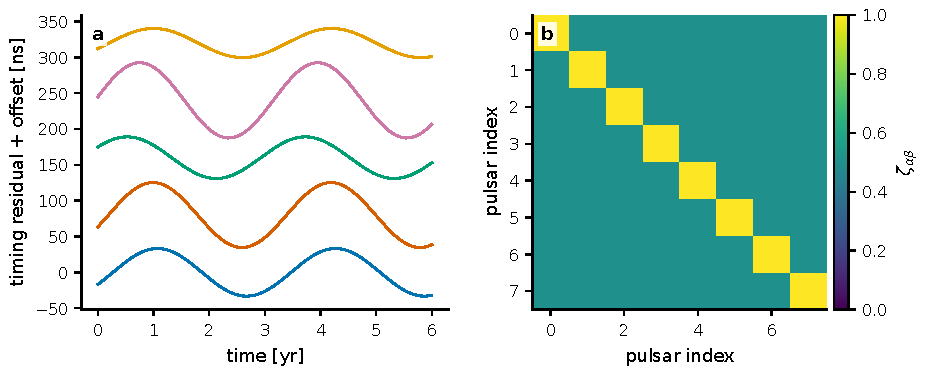
\includegraphics[width=0.94\linewidth]{figures/generated/chapter_15/ch15_pulsar_array_correlation.pdf}
\caption{脉冲星阵列里的共同窄带信号。左图是一个公共地球项叠加每颗星自己的脉冲星项（曲线人为错开以便观看）。右图给出标量势振荡模型的简化相关矩阵 \(\zeta_{\alpha\beta}=(1+\delta_{\alpha\beta})/2\)，它不同于随机张量引力波背景的角相关。}
\label{fig:e22-pta}
\end{figure}


\section{本章要点}
\label{sec:e22-summary}

\begin{itemize}
\item \textbf{一个耦合，两个观测量。} 极简的 \(a\,\bm E\cdot\bm B\) 耦合（\eqref{eq:e22-lagrangian}）同时打开两条量子通道：轴子背景\emph{拧转}线偏振面，强磁场里轴子和光子\emph{互相转换}。测的都是偏振，物理却互补。
\item \textbf{旋转角只认两端点，无色。} 相位差是全微分沿路径的积分，只留端点差（\eqref{eq:e22-phase-diff}），旋转角是它的一半（\eqref{eq:e22-rotation}），且\emph{不含波长}——这是与法拉第旋转（\(\propto\lambda^2\)）分家的第一把撬棍。
\item \textbf{暗物质让偏振呼吸。} 若轴子是超轻暗物质，场随时间振荡（\eqref{eq:e22-dm-field}），旋转角变成一条准单频正弦（\eqref{eq:e22-osc-signal}）；周期几十天、相干时间可达 \(10^5\) 年（\eqref{eq:e22-timescales}）——搜寻要在长时间基线上找共同摆动，而非只测一次。
\item \textbf{测量的本质是在偏振基上数光子。} 斯托克斯旋转的 \(2\beta\)（\eqref{eq:e22-qu-rotation}）会把 \(E\) 漏进 \(B\)（\eqref{eq:e22-eb-tb}）；CMB 双折射首先是 \(\beta\) 与标定角 \(\alpha\) 的退化问题，\(\beta=0.35\pm0.14^\circ\) 的结果全靠前景频率依赖撬开退化。把数据留成事件表（\eqref{eq:e22-event}、\eqref{eq:e22-likelihood}）才不至于过早平均掉信号。
\item \textbf{转换沿程累积，致密天体是放大器。} \(P_{a\to\gamma}\propto(g_{a\gamma}B_\perp L)^2\,\mathrm{sinc}^2(qL/2)\)（\eqref{eq:e22-conversion}）在相干区按 \(L^2\) 增长；磁星、FRB 的极端磁化和黑洞超辐射玻色云（\eqref{eq:e22-superradiance}--\eqref{eq:e22-bh-mass}）把偏振通道搬进强场，代价是本征结构与前景同样凶猛。
\item \textbf{异常要写成可反驳的账本。} 把源、传播、仪器、新物理拆开（\eqref{eq:e22-model-vector}），用 \(C_{\rm stat}+C_{\rm sys}\) 一起加权（\eqref{eq:e22-likelihood-gauss}）；靠波长、时间、黑洞标度、路径依赖和交叉检验这五把撬棍让信号互相出卖。透镜（\eqref{eq:e22-lensing}）与 PTA（\eqref{eq:e22-pta}）是同一逻辑的平行通道。
\end{itemize}

\noindent\textbf{想一想。}
（1）为什么轴子旋转公式 \eqref{eq:e22-rotation} 里"路径中间"的场值完全不出现，而转换公式 \eqref{eq:e22-conversion} 却对路径长 \(L\) 极其敏感？这两种"距离依赖"的差别，能怎样帮你在真实数据里把它们分开？
（2）如果一台望远镜的偏振角标定误差是 \(0.5^\circ\)，你要找的宇宙双折射是 \(0.35^\circ\)，你有没有办法\emph{只}靠这一台仪器把两者分开？为什么"利用前景的频率依赖"能救场？
（3）Sgr~A\(^*\) 与 M87\(^*\) 探的是完全不同的轴子质量段（\eqref{eq:e22-bh-mass}）。假如某天在 M87\(^*\) 的环上看到偏振角以数天周期振荡，你会先怀疑它是轴子云，还是先怀疑吸积流本身？要用哪些交叉检验才敢升格为"发现"？

\chapter{宇宙学中的量子问题}
\label{chap:e23}

\begin{chapteropening}
前几章我们把望远镜对准一颗恒星、一个吸积盘、一次爆发——那些源你可以换个夜晚再看一遍，可以调带宽、可以重做实验。这一章的对象只有一个，而且只有一次：\textbf{整个宇宙}。它是一场早已发生、无法重启的光学实验，我们只是很晚才架起探测器，去读它留在天空上的一张底片。这张底片就是宇宙微波背景（cosmic microwave background，CMB）——一片几乎完美的黑体微波天空，上面叠着 \(10^{-5}\) 量级的温度花纹和更弱的偏振结构。

本章要回答三个层层递进的问题。第一，\textbf{这些花纹是从哪来的}？我们会看到它们的种子是暴胀期间被放大的\emph{量子}真空涨落，以及一个关键转折：这些量子涨落如何通过退相干（decoherence）"变成"可以用经典随机场描述的密度扰动。第二，\textbf{一束光跨越几十亿光年会经历什么}？它的偏振可能被悄悄转过一个小角，它的到达时间可能被介质和更深的物理拉开。第三，\textbf{我们能不能用一根宇宙学长的基线去称量最基本的物理}——洛伦兹不变性、光子的质量上限？把抽象的宇宙学，一步步落回本书熟悉的相干、偏振与光子到达时间上。
\end{chapteropening}

\section{宇宙作为一次不可重做的光学实验}
\label{sec:e23-lightfield}

先建立画面。谈 CMB 时人们张口就是"暴胀量子涨落"，但观测的入口其实非常朴素：望远镜先看到一个几乎完美的黑体微波天空，然后在这个平均背景上，去测一层薄薄的角向涨落。所以本节先把 CMB 当成一个\emph{光场}来称量，再一路退回到产生这些花纹的早期量子模式。

平均的 CMB 是一个温度 \(T_0=2.7255\pm0.0006\,{\rm K}\) 的黑体。第 \ref{chap:e05} 章把光场量子化、写出普朗克黑体公式，第 \ref{chap:e06} 章又专门讲了热态（thermal state）：一个热光场里每个频率模式的平均光子占据数由玻色分布给出，比强度再由普朗克公式给出：
\begin{equation}
  n_\nu=\frac{1}{\exp(h\nu/k_{\rm B}T_0)-1},
  \qquad
  I_\nu=\frac{2h\nu^3}{c^2}\,n_\nu .
  \label{eq:e23-planck-spectrum}
\end{equation}
\begin{formulaexplain}
\(n_\nu\) 是单个频率模式里的平均光子数，\(I_\nu\) 是黑体比强度。低频端 \(n_\nu\) 大，场接近经典热光；高频端 \(n_\nu<1\)，单模里常常连一个光子都不到。
\end{formulaexplain}
逐个符号落地：\(\nu\) 单位 Hz，\(h\) 是普朗克常数，\(k_{\rm B}\) 是玻尔兹曼常数，\(I_\nu\) 的单位是 \({\rm erg\,s^{-1}\,cm^{-2}\,Hz^{-1}\,sr^{-1}}\)（CMB 文献常换成 \({\rm MJy\,sr^{-1}}\)）。代两个真实频率进去感受一下：在 \(30\,{\rm GHz}\)，\(h\nu/k_{\rm B}T_0\simeq0.53\)，于是 \(n_\nu\simeq1/(e^{0.53}-1)\simeq1.4\)，低频通道仍是接近经典的热场；在 \(150\,{\rm GHz}\)，指数变大，\(n_\nu\simeq0.07\)，单模占据数已经小于 1。黑体强度峰落在 \(160\,{\rm GHz}\) 附近——这正是 Planck 高频仪器和许多地面实验把通道选在 \(90/150/220\,{\rm GHz}\) 的物理原因。FIRAS 把这个平均谱测得极其接近理想黑体，所以现代宇宙学干脆把平均谱当作\emph{已知背景}，把全部信息放进它上面的角向涨落和偏振里 \citep{1994ApJ...420..439M,1996ApJ...473..576F,2009ApJ...707..916F}。

把天空上的涨落展开成球谐（spherical harmonics），就像把一段声音展开成不同音高：
\begin{equation}
  T(\hat{\bm n})=T_0\,[1+\Theta(\hat{\bm n})],
  \qquad
  \Theta(\hat{\bm n})=\sum_{\ell m}a^{T}_{\ell m}\,Y_{\ell m}(\hat{\bm n}).
  \label{eq:e23-temperature-expansion}
\end{equation}
\begin{formulaexplain}
\(\Theta\) 是无量纲温度涨落，\(a^{T}_{\ell m}\) 是球谐系数，\(Y_{\ell m}\) 是球谐函数。这条式子把一张天空图拆成一层层角尺度：\(\ell\) 定尺度，\(m\) 管同一尺度上的方位花样。
\end{formulaexplain}
这里 \(\hat{\bm n}\) 是天空方向（一个单位矢量），多极矩 \(\ell\) 与角尺度近似满足 \(\theta\simeq180^\circ/\ell\)：\(\ell\simeq2\) 是半个天空那么大的花纹，\(\ell\simeq200\) 约一度，\(\ell\simeq2000\) 只有几角分。COBE 的差分微波辐射计首次在全天图上看到 \(\Delta T/T\sim10^{-5}\) 的结构，Planck 则把它一直分解到 \(\ell\sim2500\)。对一个各向同性的高斯天空，把同一个 \(\ell\) 上的 \(m\) 全部平方平均，就得到角功率谱（angular power spectrum）：
\begin{equation}
  \widehat C^{TT}_\ell=\frac{1}{2\ell+1}\sum_{m=-\ell}^{\ell}\bigl|a^{T}_{\ell m}\bigr|^2,
  \qquad
  D^{TT}_\ell=\frac{\ell(\ell+1)}{2\pi}\,C^{TT}_\ell .
  \label{eq:e23-cl-estimator}
\end{equation}
\begin{formulaexplain}
\(\widehat C^{TT}_\ell\) 是温度角功率谱估计量，来自一个 \(\ell\) 上全部 \(2\ell+1\) 个 \(m\) 模式的平均；\(D_\ell\) 是画图常用的重标度形式。这个平均就是 CMB 二点统计的核心压缩。
\end{formulaexplain}
若 \(a_{\ell m}\) 以 \(\mu{\rm K}\) 为单位，则 \(C_\ell\) 和 \(D_\ell\) 的单位是 \(\mu{\rm K}^2\)。\(D^{TT}_\ell\) 的第一声学峰在 \(\ell\simeq220\) 处，峰高约 \(5\times10^3\,\mu{\rm K}^2\)。这些峰不是随机的，它们来自复合（recombination）前光子—重子流体的\emph{声学振荡}：重子密度改变压缩峰的高度，暗物质密度改变引力势的衰减，角直径距离把物理声学尺度投影成天上的角尺度。Planck 用一个六参数的平直 \(\Lambda{\rm CDM}\) 模型拟合这些峰，给出 \(\Omega_bh^2\simeq0.0224\)、\(\Omega_ch^2\simeq0.120\)、\(n_s\simeq0.965\)、\(H_0\simeq67.4\,{\rm km\,s^{-1}\,Mpc^{-1}}\) 这样的典型精度 \citep{1992ApJ...396L...1S,1996ApJ...469..437S,2020A&A...641A...5P,2020A&A...641A...6P}。这里 \(\Omega_x\) 是第 \(x\) 种成分的无量纲密度参数（该成分密度与临界密度之比），\(h\equiv H_0/(100\,{\rm km\,s^{-1}\,Mpc^{-1}})\) 是约化哈勃常数，之所以写成 \(\Omega h^2\) 的组合，是因为 CMB 直接约束的是物理密度而与 \(H_0\) 的取值无关——这些都是六参数拟合的输出，若想细究记号的来历，可查任一本宇宙学教材，本书只把它们当作已知数字使用。

这里有一个"只有一次"的宇宙学专属限制。即使仪器完美无噪声，每个 \(\ell\) 上天空也只给你 \(2\ell+1\) 个 \(m\) 模式——样本就这么多，方差躲不掉。这叫宇宙方差（cosmic variance）：
\begin{equation}
  \frac{\sigma(C_\ell)}{C_\ell}=\sqrt{\frac{2}{(2\ell+1)\,f_{\rm sky}}} .
  \label{eq:e23-cosmic-variance}
\end{equation}
\begin{formulaexplain}
\(\sigma(C_\ell)/C_\ell\) 是样本方差带来的相对误差，\(f_{\rm sky}\) 是有效天区比例。低 \(\ell\) 可用模式少，所以大角尺度天生就有一层无法靠灵敏度消除的统计不确定性。
\end{formulaexplain}
\(f_{\rm sky}\) 是被使用的天空比例（银河面和强前景要被遮掉，故通常 \(f_{\rm sky}<1\)）。代数字：全天 \(\ell=2\) 的相对误差约 \(\sqrt{2/5}\simeq63\%\)，\(\ell=200\) 降到约 \(7\%\)，\(\ell=2000\) 只剩约 \(2.2\%\)。这就是为什么"低 \(\ell\) 反常""四极矩偏低"这类现象要放进有限模式数的协方差里判断，而不能只凭它在图上看起来显眼。这与第 \ref{chap:e15} 章的误差预算是同一种精神：先问"我到底有多少独立信息"。

偏振图比温度图多两个 Stokes 参数 \(Q\) 和 \(U\)。它们不是标量，而是随坐标旋转的\emph{自旋 2}（spin-2）量，所以要用自旋球谐函数展开，再线性组合成两种宇称明确的模式：
\begin{equation}
  (Q\pm iU)(\hat{\bm n})=\sum_{\ell m}a_{\pm2,\ell m}\,{}_{\pm2}Y_{\ell m}(\hat{\bm n}),
  \quad
  a^{E}_{\ell m}=-\tfrac12(a_{2,\ell m}+a_{-2,\ell m}),
  \quad
  a^{B}_{\ell m}=\tfrac{i}{2}(a_{2,\ell m}-a_{-2,\ell m}).
  \label{eq:e23-eb-definition}
\end{equation}
\begin{formulaexplain}
\(Q\pm iU\) 是自旋 \(\pm2\) 的偏振场，\({}_{\pm2}Y_{\ell m}\) 是自旋球谐函数，\(a^{E/B}_{\ell m}\) 是 E/B 模系数。这个组合把逐点的偏振方向翻译成全天上的两类图样。
\end{formulaexplain}
关键的物理在于宇称：\(E\) 模在镜像变换下像标量（偏振方向沿冷热斑呈放射或同心花样），\(B\) 模像赝标量（带旋涡感）。线性阶的标量密度涨落主要产生 \(T\) 和 \(E\)，\emph{不}直接产生原初 \(B\)。能产生 \(B\) 的只有几类：原初张量扰动（引力波）、弱引力透镜、偏振角被整体旋转、以及银河尘埃和同步辐射前景。记住这一点：\textbf{\(B\) 模是稀客}，谁能干净地造出它，谁就携带了最深的宇宙学信息。这条线索会在本章后面两次被拉动——一次指向原初引力波，一次指向偏振双折射。这两幅光场骨架图，见图~\ref{fig:e23-blackbody} 与图~\ref{fig:e23-power}。

\begin{figure}[tbp]
\centering
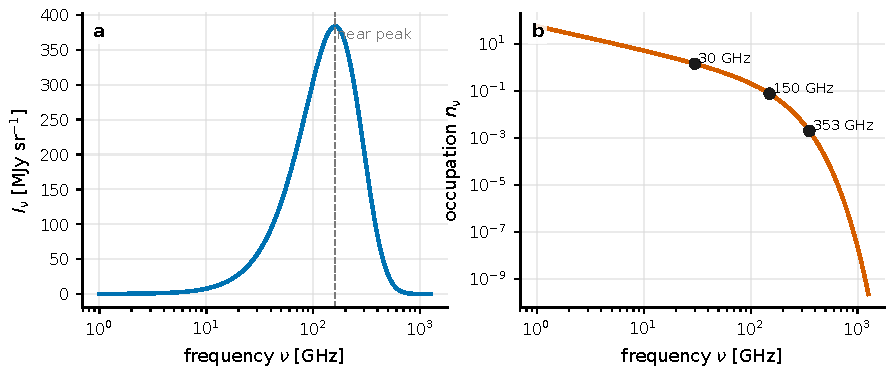
\includegraphics[width=0.9\linewidth]{figures/generated/chapter_16/ch16_cmb_blackbody.pdf}
\caption{CMB 的平均光场由黑体谱和模式占据数共同决定。左图把 \(T_0=2.7255\,{\rm K}\) 的普朗克谱写成 \({\rm MJy\,sr^{-1}}\)，峰值在 \(160\,{\rm GHz}\) 附近；右图是同一黑体在不同频率的单模平均光子数 \(n_\nu\)，低频通道占据数较高，高频通道逐渐进入 \(n_\nu<1\)。}
\label{fig:e23-blackbody}
\end{figure}

\begin{figure}[tbp]
\centering
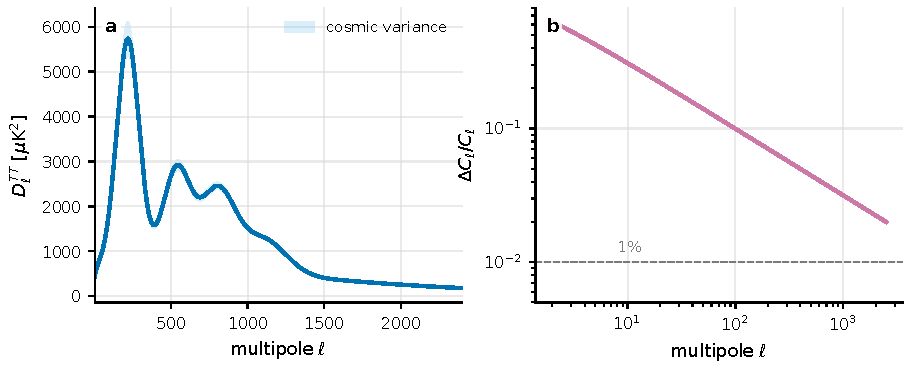
\includegraphics[width=0.9\linewidth]{figures/generated/chapter_16/ch16_cmb_power_spectrum.pdf}
\caption{角功率谱把天空涨落压缩到多极矩空间。左图是带声学峰和阻尼尾的 \(D_\ell^{TT}\)，阴影表示全天宇宙方差的量级；右图单独画出 \(\sqrt{2/(2\ell+1)}\)，说明大角尺度的误差由天上可用模式数决定，望远镜再灵敏也消不掉这部分方差。}
\label{fig:e23-power}
\end{figure}

\section{暴胀：把真空涨落放大成密度扰动}
\label{sec:e23-inflation}

上一节的 \(C_\ell\) 是天空上的统计量；暴胀（inflation）理论要解释的，是这些统计量为什么\emph{近似高斯}、\emph{近似尺度不变}、而且声学峰的相位是固定的（不是一团随机相位的杂波）。这里不能把 CMB 当成一束可反复制备的实验室光，而要把早期宇宙里每一个场模式，看成第 \ref{chap:e04} 章那个熟悉的量子谐振子——只不过它的频率随宇宙膨胀而变。

对标量曲率扰动 \(\mathcal R\)，人们定义一个把背景演化"打包"进去的 Mukhanov–Sasaki 变量 \(v\)：
\begin{equation}
  v(\bm x,\eta)=z(\eta)\,\mathcal R(\bm x,\eta),
  \qquad
  z=\frac{a\,\dot\phi}{H} .
  \label{eq:e23-ms-variable}
\end{equation}
\begin{formulaexplain}
\(v\) 是 Mukhanov–Sasaki 变量，\(\mathcal R\) 是我们最终关心的曲率扰动，\(z=a\dot\phi/H\) 把暴胀的背景演化装进一个系数里。用 \(v\) 写方程，每个傅里叶模就变成一个时变频率的量子谐振子。
\end{formulaexplain}
逐个符号：\(\eta\) 是共形时间（conformal time，满足 \({\rm d}\eta={\rm d}t/a\)），\(a\) 是尺度因子（无量纲，今天取 1），\(\phi\) 是驱动暴胀的背景标量场，\(H=\dot a/a\) 是哈勃率（单位 \({\rm s^{-1}}\)），点表示对宇宙时求导。把二阶作用量对每个傅里叶模 \(v_k\) 展开，就得到一条形式极其干净的运动方程：
\begin{equation}
  v_k''+\Bigl(k^2-\frac{z''}{z}\Bigr)v_k=0 .
  \label{eq:e23-ms-equation}
\end{equation}
\begin{formulaexplain}
\(v_k\) 是共动波数 \(k\) 的模式函数，撇号是对共形时间 \(\eta\) 的导数。方括号里 \(k^2-z''/z\) 就是这个"时变谐振子"的有效频率平方，符号的翻转正是暴胀的全部魔法所在。
\end{formulaexplain}
\(k\) 是共动波数（comoving wavenumber，单位 \({\rm Mpc^{-1}}\)）。这条方程的两种极限决定一切，逐一读出来：

\emph{亚视界}（\(k\gg aH\)）时，\(z''/z\) 相比 \(k^2\) 可忽略，方程退化成 \(v_k''+k^2v_k=0\)——一个普通简谐振子。取它的量子真空（Bunch–Davies 真空），归一化模式函数是
\[
  v_k(\eta)\simeq\frac{e^{-ik\eta}}{\sqrt{2k}} .
\]
这就是本书从头讲到尾的"最低能量态里仍在抖动"的真空涨落，只不过发生在早期宇宙的每一个短波模式上。

\emph{出视界}（\(k\simeq aH\)，之后 \(k\ll aH\)）时，膨胀把 \(z''/z\) 顶了上来并主导方程。此时增长解不再振荡而被\emph{冻结}，衰减解迅速缩小，于是 \(\mathcal R_k=v_k/z\) 趋于一个近似常数。"冻结"不是说模式停止演化，而是说相空间里一个方向被强烈压窄，最后只剩一个随机幅度，去支配后来的密度扰动 \citep{1988JETP...67.1297M,1990PhRvD..42.3413G,1996CQGra..13..377P}。

把这个冻结下来的二点统计，写成无量纲的原初曲率功率谱：
\begin{equation}
  \langle\mathcal R_{\bm k}\mathcal R_{\bm k'}\rangle
  =(2\pi)^3\delta^{(3)}(\bm k+\bm k')\,\frac{2\pi^2}{k^3}\,\mathcal P_{\mathcal R}(k),
  \qquad
  \mathcal P_{\mathcal R}(k)=A_s\Bigl(\frac{k}{k_*}\Bigr)^{n_s-1} .
  \label{eq:e23-primordial-spectrum}
\end{equation}
\begin{formulaexplain}
\(\mathcal P_{\mathcal R}\) 是无量纲原初曲率功率谱，\(A_s\) 是振幅，\(n_s\) 是谱指数（spectral index），\(k_*\) 是参考波数（pivot）。它把早期量子涨落的二点统计浓缩成今天 CMB 拟合里最核心的两个数。
\end{formulaexplain}
Planck 常取 pivot \(k_*=0.05\,{\rm Mpc^{-1}}\)，给出 \(\ln(10^{10}A_s)\simeq3.04\)，即 \(A_s\simeq2.1\times10^{-9}\)。谱指数 \(n_s=1\) 是精确的尺度不变；实测 \(n_s\simeq0.965\) 说明有一点"红倾"，长波略强于短波——这正是慢滚暴胀预期的微小偏离。请把这个数量级链条记牢：一个 \(10^{-9}\) 的原初曲率功率，经过辐射转移函数、声学振荡、复合面的有限厚度和后来的透镜平滑，被投影成今天天上 \(\Delta T/T\sim10^{-5}\) 的花纹 \citep{2020A&A...641A...6P,2020A&A...641A..10P}。

现在把它翻译成本书的量子光学语言。暴胀的时变背景，恰好把 \(\bm k\) 和 \(-\bm k\) 这一对模式，从真空演化成一个\emph{两模压缩态}（two-mode squeezed state）——第 \ref{chap:e06} 章介绍压缩态时说过，压缩就是"把一对模式的涨落成对放大，同时保持固定的相位关系"：
\begin{equation}
  |\psi\rangle=\prod_{\bm k}\exp\!\Bigl[\,r_k e^{-2i\varphi_k}\,\hat a_{\bm k}\hat a_{-\bm k}
  -r_k e^{2i\varphi_k}\,\hat a^\dagger_{\bm k}\hat a^\dagger_{-\bm k}\Bigr]\,|0\rangle .
  \label{eq:e23-squeezed-state}
\end{equation}
\begin{formulaexplain}
\(|\psi\rangle\) 是 \(\bm k\) 与 \(-\bm k\) 成对的两模压缩态，\(r_k\) 是压缩强度，\(\varphi_k\) 是压缩角，\(\hat a,\hat a^\dagger\) 是湮灭与产生算符。暴胀把真空涨落成对放大，并锁死它们的相位。
\end{formulaexplain}
每对模式的平均占据数是 \(N_k=\sinh^2 r_k\)。经过 \(50\text{--}60\) 个 e-folds（膨胀量级的对数）后 \(r_k\) 非常大，\(N_k\) 指数式增长。要提醒的是：这里的"占据数"指早期\emph{场模式}的量子激发数，和望远镜今天真正数到的 CMB 光子数不是一回事。在相空间里，压缩把 Wigner 函数拉成一条极细长的椭圆：一个方向被拉长（就是后来当作经典随机幅度的那个），另一个方向被压到很窄。正是这条被压死的方向，锁定了固定相位，从而在 \(TT\)、\(TE\)、\(EE\) 谱里排出一串规整的声学峰，而不是随机杂波（图~\ref{fig:e23-squeezed}）\citep{1990PhRvD..42.3413G,1996CQGra..13..377P,2006CQGra..23.2317P}。

\begin{figure}[tbp]
\centering
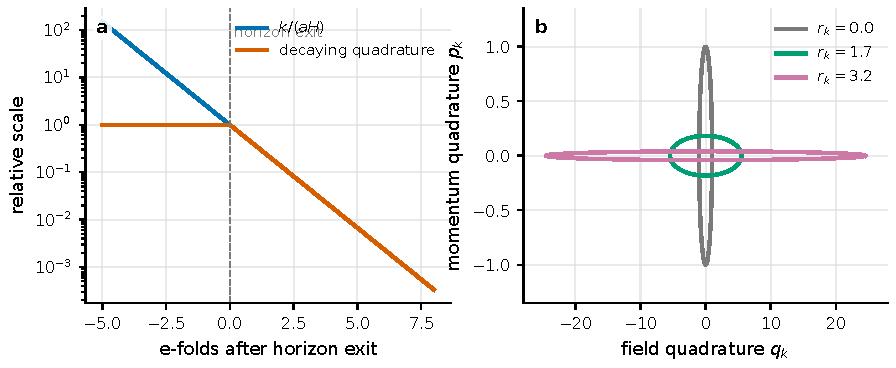
\includegraphics[width=0.9\linewidth]{figures/generated/chapter_16/ch16_squeezed_modes.pdf}
\caption{暴胀中的模式放大可以看成两模压缩。左图显示 \(k/(aH)\) 在穿出视界后指数下降，衰减方向被压窄；右图画相空间椭圆，\(r_k\) 增大时一个方向被拉长、另一个被压死，观测到的是后来表现为经典随机幅度的那条长轴。}
\label{fig:e23-squeezed}
\end{figure}

\section{退相干：量子涨落如何"变成"经典密度扰动}
\label{sec:e23-decoherence}

上一节留下一个不安：如果每个模式仍是一个纯的量子压缩态，它就是量子叠加，怎么能直接当成经典的密度涨落去算星系怎么长出来？答案是退相干（decoherence）。这也是本章第一个真正的"量子问题"：\textbf{一个被放大的量子态，为什么在观测上表现得像一个经典随机场}？

先给画面。一个量子态的"量子性"，藏在它密度矩阵的\emph{非对角项}里——那是不同幅度分支之间还能互相干涉的证据。可这些暴胀模式并不孤立：它们和一大堆没被观测的自由度纠缠在一起（未观测的短波模式、张量与标量的相互作用、复合前等离子体的自由度、透镜势，乃至数据分析里被边缘化掉的前景与仪器模式）。一旦把这些环境求和积掉，观测变量 \(q_k\) 的约化密度矩阵，非对角项就被一个高斯因子迅速压平：
\begin{equation}
  \rho_{\rm red}(q,q')=\rho_0(q,q')\,\exp\!\bigl[-\Gamma_k\,(q-q')^2\bigr] .
  \label{eq:e23-decoherence-density}
\end{equation}
\begin{formulaexplain}
\(\rho_{\rm red}\) 是观测变量 \(q_k\) 的约化密度矩阵，\(\rho_0\) 是未退相干的形式，\(\Gamma_k\) 衡量环境把非对角项压平的强度。当 \(q\ne q'\) 的相干项被压死，功率谱就可以用经典随机场去算。
\end{formulaexplain}
逐字读这条式子：\(q,q'\) 是同一个观测变量的两个不同取值，\((q-q')\) 越大代表两个分支相隔越远；指数因子 \(\exp[-\Gamma_k(q-q')^2]\) 是一口"钟形阀门"，把相隔较远的分支之间的干涉几乎完全关掉。\(\Gamma_k\) 的量纲取决于 \(q_k\) 怎样归一化，但物理判据很干脆：只要 \(\Gamma_k(\Delta q)^2\gg1\)，不同幅度分支之间就再也不会干涉，二点函数、角功率谱 \(C_\ell\)、角向三点谱（bispectrum）、透镜重建都可以按经典随机场老老实实地算。对暴胀模式，压缩越强、纠缠越深，\(\Gamma_k\) 越大，这个条件被极大幅度地满足——这正是"量子涨落变成经典密度扰动"这句话的精确含义。

要防止误解，说两句边界。退相干让\emph{统计}变经典，但它并没有替我们回答"到底是哪一个分支被实现了"——早期宇宙的"测量问题"在概念层面仍有争论。不过对我们能测的量（\(C_\ell\)、透镜重建、更高阶相关）来说，残留的相干相位信息太少，早已不足以撑起一次实验室式的 Bell 测试，也无法把 CMB 当成一个可反复制备的非经典态去操控 \citep{1996CQGra..13..377P,2006CQGra..23.2317P}。这与第 \ref{chap:e24} 章的量子网络望远镜恰成对照：那里你能主动制备、调制、重测量子态；这里，宇宙只给你一张不可重拍的底片，量子性早在复合之前就"沉淀"成了经典统计。

\section{涨落怎样产生：非高斯性与原初引力波}
\label{sec:e23-tensors}

二点函数（也就是 \(C_\ell\)）告诉我们\emph{有多少}涨落；要问这些涨落\emph{怎样产生}，得看两样更难测的东西：更高点函数（非高斯性）和张量模（原初引力波）。前者检验暴胀期间的相互作用与场内容，后者直指是否存在一份原初引力波背景。两者都极诱人，也都极易被有限模式数、透镜、尘埃和模板选择所限制。

若 \(\mathcal R\) 是严格高斯场，全部信息就都在二点函数里，三点及以上一律为零。可只要暴胀里有相互作用、非平凡声速、多场转移或尖锐特征，就会漏出非高斯性。它的主角是三点函数：
\begin{equation}
  \langle\mathcal R_{\bm k_1}\mathcal R_{\bm k_2}\mathcal R_{\bm k_3}\rangle
  =(2\pi)^3\delta^{(3)}(\bm k_1+\bm k_2+\bm k_3)\,B_{\mathcal R}(k_1,k_2,k_3) .
  \label{eq:e23-bispectrum}
\end{equation}
\begin{formulaexplain}
\(B_{\mathcal R}\) 是曲率扰动的三点谱（bispectrum），delta 函数强迫三个波矢首尾相接、闭合成一个三角形。三角形的\emph{形状}对应不同的早期宇宙相互作用，所以三点函数是非高斯性的主要语言。
\end{formulaexplain}
不同"形状"给出不同信号：local 型在\emph{扁长}三角形里最强（\(k_1\ll k_2\simeq k_3\)），equilateral 型在\emph{等边}三角形里最强，orthogonal 型是为区分不同相互作用而人为构造的近似正交模板。其中 local 型有一个很直观的实空间写法：
\begin{equation}
  \mathcal R(\bm x)=\mathcal R_g(\bm x)+\frac{3}{5}f^{\rm local}_{\rm NL}
  \Bigl[\mathcal R_g^2(\bm x)-\langle\mathcal R_g^2\rangle\Bigr] .
  \label{eq:e23-local-fnl}
\end{equation}
\begin{formulaexplain}
\(\mathcal R_g\) 是纯高斯场，\(f^{\rm local}_{\rm NL}\) 是 local 型非高斯的振幅。那个二次项让\emph{长波}去调制\emph{短波}的功率，所以 local 模板在扁长三角形里最敏感。
\end{formulaexplain}
\(f_{\rm NL}\) 无量纲。Planck 用温度加偏振给出 \(f^{\rm local}_{\rm NL}=-0.9\pm5.1\)、\(f^{\rm equil}_{\rm NL}=-26\pm47\)、\(f^{\rm orth}_{\rm NL}=-38\pm24\)（\(68\%\) 置信），都与零相容——没有发现标准模板下的显著非高斯性（图~\ref{fig:e23-nongaussian}）。这其实是对最简暴胀的一次有力支持：单场慢滚暴胀有一条"一致性关系"，预言扁长极限的 local 非高斯极小，数量级与 \(1-n_s\) 相当（也就是百分之几），\(f_{\rm NL}\) 天然就该很小 \citep{2003JHEP...05..013M,2020A&A...641A...9P,2020A&A...641A..10P}。

\begin{figure}[tbp]
\centering
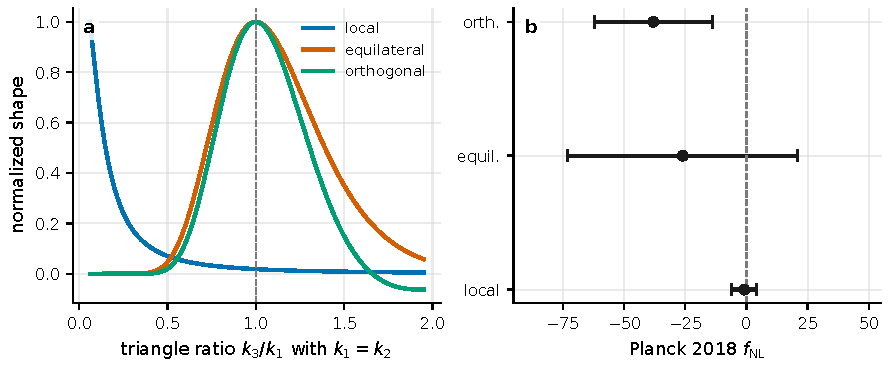
\includegraphics[width=0.9\linewidth]{figures/generated/chapter_16/ch16_non_gaussian_templates.pdf}
\caption{非高斯性由三角形构型和振幅共同决定。左图用 \(k_1=k_2\) 的切片比较 local、equilateral 与 orthogonal 三种模板的形状；local 型在扁长极限增强，equilateral 型在三边接近相等时最大。右图给出 Planck 对三个常用 \(f_{\rm NL}\) 的代表性约束，误差条都与零相容。}
\label{fig:e23-nongaussian}
\end{figure}

张量扰动是量子引力背景最直接的 CMB 目标——它就是暴胀产生的原初引力波，会在偏振里留下那位"稀客" \(B\) 模。人们用张量与标量功率之比来度量它：
\begin{equation}
  r(k_*)=\frac{\mathcal P_t(k_*)}{\mathcal P_{\mathcal R}(k_*)},
  \qquad
  \mathcal P_t(k)=A_t\Bigl(\frac{k}{k_*}\Bigr)^{n_t} .
  \label{eq:e23-tensor-r}
\end{equation}
\begin{formulaexplain}
\(r\) 是张量功率谱与标量曲率功率谱在 pivot \(k_*\) 处之比，\(\mathcal P_t\) 用振幅 \(A_t\) 和张量倾斜 \(n_t\) 描述。它把原初引力波背景压成 CMB 的 \(B\) 模搜索最常引用的一个数。
\end{formulaexplain}
\(r\) 无量纲，但 pivot 常取 \(0.002\) 或 \(0.05\,{\rm Mpc^{-1}}\)，两者\emph{不能混用}。单场慢滚给出另一条一致性关系 \(n_t\simeq-r/8\)。\(r\) 之所以珍贵，是因为它直接换算成暴胀发生时的能量标度：
\begin{equation}
  V_*^{1/4}\simeq1.06\times10^{16}\,{\rm GeV}\Bigl(\frac{r}{0.01}\Bigr)^{1/4} .
  \label{eq:e23-inflation-scale}
\end{equation}
\begin{formulaexplain}
\(V_*^{1/4}\) 是暴胀时的能量标度，\(r\) 是张量标量比。注意那个\emph{四次方根}：即便 \(r\) 的上限改进一大截，能标约束也只缓慢收紧。
\end{formulaexplain}
这条式子默认爱因斯坦引力、标准慢滚和单一能标。Planck 单独给出 \(r_{0.002}<0.10\)（\(95\%\) 置信）；与 BICEP/Keck 的 \(B\) 模偏振联合后收到 \(r_{0.002}<0.056\)，对应 \(V_*^{1/4}<1.6\times10^{16}\,{\rm GeV}\)——已逼近大统一能标。BICEP/Keck 把 2018 季数据与 Planck、WMAP 联合，进一步给出 \(r_{0.05}<0.036\)，并指出目前的限制同时被透镜 \(B\) 模和银河尘埃卡着脖子（图~\ref{fig:e23-bmode}）\citep{2020A&A...641A..10P,2021PhRvL.127o1301A,2019JCAP...02..056A}。换句话说，抓那位"稀客"的难处不在灵敏度，而在于先把冒充它的透镜和尘埃一个个请出去。

\begin{figure}[tbp]
\centering
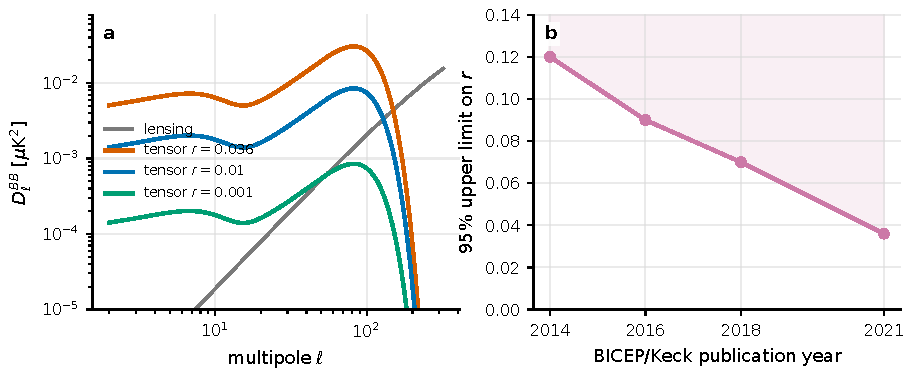
\includegraphics[width=0.9\linewidth]{figures/generated/chapter_16/ch16_bmode_constraints.pdf}
\caption{张量模式主要通过 \(B\) 模偏振受限。左图比较透镜 \(B\) 模与不同 \(r\) 的原初张量 \(B\) 模：\(\ell\sim80\) 的复合峰是地面实验的主战场，低 \(\ell\) 的再电离峰需要大天区。右图显示 BICEP/Keck 系列联合约束从 \(r<0.12\) 一路改进到 \(r_{0.05}<0.036\) 的量级。}
\label{fig:e23-bmode}
\end{figure}

\section{光子穿越宇宙：偏振会被悄悄转过一个角}
\label{sec:e23-birefringence}

前几节都在讲"底片是怎么曝光的"。现在换个视角：光从最后散射面出发，走了近乎整个宇宙的年龄才到我们这里，\textbf{一路上它自己会不会被改写}？第一个可被精密检验的效应，是偏振双折射（cosmic birefringence）——如果存在一种极轻的、像轴子（axion）那样的场耦合到电磁场，光的线偏振方向会在传播中被整体转过一个小角 \(\beta\)。第 \ref{chap:e22} 章从暗物质与轴子的角度写过这种偏振通道；这里我们看它落到 CMB 上会遇到什么麻烦。

麻烦首先是一个\emph{标定}问题。把整片天空的偏振方向转过 \(\beta\)，会让一部分 \(E\) 模泄漏成 \(B\) 模，在 \(EB\)、\(TB\) 这两个本该为零的交叉谱里冒出信号。小角度下这个泄漏近似是
\[
  \frac{C_\ell^{EB}}{C_\ell^{EE}-C_\ell^{BB}}\simeq \tfrac12\tan 4\beta\simeq 2\beta .
\]
代入数字感受量级：\(0.35^\circ=6.1\times10^{-3}\,{\rm rad}\)，于是 \(2\beta\simeq1.2\%\)。这个百分之一的信号，恰好卡在一个尴尬的位置——大到能在 Planck 级全天数据里留下统计迹象，又小到\emph{任何}绝对偏振角标定不准、尘埃自身的 \(EB\)、通带失配或 beam 泄漏都能伪装成它。要命的是，一个真的宇宙旋转角 \(\beta\)，和探测器偏振角整体错标了 \(\alpha\)，在 \(EB/TB\) 里几乎沿同一个方向作用，只用 CMB 你测到的其实是 \(\alpha+\beta\)。分开二者的钥匙，是频率：宇宙学旋转对所有频率一视同仁，而银河前景的偏振随频率变化，探测器错标又是逐频率的仪器量。

Minami 与 Komatsu 正是用这把"频率钥匙"，借银河前景在不同频率上的不同表现，同时估计逐频率的仪器错标 \(\alpha_\nu\) 和宇宙旋转 \(\beta\)，得到 \(\beta=0.35\pm0.14^\circ\)，并把地面角标定约 \(0.28^\circ\) 的系统误差从最终误差里剥离出去。后续用 WMAP+Planck PR4、在 \(23\text{--}353\,{\rm GHz}\) 上加入尘埃 \(EB\) 模型的分析，给出近全天 \(\beta=0.342^{+0.094}_{-0.091}{}^\circ\)，显著性约 \(3.6\sigma\)，但偏振尘埃自身的 \(EB\)、低频同步辐射 \(EB\) 和独立角标定仍是主要限制（图~\ref{fig:e23-biref}）\citep{2020PhRvL.125v1301M,2022PhRvD.106f3503E,2022PhRvL.128i1302D,2022NatRP...4..452K}。若把它解释成轴子样场，旋转角来自场值在传播两端的差：
\begin{equation}
  \beta=\frac12\,g_{\phi\gamma}\,\bigl[\phi(t_0)-\phi(t_{\rm LSS})\bigr] .
  \label{eq:e23-axion-birefringence}
\end{equation}
\begin{formulaexplain}
\(\beta\) 是 CMB 偏振的全局旋转角，\(g_{\phi\gamma}\) 是场与光子的耦合常数，方括号是今天 \(t_0\) 与最后散射面 \(t_{\rm LSS}\) 之间的场值差。若旋转真来自轴子样传播效应，它应\emph{近似不依赖频率}。
\end{formulaexplain}
\(g_{\phi\gamma}\) 的单位是 \({\rm GeV^{-1}}\)，\(\phi\) 是从最后散射面到今天的有效场值。这条式子默认旋转近似各向同性、频率无关、且源自\emph{传播}而非发射面本征的 \(EB\)。反过来，频率依赖就是最好的诊断：若 \(\beta(\nu)\propto\nu^{-2}\)，那更像穿过磁化等离子体的 Faraday 旋转（第 \ref{chap:e21} 章的传播效应）而非轴子；若 \(\beta\) 随天区、红移或时间变化，就得把一个全局角推广成方向依赖或时间依赖的相关函数。这里的教学要点值得记住：\textbf{在宇宙学里，一个"信号"和一个"标定误差"常常长得一模一样，把它们分开靠的往往不是更灵敏的探测器，而是更聪明地利用频率、天区这些额外维度。}

\begin{figure}[tbp]
\centering
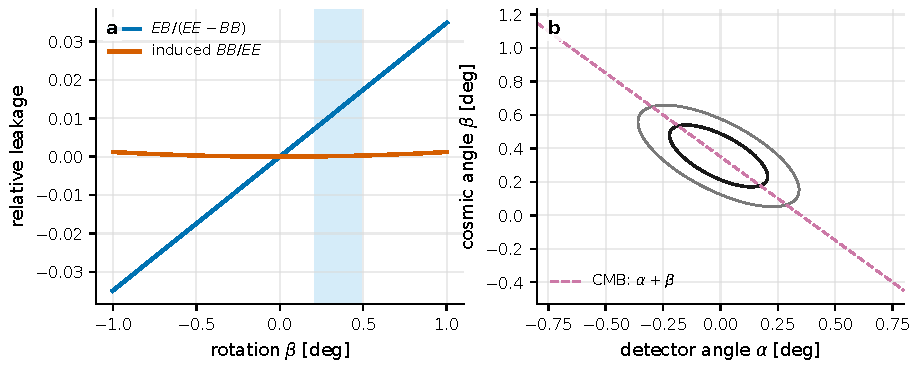
\includegraphics[width=0.9\linewidth]{figures/generated/chapter_16/ch16_birefringence_eb.pdf}
\caption{CMB 双折射把偏振角误差和宇宙学信号放进同一个平面。左图显示 \(\beta\) 对 \(EB\) 和诱导 \(BB\) 的小角度泄漏，阴影标出 \(\beta=0.35\pm0.14^\circ\) 的量级；右图显示探测器角 \(\alpha\) 与宇宙角 \(\beta\) 的退化方向：只用 CMB 时主要测到 \(\alpha+\beta\)，加入前景频率信息才可能把两者分开。}
\label{fig:e23-biref}
\end{figure}

\section{到达时间与色散：用宇宙学基线称量基本物理}
\label{sec:e23-timing}

偏振被转过一个角，是光在路上被改写的一种方式；\textbf{到达时间被拉开}，是另一种。这一节把本书最看重的两件工具——高时间分辨的光子事件表（第 \ref{chap:e13} 章）和瞬变源（第 \ref{chap:e20} 章的快速射电暴、伽马暴、脉冲星）——一起搬到宇宙学基线上，来检验最基本的物理：光速真的和频率无关吗？光子真的严格无质量吗？洛伦兹不变性在极高能量下还成立吗？

思路的核心，是一条比什么都朴素的判据：\textbf{如果一次爆发在同一瞬间发出了各种频率的光，而它们没有同时到达，那么"路上发生了事"}。要把这句话变成可测量，得写下频率与传播速度的关系。先看最熟悉、也最先要扣除的一项——星际与星系际的稀薄等离子体。一束电磁波在冷等离子体里满足的色散关系（dispersion relation）是
\begin{equation}
  \omega^2=\omega_p^2+c^2k^2,
  \qquad
  \omega_p^2=\frac{4\pi n_e e^2}{m_e}.
  \label{eq:e23-plasma-dispersion}
\end{equation}
\begin{formulaexplain}
\(\omega\) 是角频率，\(k\) 是波数，\(\omega_p\) 是等离子体频率，\(n_e\) 是电子数密度，\(e,m_e\) 是电子电荷与质量（CGS 制）。等离子体给色散关系加了一个\emph{常数项} \(\omega_p^2\)，波只有在 \(\omega>\omega_p\) 时才能传播。
\end{formulaexplain}
群速度（信号真正走的速度）是 \(v_g={\rm d}\omega/{\rm d}k\)。从 \eqref{eq:e23-plasma-dispersion} 解出 \(k=\sqrt{\omega^2-\omega_p^2}/c\)，两边对 \(\omega\) 微分再取倒数，一步不跳：
\[
  \frac{{\rm d}k}{{\rm d}\omega}=\frac{1}{c}\frac{\omega}{\sqrt{\omega^2-\omega_p^2}}
  \;\Longrightarrow\;
  v_g=\frac{{\rm d}\omega}{{\rm d}k}=c\,\frac{\sqrt{\omega^2-\omega_p^2}}{\omega}
  =c\sqrt{1-\frac{\omega_p^2}{\omega^2}}
  \simeq c\Bigl(1-\frac{\omega_p^2}{2\omega^2}\Bigr),
\]
最后一步用了 \(\omega_p\ll\omega\) 的泰勒展开 \(\sqrt{1-x}\simeq1-x/2\)。走过路径长度 \(L\) 的时间是 \(t=L/v_g\simeq(L/c)(1+\omega_p^2/2\omega^2)\)。于是两个频率 \(\omega_1<\omega_2\) 同时发出、到达时刻之差为
\begin{equation}
  \Delta t_{\rm plasma}
  =\frac{L}{2c}\,\omega_p^2\Bigl(\frac{1}{\omega_1^2}-\frac{1}{\omega_2^2}\Bigr)
  \;\propto\;\frac{\int n_e\,{\rm d}l}{\nu^2}
  =\frac{\rm DM}{\nu^2}.
  \label{eq:e23-dm-delay}
\end{equation}
\begin{formulaexplain}
\(\Delta t_{\rm plasma}\) 是等离子体色散造成的到达时差，与频率的\emph{平方成反比}，与沿视线积分的电子柱密度 \(\int n_e\,{\rm d}l\)（即色散量 DM，dispersion measure）成正比。低频光走得慢、到得晚。
\end{formulaexplain}
这正是第 \ref{chap:e20} 章里快速射电暴的招牌特征：一个毫秒脉冲在动态谱上被拉成一条 \(\nu^{-2}\) 的弯扫，测出这条弯扫的斜率就得到 DM，反过来还能称出一路上的电子。星际介质里 \(n_e\) 约 \(10^{-2}\text{--}10^{-1}\,{\rm cm^{-3}}\)，星系际更稀薄，但基线一长，柱密度可观，毫秒级的色散延迟稀松平常。

奇妙的是，\textbf{一个有质量的光子会给出结构一模一样的一项}。相对论色散关系是 \(E^2=(pc)^2+(m_\gamma c^2)^2\)——同样是给能量—动量关系加了一个常数项 \((m_\gamma c^2)^2\)，只不过这次是"静能"而不是"等离子体频率"：
\begin{equation}
  E^2=(pc)^2+(m_\gamma c^2)^2 .
  \label{eq:e23-massive-photon}
\end{equation}
\begin{formulaexplain}
\(E=h\nu\) 是光子能量，\(p\) 是动量，\(m_\gamma\) 是假想的光子质量，\(c\) 是（低频极限下的）光速。有质量光子的色散关系，和等离子体那一条在数学上完全同构——把 \(m_\gamma c^2\) 换成 \(\hbar\omega_p\) 就重合了。
\end{formulaexplain}
照搬上面的群速度推导（\(E\) 对应 \(\hbar\omega\)，\(p\) 对应 \(\hbar k\)）：\(v_g=\partial E/\partial p=pc^2/E=c\sqrt{1-(m_\gamma c^2/E)^2}\simeq c\,[1-\tfrac12(m_\gamma c^2/E)^2]\)，于是两个能量的到达时差是
\[
  \Delta t_{m_\gamma}=\frac{L}{2c}\,(m_\gamma c^2)^2\Bigl(\frac{1}{E_1^2}-\frac{1}{E_2^2}\Bigr)
  \;\propto\;\frac{1}{\nu^2}.
\]
它和等离子体延迟一样按 \(\nu^{-2}\) 走——这既是好消息也是坏消息。好消息：任何能测色散延迟的手段（射电脉冲星、快速射电暴）天生就能给 \(m_\gamma\) 定上限。坏消息：光子质量与等离子体的延迟\emph{完全退化}，必须靠独立测定的 DM（比如多条视线、多个源）把等离子体那份先扣干净，剩下的才可能归给 \(m_\gamma\)。判据依旧朴素：一次跨越宇宙学距离的爆发，若不同频率的主脉冲在扣除已知 DM 后仍\emph{一致到极高精度}，就把 \(m_\gamma\) 逼到极小的上限——基线 \(L\) 越长、时间分辨越细、频率跨度越大，这把尺子越狠。

第三种可能，藏在更高的能量里。若洛伦兹不变性在接近某个量子引力能标 \(E_{\rm QG}\) 时被极微弱地破坏（Lorentz invariance violation，LIV），色散关系会多出一个\emph{随能量增长}的修正项：
\begin{equation}
  E^2\simeq p^2c^2\Bigl[\,1\pm\Bigl(\frac{E}{E_{\rm QG}}\Bigr)^{n}\Bigr],
  \label{eq:e23-liv-dispersion}
\end{equation}
\begin{formulaexplain}
\(E_{\rm QG}\) 是洛伦兹破缺可能出现的能标（常拿普朗克能标当参照），\(n\) 是修正的幂次（\(n=1\) 线性、\(n=2\) 二次），\(\pm\) 表示高能光子可能走得更快或更慢。它与质量项的关键区别是：修正随能量\emph{升}高而变强。
\end{formulaexplain}
把 \eqref{eq:e23-liv-dispersion} 解出 \(p\simeq(E/c)[1\mp\tfrac12(E/E_{\rm QG})^n]\)，再取群速度 \(v=\partial E/\partial p\simeq c\,[1\pm\tfrac{n+1}{2}(E/E_{\rm QG})^n]\)，得到到达时差
\[
  \Delta t_{\rm LIV}\simeq\pm\,\frac{L}{c}\,\frac{n+1}{2}\,\frac{E_2^{\,n}-E_1^{\,n}}{E_{\rm QG}^{\,n}} .
\]
注意它的频率依赖和前两者\emph{正好相反}：等离子体和光子质量让\emph{低}频拖后腿（\(\propto\nu^{-2}\)），LIV 则让\emph{高}能光子领先或落后（\(\propto E^{n}\)）。这个符号与幂次上的差别，就是把三种效应拆开的抓手。所以检验 LIV 的天然对象是伽马暴和高能爆发：它们同时抛出低能与极高能光子，又在宇宙学距离外，\(L\) 与 \(\Delta E\) 都被拉到极致；只要在事件表里精确记下每个高能光子的到达时刻，再和低能光子对齐，就能把 \(E_{\rm QG}\) 顶到很高的下限。

把三条延迟并排看，本章的方法论就浮出来了（表~\ref{tab:e23-delays} 的口味）：同一套"高时间分辨事件表 + 宇宙学长基线"的观测，喂给三种不同频率依赖的模型，就能分别称量介质、光子质量与时空本身。这里我们不引用任何具体的数值上限——那属于实验前沿、且与选源和建模强相关；本节要教给你的是\emph{思路}：宇宙学距离不是障碍，它是把最微弱的基本物理效应\emph{放大}成可测到达时差的免费杠杆。第 \ref{chap:e13} 章那句"把每个光子的时间标签留在事件表里"，到这里终于显出它最大的野心——那根时间轴，长到可以量一量光子有没有质量、时空是不是严格洛伦兹不变。

\begin{table}[tbp]
\centering
\caption{三种到达时差的频率依赖各不相同，这正是把它们分开的抓手。}
\label{tab:e23-delays}
\begin{tabular}{@{}lll@{}}
\toprule
效应 & 色散关系里的多出项 & 到达时差随频率\\
\midrule
等离子体色散 & \(+\,\omega_p^2\)（\(\propto n_e\)） & \(\Delta t\propto \nu^{-2}\)，低频晚到\\
光子质量 & \(+\,(m_\gamma c^2)^2\) & \(\Delta t\propto \nu^{-2}\)，低频晚到（与等离子体退化）\\
洛伦兹破缺 & \(\pm\,p^2c^2(E/E_{\rm QG})^n\) & \(\Delta t\propto E^{n}\)，高能领先或落后\\
\bottomrule
\end{tabular}
\end{table}

顺带说一句相干性。到达时间被拉开的另一面，是相位记忆被打乱。第 \ref{chap:e02} 章讲过，一束光"还记得自己相位"的时间是相干时间 \(\tau_c\simeq1/\Delta\nu\)。当光穿过湍动的星际/星系际等离子体，多条略有不同的路径会让脉冲展宽、让相位在到达时被搅散，等效于把相干性磨损掉一部分——这正是第 \ref{chap:e21} 章传播效应要细算的散射。对本章而言，只需记住一个方向性的结论：\textbf{宇宙学距离既是放大微弱物理的杠杆，也是消磨相干与展宽脉冲的介质}；一台想在宇宙学基线上做精密计时或相干测量的仪器，必须同时把这两面写进它的误差预算（第 \ref{chap:e15} 章）。

\section{CMB 与光学量子天文学如何对接}
\label{sec:e23-bridge}

最后把这一章缝回全书。CMB 和前几部分的光学量子天文学，共享同一套"相关函数"的语言，但观测的含义天差地别——认清这个差别，才不会把两边的"量子"随手互换。

本书前半程反复用二阶相干函数 \(g^{(2)}\) 去刻画探测器时间序列里的强度涨落（第 \ref{chap:e08}、\ref{chap:e10} 章）：
\[
  g^{(2)}(\tau)=\frac{\langle I(t)\,I(t+\tau)\rangle}{\langle I\rangle^2}.
\]
它的时间延迟 \(\tau\) 和带宽 \(\Delta\nu\)，都是你可以\emph{主动挑}的。CMB 的基本二点函数则活在天球上，模式数由宇宙一次性发好：
\begin{equation}
  \langle X_{\ell m}\,Y^*_{\ell'm'}\rangle=C_\ell^{XY}\,\delta_{\ell\ell'}\,\delta_{mm'},
  \qquad
  X,Y\in\{T,E,B,\phi_{\rm lens}\}.
  \label{eq:e23-cmb-correlator}
\end{equation}
\begin{formulaexplain}
\(C_\ell^{XY}\) 是两个天空场 \(X,Y\) 的角功率谱，两个 Kronecker delta 表示在各向同性天空里不同 \(\ell,m\) 模式互不相关。这就是 CMB 版的二点相关函数。
\end{formulaexplain}
对照着读：\(g^{(2)}\) 的 \(\tau\) 与 \(\Delta\nu\) 由仪器主动设定，你可以换个延迟、换个带宽再测一遍；\(C_\ell\) 的模式数由宇宙给定，观测者只能改 sky mask、频率组合、beam、噪声权重和前景模型。CMB 没法像实验室那样调制源、重制备初态、重跑一次——它给的是早期场模式的统计信息，投影在 \(T/E/B\)、透镜与更高阶相关里的一份影子。

真正把这份影子变成宇宙学数字的，是地图级（map-level）的似然。所有频率图、偏振图和外部示踪都汇进同一个数据向量 \(\bm d\)：
\begin{equation}
  \bm d=\bm P\,[\,\bm s_{\rm CMB}(\bm\theta)+\bm s_{\rm fg}(\bm\eta)\,]+\bm n,
  \qquad
  -2\ln\mathcal L=(\bm d-\bm m)^{\mathsf T}\,C^{-1}\,(\bm d-\bm m)+\ln\det C .
  \label{eq:e23-cmb-likelihood}
\end{equation}
\begin{formulaexplain}
\(\bm d\) 是地图级数据向量，\(\bm P\) 是含 beam、mask、扫描策略与通带的观测/制图算子，\(\bm s_{\rm CMB}\)、\(\bm s_{\rm fg}\) 是宇宙信号与前景，\(\bm n\) 是噪声。似然把模型残差和总协方差 \(C\) 放在一起，就是从天空图推断宇宙学参数的工作形式。
\end{formulaexplain}
其中 \(\bm\theta\) 是宇宙学参数（如 \(A_s,n_s,\Omega_bh^2,\Omega_ch^2,r,\beta\)），\(\bm\eta\) 是前景参数（尘埃温度与谱指数、同步辐射谱指数、空间去相关等），协方差 \(C\) 一口气装下仪器噪声、样本方差、前景残差与校准不确定性。Planck、Simons Observatory 以及未来 CMB-S4、LiteBIRD 类实验的差别，主要就体现在 \(\bm P\)、\(C\)、频率覆盖、角分辨率和可控系统误差上 \citep{2016A&A...594A..13P,2016A&A...594A..20P,2017MNRAS.472.1195C,2019JCAP...02..056A,2020A&A...641A...6P}。

读 CMB 文献时，单位和 pivot 最坑人，临别叮嘱三句。其一，\(T_0\) 是 K，涨落图常用 \(\mu{\rm K}\)，而原初 \(\mathcal P_{\mathcal R}\) 无量纲——\(A_s\sim2.1\times10^{-9}\) 不能直接和 \(D_\ell^{TT}\sim5000\,\mu{\rm K}^2\) 比，中间隔着一整个辐射转移函数。其二，\(k\)（单位 \({\rm Mpc^{-1}}\)）和 \(\ell\)（角向模式数）通过 \(\ell\simeq k\,D_A(z_*)\) 相联，\(D_A(z_*)\) 是最后散射面的共动角直径距离。其三，\(r\) 的 pivot 不统一，\(r_{0.002}\) 和 \(r_{0.05}\) 不是同一个数，放开 \(n_t\) 时尤其不能混用。第 \ref{chap:e24} 章的量子网络望远镜会把讨论带回可以主动操控的实验系统；CMB 则站在相反的极限——初态不可重做，光路不可重置，可它把早期宇宙那场量子涨落留下的统计痕迹，工工整整地印在了一张我们今天才读到的底片上。

\section*{本章要点}
\addcontentsline{toc}{section}{本章要点}

\begin{itemize}
\item \textbf{CMB 首先是一个光场。} 平均是 \(T_0=2.7255\,{\rm K}\) 的黑体，信息在其上 \(\Delta T/T\sim10^{-5}\) 的角向涨落和偏振里；角功率谱 \(C_\ell\) 是核心二点统计，而低 \(\ell\) 有躲不掉的宇宙方差 \(\sqrt{2/[(2\ell+1)f_{\rm sky}]}\)。
\item \textbf{原初涨落的种子是量子的。} 暴胀把每个模式当成时变频率谐振子，出视界后曲率扰动被冻结；用量子光学语言，这是 \(\bm k\) 与 \(-\bm k\) 的两模压缩态，固定相位解释了成串的声学峰。
\item \textbf{退相干把量子变经典。} 与环境纠缠让约化密度矩阵的非对角项被 \(\exp[-\Gamma_k(q-q')^2]\) 压死，当 \(\Gamma_k(\Delta q)^2\gg1\)，功率谱就可按经典随机场计算——这就是"量子涨落变成经典密度扰动"的确切含义。
\item \textbf{高阶统计与张量模检验"怎样产生"。} \(f_{\rm NL}\) 与零相容，支持最简单场慢滚；\(r_{0.05}<0.036\) 把原初引力波（那位偏振里的 \(B\) 模稀客）压到能标 \(\lesssim1.6\times10^{16}\,{\rm GeV}\)，难点在于扣除透镜与尘埃。
\item \textbf{光在路上会被改写。} 偏振可能被转过 \(\beta\sim0.3^\circ\)（双折射），分离宇宙角与仪器角靠的是频率维度；到达时间可能被拉开，等离子体与光子质量给 \(\nu^{-2}\) 延迟且彼此退化，洛伦兹破缺给 \(E^{n}\) 延迟——频率依赖的不同，正是拆开它们的抓手。
\item \textbf{宇宙学距离是免费的杠杆。} 高时间分辨事件表（第 \ref{chap:e13} 章）配上宇宙学长基线与瞬变源，可把光子质量与洛伦兹破缺等最微弱的效应放大成可测的到达时差——代价是同一段距离也会消磨相干、展宽脉冲。
\end{itemize}

\medskip
\noindent\textbf{想一想。}
\begin{enumerate}
\item 全天 \(\ell=2\) 的宇宙方差相对误差约 \(63\%\)。若只观测半个天空（\(f_{\rm sky}=0.5\)），这个误差变成多少？为什么再灵敏的探测器也补不回这部分信息？
\item 等离子体色散和光子质量都给出 \(\nu^{-2}\) 的到达延迟。如果你手上有\emph{同一批}射电爆发在\emph{不同视线方向}的数据，你会怎样利用 DM 的变化，把可能的光子质量那一份从等离子体里剥出来？
\item 一个真实的宇宙偏振旋转 \(\beta\) 和探测器角错标 \(\alpha\)，在 CMB 里都表现为 \(EB\) 信号。为什么"用不同频率的前景"能把二者分开，而"把探测器做得更灵敏"不能？
\end{enumerate}


% ============================================================
\part{前沿、案例与实践}
\chapter{量子网络望远镜}
\label{chap:e24}

\begin{chapteropening}
第 \ref{chap:e09} 章我们学会了把两台望远镜的光合到一起、数条纹：条纹的可见度就是复可见度 \(V\)，而 \(V\) 藏着恒星的角结构。可那一章也留下一个沉重的脚注——要让条纹稳定，两条光路的光程差必须锁在远小于一个波长的精度上，而且任何一路上的损耗都会\emph{直接吞掉本就稀少的星光光子}。基线拉到几公里、几十公里，这两条要求就双双失控。本章要问一个大胆的问题：能不能\emph{不把未知的星光长途搬运}，却仍然把两台相隔很远的望远镜"接成一台"？答案来自量子信息：预先制备好、可以验证、失败还能重来的\textbf{纠缠资源}（entanglement resource），加上\textbf{量子存储}（quantum memory）与\textbf{量子中继}（quantum repeater），让两端"共享"一个单光子的相位关系，而不必让那个脆弱的星光光子亲自跑完全程。这条路线目前还不是一台成熟的仪器，而是一张需要一项项算清的可行性账本；本章就带你把这张账本从头搭起来，并和第 \ref{chap:e10} 章的强度干涉摆在一起对照。
\end{chapteropening}

\section{为什么长基线的振幅干涉被光子损耗掐住}
\label{sec:e24-why-loss}

先把问题剥到最小。我们真正想保住的，不是"更多的光"，而是\emph{一阶相干的那个相位}。设想天空里一个点源，在一个相干时间 \(\tau_c\simeq1/\Delta\nu\)（第 \ref{chap:e02} 章）的时间窗里，恰好有一个来自它的光子飞到望远镜阵。极弱星光的关键事实是：每个时间窗里来自天体的平均光子数 \(\epsilon\ll1\)，绝大多数窗口是空的，偶尔一个窗口里只有一个光子。这一个光子，如果在到达探测器之前没有被"它究竟走了哪条路"这种信息污染，它就\emph{不是}"已经属于左望远镜"或"已经属于右望远镜"的经典粒子，而是左、右两条接收路径的量子叠加：

\begin{equation}
  |\psi_\star\rangle
  =
  \frac{|1\rangle_L|0\rangle_R
  +
  e^{i\phi}\,|0\rangle_L|1\rangle_R}{\sqrt2},
  \qquad
  \phi=\frac{2\pi\,\bm{B}\cdot\bm{\theta}}{\lambda}.
  \label{eq:e24-stellar-single-photon}
\end{equation}
\begin{formulaexplain}
\(|\psi_\star\rangle\) 是一个星光光子在左右两孔径之间的路径叠加态；\(|1\rangle_L|0\rangle_R\) 表示"左边有一个光子、右边为空"，另一项相反。\(\phi\) 是由基线 \(\bm{B}\)、源角位置 \(\bm{\theta}\) 与波长 \(\lambda\) 定出的几何相位。振幅干涉要保住的正是这个 \(\phi\)。
\end{formulaexplain}

这里 \(|1\rangle_L|0\rangle_R\) 是数态记号（第 \ref{chap:e05} 章）：下标 \(L,R\) 标记左、右两个空间模式，括号里的数字是该模式的光子数。\(\bm{B}\) 是投影基线（单位 cm，量级从 \(10^2\,\mathrm{cm}\) 到 \(10^7\,\mathrm{cm}\)），\(\bm{\theta}\) 是点源相对相位中心的角位置（无量纲弧度），\(\lambda\) 是波长（可见光 \(\sim6\times10^{-5}\,\mathrm{cm}\)）。相位 \(\phi\) 无量纲，是纯几何量——它就是第 \ref{chap:e09} 章条纹里的那个相位，只不过现在写成了单光子叠加态的语言。

真实恒星不是点，而是许多互不相干的点源之和（这正是第 \ref{chap:e10} 章 van Cittert--Zernike 定理的出发点）。每个子源 \(j\) 各自给出一个相位 \(\phi_j\) 的纯态 \eqref{eq:e24-stellar-single-photon}，非相干叠加就是把这些纯态按亮度加权求和成一个混合态；求和后，非对角元里出现的正是那些相位因子的加权平均 \(\langle e^{i(\phi_j-\phi_k)}\rangle\)，它恰好收敛成第 \ref{chap:e10} 章那个复可见度 \(V\)。只看单光子子空间 \(\{|10\rangle,|01\rangle\}\)，它的密度矩阵是

\begin{equation}
  \rho_1
  =
  \frac{1}{2}
  \begin{pmatrix}
  1 & V\\[2pt]
  V^* & 1
  \end{pmatrix}_{\{|10\rangle,\,|01\rangle\}} ,
  \qquad
  V=|V|\,e^{i\arg V}.
  \label{eq:e24-single-photon-density}
\end{equation}
\begin{formulaexplain}
\(\rho_1\) 是单光子子空间的密度矩阵；对角元 \(\tfrac12\) 只说明"光子可在任一台望远镜出现"，非对角元 \(V\) 才是复可见度，装着源的相干相位和角结构。\(|V|\) 从 1（点源）降到 0（源大到解析开），相位则给出源的位置与不对称。
\end{formulaexplain}

请对照第 \ref{chap:e10} 章式 \eqref{eq:e10-gamma12}：那里的复可见度 \(\gamma^{(1)}_{12}\) 是用两路场的时间平均定义的，这里的 \(V\) 就是同一个量，只是搬进了单光子密度矩阵的非对角元。物理含义完全一致：\emph{把 \(V\) 测出来，就等于测到了恒星}。传统振幅干涉的做法，是把 \(L,R\) 两个空间模式用光纤或自由空间光路送到\emph{同一个}合束器（beamsplitter）上，让 \(\phi\) 变成可数的条纹。麻烦就出在"送到同一个合束器"这一步：其中一路若走过长度 \(L\) 的有损链路，单光子透过率是

\begin{equation}
  \eta_{\rm ch}(L)=10^{-\alpha_{\rm dB}L/10}.
  \label{eq:e24-link-loss}
\end{equation}
\begin{formulaexplain}
\(\eta_{\rm ch}\) 是链路透过率（无量纲，\(0\) 到 \(1\)）；\(\alpha_{\rm dB}\) 是每公里的分贝损耗（单位 \(\mathrm{dB\,km^{-1}}\)），\(L\) 是链路长度（km）。分贝损耗让透过率随距离\emph{指数}衰减——这就是长基线直接光学合束的核心瓶颈。
\end{formulaexplain}

分贝是个对数刻度：\(10\,\mathrm{dB}\) 表示衰减到 \(1/10\)，\(20\,\mathrm{dB}\) 表示 \(1/100\)。把真实数字代进去感受一下。可见光在普通光纤里的损耗高达 \(20\)–\(30\,\mathrm{dB\,km^{-1}}\)，走 \(1\,\mathrm{km}\) 就只剩 \(10^{-2}\) 到 \(10^{-3}\) 以下——本就 \(\epsilon\ll1\) 的星光，几乎被吃干净。换到 \(1550\,\mathrm{nm}\) 的电信波段（telecom band），最好的光纤能低到 \(\sim0.2\,\mathrm{dB\,km^{-1}}\)，可星光并不天生长在这个波段，要先做频率转换、耦合、相位稳定，每一步都再乘一个小于 1 的效率；晴空自由空间链路可用 \(\sim0.5\,\mathrm{dB\,km^{-1}}\) 做量级估算，但大气湍流和指向误差带来的损失并不是这条干净的指数律 \citep{2012PhRvL.109g0503G,2019PhRvL.123g0504K,2024SPIE13095E..1NR}。一句话：\emph{你越想拉长基线，就越要把这个本来就稀缺的星光光子送得更远，而它被丢掉的概率随距离指数上升}。

\begin{figure}[tbp]
\centering
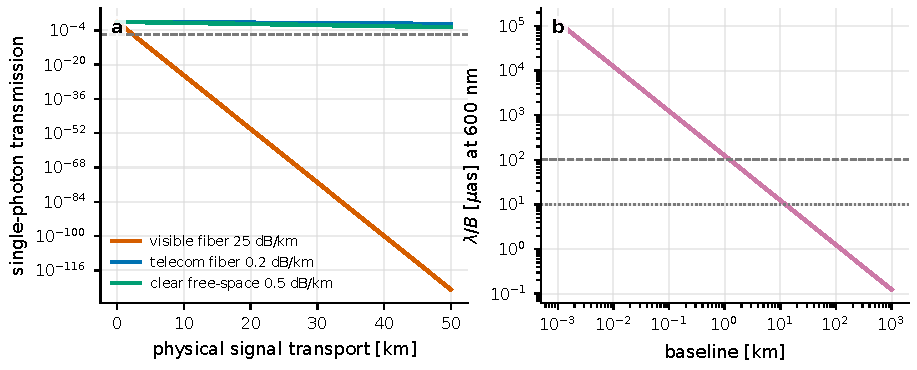
\includegraphics[width=0.94\linewidth]{figures/generated/chapter_17/ch17_architecture_loss.pdf}
\caption{长基线的诱惑与困难来自同一个量纲。左图把"直接传输单光子星光"的几种链路损耗画成透过率：可见光光纤在公里尺度就已严重衰减，电信波段光纤也会在百公里尺度变得昂贵。右图给出角分辨率标度 \(\lambda/B\)：\(600\,\mathrm{nm}\) 的光在 \(1\,\mathrm{km}\) 基线上达到百微角秒量级，\(100\,\mathrm{km}\) 基线进入微角秒量级。}
\label{fig:e24-architecture-loss}
\end{figure}

那为什么还要费这么大劲拉长基线？因为角分辨率的基本标度只认基线长度 \(B\)：

\begin{equation}
  \theta_{\rm res}\sim\frac{\lambda}{B}
  =124\,\mu\mathrm{as}
  \left(\frac{\lambda}{600\,\mathrm{nm}}\right)
  \left(\frac{1\,\mathrm{km}}{B}\right).
  \label{eq:e24-resolution-scale}
\end{equation}
\begin{formulaexplain}
\(\theta_{\rm res}\) 是干涉的角分辨率标度（这里用微角秒 \(\mu\mathrm{as}\)），\(B\) 是基线长度。基线越长，能分辨的角结构越细。量子网络方案追求的，正是在\emph{不长途搬运未知星光}的前提下，把 \(B\) 推到公里乃至更远。
\end{formulaexplain}

把括号里的比值代成 1，就读出 \(124\,\mu\mathrm{as}\) 这个基准；\(B=10\,\mathrm{km}\) 给 \(12\,\mu\mathrm{as}\)，\(B=100\,\mathrm{km}\) 给 \(1.2\,\mu\mathrm{as}\)。作为参照，最大的光学干涉阵列（如 CHARA）基线约几百米，只能到毫角秒级。量子网络望远镜的吸引力就锁在这个尺度上：它未必提高单孔径的灵敏度，却可能把光学/近红外干涉从几百米一路推向公里、十公里甚至更长。第 \ref{chap:e10} 章的强度干涉（HBT）其实早就绕开了光程传输这道坎——它不合束、只在本地记录强度涨落再离线相关，因此几乎不怕大气抖动，代价是它主要给 \(|V|^2\)，把相位丢了。量子网络路线的野心不同：它想\emph{保住一阶相干的相位}，同时又\emph{不把未知星光搬运长途}。

\section{预共享纠缠：把要长途搬运的东西换掉}
\label{sec:e24-gjc}

核心的一招，Gottesman--Jennewein--Croke 想出来了：既然长途搬运脆弱的未知星光如此昂贵，那就\emph{别搬它}，改搬一个我们完全掌握、可以验证、坏了还能重做的"实验室光子"。这个实验室光子被预先制备成一个已知的路径纠缠态：

\begin{equation}
  |\Phi_\delta\rangle
  =
  \frac{|1\rangle_L|0\rangle_R
  +
  e^{i\delta}\,|0\rangle_L|1\rangle_R}{\sqrt2}.
  \label{eq:e24-lab-entangled-photon}
\end{equation}
\begin{formulaexplain}
\(|\Phi_\delta\rangle\) 是预共享的实验室路径纠缠光子，形式和星光态 \eqref{eq:e24-stellar-single-photon} 一模一样，只是相位 \(\delta\) 完全由我们掌控。它替代了"长途搬运未知星光"的任务：这份纠缠可以提前分发、事后验证，失败就丢弃重来，绝不动用宝贵的星光。
\end{formulaexplain}

注意 \(|\Phi_\delta\rangle\) 和 \(|\psi_\star\rangle\) 的结构惊人地相似——都是"左有一个 / 右有一个"的叠加，差别只是相位一个是天定的 \(\phi\)、一个是人定的 \(\delta\)。这就是全部窍门：让\emph{已知的} \(\delta\) 去和\emph{未知的} \(\phi\) 做本地干涉，从而把 \(\phi\)（也就是 \(V\)）读出来，而两端都不必把自己的光子送到对方那里。

具体怎么读？星光光子到达后，左、右两站各自\emph{在本地}把"星光模式"和"实验室纠缠模式"一起送进一个合束器，然后只保留"左站探到一个光子、右站也探到一个光子"这类特定的符合（coincidence）事件。合束器的作用和第 \ref{chap:e09} 章一样：它把两路输入振幅线性组合成 \((\text{星光}\pm\text{实验室})/\sqrt2\) 两个输出端，于是每个输出端的场都成了两条路径振幅的\emph{相干叠加}。做完这一步，"这个光子究竟是星光还是实验室光、走的哪条路"这类\emph{路径信息被擦除}，留下的只有两条路径之间的相位关系 \(\phi-\delta\)。左右两端各触发一次的符合概率，正比于这两条被擦除路径振幅相干叠加后的模方；把星光态 \eqref{eq:e24-stellar-single-photon} 与实验室态 \eqref{eq:e24-lab-entangled-photon} 代进去展开，模方里的\emph{交叉项}恰好是 \(\mathrm{Re}(V e^{-i\delta})\)——这正是干涉信息的载体。完整的两模合束器加符合代数在量子光学教科书里是标准结果，这里直接给出它的结论：相关与反相关两类符合点击的概率是

\begin{equation}
  P_{\pm}(\delta)
  =
  \frac{1}{2}
  \Bigl[\,1\pm\mathrm{Re}\!\left(V\,e^{-i\delta}\right)\Bigr].
  \label{eq:e24-gjc-probability}
\end{equation}
\begin{formulaexplain}
\(P_\pm(\delta)\) 是两类符合点击的概率，\(V\) 是星光复可见度，\(\delta\) 是我们可调的实验室相位。改变 \(\delta\) 就像扫描一个参考相位：点击率会随 \(\delta\) 正弦式振荡，从振荡的幅度和相位就能读出 \(V\) 的实部与虚部。
\end{formulaexplain}

把 \(V=|V|e^{i\arg V}\) 代进去，\(\mathrm{Re}(Ve^{-i\delta})=|V|\cos(\arg V-\delta)\)，于是 \(P_\pm(\delta)\) 随 \(\delta\) 上下起伏的\emph{振荡深度}正是 \(|V|\)，\emph{相位}正是 \(\arg V\)。换句话说，扫一遍 \(\delta\)，就把复可见度整个测了出来——和第 \ref{chap:e09} 章扫描光程差得到条纹是完全一样的物理，只不过参考相位现在由本地的纠缠资源提供，星光光子从头到尾没离开过自己那一站。这里的"本地合束器 + 符合探测"在量子信息里叫\textbf{贝尔态测量}（Bell-state measurement）：把两个光子投影到一组最大纠缠的两模基上。可惜线性光学只能无歧义地分辨其中一部分点击组合，所以只有大约一半的有效星光事件能进入估计；若能做完整的贝尔态测量或更复杂的量子处理，这 \(50\%\) 的损失原则上可以避免 \citep{1982Natur.299..802W,1993PhRvL..70.1895B,2012PhRvL.109g0503G}。

问题也随之而来，而且很硬——\textbf{资源率}。这条直接的 GJC 路线要求：\emph{每一个可能装着星光的相干时间窗，都得预先备好一个匹配的纠缠光子}。带宽 \(\Delta\nu\) 决定相干时间约 \(1/\Delta\nu\)，于是每秒要覆盖的时间窗数约为 \(\Delta\nu\)。取 \(\Delta\nu=10\,\mathrm{GHz}\)，就是每秒 \(10^{10}\) 个窗口——也就是说，你得有一台每秒吐出 \(10^{10}\) 个高质量纠缠光子对的源。天文路线图（Rajagopal 等）明确指出，当前最好的纠缠光子源速率离这个数还差得很远；因此直接 GJC 更适合作为\emph{短基线的上天原理验证}，短期内还难以取代现有的光学干涉阵列 \citep{2024SPIE13095E..1NR,2012PhRvL.109g0503G}。

Khabiboulline--Borregaard--De Greve--Lukin 的方案巧妙地反过来利用"星光很弱"这件事。既然每个长测量窗口里平均只有 \(\epsilon\ll1\) 个相关星光光子，就把窗口切成 \(M\sim1/\epsilon\) 个更细的时间小格（time bin），那么\emph{至多只有一个小格里真有光子}。要记住"光子落在了哪个小格"，笨办法（unary code，一位一格）要 \(M\) 个纠缠对；聪明办法（binary code，用二进制编码到达时间）只需要

\begin{equation}
  n_{\rm mem}
  =
  \bigl\lceil\log_2(M+1)\bigr\rceil
  \simeq
  \bigl\lceil\log_2(1/\epsilon)\bigr\rceil
  \label{eq:e24-binary-timebin}
\end{equation}
\begin{formulaexplain}
\(n_{\rm mem}\) 是需要的存储量子比特（qubit）数，\(M\) 是时间小格数，\(\epsilon\) 是每格平均星光光子数。弱光的\emph{稀疏性}把资源需求从 \(M\) 个纠缠对压到约 \(\log_2 M\) 个存储位——这是指数级的节省。
\end{formulaexplain}

个存储 qubit，每一位用一个纠缠对做一次非局域的\textbf{宇称校验}（parity check）。数量级立刻变得诱人：若 \(M=10^6\)，只需约 \(20\) 个 qubit 就能编码到达时间，而 unary code 要一百万个纠缠对。论文给出的代表性算例是：对带宽 \(\Delta f=1\,\mathrm{MHz}\)、\(1\,\mathrm{s}\) 的测量窗口，\(N=10^6\) 个时间小格对应 \(\log_2 N\simeq20\) 个 qubit；在一个天文例子里，\(10\) 等星、\(10\,\mathrm{m^2}\) 收集面积、\(10\,\mathrm{GHz}\) 检测带宽，推出的资源目标约是 \(20\)–\(30\) 个 qubit 加上 \(\sim200\,\mathrm{kHz}\) 的纠缠供应率。Stas 等的补充分析也用 \(20\) 个 SiV 节点、\(1\,\mathrm{kHz}\) 的零距离纠缠率和 \(1\,\mathrm{s}\) 窗口，演示了这种对数缩放的可行路径 \citep{2019PhRvL.123g0504K,2022PhRvA.106c2424C,2026Natur.651..326S,2024SPIE13095E..1NR}。

\begin{figure}[tbp]
\centering
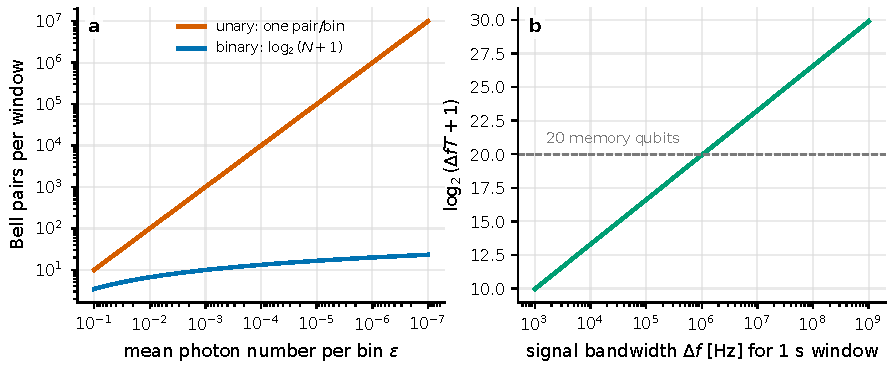
\includegraphics[width=0.94\linewidth]{figures/generated/chapter_17/ch17_timebin_scaling.pdf}
\caption{正是"星光很弱"让时间小格编码有意义。左图比较 unary 与 binary 两种编码对纠缠对的需求：当每格平均光子数 \(\epsilon\) 很小，\(M\sim1/\epsilon\) 个小格可以只用 \(\log_2(M+1)\) 个存储 qubit 来标记。右图显示 \(1\,\mathrm{s}\) 测量窗口里，\(1\,\mathrm{MHz}\) 带宽对应约 \(10^6\) 个小格，也就是约 \(20\) 个 qubit。}
\label{fig:e24-timebin}
\end{figure}

支撑这一切的底层通信技术，是\textbf{量子中继}。为什么不能像放大电信号那样，把量子态放大着往远处传？因为\emph{不可克隆定理}（no-cloning theorem）禁止完美复制一个未知量子态 \citep{1982Natur.299..802W}，而损耗又随距离指数上升（式 \eqref{eq:e24-link-loss}）。中继的思路是分而治之：把长距离切成许多短段，先在每一短段内建立纠缠（短段损耗小、成功率高），再用\textbf{纠缠交换}（entanglement swapping）把相邻短段的纠缠"接龙"成跨越全程的纠缠。理想的中继能把指数损耗换成温和得多的资源缩放，但真实系统还要面对贝尔态测量的成功率、存储寿命、暗计数、门保真度和频率转换等一连串折损。DLCZ 原子系综协议、量子互联网路线以及量子存储综述，都把\emph{存储}放在资源预算的正中央——因为存储的职责，是把这些概率性成功的事件在时间上\emph{对齐}起来 \citep{1998PhRvL..81.5932B,2001Natur.414..413D,2011RvMP...83...33S,2008Natur.453.1023K,2012IEEEN..26d..59V,2006quant.ph..7182U}。

\section{资源账本：纠缠率、存储时间、保真度怎样一起闭合}
\label{sec:e24-budget}

无论上面哪个方案，最后都要回到同一张账本。角分辨率由 \(B\) 白送（式 \eqref{eq:e24-resolution-scale}），可\emph{能不能真的观测}，却要纠缠供应率、存储时间、保真度和星光事件率四项\emph{同时}达标；缺一项，长基线那根相位杠杆就撬不动。

第一项是\textbf{纠缠供应率}。设被接受的有效星光事件率是 \(R_\star\)，每个事件平均消耗 \(n_{\rm pair}\) 个纠缠对，那么

\begin{equation}
  R_{\rm ent}
  \gtrsim
  \frac{n_{\rm pair}\,R_\star}{p_{\rm ready}} .
  \label{eq:e24-entanglement-rate}
\end{equation}
\begin{formulaexplain}
\(R_{\rm ent}\) 是所需的纠缠供应率（单位 Hz），\(R_\star\) 是有效星光事件率（Hz），\(n_{\rm pair}\) 是每个事件消耗的纠缠对数，\(p_{\rm ready}\) 是星光到达时纠缠对已备好的概率。它把天文事件率\emph{直接翻译}成量子网络的吞吐量要求。
\end{formulaexplain}

要读懂这条式子，得先把 \(R_\star\) 讲清楚：它\emph{不是}望远镜收到的总光子率，而是进入了目标空间模式、频率通道、偏振通道、时间窗，并通过质量筛选之后，\emph{真正能用}的事件率。\(p_{\rm ready}\) 越接近 1，说明纠缠资源几乎总是待命，浪费越少。这条式子的启示很直接：对又亮又宽带的源，\(R_\star\) 极高，直接 GJC 会被资源率活活压垮；对又窄带又暗弱的源，\(R_\star\) 小，存储辅助方案才有机会用一个较低的 \(R_{\rm ent}\) 去换取长基线。

第二项是\textbf{存储时间}。最起码，量子态或测量记录要一直存到经典通信和非局域校验都完成为止：

\begin{equation}
  T_{\rm mem}
  \gtrsim
  \max\!\left[\frac{B}{c},\,T_{\rm ent},\,T_{\rm proc},\,T_{\rm win}\right].
  \label{eq:e24-memory-time}
\end{equation}
\begin{formulaexplain}
\(T_{\rm mem}\) 是量子存储必须保持相干的最短时间，等于右边四项取最大：基线光行时 \(B/c\)、纠缠生成时间 \(T_{\rm ent}\)、处理时间 \(T_{\rm proc}\)、测量窗口 \(T_{\rm win}\)。真正卡脖子的往往\emph{不是} \(B/c\)，而是同步和时间小格窗口。
\end{formulaexplain}

代个数字就明白了：光行时 \(B/c=3.3\,\mu\mathrm{s}\times(B/\mathrm{km})\)，所以 \(100\,\mathrm{km}\) 基线只要 \(0.33\,\mathrm{ms}\) 的光行时——听起来很轻松。可 Khabiboulline 型的二进制时间小格方案，为了覆盖窄带弱光，测量窗口 \(T_{\rm win}\) 可能长达 \(\sim1\,\mathrm{s}\)，比光行时严苛好几个数量级。量子存储硬件通常用六个指标来描述：保真度、效率、存储时间、带宽、多模容量、工作波长。对单光子存储，\emph{条件保真度}是读出的波包与写入波包的重合度，\emph{效率}是成功读出光子的概率；一旦要拿存的光子去和星光干涉，这两者的\emph{乘积}、外加相位噪声和模式匹配，都会直接压低最终可见度 \citep{2009NaPho...3..706L,2010EPJD...58....1S,2016JMOp...63.2005H}。

\begin{figure}[tbp]
\centering
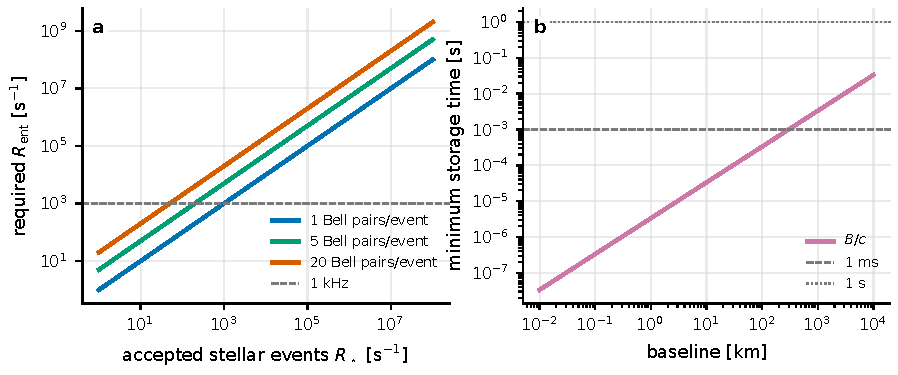
\includegraphics[width=0.94\linewidth]{figures/generated/chapter_17/ch17_entanglement_resources.pdf}
\caption{纠缠率和存储时间给出第一层资源闭合条件。左图把被接受的星光事件率 \(R_\star\) 换成所需纠缠对速率：每个事件消耗的纠缠对越多，需求线抬得越高。右图把基线换成光行时 \(B/c\)：对公里级基线，光行时只是微秒到毫秒，但窄带存储方案常常由测量窗口和纠缠生成时间说了算。}
\label{fig:e24-entanglement-resources}
\end{figure}

第三项是\textbf{保真度}。资源预算里常把链路上几个主要折损因子直接\emph{相乘}，得到一个粗略的有效保真度：

\begin{equation}
  F_{\rm eff}
  \simeq
  F_{\rm Bell}\,
  \eta_{\rm write}\,\eta_{\rm read}\,\eta_{\rm conv}\,
  e^{-T/T_2}\,
  (1-p_{\rm dark})\,
  M_{\rm mode}.
  \label{eq:e24-effective-fidelity}
\end{equation}
\begin{formulaexplain}
\(F_{\rm eff}\) 是粗略的有效资源质量，把纠缠对保真度 \(F_{\rm Bell}\)、写入/读出效率、频率转换效率、存储退相干 \(e^{-T/T_2}\)、暗触发 \((1-p_{\rm dark})\) 与模式匹配 \(M_{\rm mode}\) 全乘在一起。\emph{任何一项偏低，都会乘法式地拉低最终可见度}。
\end{formulaexplain}

逐个点名单位：\(F_{\rm Bell}\)（无量纲，\(\le1\)）是预共享纠缠对的保真度；\(\eta_{\rm write},\eta_{\rm read}\)（无量纲）是写入、读出效率；\(\eta_{\rm conv}\) 是频率转换效率；\(T_2\) 是存储的相干时间（单位 s），\(T\) 是实际存储时长；\(p_{\rm dark}\) 是等效暗触发概率；\(M_{\rm mode}\le1\) 表示频率、时间、偏振、空间四种模式的匹配程度。这不是一条完整的量子信道模型，但它有个好处：\emph{一眼暴露瓶颈}。单看退相干一项，\(T/T_2=1\) 就给 \(e^{-1}\simeq0.37\) 的因子；再假设 \(F_{\rm Bell}=0.8\)、读写各 \(0.7\)、转换 \(0.8\)，暗计数和模式失配还没算，乘起来 \(0.8\times0.7\times0.7\times0.8\simeq0.31\)——最终可见度已经只剩三成上下。这就是为什么这类方案不能只盯着"角分辨率多诱人"，而必须让每一项\emph{同时}闭合。

\begin{figure}[tbp]
\centering
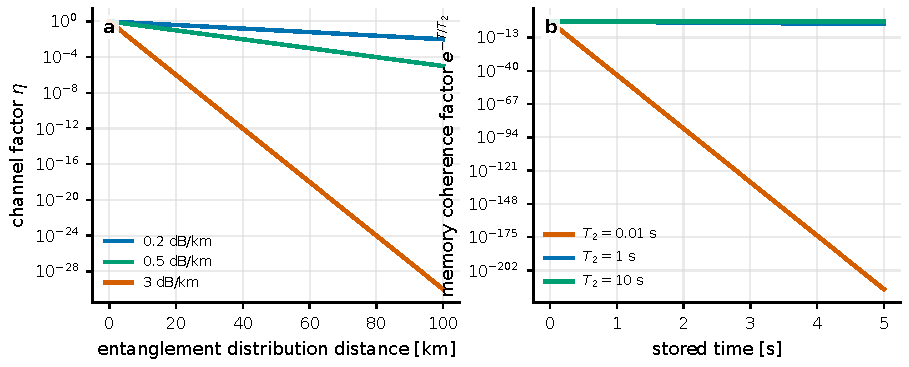
\includegraphics[width=0.94\linewidth]{figures/generated/chapter_17/ch17_fidelity_distance.pdf}
\caption{有效资源质量由链路和存储共同决定。左图给出不同 \(\mathrm{dB\,km^{-1}}\) 损耗下的通道因子随距离的下降；右图给出存储退相干因子 \(e^{-T/T_2}\) 随存储时长的下降。一个长基线方案即使角分辨率再诱人，也要让纠缠对保真度、读写效率、频率转换和存储相干\emph{一起}达标。}
\label{fig:e24-fidelity-distance}
\end{figure}

其中\textbf{频率转换}是天文版本特有的额外难题。许多量子存储材料强耦合的频率并不落在我们想观测的天文波段，而长距离光纤又偏爱电信波段——于是必须做\emph{量子频率转换}：在改变光子频率的同时，保住它的单光子相干、偏振或时间小格编码，还要压住转换过程引入的噪声。尤其要命的是模式匹配：若转换后的谱宽、中心频率、时间波包、偏振和星光对不齐，哪怕只差 \(1\%\)，损失的\emph{也不只是 \(1\%\) 的光子数}——它会直接扣在干涉可见度上，因为可见度衡量的正是两束光"长得有多像" \citep{1990OptL...15.1476K,2010EPJD...58....1S,2016JMOp...63.2005H,2024SPIE13095E..1NR}。

\section{连续变量与辅助单光子：另外两条路各解决什么}
\label{sec:e24-cv-ancilla}

上面的方案都把"左/右路径"当成一个离散的 qubit，再把时间信息塞进存储。还有两类互补的想法，解决的是不同的瓶颈。

第一类是\textbf{连续变量}（continuous variable）路线。这里的"连续变量"指光场的两个正交分量（quadrature），也就是复振幅箭头（第 \ref{chap:e01} 章）的实部和虚部，而不是"左/右"这样非此即彼的离散选择。连续变量的量子隐形传态用一份预共享的\emph{两模压缩真空态}（two-mode squeezed vacuum, TMSV）当资源，靠本地测量把一个模式的正交分量信息转移到远端：

\begin{equation}
  |\psi_{\rm TMSV}\rangle
  =
  \sqrt{1-\lambda^2}\,
  \sum_{n=0}^{\infty}\lambda^n\,|n\rangle_A|n\rangle_B,
  \qquad
  \bar N=2\sinh^2 r .
  \label{eq:e24-tmsv}
\end{equation}
\begin{formulaexplain}
\(|\psi_{\rm TMSV}\rangle\) 是两模压缩真空资源态，\(A,B\) 是相隔很远的两个模式；\(\lambda=\tanh r\)（\(r\) 是压缩参数）控制压缩强度，\(\bar N\) 是总平均光子数。压缩越强，连续变量隐形传态的附加噪声越小，但资源成本越高。
\end{formulaexplain}

这条式子说的是：\(A\) 端和 \(B\) 端的光子数\emph{总是相等}（都取到 \(n\)），而且不同 \(n\) 的振幅按 \(\lambda^n\) 排布——这正是"两模一起被压缩"的量子指纹。理想情形要 \(r\to\infty\)（无穷强压缩）才能无噪声地传送任意连续变量态；现实里 \(r\) 有限，就会掺进一份等效的高斯噪声，通常按 \(e^{-2r}\) 的速度随压缩增强而衰减。Braunstein--Kimble 给出的连续变量隐形传态协议，加上 Gottesman 等的分析，说明这条路能\emph{绕开}离散贝尔测量那个 \(50\%\) 上限；但代价是连续变量的中继更难、远距离的高保真压缩资源也更娇气。最新的最优性分析还提醒：比较不同资源态时，必须把\emph{光子数超选择定则}、局域性和有限的纠缠预算都算进去——压缩度只是账本里的一项，不是全部 \citep{1998PhRvL..80..869B,2012PhRvL.109g0503G,2025PhRvR...7d3278Z}。

第二类是\textbf{辅助单光子}路线，好处是\emph{不依赖长寿命量子存储}。Marchese--Kok 的想法是：让脆弱的星光光子尽早在接收端就地测量掉，改让一个"地面产生、坏了能重做"的辅助单光子去跨基线传输——这样损耗主要落在\emph{可以重来}的地面光子上，而不是不可再生的星光上。对一个小角度的位置估计，相位与角度、以及可达的角度精度满足

\begin{equation}
  \phi=\frac{2\pi B\theta}{\lambda},
  \qquad
  \sigma_\theta
  \ge
  \frac{\lambda}{2\pi B}\,
  \frac{1}{\sqrt{N_{\rm ev}\,\mathcal F_\phi}} .
  \label{eq:e24-angle-fisher}
\end{equation}
\begin{formulaexplain}
左式是角位置 \(\theta\) 与干涉相位 \(\phi\) 的换算；右式是角度误差的下界，\(N_{\rm ev}\) 是有效事件数，\(\mathcal F_\phi\) 是\emph{单个事件}的相位 Fisher 信息（第 \ref{chap:e12} 章）。基线越长、事件越多、单事件信息越高，定位就越精。
\end{formulaexplain}

右式其实就是第 \ref{chap:e12} 章 Fisher 信息 \eqref{eq:e12-fisher-def} 给出的 Cramér--Rao 下界 \eqref{eq:e12-crb} 套在相位估计上的结果：总信息是单事件信息 \(\mathcal F_\phi\) 乘以事件数 \(N_{\rm ev}\)，误差按 \(1/\sqrt{N_{\rm ev}\mathcal F_\phi}\) 下降，前面的 \(\lambda/(2\pi B)\) 是把相位误差换算成角度误差的几何系数——\(B\) 越大，同样的相位误差对应越小的角度误差，这就是长基线的杠杆。Marchese--Kok 在 \(\lambda=628\,\mathrm{nm}\)、光纤衰减长度 \(L_0=10\,\mathrm{km}\) 的模型里，得到十几 \(\mu\mathrm{as}\) 量级的定位标度。Modak--Kok 进一步泼了盆冷水：星光模式占据数 \(\epsilon\ll1\) 和"辅助光子与星光到底有多不可区分"会显著改变收益——若 \(\epsilon\) 从 1 掉到 \(0.01\)，多加辅助光子的好处很快变弱；若模式不可区分度只有 \(96\%\)，三光子方案或许还有赚头，但继续堆更多光子并不一定继续改善 \citep{2023PhRvL.130p0801M,2025PhRvA.111d3701M}。

Padilla、Sajjad、Saif 与 Guha 把问题推到更一般的多模成像极限：先在每个接收站做\emph{本地空间模式排序}（借第 \ref{chap:e12} 章 SPADE 那类技巧），再用预共享纠缠对去模拟一个非局域的合束器乃至更一般的干涉网络。这提醒我们，长基线只是资源的一部分——单孔径内的模式信息、源结构先验、阵列几何、测量基的选择，都会改变最终能榨出的 Fisher 信息。对一对双星的角分离：若只盯着 Rayleigh 标度下的 \(\lambda/B\)，就会错过本地模式排序在\emph{小分离}上的优势；若只追本地超分辨，又拿不到长基线那根相位杠杆。两者要合起来用 \citep{2026PhRvA.113a2608P,2025PhRvR...7d3278Z}。

\section{从实验原型到误差预算}
\label{sec:e24-prototype}

实验原型的价值，不只是证明"能把两个远端节点纠缠起来"，更在于给资源账本里的\emph{每一项都填上可测的数字}。Stas 等在 2026 年的实验，把"非局域相位测量"从线路图搬上了实验台。他们用两个 SiV 金刚石纳米腔节点，配上电子自旋和 \({}^{29}\mathrm{Si}\) 核自旋存储：先生成一对远程纠缠，再让弱信号光在本地与节点相互作用，通过\emph{光子擦除}和非局域的非破坏性预报（heralding）滤掉真空事件。实验里电子贝尔态可达 \(F=0.83(3)\)；纠缠率为 \(13\,\mathrm{Hz}\) 时 \(F\ge0.5\)，降到 \(1.9\,\mathrm{Hz}\) 时 \(F=0.79(3)\)。完整的非局域相位测量中，预报把可见度从"不预报"的 \(0.031(18)\) 提升到 \(0.090(26)\)；再接入 \(1.55\,\mathrm{km}\) 的光纤基线后，核自旋宇称振荡的可见度是 \(0.11(4)\)，而纠缠对保真度仍高于可验证纠缠的阈值，约 \(F=0.63(3)\) \citep{2026Natur.651..326S}。这些数字虽然离天文可用还很远，却第一次把上一节账本里抽象的 \(F_{\rm Bell}\)、\(R_{\rm ent}\)、\(V_{\rm meas}\) 变成了台面上量得出的量。

这类实验的相位误差，由有效试验次数、预报成功率和实测的相位振荡可见度共同决定。用 Fisher 信息写出来：

\begin{equation}
  \mathcal I_\phi
  \simeq
  N_{\rm tr}\,p_{\rm succ}\,V_{\rm meas}^2,
  \qquad
  \mathrm{Var}(\hat\phi)\ge\mathcal I_\phi^{-1} .
  \label{eq:e24-fisher-visibility}
\end{equation}
\begin{formulaexplain}
\(\mathcal I_\phi\) 是总相位 Fisher 信息，\(N_{\rm tr}\) 是试验次数，\(p_{\rm succ}\) 是预报成功概率，\(V_{\rm meas}\) 是实测可见度。可见度以\emph{平方}进入信息量，所以一点点相干损失就会明显放大相位误差；右式是相应的 Cramér--Rao 下界。
\end{formulaexplain}

这里 \(N_{\rm tr}\) 是协议跑了多少次（无量纲），\(p_{\rm succ}\) 是一次试验被接受的概率，\(V_{\rm meas}\) 是相位振荡的可见度。\(V_{\rm meas}^2\) 里的那个平方是关键：可见度掉到 \(1/3\)，信息就掉到 \(1/9\)。而 \(p_{\rm succ}\) 本身又拆成

\begin{equation}
  p_{\rm succ}=\eta_{\rm erasure}\,\eta_{\rm herald}\,P(n_{\rm photon}\ge1),
  \label{eq:e24-psucc}
\end{equation}
\begin{formulaexplain}
\(p_{\rm succ}\) 是一次试验被接受的概率，由光子擦除效率 \(\eta_{\rm erasure}\)、预报探测效率 \(\eta_{\rm herald}\) 和"至少来一个光子"的概率 \(P(n_{\rm photon}\ge1)\) 三者相乘。想提高它，\emph{不能}靠一味加大光强。
\end{formulaexplain}

这条式子藏着一个反直觉的陷阱。你也许会想："成功率 \(p_{\rm succ}\) 越高越好，那就把 \(P(n_{\rm photon}\ge1)\) 拉高——多灌点光子不就行了？"可一旦平均光子数上去，\emph{多光子污染}也跟着上来：一次试验里混进两个甚至更多光子，会破坏干涉、把 \(V_{\rm meas}\) 拉低。而 \(V_{\rm meas}\) 是平方进 \(\mathcal I_\phi\) 的，\(p_{\rm succ}\) 只是一次方——于是 \(p_{\rm succ}\) 涨一点、\(V_{\rm meas}\) 跌一点，总 Fisher 信息 \(\mathcal I_\phi=N_{\rm tr}p_{\rm succ}V_{\rm meas}^2\) 反而\emph{不升反降}。这就是为什么"预报成功率高"不见得是好事。最后把相位误差用式 \eqref{eq:e24-angle-fisher} 换成角度误差：\(B\) 越长，同样的 \(\sigma_\phi\) 对应越小的 \(\sigma_\theta\)，但长基线也会推高纠缠分发的开销、相位锁定的难度和延迟。

\begin{figure}[tbp]
\centering
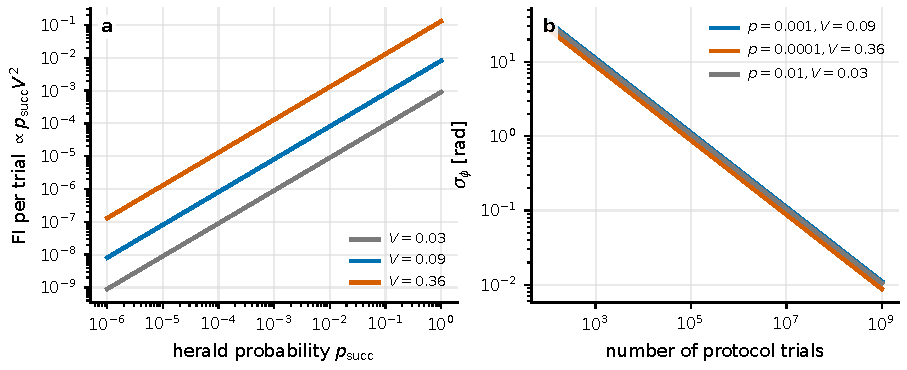
\includegraphics[width=0.94\linewidth]{figures/generated/chapter_17/ch17_fisher_visibility.pdf}
\caption{非局域相位测量的统计收益，同时取决于成功概率和可见度。左图画出单次试验 Fisher 信息的标度 \(p_{\rm succ}V^2\)：可见度降三倍，信息降九倍。右图把试验次数换成相位误差，说明高重复率、低误预报和高纠缠保真度必须\emph{同时}成立，才谈得上有用。}
\label{fig:e24-fisher-visibility}
\end{figure}

Crawford 等的两光子精密天体测量实验，提供了另一级近期台阶：用两个准热光源和时间标记探测器，在桌面模拟装置里看到光子对符合随相位变化的相关行为。这个实验不等于一台完整的量子网络望远镜，但它非常适合当\emph{上天前的排练}——时间标记、偏振匹配、相干时间、HBT 峰拟合、相位稳定、数据筛选，这些环节都和真实的天文弱光观测直接相关 \citep{2023OExpr..3144246C}。

把所有资源摆进同一张图，可以看清我们身处何处：近期实验大致落在 \(R_{\rm ent}\sim1\)–\(10\,\mathrm{Hz}\)、短基线、低有效可见度的角落；而天文可用的"存储辅助窄带"方案，可能需要 \(R_{\rm ent}\sim\mathrm{kHz}\) 到 \(100\,\mathrm{kHz}\)、\(T_{\rm mem}\sim\mathrm{ms}\) 到 \(\mathrm{s}\)、几十个存储 qubit 和很高的模式匹配；宽带成像则更难。四项约束必须\emph{一起}闭合：\(R_{\rm ent}\) 不够会白白浪费星光事件，\(T_{\rm mem}\) 不够会让宇称校验赶不上，\(F_{\rm eff}\) 不够会把可见度洗掉，\(R_\star\) 一旦估错，整套方案可能在第一晚观测之前就已经失去可行性。

\begin{figure}[tbp]
\centering
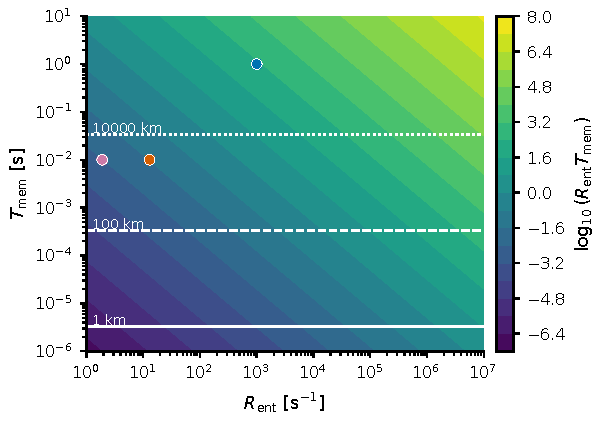
\includegraphics[width=0.94\linewidth]{figures/generated/chapter_17/ch17_network_parameter_space.pdf}
\caption{量子网络望远镜的资源空间，由纠缠率和存储时间共同张开。白线标出 \(1\,\mathrm{km}\)、\(100\,\mathrm{km}\) 和 \(10^4\,\mathrm{km}\) 基线对应的 \(B/c\) 时间；散点给出当前实验的 Hz 级纠缠率与远期 kHz--s 级目标的量级差距。颜色只是资源乘积的标度，完整可行性还要再乘上保真度、模式匹配和天文光子率。}
\label{fig:e24-network-space}
\end{figure}

\section{量子网络和强度干涉怎样互补}
\label{sec:e24-complementarity}

请务必别把量子网络望远镜写成"取代强度干涉"的东西——它是一条\emph{长期互补}的路线。回顾一下两者的分工：第 \ref{chap:e10} 章的强度干涉，靠本地时间标记加离线相关，早就绕开了光学相位传输，几乎不怕大气抖动，代价是主要只拿到 \(|V|^2\)，相位丢了；量子网络路线想\emph{保住}一阶相干的相位，代价则是要支付纠缠、存储、频率转换、预报这一整本资源账。短期内，两者都得和 ELT、VLTI、CHARA、CTAO 以及强度干涉阵列并行发展。

一个务实的分期路线是这样的。\emph{近期}目标是强度干涉和两光子相关：硬件已经接近现成——大面积集光器、SNSPD/SPAD 时间标记、窄带滤光、离线相关，科学目标集中在亮星角直径、双星和发射线区域。\emph{中期}加入本地空间模式排序、两光子天体测量和 GJC 型短基线的上天演示，目标是证明星光模式能和实验室纠缠资源\emph{稳定地干涉}。\emph{远期}才是存储辅助的非局域一阶相干测量，它要求量子存储、频率转换、纠缠分发、纠缠保真度和天文仪器同步一起成熟 \citep{1956Natur.178.1046H,2023OExpr..3144246C,2024SPIE13095E..1NR,2026Natur.651..326S}。

\Needspace{11\baselineskip}
观测规划可以从一个简洁的闭合条件出发：

\begin{equation}
  N_{\rm useful}
  =
  R_\star\,T_{\rm obs}\,
  p_{\rm ready}\,p_{\rm succ}\,V_{\rm meas}^2
  \gtrsim
  N_{\rm req}(\sigma_\theta,\bm{B},\lambda) .
  \label{eq:e24-useful-events}
\end{equation}
\begin{formulaexplain}
\(N_{\rm useful}\) 是真正带相位信息的有效事件数，等于星光事件率、观测时间、资源就绪概率、成功率和可见度平方的乘积；\(N_{\rm req}\) 是达到目标角精度 \(\sigma_\theta\) 所需的事件数。只有 \(N_{\rm useful}\ge N_{\rm req}\)，方案才有观测意义。
\end{formulaexplain}

逐项点名：\(T_{\rm obs}\) 是总观测时间（s），\(N_{\rm req}\) 由目标角精度、阵列几何和模型参数维数决定。这条式子把天文学和量子工程放进了\emph{同一本账}：又亮、又窄带、到达时间或周期已知的信号，会降低资源压力；又暗、又宽带的连续源，则会把所有困难一起放大。值得强调的是，同一本账也适用于更一般的观测设计，只是可观测量从"非局域相位"换成 \(|V|^2\)、\(g^{(2)}\)、偏振角或时间延迟而已。

所以，量子网络望远镜眼下最有价值的产物，\emph{不是}某台已经造好的仪器，而正是这张可以一项项核对的可行性账本。下一章我们回到观测设计的主线：把科学目标落到事件率、通道、基线、背景和协方差上，然后才谈得上在强度干涉、偏振事件表、瞬变触发与未来的非局域相位测量之间做取舍。

\section*{本章要点}
\addcontentsline{toc}{section}{本章要点}

\begin{itemize}
\item \textbf{瓶颈的来源。} 长基线振幅干涉要把稀少的星光单光子送到同一个合束器，可链路损耗随距离\emph{指数}上升（式 \eqref{eq:e24-link-loss}），而基线越长分辨率越高（式 \eqref{eq:e24-resolution-scale}）——诱惑和困难来自同一个量纲。
\item \textbf{换掉要搬运的东西。} Gottesman--Jennewein--Croke 用一个已知、可验证、可重来的预共享纠缠光子 \eqref{eq:e24-lab-entangled-photon} 替代长途搬运星光；扫描本地相位 \(\delta\) 就能从符合点击率 \eqref{eq:e24-gjc-probability} 读出复可见度 \(V\)。线性光学的贝尔测量带来约 \(50\%\) 的事件损失。
\item \textbf{弱光的稀疏性是朋友。} 每个窗口平均只有 \(\epsilon\ll1\) 个星光光子，于是二进制时间小格编码把资源从 \(M\sim1/\epsilon\) 个纠缠对压到约 \(\log_2 M\) 个存储 qubit（式 \eqref{eq:e24-binary-timebin}）——量子中继与量子存储负责把概率性成功事件对齐。
\item \textbf{四项要一起闭合。} 纠缠供应率 \eqref{eq:e24-entanglement-rate}、存储时间 \eqref{eq:e24-memory-time}、有效保真度 \eqref{eq:e24-effective-fidelity} 和有效星光事件率必须同时达标；保真度是各因子\emph{相乘}，任一项偏低都会乘法式洗掉可见度。频率转换的模式失配尤其致命。
\item \textbf{还有两条互补路。} 连续变量隐形传态用两模压缩真空 \eqref{eq:e24-tmsv} 绕开 \(50\%\) 上限但资源更娇气；辅助单光子路线 \eqref{eq:e24-angle-fisher} 让可重来的地面光子去承担链路风险，收益却对 \(\epsilon\) 和模式不可区分度敏感。
\item \textbf{可见度以平方进信息。} 实验的相位 Fisher 信息标度为 \(p_{\rm succ}V_{\rm meas}^2\)（式 \eqref{eq:e24-fisher-visibility}）；一味加大光强会引入多光子污染、压低 \(V_{\rm meas}\)，反而降低总信息——量子网络与强度干涉应当分期并行、长期互补（式 \eqref{eq:e24-useful-events}）。
\end{itemize}

\medskip
\noindent\textbf{想一想。}
\begin{enumerate}
\item 若把观测带宽 \(\Delta\nu\) 从 \(10\,\mathrm{GHz}\) 收窄到 \(1\,\mathrm{MHz}\)，直接 GJC 路线每秒要准备的纠缠光子数、以及二进制时间小格方案所需的存储 qubit 数，各会怎样变化？为什么"窄带"反而对存储辅助方案有利？
\item 在有效保真度 \eqref{eq:e24-effective-fidelity} 里，若你只能改善一个环节，你会先攻哪一项？把 \(T/T_2\)、读写效率、频率转换效率各改善 \(10\%\)，分别对 \(F_{\rm eff}\) 带来多大提升？
\item 为什么"提高预报成功率 \(p_{\rm succ}\)"不一定提高总 Fisher 信息 \(\mathcal I_\phi\)？用式 \eqref{eq:e24-fisher-visibility} 和 \eqref{eq:e24-psucc} 说明多光子污染在什么条件下会让收益反转。
\end{enumerate}

\chapter{第一代量子天文学科学案例}
\label{chap:e25}

\begin{chapteropening}
前面几个部分，我们像攒装备一样把工具一件件配齐了：复振幅与相位（第 \ref{chap:e01} 章）、带宽与相干时间（第 \ref{chap:e02} 章）、泊松与散粒噪声（第 \ref{chap:e03} 章）、二阶相干 \(g^{(2)}\) 与 Siegert 关系（第 \ref{chap:e08} 章）、强度干涉与 van Cittert--Zernike 定理（第 \ref{chap:e10} 章）、从可见度到成像（第 \ref{chap:e11} 章）、量子估计与 SPADE（第 \ref{chap:e12} 章）、事件表与时钟（第 \ref{chap:e13} 章）、误差预算（第 \ref{chap:e15} 章），一直到把恒星当成量子光源（第 \ref{chap:e17} 章）、把瞬变缝成多信使事件（第 \ref{chap:e20} 章）。装备齐了，就该下场打仗。本章要回答一个非常实际的问题：\textbf{在今天这套仪器条件下，第一代量子天文学到底能做哪些"现在就能做"的真科学？}我们会沿着一条清单走下去——亮星角直径、快速自转的扁球、密近双星、Be 星盘与 Wolf--Rayet 风、新星与 Type Ia 的膨胀、Crab 的光子统计、自然激光候选——每到一站都问同样三件事：\textbf{要测什么可观测量？需要什么样的阵列、曝光和精度？它能回答哪个天体物理问题？}这不是画大饼，而是把前面每一章的公式，落到明晚就能对准的目标上。
\end{chapteropening}

\section{给案例排序：亮度、角尺度、外部先验这三把尺子}
\label{sec:e25-triage}

打仗不能一拥而上。第一代项目最怕的不是"题目不够漂亮"，而是"漂亮题目却做不出结果"。所以在挑目标之前，先要建立一套冷静的排序法，让科学价值、技术可行性、失败后仍有产出这三件事同时进入判断。

\textbf{第一把尺子是亮度。}强度干涉（intensity interferometry）的信号是符合计数（coincidence），它的统计精度最终由攒到的\textbf{光子对数}决定（第 \ref{chap:e15} 章）。光子率越高，同样时间里攒的对数越多，误差按对数平方根往下掉。对当前这一代仪器，一个粗略的分区是：视星等 \(m_V\lesssim5\) 的热星是"验证区"，信号强、能反复复现；\(m_V\simeq6\text{--}7\) 是"有挑战但能规划"的区域；\(m_V\gtrsim9\) 通常就得靠更大阵列、多谱通道、更长积分或更低系统噪声才够得着。LeBohec 与 Holder 的估算给了一个可以记住的锚点：一对 \(100\,\mathrm{m^2}\)、电子带宽到 GHz 量级的望远镜，5 小时内可以对 \(m_V\simeq6.7\) 的源做到几倍标准差的相关检出 \citep{2006ApJ...649..399L,2013APh....43..331D}。

\textbf{第二把尺子是角尺度。}亮度决定"有没有光子"，角尺度决定"这些光子能不能变成参数"。第 \ref{chap:e11} 章讲过，一台基线为 \(B\)、波长为 \(\lambda\) 的干涉仪，能分辨的角尺度标度是 \(\lambda/B\)。若目标角尺度 \(\theta\gg\lambda/B\)，那么在长基线上平方可见度 \(|V|^2\) 已经掉到接近零，只有短基线还剩信号；若 \(\theta\ll\lambda/B\)，则所有基线都看到一个"未解析的点"，可见度对直径的导数几乎为零，测了也约束不动参数。两头都不好，最舒服的是让主要结构正好落在你手上的基线区间里——对现有 IACT 阵列是 \(50\text{--}300\,\mathrm{m}\)，对未来 CTA 型阵列是 \(0.5\text{--}2\,\mathrm{km}\)。

\textbf{第三把尺子是外部先验。}同样几个 \(|V|^2\) 数据点，如果你事先知道距离、光谱、轨道、径向速度或一个理论大气模型，它们就能被"翻译"成真正的物理参数；如果什么先验都没有，几个孤零零的可见度点往往互相退化，谁也钉不住谁。所以有成熟先验的目标，天然排在前面 \citep{2003RPPh...66..789M,2012MNRAS.419..172N}。

把这三把尺子写成一个可以打分的排序式，就得到一个实用的分诊（triage）工具：
\begin{equation}
  \mathcal P
  =
  \frac{
  W_{\rm sci}\,
  R_{\rm tech}\,
  R_{\rm prior}
  }{
  1+R_{\rm sys}+R_{\rm trigger}
  } .
  \label{eq:e25-priority-score}
\end{equation}
\begin{formulaexplain}
\(\mathcal P\) 是项目排序分数。分子上，科学回报 \(W_{\rm sci}\)、技术成熟度 \(R_{\rm tech}\)、外部先验 \(R_{\rm prior}\) 越高分越高；分母上，系统误差风险 \(R_{\rm sys}\)、触发/调度风险 \(R_{\rm trigger}\) 越高分越低。它专门用来防止"只凭题目好听"就上马。
\end{formulaexplain}
逐项落地：\(W_{\rm sci}\) 是科学回报（这个结果有多重要），\(R_{\rm tech}\) 是技术成熟度（现有仪器能不能稳定做出来），\(R_{\rm prior}\) 是外部先验与模型可解释性，\(R_{\rm sys}\) 是系统误差风险（零基线相关、时间同步、背景扣除有多容易翻车），\(R_{\rm trigger}\) 是触发与调度风险（要不要抢时间窗、能不能随时开机）。这些量都无量纲，实际使用时只需粗分几档（高/中/低），目的不是算出一个精确小数，而是\textbf{不让单一维度支配选择}。举个对照：Type Ia 的几何距离 \(W_{\rm sci}\) 极高，可它的 \(R_{\rm trigger}\) 和 \(R_{\rm sys}\) 也高，分母被顶起来，第一代不宜强上；亮星角直径的 \(W_{\rm sci}\) 只是中等，却有很高的 \(R_{\rm tech}\) 和很低的系统风险，分数反而稳，特别适合当第一批"验收指标" \citep{2024ApJ...966...28A,2024MNRAS.529.4387A,2025PhRvD.111h3047K}。

\begin{figure}[tbp]
\centering
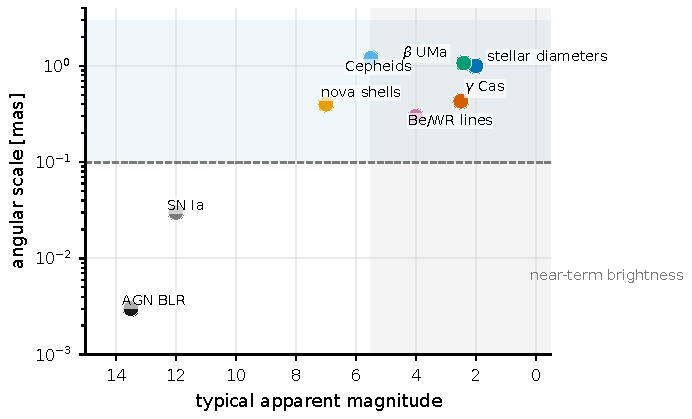
\includegraphics[width=0.88\linewidth]{figures/generated/chapter_19/ch19_science_case_feasibility.pdf}
\caption{第一代候选目标在"亮度--角尺度"平面上的位置。亮星角直径、\(\beta\) UMa、\(\gamma\) Cas 以及 Be/WR 谱线区同时满足"够亮"和"能被百米级基线解析"，落在最舒服的区域；Type Ia、AGN 宽线区和暗物质小尺度透镜科学价值很高，却被亮度、事件率或角尺度推向长期项目。这张图就是式 \eqref{eq:e25-priority-score} 里三把尺子的可视化。}
\label{fig:e25-case-plane}
\end{figure}

有了这套排序，本章后面的顺序其实已经隐含其中：先做落在图 \ref{fig:e25-case-plane} 右上"舒服区"的目标，再一步步往科学价值更高、但风险也更大的方向推进。

\section{恒星角直径与有效温度：第一代最成熟的产品}
\label{sec:e25-diameter}

为什么第一件事是量恒星的\textbf{角直径}（angular diameter）？因为它同时满足前面三把尺子，而且产出直接、可复现、能反复当验收标准。观测量非常干净：在一系列基线 \(B\) 和波长 \(\lambda\) 上测平方可见度 \(|V|^2(B,\lambda)\)，模型从最简单的\textbf{均匀圆盘}（uniform disk）开始，再用\textbf{边缘昏暗}（limb darkening，恒星盘边缘比中心暗）廓线或完整大气模型去修正。

角直径最漂亮的用处，是它能直接钉住恒星的\textbf{有效温度}（effective temperature）。这里的逻辑链一步都不能跳，我们把它铺开。一颗半径 \(R\)、有效温度 \(T_{\rm eff}\) 的恒星，其光度由 Stefan--Boltzmann 定律给出 \(L=4\pi R^2\sigma_{\rm SB}T_{\rm eff}^4\)。这些光子跑到距离 \(D\) 的地球，摊在一个半径为 \(D\) 的球面上，于是我们收到的\textbf{总辐射流量}（bolometric flux）是
\[
  F_{\rm bol}=\frac{L}{4\pi D^2}
  =\frac{R^2}{D^2}\,\sigma_{\rm SB}T_{\rm eff}^4
  =\left(\frac{R}{D}\right)^2\sigma_{\rm SB}T_{\rm eff}^4 .
\]
注意 \(R/D\) 正是恒星的\textbf{角半径}，而角直径 \(\theta_{\rm LD}=2R/D\)，所以 \(R/D=\theta_{\rm LD}/2\)，\((R/D)^2=\theta_{\rm LD}^2/4\)。代回去就得到本节的核心式：
\begin{equation}
  F_{\rm bol}
  =
  \frac{\theta_{\rm LD}^2}{4}
  \sigma_{\rm SB}T_{\rm eff}^4,
  \qquad
  T_{\rm eff}
  =
  \left(
  \frac{4F_{\rm bol}}
  {\sigma_{\rm SB}\theta_{\rm LD}^2}
  \right)^{1/4}.
  \label{eq:e25-teff}
\end{equation}
\begin{formulaexplain}
\(F_{\rm bol}\) 是地球处收到的总辐射流量，\(\theta_{\rm LD}\) 是边缘昏暗角直径，\(\sigma_{\rm SB}\) 是 Stefan--Boltzmann 常数，\(T_{\rm eff}\) 是有效温度。一句话：角直径一旦测准，就能把"流量"直接换算成恒星的"温度尺"。
\end{formulaexplain}
逐个交代单位与量纲：\(F_{\rm bol}\) 单位 \(\mathrm{erg\,s^{-1}\,cm^{-2}}\)，从多波段测光积分得到；\(\theta_{\rm LD}\) 单位 rad（毫角秒 mas 是常用的实用单位，\(1\,\mathrm{mas}=4.85\times10^{-9}\,\mathrm{rad}\)）；\(\sigma_{\rm SB}=5.67\times10^{-5}\,\mathrm{erg\,s^{-1}\,cm^{-2}\,K^{-4}}\)；\(T_{\rm eff}\) 单位 K。这条式子妙在它\textbf{不依赖距离}：\(F_{\rm bol}\) 和 \(\theta_{\rm LD}\) 都是直接可观测的，中间那个 \(D\) 在推导里已经消掉了。

角直径的误差怎样传到温度上？把 \(T_{\rm eff}\) 对 \(\theta_{\rm LD}\) 取对数微分。因为 \(T_{\rm eff}\propto\theta_{\rm LD}^{-1/2}\)（把 \(F_{\rm bol}\) 视为独立测量），有
\[
  \ln T_{\rm eff}=\text{常数}-\tfrac12\ln\theta_{\rm LD}
  \;\Longrightarrow\;
  \frac{\delta T_{\rm eff}}{T_{\rm eff}}=-\frac12\frac{\delta\theta_{\rm LD}}{\theta_{\rm LD}} .
\]
所以角直径 \(4\%\) 的误差，只由这一路传播到温度，就是 \(2\%\)。这个"减半"的关系解释了为什么亮星角直径值得反复测：它不是一次性的仪器炫技，而是会流进 \(T_{\rm eff}\)、恒星半径、年龄、自转模型和标准星尺度的\textbf{基石数据} \citep{1967MNRAS.137..393H,1977MNRAS.180..177B,2003RPPh...66..789M}。

这条路线已经从历史走进了现代。上世纪 Narrabri 强度干涉仪用 Hanbury Brown 和 Twiss 的方法量过一批亮星直径 \citep{1956Natur.178.1046H,1974MNRAS.167..121H}；今天 VERITAS 的强度干涉系统（VERITAS-SII）把它推进到亚毫角秒精度，对 \(\beta\) CMa 和 \(\epsilon\) Ori 给出直径，且用远少于当年的观测时间就做到优于 \(5\%\)；后续对 \(\beta\) UMa 在 416 nm 得到边缘昏暗角直径 \(\theta_{\rm LD}=1.07\pm0.04_{\rm stat}\pm0.05_{\rm sys}\,\mathrm{mas}\)，并与 CHARA 近红外、Keck 中红外结果互相校验。MAGIC 的升级系统（MAGIC-SII）更是一口气报告了 22 个恒星直径，其中 13 个此前没有可比测量——强度干涉已经从"单次演示"变成"成批出数据" \citep{2020NatAs...4.1164A,2024ApJ...966...28A,2024MNRAS.529.4387A}。这里要提醒的一点是：这些结果用的是\textbf{二阶}相干（第 \ref{chap:e08}、\ref{chap:e10} 章），它对大气宁静度和光路相位不敏感，这正是它在窄带、超长基线上仍能工作的原因。

\textbf{要什么、答什么？}这一案例需要的阵列很朴素：几对现成 IACT 望远镜、百米级基线、窄带滤光、GHz 级电子带宽、几小时到几夜的积分；精度目标是把直径做到 \(3\text{--}5\%\)、多夜可复现。它回答的是恒星物理里最基础的问题——\textbf{这颗星到底多大、多热}，进而校准整条恒星参数与距离尺度。

\section{快速自转：从"多大"升级到"什么形状"}
\label{sec:e25-rotation}

量到直径只是第一步。很多热星转得极快，快到离心力把赤道甩得鼓出来，光球变成一个扁椭球；而且按 von Zeipel 定理，鼓出去的赤道引力小、温度低、更暗，两极则又亮又热——这就是\textbf{重力昏暗}（gravity darkening）。要看见这种结构，均匀圆盘模型就不够了：它只有一个参数 \(\theta\)，而一个扁椭球至少需要三个参数——短轴角直径 \(\theta_{\rm min}\)、\textbf{轴比}（axial ratio）\(r=\theta_{\rm maj}/\theta_{\rm min}\)、以及位置角 \(\varphi_\star\)。

怎样把这个扁球写成可拟合的可见度曲线？先回忆第 \ref{chap:e11} 章的已知结果：一个角直径为 \(\theta\) 的均匀圆盘，其一阶可见度模长是 Airy 形式 \(|V|=|2J_1(x)/x|\)，其中 \(x=\pi B\theta/\lambda\) 是无量纲空间频率，\(J_1\) 是一阶 Bessel 函数（圆孔径衍射的标准结果，第一个零点在辐角 \(3.83\)）。椭球的诀窍在于：沿不同方向投影，看到的"有效直径"不同——沿短轴看是 \(\theta_{\rm min}\)，沿长轴看是 \(r\theta_{\rm min}\)。把这个方向依赖装进 \(x\)，就得到
\begin{equation}
  x_{\rm ell}
  =
  \frac{\pi B_p\theta_{\rm min}}{\lambda}
  \left[
  \cos^2\psi
  +
  r^2\sin^2\psi
  \right]^{1/2},
  \qquad
  |V_{\rm ell}|^2
  =
  \left[\frac{2J_1(x_{\rm ell})}{x_{\rm ell}}\right]^2 .
  \label{eq:e25-elliptical-visibility}
\end{equation}
\begin{formulaexplain}
\(x_{\rm ell}\) 是扁椭球在当前投影基线上的无量纲空间频率，\(B_p\) 是投影基线长度，\(\psi\) 是投影基线相对短轴的方向角，\(r\) 是轴比。方括号里的因子把"看的方向"折进了有效直径：沿短轴（\(\psi=0\)）它退回 \(\theta_{\rm min}\)，沿长轴（\(\psi=90^\circ\)）它变成 \(r\theta_{\rm min}\)。
\end{formulaexplain}
把方括号验一眼就懂它的几何：当 \(\psi=0\)（基线正对短轴），\(\cos^2\psi=1,\sin^2\psi=0\)，\(x_{\rm ell}=\pi B_p\theta_{\rm min}/\lambda\)，看到的是短轴；当 \(\psi=90^\circ\)，\(x_{\rm ell}=\pi B_p(r\theta_{\rm min})/\lambda\)，看到的是长轴。参数落地：热星轴比典型在 \(r\simeq1.1\text{--}1.5\)，短轴角直径常小于 \(1\,\mathrm{mas}\)。这里有个关键的\textbf{观测设计}教训：要同时钉住 \(r\) 和 \(\varphi_\star\)，你必须在\textbf{多个位置角}上都拿到 \(|V|^2\)——单方向的基线覆盖会让 \(r\) 和 \(\varphi_\star\) 严重退化，因为一条曲线可以由"更扁但转个角度"和"没那么扁"共同拟合。这正是第 \ref{chap:e11} 章 uv 覆盖那套语言在具体目标上的兑现。

现实里这已经做出来了。VERITAS 对经典快速自转星 \(\gamma\) Cas 的观测给出短轴角直径约 \(0.43\pm0.02_{\rm stat}\pm0.02_{\rm sys}\,\mathrm{mas}\)、轴比约 \(1.28\pm0.04\pm0.02\)、自转轴位置角约 \(116^\circ\)，并用 Roche--von Zeipel 模型推断它已接近\textbf{临界自转}（breakup rotation，赤道离心力接近平衡引力）\citep{2025ApJ...995..191A}。这意味着第一代强度干涉已经能从"这颗星多大"推进到"这颗星是什么形状、两极和赤道差多少温度"。

\textbf{要什么、答什么？}这一案例需要在同一目标上覆盖\textbf{两个以上明显不同的位置角}，其余要求与角直径相同；精度目标是能在统计上区分圆盘模型与椭圆模型。它回答的是恒星结构与演化里的一个深问题——\textbf{自转如何改变恒星的形状、温度分布乃至寿命}。

\section{双星、Be 星盘与 Wolf--Rayet 风：用基线把它们分开}
\label{sec:e25-binary}

强度干涉不止能测"一个源有多大"，也能把"其实是两个源"识破。\textbf{密近双星}（close binary）的好处是它的信号有极高的辨识度。设两个都未被解析的点源，角分离向量为 \(\bm s\)，\textbf{流量比}（flux ratio）\(f=F_2/F_1\)。它们的合成相干函数是各自复振幅按流量加权的叠加，归一化后为 \((1+f\,e^{-2\pi i\,\bm u\cdot\bm s})/(1+f)\)，其中 \(\bm u=\bm B_\perp/\lambda\) 是空间频率。平方可见度就是它的模平方，我们把这一步展开，一格都不跳：
\[
  |V_{\rm binary}|^2
  =\frac{|1+f e^{-i\phi}|^2}{(1+f)^2},
  \qquad \phi\equiv 2\pi\,\bm u\cdot\bm s .
\]
利用 \(|1+f e^{-i\phi}|^2=(1+f\cos\phi)^2+(f\sin\phi)^2=1+2f\cos\phi+f^2\cos^2\phi+f^2\sin^2\phi=1+f^2+2f\cos\phi\)（这里只用了 \(\cos^2+\sin^2=1\)），得到
\begin{equation}
  |V_{\rm binary}|^2
  =
  \frac{1+f^2+2f\cos(2\pi\,\bm u\cdot\bm s)}
  {(1+f)^2}.
  \label{eq:e25-binary-visibility}
\end{equation}
\begin{formulaexplain}
\(\bm u=\bm B_\perp/\lambda\) 是空间频率，\(\bm s\) 是双星角分离向量，\(f\) 是流量比。指数里的相位随基线变化，使 \(|V|^2\) 沿基线上下\textbf{振荡}——正是这条振荡曲线让强度干涉能约束双星的分离与方向。
\end{formulaexplain}
读这条式子的关键是那个余弦项的\textbf{振幅} \(2f/(1+f)^2\)。当 \(f=1\)（等亮双星），\(|V|^2\) 会从 \(1\)（当 \(\cos=+1\)）一路振荡到 \(0\)（当 \(\cos=-1\)），信号又深又好认；当 \(f=0.1\)（暗伴星只有主星十分之一亮），余弦项的半振幅只剩 \(2(0.1)/(1.1)^2\simeq0.17\)，而 \(|V|^2\) 是围绕均值 \((1+f^2)/(1+f)^2=1.01/1.21\simeq0.83\) 上下摆动这个半振幅，也就是从谷值 \((1-f)^2/(1+f)^2=(0.9/1.1)^2\simeq0.67\) 起伏到峰值 \(1.0\)，调制深度只有约 \(0.33\)，对信噪比和校准的要求陡然提高。振荡的\textbf{周期}则由分离 \(\bm s\) 定：分离越大，\(|V|^2\) 随基线振荡越快。所以双星项目最适合那些\textbf{已有光谱轨道或食双星先验}的系统——每夜只需拿到少数几个基线点，就能被已知轨道模型串起来；即便某夜失败，也能给出分离或亮度比的上限，不至于颗粒无收 \citep{1974MNRAS.167..121H,2012MNRAS.419..172N,2014MNRAS.437..798M,2022MNRAS.512.1722K}。

\begin{figure}[tbp]
\centering
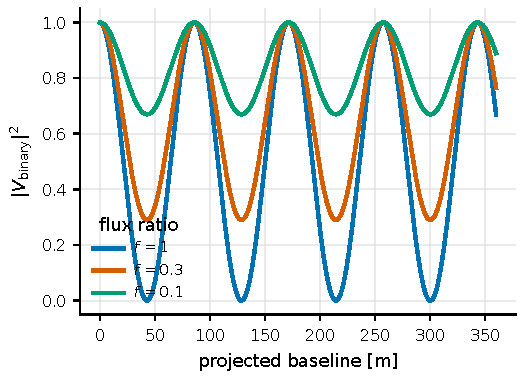
\includegraphics[width=0.82\linewidth]{figures/generated/chapter_19/ch19_binary_visibility.pdf}
\caption{一对 \(1\,\mathrm{mas}\) 双星在 416 nm 下的平方可见度振荡。等亮双星（\(f=1\)）给出从 1 到 0 的深振荡；流量比降到 \(0.3\)、\(0.1\) 后，按式 \eqref{eq:e25-binary-visibility} 的振幅 \(2f/(1+f)^2\) 迅速变浅。双星项目因此格外依赖多位置角的基线覆盖和已知轨道先验，否则亮度比、分离和位置角会互相退化。}
\label{fig:e25-binary-visibility}
\end{figure}

再往前一步，是把"空间分辨"和"谱线选择"结合起来，去解剖\textbf{Be 星盘}（Be decretion disk，快速自转 B 型星抛出的赤道气盘）和\textbf{Wolf--Rayet 风}（大质量恒星的高速星风）。这些源的连续谱主要来自光球，而 \(\mathrm{H}\alpha\)、He、Fe 等发射线却来自更大、更扩展的盘或风碰撞区。麻烦在于，一个滤光片里往往\textbf{谱线和连续谱混在一起}，测到的可见度是两者按通量加权的平均：
\begin{equation}
  V_{\rm obs}
  =
  \frac{
  F_{\rm c}V_{\rm c}
  +
  F_{\rm line}V_{\rm line}
  }{
  F_{\rm c}+F_{\rm line}
  } .
  \label{eq:e25-line-continuum}
\end{equation}
\begin{formulaexplain}
\(V_{\rm c},V_{\rm line}\) 分别是连续谱区与谱线区的可见度，\(F_{\rm c},F_{\rm line}\) 是对应通量。你测到的 \(V_{\rm obs}\) 是二者的通量加权平均，所以谱线几何必须先从连续谱里"减"出来，才能单独解释。
\end{formulaexplain}
其中 \(F_{\rm line}/F_{\rm c}\) 可从同时光谱或"窄带减连续谱"的双滤光片估计。物理判读很直观：如果谱线区比光球\textbf{大}（如展开的盘），那么长基线上的 \(V_{\rm line}\) 会比连续谱掉得更快，混合后的 \(V_{\rm obs}\) 在长基线端被谱线拖低；反过来，如果谱线来自一个很小的高亮斑，长基线上它反而保留信号。历史上 Narrabri 对 Wolf--Rayet 双星 \(\gamma^2\) Velorum 就已经展示了发射线区和连续谱区可以有\textbf{不同的角尺度} \citep{1970MNRAS.148..103H,2010SPIE.7734E..0AD,2012NewAR..56..143D,2025ApJ...995..191A}。现代多基线阵列可以把这一思想推广到 Be 星盘的几何、快速自转热星的谱线轮廓，以及相互作用双星的风碰撞区。

\textbf{要什么、答什么？}这一案例需要窄带滤光或同时光谱来分离谱线与连续谱、可验证的连续谱扣除、以及足够的谱线通量；它回答的是\textbf{恒星如何抛出物质、盘和风是什么几何形状}这类难以用别的手段直接成像的问题。

\section{膨胀的瞬变：新星现在能做，Type Ia 是长期目标}
\label{sec:e25-transient}

现在把镜头转向会"长大"的源。新星、超新星这类爆发抛出一团膨胀外壳，它的几何账本极其简单：若外壳以速度 \(v_{\rm exp}\) 近似自由膨胀，那么爆发后时间 \(t-t_0\) 时，它张开的角直径是"走过的线半径的两倍除以距离"：
\begin{equation}
  \theta(t)
  \simeq
  \frac{2v_{\rm exp}(t-t_0)}{D},
  \qquad
  D
  \simeq
  \frac{2v_{\rm exp}(t-t_0)}{\theta}.
  \label{eq:e25-expansion}
\end{equation}
\begin{formulaexplain}
\(\theta(t)\) 是膨胀外壳的角直径，\(v_{\rm exp}\) 是膨胀速度，\(t_0\) 是爆发时刻，\(D\) 是距离。左式预言"外壳有多大"，右式反解出"离我们多远"——这就是不依赖标准烛光的\textbf{膨胀视差}（expansion parallax）。
\end{formulaexplain}
逐项交代：\(v_{\rm exp}\) 来自谱线的多普勒速度（第 \ref{chap:e20} 章讲过怎样从波长移动读速度），单位 \(\mathrm{cm\,s^{-1}}\)；\(t-t_0\) 是爆发后时间，单位 s；\(D\) 是距离，单位 cm。它的物理前提是一句大白话：\(v_{\rm exp}\) 和 \(\theta\) 必须对应\textbf{同一层物质}，否则右式的距离会系统性偏差（第 \ref{chap:e20} 章详细分析过这个陷阱）。

把两组真实数字代进去，第一代能做什么、不能做什么立刻见分晓。\textbf{银河系新星}：取 \(D=2\,\mathrm{kpc}=6.17\times10^{21}\,\mathrm{cm}\)、\(v_{\rm exp}=10^8\,\mathrm{cm\,s^{-1}}\)、\(t-t_0=10\,\mathrm{d}=8.64\times10^5\,\mathrm{s}\)。线半径 \(v_{\rm exp}(t-t_0)=8.64\times10^{13}\,\mathrm{cm}\)，角直径 \(\theta=\dfrac{2\times8.64\times10^{13}}{6.17\times10^{21}}=2.80\times10^{-8}\,\mathrm{rad}\)。用 \(1\,\mathrm{rad}=2.063\times10^8\,\mathrm{mas}\) 换算，\(\theta\approx5.8\,\mathrm{mas}\)——十天后就到了几毫角秒，用百米以下基线即可解析。\textbf{Type Ia 超新星}：取 \(D=10\,\mathrm{Mpc}=3.09\times10^{25}\,\mathrm{cm}\)、\(v_{\rm exp}=10^9\,\mathrm{cm\,s^{-1}}\)、\(t-t_0=20\,\mathrm{d}=1.73\times10^6\,\mathrm{s}\)。线半径 \(1.73\times10^{15}\,\mathrm{cm}\)，\(\theta=\dfrac{2\times1.73\times10^{15}}{3.09\times10^{25}}=1.12\times10^{-10}\,\mathrm{rad}\approx0.023\,\mathrm{mas}\)——即便速度快十倍，二十天后也只有几十微角秒，需要\textbf{数公里}级光学基线才能碰到。

\begin{figure}[tbp]
\centering
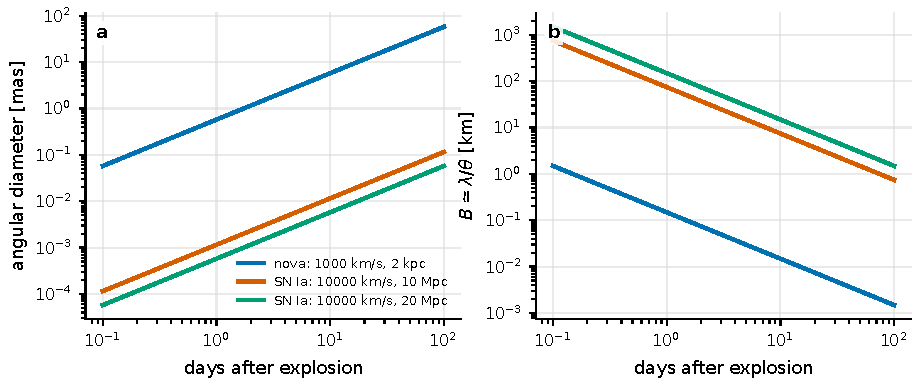
\includegraphics[width=0.94\linewidth]{figures/generated/chapter_19/ch19_transient_expansion.pdf}
\caption{膨胀瞬变的角直径与所需基线。银河系新星在几天到几十天内进入毫角秒量级，适合第一代拿来做"触发--调度--成像"的整套演练；\(10\text{--}20\,\mathrm{Mpc}\) 的 Type Ia 即使在峰值附近也只有几十微角秒，需要公里级基线和 \(m\lesssim12\) 的近邻事件。曲线正是式 \eqref{eq:e25-expansion} 在不同 \(v_{\rm exp}\)、\(D\) 下的走向。}
\label{fig:e25-transient-expansion}
\end{figure}

所以第一代的分工很清楚：\textbf{银河系新星}是现实目标，它角尺度够大、又足够亮，最适合用来把触发（trigger）、滤光、背景扣除、模型拟合的整条流水线跑通，主要困难来自亮度快速演化、外壳非球对称和尘埃遮挡。\textbf{Type Ia 几何距离}则是高回报的长期目标：Kim 等的可行性研究把 \(m\lesssim12\)（对应 \(z\sim0.004\) 的局部体积，全天约每年一个）作为可预见下一代的亮度范围，并用辐射转移模型算出不同波长的表面亮度与 \(|V|^2\)，指出\textbf{光谱分辨}可以提供多波长层析，让测量不再局限于一个均匀圆盘半径 \citep{2025PhRvD.111h3047K,1997A&A...320..799F,2004A&A...415..531S}。换句话说，Type Ia 距离标尺应当排进二代或专用阵列的目标，而不是第一代的验收项。

\textbf{要什么、答什么？}新星案例需要\textbf{快速触发}（几小时内响应）加上同时的谱线速度，把 \(\theta(t)\) 和 \(v_{\rm exp}\) 配对；它回答的是"这次爆发离我们多远、外壳是不是球对称"，并为将来用膨胀视差独立校准宇宙距离阶梯做技术铺垫。

\section{Crab 与自然激光：用光子统计检验"非热"}
\label{sec:e25-statistics}

前面几节都在用\textbf{可见度}（二阶相干的空间信息）。本节换一副眼镜，用\textbf{时间统计}——这正是事件表（第 \ref{chap:e13} 章）和 \(g^{(2)}\)（第 \ref{chap:e08} 章）大显身手的地方。

先说 \textbf{Crab 脉冲星}。它并不是空间强度干涉的好目标（它是个点源），但它是事件表科学的绝佳对象：亮、周期稳、有精确星历（ephemeris），光学主脉冲和 interpulse 能定义清晰的\textbf{相位窗}（phase window）。把每个光子放进正确相位窗的前提，是时间戳足够准。相位误差与时间误差的换算简单到一行：
\begin{equation}
  \Delta\phi
  =
  \frac{\Delta t}{P_{\rm spin}}.
  \label{eq:e25-pulse-phase}
\end{equation}
\begin{formulaexplain}
\(\Delta t\) 是光子时间戳误差，\(P_{\rm spin}\) 是脉冲星自转周期，\(\Delta\phi\) 是折算出的相位误差（无量纲，\(0\text{--}1\) 对应一整周）。时间越准，光子越能被放进它真正所属的脉冲相位窗。
\end{formulaexplain}
代数量级：Crab 的 \(P_{\rm spin}\simeq33\,\mathrm{ms}\)，一个 \(1\,\mu\mathrm{s}\) 的时间误差只对应 \(\Delta\phi\simeq10^{-6}/(33\times10^{-3})\approx3\times10^{-5}\)——极其宽裕，微秒级同步足矣。但同样一条式子告诉你，毫秒脉冲星（\(P\sim\mathrm{ms}\)）要保留同样窄的相位结构，就得把 \(\Delta t\) 压到纳秒量级。有了相位窗，就能做过去平均光变曲线做不了的事：相位分辨的 \(g^{(2)}\)、颜色相关、以及和射电\textbf{巨脉冲}（giant pulse）的条件叠加。AquEYE/Iqueye 这类仪器已经能把光子打上皮秒到纳秒的时间标签保存下来；观测上，Crab 巨射电脉冲所在周期的光学发射有增强，ARCONS 还看到早到的巨脉冲对应更强的光学增强 \citep{2009JMOp...56..261B,2009A&A...508..531N,2015SPIE.9504E..0CZ,2003Sci...301..493S,2013ApJ...779L..12S}。第一代量子天文学要做的，就是把这些结果从"平均光变"升级成"事件表统计 + 偏振/颜色分窗"。

\begin{figure}[tbp]
\centering
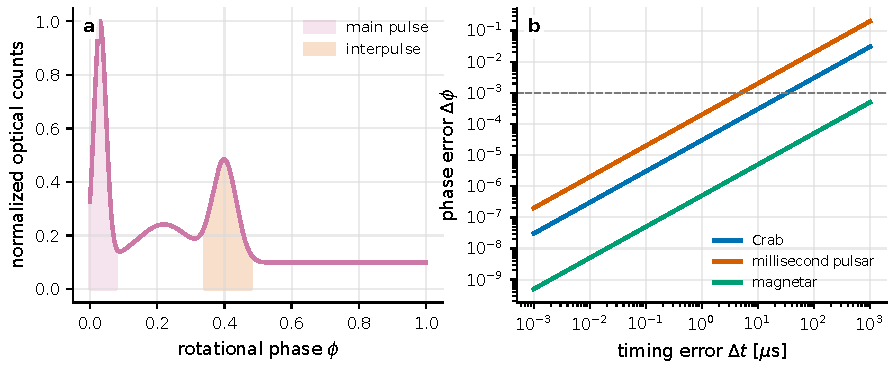
\includegraphics[width=0.94\linewidth]{figures/generated/chapter_19/ch19_crab_phase_windows.pdf}
\caption{Crab 型光学脉冲的相位窗与时间误差。左图示意主脉冲、bridge 和 interpulse 三个事件选择窗；右图把时间误差按式 \eqref{eq:e25-pulse-phase} 换成相位误差。对 Crab，微秒级时间已经绰绰有余；对毫秒脉冲星，则要 ns--\(\mu\mathrm{s}\) 级同步才能保住窄相位结构。}
\label{fig:e25-crab-phase}
\end{figure}

再说\textbf{自然激光}（natural / astrophysical laser）候选。这类目标要检验的是一个很纯粹的量子问题：\textbf{这条亮谱线的光子统计，到底是热的还是相干的？}但要小心一个陷阱——"看到一条亮谱线"本身\textbf{不足以}断言是激光，因为多个互不相干的热模式叠加也能让聚束（bunching）峰被平均掉。定量地说，对 \(M\) 个互不相干的热模式，
\begin{equation}
  g^{(2)}(0)-1
  =
  \frac{1}{M},
  \label{eq:e25-mode-bunching}
\end{equation}
\begin{formulaexplain}
\(M\) 是探测里叠加的互不相干热模式数，\(g^{(2)}(0)\) 是零延迟二阶相干。单模热光有 \(g^{(2)}(0)=2\)（聚束），但 \(M\) 越大，聚束峰被越平均掉，\(g^{(2)}(0)\to1\)。所以 \(g^{(2)}(0)\) 接近 1 并不必然说明光是理想激光。
\end{formulaexplain}
对照记住第 \ref{chap:e08} 章两个极端：单模热态 \(g^{(2)}(0)=2\)、理想相干态（coherent state）\(g^{(2)}(0)=1\)。式 \eqref{eq:e25-mode-bunching} 说的是"多模热光会伪装成相干光"，所以做这类检验必须配一个\textbf{零假设检验}（null test）——把模式数、仪器时间响应、连续谱背景都算清楚，才能判断 \(g^{(2)}(0)\) 偏离 1 或接近 1 意味着什么。另一个可用的把手是谱线宽度：若线宽为 \(\Delta\nu\)，相干时间约 \(\tau_c\sim1/(\pi\Delta\nu)\)（第 \ref{chap:e02} 章带宽--相干时间关系的具体化）。举例，若一条自然激光线窄到 \(\Delta\nu\sim1\,\mathrm{GHz}\)，则 \(\tau_c\sim1/(\pi\times10^9)\approx3\times10^{-10}\,\mathrm{s}=0.3\,\mathrm{ns}\)；线越窄、相干时间越长，在给定探测器时间分辨率下越容易保留可解析的相关\textbf{对比度}（contrast）。真实候选里，Eta Carinae 的 Weigelt blobs 中 Fe II 线被 \(\mathrm{Ly}\alpha\) 泵浦（pumping），Johansson 与 Letokhov 讨论过 \(0.9\text{--}1.0\,\mu\mathrm{m}\) 及近红外的 Fe II 激光线；线宽测量加光子相关谱学（photon-correlation spectroscopy）可以给出直接证据 \citep{2004A&A...428..497J,2005NewA...10..361J,2008AIPC..984..216D}。

\begin{figure}[tbp]
\centering
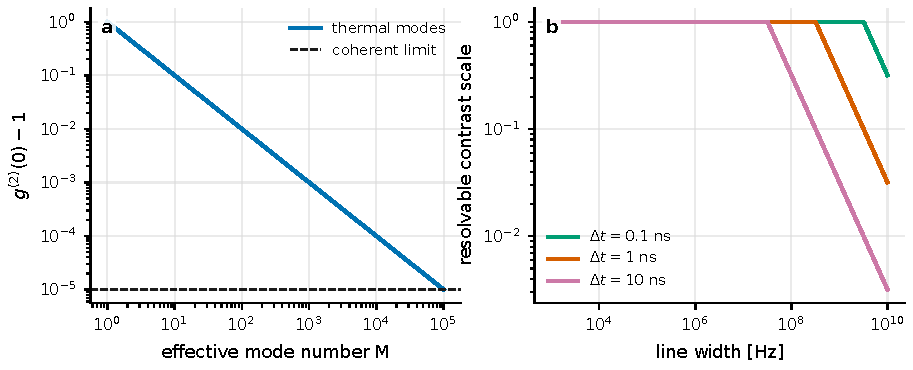
\includegraphics[width=0.94\linewidth]{figures/generated/chapter_19/ch19_natural_laser_statistics.pdf}
\caption{自然激光候选的两个统计判据。左图显示热光模式数 \(M\) 增大会把聚束峰按式 \eqref{eq:e25-mode-bunching} 压低，逼近相干极限 \(g^{(2)}(0)-1=0\)；右图显示线宽越窄、相干时间越长，在给定时间分辨率下越容易保留可解析对比度。二者说明：判断"是否激光"需要联合光子统计与线宽，并做严格的零假设检验。}
\label{fig:e25-natural-laser}
\end{figure}

\textbf{要什么、答什么？}这两类案例更依赖\textbf{事件表质量}——绝对时间同步、精确星历、可验证的背景扣除、以及能分离谱线与连续谱的窄带筛选；它们回答的是"这束光的量子统计是什么性质"，把辐射机制（第 \ref{chap:e16} 章）从光谱层面推到光子统计层面。

\section{把清单排成路线：顺序随仪器成熟而变}
\label{sec:e25-roadmap}

把上面所有案例摆进同一张矩阵，第一代的推进顺序主要由\textbf{技术成熟度}和\textbf{系统风险}决定，而不是纯凭科学价值。图 \ref{fig:e25-priority} 就是这张矩阵：横轴是技术成熟度、纵轴是科学回报、点越大表示系统与触发风险越高。

\begin{figure}[!htbp]
\centering
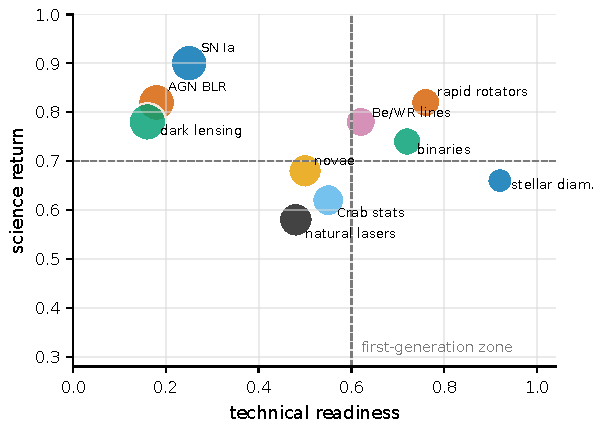
\includegraphics[width=0.78\linewidth]{figures/generated/chapter_19/ch19_priority_matrix.pdf}
\caption{第一代科学案例矩阵。横轴技术成熟度、纵轴科学回报，点越大代表系统误差与触发风险越高。右上方且点较小的目标最适合作为第一代验收；左上方目标（Type Ia、AGN 宽线区、暗物质小尺度透镜）科学价值高，却需要专用阵列或更成熟的量子资源，属长期目标。}
\label{fig:e25-priority}
\end{figure}

读法是这样的：\textbf{右上且点小}的目标（亮热星角直径、已知直径的参考星、\(\beta\) UMa 类 A 型星、MAGIC/VERITAS 可重复目标）风险低、能复现，天然是第一批验收项目；在同一套能力上继续增加科学信息的，是 \(\gamma\) Cas 类快速自转、Be/WR 谱线区、密近双星和新星早期膨胀；更依赖事件表质量与时间/光谱筛选的，是 Crab 相位分辨统计和自然激光候选线；而左上方那些高价值目标——Type Ia 几何距离、AGN 宽线区、暗物质小尺度透镜、量子网络辅助成像（第 \ref{chap:e24} 章）——则应稳稳放在长期目标里。

下面这张表把七类案例的第一观测量、典型数量级和"能不能算第一代"的判据并排列出，便于对照。它其实就是把式 \eqref{eq:e25-priority-score} 那套排序落成一份可执行清单：

\begin{longtable}{p{0.17\linewidth}p{0.22\linewidth}p{0.23\linewidth}p{0.20\linewidth}}
\toprule
案例 & 第一观测量 & 典型数量级 & 第一代判据 \\
\midrule
亮星角直径 & \(|V|^2(B)\) & \(m_V<5\)，\(\theta=0.5\text{--}2\,\mathrm{mas}\) & 多夜重复到 \(3\text{--}5\%\) 直径精度。 \\
快速自转 & 多位置角 \(|V|^2\) & 轴比 \(1.1\text{--}1.5\)，\(\theta<1\,\mathrm{mas}\) & 能区分圆盘与椭圆模型。 \\
双星 & \(|V|^2\) 振荡 & 分离 \(0.2\text{--}5\,\mathrm{mas}\)，\(f>0.1\) & 已有轨道先验，覆盖两个以上位置角。 \\
Be/WR 谱线 & 谱线/连续谱 \(|V|^2\) & \(\mathrm{H}\alpha\)、He、Fe 线 & 线通量足够，连续谱扣除可验证。 \\
新星 & \(\theta(t)\) & 几天后 mas 量级 & 触发快，能与谱线速度合并。 \\
Crab 统计 & 相位窗 \(g^{(2)}\)、颜色相关 & \(P=33\,\mathrm{ms}\) & 星历、背景星云与绝对时间闭合。 \\
自然激光 & \(g^{(2)}\)、线宽、偏振 & \(\Delta\nu\) 可窄到高相干时间 & 谱线可与连续谱分离，有零假设检验。 \\
Type Ia & \(|V|^2(\lambda,t)\) & \(m<12\)，几十 \(\mu\mathrm{as}\) & 公里级阵列与快速触发成熟后再做。 \\
\bottomrule
\end{longtable}

排序会随仪器状态动态改变，这一点很重要。系统刚完成时间同步和零基线相关标定时，亮星角直径和参考星复现最有价值；当六条以上基线能稳定运行、uv 覆盖变好，快速自转和双星进入主清单；当窄带滤光和高数据吞吐可靠，自然激光和谱线盘才有现实空间；只有当阵列扩到公里级、并能每年快速响应 \(m\lesssim12\) 的近邻瞬变时，Type Ia 几何距离才会升为第一线目标 \citep{2017MNRAS.472.4126G,2022MNRAS.512.1722K,2024MNRAS.529.4387A,2024ApJ...966...28A,2025ApJ...995..191A,2025PhRvD.111h3047K}。所有这些取舍，最终都要回到第 \ref{chap:e15} 章的误差预算里去逐条核账——这也是下一部分教学与计算实验（第 \ref{chap:e26} 章）要带你亲手跑一遍的东西。

\section*{本章要点}
\addcontentsline{toc}{section}{本章要点}

\begin{itemize}
  \item \textbf{先排序，再观测。} 用亮度、角尺度、外部先验三把尺子给案例分诊，写成排序式 \eqref{eq:e25-priority-score}：科学回报、技术成熟度、先验提分，系统与触发风险减分。第一代要挑"右上舒服区"的目标，别被漂亮题目牵着走。
  \item \textbf{角直径是第一代最成熟的产品。} 它经均匀圆盘/边缘昏暗模型直接进入有效温度式 \eqref{eq:e25-teff}，且 \(T_{\rm eff}\propto\theta^{-1/2}\) 让 \(4\%\) 的直径误差只传成 \(2\%\) 的温度误差。VERITAS、MAGIC 已在成批出数据。
  \item \textbf{从"多大"到"什么形状"。} 快速自转星要用椭圆可见度式 \eqref{eq:e25-elliptical-visibility}，且必须覆盖多个位置角才能钉住轴比与位置角；\(\gamma\) Cas 已被测出接近临界自转。
  \item \textbf{双星与谱线盘靠基线分辨。} 双星的 \(|V|^2\) 按式 \eqref{eq:e25-binary-visibility} 振荡，振幅 \(2f/(1+f)^2\) 随流量比迅速变小；谱线与连续谱按通量加权混合（式 \eqref{eq:e25-line-continuum}），必须先分离再解释。
  \item \textbf{膨胀瞬变分远近。} 角膨胀式 \eqref{eq:e25-expansion} 给出膨胀视差：银河系新星几天就到 mas，是现实目标；\(10\,\mathrm{Mpc}\) 的 Type Ia 只有几十 \(\mu\mathrm{as}\)，是需要公里级阵列的长期目标。
  \item \textbf{光子统计检验"非热"。} Crab 用相位窗式 \eqref{eq:e25-pulse-phase} 做相位分辨 \(g^{(2)}\)；自然激光要用多模关系式 \eqref{eq:e25-mode-bunching} 加线宽做零假设检验，因为多模热光会伪装成相干光。
  \item \textbf{顺序随仪器成熟而变。} 从零基线标定、到多基线、到窄带高吞吐、再到公里级快响应，路线图是动态的，最终都要回到第 \ref{chap:e15} 章误差预算逐条核账。
\end{itemize}

\medskip
\noindent\textbf{想一想}
\begin{itemize}
  \item 若某亮星角直径测到 \(3\%\) 精度，且总辐射流量 \(F_{\rm bol}\) 也有 \(3\%\) 的独立误差，用式 \eqref{eq:e25-teff} 估一下有效温度 \(T_{\rm eff}\) 的相对误差大约多少？（提示：先分别求 \(T\) 对 \(\theta\) 和对 \(F\) 的对数灵敏度，再按独立误差平方相加。）
  \item 一对流量比 \(f=0.05\) 的双星，用式 \eqref{eq:e25-binary-visibility} 算它 \(|V|^2\) 振荡的余弦振幅是多少？要在 \(1\) 小时内把它测出来，对光子对数和系统校准提出了什么要求（回顾第 \ref{chap:e15} 章）？
  \item 为什么"看到一条又亮又窄的谱线"还不足以断定它是自然激光？式 \eqref{eq:e25-mode-bunching} 里的 \(M\) 在这个判断里扮演什么角色，你会设计一个怎样的零假设检验来排除"多模热光伪装"？
\end{itemize}

\chapter{教学实验与计算实验}
\label{chap:e26}

\begin{chapteropening}
到这里为止，我们已经把整套语言搭好了：光子的到达是随机点过程（第 \ref{chap:e03} 章），热光会\textbf{聚束}、相干光不聚束（第 \ref{chap:e08} 章），两台望远镜之间的空间相干度就是天体亮度分布的可见度（第 \ref{chap:e10}、\ref{chap:e11} 章），而有些参数的信息根本不在你最习惯看的那张图里（第 \ref{chap:e12} 章）。这些道理讲一遍是一回事，\textbf{亲手把它算出来、看见它、并且知道哪里会骗你}，是另一回事。本章就是那间实验室。我们不给出一堆可以直接跑的代码，而是把每一个关键概念拆成一条\textbf{可复算的实验链}：从一张模拟的光子事件表出发，看它怎样变成统计量，统计量怎样进入物理模型，模型的误差又怎样反过来逼你重新设计实验。沿途你会用模拟数据亲眼验证泊松分布和聚束、数值演示 SPADE 如何越过瑞利极限、拟合均匀圆盘和双星的可见度，最后把这些零件拼成一个 Type Ia 超新星测距的玩具模型。每个实验都配一句"常见的坑"，因为在这一行里，一条太漂亮的曲线往往不是好消息，而是一个还没被发现的错误。
\end{chapteropening}

\section{事件表：所有计算实验共用的底稿}
\label{sec:e26-eventtable}

先建立画面。做这一章所有实验的起点，都是一张\textbf{事件表}（event table）——它不是什么高深的数据结构，就是一张表，每一行记一个光子：它什么时候到（时间戳 \(t_i\)）、落在哪个探测器或哪个通道、偏振是什么、以及一个"质量标记"\(q_i\) 说明这个光子可不可信（是不是落在死时间附近、有没有被云挡、电子学有没有饱和）。第 \ref{chap:e13} 章讲过为什么要这么存：一旦你先把光子按时间粗分箱、连成一条平滑的\textbf{光变曲线}（light curve），你就再也无法回头重新选时间窗、重新按偏振或能道筛选、重新做时间平移的背景估计了。分箱是一种\textbf{有损压缩}。事件表则把光场的随机性原封不动地留在硬盘上。

真实的光子计数仪器正是这么工作的。AQuEye、IquEye 这类设备把每个光子都保留成一个时间标签，时间分辨率可到几十皮秒，绝对时间靠 GPS 或原子钟约束到纳秒乃至亚纳秒；像 Timepix 这样的像素计数芯片还能让每一行同时带上空间位置和能量信息 \citep{2016SPIE.9907E..0NZ,2015SPIE.9504E..0CZ,2007NIMPA.581..485L}。所以本章的第一条纪律是：\textbf{实验从事件表开始，不从光变曲线开始}。

如果你确实只关心光变曲线，那也很简单——把事件表按时间 bin 投影一下就行：
\begin{equation}
  n_k=\sum_i \mathbf 1\!\big(t_i\in[t_k,\,t_k+\Delta t)\big)\,\mathbf 1\!\big(q_i=1\big).
  \label{eq:e26-binned-count}
\end{equation}
\begin{formulaexplain}
\(n_k\) 是第 \(k\) 个时间箱里"通过质量筛选"的光子数。两个指示函数 \(\mathbf 1(\cdot)\) 像两道闸门：第一道检查光子到达时刻是否落进这个箱，第二道检查这个光子质量是否合格（\(q_i=1\) 才放行）。求和就是数一数有几个光子同时通过两道闸门。
\end{formulaexplain}
逐个符号落实单位与量纲。\(n_k\) 是一个纯计数，没有量纲；\(\Delta t\) 是箱宽（单位 s），桌面实验常取纳秒到毫秒，天文计时可以从纳秒一路到分钟；\(\mathbf 1(A)\) 是指示函数，条件 \(A\) 成立取 1、否则取 0。想把它变成光子率，只需 \(r_k=n_k/\Delta t\)，单位是 \(\mathrm{s^{-1}}\)。这里已经埋了一个坑：当每箱平均只有几个到几十个光子时，计数涨落是泊松型的，\textbf{不能}随手用对称的高斯误差棒替代；要等到 \(n_k\gtrsim30\)，高斯近似才大致可用。式 \eqref{eq:e26-binned-count} 看起来平淡，但它是本章每一个实验的第一步：先有事件表，再决定投影成什么。

\begin{figure}[tbp]
\centering
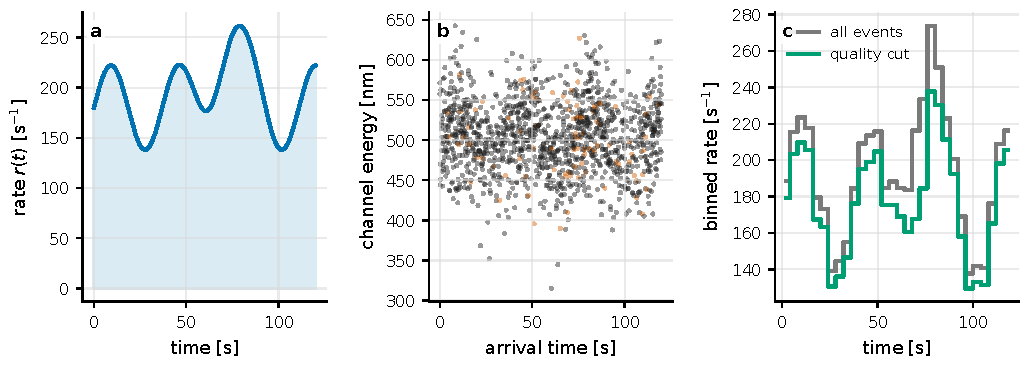
\includegraphics[width=0.96\linewidth]{figures/generated/chapter_20/ch20_event_table_simulation.pdf}
\caption{用非齐次泊松过程生成的模拟事件表。左图是输入光子率 \(r(t)\)；中图保留每个光子的到达时间、等效波长通道和质量标记；右图把事件表投影成光变曲线，并显示质量筛选的影响。事件表比光变曲线多留了通道与质量信息，因此同一份数据还能重新拿去做相关、偏振或能谱分析。}
\label{fig:e26-eventtable}
\end{figure}

\section{第一个计算实验：造一张事件表，验证泊松与散粒噪声}
\label{sec:e26-poisson}

第一个实验的目标最朴素，却最重要：\textbf{亲手造出一张符合泊松统计的事件表，再用它把泊松统计验证回来}，从而彻底吃透第 \ref{chap:e03} 章的散粒噪声。

先说"怎么造"。若光子率恒定为 \(r\)，最省事的办法是利用泊松过程的一个性质：相邻两个光子的时间间隔服从指数分布，\(P(\Delta t)=r\,e^{-r\Delta t}\)。于是从一个均匀随机数 \(u\in(0,1)\) 取 \(\Delta t=-\ln(u)/r\)，一个接一个累加，就得到一串到达时刻。如果率是随时间变的 \(r(t)\)（比如图 \ref{fig:e26-eventtable} 左图那种起伏），就用\textbf{稀释法}（thinning）：先按一个高于所有时刻的常率 \(r_{\max}\) 生成候选光子，再对每个候选以概率 \(r(t_i)/r_{\max}\) 独立地"留下或丢弃"。留下的那些，就是非齐次泊松过程的一次真实实现。这个方法的好处是它逼你把"随机性从哪来"想清楚，而不是调一个黑箱函数。

现在验证。恒定率下，落在长度 \(\Delta t\) 的箱里的光子数 \(N\) 服从泊松分布，这是第 \ref{chap:e03} 章的已知结果，直接点名使用：
\begin{equation}
  P(N)=\frac{\mu^{N}}{N!}\,e^{-\mu},\qquad \mu=r\,\Delta t .
  \label{eq:e26-poisson-pmf}
\end{equation}
\begin{formulaexplain}
\(P(N)\) 是一个箱里恰好数到 \(N\) 个光子的概率，\(\mu\) 是这个箱的\textbf{平均}光子数（等于率乘箱宽）。泊松分布只由一个参数 \(\mu\) 决定，它同时是均值也是方差——这是它最好用、也最好检验的性质。
\end{formulaexplain}
落实符号：\(N\) 是无量纲计数，\(\mu=\bar N\) 是无量纲的平均计数，\(r\) 单位 \(\mathrm{s^{-1}}\)，\(\Delta t\) 单位 s。泊松分布最能被一眼验证的地方，是它的均值与方差\textbf{相等}。我们把这一点写成一个可以直接从数据算的检验量——\textbf{法诺因子}（Fano factor）：
\begin{equation}
  F=\frac{\operatorname{Var}(N)}{\langle N\rangle}\;\xrightarrow[\text{泊松}]{}\;1 .
  \label{eq:e26-fano}
\end{equation}
\begin{formulaexplain}
\(\langle N\rangle\) 是各箱计数的样本均值，\(\operatorname{Var}(N)\) 是它们的样本方差。法诺因子 \(F\) 就是两者之比。纯泊松（相干光、散粒噪声主导）给出 \(F=1\)；聚束的热光会让 \(F>1\)，反聚束的非经典光会让 \(F<1\)。
\end{formulaexplain}
为什么泊松的方差恰好等于均值？这不是巧合，值得当场点名推一遍。由式 \eqref{eq:e26-poisson-pmf}，
\[
  \langle N\rangle=\sum_{N=0}^{\infty}N\,\frac{\mu^N}{N!}e^{-\mu}
  =\mu\,e^{-\mu}\sum_{N=1}^{\infty}\frac{\mu^{N-1}}{(N-1)!}
  =\mu\,e^{-\mu}\,e^{\mu}=\mu,
\]
其中用到了\textbf{几何级数式的指数展开} \(\sum_{m\ge0}\mu^m/m!=e^{\mu}\)（把 \(m=N-1\) 换元即得）。同理算二阶阶乘矩：
\[
  \langle N(N-1)\rangle=\sum_{N=0}^{\infty}N(N-1)\frac{\mu^N}{N!}e^{-\mu}
  =\mu^2 e^{-\mu}\sum_{N=2}^{\infty}\frac{\mu^{N-2}}{(N-2)!}=\mu^2 .
\]
于是 \(\langle N^2\rangle=\langle N(N-1)\rangle+\langle N\rangle=\mu^2+\mu\)，代入方差定义：
\[
  \operatorname{Var}(N)=\langle N^2\rangle-\langle N\rangle^2=(\mu^2+\mu)-\mu^2=\mu .
\]
方差等于均值，一步不跳。这就是散粒噪声那句名言"\(\sigma_N=\sqrt{\bar N}\)"的来处，也是式 \eqref{eq:e26-fano} 里 \(F\to1\) 的根据。

数量级落地：若你造的事件表平均率 \(r=5\times10^{5}\,\mathrm{s^{-1}}\)、箱宽 \(\Delta t=1\,\mathrm{ms}\)，则每箱 \(\mu=500\) 个光子，相对涨落 \(1/\sqrt{\mu}\simeq4.5\%\)；把箱宽缩到 \(1\,\mu\mathrm{s}\)，\(\mu=0.5\)，绝大多数箱是空的，法诺检验要靠大量箱的统计才稳。\textbf{常见的坑}：如果你算出 \(F\) 明显偏离 1，先别急着宣布看到了非经典光——更可能是探测器\textbf{死时间}（dead time）在作怪。死时间会在一个光子之后短暂"致盲"，压低紧挨着的计数，从而人为地把方差压到均值以下（\(F<1\)），伪装成反聚束。所以这个最基础的实验，其实是在教你分辨"物理"和"仪器"。

\section{桌面 HBT：从随机符合里"看见"聚束}
\label{sec:e26-hbt}

第二个实验把泊松推进到\textbf{二阶}：用一束光、一个分束器、两个探测器，做一次桌面版的汉伯里·布朗–特维斯（Hanbury Brown--Twiss, HBT）实验，亲手测出 \(g^{(2)}(\tau)\)，验证第 \ref{chap:e08} 章的聚束 \citep{1956Natur.178.1046H,1957RSPSA.242..300B,1963PhRv..130.2529G}。

先要画面。两路强度各自都在随机跳动，凭什么零延迟附近会比别处多一点"共同的"起伏？把热光（或旋转毛玻璃造出的\textbf{伪热光}, pseudothermal light）想成许多相位随机的模式叠加，它的瞬时强度并不平，而是忽高忽低。在同一个\textbf{相干时间} \(\tau_c\) 之内，这一次强度涨落是被两个探测器\textbf{共享}的——强度高的那一瞬，两边同时更容易各接到一个光子，于是"符合"（coincidence）在 \(\tau=0\) 附近增多。激光是例外：它每个模式相位锁定，强度平得像一潭死水，所以 \(g^{(2)}(0)\simeq1\)，不聚束 \citep{1991PhRvL..67.1426N,1999PhRvA..60..674B,2024arXiv240418606N}。

怎么从事件表把它算出来？做法是数\textbf{符合对}并归一化。把两路事件表按时间差 \(\tau=t_j^{(2)}-t_i^{(1)}\) 统计成一个延迟直方图 \(H(\tau)\)，再除以一个"本该如此"的随机基线：
\begin{equation}
  \hat g^{(2)}(\tau)=\frac{H(\tau)}{H_{\rm bg}(\tau)},\qquad
  H_{\rm bg}\simeq R_1 R_2\,T\,\Delta\tau .
  \label{eq:e26-g2-estimator}
\end{equation}
\begin{formulaexplain}
\(H(\tau)\) 是时间差落在第 \(\tau\) 个延迟箱里的光子对数目。\(H_{\rm bg}\) 是"如果两路完全独立"时该有的偶然符合数：两路率 \(R_1,R_2\) 相乘、乘总时长 \(T\)、再乘延迟箱宽 \(\Delta\tau\)。相除就把仪器的绝对计数抵掉，只留下\textbf{相对}于随机符合的超额。
\end{formulaexplain}
落实符号：\(R_1,R_2\) 是两路单计数率（\(\mathrm{s^{-1}}\)），\(T\) 是总积分时间（s），\(\Delta\tau\) 是延迟箱宽（s），\(H,H_{\rm bg}\) 都是无量纲计数。分母 \(H_{\rm bg}\) 有一个更靠谱的实测版本：把第二路整体\textbf{时间平移}一个远大于 \(\tau_c\) 的量再数一遍符合——那时物理相关早已消失，剩下的纯是偶然，这就是\textbf{time-shift 背景}。用它归一化，能自动吸收慢漂移。

数量级要让人心里有底。取 \(R_1=R_2=5\times10^{5}\,\mathrm{s^{-1}}\)、\(T=300\,\mathrm{s}\)、\(\Delta\tau=0.5\,\mathrm{ns}\)，则每个延迟箱的随机符合约
\[
  H_{\rm bg}\simeq (5\times10^5)^2\times300\times(0.5\times10^{-9})\approx3.75\times10^{4}\ \text{对/箱}.
\]
这些对数本身是泊松涨落的，散粒相对误差约 \(1/\sqrt{H_{\rm bg}}\simeq5\times10^{-3}\)。于是一个 \(g^{(2)}-1\sim10^{-2}\) 的峰在桌面上抬头可见——而这正是问题所在。

\begin{figure}[tbp]
\centering
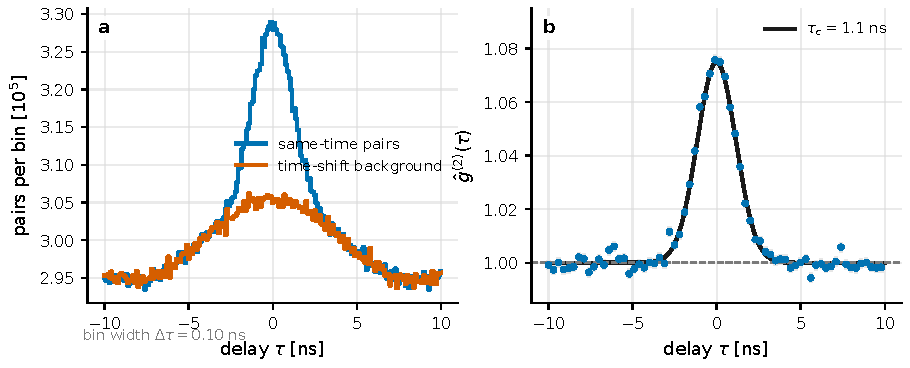
\includegraphics[width=0.96\linewidth]{figures/generated/chapter_20/ch20_hbt_lab_histogram.pdf}
\caption{桌面 HBT 的延迟直方图。左图比较同时时间轴上的"对/箱"与 time-shift 背景；慢漂移会同时出现在两条曲线里，因此被归一化抵掉。右图用背景直方图归一化后得到 \(\hat g^{(2)}(\tau)\)，零延迟附近的峰宽由光源相干时间与探测器响应共同决定。}
\label{fig:e26-hbt}
\end{figure}

\textbf{最要命的坑：对比度稀释。}真实仪器测到的不是理想 \(g^{(2)}\)，而是它被探测器时间响应\textbf{卷积}后的样子。若相干时间 \(\tau_c\) 远小于电子学响应宽度或延迟箱宽 \(\Delta\tau\)，热光本该到 2 的峰会被稀释，观测对比度近似按 \(\tau_c/\Delta\tau\) 缩小。算给你看：一片中心 \(416\,\mathrm{nm}\)、带宽 \(\Delta\lambda=13\,\mathrm{nm}\) 的窄带滤光片，带宽换算 \(\Delta\nu\simeq c\,\Delta\lambda/\lambda^2\approx2.3\times10^{13}\,\mathrm{Hz}\)，相干时间 \(\tau_c\simeq1/\Delta\nu\approx4\times10^{-14}\,\mathrm{s}\)；用几纳秒的电子学去采样，对比度被压到 \(\tau_c/\Delta\tau\sim10^{-5}\) 量级。这就是为什么桌面上若看到一个又高又漂亮的峰，你的第一反应\textbf{不应该}是高兴，而应该是追问：它到底来自单模热光，还是电子学串扰、光源慢漂移、或者归一化选得太巧？VERITAS、MAGIC、Asiago 的强度干涉分析无一例外都要显式处理这份稀释、背景与死时间账本 \citep{2009A&A...508..531N,2020NatAs...4.1164A,2024MNRAS.529.4387A,2017MNRAS.472.4126G}。这也顺带解释了下一节的分工：桌面能看见的 \(10^{-2}\) 峰，和天文上要抠的 \(10^{-5}\) 峰，差着五个数量级。

\section{从桌面到长基线：模拟并拟合均匀圆盘的可见度}
\label{sec:e26-disk}

把 HBT 从桌面搬到\textbf{两台望远镜}之间，它就成了强度干涉仪（第 \ref{chap:e10} 章）。物理没变——仍然是比较两路强度起伏是否同步——但现在两台望远镜看的是同一颗\textbf{有角大小}的星。基线越长，两个孔径看到的相干涨落越不一样，零延迟峰就越低。这份"随基线下降"的曲线，正是天体亮度分布的可见度。

第 \ref{chap:e08} 章的 Siegert 关系告诉我们，二阶相关的超额等于一阶相干度的模平方；第 \ref{chap:e10} 章的 van Cittert--Zernike 定理又告诉我们，两台望远镜之间的一阶空间相干度 \(\gamma_{12}\) 就是天体归一化亮度分布的傅里叶变换，即可见度 \(V\)。把两者接起来，实验上从数据估计 \(|V|^2\) 的流程是这样的：每条基线 \(b\) 先给出零延迟的过量相关 \(\hat c_b=\hat g^{(2)}_b(0)-1\)，再用当夜的标定星（或实验室标定）测得的仪器对比度 \(\hat\beta_b\) 去除：
\begin{equation}
  \widehat{|V_b|^2}=\frac{\hat c_b}{\hat\beta_b}.
  \label{eq:e26-v2-estimator}
\end{equation}
\begin{formulaexplain}
\(\hat c_b\) 是基线 \(b\) 测到的零延迟相关超额，\(\hat\beta_b\) 是同一条基线的仪器对比度（把时间响应、带宽、偏振选择、效率造成的稀释一并收进去）。两者相除才剥出天体自己的 \(|V_b|^2\)。注意：\(\beta\) 出现在\textbf{分母}，所以它的标定误差会被\textbf{直接放大}进结果。
\end{formulaexplain}
\(\hat c_b\)、\(\hat\beta_b\)、\(|V_b|^2\) 都是无量纲量。若某基线的随机符合数为 \(H_b\)、系统误差暂忽略，则 \(\sigma_{\hat c}\simeq H_b^{-1/2}\)；可一旦真实对比度小到 \(\beta\sim10^{-5}\)，同样的 \(\sigma_{\hat c}\) 就被放大成 \(\sigma_{|V|^2}\simeq\sigma_{\hat c}/\beta\)。\textbf{教学模拟的坑正在这里}：为了让信号在图上看得见，你会忍不住把 \(\beta\) 取到 \(0.05\) 这种"友好"的值，于是得到一个假装很干净的 \(g^{(2)}\) 峰；但真实天文 \(|V|^2\) 的精度，仍然由那个 \(10^{-6}\)–\(10^{-5}\) 的真实对比度、随机符合数和系统地板决定。做模拟时把这个放大因子写在报告最显眼处，是基本诚实。

现在造数据、做拟合。最常用的源模型是\textbf{均匀圆盘}（uniform disk），它的可见度是第 \ref{chap:e11} 章的已知结果，直接点名：
\begin{equation}
  V(B_\perp)=\frac{2J_1(x)}{x},\qquad
  x=\frac{\pi\,\theta\,B_\perp}{\lambda},
  \label{eq:e26-uniform-disk}
\end{equation}
\begin{formulaexplain}
\(V\) 是可见度，\(J_1\) 是一阶贝塞尔函数，\(x\) 是把角直径、基线、波长揉成的一个无量纲组合。\(x\) 越大（基线越长或星越大），\(V\) 越小；\(2J_1(x)/x\) 在 \(x\to0\) 时趋于 1，第一次归零发生在 \(x=3.8317\)。观测里能拿到的是 \(|V|^2\)，相位信息在强度干涉里丢了符号。
\end{formulaexplain}
逐个落实：\(\theta\) 是角直径（rad，报告里常写 mas 或 \(\mu\mathrm{as}\)），\(B_\perp\) 是投影基线（m），\(\lambda\) 是观测波长（m），\(J_1\) 无量纲。把第一零点 \(x=3.8317\) 代进去，得到最能定角直径的那条基线：
\[
  B_{\rm null}=\frac{3.8317}{\pi}\,\frac{\lambda}{\theta}\approx1.22\,\frac{\lambda}{\theta}.
\]
代真实数字：\(\lambda=416\,\mathrm{nm}\)、\(\theta=1\,\mathrm{mas}=4.85\times10^{-9}\,\mathrm{rad}\)，
\[
  B_{\rm null}\approx1.22\times\frac{416\times10^{-9}}{4.85\times10^{-9}}\ \mathrm{m}\approx105\,\mathrm{m}.
\]
这一个数就解释了整片版图：\(1\,\mathrm{mas}\) 亮星的第一零点落在百米级基线，所以 VERITAS 这类百米级切伦科夫阵列能测亮星角直径；而 Type Ia 超新星那几个 \(\mu\mathrm{as}\) 的角半径，第一零点要退到几十公里以外，只能靠公里级基线。拟合时的\textbf{要点}是：\(|V|^2\) 对 \(\theta\) 最敏感的地方在第一零点附近的陡坡上，所以基线覆盖若全挤在 \(V\approx1\) 的平台区，后验会很宽；把基线铺到零点两侧，角直径才收得紧。

\begin{figure}[tbp]
\centering
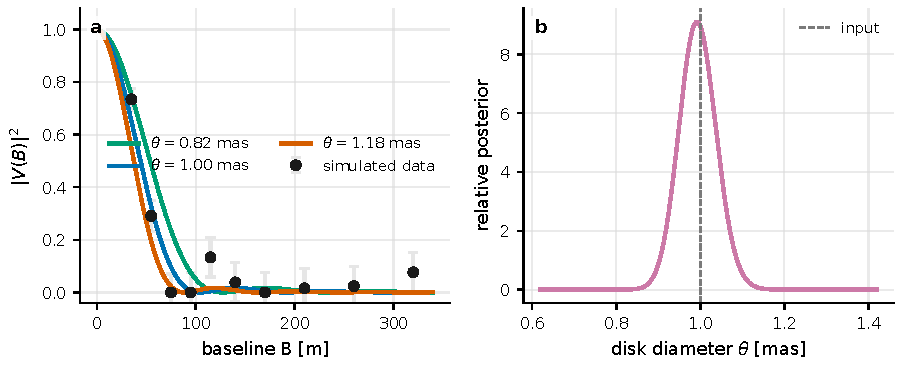
\includegraphics[width=0.96\linewidth]{figures/generated/chapter_20/ch20_uniform_disk_fit.pdf}
\caption{均匀圆盘的强度干涉拟合。左图模拟 \(\lambda=416\,\mathrm{nm}\)、\(\theta=1\,\mathrm{mas}\) 的目标在不同基线上的 \(|V|^2\) 测量，第一零点附近斜率最大、对角直径最敏感。右图把这些数据转成角直径后验，后验宽度由 \(|V|^2\) 误差、基线覆盖和模型假设共同决定。}
\label{fig:e26-disk}
\end{figure}

\section{双星与 uv 覆盖：为什么要多基线、多历元}
\label{sec:e26-binary}

均匀圆盘只有一个参数，双星把故事变有趣：它让你亲眼看到，强度干涉虽然丢了可见度的\textbf{符号}（相位），却仍然保留了随基线振荡的\textbf{空间频率}。两个非相干点源的归一化可见度平方是第 \ref{chap:e10}、\ref{chap:e11} 章的已知结果：
\begin{equation}
  |V(\bm B_\perp)|^2=\frac{1+\rho^2+2\rho\cos\!\big(2\pi\,\bm B_\perp\!\cdot\!\bm s/\lambda\big)}{(1+\rho)^2},
  \label{eq:e26-binary}
\end{equation}
\begin{formulaexplain}
\(\rho=F_2/F_1\) 是伴星与主星的通量比，\(\bm s\) 是两星的角分离向量，\(\bm B_\perp\!\cdot\!\bm s/\lambda\) 是投影到基线方向上的无量纲相位。分子里的余弦项让 \(|V|^2\) 随基线上下振荡，分母 \((1+\rho)^2\) 只是把它归一化到 \(\bm B_\perp\to0\) 时的 1。
\end{formulaexplain}
落实符号与量纲：\(\rho\) 无量纲，\(\bm s\) 是角度向量（rad，报告常用 mas），\(\bm B_\perp\) 单位 m，\(\lambda\) 单位 m，整个 \(\bm B_\perp\!\cdot\!\bm s/\lambda\) 无量纲。看两个极端能体会它在说什么。等亮双星 \(\rho=1\) 时，式 \eqref{eq:e26-binary} 化成 \((1+\cos\phi)/2\)，随相位从 1 一路荡到 0——满调制。若伴星只有主星一成通量 \(\rho=0.1\)，余弦项让 \(|V|^2\) 围绕自己的均值上下摆动，这个\textbf{振荡半幅}为
\[
  \frac{2\rho}{(1+\rho)^2}=\frac{2\times0.1}{1.1^2}\approx0.17,
\]
而摆动的中心（均值）是 \(\dfrac{1+\rho^2}{(1+\rho)^2}=\dfrac{1.01}{1.21}\approx0.835\)。于是 \(|V|^2\) 在均值 \(0.835\) 上下各摆 \(0.17\)，实际是在约 \(0.67\) 到 \(1\) 之间起伏：最大值 \(1\) 出现在 \(\cos\phi=1\)，最小值 \(\dfrac{(1-\rho)^2}{(1+\rho)^2}=\dfrac{0.81}{1.21}\approx0.67\) 出现在 \(\cos\phi=-1\)，峰谷差约 \(0.33\)。伴星越暗，波纹越浅，越考验测量精度。相位也算一个给你看：\(B=180\,\mathrm{m}\)、\(\lambda=500\,\mathrm{nm}\)、分离 \(0.5\,\mathrm{mas}=2.42\times10^{-9}\,\mathrm{rad}\) 时，
\[
  \phi=2\pi\frac{B\,s}{\lambda}=2\pi\times\frac{180\times2.42\times10^{-9}}{500\times10^{-9}}\approx5.5\ \mathrm{rad},
\]
接近一整圈——单条基线上就能看到明显的一个振荡周期。

但一条基线只是 uv 平面上的\textbf{一个点}（第 \ref{chap:e11} 章）。要同时定出分离的大小、方向、通量比和轨道几何，就得铺开 uv 覆盖：多条基线在一个时刻采到不同的 \(\bm B_\perp\)，加上地球自转让每条基线的投影 \(\bm B_\perp(t)\) 在一夜里划出弧线（\textbf{地球自转合成孔径}），多历元又让 \(\bm s(t)\) 随轨道运动扫过不同相位。这就是"多基线、多历元"这句口号的实质：\textbf{用不同的 uv 采样把简并的参数一个个拆开}。\textbf{常见的坑}：若 uv 覆盖只沿一个方向，垂直方向的分离就基本不受约束，拟合会给出一个被拉长的、误导人的误差椭圆——图好看，参数不可信。

\begin{figure}[tbp]
\centering
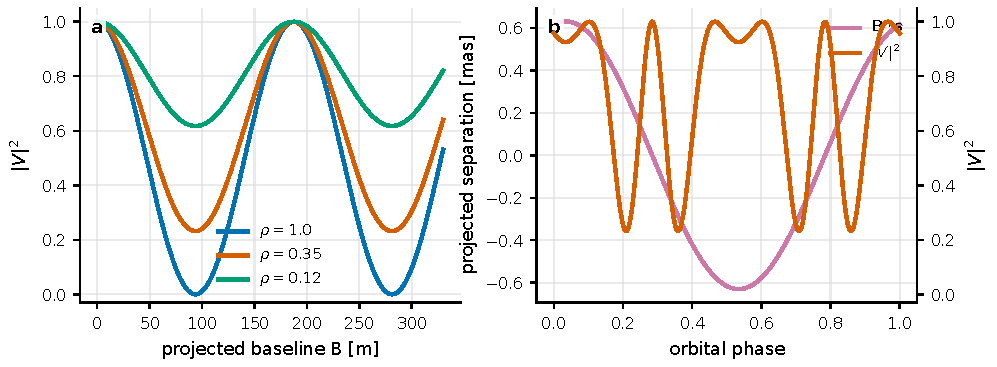
\includegraphics[width=0.96\linewidth]{figures/generated/chapter_20/ch20_binary_visibility.pdf}
\caption{双星 \(|V|^2\) 案例。左图显示固定角分离下，通量比 \(\rho\) 如何控制基线上振荡的深浅；右图显示倾斜轨道中投影分离 \(\bm B\!\cdot\!\bm s\) 随轨道相位变化，从而改变固定基线上的 \(|V|^2\)。多基线与多历元数据用来分开分离、通量比和轨道几何。}
\label{fig:e26-binary}
\end{figure}

\section{相关器：把事件表变成相关函数，并且学会怀疑它}
\label{sec:e26-correlator}

前面几节默默假设"我们已经有了 \(g^{(2)}(\tau)\)"。这一节补上中间那台机器——\textbf{相关器}（correlator）——并且强调它一半的价值在于\textbf{质量控制}，而不是速度。

相关器的任务只有一句话：把两路事件表变成一批延迟直方图，且每一个符合对都必须能追溯回两条原始事件和一个时间差。实现上有三条路，都算同一个量、但代价不同。最朴素的双重循环比较所有事件对，计算量随 \(N_1 N_2\) 增长，慢得离谱。若事件已按时间排序，就只比较落在相关窗口 \(|t_j-t_i|<\tau_{\max}\) 内的邻居，计算量降到约 \(N_\gamma k\)，其中 \(k\sim2R\tau_{\max}\) 是每个光子附近的候选对数。第三条路是先按均匀时间箱把事件投影成序列，再用快速傅里叶变换做互相关，计算量约 \(M\log M\)（\(M=T/\Delta t\)）。三者结果一致，但内存占用、时间分辨和死时间处理各不相同——这本身就是一个好的对照实验。

为什么工程压力这么大？两个标度说明一切。多望远镜阵列的\textbf{基线数}随望远镜数二次增长（第 \ref{chap:e11} 章）：4 台望远镜只有 6 条基线，60 台就有 \(\binom{60}{2}=1770\) 条。单台望远镜的\textbf{原始数据率}则随时间箱变窄、光谱通道增多而膨胀：
\begin{equation}
  D\simeq \frac{N_\nu\,n_{\rm bit}}{\Delta t},
  \label{eq:e26-datarate}
\end{equation}
\begin{formulaexplain}
\(D\) 是单路数据率，\(N_\nu\) 是同时保留的光谱通道数，\(n_{\rm bit}\) 是每个时间箱的比特数，\(\Delta t\) 是时间箱宽。箱越窄、通道越多，数据流越猛——这决定了相关必须靠什么硬件来扛。
\end{formulaexplain}
落实单位：\(D\) 单位 \(\mathrm{bit\,s^{-1}}\)，\(N_\nu\) 无量纲，\(n_{\rm bit}\) 无量纲，\(\Delta t\) 单位 s。代真实数字：\(\Delta t=4\,\mathrm{ns}\)、单通道 \(N_\nu=1\)、\(n_{\rm bit}=16\) 时，\(D\simeq16/(4\times10^{-9})=4\times10^{9}\,\mathrm{bit\,s^{-1}}=4\,\mathrm{Gb\,s^{-1}}\)；若同时留 64 个光谱通道，单台就冲到 \(256\,\mathrm{Gb\,s^{-1}}\)。这就是为什么现代强度干涉离不开 GPU/FPGA 实时相关、分层触发、片上累加或严格压缩——MAGIC 的实时无死时间相关器和 VERITAS 的在线/离线流程都是被这个数据率逼出来的 \citep{2020NatAs...4.1164A,2024MNRAS.529.4387A,2024ApJ...966...28A}。

\begin{figure}[tbp]
\centering
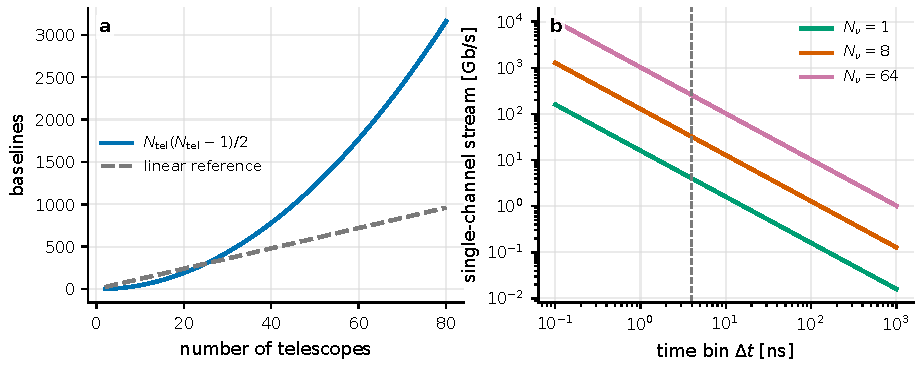
\includegraphics[width=0.96\linewidth]{figures/generated/chapter_20/ch20_correlator_scaling.pdf}
\caption{多望远镜相关器的两个标度。左图：基线数随望远镜数二次增长，阵列一扩就迅速增加相关任务。右图：单路数据流随时间箱变窄和光谱通道增多而上升；纳秒级采样加几十个光谱通道，已进入必须靠实时硬件或 GPU 处理的区域。}
\label{fig:e26-correlator}
\end{figure}

真正把这一节和前面区分开的，是\textbf{null test（零假设检验）}——而且它应该像结果图一样被认真评分，不是附录里的走过场。至少要做这几项：把第二路整体平移远大于 \(\tau_c\) 的时间，真实峰\textbf{必须消失}；盖上遮光片或没有星光时跑同样流程，电子学串扰\textbf{不该}冒出零延迟峰；把偏振或光谱通道打乱，只有物理上该相关的通道保留信号；把数据按时间切片，\(\hat g^{(2)}(0)-1\) 应该随积分时间按 \(T^{-1/2}\) 平稳收敛，而不是集中在某一小段时间里。这些检验直接决定一个峰能不能被解释成天体信号——Guerin 等人的桌面/在天实验、AQuEye/IquEye 的光子计数方案，以及现代切伦科夫阵列的强度干涉，都把它们当成结果的一部分 \citep{2017MNRAS.472.4126G,2016SPIE.9907E..0NZ,2021MNRAS.506.1585Z,2020NatAs...4.1164A}。\textbf{一句话的纪律}：一个通过了 null test 的小峰，比一个没通过 null test 的大峰值钱得多。

\section{数值演示 SPADE：信息不在最亮的像素里}
\label{sec:e26-spade}

现在换一个看似无关、实则同源的实验，呼应第 \ref{chap:e12} 章。前面用长基线去够高空间频率；这里的问题反过来：\textbf{已经成像了，两个点源挨得比点扩散函数还近，还能不能量出它们的分离？}直接成像的答案很沮丧，而模式排序（SPADE）会告诉你信息其实一直都在，只是没在你盯着的那几个亮像素里。

先建立画面。两个等亮、非相干的点源，分离 \(s\) 远小于点扩散函数（point spread function, PSF）宽度 \(\sigma\) 时，焦平面上的合成像几乎只是"稍微胖了一点点"。糟糕的是，像素强度对 \(s\) 的\textbf{导数}在 \(s\to0\) 时趋于零——你想估的参数几乎不改变你测的东西，于是费雪信息（Fisher information）塌向零。这就是\textbf{瑞利诅咒}（Rayleigh curse）在统计上的准确含义：不是"分辨不出"，而是"直接成像这个测量方式，把关于 \(s\) 的信息浪费掉了" \citep{2015Optic...2..646T,2016PhRvX...6c1033T}。

SPADE 换一种测量：不测像素强度，而是把光投影到一组\textbf{厄米–高斯模式}（Hermite--Gaussian modes）上，数每个模式里有几个光子。对高斯 PSF、等亮双点源，这是第 \ref{chap:e12} 章给出的已知结果——落到第 \(n\) 个模式的概率是泊松形的：
\begin{equation}
  p_n=e^{-\Gamma}\,\frac{\Gamma^{\,n}}{n!},\qquad
  \Gamma=\left(\frac{s}{4\sigma}\right)^{\!2}.
  \label{eq:e26-spade-prob}
\end{equation}
\begin{formulaexplain}
\(p_n\) 是一个光子被投影到第 \(n\) 个厄米–高斯模式的概率，\(n=0,1,2,\dots\) 是横向模式编号。\(\Gamma\) 是把分离与 PSF 宽度揉成的无量纲小量。分离越小 \(\Gamma\) 越小，绝大多数光子仍落在基模 \(n=0\)，但 \(n\ge1\) 的那点小概率对 \(s\) 极其敏感。
\end{formulaexplain}
落实符号：\(s\) 是角分离（与 \(\sigma\) 同用一种角单位或同一种焦面长度单位），\(\sigma\) 是 PSF 高斯宽度，\(\Gamma\)、\(p_n\) 无量纲。代数字：\(s=0.2\sigma\) 时 \(\Gamma=(0.2/4)^2=2.5\times10^{-3}\)，于是 \(p_1\approx\Gamma=2.5\times10^{-3}\)，一千个光子里才盼到两三个进 \(n=1\) 模式——但恰恰是这两三个光子扛着几乎全部关于 \(s\) 的信息。

为什么说信息没塌？把泊松概率式 \eqref{eq:e26-spade-prob} 的费雪信息一步步算出来。单个光子对参数 \(s\) 的费雪信息是
\[
  I_{\rm SPADE}(s)=\sum_{n}\frac{1}{p_n}\!\left(\frac{\partial p_n}{\partial s}\right)^{\!2}.
\]
利用泊松分布的一个标准事实——泊松均值 \(\Gamma\) 本身的费雪信息是 \(1/\Gamma\)，再用链式法则 \(I_s=(d\Gamma/ds)^2\cdot(1/\Gamma)\)。代 \(\Gamma=s^2/(16\sigma^2)\)，则 \(d\Gamma/ds=s/(8\sigma^2)\)，于是
\[
  I_{\rm SPADE}(s)=\frac{\big(s/8\sigma^2\big)^2}{s^2/(16\sigma^2)}
  =\frac{s^2/(64\sigma^4)}{s^2/(16\sigma^2)}=\frac{16\sigma^2}{64\sigma^4}=\frac{1}{4\sigma^2}.
\]
一步不跳，结果干净得惊人：\(I_{\rm SPADE}=1/(4\sigma^2)\)，\textbf{与分离 \(s\) 无关}——哪怕 \(s\to0\)，每个光子携带的信息也不衰减。对照之下，直接成像的费雪信息随 \(s\to0\) 塌向零。这就是 SPADE 越过瑞利诅咒的全部秘密。

\begin{figure}[tbp]
\centering
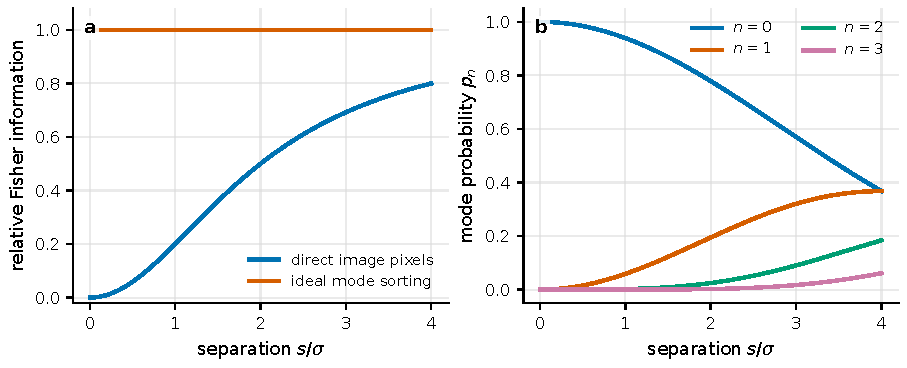
\includegraphics[width=0.96\linewidth]{figures/generated/chapter_20/ch20_spade_computational_experiment.pdf}
\caption{SPADE 计算实验。左图比较小分离处直接像素成像与理想模式排序的相对费雪信息：直接成像在 \(s/\sigma\ll1\) 时信息下降，模式排序保持接近常数。右图显示厄米–高斯模式概率，分离很小时高阶模式概率虽小但斜率非零，因此需要高稳定、低串扰的模式测量。}
\label{fig:e26-spade}
\end{figure}

\textbf{务必写进代码的坑}：上面那条漂亮的常数曲线是\textbf{理想}情形。真实系统里，模式基与真实 PSF 不完全匹配、中心定位有误差、有像差、有背景光——任何一点\textbf{模式串扰}（cross-talk）都会让本该干净的 \(n=1\) 模式漏进一点 \(n=0\) 的光，从而给费雪信息垫一块\textbf{信息地板}，把 \(s\to0\) 的优势削平。所以教学代码不该只画理想曲线，而要加一个可调的串扰参数，让学生看着信息地板随串扰升高而抬起。正因如此，SPADE 目前更适合当作计算实验和先导验证（pathfinder），而不是承诺下一代望远镜就能无损触及量子极限 \citep{2016OExpr..24.3684N,2017PhRvL.118g0801T}。

\section{综合项目：Type Ia 距离玩具模型如何串起整套误差预算}
\label{sec:e26-typeia}

最后一个项目把前面的零件拼成整机，也故意暴露玩具模型最容易掩盖的危险：角半径、速度、爆炸时间看起来只差一个比例常数，真实误差却来自\textbf{不同仪器、不同模型、不同历元}。这就是用膨胀光球法（expanding photosphere method）给 Type Ia 超新星测角直径距离的思路 \citep{2025PhRvD.111h3047K}。

物理链条是这样的：光谱模型给出光球膨胀速度 \(v_{\rm ph}(t)\)，强度干涉给出光球角半径 \(\theta_{\rm ph}(t)\)，两者一比就得到角直径距离：
\begin{equation}
  \theta_{\rm ph}(t)=\frac{R_{\rm ph}(t)}{D_A}\simeq\frac{v_{\rm ph}\,(t-t_0)}{D_A}.
  \label{eq:e26-typeia-theta}
\end{equation}
\begin{formulaexplain}
\(\theta_{\rm ph}\) 是光球角半径，\(R_{\rm ph}\) 是物理半径，\(D_A\) 是角直径距离，\(t_0\) 是爆炸时刻。若光球以近似恒定速度 \(v_{\rm ph}\) 膨胀，则物理半径约为速度乘时间；用它除以角半径，就把距离逼出来了。
\end{formulaexplain}
落实符号与量纲：\(v_{\rm ph}\) 单位 \(\mathrm{cm\,s^{-1}}\)，正常 Type Ia 早期约 \(8\times10^8\)–\(1.5\times10^9\,\mathrm{cm\,s^{-1}}\)；\(t-t_0\) 单位 s 或 d，强度干涉最感兴趣的是爆炸后几天到几十天；\(D_A\) 用 Mpc；\(\theta_{\rm ph}\) 通常几到几十 \(\mu\mathrm{as}\)。代真实数字：\(v_{\rm ph}=10^{9}\,\mathrm{cm\,s^{-1}}\)、\(t-t_0=15\,\mathrm{d}=1.30\times10^{6}\,\mathrm{s}\)，物理半径 \(R_{\rm ph}\approx1.30\times10^{15}\,\mathrm{cm}\)；再取 \(D_A=20\,\mathrm{Mpc}=6.17\times10^{25}\,\mathrm{cm}\)，
\[
  \theta_{\rm ph}\approx\frac{1.30\times10^{15}}{6.17\times10^{25}}\ \mathrm{rad}
  \approx2.1\times10^{-11}\,\mathrm{rad}\approx4.3\,\mu\mathrm{as}.
\]
在 \(\lambda=500\,\mathrm{nm}\) 下，这对应第一零点基线尺度 \(\lambda/\theta\sim24\,\mathrm{km}\)。若肯用整条可见度曲线而不只等第一零点，公里到十公里级基线仍有科学信息可挖——但误差预算会绷得极紧。

怎么把角半径和速度合成一个距离后验？写一个联合似然，同时惩罚"角半径预言"和"速度预言"的不一致：
\begin{equation}
  \ln{\cal L}(D_A)=
  -\frac12\sum_k\!\left[\frac{\hat\theta_k-v_{{\rm ph},k}(t_k-t_0)/D_A}{\sigma_{\theta,k}}\right]^2
  -\frac12\sum_k\!\left[\frac{\hat v_k-v_{{\rm ph},k}}{\sigma_{v,k}}\right]^2 .
  \label{eq:e26-typeia-like}
\end{equation}
\begin{formulaexplain}
\(D_A\) 是待估距离，\(\hat\theta_k\) 与 \(\hat v_k\) 是第 \(k\) 个历元测到的角半径与速度，\(\sigma_{\theta,k}\)、\(\sigma_{v,k}\) 是各自的误差。第一个和式管"角半径要和 \(v(t-t_0)/D_A\) 对上"，第二个和式管"速度模型要和测到的速度对上"。两项一起被最小化，才能同时约束 \(D_A\)。
\end{formulaexplain}
落实符号：\(\hat\theta_k\) 来自第 \(k\) 历元的 \(|V|^2\) 拟合（式 \eqref{eq:e26-v2-estimator}、\eqref{eq:e26-uniform-disk} 那套），单位 rad 或 \(\mu\mathrm{as}\)；\(\hat v_k\) 来自谱线速度或辐射转移模型，单位 \(\mathrm{cm\,s^{-1}}\)；\(\sigma_{\theta,k}\)、\(\sigma_{v,k}\) 各自\textbf{同时}包含统计误差和模型系统误差。\textbf{玩具模型最大的坑}正在这里：如果你偷懒只给 \(\hat\theta\) 加个 \(10\%\) 的高斯噪声，就会得到一个漂亮到失真的窄后验。真实项目必须让学生去动那些"看不见的旋钮"——变动爆炸时间 \(t_0\)、给速度加梯度、放进非球对称、换掉均匀圆盘换成有临边昏暗的亮度分布——然后看着后验一点点变宽。后验\textbf{应该}变宽，那才是诚实的误差预算。

\begin{figure}[tbp]
\centering
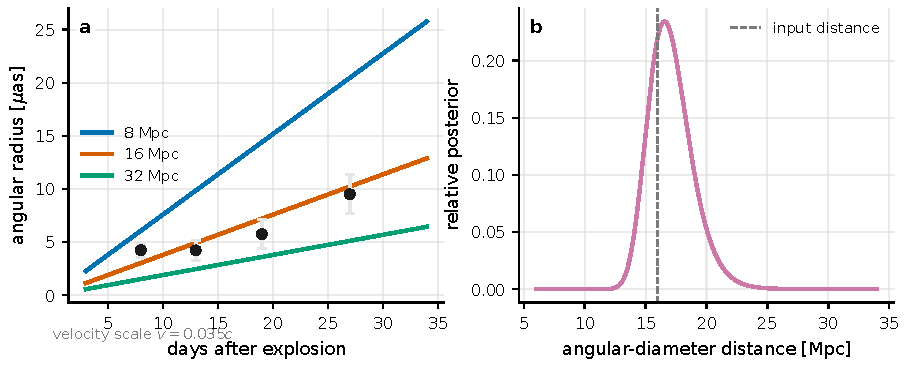
\includegraphics[width=0.96\linewidth]{figures/generated/chapter_20/ch20_typeia_distance_posterior.pdf}
\caption{Type Ia 超新星角直径距离玩具模型。左图用 \(v_{\rm ph}=0.035c\) 的简化膨胀模型，给出不同距离下角半径随时间的变化，并叠加模拟角半径测量；右图把这些角半径与速度模型合成 \(D_A\) 后验。真实分析要用辐射转移模型替代恒速球壳，并把非球对称、谱线形成层和基线覆盖都写进误差预算。}
\label{fig:e26-typeia}
\end{figure}

这五个项目连起来，正好是一条难度递进的课程线：先用 LED、伪热光、激光测 \(g^{(2)}(\tau)\)，验证泊松与聚束；再在同一份事件表上练 time-shift 背景、质量筛选和 \(T^{-1/2}\) 收敛；进入空间相干后拟合均匀圆盘和双星 \(|V|^2\)，体会基线覆盖的作用；然后做 SPADE，看费雪信息如何逃过瑞利诅咒，又如何被串扰按回地板；最后用 Type Ia 玩具模型把角半径、速度、爆炸时间的不确定性一起传播。每个项目的交付物都一样朴素：一份事件表说明、一个能跑的脚本、一组图、一份点了真实文献的短报告，以及\textbf{至少两个 null test}。记住本章反复出现的那句话——代码能跑只是第一关；说不清时间基准、\(\beta\) 标定、串扰矩阵或系统误差的图，可以生成，但不能当成一次天文测量。

\section*{本章要点}
\addcontentsline{toc}{section}{本章要点}

\begin{itemize}
  \item \textbf{一切从事件表开始。}每个光子留下时间、通道、偏振、质量标记；光变曲线只是它的一个有损投影（式 \eqref{eq:e26-binned-count}）。先分箱，就永远回不去了。
  \item \textbf{泊松的签名是方差等于均值。}用法诺因子 \(F=\operatorname{Var}/\langle N\rangle\to1\) 检验散粒噪声（式 \eqref{eq:e26-fano}）；\(F<1\) 常是死时间伪装的反聚束，不是新物理。
  \item \textbf{聚束靠符合超额被看见，但会被稀释。}\(\hat g^{(2)}\) 用 time-shift 背景归一化（式 \eqref{eq:e26-g2-estimator}）；相干时间远小于响应宽度时，热光峰按 \(\tau_c/\Delta\tau\) 缩小到 \(10^{-5}\) 量级。
  \item \textbf{可见度是天体的傅里叶指纹。}\(|V|^2\) 从 \(\hat g^{(2)}(0)-1\) 除以仪器对比度 \(\beta\) 得到（式 \eqref{eq:e26-v2-estimator}）；\(\beta\) 在分母，标定误差被直接放大。均匀圆盘第一零点 \(B_{\rm null}\approx1.22\lambda/\theta\)（式 \eqref{eq:e26-uniform-disk}），\(1\,\mathrm{mas}\) 亮星约在百米基线。
  \item \textbf{多基线、多历元是为了拆简并。}双星的振荡半幅 \(2\rho/(1+\rho)^2\)（式 \eqref{eq:e26-binary}）随伴星变暗而变浅；单方向的 uv 覆盖会给出被拉长的误导性误差椭圆。
  \item \textbf{相关器一半的价值是 null test。}时间平移、遮光、通道打乱、\(T^{-1/2}\) 收敛都要像结果一样评分；数据率标度（式 \eqref{eq:e26-datarate}）解释了为何非要实时硬件。
  \item \textbf{SPADE 把信息从亮像素里解放出来。}模式概率是泊松形（式 \eqref{eq:e26-spade-prob}），费雪信息 \(1/(4\sigma^2)\) 与分离无关；但串扰会垫起信息地板，理想曲线不可轻信。
  \item \textbf{综合项目考的是误差预算，不是拟合。}Type Ia 距离玩具模型（式 \eqref{eq:e26-typeia-theta}、\eqref{eq:e26-typeia-like}）里，后验\textbf{应该}在你放进真实系统误差后变宽；不变宽，说明你还没把危险放进来。
\end{itemize}

\medskip
\noindent\textbf{想一想：}(1) 你测到 \(F=0.7\)，请给出至少两种物理上不同的解释，并各设计一个能把它们区分开的实验。(2) 若把双星的伴星通量比从 \(\rho=0.3\) 降到 \(\rho=0.05\)，要维持同样的振荡显著性，随机符合数 \(H\) 大致要增大多少倍？(3) 在 SPADE 里加入 \(1\%\) 的模式串扰，信息地板会把可分辨的最小 \(s/\sigma\) 顶到多大量级？

\chapter{常见误区}
\label{chap:e27}

\begin{chapteropening}
一本书讲到这里，工具箱已经装满了：泊松统计、相干态与热态、\(g^{(1)}\) 与 \(g^{(2)}\)、Siegert 关系、强度干涉、SPADE、Fisher 信息、事件表与相关器。可越是工具趁手，越容易在最后一公里踩坑——把"数到了光子"当成"做了量子天文学"，把 \(g^{(2)}\simeq1\) 当成"这是激光"，把一次偶然的高计数当成"新物理"。这些坑有一个共同点：它们都在\emph{正确结论的隔壁}，差一步就掉进去。本章不引入任何新公式的物理内容，而是把前面各章已经严格建立的结论，一条一条摆到"最容易误读它"的场景旁边，讲清楚每个误区\textbf{错在哪、正确的物理图像是什么}。读完这一章，你手里的工具不会变多，但你用错它们的概率会明显变小。
\end{chapteropening}


\section{"数到了光子"为什么不等于"做了量子天文学"}
\label{sec:e27-photon-not-quantum}

先说一个最普遍、也最隐蔽的误会：只要探测器能一个一个地"数出"光子，就以为自己已经站在了量子天文学的门里。

单光子探测器（single-photon detector）确实是入口，但它只是入口。第 \ref{chap:e13} 章讲过，一台会数光子的仪器交给我们的原始产物，是一张\textbf{事件表}（event list）：每一行记一个被探测到的光子，带着它的到达时间 \(t\)（单位 s 或 ns）、探测器/望远镜编号 \(d\)、频率通道 \(\nu\)（单位 Hz 或通道号）、偏振标签 \(p\)。这张表里\emph{可能}藏着量子信息，但藏没藏、取没取出来，取决于你后面怎么处理它。

设想两种处理方式。第一种：把事件表按时间分箱，数每个箱里有多少行，得到一条计数率曲线
\[
  R=\frac{N_\gamma}{T},
\]
其中 \(N_\gamma\) 是总光子数，\(T\) 是观测时长（s），\(R\) 的单位是 \({\rm s}^{-1}\)。这就是一条普普通通的光变曲线，和一百年前用照相底片测的星等曲线没有本质区别——你只是用更贵的仪器，重新数了一遍"平均有多亮"。第二种：不去数总量，而去问事件\emph{彼此之间}的关系——两个探测器、两个时间门里的光子是不是比巧合更爱一起响。这才是第 \ref{chap:e08} 章的 \(g^{(2)}\)、第 \ref{chap:e10} 章的强度干涉、第 \ref{chap:e12} 章的模式测量在做的事。判据非常干脆：\textbf{看那些标签有没有真正进入模型}。如果 \(t,d,\nu,p\) 在分析时全被求和抹掉，只剩一个平均率，那么无论探测器多先进，你做的都还是经典测光。

这里要顺手拆掉一个孪生的误会：把"光子数很少"直接等同于"量子"。X 射线和伽马射线天文学几十年来一直在低光子数下工作，用泊松计数和 Cash 似然做谱拟合 \citep{1979ApJ...228..939C,1986ApJ...303..336G}，但这些分析的目标绝大多数仍是平均强度或能谱——是经典量，只不过噪声模型是泊松的而已。反过来，射电和毫米波常常处在\emph{高}占有数、近经典的波动极限，却照样能严肃地讨论相干函数、相位、偏振和量子噪声。可见"少光子"与"量子"是两把不同的尺子：区分的关键不在光子多少，而在\textbf{模型是否需要多光子的联合概率或光场模式来表达}。

还有第三个连带的坑：以为"有了事件表就会自动冒出新物理"。不会。第 \ref{chap:e03} 章的泊松模型摆在那里：一段观测里第 \(k\) 个箱的计数期望是
\[
  \mu_k=R_k\,E_k\,\Delta t_k,
\]
其中 \(R_k\) 是该箱的瞬时率（\({\rm s}^{-1}\)），\(\Delta t_k\) 是箱宽（s），\(E_k\) 是无量纲的有效曝光因子（把云、死时间、选择函数一并吸收进来），\(\mu_k\) 本身无量纲。一个常见的错误操作是：把所有 \(N_k\) 和\emph{同一个}常数 \(\mu\) 去比，发现方差偏大，就宣布"非泊松、有新物理"。可只要源本来就在变（\(R_k\) 随时间变），或者天气、死时间让 \(E_k\) 在变，\(\mu_k\) 就本该逐箱不同——你比的那个"常数 \(\mu\)"从一开始就是错的基准。真正要做的是让模型把这些普通的变化吃进去，再看残差。Bayesian Blocks、周期搜索、似然比检验都能处理这类问题，但每一种都有自己的适用条件和试验次数 \citep{2013ApJ...764..167S,1982ApJ...263..835S,1992ApJ...398..146G,2002ApJ...571..545P}——这一点会在本章最后一节回来算账。

一句话收束这一节：\textbf{能数光子只是拿到了原料，量子天文学的新信息藏在事件之间的联合分布里；标签不进模型，光子数得再准也白搭。}


\section{\texorpdfstring{为什么 \(g^{(2)}\simeq1\) 说明不了问题}{为什么 g2 约等于 1 说明不了问题}}
\label{sec:e27-g2}

第二个坑几乎是量子光学入门者的"必踩项"：看到 \(g^{(2)}(0)\simeq1\)，要么脱口而出"这是相干激光"，要么反过来断言"没有任何量子性"。两种说法都站不住。

先把第 \ref{chap:e08} 章的严格结论摆出来。相干态（coherent state，理想单模激光的模型）确实给出泊松光子数分布和 \(g^{(2)}(0)=1\)。但这句话不能反过来读：\(\mathbf{g^{(2)}(0)=1}\) \textbf{并不是相干态的唯一指纹}。热光（thermal light，恒星那样的混沌光源）单模时 \(g^{(2)}(0)=2\)，可一旦有很多模式叠加、或者探测器把远短于自己响应时间的相干涨落平均掉，那个高出 1 的"聚束峰"（bunching peak）就会被迅速稀释，测出来的 \(g^{(2)}(0)\) 会无限接近 1。也就是说，\(g^{(2)}\simeq1\) 既可能是真正的相干光，也可能是被稀释得面目全非的热光——单凭这个数，你分不出是哪一种。

把稀释写成公式，物理图像就清楚了。第 \ref{chap:e08} 章给过对比度稀释的基本形式，这里用它的实用版本：

\begin{equation}
  g^{(2)}_{\rm meas}(0)-1
  \;\simeq\;
  \frac{g^{(2)}_{\rm src}(0)-1}{M_{\rm eff}},
  \qquad
  M_{\rm eff}\simeq M_\perp\,M_\nu\,M_{\rm pol}\,\frac{\Delta t_{\rm eff}}{\tau_c}.
  \label{eq:e27-dilution}
\end{equation}
\begin{formulaexplain}
\(g^{(2)}_{\rm src}\) 是光源本身的二阶相干（热光单模为 2），\(g^{(2)}_{\rm meas}\) 是探测器实际测到的；\(M_{\rm eff}\) 是相关箱内被平均掉的有效模式数，\(M_\perp,M_\nu,M_{\rm pol}\) 分别是空间、频率、偏振模式数，\(\Delta t_{\rm eff}/\tau_c\) 是被抹平的时间模式数。模式越多，聚束峰被压得越低。
\end{formulaexplain}

逐个符号落实并代真实数字。式子右边的分子 \(g^{(2)}_{\rm src}(0)-1\) 对单模热光等于 1（无量纲），是"没被稀释时的满格对比度"。分母 \(M_{\rm eff}\) 是无量纲的有效模式数，它把四种平均一并算进来：空间上望远镜若同时收了源的多个相干斑，\(M_\perp>1\)；频率上滤光片放进了多个相干带宽，\(M_\nu>1\)；偏振若不做选择，\(M_{\rm pol}\approx2\)；而时间上，探测器的响应或相关箱宽 \(\Delta t_{\rm eff}\)（s）远大于相干时间 \(\tau_c\)（s），就把 \(\Delta t_{\rm eff}/\tau_c\) 段互不相干的波列平均成一段。

现在代数字。第 \ref{chap:e08} 章用 \(\tau_c\simeq1/\Delta\nu=\lambda^2/(c\,\Delta\lambda)\) 算过：一片 \(1\,{\rm nm}\) 的窄带滤光片在 \(500\,{\rm nm}\) 附近给 \(\tau_c\sim0.8\,{\rm ps}\)（\(\Delta\nu\sim1.2\times10^{12}\,{\rm Hz}\)）；若滤光片放宽到 \(10\,{\rm nm}\)，带宽增大十倍，\(\tau_c\) 也缩到十分之一，约 \(8\times10^{-14}\,{\rm s}\)、即 \(10^{-13}\,{\rm s}\) 量级。而快电子学的相关箱通常在 \(\Delta t_{\rm eff}\sim10^{-9}\)--\(10^{-8}\,{\rm s}\)。于是仅时间一项就贡献
\[
  \frac{\Delta t_{\rm eff}}{\tau_c}\sim\frac{10^{-9}}{10^{-13}}
  =10^{4}
  \quad\text{到}\quad
  \frac{10^{-8}}{10^{-13}}=10^{5}.
\]
即便空间、频率、偏振都做到"单模"（\(M_\perp=M_\nu=M_{\rm pol}=1\)），测到的对比度也只有
\[
  g^{(2)}_{\rm meas}(0)-1\sim\frac{1}{10^{4}\text{--}10^{5}}
  \sim10^{-4}\text{--}10^{-5},
\]
再叠上多模因子，落到 \(10^{-5}\)--\(10^{-6}\) 是常态。所以恒星热光的 \(g^{(2)}(0)\) 测出来\emph{本来就该}贴着 1，高出的那一点点是要在小数点后第五、第六位上找的信号。Guerin 团队的星光聚束实验、AQuEye/IquEye 方案、VERITAS 与 MAGIC 的强度干涉，都把这个稀释当成\emph{核心量}来对待，而不是当成"没量子性"的证据 \citep{2017MNRAS.472.4126G,2016SPIE.9907E..0NZ,2020NatAs...4.1164A,2021MNRAS.506.1585Z,2024MNRAS.529.4387A,2024ApJ...966...28A}。图 \ref{fig:e27-g2-scaling} 把这条稀释链画了出来。

\begin{figure}[tbp]
\centering
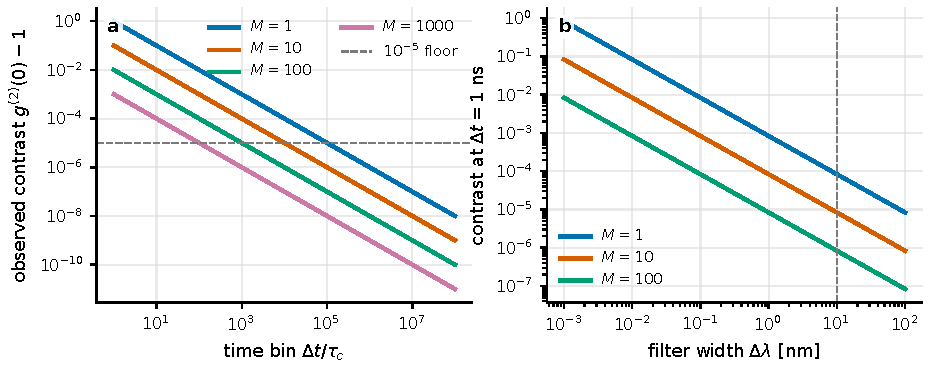
\includegraphics[width=0.96\linewidth]{figures/generated/chapter_21/ch21_g2_scaling_mistake.pdf}
\caption{时间箱、光谱带宽和模式数如何把 \(g^{(2)}\) 的对比度稀释。左图显示 \(\Delta t/\tau_c\) 和 \(M_{\rm eff}\) 怎样把单模热光的聚束峰一路压低；虚线标出 \(10^{-5}\) 量级的系统误差地板。右图把滤光片带宽换算成相干时间：在 \(1\,{\rm ns}\) 采样下，宽带可见光的热光峰很容易低到可校准范围之下。这正是"\(g^{(2)}\simeq1\)"的真实来历——不是没有量子性，而是量子性被平均稀释了。}
\label{fig:e27-g2-scaling}
\end{figure}

那么什么才是\textbf{真正过硬的非经典判据}？答案是反聚束（antibunching），即
\[
  g^{(2)}(0)<1.
\]
第 \ref{chap:e08} 章证明过：任何经典的随机强度都满足 \(g^{(2)}(0)\ge1\)（这是柯西–施瓦茨不等式的直接后果），所以 \(g^{(2)}(0)<1\) 是经典光\emph{无论如何也做不到}的事——它意味着光子彼此"回避"，是单量子发射体的标志。Kimble、Dagenais 和 Mandel 的共振荧光实验，就是靠测到 \(g^{(2)}(0)<1\) 才第一次坐实了反聚束 \citep{1977PhRvL..39..691K}。但要在天体光源里看到反聚束近乎不可能：天体的光通常是海量独立发射体、无数传播路径、有限探测器响应混在一起的结果，任何单个量子发射体的亚泊松特征，都会被式 \eqref{eq:e27-dilution} 里那个巨大的 \(M_{\rm eff}\) 稀释到看不见。

于是这一节的教训是双向的：一篇天文报告若写"\(g^{(2)}\simeq1\)，所以这是激光"，或写"\(g^{(2)}\simeq1\)，所以没有量子信息"，两句都没有依据。\(\mathbf{g^{(2)}\simeq1}\) \textbf{是被稀释后的默认结果，它既不证明相干、也不否证量子；只有 }\(\mathbf{g^{(2)}(0)<1}\)\textbf{ 才是不可辩驳的非经典证据。}


\section{强度干涉为什么依然离不开校准}
\label{sec:e27-calibration}

第三个坑源于对强度干涉一个真实优点的过度乐观。第 \ref{chap:e10} 章讲过，强度干涉（intensity interferometry）测的是两路强度涨落的相关，对大气整体相位（piston，即两路光程共同的平移相位）不敏感——这是它相对振幅干涉最大的工程优势，也是 Hanbury Brown 和 Twiss 当年能在 Narrabri 用简陋镜面测出恒星角直径的原因 \citep{1956Natur.178.1046H,1957RSPSA.242..300B,1974iiia.book.....H}。可"不怕相位"很容易被误读成"不怕误差"。事实恰恰相反：因为要找的信号已经被稀释到 \(10^{-5}\) 量级（上一节），任何一个同样量级的\emph{幅度}误差都能把结论掀翻。

把实际测到的相关超额写成一个数据模型，就能看清有哪些项在捣乱：

\begin{equation}
  \hat c_b(\tau)=
  \beta_b\,|V_b|^2\,h_b(\tau)
  +c_{{\rm inst},b}(\tau)
  +c_{{\rm sel},b}(\tau)
  +\epsilon_b(\tau).
  \label{eq:e27-calibration-model}
\end{equation}
\begin{formulaexplain}
\(\hat c_b=\hat g_b^{(2)}-1\) 是基线 \(b\) 上测到的归一化相关超额。第一项是真正的天体信号，后面依次是仪器项、选择项、随机误差。强度干涉不怕大气\emph{相位}，却照样怕这些\emph{幅度}项。
\end{formulaexplain}

逐项拆开，所有量都是无量纲的相关幅度。\(\hat c_b\) 是基线 \(b\)（一对望远镜、一段延迟）测到的归一化超额；\(\beta_b\) 是零基线对比度或仪器稀释因子，正是式 \eqref{eq:e27-dilution} 里那个 \(1/M_{\rm eff}\) 的具体体现；\(|V_b|^2\) 是天体可见度（visibility）的平方，携带角尺度信息；\(h_b(\tau)\) 是归一化的峰形。真正的麻烦在后三项：\(c_{\rm inst}\) 是电子学与探测器带来的伪相关——电子串扰、光电倍增管增益漂移、SPAD 死时间（dead time）、TDC 时间数字转换的量化伪峰；\(c_{\rm sel}\) 是选择函数、天气、背景处理造成的项；\(\epsilon\) 是随机噪声。VERITAS 在拟合恒星角直径时会显式处理背景光和零基线相关，MAGIC 的实时相关器则围绕连续记录、低串扰和快速模式切换设计 \citep{2020NatAs...4.1164A,2024MNRAS.529.4387A,2024ApJ...966...28A}。

这里有一个特别要命的误区：\textbf{以为只要积分够久，系统误差就会被压下去}。不会。随机误差 \(\epsilon\) 确实按 \(T^{-1/2}\) 随积分时间 \(T\) 缩小——积分一万倍时间，随机误差降一百倍。但式 \eqref{eq:e27-calibration-model} 里的 \(c_{\rm inst}\) 和 \(c_{\rm sel}\) 是\emph{系统}项，它们不随 \(T\) 衰减，只会形成一道"系统误差地板"（systematic floor）。一旦随机误差降到地板高度（对当前实验通常是 \(10^{-5}\)--\(3\times10^{-5}\)），继续积分就不再改善结论——曲线会\emph{饱和}。图 \ref{fig:e27-calibration} 左边画出一个电子串扰峰能比 \(5\times10^{-5}\) 的天体聚束峰高出一个量级以上，右边画出积分曲线撞上地板后的饱和。

\begin{figure}[tbp]
\centering
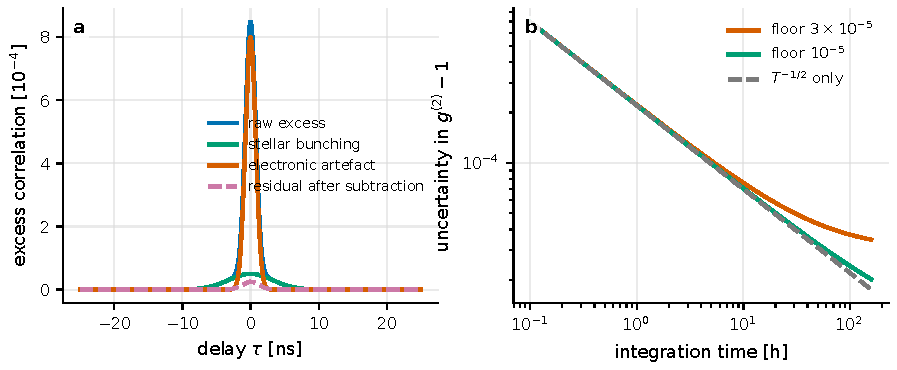
\includegraphics[width=0.96\linewidth]{figures/generated/chapter_21/ch21_calibration_artifacts.pdf}
\caption{校准误差如何伪装成相关信号。左图里电子串扰峰比 \(5\times10^{-5}\) 的天体聚束峰高出一个量级以上；若模板扣除后还留下窄残差，就会污染 \(\hat g^{(2)}(0)\)。右图显示积分时间只把\emph{统计}误差按 \(T^{-1/2}\) 压低；一旦存在 \(10^{-5}\)--\(3\times10^{-5}\) 的系统地板，再积分也不能自动改善结论。}
\label{fig:e27-calibration}
\end{figure}

对付系统项的正确姿势不是"积得更久"，而是设计一整套零检验（null test），让"真信号"和"伪信号"在不同操作下表现不同：时间平移（time-shift）把一路事件整体挪动远大于相关宽度的时间，真正的天体峰应当消失，慢漂移和背景结构则应保留；离源（off-source）或离带（off-band）把视场或频段换到不含目标的地方，零延迟峰不应保留；通道置换把本不该相关的探测器、偏振或谱通道交叉相关，若仍有峰，优先怀疑串扰；分块收敛把数据切成多段，相关幅度的均值应稳定，误差应按 \(T^{-1/2}\) 下降\emph{直到}撞上地板。Guerin 的报告指出，TDC 伪相关若不扣除会让信噪比提前饱和；AQuEye/IquEye 文献也明确列出 SPAD 死时间、光纤延迟、环境控制对系统误差的贡献 \citep{2017MNRAS.472.4126G,2016SPIE.9907E..0NZ,1996ApOpt..35.1956C,2013NIMPA.725..187J,2020RScI...91a3108W}。

收束：\textbf{强度干涉免掉的是大气相位，不是校准；信号既然被稀释到 }\(\mathbf{10^{-5}}\)\textbf{，就必须假设同量级的仪器伪相关一直在场，用零检验而不是用更长积分去对付它。}


\section{"没有相位"为什么不等于"不能成像"}
\label{sec:e27-phase}

第四个坑来自一句听上去很有道理的话："强度干涉丢了相位，所以只能测直径，不能成像。"前半句对，后半句错。

先把对的部分说清楚。第 \ref{chap:e10} 章的 van Cittert--Zernike 定理告诉我们，天体亮度分布 \(I(\boldsymbol\theta)\) 的角傅里叶变换就是复可见度 \(V(u,v)\)——它既有模又有相位。振幅干涉直接测这个复数 \(V\)；而强度干涉测的是两路强度相关，拿到的是模平方 \(|V(u,v)|^2\)，\textbf{一阶复可见度的相位确实丢掉了}。这是真实的信息损失，不能装作没有。

但"丢了相位"绝不等于"什么结构都测不出"。\(|V|^2\) 里仍然含着大量信息：均匀圆盘的直径、边缘昏暗（limb darkening）的程度、双星的间距与亮度比、旋转扁星的椭率、简单盘面的尺度，全都可以直接用 \(|V|^2\) 对 \(u,v\) 的依赖去拟合出来。第 \ref{chap:e11} 章讲从可见度到成像时，做的就是这件事。丢相位真正带来的困难，是一类特定的\textbf{退化}（degeneracy），其中最干净的一个是镜像退化。

镜像退化的道理，一行代数就能说透。设想把亮度分布整体做点对称反演，\(I(\boldsymbol\theta)\to I(-\boldsymbol\theta)\)。傅里叶变换有一条基本性质：函数做点对称反演，其频谱取复共轭。记原亮度 \(I(\boldsymbol\theta)\) 的复可见度为 \(V(\boldsymbol u)\)（即 \(V=\widetilde I\)），那么反演后的亮度 \(I(-\boldsymbol\theta)\) 其可见度为
\[
  \mathcal V_{I(-\boldsymbol\theta)}(\boldsymbol u)
  \equiv\widetilde{I(-\boldsymbol\theta)}(\boldsymbol u)
  =V^\ast(\boldsymbol u).
\]
于是取模平方，
\[
  \big|\mathcal V_{I(-\boldsymbol\theta)}(\boldsymbol u)\big|^2
  =\big|V^\ast(\boldsymbol u)\big|^2=\big|V(\boldsymbol u)\big|^2.
\]
两者\emph{完全相同}。这意味着：一个天体和它的镜像，产生的 \(|V|^2\) 一模一样，强度干涉\emph{原理上}就无法把它们分开——分开二者所需的方向信息，恰好藏在被丢掉的可见度相位符号里。第 \ref{chap:e11} 章已经画过这个相位缺失问题，图 \ref{fig:e27-phase-loss} 用一个不等亮双源和它的镜像再演示一次。

\begin{figure}[tbp]
\centering
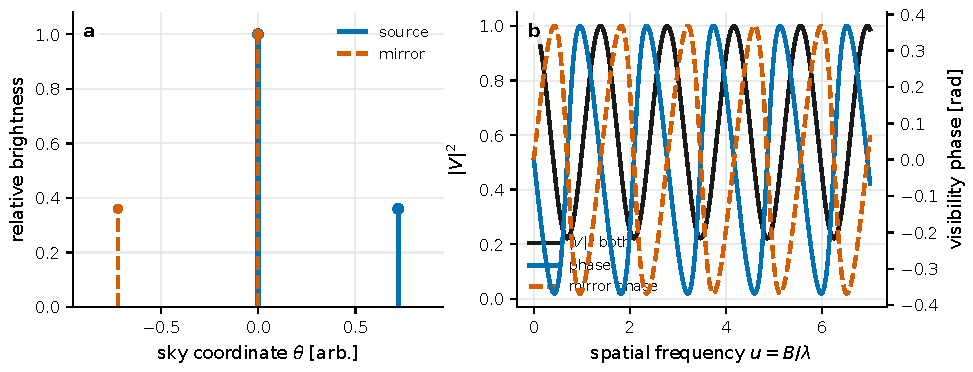
\includegraphics[width=0.96\linewidth]{figures/generated/chapter_21/ch21_phase_loss.pdf}
\caption{只测 \(|V|^2\) 带来的镜像退化。左图是一个不等亮双源和它的点对称镜像；右图显示二者的 \(|V|^2\) 完全重合，差别只在可见度相位的符号。强度干涉能约束结构，但要补回丢失的方向信息，得靠多基线覆盖、模型先验或高阶相关。}
\label{fig:e27-phase-loss}
\end{figure}

要把镜像、非对称结构、复杂形态区分开，正确的做法不是抱怨"没相位"，而是补信息：铺开多基线、加物理先验、用带正则化的相位反演（phase retrieval），或者引入三阶强度相关等高阶信息 \citep{2003RPPh...66..789M,2009A&A...507.1719F,2012NewAR..56..143D,2014MNRAS.437..798M,2022MNRAS.512.1722K}。其中三阶相关值得单说一句，因为它常被过度承诺：理想情况下，三阶强度相关能给出类似闭合相位（closure phase）的信息，从而部分补回方向；但它的信号比二阶相关\emph{更弱}。如果二阶相关的统计误差已经贴着上一节的系统地板，三阶相关会被同一批光子率和同一套校准问题卡得更死。所以三阶相关是大型阵列、极亮目标的探索方向，而第一代科学案例（第 \ref{chap:e25} 章）通常更务实——先从 \(|V|^2\) 的少参数模型做起，再逐步加先验做成像。

收束：\textbf{强度干涉丢的是可见度\emph{相位}，不是全部结构；}\(\mathbf{|V|^2}\)\textbf{ 足以约束直径、双星、扁率等许多量，真正丢掉的是区分镜像的方向信息，要靠多基线、先验或高阶相关补回。}


\section{量子超分辨为什么不能随意突破衍射}
\label{sec:e27-superres}

第五个坑，恰好长在一项真实成果的旁边，所以格外容易掉进去。SPADE（spatial-mode demultiplexing，空间模式解复用）纠正的是一个货真价实的统计误解：\textbf{Rayleigh 判据并不是所有参数估计问题的信息极限}。第 \ref{chap:e12} 章一步不跳地证明过：对两个弱、等亮、互不相干的点源，当角间距 \(s\) 远小于点扩散函数宽度 \(\sigma\) 时，直接成像对 \(s\) 的 Fisher 信息（Fisher information）以 \(s^2\) 的速度掉到零（这就是所谓的"Rayleigh 诅咒"），而理想的空间模式排序能把每光子的 Fisher 信息保持在有限值 \citep{2015Optic...2..646T,2016PhRvX...6c1033T,2016OExpr..24.3684N,2017PhRvL.118g0801T}。这是真结论，别打折。

但恰恰因为它是真的，才更要防止被夸张成"量子超分辨能任意突破衍射、能从几个光子里重建任意复杂图像"。要看清边界，回到第 \ref{chap:e12} 章的 Cramér--Rao 下界（Cramér--Rao bound）。任何无偏估计量 \(\hat s\) 的方差满足
\begin{equation}
  \operatorname{Var}(\hat s)\;\ge\;\frac{1}{N_\gamma\,F_s},
  \label{eq:e27-crb}
\end{equation}
\begin{formulaexplain}
\(\hat s\) 是对角间距的估计，\(N_\gamma\) 是进入正确模式分析的光子数，\(F_s\) 是\emph{每个光子}对 \(s\) 的 Fisher 信息。测量方式只能改 \(F_s\)，改不了 \(N_\gamma\)；下界要真达到，还得没有背景、像差和模式串扰。
\end{formulaexplain}

逐符号落实。\(s\) 是待估的角间距，单位可用 rad、mas，或直接以 PSF 宽度 \(\sigma\) 归一化；\(N_\gamma\) 是无量纲的有效光子数——注意是\emph{进入了正确模式分析}的光子数，不是打到望远镜上的总光子数；\(F_s\) 是每光子 Fisher 信息，量纲是角度的 \(-2\) 次方。式 \eqref{eq:e27-crb} 把三件事一次讲明白：第一，SPADE 提高的是 \(F_s\)（把 \(s^2\to0\) 的坍塌堵住），它\textbf{替代不了 }\(N_\gamma\)——光子数太少，方差照样爆炸；第二，下界是"\(\ge\)"，是可能达到的\emph{最好}情形，\textbf{量子下界不会自动可达}，背景、像差、模式串扰、质心（centroid）误差每一样都会让实际方差高于这条线；第三，把两点源的结论套到任意复杂图像上是没有根据的。图 \ref{fig:e27-superresolution} 左边画出模式排序确实把误差标度大幅拉低，但一道 \(0.003\sigma\)--\(0.01\sigma\) 的模式/质心误差地板会终止改善；右边用一个玩具模型显示，想恢复更高阶的矩或模式，所需光子数会\emph{急剧}上升。

\begin{figure}[tbp]
\centering
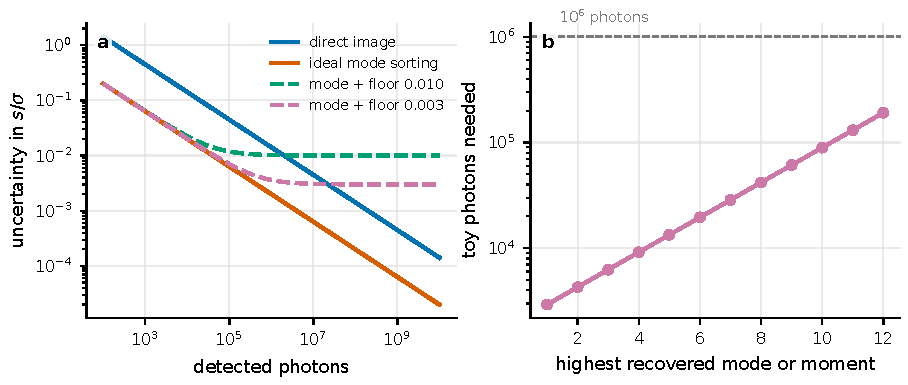
\includegraphics[width=0.96\linewidth]{figures/generated/chapter_21/ch21_superresolution_budget.pdf}
\caption{量子超分辨的光子预算与系统地板。左图取 \(s=0.2\sigma\)，比较直接成像与理想模式排序的统计误差标度：模式排序显著降低误差，但 \(0.003\sigma\)--\(0.01\sigma\) 的模式/质心误差地板会让改善停下来。右图用玩具模型显示，恢复更高阶矩或模式所需的光子数快速上升——复杂图像不可能从少数光子里任意恢复。}
\label{fig:e27-superresolution}
\end{figure}

天文语境里还有一层更细的条件常被忽略：源本身的相干性，以及传播之后的一阶空间相干。SPADE 的干净结论是对"两点\emph{互不相干}高斯源"证的；一旦源是部分相干（partially coherent）的，模式概率会改变，Rayleigh 诅咒是否重新出现，学界的讨论正是围绕这个条件展开 \citep{2017NJPh...19b3054T,2017PhRvA..95f3847A,2018Optic...5.1177P,2018Optic...5.1382L,2019Optic...6..400T}。因此，把"两点非相干高斯源"的结论直接搬到星系、吸积盘、喷流或强透镜弧上，会悄悄丢掉适用条件。

收束：\textbf{Rayleigh 判据不是估计极限，这是 SPADE 的真本事；但式 }\eqref{eq:e27-crb}\textbf{ 里的量子下界既需要足够的 }\(\mathbf{N_\gamma}\)\textbf{、又不会自动可达，脱离"两点、非相干、无背景、模式对齐"这些条件，超分辨就只剩一个口号。}


\section{天体 laser、maser 与非泊松统计最容易混在哪里}
\label{sec:e27-maser}

第六个坑集中在天体受激辐射源上，而且是好几条误会拧在一起。最典型的一句是："天体 laser/maser 一定给 \(g^{(2)}=1\)。"

先拆第一层：\textbf{高亮温（high brightness temperature）不等于相干态}。受激辐射能产生极高的亮温、极窄的谱线、很强的偏振——这些是 maser（microwave amplification by stimulated emission，微波受激辐射放大）的招牌。但招牌不等于内在统计。实验室激光之所以逼近相干态，靠的是稳定的谐振腔加饱和增益把强度涨落钳住；天体环境里根本没有这样的腔。第 \ref{chap:e06} 章分清过：相干态是一个很特殊的量子态，它的指纹是\emph{泊松}光子数分布，而不是"亮"或"窄"。一条谱线又亮又窄，完全可能仍带着很强的强度涨落——亮温、线宽、偏振是"多亮多窄多整齐"的度量，光子统计是"涨落多大"的度量，两把尺子量的是不同的东西。未饱和 maser、饱和 maser、速度相干路径、泵浦（pump）涨落、多个斑点叠加、连续谱背景，每一样都会改写光子统计 \citep{1982RvMP...54.1225E,1992ARA&A..30...75E,1985ARA&A..23..169D}。Eta Carinae 的 Weigelt blobs 里，Fe II 和 O I 线的自然激光候选，就要同时看 Ly\(\alpha\) 泵浦、能级反转、线宽、空间位置和连续谱扣除才能定性；Brown--Twiss--Townes 外差相关甚至被提出来专门去测那条极窄 Fe II 线的线宽 \citep{2004A&A...428..497J,2005MNRAS.364..731J,2005NewA...10..361J,2008AIPC..984..216D}。

第二层是混合稀释，值得把公式一步不跳地推出来。设观测到的光由若干独立成分叠加，总强度 \(I=\sum_a I_a\)，不同成分之间没有强度相关。零延迟的二阶相干是
\[
  g^{(2)}_{\rm mix}(0)=\frac{\langle I^2\rangle}{\langle I\rangle^2}.
\]
先算分子。展开 \(I^2=\big(\sum_a I_a\big)^2=\sum_a I_a^2+\sum_{a\ne b}I_aI_b\)，取平均：
\[
  \langle I^2\rangle
  =\sum_a\langle I_a^2\rangle
  +\sum_{a\ne b}\langle I_a\rangle\langle I_b\rangle,
\]
其中交叉项用了"不同成分无相关"这条假设，把 \(\langle I_aI_b\rangle\) 拆成 \(\langle I_a\rangle\langle I_b\rangle\)。再用每个成分自己的定义 \(\langle I_a^2\rangle=g_a^{(2)}(0)\langle I_a\rangle^2\)，并把交叉求和补全成完整双重求和再减去对角：
\[
  \sum_{a\ne b}\langle I_a\rangle\langle I_b\rangle
  =\Big(\sum_a\langle I_a\rangle\Big)^2-\sum_a\langle I_a\rangle^2
  =\langle I\rangle^2-\sum_a\langle I_a\rangle^2.
\]
合起来：
\[
  \langle I^2\rangle
  =\sum_a g_a^{(2)}(0)\langle I_a\rangle^2
  +\langle I\rangle^2-\sum_a\langle I_a\rangle^2.
\]
两边除以 \(\langle I\rangle^2\)，并记通量分数 \(f_a=\langle I_a\rangle/\langle I\rangle\)：
\[
  g^{(2)}_{\rm mix}(0)
  =\sum_a g_a^{(2)}(0)f_a^2+1-\sum_a f_a^2.
\]
把 1 挪到左边，右边按 \(f_a^2\) 合并，得到干净的结果：

\begin{equation}
  g^{(2)}_{\rm mix}(0)-1
  =\sum_a f_a^2\left[g_a^{(2)}(0)-1\right],
  \qquad
  f_a=\frac{\langle I_a\rangle}{\sum_b\langle I_b\rangle}.
  \label{eq:e27-mixture}
\end{equation}
\begin{formulaexplain}
\(f_a\) 是第 \(a\) 个成分的通量分数（无量纲，各成分之和为 1）。关键在那个\emph{平方}：相关超额按 \(f_a^2\) 加权，所以一点点热连续谱或多成分混合，就能把 \(g^{(2)}\) 的解读搅乱。
\end{formulaexplain}

那个平方是全部要害。代个数字：一个只占总通量 \(20\%\) 的热成分，即使它自己满格 \(g_a^{(2)}(0)-1=1\)，混进来后也只贡献 \(f_a^2\times1=0.2^2=0.04\) 的对比度；若这个热成分再摊到 \(M=100\) 个模式、\(\tau_c/\Delta t=10^{-5}\)，观测对比度就成了 \(0.04\times10^{-5}/100\sim4\times10^{-9}\)——彻底沉底。反过来，一条未饱和的受激线若带着泵浦强度噪声，可能给出\emph{超}泊松（super-Poisson）统计；但这种结果得先把谱线、连续谱、仪器响应分离干净，绝不能一见 \(g^{(2)}>1\) 就归给新物理。图 \ref{fig:e27-maser} 把这两条分支画在一起。

\begin{figure}[tbp]
\centering
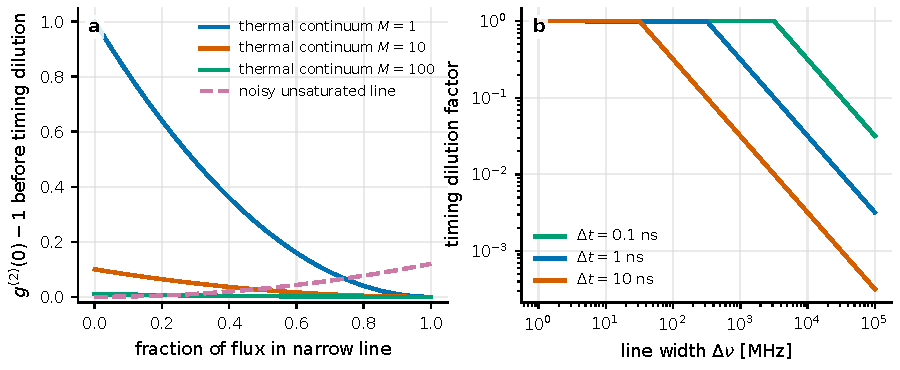
\includegraphics[width=0.96\linewidth]{figures/generated/chapter_21/ch21_maser_mixed_statistics.pdf}
\caption{天体 maser/laser 候选中的混合统计。左图显示窄线通量分数增大时，热连续谱的聚束按 \(f_a^2\) 被稀释；若窄线本身带未饱和强度噪声，则冒出另一条超泊松分支。右图显示谱线宽度和电子学时间箱对相关对比度的稀释——MHz--GHz 的线宽需要 ns 甚至更快的时间响应，才能保住可观的峰值。}
\label{fig:e27-maser}
\end{figure}

第三层：非泊松统计有太多\emph{普通}来源，别急着往量子光源上想。最典型的是把随机变源当成 Cox 过程（Cox process，又称双随机泊松过程）：给定瞬时率 \(\Lambda\) 时计数服从泊松，但 \(\Lambda\) 自己随时间或环境涨落。用全方差公式（law of total variance，把方差拆成"条件方差的期望"加"条件期望的方差"）算一算，记 \(\Lambda\) 为一个箱里的期望计数，泊松条件下 \(\operatorname{Var}(N\mid\Lambda)=\Lambda\)、\(\mathbb E(N\mid\Lambda)=\Lambda\)，于是
\[
  \operatorname{Var}(N)
  =\mathbb E[\operatorname{Var}(N\mid\Lambda)]+\operatorname{Var}(\mathbb E[N\mid\Lambda])
  =\mathbb E(\Lambda)+\operatorname{Var}(\Lambda),
\]
而 \(\mathbb E(N)=\mathbb E(\Lambda)\)。两者相除即得 Fano 因子（Fano factor）：

\begin{equation}
  F_{\rm Fano}
  \equiv\frac{\operatorname{Var}(N)}{\mathbb E(N)}
  =1+\frac{\operatorname{Var}(\Lambda)}{\mathbb E(\Lambda)}.
  \label{eq:e27-fano}
\end{equation}
\begin{formulaexplain}
\(F_{\rm Fano}\) 是计数方差与均值之比（纯泊松等于 1）。只要瞬时率 \(\Lambda\) 自己在涨落，计数就自然变成超泊松（\(F>1\)），根本不必先请出非经典光源。
\end{formulaexplain}

也就是说，只要源在变，\(F_{\rm Fano}\) 在合适的箱宽下就\emph{必然}大于 1，这是最平凡的超泊松。仪器还会从反方向捣乱：死时间会压掉挨得太近的事件，让短延迟出现负相关、把 \(F_{\rm Fano}\) 压到 1 以下（欠离散，under-dispersion）；afterpulsing（余脉冲）则会在探测器特征时间之后制造正相关。第 \ref{chap:e07} 章给过的 afterpulsing 概率 \(10^{-4}\)--\(10^{-2}\)，已经足以污染许多短延迟搜索。所以在喊"非泊松"之前，先把这几张诊断图画全：Fano 因子随箱宽的变化、短延迟自相关与互相关、暗场数据、离源数据、时间平移背景。图 \ref{fig:e27-nonpoisson} 把这些普通来源的不同标度并排画了出来。

\begin{figure}[tbp]
\centering
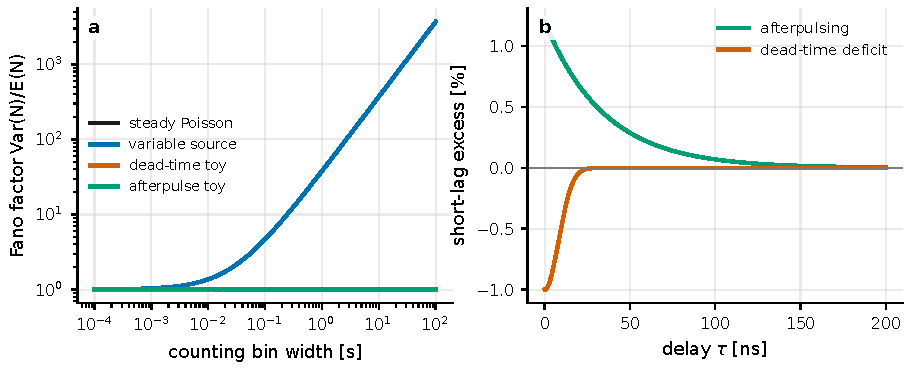
\includegraphics[width=0.96\linewidth]{figures/generated/chapter_21/ch21_nonpoisson_diagnostics.pdf}
\caption{非泊松统计的普通来源。左图用 Fano 因子展示稳态泊松、慢变源、死时间和 afterpulsing 各自不同的标度：慢变源在长箱里变成超泊松，死时间造成欠离散。右图显示 afterpulsing 与死时间在短延迟相关函数里的相反形状——这些仪器特征应先从暗场和交叉通道里量化出来。}
\label{fig:e27-nonpoisson}
\end{figure}

收束：\textbf{亮、窄、偏振强都不等于相干态；混合光按 }\(\mathbf{f_a^2}\)\textbf{ 稀释相关，变源与死时间、余脉冲会自然造出非泊松统计——把它们排除干净之前，任何"非泊松"都不该记在新物理头上。}


\section{假警报如何伪造出"新物理"的边界}
\label{sec:e27-false-alarm}

最后一个坑，是所有搜索类工作的通病：把一次小概率事件当成发现。

问题的根子是"多重检验"（multiple testing）。设一次检验偶然给出如此极端结果的尾概率是 \(p_0\)，而你独立地做了 \(N_{\rm trial}\) 次检验，那么"至少出现一次"这种偶然峰的概率是多少？逐步算：单次\emph{不}出现的概率是 \(1-p_0\)，\(N_{\rm trial}\) 次全都不出现是 \((1-p_0)^{N_{\rm trial}}\)（用了各次独立），于是至少出现一次是

\begin{equation}
  p_{\rm any}=1-(1-p_0)^{N_{\rm trial}}
  \simeq N_{\rm trial}\,p_0
  \qquad(N_{\rm trial}\,p_0\ll1).
  \label{eq:e27-trials}
\end{equation}
\begin{formulaexplain}
\(p_0\) 是单次检验的尾概率，\(N_{\rm trial}\) 是试验次数。搜索空间越大，偶然撞见一次高峰的概率越高，所以要报告\emph{全局}显著性，而不是单次的 \(p_0\)。
\end{formulaexplain}

那个约等号来自一步标准展开：当 \(p_0\) 很小、\emph{且} \(N_{\rm trial}p_0\ll1\) 时，\((1-p_0)^{N_{\rm trial}}\approx e^{-N_{\rm trial}p_0}\approx1-N_{\rm trial}p_0\)（先用 \(\ln(1-p_0)\approx-p_0\)，再对指数做一阶泰勒展开），代回即得 \(p_{\rm any}\approx N_{\rm trial}p_0\)。务必记住这条近似\textbf{只在 }\(\mathbf{N_{\rm trial}p_0\ll1}\)\textbf{ 时成立}；一旦搜索空间大到 \(N_{\rm trial}p_0\gtrsim1\)，就不能再用它，得回到未近似的 \(p_{\rm any}=1-(1-p_0)^{N_{\rm trial}}\approx1-e^{-\mu}\)，其中我们记
\[
  \mu\equiv N_{\rm trial}\,p_0
\]
为偶然峰的\textbf{期望个数}（无量纲，可以远大于 1），而概率 \(p_{\rm any}=1-e^{-\mu}\) 始终落在 \(0\) 与 \(1\) 之间。这个 \(N_{\rm trial}\) 可以从四面八方冒出来：时间箱数、频率通道数、基线数、目标数、模型网格点数，甚至事后才圈定的窗口。代个数字体会一下：若每晚扫描 \(10^6\) 个候选的延迟/频率/目标组合，一个单次 \(p_0=10^{-5}\)（听起来已经"很显著"）的事件，其偶然峰的期望个数是
\[
  \mu=N_{\rm trial}\,p_0\simeq10^{6}\times10^{-5}=10,
\]
于是全局出现的概率是
\[
  p_{\rm any}=1-e^{-\mu}\approx1-e^{-10}\approx0.99995\approx1,
\]
几乎必然——意思是每晚平均约有 \(\mu\approx10\) 个这样的"惊人峰"冒出来，纯属搜索空间的自然尾部。这里要特别把两件事分清：\(10\) 是期望\emph{个数} \(\mu\)，不是概率；把它写成 \(p_{\rm any}=10\)（并顺手把只在 \(\mu\ll1\) 时成立的近似式 \(p_{\rm any}\approx N_{\rm trial}p_0\) 硬套到 \(\mu=10\) 上）正是本节要教你避开的典型错误——概率永远不会超过 1，超过 1 的那个量一定是计数的期望值。图 \ref{fig:e27-false-alarm} 左边画出 \(\mu=8\) 的单个泊松箱偶尔会甩出 \(N\ge17\) 的高计数尾，右边画出同一个单次 \(p_0\) 在大量试验后如何滚成很高的全局假警报概率。

\begin{figure}[tbp]
\centering
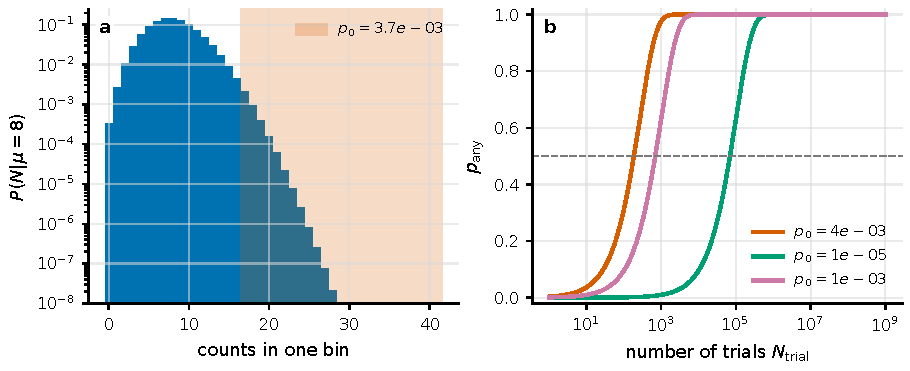
\includegraphics[width=0.96\linewidth]{figures/generated/chapter_21/ch21_poisson_false_alarm.pdf}
\caption{泊松尾部与多重检验。左图里 \(\mu=8\) 的单个箱偶尔会出现 \(N\ge17\) 的高计数尾；右图显示同样的单次 \(p_0\) 在大量试验中如何变成很高的全局假警报概率。事件表搜索、周期搜索、跨频相关、暂现源筛选，都必须报告 \(N_{\rm trial}\) 或等效的全局显著性。}
\label{fig:e27-false-alarm}
\end{figure}

顺带纠正一个更大的语义误会：\textbf{"量子天文学"不等于"量子引力"}。本书前面绝大部分内容研究的是光场统计、模式测量、相干函数、仪器和信息极限——都是可测的地面物理。黑洞、CMB、轴子、宇宙双折射、暗物质透镜之所以能进这条主线，是因为它们能被写成\emph{可观测}的时间、频率、偏振或空间相关量，而不是因为每个话题都得动用普朗克尺度物理。一个真正可检查的异常，第一步永远是把数据来源拆开：
\begin{equation}
  d_{\rm obs}=d_{\rm sky}(\boldsymbol\theta)
  +d_{\rm inst}(\boldsymbol\phi)
  +d_{\rm sel}(\boldsymbol\psi)
  +n.
  \label{eq:e27-data-model}
\end{equation}
\begin{formulaexplain}
\(d_{\rm obs}\) 是观测数据（延迟直方图、\(|V|^2\)、偏振相关或事件时间）；右边把天空模型、仪器模型、选择函数和噪声分开。任何"新物理"解释都得先证明前面这些普通项\emph{解释不了}数据。
\end{formulaexplain}

其中 \(d_{\rm sky}(\boldsymbol\theta)\) 是天体模型（参数 \(\boldsymbol\theta\)），\(d_{\rm inst}(\boldsymbol\phi)\) 是仪器模型，\(d_{\rm sel}(\boldsymbol\psi)\) 是选择函数，\(n\) 是噪声。只要这四项还没分开，异常峰、偏振旋转或超泊松计数就都不该直接归因于新物理——它们更可能藏在 \(d_{\rm inst}\) 或 \(d_{\rm sel}\) 里。这也正好接上第 \ref{chap:e28} 章：一份研究计划的最后一页，应当回到"新增的观测量到底是什么"——是平均强度、二阶相关、跨频协方差、偏振相关，还是模式计数；每个量都要配上单位、典型范围、适用条件（热光、高斯 PSF、弱光、少参数源模型、稳定仪器响应），并至少从时间平移、离源、离带、暗场、错偏振、注入恢复里挑两个零检验，把全局显著性和系统误差地板\emph{一起}写进结论。

收束：\textbf{搜索空间越大，偶然的"显著峰"越是必然；不报告 }\(\mathbf{N_{\rm trial}}\)\textbf{ 的显著性没有意义，而"量子天文学"的门槛是可观测的相关量，不是普朗克尺度的新物理。}


\section{本章要点}
\label{sec:e27-summary}

\begin{itemize}
  \item \textbf{数光子只是拿到原料。}真正的量子信息在事件之间的联合分布里；若时间、探测器、频率、偏振标签不进模型，再精密的单光子计数也还是经典测光。"少光子"与"量子"是两把尺子。
  \item \(\mathbf{g^{(2)}\simeq1}\)\textbf{ 什么也证明不了。}热光的聚束峰被有效模式数 \(M_{\rm eff}\)（含 \(\Delta t_{\rm eff}/\tau_c\)）稀释到 \(10^{-5}\)--\(10^{-6}\) 是常态，见式 \eqref{eq:e27-dilution}。唯一过硬的非经典判据是反聚束 \(g^{(2)}(0)<1\)，经典光做不到。
  \item \textbf{强度干涉不怕相位，但怕校准。}信号既已稀释到 \(10^{-5}\)，就得假设同量级的仪器伪相关一直在场（式 \eqref{eq:e27-calibration-model}）。系统地板不随 \(T^{-1/2}\) 下降，靠零检验而非更长积分来对付。
  \item \(\mathbf{|V|^2}\)\textbf{ 丢的是相位，不是结构。}直径、双星、扁率都能拟合，真正丢的是区分镜像的方向信息（\(|V^\ast|^2=|V|^2\)），要靠多基线、先验或高阶相关补回。
  \item \textbf{量子超分辨有边界。}Rayleigh 判据确实不是估计极限，但式 \eqref{eq:e27-crb} 的量子下界既要足够光子 \(N_\gamma\)、又不会自动可达；离开"两点、非相干、无背景、模式对齐"就只剩口号。
  \item \textbf{亮窄偏振强不等于相干态。}混合光按 \(f_a^2\) 稀释相关（式 \eqref{eq:e27-mixture}），变源（Cox 过程，式 \eqref{eq:e27-fano}）、死时间、余脉冲都会自然造出非泊松统计——排除干净前不算新物理。
  \item \textbf{搜索必报全局显著性。}偶然峰随 \(N_{\rm trial}\) 线性增多（式 \eqref{eq:e27-trials}）；异常要先按天空/仪器/选择/噪声四项拆开（式 \eqref{eq:e27-data-model}），才谈得上新物理。
\end{itemize}

\medskip
\noindent\textbf{想一想。}
\begin{itemize}
  \item 你在 \(500\,{\rm nm}\)、\(5\,{\rm nm}\) 带宽下用 \(2\,{\rm ns}\) 的相关箱测一颗恒星的热光。单模情形下，你预期测到的 \(g^{(2)}_{\rm meas}(0)-1\) 大概是什么量级？（提示：先算 \(\tau_c\)，再用式 \eqref{eq:e27-dilution}。）
  \item 一次谱线搜索里，你在 \(3\times10^{5}\) 个频率通道中找到一个单次 \(p_0=3\times10^{-6}\) 的峰。它的全局假警报概率是多少？你会宣布发现吗？
  \item 有人报告某天体 maser 的 \(g^{(2)}(0)=1.5\)，声称是非经典光。在相信之前，你会先要求他排除哪三种普通来源？
\end{itemize}

\chapter{从白皮书到研究计划}
\label{chap:e28}

\begin{chapteropening}
到这里，整本书的工具箱已经装满：复振幅与相位（第 \ref{chap:e01} 章）、带宽与相干时间（第 \ref{chap:e02} 章）、泊松与散粒噪声（第 \ref{chap:e03} 章）、二阶相干 \(g^{(2)}\) 与 Siegert 关系（第 \ref{chap:e08} 章）、强度干涉与 van Cittert--Zernike 定理（第 \ref{chap:e10} 章）、从可见度到成像（第 \ref{chap:e11} 章）、量子估计与 SPADE（第 \ref{chap:e12} 章）、事件表与时钟（第 \ref{chap:e13} 章）、相关器（第 \ref{chap:e14} 章）、误差预算与可行性（第 \ref{chap:e15} 章）、再到把恒星、致密星、黑洞、瞬变当成量子光源（第 \ref{chap:e17}--\ref{chap:e20} 章）与第一代科学案例（第 \ref{chap:e25} 章）。工具齐了，本章要回答的却是一个不那么"物理"、却决定一切能否发生的问题：\textbf{怎样把一个漂亮的想法，写成一份真的能执行、也真的可能失败的研究计划？}我们会沿着一条清晰的路径走一遍——\textbf{提出科学问题 \(\to\) 选目标与方法 \(\to\) 写误差预算、估算可达精度 \(\to\) 规划仪器与数据流程 \(\to\) 排里程碑、登记风险 \(\to\) 写成计划}——每一步都把前面某一章的公式，落成 proposal 里一个可以被审查、被复现、被打分的条目。这一章的语气会稍微转向"你"的下一步行动：读完它，你应该能把一个念头改写成工作包、验收指标和失败判据。
\end{chapteropening}

\section{从科学问题出发：先选对目标，再谈仪器}
\label{sec:e28-question}

写计划最常见的失败，不是"仪器不够好"，而是\textbf{一开始就把顺序搞反了}——先爱上一台仪器或一个时髦词（"量子""纠缠""网络"），再去找题目。正确的次序永远是：先问一个能被观测证伪的\textbf{科学问题}，再问哪个\textbf{可观测量}（observable）能回答它，最后才问需要什么仪器、什么精度、什么样的目标源。

一个可执行的科学问题，通常长这样：不是"我想研究恒星"，而是"这颗快速自转星的赤道到底比两极暗多少、扁到什么程度"；不是"我想做量子天文学"，而是"这条自然激光候选线的光子统计，是热的还是相干的"。前者含糊、无法收敛；后者立刻指向一个可观测量（\(|V|^2\) 随位置角的变化、\(g^{(2)}(0)\) 偏离 1 的量），也立刻指向一套仪器需求。

选目标时，第 \ref{chap:e25} 章那三把尺子仍然管用：\textbf{亮度}决定"有没有光子"，\textbf{角尺度}决定"这些光子能不能变成参数"，\textbf{外部先验}决定"参数能不能被唯一地翻译成物理"。但写计划时还要多加一条尺子，它在纯科学讨论里常被忽略，在 proposal 里却是生死线——\textbf{失败后是否仍有产出}。一个好计划即使主目标没检出，也应留下可复用的东西：一套定标好的事件表格式、一版公开的相关器、一张校准星表、一组时间同步的 null test。把这条写进目标选择，你就不会把全部赌注押在一次可能落空的检出上。

这一步的产物很朴素，却是整份计划的地基：一句话的科学问题 + 一个明确的可观测量 + 一份"为什么是这个目标而不是那个"的排序理由。后面所有的误差预算、仪器设计、里程碑，都是在服务这一句话。第 \ref{chap:e27} 章列的那些常见误区（把多模热光当激光、把单方向基线当成能定形状、把可见度当成能直接读相位），很多都源于\textbf{在这一步偷懒}——没把"要测什么、能证伪什么"想透，就急着上仪器。

\section{近期能落地什么：把强度干涉做成常规数据产品}
\label{sec:e28-nearterm}

先说\textbf{现在就能做}的那一档。近期（可预见的这几年）最成熟、最该优先写成 proposal 的，是把已经被 VERITAS 和 MAGIC 反复验证过的强度干涉，从"一次演示"变成"可重复的数据产品" \citep{2020NatAs...4.1164A,2024MNRAS.529.4387A}。量子网络望远镜很迷人，但它属于后面的阶段（第 \ref{chap:e24} 章），近期不该占用第一批工作包。

这个阶段的主要可观测量是：二阶相干 \(\hat g^{(2)}_{ab}(\tau)\)、平方可见度 \(|V_{ab}|^2\)、每台望远镜的目标光子率、零基线对比度、背景稀释因子，以及每条基线上的协方差。问题是：怎样判断一个近期项目\textbf{到底成不成熟}？"探测器可用""望远镜够大"这种话不能写进 proposal，因为它们不可验收。我们需要一个能打分的成熟度判据。

把项目成熟度写成一个\textbf{比值向量}，每一项都是"实际能力 \(\div\) 需求"：
\begin{equation}
  \bm{r}=
  \left(
  \frac{R_\gamma}{R_{\rm req}},\;
  \frac{\sigma_{t,{\rm req}}}{\sigma_t},\;
  \frac{\beta_0}{\beta_{\rm req}},\;
  \frac{\sigma_{{\rm sys,req}}}{\sigma_{\rm sys}},\;
  \frac{N_{\rm cal}}{N_{{\rm cal,req}}}
  \right).
  \label{eq:e28-readiness}
\end{equation}
\begin{formulaexplain}
\(\bm r\) 是项目成熟度向量。每一项都是"实际能力比需求"：光子率、计时精度、零基线对比度、系统误差地板、校准样本。只有五项\textbf{同时}都 \(\ge1\)，近期项目才算闭合。任何一项 \(<1\)，都是必须先补的短板。
\end{formulaexplain}
逐个把符号、单位和量纲交代清楚，这是把 \eqref{eq:e28-readiness} 从"漂亮的向量"变成"可核账的清单"的关键。\(R_\gamma\) 是每台望远镜的有效目标光子率，单位 \(\mathrm{s^{-1}}\)，由集光面积、量子效率、滤光带宽和目标亮度共同决定；\(R_{\rm req}\) 是达到目标精度所需的光子率。\(\sigma_t\) 是望远镜之间的相对时间同步误差，单位常取 ps 或 ns；注意这一项是\textbf{需求比能力}（\(\sigma_{t,{\rm req}}/\sigma_t\)），因为误差越小越好，所以要让"需求"在分子。\(\beta_0\) 是零基线相关对比度（无量纲），衡量仪器在"两台望远镜看同一束光"时能恢复多大的相关信号；\(\beta_{\rm req}\) 是所需对比度。\(\sigma_{\rm sys}\) 是校准后残余的系统误差地板（无量纲，和 \(|V|^2\) 同单位），同样以"需求比能力"入列。\(N_{\rm cal}\) 是可用的校准星或校准观测数，\(N_{\rm cal,req}\) 是所需数目。

这个向量的价值在于它\textbf{防止单项掩盖短板}。举个反例：假设你的光子率极高，\(R_\gamma/R_{\rm req}=5\)，看起来很富裕；但如果系统误差地板 \(\sigma_{\rm sys}=3\times10^{-5}\) 却比你想测的 \(|V|^2\) 小信号还大，那么 \(\sigma_{\rm sys,req}/\sigma_{\rm sys}<1\)，项目照样不成熟——再多的光子也压不平一个系统性的偏差。强度干涉阵列的研究反复强调这一点：基线长度、\(u,v\) 覆盖、背景控制和零基线校准必须\textbf{一起}闭合，缺一不可 \citep{2006ApJ...649..399L,2013APh....43..331D,2022MNRAS.512.1722K}。

\begin{figure}[tbp]
\centering
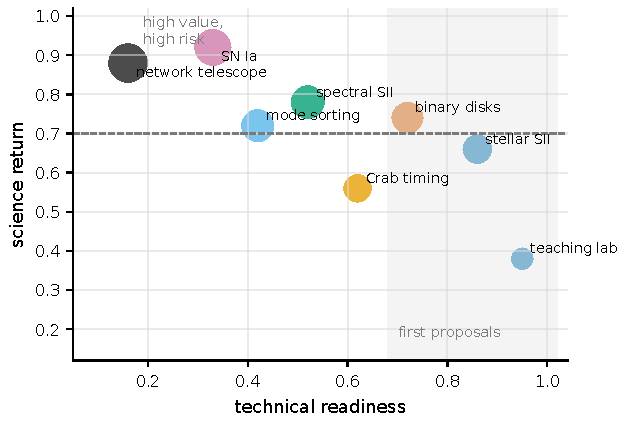
\includegraphics[width=0.86\linewidth]{figures/generated/chapter_22/ch22_roadmap_trade_space.pdf}
\caption{路线图中的技术成熟度、科学回报、成本与风险。横轴技术成熟度、纵轴科学回报，点越大表示成本压力越大。右上方且成熟度高的任务适合写成近期 proposal；左上方科学价值高但需要先做路径验证（pathfinder）的任务，属于中远期。这张图是式 \eqref{eq:e28-readiness} 那套"先看短板再谈价值"的可视化。}
\label{fig:e28-trade-space}
\end{figure}

写近期计划时，题目越具体越好。可执行的题目可以是"用四台 IACT 在 416 nm 附近测量 10--30 颗亮星的角直径，并公开相关器与校准库"，或"用同一套 pipeline 比较双星、Be 星盘和快速自转星的 \(|V|^2\) 模型"。每一篇论文都应发布：事件表格式说明、相关器版本号、time-shift null test、校准星表、基线几何、后验样本。这样即便部分目标没有检出，也留下了可复用的仪器知识——正是上一节说的"失败后仍有产出"。

\section{误差预算与可行性：先估出你能达到的精度}
\label{sec:e28-budget}

计划里最不能省、审稿人第一眼要看的，就是\textbf{误差预算}（error budget）——第 \ref{chap:e15} 章的核心工具。它回答两个问题："我这次观测最终能把可观测量测到多准？""是统计噪声、还是某个系统误差，卡住了这个精度？"没有误差预算的 proposal，等于说"我要去做，但不知道能做到多好"，几乎必被拒。

误差预算的骨架，是把各路独立误差按\textbf{平方相加}（add in quadrature）。为什么是平方相加而不是直接相加？因为若干个\textbf{互相独立}的随机误差，其总方差等于各自方差之和（这是概率论里独立随机变量方差可加的直接结果，第 \ref{chap:e03} 章讲过）。设各误差源的标准差为 \(\sigma_{\rm stat},\sigma_{\rm cal},\sigma_{\rm bg},\sigma_{\rm model},\sigma_{\rm sel}\)，则总误差为
\begin{equation}
  \sigma_{\rm tot}^2
  =
  \sigma_{\rm stat}^2
  +\sigma_{\rm cal}^2
  +\sigma_{\rm bg}^2
  +\sigma_{\rm model}^2
  +\sigma_{\rm sel}^2 .
  \label{eq:e28-error-budget}
\end{equation}
\begin{formulaexplain}
各项都是某一路误差对最终可观测量贡献的标准差（与可观测量同量纲）：\(\sigma_{\rm stat}\) 统计、\(\sigma_{\rm cal}\) 校准、\(\sigma_{\rm bg}\) 背景、\(\sigma_{\rm model}\) 模型、\(\sigma_{\rm sel}\) 选择效应。独立误差按方差相加，所以\textbf{最大的那一项主导总误差}——先去压它。
\end{formulaexplain}
逐项落地，也顺带说清各项从哪儿来。\(\sigma_{\rm stat}\) 是统计噪声，来自泊松或相关计数的有限样本，随积分时间按 \(T^{-1/2}\) 下降。\(\sigma_{\rm cal}\) 是校准误差，来自零基线对比度、时间同步、偏振与光谱响应的不完美。\(\sigma_{\rm bg}\) 是背景，来自夜天光、连续谱或伴星混入。\(\sigma_{\rm model}\) 是模型误差，来自你用来拟合的恒星盘、超新星光球、BLR 或 maser 几何本身不够真实。\(\sigma_{\rm sel}\) 是选择效应，来自触发、天气、目标挑选带来的偏差。式 \eqref{eq:e28-error-budget} 的实用读法是：\textbf{平方相加意味着最大项一票否决}——若某一项比其余大三倍，其余项开方后几乎不改变总和，你的全部精力都该去砍那一项。像 MCMC、nested sampling 或后验预测检查这些统计工具，能帮你把 \(\sigma_{\rm stat}\) 和参数后验算准，但它们\textbf{无法替代}\(\sigma_{\rm cal}\)、\(\sigma_{\rm model}\) 这些物理误差项本身 \citep{2013PASP..125..306F,2009MNRAS.398.1601F,1979ApJ...228..939C,2013ApJ...764..167S}。

误差预算里最该先估的，往往是统计项 \(\sigma_{\rm stat}\)，因为它直接告诉你"这个目标到底做不做得动"。第 \ref{chap:e15} 章给出的强度干涉信噪比是一个可以点名的已知结果（Hanbury Brown 的经典表达）：
\begin{equation}
  \left(\frac{S}{N}\right)
  =
  A\,\alpha\,n\,|V|^2
  \sqrt{\frac{\Delta f\,T}{2}} .
  \label{eq:e28-snr}
\end{equation}
\begin{formulaexplain}
强度干涉的信噪比：\(A\) 集光面积，\(\alpha\) 量子效率，\(n\) 单位面积、单位带宽的光谱光子流（谱通量密度），\(|V|^2\) 平方可见度信号，\(\Delta f\) 电子带宽，\(T\) 积分时间。关键在于信噪比只随 \(\sqrt{T}\) 增长——想把精度翻倍，积分时间要变四倍。
\end{formulaexplain}
把符号的单位摆出来：\(A\) 单位 \(\mathrm{cm^2}\)，\(\alpha\) 无量纲（典型 \(0.2\text{--}0.3\)），\(n\) 单位 \(\mathrm{cm^{-2}\,Hz^{-1}\,s^{-1}}\)（也可理解为每模每秒的光子占有数 \(\bar n_\nu\) 乘上几何因子，见第 \ref{chap:e15} 章），\(\Delta f\) 单位 Hz，\(T\) 单位 s。这条式子里藏着三条写计划时必须内化的直觉：第一，信号是 \(|V|^2\) 而非 \(|V|\)——目标一旦被部分解析、\(|V|^2\) 掉下来，信噪比\textbf{按平方}损失，这就是为什么角尺度要匹配基线。第二，信噪比只随 \(\sqrt{\Delta f\,T}\) 长——把精度提高到两倍，代价是四倍的观测时间或四倍的电子带宽，这条 \(\sqrt{\cdot}\) 律直接决定你的申请时长。第三，\(n\) 与波长、带宽有关，谱复用之所以诱人，正是因为它能在多个通道并行地累加这条 SNR（下一节）。

代一组真实数字，让可行性落地。取一对 \(100\,\mathrm{m^2}\)（即 \(A=10^6\,\mathrm{cm^2}\)）的望远镜，量子效率 \(\alpha=0.25\)，电子带宽 \(\Delta f=200\,\mathrm{MHz}=2\times10^8\,\mathrm{Hz}\)，积分时间 \(T=5\,\mathrm{h}=1.8\times10^4\,\mathrm{s}\)。这里最容易估错量级的是无量纲组合 \(A\alpha n\)：把 \(A=10^6\,\mathrm{cm^2}\)、\(\alpha=0.25\) 与一颗 \(m_V\simeq6\) 的热星在窄带下约 \(n\sim4\times10^{-11}\,\mathrm{cm^{-2}\,Hz^{-1}\,s^{-1}}\) 的谱光子流代入，得到 \(A\alpha n\sim10^{-5}\)。请特别注意这个数\textbf{远小于 1}——它其实就是热光的简并参数，也就是每模每秒的光子占有数 \(\bar n_\nu\) 乘上几何因子的量级；正因为可见光热星的 \(\bar n_\nu\ll1\)，强度干涉的信号才这么微弱、这么难做（这也是为什么要靠大面积和长积分时间硬凑）。信号取一条源被部分解析、\(|V|^2\sim0.5\) 的代表性基线（真正的零基线处 \(|V|^2\to1\)，这里已离开零基线一段、源被部分解析）。则 \(\sqrt{\Delta f\,T/2}=\sqrt{2\times10^8\times1.8\times10^4/2}=\sqrt{1.8\times10^{12}}\approx1.3\times10^6\)，于是 \(S/N\sim10^{-5}\times0.5\times1.3\times10^6\approx6.7\)，也就是几倍标准差的量级——这与 LeBohec 与 Holder 对现有一代仪器"5 小时内能对 \(m_V\simeq6.7\) 的源做到几倍标准差检出"的估算一致 \citep{2006ApJ...649..399L,2013APh....43..331D}。反过来，若目标暗 1 个星等，光子流 \(n\) 掉到约 \(40\%\)，同样时间里信噪比就掉到约 \(40\%\)，要补回来得把 \(T\) 提到约 \(6\) 倍——这类数字必须写进 proposal 的可行性小节，而不是含糊地说"我们相信能做到"。

\section{仪器与数据流程：从事件表到公开归档}
\label{sec:e28-pipeline}

估完精度，接着要回答"这条精度要靠什么仪器和什么数据流程实现"。这一节把计划从"能测多准"推进到"怎么测、数据长什么样、别人怎么复现"。

近期项目的数据产品还算简单——一个蓝光滤光片上的 \(|V|^2\) 加几条基线的协方差。但一份有远见的计划，应当规划好\textbf{数据产品会怎样长大}。中期目标是把"单通道 \(|V|^2\)"扩成\textbf{多通道事件表}：光谱分辨的强度干涉能比较谱线内外的角尺度（盘比光球大，谱线区的 \(|V|^2\) 掉得更快）；偏振分辨的相关能检查磁场几何、散射与强场辐射；皮秒级事件表能把光子统计本身当成一种新的时域数据产品。谱复用（spectral multiplexing）的吸引力在于：每个光谱通道的相干时间更长，而多个通道又能并行累加式 \eqref{eq:e28-snr} 的信噪比；代价则是数据率、通道间校准和色散模型都变复杂 \citep{2021sf2a.conf..335L,2022MNRAS.512.1722K,2024MNRAS.529.4387A}。

把多通道阶段的数据产品写成一个集合，计划才算进入了工程语言：
\begin{equation}
  \bm{d}=
  \left\{
  H_{ab}^{\nu p}(\tau),\;
  \widehat{|V_{ab}^{\nu p}|^2},\;
  C_{\nu_i\nu_j}^{p_i p_j},\;
  \bm{\Sigma}
  \right\}.
  \label{eq:e28-data}
\end{equation}
\begin{formulaexplain}
\(\bm d\) 是多通道阶段的完整数据产品，不只是 \(|V|^2\)：\(H_{ab}^{\nu p}(\tau)\) 是延迟直方图，\(\widehat{|V_{ab}^{\nu p}|^2}\) 是校准后的平方可见度，\(C_{\nu_i\nu_j}^{p_i p_j}\) 是跨频/跨偏振协方差，\(\bm\Sigma\) 是把这些量绑在一起的协方差矩阵。数据\textbf{怎样存、怎样归一化、怎样发布}，决定项目是否已到工程阶段。
\end{formulaexplain}
逐项交代含义与角色。\(H_{ab}^{\nu p}(\tau)\) 是望远镜对 \(a,b\)、频率通道 \(\nu\)、偏振通道 \(p\) 上、延迟 \(\tau\) 处的符合计数直方图——它是相关器（第 \ref{chap:e14} 章）直接吐出的原始产品，\(\hat g^{(2)}\) 就是它归一化后的形状。\(\widehat{|V_{ab}^{\nu p}|^2}\) 是从直方图里定标出来的空间相干观测量（第 \ref{chap:e10} 章的 van Cittert--Zernike 桥梁把它连到源的角结构）。\(C_{\nu_i\nu_j}^{p_i p_j}\) 是不同频率或偏振通道之间的协方差，它承载了谱线内外、不同偏振之间的角尺度对比这类"真正新"的物理。\(\bm\Sigma\) 是整套数据的协方差矩阵，拟合天体参数时必须用它，而不能假装各点独立。只写一句"我们将做多通道量子观测"是远远不够的；把 \(\bm d\) 里每个量的存储格式、归一化约定和发布方式写清楚，才是工程级的计划。

\begin{figure}[tbp]
\centering
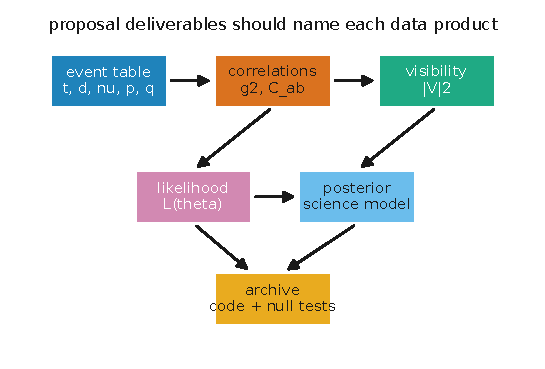
\includegraphics[width=0.88\linewidth]{figures/generated/chapter_22/ch22_data_product_stack.pdf}
\caption{从 proposal 到公开数据的产品链。事件表保留每个光子的到达时间、望远镜、频率、偏振与质量标记；相关器把它变成 \(g^{(2)}\) 与协方差；空间模型给出 \(|V|^2\)；似然与后验把它连到天体参数；归档层要包含代码、版本号与 null test。式 \eqref{eq:e28-data} 里的每个量，都对应这条链上的一环。}
\label{fig:e28-data-products}
\end{figure}

规划数据流程时，有一个贯穿全书的原则值得写进计划的第一页：\textbf{事件表是共同语言}。无论是课堂上的桌面 HBT 演示（第 \ref{chap:e26} 章）、小口径路径验证，还是大设施观测，它们都可以共用同一套"到达时间 + 望远镜 + 频率 + 偏振 + 质量标记"的事件表格式和同一版相关器 \citep{2016SPIE.9907E..0NZ,2025MNRAS.537.2527M}。这意味着你在计划里定义好的数据格式，能让教学、pathfinder 和主设施无缝衔接——这本身就是降低风险、提高可复现性的设计。

\section{风险与里程碑：让计划可以失败，但失败得有价值}
\label{sec:e28-risk}

一份计划如果只写"我们将做什么、预期看到什么"，它其实还没准备好面对现实。现实里目标会比预期暗、系统误差会卡在某个地板、瞬变会触发得太晚。成熟的计划要主动写清\textbf{里程碑}（把成功拆成可验收的节点）和\textbf{风险登记}（把可能翻车的地方连同缓解方案一起列出）。

先说里程碑。一个可执行的里程碑，必须\textbf{同时}指定"测什么"和"算成功的标准是什么"，否则它只是一句愿景。把它写成一个五元组：
\begin{equation}
  m_j=
  \left(
  O_j,\;
  \sigma_{O,j}^{\rm goal},\;
  T_j,\;
  N_{{\rm null},j},\;
  D_{{\rm release},j}
  \right).
  \label{eq:e28-milestone}
\end{equation}
\begin{formulaexplain}
\(m_j\) 是第 \(j\) 个里程碑：\(O_j\) 是要测的可观测量，\(\sigma_{O,j}^{\rm goal}\) 是要达到的目标精度，\(T_j\) 是完成日期或所需观测时间，\(N_{{\rm null},j}\) 是必须通过的 null test 数，\(D_{{\rm release},j}\) 是要发布的数据产品。一个里程碑\textbf{同时钉住}观测量、精度、时间、验证与交付，路线图才不会停在口号上。
\end{formulaexplain}
逐项落地并给出典型取值。\(O_j\) 是可观测量，例如 \(g^{(2)}(0)-1\)、\(|V|^2\)、谱线内外角尺度比、或距离 \(D_A\)。\(\sigma_{O,j}^{\rm goal}\) 是目标精度，直接来自上一节的误差预算 \eqref{eq:e28-error-budget}——里程碑的精度目标不能拍脑袋，必须是误差预算算得出的数。\(T_j\) 是完成日期或所需机时。\(N_{{\rm null},j}\) 是 null test 数：近期项目可要求 \(N_{\rm null}\ge2\)（time-shift 和 off-source 两种）；中期多通道项目应升到 \(N_{\rm null}\ge4\)（再加 off-band、错偏振、注入-恢复）；远期网络项目还要包含链路保真度和存储退相干的独立验收。\(D_{{\rm release},j}\) 是交付的数据产品，例如式 \eqref{eq:e28-data} 里的某个子集加上代码与版本号。把这五项写全，评审就能逐条判断你哪个节点算过关、哪个还欠账。

\begin{figure}[tbp]
\centering
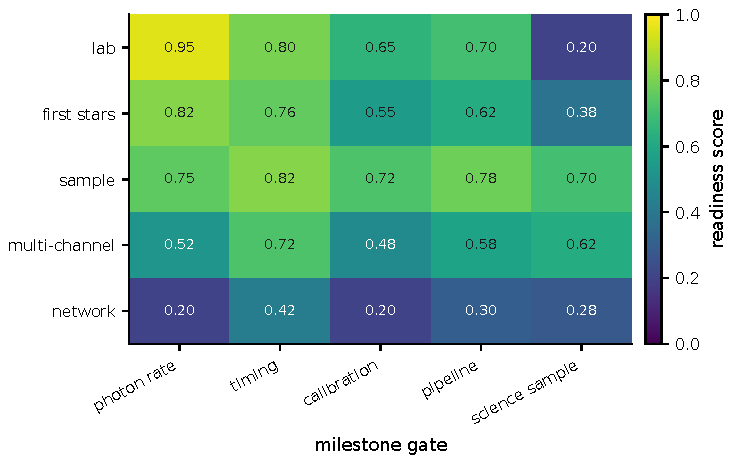
\includegraphics[width=0.90\linewidth]{figures/generated/chapter_22/ch22_milestone_gates.pdf}
\caption{不同阶段的里程碑门槛矩阵。课程实验与第一代恒星强度干涉在光子率、计时和 pipeline 上已较成熟，但多通道校准与网络阶段仍有明显缺口。图中的数字只是 proposal 里应当显式量化的 readiness score \emph{示例}，用来说明式 \eqref{eq:e28-milestone} 各项该怎样打分，并不代表任何设施承诺。}
\label{fig:e28-gates}
\end{figure}

再说风险。风险登记的精髓，是把风险和\textbf{失败判据}（failure criterion）绑在一起写：不仅说"可能出什么问题"，还要说"出到什么程度就该改方案、改到什么"。几个具体例子，都可以用前面的公式量化：若目标星比预期暗 1 mag，由式 \eqref{eq:e28-snr} 光子流下降、信噪比掉到约 \(40\%\)——缓解方案是预先备好更亮的替补目标或延长机时。若系统误差地板停在 \(\sigma_{\rm sys}\sim3\times10^{-5}\)，由式 \eqref{eq:e28-error-budget} 许多 \(|V|^2\) 小信号会被这一项淹没——缓解方案是先建校准星库把 \(\sigma_{\rm cal}\) 压下去。若一次 Type Ia 触发晚了 10 天，外壳更大但光度已下降、模型不确定性 \(\sigma_{\rm model}\) 上升——缓解方案是把触发响应写成硬指标、并对晚到事件设明确的放弃标准。若量子网络链路每天只给出很少的高保真纠缠对，就应把科学模式\textbf{退回}本地模式排序或常规强度干涉，而不是硬撑网络方案（第 \ref{chap:e24} 章）。

\begin{figure}[tbp]
\centering
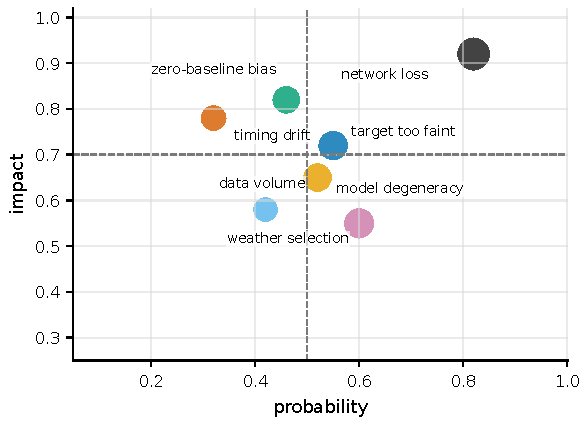
\includegraphics[width=0.86\linewidth]{figures/generated/chapter_22/ch22_risk_register.pdf}
\caption{路线图的风险登记图。横纵轴分别是发生概率与影响，点越大表示现有缓解方案越弱。右上角的风险必须在项目开始前配套缓解：网络损耗要先做短基线 pathfinder，零基线偏差要先建校准星库，目标过暗要预设明确的触发与放弃标准。}
\label{fig:e28-risk}
\end{figure}

这两件事合起来传达一个也许是本章最重要的态度：\textbf{好的研究计划允许自己失败，但要让每一次失败都告诉下一阶段该改什么}。检出为零的一夜，只要留下了定标好的事件表、通过的 null test 和一版公开相关器，就把仪器知识往前推了一步——这远胜于一个"只报告成功"的计划。

\section{把全书串成一条路径：从课程项目到研究课题}
\label{sec:e28-path}

最后，把前面六步拧成一根绳，看看它怎样从一个课堂练习，一路长成一份能提交的研究计划——以及在这条路上，量子网络这类远期设想该被摆在哪里。

起点可以很小。课程项目（第 \ref{chap:e26} 章）从桌面 HBT、事件表模拟、均匀圆盘拟合、SPADE 的 Fisher 信息（第 \ref{chap:e12} 章）和假警报计算开始——这些练习看似玩具，却已经把"提出问题 \(\to\) 设计观测 \(\to\) 估精度 \(\to\) 写计划"这条路径走了一遍缩微版。往上一层，较小的研究题目适合围绕\textbf{一个 pipeline}展开：时间同步、相关器、校准库、目标样本，或一个 open-data notebook——每一个都能独立成篇，也都留得下可复用的产出。再往上，较完整的科学题目可以瞄准 Be 星 \(\mathrm{H}\alpha\) 盘的谱线角尺度、快速自转星的多基线模型、Crab 脉冲星的相位分辨光子统计、Type Ia 距离 toy model 的系统误差，或本地模式排序（第 \ref{chap:e12} 章）与自适应光学的联合实验。最上层，大型合作再把这些课题接到 CTAO/IACT、ELT/VLTI/CHARA、Rubin、SKA、引力波网络，乃至量子网络实验室。

关于\textbf{远期}——量子网络望远镜何时才是主线——计划里要诚实地分层。很多信息学上的好处并不需要完整的量子网络：本地模式排序和相位敏感测量（第 \ref{chap:e12} 章）就能提高小分离、亮度矩估计的信息效率，这是\textbf{现在}就能推进的 \citep{2016PhRvX...6c1033T,2017PhRvL.118g0801T}。two-photon astrometry、单光子辅助或线性光学 pathfinder，目标是把天文光和实验室量子资源稳定地耦合起来，属于中期 \citep{2023PhRvL.130p0801M,2024SPIE13095E..1NR}。真正的纠缠辅助长基线干涉，则需要纠缠分发率、量子存储时间、频率转换效率、Bell 保真度和天文同步\textbf{同时}达标，属于更后面的阶段 \citep{2025PhRvA.111d3701M,2026PhRvA.113a2608P}。这套资源门槛在第 \ref{chap:e24} 章已经写成链路率、存储时间和有效保真度的约束；写计划时只需记住一个数量级：基线 \(B=1000\,\mathrm{km}\) 时光行时 \(B/c\simeq3.3\,\mathrm{ms}\)，地面 km 级基线只要 \(\mu\mathrm{s}\) 到 ms 级同步，但全球或空间基线会把存储与分发压力迅速放大。链路损耗、存储退相干、有用光子率任何一项不达标，网络方案就还不足以取代常规强度干涉——这时诚实的计划应当退回近期能做的那一档，而不是在 proposal 里透支未来。

\begin{figure}[tbp]
\centering
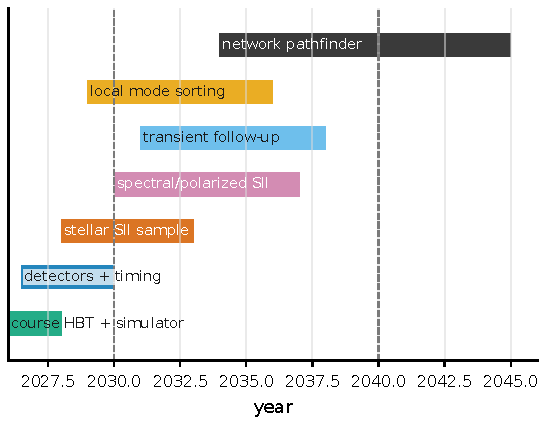
\includegraphics[width=0.92\linewidth]{figures/generated/chapter_22/ch22_program_timeline.pdf}
\caption{从课程 HBT 到量子网络 pathfinder 的阶段性时间线。早期任务建立人才、事件表、计时与校准；中期任务产出第一代科学样本与多通道相关；远期任务只有在本地模式排序、链路与存储指标达标后，才应写成设施级路线。这张时间线正是本章那条"从课程项目长成研究课题"的路径。}
\label{fig:e28-timeline}
\end{figure}

把这一切压成一句可操作的验收标准：\textbf{一份合格的研究计划，至少要列出新增的可观测量、事件表字段、数据估计步骤、每个符号的单位与典型范围、两个以上 null test，以及失败之后仍能留下的数据、代码或仪器约束}。满足这些，你的计划就能被复现、被审查、被改进；否则，"量子"二字就只停留在题目上，没有落到任何一个能被证伪的数字里。这，正是整本书想教给你的最后一件事：把工具变成问题，把问题变成观测，把观测变成一份别人能接着往下做的计划。

\section*{本章要点}
\addcontentsline{toc}{section}{本章要点}

\begin{itemize}
  \item \textbf{顺序不能反。} 先提科学问题、再定可观测量、最后才谈仪器与精度。选目标除了亮度、角尺度、外部先验，还要多问一条："失败后是否仍有产出？"
  \item \textbf{成熟度要可验收。} 用比值向量 \eqref{eq:e28-readiness} 给近期项目打分：光子率、计时、零基线对比度、系统误差、校准样本必须\textbf{同时}达标，任何一项 \(<1\) 都是必须先补的短板。
  \item \textbf{误差预算是地基。} 独立误差按方差相加（式 \eqref{eq:e28-error-budget}），最大项一票否决；统计噪声可用式 \eqref{eq:e28-snr} 估算，信噪比只随 \(\sqrt{\Delta f\,T}\) 增长，精度翻倍要四倍机时，这条要写进可行性小节（第 \ref{chap:e15} 章）。
  \item \textbf{数据流程要工程化。} 把数据产品写成集合 \eqref{eq:e28-data}：延迟直方图、\(|V|^2\)、跨通道协方差与完整协方差矩阵；定义好格式，教学、pathfinder 与主设施才能共用同一套事件表（第 \ref{chap:e13}、\ref{chap:e14} 章）。
  \item \textbf{里程碑与风险同写。} 里程碑五元组 \eqref{eq:e28-milestone} 同时钉住观测量、精度、时间、null test 数与交付；风险要连着失败判据一起写，让计划可以失败，但失败得告诉下一阶段该改什么。
  \item \textbf{远期要诚实分层。} 本地模式排序现在就能做，pathfinder 是中期，纠缠辅助网络要多项指标同时达标才是主线（第 \ref{chap:e24} 章）；不达标就诚实退回近期能做的那一档。
\end{itemize}

\medskip
\noindent\textbf{想一想}
\begin{itemize}
  \item 你手上有一个成熟度向量 \eqref{eq:e28-readiness}，其中光子率一项是 \(R_\gamma/R_{\rm req}=4\)，其余四项都在 \(0.9\) 左右。这个项目该不该现在就写成 proposal？如果不该，你会先把机时和经费投到哪一项上？
  \item 用式 \eqref{eq:e28-snr} 估一估：若把电子带宽 \(\Delta f\) 从 \(200\,\mathrm{MHz}\) 提到 \(800\,\mathrm{MHz}\)，在其余条件不变时，达到同样信噪比所需的积分时间大约缩短到原来的几分之几？
  \item 给你自己选一个第 \ref{chap:e25} 章里的科学案例，试着把它写成一个里程碑五元组 \eqref{eq:e28-milestone}：它的 \(O_j\)、\(\sigma_{O,j}^{\rm goal}\)、\(N_{{\rm null},j}\) 和 \(D_{{\rm release},j}\) 分别该填什么？哪一项你现在还答不上来，说明计划还缺哪一步？
\end{itemize}


% ------------------------------------------------------------
\appendix
\chapter{常用公式索引}
\label{app:a}

公式索引列出每个关系第一次稳定出现的位置。后续章节需要同一组量时，优先回到这里和正文对应处查符号、单位、数量级和适用条件。

\section{事件表、计数和似然}
\label{appsec:a-observables}

\begin{longtable}{p{0.22\linewidth}p{0.31\linewidth}p{0.37\linewidth}}
\toprule
主题 & 位置 & 使用时检查 \\
\midrule
光子事件表字段 & 第 \ref{chap:e00} 章；仪器层扩展见第 \ref{chap:e13} 章 & 时间基准、探测器或望远镜编号、频率通道、偏振、质量标记、空间像素和权重。 \\
时间标定 & 第 \ref{chap:e13} 章 & 原始 TDC 时间、时钟漂移、光路延迟、barycentric 校正和绝对同步。 \\
Poisson 计数 & 第 \ref{chap:e00} 章 & 期望计数是否包含源变化、背景、曝光、选择函数和死时间。 \\
未分箱点过程似然 & 第 \ref{chap:e14} 章 & 事件时间是否保留；rate model 是否随时间、能量或质量窗口变化。 \\
分箱 Poisson 似然 & 第 \ref{chap:e14} 章；教学投影见第 \ref{chap:e26} 章 & bin 宽是否比物理时间尺度、仪器响应和统计计数要求都合适。 \\
延迟和 pair count & 第 \ref{chap:e14} 章 & 延迟窗口、time-shift 背景、随机符合、重复事件和质量筛选。 \\
\(g^{(2)}\) 估计量 & 第 \ref{chap:e14} 章 & 归一化、背景窗口、零延迟峰宽和不相关通道检查。 \\
协方差和后验 & 第 \ref{chap:e14} 章 & 数据点之间是否相关；先验和似然是否写在同一个数据向量上。 \\
\bottomrule
\end{longtable}

\section{相干、可见度和强度干涉}
\label{appsec:a-coherence}

\begin{longtable}{p{0.22\linewidth}p{0.31\linewidth}p{0.37\linewidth}}
\toprule
主题 & 位置 & 使用时检查 \\
\midrule
复可见度 & 第 \ref{chap:e10} 章 & 角坐标单位、投影基线、波长、窄视场近似、带宽平均和源模型。 \\
均匀圆盘 & 第 \ref{chap:e10} 章 & 角直径是半径还是直径；是否需要边缘昏暗；基线是否覆盖第一零点附近。 \\
Siegert 关系 & 第 \ref{chap:e08} 章；空间 HBT 见第 \ref{chap:e10} 章 & 热光、混沌光或高斯场近似是否成立；偏振、频谱和模式数是否改变对比度。 \\
强度干涉观测模型 & 第 \ref{chap:e10} 章；校准模型见第 \ref{chap:e27} 章 & 零基线对比度、峰形、仪器串扰、选择函数和统计噪声是否分开。 \\
相干时间 & 第 \ref{chap:e08} 章；仪器通道形式见第 \ref{chap:e13} 章 & 滤光片带宽、谱线宽度、中心波长和频率单位。 \\
对比度稀释 & 第 \ref{chap:e08} 章 & 电子学响应、相关 bin、有效模式数、偏振平均和光谱平均。 \\
背景稀释 & 第 \ref{chap:e13} 章 & 目标通量分数、夜天光、伴星、谱线连续谱、暗计数和校准星。 \\
强度干涉 SNR & 第 \ref{chap:e10} 章；观测可行性见第 \ref{chap:e15} 章 & 光子率、望远镜面积、积分时间、等效带宽、\(|V|^2\) 和系统误差地板。 \\
基线数 & 第 \ref{chap:e10} 章 & 望远镜数增加会二次增加相关任务；数据率和校准复杂度同步上升。 \\
\bottomrule
\end{longtable}

\section{仪器响应和数据率}
\label{appsec:a-instrument}

\begin{longtable}{p{0.22\linewidth}p{0.31\linewidth}p{0.37\linewidth}}
\toprule
主题 & 位置 & 使用时检查 \\
\midrule
数据率 & 第 \ref{chap:e13} 章 & 采样时间、bit 数、光谱通道数、望远镜数和实时相关器能力。 \\
响应卷积 & 第 \ref{chap:e13} 章 & 探测器脉冲、线缆、放大器、digitizer 和软件相关窗口共同形成的响应核。 \\
jitter budget & 第 \ref{chap:e13} 章 & 探测器 jitter、时钟同步、光纤延迟、触发抖动和 barycentric 校正。 \\
事件表质量筛选 & 第 \ref{chap:e14} 章和第 \ref{chap:e26} 章 & 云层、饱和、死时间附近事件、异常背景、坏通道和目标高度。 \\
校准项分解 & 第 \ref{chap:e27} 章 & 天体项、仪器项、选择函数项和随机误差不能混在一个自由常数里。 \\
\bottomrule
\end{longtable}

\section{估计理论和模式测量}
\label{appsec:a-estimation}

\begin{longtable}{p{0.22\linewidth}p{0.31\linewidth}p{0.37\linewidth}}
\toprule
主题 & 位置 & 使用时检查 \\
\midrule
Fisher 信息 & 第 \ref{chap:e14} 章；空间模式例子见第 \ref{chap:e12} 章 & 参数、数据向量、协方差、导数和先验是否匹配实际观测。 \\
Cramér--Rao 下界 & 第 \ref{chap:e12} 章 & 下界是局部、无偏或渐近条件下的结果；系统误差不自动包含在内。 \\
高斯源量子 Fisher 信息 & 第 \ref{chap:e12} 章 & 源是否为弱、等亮、非相干双点源；PSF 是否已知。 \\
SPADE 模式概率 & 第 \ref{chap:e12} 章 & 模式基、中心定位、串扰矩阵、背景和有限光子数。 \\
SII Fisher 矩阵 & 第 \ref{chap:e12} 章 & \(|V|^2\) 误差、基线覆盖、参数退化和模型假设。 \\
混合统计 & 第 \ref{chap:e27} 章 & 多个独立成分的通量分数按平方稀释相关超额。 \\
Fano factor & 第 \ref{chap:e27} 章 & 慢变源、死时间和 afterpulsing 都能造成非 Poisson 计数。 \\
多重检验 & 第 \ref{chap:e27} 章 & 时间 bin、频率通道、基线、目标数和事后窗口都进入 trial 数。 \\
\bottomrule
\end{longtable}

\section{天体源模型}
\label{appsec:a-sources}

\begin{longtable}{p{0.22\linewidth}p{0.31\linewidth}p{0.37\linewidth}}
\toprule
主题 & 位置 & 使用时检查 \\
\midrule
亮温 & 第 \ref{chap:e16} 章 & 是否处在 Rayleigh--Jeans 近似；角尺度、距离和通量密度是否独立约束。 \\
热辐射和占有数 & 第 \ref{chap:e16} 章 & 频率、温度和模式占有数决定热光统计是否明显。 \\
同步辐射和偏振 & 第 \ref{chap:e16} 章 & 电子能谱、磁场、视角和 Faraday 效应。 \\
Maser 增益 & 第 \ref{chap:e16} 章 & 反转粒子数、速度相干长度、饱和程度和泵浦涨落。 \\
恒星有效温度 & 第 \ref{chap:e17} 章；案例版见第 \ref{chap:e25} 章 & 角直径、bolometric flux、消光和标定星。 \\
双星可见度 & 第 \ref{chap:e17} 章；科学案例见第 \ref{chap:e25} 章 & 通量比、角分离、位置角、多历元轨道和镜像退化。 \\
谱线/连续谱分离 & 第 \ref{chap:e17} 章；案例版见第 \ref{chap:e25} 章 & 谱线通量分数、连续谱角尺度和滤光片泄漏。 \\
瞬变角膨胀 & 第 \ref{chap:e20} 章；案例版见第 \ref{chap:e25} 章 & 触发时间、速度模型、非球对称和历元间演化。 \\
Type Ia 距离 toy model & 第 \ref{chap:e26} 章 & 光球速度、爆炸时间、角半径误差和辐射转移模型。 \\
\bottomrule
\end{longtable}

\section{传播、宇宙学和量子网络}
\label{appsec:a-propagation-network}

\begin{longtable}{p{0.22\linewidth}p{0.31\linewidth}p{0.37\linewidth}}
\toprule
主题 & 位置 & 使用时检查 \\
\midrule
色散延迟 & 第 \ref{chap:e21} 章 & 频率单位、DM 分解、通道内展宽和等离子体近似。 \\
Faraday 旋转 & 第 \ref{chap:e21} 章 & 偏振角约定、频率覆盖、内禀角和前景扣除。 \\
散射卷积 & 第 \ref{chap:e21} 章 & 多径传播、脉冲展宽、去卷积和选择效应。 \\
引力透镜 & 第 \ref{chap:e21} 章 & 质量模型、源位置、时间延迟和 microlensing。 \\
轴子偏振旋转 & 第 \ref{chap:e22} 章 & 频率依赖、时间调制、偏振标定和普通 Faraday 项。 \\
CMB 似然 & 第 \ref{chap:e23} 章 & \(C_\ell\)、协方差、前景和 cosmic variance。 \\
量子网络资源 & 第 \ref{chap:e24} 章 & 链路损耗、存储时间、频率转换、保真度和实际可用的天文光子率。 \\
观测误差预算 & 第 \ref{chap:e15} 章 & 统计、校准、背景、模型和选择函数误差是否都进入。 \\
proposal 里程碑 & 第 \ref{chap:e28} 章 & 可验收观测量、目标精度、null test、交付数据和失败判据。 \\
\bottomrule
\end{longtable}

\chapter{常用单位和数值}
\label{app:b}

这些表格集中列出写作、估算和审稿时最常用的单位与数量级。具体公式回到正文首次定义处；估算时同时检查单位、数量级和适用条件。

\section{基本常数和天文换算}
\label{appsec:b-constants}

\begin{longtable}{p{0.22\linewidth}p{0.30\linewidth}p{0.38\linewidth}}
\toprule
量 & 常用数值 & 使用提醒 \\
\midrule
光速 & \(c=2.998\times10^{10}\,{\rm cm\,s^{-1}}\) & 基线光行时 \(B/c\)：\(1\,{\rm km}\) 约 \(3.3\,\mu{\rm s}\)，\(1000\,{\rm km}\) 约 \(3.3\,{\rm ms}\)。 \\
Planck 常数 & \(h=6.626\times10^{-27}\,{\rm erg\,s}\) & 单个光子能量 \(E=h\nu=hc/\lambda\)。 \\
Boltzmann 常数 & \(k_{\rm B}=1.381\times10^{-16}\,{\rm erg\,K^{-1}}\) & 亮温、Planck 占有数和热噪声都需要它。 \\
Jansky & \(1\,{\rm Jy}=10^{-23}\,{\rm erg\,s^{-1}\,cm^{-2}\,Hz^{-1}}\) & AB 星等和光子率估算常从 Jy 开始。 \\
parsec & \(1\,{\rm pc}=3.086\times10^{18}\,{\rm cm}\) & \(1\,{\rm AU}\) 在 \(1\,{\rm pc}\) 处张角为 \(1''\)。 \\
太阳半径 & \(R_\odot=6.96\times10^{10}\,{\rm cm}\) & 估算恒星角直径和双星尺度时很常用。 \\
太阳光度 & \(L_\odot=3.83\times10^{33}\,{\rm erg\,s^{-1}}\) & 和 \(F_{\rm bol}\)、\(T_{\rm eff}\)、\(\theta\) 联用。 \\
\bottomrule
\end{longtable}

\section{角度、波长和基线}
\label{appsec:b-angle}

\begin{longtable}{p{0.22\linewidth}p{0.30\linewidth}p{0.38\linewidth}}
\toprule
量 & 常用数值 & 相关正文位置 \\
\midrule
角度换算 & \(1\,{\rm rad}=206265''\)；\(1\,{\rm mas}=4.848\times10^{-9}\,{\rm rad}\)；\(1\,\mu{\rm as}=4.848\times10^{-12}\,{\rm rad}\) & 第 \ref{chap:e00} 章、第 \ref{chap:e10} 章。 \\
可见光波长 & 蓝光强度干涉常在 \(400\)--\(450\,{\rm nm}\)；宽波段成像常用 \(500\)--\(800\,{\rm nm}\) & 第 \ref{chap:e10} 章、第 \ref{chap:e15} 章。 \\
衍射量级 & \(\lambda/B\) 在 \(500\,{\rm nm}\)、\(100\,{\rm m}\) 时约 \(1\,{\rm mas}\) & 百米级阵列适合亮星角直径。 \\
第一零点量级 & \(1\,{\rm mas}\) 均匀圆盘在 \(416\,{\rm nm}\) 附近第一零点约 \(100\,{\rm m}\) & 第 \ref{chap:e10} 章。 \\
\(\mu{\rm as}\) 结构 & \(10\,\mu{\rm as}\) 在 \(500\,{\rm nm}\) 下对应 \(\lambda/\theta\sim10\,{\rm km}\) & 近邻超新星、AGN 小尺度结构和远期长基线案例。 \\
投影基线 & \(B_\perp\) 随目标高度、时角和阵列几何变化 & 不能用固定物理基线替代整夜 \(u,v\) 覆盖。 \\
\bottomrule
\end{longtable}

\section{时间、频率和相干}
\label{appsec:b-time}

\begin{longtable}{p{0.22\linewidth}p{0.30\linewidth}p{0.38\linewidth}}
\toprule
量 & 常用数值 & 相关正文位置 \\
\midrule
频率换算 & \(500\,{\rm nm}\) 对应 \(6.0\times10^{14}\,{\rm Hz}\) & 光学带宽常需要在 \(\Delta\lambda\) 和 \(\Delta\nu\) 间换算。 \\
光学相干时间 & \(10\,{\rm nm}\) 级滤光片在可见光下通常给 \(10^{-14}\)--\(10^{-13}\,{\rm s}\) & 第 \ref{chap:e08} 章。 \\
相关 bin & 桌面实验可取 ps--ns；天文强度干涉常受电子学响应和数据率限制 & 第 \ref{chap:e14} 章、第 \ref{chap:e26} 章。 \\
探测器 jitter & 优秀 SPAD、PMT、TDC 系统可到几十 ps--ns；系统同步要单独标定 & 第 \ref{chap:e13} 章。 \\
死时间 & SPAD 常在 ns--\(\mu{\rm s}\)；PMT 和电子链也有恢复时间 & 死时间会在短延迟处制造负相关。 \\
afterpulsing & 概率可到 \(10^{-4}\)--\(10^{-2}\) 量级 & 会在探测器特征延迟处制造正相关。 \\
积分时间标度 & 纯统计误差常按 \(T^{-1/2}\) 下降 & 一旦达到系统误差地板，继续积分不会自动改善。 \\
\bottomrule
\end{longtable}

\section{光子率、星等和背景}
\label{appsec:b-photon-rate}

\begin{longtable}{p{0.22\linewidth}p{0.30\linewidth}p{0.38\linewidth}}
\toprule
量 & 常用数值 & 相关正文位置 \\
\midrule
AB 星等通量 & AB 零点见第 \ref{chap:e15} 章；光子率估算见第 \ref{chap:e00} 章 & 写 proposal 时同时给出带宽、效率、面积和背景。 \\
星等变化 & 目标暗 \(1\,{\rm mag}\)，光子率约降到原来的 \(10^{-0.4}\simeq0.40\) & 第 \ref{chap:e15} 章、第 \ref{chap:e28} 章。 \\
望远镜面积 & \(D=12\,{\rm m}\) 的理想几何面积约 \(113\,{\rm m^2}\)，实际有效面积还要乘效率和遮挡 & Cherenkov 望远镜光学效率、滤光片和探测器 QE 都要进入。 \\
背景稀释 & 目标通量分数为 \(f\) 时，二阶相关超额近似按 \(f^2\) 被压低 & 第 \ref{chap:e13} 章。 \\
窄线观测 & 谱线越窄，相干时间越长，但总光子数和滤光片泄漏可能变差 & Be 星盘、maser/laser 和 BLR 案例都要报告线/连续谱分离。 \\
夜天光 & 随月相、天顶距、滤光片和场镜大小变化 & 不要把暗场背景当成所有目标位置都适用。 \\
\bottomrule
\end{longtable}

\section{仪器和数据量}
\label{appsec:b-instrument}

\begin{longtable}{p{0.22\linewidth}p{0.30\linewidth}p{0.38\linewidth}}
\toprule
量 & 常用数值 & 相关正文位置 \\
\midrule
单路采样数据率 & \(\Delta t=4\,{\rm ns}\)、\(16\) bit、单通道时约 \(4\,{\rm Gb\,s^{-1}}\) & 第 \ref{chap:e13} 章。 \\
多通道膨胀 & 64 个光谱通道会把同一例子推到约 \(256\,{\rm Gb\,s^{-1}}\) 每望远镜 & 需要实时相关、压缩或片上累加。 \\
基线数 & 4 台望远镜为 6 条基线；60 台为 1770 条基线 & 第 \ref{chap:e10} 章。 \\
校准星 & 应尽量接近目标天空位置、颜色和亮度，且角直径已知 & 第 \ref{chap:e15} 章。 \\
质量切片 & 按天空透明度、目标高度、背景率、死时间和通道状态切分 & 只报告墙钟时间不足以复现实验。 \\
系统地板 & \(10^{-5}\)--\(10^{-4}\) 级相关幅度地板已足以支配许多 SII 目标 & 第 \ref{chap:e27} 章。 \\
\bottomrule
\end{longtable}

\section{天体物理数量级}
\label{appsec:b-astro}

\begin{longtable}{p{0.22\linewidth}p{0.30\linewidth}p{0.38\linewidth}}
\toprule
量 & 常用数值 & 相关正文位置 \\
\midrule
亮星角直径 & 近邻亮星常在 \(0.2\)--\(5\,{\rm mas}\) 量级 & 第 \ref{chap:e17} 章、第 \ref{chap:e25} 章。 \\
Type Ia 早期速度 & 光球速度常为 \(8000\)--\(15000\,{\rm km\,s^{-1}}\) & 第 \ref{chap:e20} 章、第 \ref{chap:e26} 章。 \\
近邻超新星角半径 & \(20\,{\rm Mpc}\)、\(v=10^4\,{\rm km\,s^{-1}}\)、15 天时约数 \(\mu{\rm as}\) & km 到十 km 级基线才有明显信息。 \\
Crab 周期 & 约 \(33\,{\rm ms}\) & 相位分辨光子统计需要保留绝对时间。 \\
AGN 宽线区 & 光变延迟常为天到月，角尺度通常极小 & 需要把 reverberation、角位移和模型先验合并。 \\
CMB 温度 & \(2.725\,{\rm K}\) & 第 \ref{chap:e23} 章；光学光子统计不能直接套用。 \\
\bottomrule
\end{longtable}

\chapter{术语表}
\label{app:c}

常用术语按工作定义、容易混用的边界和主要阅读位置列出。定义只保留查阅时最需要的边界；完整物理图像、公式、数量级和文献见正文对应章节。

\section{数据、统计和推断}
\label{appsec:c-data}

\begin{longtable}{p{0.20\linewidth}p{0.45\linewidth}p{0.25\linewidth}}
\toprule
术语 & 本书用法 & 主要位置 \\
\midrule
事件表 & 逐光子记录，至少包含时间和探测通道；可扩展频率、偏振、位置、质量标记和权重。不要把它等同于已经分箱的光变曲线。 & 第 \ref{chap:e00}、\ref{chap:e13}、\ref{chap:e14} 章。 \\
光变曲线 & 事件表在时间轴上的投影，通常丢掉通道、偏振和单事件间隔信息。 & 第 \ref{chap:e00}、\ref{chap:e14} 章。 \\
曝光函数 & 描述有效观测时间、面积、效率和选择函数怎样随时间或通道变化的函数。 & 第 \ref{chap:e14}、\ref{chap:e15} 章。 \\
live time & 扣除死时间、坏天气、饱和和质量筛选后的有效积分时间。 & 第 \ref{chap:e13}、\ref{chap:e15} 章。 \\
Poisson 过程 & 给定瞬时率后，事件独立到达的计数模型；非稳态源要使用随时间变化的率。 & 第 \ref{chap:e00}、\ref{chap:e14}、\ref{chap:e27} 章。 \\
Cox process & 率本身随机变化的 Poisson 过程；可产生 super-Poisson 计数，不必是新物理。 & 第 \ref{chap:e27} 章。 \\
似然 & 在给定模型参数下得到观测数据的概率密度或概率质量。不要和后验混用。 & 第 \ref{chap:e14}、\ref{chap:e15} 章。 \\
后验 & 似然与先验结合后的参数分布。报告后验时要说明先验和数据向量。 & 第 \ref{chap:e14}、\ref{chap:e26} 章。 \\
Fisher 信息 & 似然对参数局部敏感度的度量；不是系统误差的自动替代品。 & 第 \ref{chap:e00}、\ref{chap:e14}、\ref{chap:e12} 章。 \\
协方差矩阵 & 数据点或参数误差之间相关性的矩阵。多基线 \(|V|^2\) 点通常不能默认独立。 & 第 \ref{chap:e14}、\ref{chap:e15} 章。 \\
Fano factor & 计数方差与均值的比值，用于诊断慢变源、死时间和 afterpulsing。 & 第 \ref{chap:e27} 章。 \\
trial factor & 多重检验造成的全局显著性修正。时间 bin、频率通道、基线和目标数都可能贡献 trial。 & 第 \ref{chap:e27} 章。 \\
null test & 应该消除天体信号而保留仪器或背景结构的检查，例如 time-shift、off-source、off-band、错偏振。 & 第 \ref{chap:e14}、\ref{chap:e26}、\ref{chap:e27} 章。 \\
\bottomrule
\end{longtable}

\section{量子光学和相干函数}
\label{appsec:c-optics}

\begin{longtable}{p{0.20\linewidth}p{0.45\linewidth}p{0.25\linewidth}}
\toprule
术语 & 本书用法 & 主要位置 \\
\midrule
模式 & 光场的一个可分辨自由度，可以是空间、时间、频率或偏振模式。模式数决定聚束对比度是否被稀释。 & 第 \ref{chap:e06}、\ref{chap:e08} 章。 \\
占有数 & 单个模式中的平均光子数；射电常大，光学天文单模式常很小。 & 第 \ref{chap:e06}、\ref{chap:e16} 章。 \\
相干态 & Poisson 光子数分布、\(g^{(2)}(0)=1\) 的理想光态；天体 laser/maser 不一定等同于稳定相干态。 & 第 \ref{chap:e06}、\ref{chap:e27} 章。 \\
热态 & 单模式下有聚束的混沌光场；多模式和有限响应会降低观测对比度。 & 第 \ref{chap:e06}、\ref{chap:e08} 章。 \\
压缩态 & 一个正交量噪声低于真空、另一个正交量升高的光场状态；宇宙学涨落中也出现相关语言。 & 第 \ref{chap:e06}、\ref{chap:e23} 章。 \\
密度矩阵 & 描述纯态或混合态的状态对象；当天体光源由许多不可分辨成分组成时特别自然。 & 第 \ref{chap:e06}、\ref{chap:e24} 章。 \\
退相干 & 相位关系因环境、平均或未观测自由度而不可用；不要简单等同于“没有量子”。 & 第 \ref{chap:e06}、\ref{chap:e23} 章。 \\
一阶相干函数 & 描述场振幅相关；振幅干涉和复可见度都依赖这个量。 & 第 \ref{chap:e08}、\ref{chap:e10} 章。 \\
二阶相干函数 & 描述强度或探测事件的相关；HBT 和光子统计的核心观测量。 & 第 \ref{chap:e08}、\ref{chap:e14} 章。 \\
聚束 & 热光或混沌光在零延迟附近的正二阶相关超额。 & 第 \ref{chap:e00}、\ref{chap:e08} 章。 \\
反聚束 & \(g^{(2)}(0)<1\) 的非经典光子统计特征；天文环境中极难保持。 & 第 \ref{chap:e08}、\ref{chap:e27} 章。 \\
相干时间 & 光场一阶相干显著的时间宽度，通常由光谱带宽控制。 & 第 \ref{chap:e00}、\ref{chap:e08} 章。 \\
Siegert 关系 & 热光或高斯场下把二阶相关和一阶相干模平方联系起来的关系。 & 第 \ref{chap:e00}、\ref{chap:e08}、\ref{chap:e10} 章。 \\
Glauber 相关 & 用探测算符定义的量子光学相关函数，是 \(g^{(n)}\) 语言的基础。 & 第 \ref{chap:e06}、\ref{chap:e08} 章。 \\
\bottomrule
\end{longtable}

\section{干涉、成像和模式测量}
\label{appsec:c-interferometry}

\begin{longtable}{p{0.20\linewidth}p{0.45\linewidth}p{0.25\linewidth}}
\toprule
术语 & 本书用法 & 主要位置 \\
\midrule
复可见度 & 天空亮度分布的归一化 Fourier 分量；振幅和相位都属于一阶相干信息。 & 第 \ref{chap:e00}、\ref{chap:e10} 章。 \\
基线 & 两个望远镜之间的矢量间隔；进入可见度的是投影到天空平面的 \(B_\perp\)。 & 第 \ref{chap:e10} 章。 \\
\(u,v\) 覆盖 & 观测在空间频率平面上的采样；决定成像和模型退化。 & 第 \ref{chap:e10}、\ref{chap:e15} 章。 \\
VCZ 定理 & 把非相干远场源的天空亮度与一阶空间相干联系起来的定理。 & 第 \ref{chap:e10} 章、附录 \ref{app:d}。 \\
均匀圆盘 & 恒星角直径的最简单模型；真实恒星常需要边缘昏暗或非球对称修正。 & 第 \ref{chap:e00}、\ref{chap:e10}、\ref{chap:e17} 章。 \\
边缘昏暗 & 恒星盘边缘亮度低于中心的效应，会改变可见度曲线和角直径解释。 & 第 \ref{chap:e17} 章。 \\
强度干涉 & 用强度涨落相关测量 \(|V|^2\)，对大气 piston 相位不敏感，但对背景、时间响应和校准敏感。 & 第 \ref{chap:e10}、\ref{chap:e15} 章。 \\
零基线对比度 & 未被空间分辨率压低时的相关峰幅度，常用于标定仪器稀释因子。 & 第 \ref{chap:e10}、\ref{chap:e15} 章。 \\
相位缺失 & 只测 \(|V|^2\) 时不能直接得到复相位，导致镜像和非对称结构退化。 & 第 \ref{chap:e10}、\ref{chap:e27} 章。 \\
phase retrieval & 从强度或 \(|V|^2\) 约束恢复相位的算法问题，需要先验和多采样。 & 第 \ref{chap:e10}、\ref{chap:e27} 章。 \\
SPADE & 把焦平面场投影到空间模式来估计亚 Rayleigh 分离的测量思想。 & 第 \ref{chap:e12}、\ref{chap:e26} 章。 \\
Rayleigh curse & 直接成像估计小分离双源时 Fisher 信息下降的现象；不是所有测量的极限。 & 第 \ref{chap:e12}、\ref{chap:e27} 章。 \\
量子 Fisher 信息 & 在允许测量集合上参数信息的上限；只有在模型和测量假设满足时才是可达目标。 & 第 \ref{chap:e12} 章。 \\
\bottomrule
\end{longtable}

\section{仪器、探测器和校准}
\label{appsec:c-instrument}

\begin{longtable}{p{0.20\linewidth}p{0.45\linewidth}p{0.25\linewidth}}
\toprule
术语 & 本书用法 & 主要位置 \\
\midrule
SPAD & 单光子雪崩二极管，适合时间标签光子计数；需处理死时间和 afterpulsing。 & 第 \ref{chap:e13} 章。 \\
PMT & 光电倍增管，常用于快速光子计数和 Cherenkov 仪器；增益、脉冲形状和背景要标定。 & 第 \ref{chap:e13}、\ref{chap:e15} 章。 \\
TDC & time-to-digital converter，把探测脉冲转换成数字时间标签。 & 第 \ref{chap:e13}、\ref{chap:e26} 章。 \\
jitter & 探测和计时链造成的时间抖动，会展宽相关峰并稀释对比度。 & 第 \ref{chap:e13} 章。 \\
死时间 & 探测器或电子学在一次事件后短时间不能记录新事件的区间。 & 第 \ref{chap:e13}、\ref{chap:e27} 章。 \\
afterpulsing & 探测器内部陷阱释放造成的延迟伪事件，会产生短延迟正相关。 & 第 \ref{chap:e13}、\ref{chap:e27} 章。 \\
暗计数 & 没有天体光子时的探测事件率；温度和偏压会改变它。 & 第 \ref{chap:e13} 章。 \\
电子串扰 & 一个通道的电子脉冲污染另一个通道，可能伪装成零延迟相关。 & 第 \ref{chap:e13}、\ref{chap:e27} 章。 \\
White Rabbit & 亚 ns 级网络同步技术之一；是否足够取决于相关峰宽和基线模型。 & 第 \ref{chap:e13} 章。 \\
光谱通道 & 事件表中的频率或波长标签；窄通道提高相干时间但降低每通道光子数。 & 第 \ref{chap:e13}、\ref{chap:e28} 章。 \\
偏振通道 & 事件表中的偏振标签；用于区分源物理、散射、Faraday 效应和仪器偏振。 & 第 \ref{chap:e13}、\ref{chap:e22} 章。 \\
校准星 & 用来确定零基线对比度、系统响应或角直径尺度的参考星。 & 第 \ref{chap:e15}、\ref{chap:e28} 章。 \\
系统误差地板 & 积分时间继续增加也不再按 \(T^{-1/2}\) 改善的误差下限。 & 第 \ref{chap:e15}、\ref{chap:e27} 章。 \\
\bottomrule
\end{longtable}

\section{天体源和辐射机制}
\label{appsec:c-sources}

\begin{longtable}{p{0.20\linewidth}p{0.45\linewidth}p{0.25\linewidth}}
\toprule
术语 & 本书用法 & 主要位置 \\
\midrule
亮温 & 把辐射强度表达成等效黑体温度的量；高亮温常提示相干机制或极端小角尺度。 & 第 \ref{chap:e16} 章。 \\
热辐射 & 由温度和光学深度控制的辐射；光学恒星近似热光但并非完美黑体。 & 第 \ref{chap:e16}、\ref{chap:e17} 章。 \\
同步辐射 & 相对论电子在磁场中辐射，常带偏振和非热谱。 & 第 \ref{chap:e16}、\ref{chap:e19} 章。 \\
逆康普顿散射 & 高能电子把低能光子提升到更高能量的过程。 & 第 \ref{chap:e16} 章。 \\
maser & 微波或射电受激辐射源，天体环境中常受速度相干和泵浦涨落控制。 & 第 \ref{chap:e16}、\ref{chap:e27} 章。 \\
自然激光 & 天体中可能的光学/近红外受激辐射候选，不等同于实验室稳定激光腔。 & 第 \ref{chap:e25}、\ref{chap:e27} 章。 \\
宽线区 & AGN 中产生宽发射线的气体区域，可用时间延迟、谱线和角尺度联合约束。 & 第 \ref{chap:e19} 章。 \\
photon ring & 黑洞强引力附近由光子轨道相关路径形成的细结构。 & 第 \ref{chap:e19} 章。 \\
Type Ia 超新星 & 热核超新星，可作为距离指标；强度干涉方案关心光球角半径。 & 第 \ref{chap:e20}、\ref{chap:e26} 章。 \\
千新星 & 双中子星并合后的 r-process 暂现源，多信使延迟和扩散时间是核心量。 & 第 \ref{chap:e20} 章。 \\
GRB 余辉 & 伽马暴后喷流与环境相互作用产生的多波段辐射。 & 第 \ref{chap:e20} 章。 \\
TDE & 恒星被黑洞潮汐撕裂后的暂现事件，可约束黑洞质量和再处理光球。 & 第 \ref{chap:e20} 章。 \\
\bottomrule
\end{longtable}

\section{传播、宇宙学和新物理}
\label{appsec:c-propagation}

\begin{longtable}{p{0.20\linewidth}p{0.45\linewidth}p{0.25\linewidth}}
\toprule
术语 & 本书用法 & 主要位置 \\
\midrule
DM & dispersion measure，电子柱密度造成的频率相关延迟。 & 第 \ref{chap:e21} 章。 \\
RM & rotation measure，磁化等离子体造成的 Faraday 偏振旋转量。 & 第 \ref{chap:e21}、\ref{chap:e22} 章。 \\
散射展宽 & 多径传播把脉冲或相关峰展宽，可能掩盖本征时间结构。 & 第 \ref{chap:e21} 章。 \\
消光 & 尘埃吸收和散射造成的通量降低；会影响光子率和颜色。 & 第 \ref{chap:e21} 章。 \\
透镜方程 & 源位置、像位置和偏折角之间的关系。 & 第 \ref{chap:e21} 章。 \\
时间延迟距离 & 强透镜时间延迟宇宙学中的距离组合。 & 第 \ref{chap:e21} 章。 \\
波动光学透镜 & 当波长、透镜质量和路径差使干涉不可忽略时的透镜现象。 & 第 \ref{chap:e21}、\ref{chap:e22} 章。 \\
轴子双折射 & 轻场耦合导致偏振角随时间或方向变化的效应候选。 & 第 \ref{chap:e22}、\ref{chap:e23} 章。 \\
CMB B 模 & CMB 偏振中的旋度型分量，可来自引力波、透镜或系统误差。 & 第 \ref{chap:e23} 章。 \\
cosmic variance & 只观测一个宇宙导致的大尺度统计不确定性。 & 第 \ref{chap:e23} 章。 \\
standard siren & 用引力波直接给出距离、再结合红移或电磁对应体做宇宙学的源。 & 第 \ref{chap:e20} 章。 \\
\bottomrule
\end{longtable}

\section{量子网络和项目管理}
\label{appsec:c-program}

\begin{longtable}{p{0.20\linewidth}p{0.45\linewidth}p{0.25\linewidth}}
\toprule
术语 & 本书用法 & 主要位置 \\
\midrule
量子网络望远镜 & 用纠缠、量子存储、频率转换或本地模式测量辅助长基线干涉的远期架构。 & 第 \ref{chap:e24}、\ref{chap:e28} 章。 \\
纠缠分发率 & 网络每秒可提供的可用纠缠资源数；链路损耗会迅速压低它。 & 第 \ref{chap:e24} 章。 \\
量子存储 & 暂存量子态或纠缠资源的设备；存储时间需覆盖基线光行时和处理延迟。 & 第 \ref{chap:e24} 章。 \\
Bell fidelity & 实际纠缠态与理想 Bell 态的保真度，用来衡量网络资源质量。 & 第 \ref{chap:e24} 章。 \\
频率转换 & 把天文光或实验室量子资源转换到可传输、可存储或可探测频段。 & 第 \ref{chap:e24} 章。 \\
readiness & 观测量、仪器指标、校准、代码和数据产品是否达到可执行阶段的量化判断。 & 第 \ref{chap:e28} 章。 \\
milestone & 带观测量、目标精度、截止时间、null test 和数据交付的项目节点。 & 第 \ref{chap:e28} 章。 \\
data product & 可复用的数据交付物，例如事件表、相关直方图、\(|V|^2\)、协方差和后验样本。 & 第 \ref{chap:e28} 章。 \\
risk register & 把技术风险、科学风险、概率、影响和缓解方案写在一起的项目表。 & 第 \ref{chap:e28} 章。 \\
失败判据 & 项目开始前定义的放弃或降级条件；例如目标过暗、系统地板过高或触发太晚。 & 第 \ref{chap:e15}、\ref{chap:e28} 章。 \\
\bottomrule
\end{longtable}

\chapter{核心关系的阅读路线和适用边界}
\label{app:d}

正文中反复出现的几个关系在这里并列呈现。每条关系都标出物理假设、第一次使用的位置和后文容易误用的地方；完整公式见附录 \ref{app:a}。

\section{Siegert 关系}
\label{appsec:d-siegert}

Siegert 关系的物理图像在第 \ref{chap:e00} 章建立，量子光学背景在第 \ref{chap:e08} 章展开，空间强度干涉在第 \ref{chap:e10} 章使用。读这几章时按下面几步检查：

\begin{enumerate}[leftmargin=*]
\item 先确认光场是否可以近似为热光、混沌光或高斯随机场。这个条件允许四阶矩分解成二阶矩的组合。
\item 再把一阶相干函数归一化，得到 \(g^{(1)}\) 或空间相干度 \(\gamma_{12}\)。
\item 在理想单模热光中，零延迟二阶相关超额由 \(|g^{(1)}|^2\) 给出。
\item 进入真实仪器后，把有限带宽、有限时间响应、偏振平均、空间模式和背景写成对比度因子。
\end{enumerate}

\begin{longtable}{p{0.24\linewidth}p{0.34\linewidth}p{0.32\linewidth}}
\toprule
检查项 & 满足时可以怎样用 & 不满足时会怎样错 \\
\midrule
热光或高斯场近似 & 可把二阶相关连接到一阶相干模平方。 & 受激辐射、少数发射体或强非平稳源可能改变 \(g^{(2)}\)。 \\
单模或模式数已知 & 聚束峰对比度可被解释为物理相干信息。 & 多模平均会把峰压低，误认为源不相干。 \\
时间响应已知 & 可把理论峰和观测峰联系起来。 & ns 级电子学会把 fs 级光学相干峰稀释到 \(10^{-6}\)--\(10^{-5}\)。 \\
背景已分离 & 相关超额可转成目标的 \(|V|^2\)。 & 夜天光、伴星或连续谱会按通量分数平方稀释信号。 \\
\bottomrule
\end{longtable}

后文写 \(g^{(2)}-1\) 时，同时给出相干时间、相关 bin、有效模式数、背景通量分数和 null test。只有一个零延迟峰高度，还不足以说明它是天体聚束。

\section{van Cittert--Zernike 定理}
\label{appsec:d-vcz}

VCZ 定理把远场非相干源的天空亮度和一阶空间相干联系起来。第 \ref{chap:e00} 章给出复可见度定义，第 \ref{chap:e10} 章把它用于强度干涉，第 \ref{chap:e15} 章把它放进观测设计。使用这条关系时按下面路径走：

\begin{enumerate}[leftmargin=*]
\item 把天体表面亮度写成角坐标上的函数 \(I(\boldsymbol\theta)\)。
\item 把两台望远镜的投影基线除以波长，得到空间频率 \(\boldsymbol u=\boldsymbol B_\perp/\lambda\)。
\item 对亮度做归一化 Fourier 变换，得到复可见度 \(V(\boldsymbol u)\)。
\item 强度干涉只能直接给出 \(|V|^2\)，所以相位、镜像和非对称结构需要额外信息。
\end{enumerate}

\begin{longtable}{p{0.24\linewidth}p{0.34\linewidth}p{0.32\linewidth}}
\toprule
条件 & 在正文中的用法 & 典型破坏来源 \\
\midrule
远场近似 & 恒星、双星、盘和瞬变的角结构可用 \(u,v\) 平面描述。 & 近场实验、空间基线极端几何或未建模波前曲率。 \\
窄带或已处理带宽 & 每个通道可用单一 \(\lambda\) 近似。 & 宽带平均会洗掉高频可见度结构。 \\
源在积分内稳定 & 每个历元有一个可见度模型。 & 爆发、旋转、脉动和快速结构变化会混合不同模型。 \\
亮度非负且模型合理 & phase retrieval 可用先验约束。 & 只靠 \(|V|^2\) 难以区分镜像和复杂非对称结构。 \\
\bottomrule
\end{longtable}

\section{强度干涉的抗大气相位}
\label{appsec:d-atmosphere}

强度干涉对大气 piston 相位不敏感，是因为它测量强度涨落相关，不依赖两路光场的直接相干叠加。这个优点有明确边界：

\begin{itemize}[leftmargin=*]
\item 透明度变化仍在。透明度改变光子率，也改变随机符合和背景归一化。
\item 闪烁仍在。闪烁会在较慢时间尺度上引入强度相关，需要 time-shift 和分块检查。
\item 电子串扰仍在。串扰可产生比天体峰更窄、更高的零延迟结构。
\item 背景稀释仍在。背景即使不相关，也能通过通量分数压低目标信号。
\end{itemize}

使用“抗大气相位”这个优点时，也要报告非相位误差怎样被监测：校准星、off-source、off-band、错偏振、暗场、time-shift 和注入恢复至少选用几项。

\section{Rayleigh 限制和 Fisher 信息}
\label{appsec:d-rayleigh}

Rayleigh 判据是成像经验尺度，并非所有参数估计问题的信息极限。第 \ref{chap:e12} 章展示了直接成像和模式测量的差别，第 \ref{chap:e26} 章把它变成计算实验。使用这组结果时，先检查这些模型要素：

\begin{enumerate}[leftmargin=*]
\item 明确参数：是两点源分离、质心、通量比、角直径，还是更复杂图像。
\item 明确数据：像素强度、模式计数、事件时间，或 \(|V|^2\)。
\item 写出似然或 Fisher 信息；不要只引用“超分辨”这个词。
\item 加入背景、有限光子数、模式错配、像差和质心误差。
\end{enumerate}

SPADE 的结论适用最清楚的情形是弱、等亮、非相干双点源和已知高斯 PSF。换成星系、吸积盘、强透镜弧或含相干成分的源时，需要重新写源模型和测量基。

\section{误差预算和路线图关系}
\label{appsec:d-error-budget}

观测设计中的误差预算见第 \ref{chap:e15} 章，路线图中的 readiness 和 milestone 见第 \ref{chap:e28} 章。误差预算回答目标量能不能测到；路线图回答项目到哪一步才适合投入下一阶段。

\begin{longtable}{p{0.24\linewidth}p{0.34\linewidth}p{0.32\linewidth}}
\toprule
误差项 & 例子 & 应写入的缓解方式 \\
\midrule
统计误差 & 随光子数、积分时间和带宽变化的 shot noise。 & 增加面积、积分时间、通道累加或目标亮度。 \\
校准误差 & 零基线对比度、时间响应、偏振效率和滤光片形状。 & 校准星、实验室响应测量和 nightly calibration。 \\
背景误差 & 夜天光、伴星、连续谱、暗计数。 & off-source、谱线/连续谱分离、背景窗口和通量分数估计。 \\
模型误差 & 边缘昏暗、非球对称、速度模型、辐射转移。 & 多模型比较、后验预测检查和外部观测约束。 \\
选择误差 & 触发、天气、目标样本和事后挑选窗口。 & 预注册目标标准、全局显著性和失败判据。 \\
\bottomrule
\end{longtable}

\chapter{示例计算代码指南}
\label{app:e}

每章对应一个 Python 文件，位置为 \texttt{code/chapter\_XX.py}。这些脚本生成正文 PDF 图，也提供复现实验数量级的起点。公式定义以正文第一次出现处为准；代码把公式变成可检查的曲线、标度、模拟数据和误差预算。

\section{目录和运行顺序}
\label{appsec:e-run}

\begin{enumerate}[leftmargin=*]
\item 先阅读 \texttt{code/README.md}，确认 Python 版本、依赖包和输出目录。
\item 查看 \texttt{code/plot\_style.py} 和 \texttt{code/plot\_recipes.py}，了解统一字体、颜色、线宽和保存函数。
\item 运行单章脚本，例如 \texttt{python code/chapter\_20.py}。单章脚本只应生成该章图，不应改动其他章节。
\item 检查 PDF 是否写入 \texttt{figures/generated/chapter\_XX/}。
\item 编译 \texttt{main\_nature.tex}，确认图号、caption、正文引用和 PDF 版面一致。
\end{enumerate}

\section{脚本和正文的对应关系}
\label{appsec:e-map}

\begin{longtable}{p{0.18\linewidth}p{0.30\linewidth}p{0.42\linewidth}}
\toprule
章节 & 典型图或计算 & 检查重点 \\
\midrule
1--2 & 事件表、Poisson 计数、普通光变曲线和信息丢失 & 图中事件表字段和正文符号一致。 \\
3--4 & 光态、占有数、\(g^{(1)}\)、\(g^{(2)}\)、多模稀释 & 不把理想单模结果画成真实仪器观测值。 \\
5 & 可见度、均匀圆盘、双星、SII SNR、相位缺失 & 坐标轴带单位；基线用 \(B_\perp\)，不要用阵列物理距离替代。 \\
6 & 探测器响应、jitter、死时间、背景稀释、数据率 & 响应核归一化；时间单位清楚。 \\
7 & pair count、time-shift 背景、协方差和 Fisher scaling & 随机符合和物理相关分开画。 \\
8 & Rayleigh curse、SPADE 模式概率、QFI 和 SII Fisher & 小分离极限下不能用 log 轴制造假改善。 \\
9--13 & 辐射机制、恒星、紧致天体、黑洞和瞬变 toy model & 典型参数来自正文；不要只画任意归一化曲线。 \\
14--17 & 传播、偏振、新物理、CMB 和量子网络资源 & 普通天体物理项和新物理项要在图中分开。 \\
18--22 & 误差预算、科学案例、教学实验、误区和路线图 & 图注要说明可行性、失败模式或决策边界。 \\
\bottomrule
\end{longtable}

\section{每张图的最低要求}
\label{appsec:e-figure-requirements}

\begin{longtable}{p{0.24\linewidth}p{0.66\linewidth}}
\toprule
检查项 & 要求 \\
\midrule
物理量 & 坐标轴写清量名和单位；无量纲量要明确写 dimensionless 或省略单位。 \\
数量级 & 至少一个曲线、点或标注应对应正文中的真实数量级。教学放大信号要在 caption 中说明。 \\
符号 & 图中符号应与正文一致，例如 \(B_\perp\)、\(\lambda\)、\(\theta\)、\(R_\gamma\)、\(\Delta t\)、\(\tau_c\)。 \\
输出 & 所有正文图用 PDF，不使用截图或低分辨率位图。 \\
风格 & 使用统一 style；避免过密网格、过多颜色和没有物理含义的装饰。 \\
可复现性 & 脚本顶部或函数注释应说明输入参数、默认值和输出文件。 \\
\bottomrule
\end{longtable}

\section{调试清单}
\label{appsec:e-debug}

若图看起来和正文不一致，优先检查这些问题：

\begin{enumerate}[leftmargin=*]
\item 单位是否混用：mas、rad、m、nm、Hz、s 最容易出错。
\item 角直径是否被当成角半径，或反过来。
\item 基线是否使用投影基线 \(B_\perp\)，而不是阵列物理距离。
\item 光谱带宽是否用 \(\Delta\lambda\) 直接替代 \(\Delta\nu\)。
\item 相关 bin、探测器响应和相干时间是否在同一个时间单位中。
\item 随机数是否固定 seed；模拟图的误差条是否随 seed 大幅改变。
\item 生成的文件名是否和 LaTeX 中的 \texttt{\string\includegraphics} 一致。
\end{enumerate}

\section{课程项目最小提交包}
\label{appsec:e-project-package}

第 \ref{chap:e26} 章的课程项目提交时，至少包含五个文件或对象：事件表说明、Python 脚本、生成的 PDF 图、短报告和 null test 输出。短报告中每张图都要说明输入参数、单位、物理意义和失败模式；只贴图还不够。

\chapter{14 周课程安排建议}
\label{app:f}

这是一套按一学期设计的阅读和项目顺序。课程可以压缩或扩展，但第 \ref{chap:e00}--\ref{chap:e14} 章最好保留；后面的科学案例都依赖事件表、相干函数、仪器误差和相关器语言。

\section{课程目标和评分结构}
\label{appsec:f-goals}

课程结束时，应能从一个科学问题写出观测量、事件表字段、核心公式、数量级、误差预算、null test 和可复现代码。建议评分结构为：每周阅读笔记 \(20\%\)，三次短计算作业 \(30\%\)，一次中期项目设计 \(20\%\)，期末项目报告和代码 \(30\%\)。

\begin{longtable}{p{0.20\linewidth}p{0.34\linewidth}p{0.36\linewidth}}
\toprule
交付物 & 内容 & 评价标准 \\
\midrule
阅读笔记 & 每周 1 页，列出主要观测量、公式、数量级和疑问。 & 是否读懂公式适用条件，不以摘抄摘要代替理解。 \\
短计算作业 & 事件表、\(g^{(2)}\)、可见度、Fisher 信息或误差预算。 & 单位正确、图清楚、代码可运行。 \\
中期设计 & 一个可执行观测或实验方案。 & 光子率、基线、背景、校准和失败判据是否完整。 \\
期末项目 & 代码、PDF 图、短报告和 null test。 & 是否能复现，是否解释系统误差。 \\
\bottomrule
\end{longtable}

\section{第 1--5 周：基础和仪器}
\label{appsec:f-foundation}

\begin{longtable}{@{}p{0.09\linewidth}p{0.21\linewidth}p{0.27\linewidth}p{0.29\linewidth}@{}}
\toprule
周次 & 阅读 & 课堂重点 & 作业 \\
\midrule
1 & 第 \ref{chap:e00} 章 & 事件表、可观测量、单位和数量级。 & 用同一事件表生成光变曲线和一个简单统计量。 \\
2 & 第 \ref{chap:e00}--\ref{chap:e06} 章 & 为什么平均强度不够；常见光态。 & 比较热光和相干光的计数统计。 \\
3 & 第 \ref{chap:e08} 章 & \(g^{(1)}\)、\(g^{(2)}\)、Siegert 关系和多模稀释。 & 画出不同模式数和时间 bin 下的 \(g^{(2)}\) 对比度。 \\
4 & 第 \ref{chap:e10} 章 & VCZ、均匀圆盘、双星和强度干涉 SNR。 & 拟合一个模拟均匀圆盘角直径。 \\
5 & 第 \ref{chap:e13}--\ref{chap:e14} 章 & 探测器、时间同步、相关器和 null test。 & 写一个事件表相关器，并完成 time-shift 检查。 \\
\bottomrule
\end{longtable}

\section{第 6--10 周：源模型和科学问题}
\label{appsec:f-science}

\begin{longtable}{@{}p{0.09\linewidth}p{0.21\linewidth}p{0.27\linewidth}p{0.29\linewidth}@{}}
\toprule
周次 & 阅读 & 课堂重点 & 作业 \\
\midrule
6 & 第 \ref{chap:e12} 章 & Rayleigh curse、SPADE 和 Fisher 信息。 & 比较直接成像和模式测量的小分离误差。 \\
7 & 第 \ref{chap:e16}--\ref{chap:e17} 章 & 辐射机制、热光近似、恒星角直径和双星。 & 用 \(|V|^2\) 区分均匀圆盘和双星 toy model。 \\
8 & 第 \ref{chap:e18}--\ref{chap:e19} 章 & 紧致天体、脉冲星、黑洞和 photon ring。 & 设计一个保留相位或时间标签的事件表。 \\
9 & 第 \ref{chap:e20} 章 & 瞬变触发、角膨胀、多信使延迟。 & 做 Type Ia 或新星角膨胀 toy model。 \\
10 & 第 \ref{chap:e21}--\ref{chap:e23} 章 & 传播、偏振旋转、透镜、新物理和 CMB。 & 区分一个普通传播项和一个新物理候选项。 \\
\bottomrule
\end{longtable}

\section{第 11--14 周：设计、项目和报告}
\label{appsec:f-project}

\begin{longtable}{@{}p{0.09\linewidth}p{0.21\linewidth}p{0.27\linewidth}p{0.29\linewidth}@{}}
\toprule
周次 & 阅读 & 课堂重点 & 作业 \\
\midrule
11 & 第 \ref{chap:e24}--\ref{chap:e15} 章 & 量子网络边界、观测设计和误差预算。 & 写一页观测申请摘要。 \\
12 & 第 \ref{chap:e25} 章 & 第一代科学案例排序。 & 给三个候选项目打 readiness 分数。 \\
13 & 第 \ref{chap:e26}--\ref{chap:e27} 章 & 教学实验、常见误区、假警报和新物理边界。 & 完成项目代码、图和两个 null test。 \\
14 & 第 \ref{chap:e28} 章 & 从教材项目到 proposal。 & 提交期末报告、代码和里程碑表。 \\
\bottomrule
\end{longtable}

\section{期末项目题目库}
\label{appsec:f-project-list}

\begin{longtable}{p{0.25\linewidth}p{0.34\linewidth}p{0.31\linewidth}}
\toprule
题目 & 基本内容 & 推荐扩展 \\
\midrule
桌面 HBT & 事件表、延迟直方图、time-shift、响应核。 & 比较激光、LED 和伪热光。 \\
均匀圆盘拟合 & \(|V|^2\) 模拟、角直径后验、基线覆盖。 & 加入边缘昏暗或校准星误差。 \\
双星强度干涉 & 通量比、角分离、位置角和多基线退化。 & 加入轨道相位和镜像退化。 \\
SPADE toy model & 模式概率、Fisher 信息、串扰和背景。 & 比较不同 PSF 或质心误差。 \\
Type Ia 距离 & 角半径、速度、爆炸时间和距离后验。 & 加入非球对称或速度梯度。 \\
假警报分析 & Poisson 尾部、trial factor、全局显著性。 & 用真实或模拟搜索网格。 \\
\bottomrule
\end{longtable}

\chapter{文献导读}
\label{app:g}

这份导读按阅读目的组织文献。正文各章保留更密集的引用；这里列出进入主题时适合先读的一组。所有条目使用 NASA ADS bib key，并在 \texttt{references.bib} 中维护。

\section{经典起点}
\label{appsec:g-classic}

强度干涉的历史起点是 Hanbury Brown 和 Twiss 的实验与天文实现 \citep{1956Natur.178.1046H,1957RSPSA.242..300B,1974iiia.book.....H}。读这组文献时，重点在于看他们怎样把相关峰、望远镜面积、基线、带宽和积分时间连成一个可执行观测，不要停在 \(g^{(2)}\) 的名字上。量子光学基础可从 Glauber 和 Sudarshan 的相干性理论，以及 Mandel--Wolf 和 Gerry--Knight 的教材进入 \citep{1963PhRv..130.2529G,1963PhRvL..10..277S,1995ocqo.book.....M,1985stop.book.....G}。

\section{强度干涉的现代复兴}
\label{appsec:g-sii}

现代复兴的主线是把 Cherenkov 阵列、大面积望远镜、数字相关器和校准星库合在一起。早期方案和仪器路径可读 \citet{2009A&A...508..531N,2017MNRAS.472.4126G}；真实天文结果从 VERITAS、MAGIC 和后续样本开始进入系统测量阶段 \citep{2020NatAs...4.1164A,2021MNRAS.506.1585Z,2022MNRAS.512.1722K,2024MNRAS.529.4387A,2024ApJ...966...28A,2025ApJ...995..191A}。读这些文章时，优先看数据率、零基线标定、背景扣除、系统误差地板和目标选择，角直径表要放回这些条件里理解。

\section{探测器、计时和事件表}
\label{appsec:g-instrument}

事件表天文学需要把光学、电子学和时间标准读在一起。AQuEye、IquEye 和光子计数仪器论文适合用来理解 ps--ns 级时间标签、绝对同步和高光子率数据流 \citep{2015SPIE.9504E..0CZ,2016SPIE.9907E..0NZ,2013NIMPA.725..187J,2020RScI...91a3108W}。读这组文献时，把探测器效率、死时间、afterpulsing、TDC 分辨率、GPS/White Rabbit 同步和数据格式单独列成表；这些量后来都会进入第 \ref{chap:e13}--\ref{chap:e14} 章的数据模型。

\section{量子估计和亚分辨测量}
\label{appsec:g-estimation}

Rayleigh curse 和 SPADE 的核心文献说明，传统分辨率判据并非所有参数估计问题的信息极限 \citep{2015Optic...2..646T,2016PhRvX...6c1033T,2017PhRvL.118g0801T,2017NJPh...19b3054T}。读这组文献时，把每篇文章的源模型、PSF、背景、可用模式和 Fisher 信息定义列出来；“两点弱非相干源”的结论只在相应条件下使用。

\section{天体辐射机制和源模型}
\label{appsec:g-sources}

恒星、maser、自然激光、Crab 光子统计和紧致天体章节需要同时读经典辐射机制和现代观测。量子光学语言无法替代普通天体物理模型；它的作用是标出哪些光子统计量还没有被平均掉。读这一组文献时，按源类型记录三个量：亮度或光子率、角尺度或时间尺度、以及最可能破坏理想统计的混合成分。对受激辐射和自然激光候选，尤其要区分窄线、高亮温、泵浦涨落和稳定相干态之间的差别 \citep{1982RvMP...54.1225E,1992ARA&A..30...75E,2004A&A...428..497J,2005MNRAS.364..731J,2005NewA...10..361J,2008AIPC..984..216D}。

\section{传播、透镜、偏振和宇宙学}
\label{appsec:g-propagation}

传播章节的文献应按观测量来读：DM 和色散延迟、RM 和偏振角、散射脉冲展宽、尘埃消光、引力透镜时间延迟、波动光学透镜、CMB 偏振和宇宙双折射。每个主题都要问同一个问题：它改变的是到达时间、频率、偏振、相位，还是强度相关？如果这个问题答不清，后文很容易把传播效应误写成源的量子统计。

\section{科学案例和远期网络}
\label{appsec:g-cases}

第一代科学案例可以从亮星角直径、快速自转星、Be 星盘、双星、Crab 光子统计、自然激光和近邻瞬变开始。Type Ia 超新星距离方案展示了强度干涉怎样进入宇宙学距离问题，但同时也暴露了基线、光子率、触发时间和模型系统误差的压力 \citep{2025PhRvD.111h3047K}。量子网络望远镜则应从 pathfinder 读起：two-photon astrometry、纠缠辅助干涉、存储和频率转换的资源约束分别见 \citet{2023PhRvL.130p0801M,2025PhRvA.111d3701M,2025PhRvR...7d3278Z,2026PhRvA.113a2608P,2026Natur.651..326S}。这组文献适合放在课程最后，因为事件表、相干函数、仪器误差和误差预算先熟悉以后，网络方案的资源压力才会清楚。

\section{读文献时的记录模板}
\label{appsec:g-reading-template}

\begin{longtable}{p{0.22\linewidth}p{0.68\linewidth}}
\toprule
记录项 & 写法 \\
\midrule
观测量 & 写出论文实际测的量，例如 \(g^{(2)}(\tau)\)、\(|V|^2\)、角直径、偏振角、延迟或事件率。 \\
数据产品 & 记录论文是否发布事件表、相关直方图、校准表、后验样本或代码。 \\
主要数量级 & 光子率、带宽、时间分辨率、基线、目标星等、背景和积分时间。 \\
核心假设 & 热光、高斯 PSF、均匀圆盘、非相干源、稳定响应、弱信号等。 \\
系统误差 & 背景、死时间、afterpulsing、串扰、校准星、模型误差和选择效应。 \\
可复用图像 & 论文中哪些图可以启发教学图，但不能照搬。 \\
\bottomrule
\end{longtable}


\backmatter
\bibliographystyle{plainnat}
\bibliography{references}
\end{document}
